% Fordítás:
% 1.  pdflatex peldatar.tex
% 2.  makeindex -r -o peldatar.ind peldatar.idx
% 3.  pdflatex peldatar.tex

\documentclass[11pt,a4paper,openany]{book}
\usepackage[T1]{fontenc}
\usepackage[utf8]{inputenc}
\usepackage[magyar]{babel}
%\usepackage{lmodern}
\usepackage{fancyhdr} % A babel elé kell, hogy a fejlécet is magyarĂ­tsa.
\usepackage[magyar]{babel}
\usepackage{graphicx}
\usepackage[top=3cm,bottom=3cm,left=2.5cm,right=2.5cm,bindingoffset=0.5cm]{geometry}
\usepackage{amsmath}%,amsthm}
\usepackage{xurl,xspace}%to break url lines
\usepackage{amssymb}
\usepackage{theorem}
\usepackage{color}
%\usepackage{enumerate}
\usepackage[shortlabels]{enumitem}
\setlist{topsep=0.5em, partopsep=0.5em, parsep=0.5em, itemsep=0em}
\usepackage{ifthen} % A feltételes vezérléshez.
\usepackage{rotating} %Csak Ps->Pdf móddal működik.
\usepackage{tikz}
\usepackage{environ}

%%% Feliratok:
\usepackage[sl]{caption}
\renewcommand{\captionfont}{\sl}
%%%


\usepackage[pdfauthor={Dom},
            pdftitle={Bonyelm Peldatar},
            pdftex,
            hypertexnames=false]{hyperref}
\definecolor{mygreen}{rgb}{0,0.5,0}
\definecolor{myblue}{rgb}{0,0,0.6}
\definecolor{myred}{rgb}{0.6,0,0}
\hypersetup{colorlinks=true,citecolor=mygreen,linkcolor=myblue,urlcolor=myred,
	bookmarks=true,%
	unicode=true
}

\usepackage{index}

\def\magyarOptions{defaults=hu-min,mathbrk=define}
\usepackage[magyar]{babel}

\usepackage{cleveref}

\usepackage[lastexercise,noanswer]{exercise_EGRES}


\newboolean{showComments}
\setboolean{showComments}{true}

\ifthenelse
{\boolean{showComments}}
{
% Ideiglenes komment, a végleges változatban már nem lesz benne:
\newcommand{\wrk}[1]{\textcolor{red}{(\textsl{#1})}}
}
{
% Ilyen, amikor tényleg nincs benne:
\newcommand{\wrk}[1]{}
}

\newcommand{\definition}[1]{\hspace*{-8mm} \textbf{Definíció:} #1 \vspace{2mm}}

% Olyan referencia, ami látszik is az olvasó számára. Egyelőre nem csináltam meg, de tervezem azt a fajta referenciát, ami csak a számomra látszik, hogy konkrétan honnan vettem egy-egy folklór eredményt.
\newcommand{\reff}[1]{(#1)}

% Csak azért használom, hogy kereshető legyen a feladatok közti sztorizás, lehet, hogy végül nem kell majd.
\newcommand{\chat}[1]{#1}

\newcommand{\sol}[1]{
\begin{Answer}
#1
\end{Answer}
}

% \newcommand{\hint}[1]{\textcolor{blue}{\noindent \textbf{Hint:} #1}}

\newcommand{\hint}[1]{\noindent 
\rotatebox[origin=c]{180}{%
\noindent
\begin{minipage}[t]{\linewidth}
\noindent \textbf{Hint:}
#1
\end{minipage}
}%
}

% this didn't cooperate with linking for some reason, not used.
\NewEnviron{Hint}
{%
\noindent
\rotatebox[origin=c]{180}{%
\noindent
\begin{minipage}[t]{\linewidth}
\noindent \textbf{Hint:}

\BODY
\end{minipage}
}%
}%



%%% Fej- és lábléc:
\newcommand{\ttiny}{\small}
\newcommand{\tamopcopy}{}%\sl{\textsf{\ttiny{\copyright\ the authors}}}}
\newcommand{\tkvtarlink}{}%\href{http://www.tankonyvtar.hu}{\sl{\textsf{\ttiny{www.tankonyvtar.hu}}}}}
\pagestyle{fancy}
\fancyhead{} % clear all header fields
\fancyhead[LE,RO]{\sl{\textsf{\ttiny{\thepage}}}}
\fancyhead[LO]{\sl{\textsf{\ttiny{\nouppercase{\leftmark}}}}}
\fancyhead[RE]{\sl{\textsf{\ttiny{Bonyelm p\'eldat\'ar}}}}
\fancyfoot{} % clear all footer fields
\fancyfoot[LE,RO]{\tkvtarlink}
\fancyfoot[LO,RE]{\tamopcopy}
\renewcommand{\headrulewidth}{0.5pt}
\renewcommand{\footrulewidth}{0pt}
\fancypagestyle{plain}{%
\fancyhf{} % clear all header and footer fields
\fancyfoot[LE,RO]{\tkvtarlink}
\fancyfoot[LO,RE]{\tamopcopy}
\renewcommand{\headrulewidth}{0pt}
\renewcommand{\footrulewidth}{0pt}}
%%%

\newcommand{\eps}{\varepsilon}
\newcommand{\biz}[1]{\hspace{1em}{\small#1}}
\newcommand{\fancybiz}[1]{\hspace{1em}{\small#1}}
\newcommand{\cl}[1]{\mbox{\ensuremath{\mathbf{#1}}}\xspace}
% Fontos konkrét bonyolultsági osztályok:
\renewcommand{\P}{\cl{P}}
\newcommand{\NP}{\cl{NP}}
\newcommand{\Ppoly}{\cl{P/poly}}
\newcommand{\PSPACE}{\cl{PSPACE}}
\newcommand{\EXPSPACE}{\cl{EXPSPACE}}
\newcommand{\BPP}{\cl{BPP}}
\newcommand{\RP}{\cl{RP}}
\newcommand{\coRP}{\cl{co\text{-}RP}}
\newcommand{\ZPP}{\cl{ZPP}}
\newcommand{\PP}{\cl{PP}}
\newcommand{\EXP}{\cl{EXP}}
\newcommand{\NEXP}{\cl{NEXP}}
\newcommand{\DTIME}{\cl{DTIME}}
\newcommand{\NTIME}{\cl{NTIME}}
\newcommand{\DSPACE}{\cl{DSPACE}}
\newcommand{\SIZE}{\cl{SIZE}}
\newcommand{\E}{\cl{E}}
\newcommand{\NE}{\cl{NE}}
\newcommand{\LOGSPACE}{\cl{LOGSPACE}}
\renewcommand{\L}{\cl{L}}
\newcommand{\NL}{\cl{NL}}
\newcommand{\coNL}{\cl{co\text{-}NL}}
\newcommand{\coNP}{\cl{co\text{-}NP}}
\newcommand{\PH}{\cl{PH}}
\newcommand{\ACnull}{\cl{AC^0}}
\newcommand{\ACone}{\cl{AC^1}}
\newcommand{\AC}{\cl{AC}}
\newcommand{\NC}{\cl{NC}}
\newcommand{\NCone}{\cl{NC^1}}
\newcommand{\Sigmaone}{\cl{\Sigma_1}}
\newcommand{\Pione}{\cl{\Pi_1}}
\newcommand{\Sigmatwo}{\cl{\Sigma_2}}
\newcommand{\Pitwo}{\cl{\Pi_2}}
\newcommand{\Sigmak}{\cl{\Sigma_k}}
\newcommand{\Pik}{\cl{\Pi_k}}
\newcommand{\Sigmakplus}{\cl{\Sigma_{k+1}}}
\newcommand{\Pikplus}{\cl{\Pi_{k+1}}}
\newcommand{\MA}{\cl{MA}}
\newcommand{\AM}{\cl{AM}}
\newcommand{\TALLY}{\cl{TALLY}}
\newcommand{\SPARSE}{\cl{SPARSE}}
\newcommand{\XP}{\cl{XP}}
\newcommand{\BWBP}{\cl{BWBP}}

% Nyelv:
\newcommand{\la}[1]{\mbox{\sc{#1}}\xspace}
% Konkrét nyelvek:
\newcommand{\SAT}{\la{sat}}
\newcommand{\Language}{\la{L}} % Na ő éppenhogy nem konkrét. És a nevének kellemetlen tulajdonsága, hogy ösztönösen ,,a \\Language''-et Ă­rok.


% A részfeladatokat (a), (b), (c) számozzuk:
\renewcommand{\theenumi}{\alph{enumi}}
\renewcommand{\labelenumi}{(\theenumi)}

\newcommand{\nothing}{\vspace{0mm}}

\newcount\feladatcnt
\def\feladat{\par\advance\feladatcnt1\bigskip\noindent{\bf\the\feladatcnt.}~}
\def\pro{\par\advance\feladatcnt1\bigskip\noindent{\bf\the\feladatcnt.}~}
\def\R{\mathbb{R}}
\def\Z{\mathbb{Z}}
\def\N{\mathbb{N}}
\def\HH{\mathcal{H}}

\newcommand{\hard}{\!\!* }
\newcommand{\veryhard}{\!\!** }
\newcommand{\open}{\!\!**? }
\newcommand{\easy}{\!\!$\heartsuit$ }
\newcommand{\hf}{\!\!$^\textrm{\tiny\textrm{HF}}$ }
\newcommand{\hw}{\!\!$^\textrm{\tiny\textrm{HW}}$ }
\newcommand{\defi}{{\bf Defin\'ici\'o: }}
\newcommand{\pronull}{\hspace{-6mm}{\bf 0. }}
\newcommand{\remark}[1]{\textbf{Megjegyzés:} #1}
\newcommand{\mo}{{\bf Megold\'as: }}


\newcounter{sorszam}

\crefname{sorszam}{}{}

\renewcommand{\ExerciseHeaderTitle}{\ExerciseTitle}

\renewcommand{\ExerciseHeader}{\medskip\noindent
\textbf{\ExerciseHeaderNB .}\ExerciseHeaderDifficulty\ExerciseHeaderTitle
\ExerciseHeaderOrigin}

\renewcommand{\AnswerHeader}{\bigskip\noindent\textbf{\ExerciseHeaderNB .} }

\renewcommand{\QuestionNB}{\alph{Question})\ }

\newindex[thesorszam]{default}{idx}{ind}{TárgymutatĂł}



\begin{document}

\title{Mi a Kolmogorov-bonyolultsága ennek a példatárnak?}

\maketitle

\vspace*{1cm}
\section*{Bevezet\H o}
\addcontentsline{toc}{section}{Bevezet\H o}

\vskip 3em

A példatár az ELTE matematikus és alkalmazott matematikus szak BSc harmadéves Számítástudomány és MSc elsőéves Bonyolultságelmélet tárgyak gyakorlataihoz használt feladatokat és megoldásaik vázlatát tartalmazza.
A forrásfile-ok az EGRES csoport példatárán alapulnak. Köszönet ...
\vskip 3em

\newpage


\vspace{1cm}
\tableofcontents
\newpage


\section*{Jelölések}
\addcontentsline{toc}{section}{Jelölések}

\bigskip
\begin{list}{$\bullet$}{\setlength{\leftmargin}{3ex}}
  \item %\raisebox{1ex}{\includegraphics[height=1ex]{pero.pdf}}
  %konnyu: könnyĹą példa, %dom: mert nincs meg a pero.pdf
      \hard: nehezebb példa, \veryhard: nehéz példa.
      
\item Nyelv: $L$ egy nyelv a $\Sigma$ ábécé felett, ha elemei karaktersorozatok, ahol a karakterek $\Sigma$-beliek. Többnyire $\Sigma=\{a,b\}$ vagy $\Sigma=\{0,1\}$ lesz, ha mást nem mondunk.
\end{list}



\part{Feladatok}

\chapter{Fejt\"or\H ok}

DOMOTOR: Szerintem azokat vegyuk ki, amikben semmi algoritmikus/bonyelmes nincs.

\begin{Exercise}[counter={sorszam}, difficulty=2]
	Adott egy $n \times n$-es tábla. Minden mezőben egy lámpa és egy
	nyomógomb. Ha egy gombot megnyomunk, a sorában és oszlopában lévő összes lámpa
	állapotot vált (égett-elalszik, aludt-kigyullad), a saját lámpáját is beleértve.
	Bekapcsoláskor minden lámpa kikapcsolt állapotban van.
	Ezután valaki odalép a táblához, és össze-vissza
	nyomogatja a gombokat. Feladatunk, hogy helyreállítsuk az eredeti sötét
	állapotot. Hány gombnyomással tudjuk ezt mindig elérni?
	
	\wrk{döm: szerintem ugyanolyan nehéz ez és a következő feladat, legalábbis én egyikre sem látok egyszerűbb megoldást.}
	
	\hint{A feladatot elképzelhetjük úgy, hogy minden gombhoz tartozik egy $GF(2)$ feletti $n\times n$ dimenziós vektor. Szükséges gombnyomások száma $=\log $ Lehetséges állapotok száma $=$ Ahány dimenziós teret feszítenek a vektorok.}
\end{Exercise}

\sol{Ha $n$ páros, akkor az $i.$ sor és $j.$ oszlop összes gombját megnyomva épp csak $(i,j)$ lámpa gyullad ki, tehát a teljes teret feszítik a vektorok.\\	Ha $n$ páratlan, akkor az $i.$ és $j.$ sor (vagy oszlop) összes gombját megnyomva semmi sem történik, tehát ezek a vektorok összefüggőek, azaz egyetlen sor (oszlop) már generálja mindet, tehát legfeljebb $n^2-2(n-1)=(n-1)^2+1$ dimenziós a tér. De ennyinek kell is lennie, hiszen a bal-felső $n-1\times n-1$-es részmátrix gombjaihoz független vektorok tartoznak (hiszen $n-1$ páros) és ezektől független a jobb-alsó sarok vektora.\\
Tehát páros $n$-re $n^2$, páratlan $n$-re $(n-1)^2+1$ gombnyomás kell a kezdeti állapot visszaállításához.}


\begin{Exercise}[counter={sorszam}, difficulty=1]
	Könnyebb a fenti feladatot megoldani úgy, hogy ha a tábla működési
	szabályát kicsit megváltoztatjuk: Gombnyomásra a gomb sorában és oszlopában
	lévő összes lámpa állapotot vált, kivéve magát a gombhoz tartozó lámpát.
	
	\wrk{döm: hint ugyanaz, mint az előzőhöz}
\end{Exercise}

\sol{Itt az $(a,b), (a,d), (c,b), (c,d)$ gombokhoz tartozó vektorok összefüggőek. Tehát az első sor és első oszlop gombjaihoz tartozó vektorok már generálnak mindent, azaz legfeljebb $2n-1$ dimenziós lesz a tér. Az is világos, hogy legalább $2n-2$ dmienziós lesz, mert a bal-felső sarkot beállíthatjuk tetszőlegesre, majd bármely másik két lámpát, melyek egyike az első sorban, a másik az első oszlopban van, tudunk egyszerre kapcsolni egy gombnyomással úgy, hogy a többi lámpa nem változik.\\
	Ha $n$ páratlan, akkor bármely gomb páros sok lámpát kapcsol át az első sor és oszlop uniójából, tehát $2n-2$ dimenziós a tér.\\
	Ha $n$ páros, akkor bármely gomb páros sok lámpát kapcsol át az (első sor és oszlop uniója$\setminus$ bal-felső sarok)-ból, tehát megintcsak $2n-2$ dimenziós a tér.\\
	Tehát $2n-2$ gombnyomás kell a kezdeti állapot visszaállításához.}


\begin{Exercise}[counter={sorszam}, difficulty=0]
	Tekintsük a közismert 15-ös játék azon változatát, amely nem $4 \times 4$-es,
	hanem $2 \times n$-es a táblán játszódik, $n$ darab kék és
	$n-1$ darab piros kővel. Kezdetben a bal felső
	mező az üres, és az alsó sorban vannak a kék kövek.
	Aszimptotikusan hány lépésben tudjuk visszaállítani az
	eredeti állapotot, miután valaki összekeverte a köveket?
\end{Exercise}


\begin{Exercise}[counter={sorszam}, difficulty=0]
	Rajzolás téglalapokkal: Adott egy nulla-egy mátrix. Adjunk hatékony algoritmust, amely minél kisebb számú olyan
	mátrix modulo 2 összegeként állítja elő az adott mátrixot, amely mindenhol nulla,
	csak egy összefüggő (azaz nem kombinatorikus, hanem val\'odi) téglalap-blokkban egy. Elég, ha az algoritmusunk közelíti az
	optimális mátrix-számot.
	
	\hint{ Minden $2 \times 2$-es összefüggő blokkra tekintsük elemei modulo 2 vett összegét.
		Így egy 'duális' mátrixot kapunk, amely értékeit az eredeti négyzetrács keresztezési pontjain veszi fel.
		Könnyen belátható, hogy az eredeti feladat ekvivalens azzal, hogy ezt a mátrixot állítsuk elő
		minél kisebb számú olyan mátrix összegeként, amely egy kétszer kettes, nem okvetlenül összefüggő
		részmátrix elemein egy, azon kívül nulla értékeket tartalmaz. }
\end{Exercise}


\begin{Exercise}[counter={sorszam}, difficulty=0]
	A Gonosz elfog három matematikust. Mindegyiknek a fejére húz egy sapkát. A sapka lehet piros vagy kék, és a Gonosz egyenként, pénzfeldobással dönti el, hogy melyikükön milyen sapka legyen. Nem látják a saját sapkájukat, de látják egymásét. Mikor áttanulmányozták egymás sapkáját, vezényszóra egyszerre meg kell mondaniuk, hogy milyen színű a saját sapkájuk. Három választ adhatnak: piros, kék, passzolok. Ha bármelyikük tévedett (azaz nem passzolt, és nem találta el), akkor végez velük a Gonosz, mert buták voltak. Ha mindegyikük passzolt, akkor is végez velük, mert gyávák voltak.
	
	Mielőtt megkapják a sapkákat, tarthatnak egy taktikai megbeszélést. Adjunk nekik módszert, hogy minél jobb esélyük legyen az életben maradásra. A módszer legyen eredményesebb a nyilvánvaló 50\%-nál, amit például úgy érhetnek el, ha egyikük pirosat mond, a többi passzol.
	
	Mi a legjobb életben maradási esély, ha $n$ matematikus van? (Ez általános $n$-re megoldatlan probléma, oldjuk meg minél többféle $n$ értékre.)
	
	\hint{ A lehetséges sorsolásokat feleltessük meg az $n$-dimenziós kocka csúcsainak. Egy adott játékos helyzete ekkora a kocka valamely élének feleltethető meg. Egy tetszőleges megbeszélt stratégia tehát kódolható ennek az élhálózatnak egy irányításával. A stratégia sikerességének valószínűsége egyenlő \wrk{félbehagyva}. Itt egy kapcsol\'od\'o probl\'ema, amiben mindenki t\"obb sapk\'at kap: \url{https://gilkalai.wordpress.com/2020/12/12/open-problem-session-of-huji-combsem-problem-3-ehud-friedgut-independent-sets-and-lionel-levins-infamous-hat-problem/}}
\end{Exercise}


\begin{Exercise}[counter={sorszam}, difficulty=0]
	Kémként beépültünk egy ellenséges szervezetbe. Ha üzenetet küldünk társainknak, könnyen kiderülhet, és elfoghatnak. Szerencsére az ellenséges szervezet minden nap közzétesz 64 bit információt (ezt elképzelhetjük egy $8 \times 8$-as fekete-fehérrel színezett saktáblának). Mielőtt a kimenő üzenetet publikálnák, átmegy a kezünkön, és nekünk módunkban áll egyetlen, tetszőleges bitet megváltoztatni rajta. Ennek segítségével üzenhetünk haza. Hány bit információt juttathatunk így ki naponta a szervezetből? (A protokollt természetesen még beépülésünk előtt egyeztettük társainkkal.)
\end{Exercise}


\begin{Exercise}[counter={sorszam}, difficulty=0]
	A díszsortűz-feladat: Katonák díszsorfalat állnak. Mindegyik csak a két közvetlen szomszédjával tud kommunikálni, és csak egységnyi időközönként, szinkronizált módon. Az egyes katonák memóriája nagy, de véges konstans. Minden lépésben a memóriájuk állapota, és az előző lépésben hozzájuk bejövő jelzések alapján kimenő jelzéseket adhatnak le szomszédjaiknak. Feladatuk, hogy mindannyian egyidőben adjanak le lövést egylövetű fegyverükből. Ehhez a részletes szabályok a következőek: A nulla időpillanatban megkezdődik a protokoll végrehajtása. Ezután egy előre nem megjósolható időpillanatban a bal szélső kívülről parancsot kap a díszsortűzre. A protokoll akkor helyes, ha véges mennyiségű kommunikációs forduló után mindannyian egyszerre kerülnek a kitüntetett ,,tűz!'' állapotba. Másrészt ezen pillanatot megelőzően egyikük sem kerülhet ,,tűz!'' állapotba, a bal szélsőnek adott parancsot megelőzően sem.
	
	Adjunk számukra protokollt, méghozzá olyat, ahol minél kevesebb lépés telik el a parancs kiadása és a sortűz között. A protokoll nem függhet a sorfal hosszától, és tetszőlegesen hosszú sorfalra is felkészültnek kell lennie. (Tehát olyan sorfalra is, amelynek hossza nem tárolható el a katonák rögzített véges méretű memóriájában.)
	
	\hint{ Először oldjuk meg a feladatnak azt a változatát, ahol a cél az, csak egyetlen katona tüzeljen, méghozzá az, aki pontosan középen áll a sorfalban. (Az egyszerűség kedvéért feltehetjük, hogy páratlan sokan vannak.) }
\end{Exercise}

\sol{ Az egyszerűbb tárgyalás végett a protokollt csak $2^n+1$ hosszú sorfalakra adjuk meg, az általánosítás könnyű, bár munkaigényes.
	
	Először megadunk egy segédprotokollt, amelyet szubrutinként fogunk használni a megoldáshoz. A segédprotokoll célja az, csak egyetlen katona tüzeljen, méghozzá az, aki pontosan középen áll a sorfalban. Itt is feltesszük, hogy a szélen álló által kapott külső parancs indítja a protokollt, feltehetjük, hogy a bal szélről.
	Erre egy egyszer\H u megold\'as, hogy mindenki sorban (kezdve a bal szélről) leteszteli mag\'ar\'ol, hogy \H o-e a k\"oz\'eps\H o \'ugy, hogy mindig ir\'anyba k\"uld egyszerre egy jelet, amik a sor sz\'el\'er\H ol ,,visszapattannak.'' De van egy gyorsabb m\'odszer is.	
	A bal szélen álló indítson el egy ,,piros'' üzenetet jobbra, amelyet a megkapói majd körönként továbbküldenek. Ha a jobb szélsőhöz ér, az ,,pattintsa vissza''. A piros üzenettel egyszerre indítson a bal szélső egy ,,kék'' üzenetet is, amelyet a katonák csak minden harmadik körben küldenek tovább. (Ő maga is csak a harmadik körben indítsa.) Könnyen látható, hogy páratlan hosszú sorfal esetén a piros és a kék üzenet éppen a középső katonánál fog először találkozni. Ő ezt észlelve adja le a lövését, és függessze fel az üzenetek továbbküldését.
	
	Az eredeti feladat megoldásához indítsuk el a segédprotokollt, a következőképpen módosítva: Amikor a középső katona megkapja a két üzenetet, akkor ne tüzeljen, hanem menjen át egy ,,kettévágó'' állapotba, ami alatt azt értjük, hogy ő onnan kezdve a piros üzeneteket nem továbbküldi, hanem visszapattintja, mintha a sor szélén állna. Ezzel egyidőben indítsa el a segédprotokollt mindkét irányba egyszerre. (Két, őt is beleértve $2^{n-1}+1$ méretű rész-sorfal felé.) Kellő idő elteltével a sorfal negyedénél és háromnegyedénél állók (egyszerre) kerülnek kettévágó állapotba, és elindítják a saját két-két részprotokolljukat. Ez a rekurzív folyamat akkor ér véget, amikor az utolsó körben minden páros sorszámú katona kettévágóvá válik. (A páratlan sorszámúak már korábban azzá váltak.) A megoldás befejezéséhez csak azt a kiegészítést kell tennünk, hogy a kettévágó katonák minden körben értesítik szomszédaik kettévágó mivoltukról. Ha egy katona érzékeli, hogy ő és összes szomszédja kettévágó, akkor leadja a lövést, és felfüggeszti működését.

	Ha $N$ katona van a sorfalban, akkor a fenti algoritmus $3N$ ($\pm$ konstans) l\'ep\'es, de az optimum $2N-2$ l\'ep\'es. Ehhez 1, 3, 7, 15 stb.\ lass\'us\'ag\'u jeleket k\"uld a  bal széls\H o. Ezeknek a jeleknek a k\"uld\'es\'et is meg lehet oldalni 6 \'allapottal (nem ismert, hogy 5 el\'eg-e).
	L\'asd: \url{https://en.wikipedia.org/wiki/Firing_squad_synchronization_problem}.
	P\'ar ehhez kapcsol\'od\'o \'ujabb cikk:
	\url{https://arxiv.org/abs/1909.05406}, \url{https://arxiv.org/abs/1909.05408}. }







\chapter{V\'eges Automat\'ak}

\section{DFA}

\defi Véges automata: $M=(Q,\Sigma,\delta,q_0,F)$ véges automatának $Q$ az állapotainak halmaza (véges sok), $\Sigma$ ábécé felett van értelmezve, $\delta$ az átmeneti függvénye (azaz adott betűt olvasva egy állapotban milyen új állapotba kerülünk), $q_0$ a kezdőállapota, $F$ a végállapotainak halmaza. Azon szavak halmazát, melyeket elolvasva az automata valamelyik végállapotába kerül, $L(M)$-lel jelöljük. Azt is mondjuk, hogy $M$ felismeri az $L(M)$ nyelvet \'es elfogadja az $L(M)$-beli szavakat.
R\'eszletesebben l\'asd: \url{http://en.wikipedia.org/wiki/Deterministic_finite-state_machine}. 

\begin{Exercise}[counter={sorszam}, difficulty=0]
	Legyen $Q=\{q_0,q_1\}$, $F=\{q_1\}$ és $\delta(q_i,a)=q_i$ és $\delta(q_i,b)=q_{1-i}$. Milyen nyelvet ismer fel ez az automata?
\end{Exercise}
\begin{Answer}
	Amikben p\'aratlan sok $a$ bet\H u van.
\end{Answer}

\begin{Exercise}[counter={sorszam}, difficulty=0]
	Adjunk véges automatát, mely az alábbi nyelveket ismeri fel!\\
	a) $L=$ a $baba$-t tartalmazó szavak.\\
	b) $L=$ az $abba$-t nem tartalmazó szavak.\\
	c) $L=$ azon szavak, melyek utolsó előtti betűje $b$.\\
	d) $L=$ azon szavak, melyekben bármely egymásutáni öt karakterből legalább kettő $a$.\\
	e) $L=$ magyar (.hu v\'eg\H u) email c\'imek.
\end{Exercise}


\begin{Exercise}[counter={sorszam}, difficulty=0]
	Tal\'alj ki egy nyelvet, amir\H ol tudod, hogy regul\'aris-e, de a padt\'arsad nem!
\end{Exercise}


\begin{Exercise}[counter={sorszam}, difficulty=0]
	Mutasd meg, hogy van olyan nyelv, amit semely véges automata sem tud felismerni! (Ezeket {\em nem reguláris} nyelveknek hívjuk.)
\end{Exercise}	 
\begin{Answer}
	I. Nyelvb\H ol kontinuum sok van, automat\'ab\'ol viszont csak megsz\'aml\'alhat\'o sok.\\
	II. Az $a^{n^2}$ egy konkr\'et nyelv, amir\H ol k\"onnyen bel\'athat\'o, hogy nincs hozz\'a automata, hiszen $a$-kat olvasva ciklusba esne, \'igy van egy olyan $c$, hogy ha $a^{n^2}$-et elfogadja, akkor $a^{n^2+c}$-t is.
\end{Answer}


\begin{Exercise}[counter={sorszam}, difficulty=0]
	Adott két automata, melyek az $L_1$ ill. $L_2$ nyelveket ismerik fel. Adj automatát, amely felismeri az\\
	a) $\bar L_1$ (azaz $L_1$ komplementer) nyelvet,\\
	b) $L_1 \cup L_2$ nyelvet,\\
	c) $L_1 \cap L_2$ nyelvet,\\
	d)\hard $L_1L_2$ nyelvet. (Azaz olyan szavak, melyek felbonthatók egy $L_1$ és egy $L_2$-belire.)
\end{Exercise}
\begin{Answer}
	a) Cser\'elj\"uk meg az elfogad\'o \'es az elutas\'it\'o \'allapotokat.\\
	b-c) Vegy\"uk a k\'et automata \'allapotter\'enek szorzat\'at ($Q_1\times Q_2$) \'es azon defini\'aljuk, hogy hogyan kell tov\'abbl\'epni.\\
	d)~\hard Itt $Q_1\times P(Q_2)$ lesz az \'uj \'allapott\'er, ahol $P$ a hatv\'anyhalmazt jel\"oli.
\end{Answer}


\begin{Exercise}[counter={sorszam}, difficulty=1]\label{2DFA}
	A kétirányú véges automata abban különbözik a hagyományostól, hogy nem kötelező mindig a következ\H o bet\H ut kérnie, hanem visszamehet az előzőhöz is. (Ez bele van kódolva $\delta$-ba, hogy mikor merre lép.) Mutasd meg, hogy bármely ilyen automatához létezik egy egyirányú, amely pont ugyanazt a nyelvet ismeri fel!
	\hint{ Minden jobbra l\'ep\'esn\'el jegyezz\"uk fel, hogy ha az eredeti automata balra \'atl\'epne, akkor milyen \'allapotban t\'erne vissza.	Egy ilyenb\H ol mindig ki tudjuk sz\'amolni a k\"ovetkez\H o ilyet; ut\'ana a r\'egit t\"or\"olhetj\"uk, hogy a mem\'oria konstans maradjon. }
\end{Exercise}	
\begin{Answer}
	\wrk{Az alábbiakban csak ész nélkül beegereztem Németh András rendkívül zavarosan leírt megoldását. Megfésülendő, köszönetnyilvánítandó.}
	\wrk{döm: Átírkáltam kicsit, még zavaros.}
	Azt kell megmutatnunk, hogy ha $A$ egy kétirányban mozgó véges automata, akkor egyirányúvá alakítható. Feltehetjük, hogy $A$ csak akkor kerülhet végállapotba, amikor a ,,bemenet vége'' szimbólumot ovassa.
	Az új automata konstrukciójának kulcsa egy $f: S \rightarrow S\cup \{\bot\}$ függvény kiszámítása (azaz az új automata ezt mindig számolja ki és jegyezze meg, ez megtehető, mivel ez konstans tárat igényel), ahol $S$ az $A$ automata
	állapottere, $\bot$ pedig egy $S$-ben nem szereplő szimbólum. Az $f$ az
	jelenti, hogy az adott pillanatban ha $A$ balra lép és $s$ állapotba
	kerül, akkor amikor legközelebb visszajut a lépés előtti pozícióba a fej,
	akkor milyen állapotban lesz, ill. $f(s)=\bot$, ha valami baleset történik $A$-val mielőtt visszatérne (végtelen ciklus, elakadás, lefutás balra a
	szalagról, ...). Világos, hogy $f$ értékét teljesen
	meghatározzák az automata mozgási szabályai és az aktuális pozíciót megelőző
	input szakasz. Sőt, az is látható, hogy valójában $f$ meghatározásához elég
	az $f$ előző pozícióbeli értéke. Tehát az új automata úgy fog működni, hogy
	egy adott helyzetben az $f$ segítségével ,,szimuláljuk'' $A$
	működését, ill. annak azokat a pillanatait, amikor a fej éppen az aktuális
	pozícióban van, egészen addig, amíg egy jobbra lépés nem következik, amikor
	is jobbra lépünk mi is, áttérünk a megadott új állapotba, és meghatározzuk az új
	$f$-et. Miután végigolvastuk a szót, így megtudjuk, hogy az $A$ automata milyen állapotban állt le.
%Az összes szimuláció és az új $f$ meghatározása játék már az automata konstrukciójakor lejátszható, így azok nem mások, mint egy mapping az új automata állapotterében.
\end{Answer}

\begin{Exercise}[counter={sorszam}, difficulty=2]
	Azt mondjuk, hogy $x$ r\'eszsorozata $y$-nak, ha $x$-et megkaphatjuk $y$-b\'ol n\'eh\'any karakter kit\"orl\'es\'evel. Adott $L$ nyelv eset\'en jel\"olje $SUBSEQ(L)$ azon szavak halmaz\'at, amik valamely $L$-beli sz\'o r\'eszsorozatai. Mutasd meg, hogy tetsz\H oleges $L$ eset\'en $SUBSEQ(L)$ felismerhet\H o v\'eges automat\'aval, ha\\
	a) a $\Sigma$ ábécé k\'etelem\H u,\\
	b) b\'armely v\'eges $\Sigma$ ábécé eset\'en.
\end{Exercise}
\begin{Answer}
	Ez a Higman lemma: \url{https://en.wikipedia.org/wiki/Higman%27s_lemma}.
		A l\'enyeg, hogy a Dickson lemma er\H osebb verzi\'oja igaz: ha valami v\'egesen gener\'alt, akkor bel\H ole v\'eges sok is v\'egesen gener\'alt. Ezt lehet bizonz\'itani indukci\'oval \'es v\'egtelenes Ramsey-vel. Ezutan indukci\'oval bizony\'itjuk az \'all\'it\'ast. Kett\H ore vesz\"unk valamit, ami nincs benne, ezt kieg\'esz\'itj\"uk altern\'al\'ova, enn\'el t\"obb altern\'al\'as nem lehet, $\Z$-re Dickson. H\'aromra 123123..-ra eg\'esz\'itj\"uk ki. Egy sz\'ora vessz\"uk, am\'ig csak 1,2 v\'altakozik, azt\'an 2,3 v\'altakoz\'ast, 3,1-et stb., ilyenekb\H ol nem lehet t\"obb, mint 123-as sz\'o hossza, megint lehet Dicksonozni.
		
		Egy m\'asik neh\'ez feladat: \url{http://en.wikipedia.org/wiki/Star_height_problem}.	
	\end{Answer}
	%
	
	
	\begin{Exercise}[counter={sorszam}, difficulty=0]
		Bemenet tizes sz\'amrendszerbeli sz\'am. Jegyeit v\'altakoz\'o el\H ojellel adjuk \"ossze, majd ezt ism\'etelgess\"uk, am\'ig egyjegy\H u sz\'amot nem kapunk. Mutassuk meg, hogy azon sz\'amok nyelve, amikre null\'at kapunk, regul\'aris.\\
		b)~\veryhard Mi a helyzet, ha csak minden m\'asodikat \"osszeadunk (a t\"obbit meg elfelejtj\"uk) \'es ezt ism\'etelgetj\"uk?
	\end{Exercise}
	\begin{Answer}
		a) Ez pont a 11-es marad\'ek lesz, amit k\"onny\H u kisz\'amolni.
		Forr\'as: Sz\"ogi Evelin feladata.\\
		b) Bocsi, de \'en sem tudom...
	\end{Answer}
	
	\begin{Exercise}[counter={sorszam}, difficulty=0]
		Pumpálós lemma: $\forall L \textit{ reguláris } \exists n \textit{ } \forall z\in L, |z|\geq n \textit{ }\exists u,v\ne \emptyset,w:\textit{ } z=uvw \textit{ és } |uv|\leq n \textit{ és } \forall i\textit{ } uv^iw\in L$.
	\end{Exercise}
	\begin{Answer}
		Ez a pump\'al\'os lemma: \url{https://en.wikipedia.org/wiki/Pumping_lemma_for_regular_languages}.
		L\'enyeg, hogy v\'eges sok \'allapot miatt el\H obb-ut\'obb ugyanabba l\'ep \'ujra a g\'ep.
	\end{Answer}
	
	\begin{Exercise}[counter={sorszam}, difficulty=0]
		Döntsük el, hogy az alábbi nyelvek regulárisak-e!\\
		a) prímszámok egyes számrendszerben.\\
		b) négyzetszámok egyes számrendszerben.\\ 
		c) négyzetszámok kettes számrendszerben.\\
		d)~\hard prímszámok kettes számrendszerben.
	\end{Exercise}
	\begin{Answer}
		a-b) Trivi pump\'al\'os lemm\'ab\'ol. Un\'aris regul\'aris nyelvek karakteriz\'aci\'oja is egyszer\H u.\\
		c) $2^{2n}$ \'es $(2^n+1)^2$ k\"oz\'e bepump\'alhatunk.\\
		d) I. Pump\'al\'as $x$-et $ax+b$-be viszi (ahol $a=2^k$).
		Vegy\"uk ennek a transzform\'aci\'onak az orbitjait mod $p$.
		Ha kezdetben $p$ osztja $x$-et, akkor $p!$ l\'epes ut\'an is osztani fogja (ha $p\ne 2$).\\
		II. Az \'atmeneti m\'atrix miatt valamely polinomokra az $n$ hossz\'u szavak sz\'ama $p_1(n)\lambda_1^n+\ldots+p_k(n)\lambda_k^n$, ez nem lehet $2^n/n$.\\
		III. (Borda Bence) Bauer Mih\'aly t\'etel (Dirichlet speci\'alis esete) szerint v\'egtelen sok $p=k2^n+1$ alak\'u pr\'im van. Pump\'al\'as ut\'an $k2^{n+id}+1$, ami $i=p-1$-re oszthat\'o $p$-vel kis-Fermat miatt.
		
		Egy hasonl\'o feladat: \url{http://cstheory.stackexchange.com/questions/2083/proving-the-set-of-powers-of-2-over-ternary-alphabet-to-be-non-regular/2086#2086}.
	\end{Answer}
	
	
	\begin{Exercise}[counter={sorszam}, difficulty=0]
		a) Van-e olyan $S\subset \N$, ami kettes számrendszerben reguláris, de egyesben nem?\\
		b) És fordítva?\\
		c)~\veryhard És olyan, ami kettesben és hármasban is reguláris, de egyesben nem?
	\end{Exercise}	
	\begin{Answer}
		a) Van, pl.\ $2^n$.\\
		b) Nincs.\\
		c) Nem tudok egyszer\H u bizony\'it\'ast, kij\"on a Cobham T\'etelb\H ol: Let $S$ be a set of non-negative integers and let $m$ and $n$ be multiplicatively independent positive integers. Then $S$ is recognizable by finite automata in both $m$-ary and $n$-ary notation if and only if it is ultimately periodic.
		\url{https://arxiv.org/abs/1801.06704}.
		%ezt nem ertem, csak ezt: http://www.emis.ams.org/journals/BBMS/Bulletin/bul942/BRU.PDF
	\end{Answer}
	
	
	\section{NFA}
	
	\defi Nemdeterminisztikus véges automata: Ugyanaz, mint a determinisztikus, csak egy állapotból többfelé is léphet. (A gráfjában egy csúcsból több azonos indexű él is kiléphet.) Akkor fogad el egy szót, ha van legalább egy olyan futása, ami elfogadja.
	
	\begin{Exercise}[counter={sorszam}, difficulty=0]
		Mutasd meg, hogy a nemdeterminisztikus v\'eges automaták is csak reguláris nyelveket ismernek fel, azaz minden nemdeterminisztikus véges automatához van egy determinisztikus, ami ugyanazt a nyelvet fogadja el!
	\end{Exercise}	
	\begin{Answer}
		\'Ugy csin\'alunk nemdeterminisztikus $N$ automat\'ab\'ol egy determinisztikus $M$ automat\'at, hogy az $M$ minden \'allapota az $N$ lehets\'eges \'allapotainak egy r\'eszhalmaza. Az $a$ c\'imk\'ej\H u \'el a $(q_1,..,q_k)$-b\'ol
		a $\{q\mid \exists i q_i \stackrel a\to q\}$-ba megy.
		Azok a $(q_1,..,q_k)$ \'allapotok elfogad\'ok, amikben van $N$-beli elfogad\'o \'allapot, a $START$ pedig a $(q_{START})$ \'allapot.
	\end{Answer}
	
	\begin{Exercise}[counter={sorszam}, difficulty=0]
		Adott $L$ nyelvre $L^*$ azon szavak nyelve, amik előállnak néhány $L$-beli szó konkatenációjaként. Mutasd meg, hogy ha $L$ reguláris, akkor $L^*$ is!
	\end{Exercise}	
	\begin{Answer}
		Nemdeterminisztikus automat\'aval k\"onny\H u, mert meg tudjuk tippelni, hogy hol \'ernek v\'eget az $L$-beli szavak.
		Ha adott $L$-et elfogad\'o determinisztikus $M$ automata, akkor csin\'alunk bel\H ole egy $L^*$-ot felismer\H o nemdeterminisztikus $N$ automat\'at. Az $N$ \'allapotai ugyanazok lesznek, csak lesz benne p\'ar plusz \'el: az \"osszes $M$-beli elfogad\'o\'allapotb\'ol vezessen \'el pontosan ugyanazokba a cs\'ucsokba is, mint a $START$ \'allapotb\'ol.
	\end{Answer}

	\begin{Exercise}[counter={sorszam}, difficulty=0]
		Annak eldöntése, hogy egy nemdeterminisztikus véges automata az üres nyelvet
		ismeri-e fel, \NL-teljes.
	\end{Exercise}
	
	
	\begin{Exercise}[counter={sorszam}, difficulty=1]
		Ismeretes, hogy egy DFA-hoz polinomidőben meg tudjuk keresni a legkisebb
		állapotszámú ekvivalens DFA-t. Bizonyítsuk be, hogy az analóg NFA-minimalizálási feladat
		akkor és csak akkor oldható meg polinomidőben, ha $\P = \NP$.
		
		\hint{ Építsünk a CNF-hez olyan NFA-t, amely éppen a nemkielégítő értékeléseket fogadja el. }
	\end{Exercise}

	
	
	\begin{Exercise}[counter={sorszam}, difficulty=1]
	Az altern\'al\'o v\'eges automata egy nemdeterminisztikus v\'eges automata, melynek minden állapotához hozzá van rendelve {\bf A} vagy {\bf B}. Ez két játékos, akik előre látják az inputot, az {\bf A} jelű állapotoknál {\bf A}, a {\bf B} jelű állapotoknál {\bf B} dönt, hogy melyik állapotba lépjen tovább az automata. {\bf A} célja, hogy az automata elfogadó állapotba érjen a szó végén, míg {\bf B} célja, hogy ne. Akkor fogad el egy szót az automata, ha {\bf A}-nak van rá nyerő stratégiája, az elfogadott szavak nyelvét pedig ``felismeri'' az automata. Mutasd meg, hogy az altern\'al\'o v\'eges automaták is csak reguláris nyelveket ismernek fel!
\end{Exercise}	 
\begin{Answer}
	Lehets\'eges \'allapotok halmaz\'an csin\'aljunk egy nemdeterminisztikus automat\'at. Ha {\bf B} j\"on, akkor \"osszes lehets\'eges m\'odon l\'ep\"unk, ha {\bf A} j\"on, akkor pedig helyesen tippelve a ``j\'o ir\'anyba'' (ha van ilyen).
\end{Answer}
	
	
\begin{Exercise}[counter={sorszam}, difficulty=0] 	Randomizált véges automata: Ugyanaz, mint a nemdeterminisztikus, csak minden éléhez hozz\'a van rendelve egy valószínűség, ez határozza meg, hogy merre mekkora eséllyel lép. Akkor fogad el egy szót, ha a futásainak $\ge\frac{2}{3}$-a elfogadja és akkor utasítja el, ha a futásainak $\le\frac{1}{3}$-a fogadja el. Akkor ismer fel egy nyelvet, ha a nyelvbeli szavakat mind elfogadja és a nem nyelvbeli szavakat mind elutasítja (tehát semelyik szóra sem lehet határozatlan).\\
	a)~\hard Mutasd meg, hogy van olyan kétirányú (l\'asd \ref{2DFA}. feladat) randomizált véges automata, ami felismeri az $L=\{a^nb^n\}$ nyelvet!\\
	b)~\veryhard Mutasd meg, hogy egyirányú randomizált véges automata csak reguláris nyelveket tud felismerni!\\
	c)~\veryhard Ha csak $poly(n)$ v\'eletlen bitet haszn\'alhat, akkor csak reguláris nyelvet ismerhet fel.\\
	d) Ha a $poly(n)$ v\'eletlen bitet egy k\'etir\'anyban olvashat\'o szalagon kapja az automata, akkor felismerhető a $\{0^n1^n\}$ nyelv.	
	\hint{ b) Próbáljunk felváltva a bal és jobb oldalról beérni középre.\\
	d) Egy $n^{100}$ hosszú sorozatban szinte mindig van pontosan $k$ egymás utáni $1$-es minden $1\le k\le 2\log n$-re. Ha $1\le a<b\le n$, akkor van $k\le \log n$, hogy $a\ne b$ mod $k$.}
\end{Exercise}
\begin{Answer}
	a) K\"oz\'epr\H ol bolyongjunk \'es sz\'amoljuk, hogy mikor melyik v\'eg\'ere \'er\"unk.\\
	b) Legyen $x\sim y$, ha minden $z$-re $xz\in L \Leftrightarrow yz\in L$. Ha v\'egtelen sok ilyen oszt\'aly lenne, akkor lenne egy $x,y$ p\'ar, ami k\"ozel van abban az \'ertelemben, hogy minden \'allapotban kb.\ ugyanakkora es\'ellyel van a randomiz\'alt automata miut\'an elolvasta \H oket. De ekkor minden $z$-re is kb.\ ugyanakkor\'ak lesznek az es\'elyek.
\end{Answer}

\section{Form\'alis nyelvek}


\begin{Exercise}[counter={sorszam}, difficulty=1]
	Adjunk példát \NL-teljes környezetfüggetlen nyelvre. \wrk{Sipser 8.17 van. Nem tudom a megoldást.}
\end{Exercise}


\begin{Exercise}[counter={sorszam}, difficulty=0]
	A \la{CFG-EMPTY} döntési feladat egy instanciája \wrk{Kati nem szereti a szót, inkább körbeírná. Vagy esetleg lehet ,,bemenet''.} egy környezetfüggetlen nyelvtan leírása. Az eldöntendő kérdés, hogy a generált nyelv üres-e. Bizonyítsuk be, hogy a feladat \P-teljes.
\end{Exercise}


\begin{Exercise}[counter={sorszam}, difficulty=0]
	A \la{CFG-INFINITE} döntési feladat egy instanciája egy környezetfüggetlen nyelvtan leírása. Az eldöntendő kérdés, hogy a generált nyelvnek végtelen sok eleme van-e. Bizonyítsuk be, hogy a feladat \P-teljes.
\end{Exercise}


\begin{Exercise}[counter={sorszam}, difficulty=0]
	Ha a \la{CFG-INFINITE} problémát megszorítjuk azokra a környezetfüggetlen nyelvtanokra, amelyekben nincsen üres szó a szabályok jobb oldalán, és nincsen használatlan nemterminális, akkor \NL-teljes problémát kapunk. \wrk{Pontosabban.}
\end{Exercise}


\begin{Exercise}[counter={sorszam}, difficulty=0]
	A \la{CFG-MEMBERSHIP} döntési feladat egy instanciája egy környezetfüggetlen nyelvtan leírása és egy szó. Az eldöntendő kérdés, hogy a generált nyelv tartalmazza-e az adott szót. Bizonyítsuk be, hogy a feladat \P-teljes.
\end{Exercise}


\begin{Exercise}[counter={sorszam}, difficulty=0]
	Adott két CFG az egyelemű ábécé felett. Feladat annak az eldöntése, hogy a két nyelv azonos-e. Bizonyítsuk be, hogy a feladat \Sigmatwo-teljes.
\end{Exercise}

\begin{Exercise}[counter={sorszam}, difficulty=1]
	Nem eldönthet\H o, hogy egy CFG a teljes $\Sigma ^ \star$ nyelv-e. \hint{ Az input egy TG teljes fut\'as\'anak egy le\'irasa legyen.}
\end{Exercise}
\begin{Answer}
	Legyen $T$ fix TG. Akkor \'alljon le a hozz\'a tartoz\'o $M(T)$ veremautomata, ha az input a $T$ egy v\'eget\'er\H o fut\'as\'anak egy le\'irasa.
\end{Answer}












\chapter{Univerz\'alis sz\'am\'it\'asi modellek -- alapok}

\section{Turing-g\'epek}

\begin{Exercise}[counter={sorszam}, difficulty=0] 
	Készíts olyan Turing-gépet, ami a bemenetként kapott $x_1x_2\ldots x_m$ sorozatot\\
	a) megkétszerezi ($x_1x_2\ldots x_m x_1x_2\ldots x_m)$.\\
	b) megford\'itja ($x_mx_{m-1}\ldots x_1$),\\
	c) bet\H unként megkétszerezi ($x_1x_1x_2x_2\ldots x_m x_m)$.
\end{Exercise}	 


\begin{Exercise}[counter={sorszam}, difficulty=0]
	Konstruáljunk olyan Turing-gépet, ami\\
	a) az $n$ hosszú, csupa 1-esb\H ol álló bemenetre $n$ kettes számrendszerbeli alakját adja vissza,\\
	%\phantom{a)} (különben pedig azt, hogy ``{\it hibás bemenet}\,'')\\
	b) ha a bemenet az $n$ szám bináris alakja, akkor $n$ darab 1-est ír ki (különben azt, hogy ``{\it hibás bemenet}\,'').
\end{Exercise}	 

%hubainal volt, de sztem tul konnyu
%\pro Az el?z? feladatot úgy is oldjuk meg, hogy ha a gép nem azt adja vissza, hogy ``{\it hibás bemenet}\,'', akkor csak $O(n)$ lépést tegyen.

\begin{Exercise}[counter={sorszam}, difficulty=0]
	Tegyük fel, hogy van két Turing-gépünk, melyek az $f$ illetve $g$ függvényt számolják ki. Konstruáljunk olyan Turing-gépet, mely az $f\circ g$ függvényt számolja ki.
\end{Exercise}	 


\begin{Exercise}[counter={sorszam}, difficulty=0]	
	a)~Konstruáljunk olyan Turing-gépet, mely az $a^nb^n$ alak\'u
	szavakra $O(n)$ l\'ep\'esben ki\'irja, hogy ``{\it igen}'',
	m\'as szavakra v\'egtelen sok\'aig fut.\\
	b)~~Konstruáljunk olyan egyszalagos Turing-gépet, mely az $a^nb^n$ alak\'u
	szavakra $O(n \log n)$ l\'ep\'esben ki\'irja, hogy ``{\it igen}'',
	m\'as szavakra v\'egtelen sok\'aig fut.\\
	c)~\hard Mutassuk meg, hogy ez egyszalagos gépen $o(n\log n)$ l\'ep\'esben nem lehets\'eges.
\end{Exercise}	 
\begin{Answer}
	a) Lem\'asoljuk egy m\'asik szalagra az inputot \'es ellenkez\H o ir\'anyb\'ol megy\"unk v\'egig rajtuk.\\
	b) V\'egigmegy\"unk rajta \'es minden m\'asodik karaktert kit\"or\"olve ritk\'itjuk $\log n$-szer. Ha b\'armikor elt\'er a parit\'asa az $a$-knak \'es a $b$-knek, akkor nem egyenl\H oek, k\"ul\"onben meg igen.
	(Hasonl\'oan $n$-et \'at is konvert\'alhatjuk un\'arisb\'ol bin\'arisba $\log n$ l\'ep\'esben.)\\
	c) 3.3-as tetelt itt: \url{https://doi.org/10.1016/0304-3975(85)90165-3}.
\end{Answer}

\begin{Exercise}[counter={sorszam}, difficulty=1]
	Mutassuk meg, hogy egy $k$ szalagos Turing-gép szimulálható egy 2 szalagossal úgy, hogyha az eredeti $n$ lépést tett egy adott inputra, akkor a kétszalagos legfeljebb $O(n \mathrm{\;log\,} n)$-et tegyen.
\end{Exercise}	 
\begin{Answer}
	Hennie-Stearns: Two-Tape Simulation of Multitape Turing Machines.
\end{Answer}


\begin{Exercise}[counter={sorszam}, difficulty=0]
	Adj meg egy Turing-gépet, ami b\'armely $x$ bemenetre pontosan $2^{|x|}$ lépést tesz meg.
\end{Exercise}	 
\begin{Answer}
	A legegyszer\H ubb megold\'as tal\'an egy olvas\'o + 4 m\'asik szalagos Turing-g\'ep, aminek 4 munkaszalagja un\'aris, p\'aratlan f\'azisban $a_1+a_2$-t \'irja $b_1$-re \'es $b_2$-re, p\'arosban meg $b_1+b_2$-t $a_1$-re \'es $a_2$-re.
\end{Answer}

\begin{Exercise}[counter={sorszam}, difficulty=0]
	Adott egy egész együtthatós, egy változós $p(x)$ polinom. Döntsük el, hogy van-e a $p= 0$ egyenletnek egész megoldása.
\end{Exercise}	


\begin{Exercise}[counter={sorszam}, difficulty=0]
	Adott $a$ \'es $b$ term\'eszetes sz\'amp\'ar inputra polinomi\'alis id\H oben ki tudjuk sz\'amolni\\
	a) $a+b$-t,\\
	b) $ab$-t,\\
	c) lnko$(a,b)$-t.
\end{Exercise}	
\begin{Answer}
	c) Euklideszi algoritmus.
\end{Answer}

\begin{Exercise}[counter={sorszam}, difficulty=0]
	Adottak $a, b$ \'es $m$ term\'eszetes sz\'amok.
	El\H oad\'ason volt, hogy lnko$(a,b)$-t meg $a^b \mod m$-t ki tudjuk polinomi\'alis id\H oben sz\'amolni.
	Mi a helyzet $a/b \mod m$-mel? (Itt $b$ \'es $m$ relat\'iv pr\'imek.)
\end{Exercise}	
\begin{Answer}
	Euklideszi algoritmussal el\H osz\"or $1/b$-t kisz\'amoljuk $bp + mq = 1$-et megoldva.
\end{Answer}

\begin{Exercise}[counter={sorszam}, difficulty=0]
	Mutasd meg, hogy ha ki tudjuk sz\'amolni $k! \mod m$-et polinom id\H oben minden $k, m$ inputra, akkor polinom id\H oben tudunk faktoriz\'alni is.
\end{Exercise}	
\begin{Answer}
	Ha ki tudn\'ank sz\'amolni, akkor bin\'aris keres\'essel meg tudn\'ank tal\'alni legkisebb $k$-t, amire $k!$ nem relat\'iv pr\'im $m$-hez, \'es ezzel meglenne $m$ egy pr\'imoszt\'oja is.\\
	Nem ismert, hogy ${a \choose b} \mod m$-et milyen neh\'ez kisz\'am\'itani.\\
	Forr\'as: \url{http://rjlipton.wordpress.com/2009/02/23/factoring-and-factorials/}
\end{Answer}


\begin{Exercise}[counter={sorszam}, difficulty=0]\label{csakolvaso}
	Tekintsük azon TG-ek osztályát, amik nem írhatnak a szalagjaikra, hanem csak olvashatnak.\\
	a) Bizonyítsd be, hogy az egyszalagos csakolvasó TG-ek pontosan a reguláris nyelveket döntik el.\\
	b)~\hard Bizonyítsd be, hogy százszalagos csakolvasó TG-pel bármely rekurzív nyelv eldönthet\H o.\\
	(Minden szalagján megkapja a szót a gép.)
\end{Exercise}	
\begin{Answer}
	a) Ez ekvivalens a \ref{2DFA} feladattal.\\
	b) Az input \"ugyes elk\'odol\'asa ut\'an csak arra haszn\'aljuk a szalagokat, hogy az olvas\'ofej \'es az input els\H o karaktere k\"oz\"otti t\'avols\'agot elk\'odoljuk vel\"uk.
	Meggondolhat\'o, hogy egy \'igy elk\'odolt sz\'amot tudunk b\'armely fix konstanssal marad\'ekosan osztani, illetve k\'et ilyen elk\'odolt sz\'amot \"osszeadni.
	Ilyen m\H uveletekkel beolvashatjuk az inputot \'at\'irva kettes sz\'amrendszerbeli sz\'amm\'a, majd szimul\'alhatjuk a TG m\H uk\"od\'es\'et.
\end{Answer}

\begin{Exercise}[counter={sorszam}, difficulty=0]
	Hogyan adjunk meg egy gr\'afot a Turing-g\'epnek?
\end{Exercise}	
\begin{Answer}
	Gr\'afokat megadhatjuk adjacenciam\'atrixszal vagy \'ellist\'aval. Fontos, hogy ezek mind \'atalak\'ithat\'ok egym\'asba polinom id\H oben. Azt is jegyezz\"uk meg, hogy az algoritmusunk fut\'asidej\'et az \emph{input} hossz\'aban m\'erj\"uk, nem pedig a cs\'ucssz\'amban! Persze ha csak az \'erdekel minket, hogy polinomi\'alis-e a fut\'asid\H o, akkor mindegy melyiket vessz\"uk, de a gyakorlatban azt prefer\'aljuk, ha \'ellist\'aval van adva a gr\'af \'es abban tudunk min\'el jobb fut\'asid\H ot. Gr\'afos feladatokn\'al az $n$ a cs\'ucssz\'amot, az $m$ az \'elsz\'amot jel\"oli.
\end{Answer}

\section{RAM-g\'epek}

\begin{Exercise}[counter={sorszam}, difficulty=0]
	Írjunk olyan programot a RAM-gépre, mely adott $x[i]$ bemenetre sz\'eth\'uzza azt, azaz $x[2i]$-be rakja $x[i]$-t, a p\'aratlan index\H u rekeszeket pedig null\'azza,\\
	a)~ha lehet negat\'iv sorsz\'am\'u rekeszeket is haszn\'alni, mint $x[-1]$.\\
	b)~ha csak nemnegat\'iv sorsz\'am\'u rekeszeket lehet haszn\'alni.	
	\hint{ b) $x[0]$-ban van az input hossz, ezt megn\"ovelj\"uk 1-gyel \'es $x[x[0]]$-ba m\'asoljuk $x[1]$-et, \'igy az $x[1]$-et lehet v\'altoz\'onak haszn\'alni. \'Igy csin\'alhatunk magunknak konstans sok haszn\'alhat\'o v\'altoz\'ot. }
\end{Exercise}		 

\begin{Exercise}[counter={sorszam}, difficulty=0]
	Írjunk olyan programot a RAM-gépre, mely adott $a$ pozitív egész számra\\
	a)~meghatározza azt a legnagyobb $m$ számot, melyre $2^m \le a$;\\
	b)~kiszámítja $a$ kettes számrendszerbeli alakját (az $a$ szám $i$.\ bitjét írja az $x[i]$ rekeszbe);\\
	c)~adott $a$ és $b$ pozitív egész számokra kiszámítja a szorzatukat.\\
	Ha $a$ és $b$ számjegyeinek száma $k$, akkor a program $O(k)$ lépést tegyen $O(k)$ jegy? számokkal.
\end{Exercise}	
%Forras: Lovasz 1.3.1

\begin{Exercise}[counter={sorszam}, difficulty=0]
	Legyen $p(x)=a_0 + a_1 x +\cdots + a_n x^n$ eg\'esz egy\"utthat\'os polinom. Adjunk meg egy RAM-g\'epet, ami a $x[i]=a_i$ inputra kisz\'am\'itja $p^2(x)$ egy\"utthat\'oit.
\end{Exercise}	
%Forras: Lovasz 1.3.1	 

\begin{Exercise}[counter={sorszam}, difficulty=0]
	Hogyan dönthetjük el RAM-géppel min\'el gyorsabban, hogy $n$ szám között szerepel-e két azonos?
	\hint{ Tr\"ukk line\'aris id\H ore: $x[x[i]]$-be \'irjunk 1-est, ha valahova k\'etszer \'irn\'ank, akkor volt azonos. Vigy\'azat, ne \'irjuk fel\"ul az eredeti inputot! } %pl pozitivakhoz adjunk hozza x[0]-t
\end{Exercise}		 

\begin{Exercise}[counter={sorszam}, difficulty=0]
	a) Mutasd meg, hogy van univerz\'alis RAM-program, azaz olyan $u$ program, amire minden $p$ programnak van egy k\'odja, hogy a k\'odot \'irva az els\H o p\'ar negat\'iv regiszterbe, $u$ pontosan ugyanazt adja ki b\'armely inputra, mint $p$.\\
	b)~\hard Mutasd meg, hogy olyan is van, ami \"osszesen korl\'atos sok regisztert haszn\'al az eg\'esz fut\'asa alatt. Ezt \'ugy \'ertj\"uk, hogy az inputon \'es az outputon k\'iv\"ul, de a korl\'at nem f\"ugghet $p$-t\H ol. A fut\'asid\H o persze sokkal rosszabb is lehet.
	\hint{ a) Visszavezetj\"uk univerz\'alis Turing-g\'ep.\\
	b) $2^{x[1]}*3^{x[2]}$... m\'odon k\'odoljunk sok sz\'amot egy rekeszbe. }
\end{Exercise}		
%a: Forras: Lovasz 1.3.1 csak .
%b: Ezzel ekvivalens: \ref{csakolvaso}. Lasd szinten https://en.wikipedia.org/wiki/FRACTRAN


%itt egy meglepo, miszerint ha szorzas egy lepes, akkor P=NP
%https://cstheory.stackexchange.com/a/5968/419
%http://dx.doi.org/10.1109/SWAT.1974.20

\section{PRAM - ez nem alapok, mashova kene!}

\defi El\H oadáson voltak a PRAM k\"ul\"onb\"oz\H o modelljei, az EREW, CREW, CRCW \'es a P-CRCW, mely r\"ovid\'it\'esek \"onmaguk\'ert besz\'elnek, kiv\'eve a k\'et utols\'o k\"ozti k\"ul\"onbs\'eget; a CRCW modellben minden adott mez\H obe \'ir\'onak ugyanazt kell \'irnia, m\'ig a P-CRCW modellben lehet m\'ast \'es a legkisebb sorsz\'am\'u processzor \'irasa lesz sikeres.



\begin{Exercise}[counter={sorszam}, difficulty=0]
	Mutassuk meg, hogy két $n$ hosszúságú 0-1 sorozatról $n$ processzorral a P-CRCW modellben $O(1)$ lépésben, az EREW modellben $O(\log n)$ lépésben megállapítható, hogy lexikografikusan melyik a nagyobb.
\end{Exercise}	
%\begin{Answer}
%\end{Answer}


\begin{Exercise}[counter={sorszam}, difficulty=0]
	Mutassuk meg, hogy két $n$ hosszúságú 0-1 sorozatnak, mint kettes számrendszerbeli számnak az összegét ki lehet számítani\\
	a) $n^2$ processzorral $O(1)$ lépésben a CRCW modellben.\\
	b) $n^2$ processzorral $O(\log n)$ lépésben az EREW modellben.\\
	c) $n$ processzorral $O(\log n)$ lépésben az EREW modellben.
\end{Exercise}	
\begin{Answer}
	a) \ACnull h\'al\'ozat szimul\'alhat\'o CRCW-vel.\\
	b) \NCone h\'al\'ozat szimul\'alhat\'o EREW-vel.\\
	c) (Mach\'o B\'onis \'es Nagy Kartal) Jel: C: van carry, mint 1+1, P: propagates, mint 1+0, 0: semmi, mint 0+0. K\'et egym\'asut\'ani \'atmenete: C*->C, 0*->0, PX->X. Bin\'aris f\'aban kisz\'amoljuk, hogy $2^k$ m\'eret\H u blokkokban hol van carry. majd a gy\"ok\'ert\H ol visszafel\'e mindenki megmondja a gyerekeinek, hogy van-e carry.
\end{Answer}
%b: bonis megoldasa n^2 procival: Kiszamoljuk az utolso n/2 jegyek osszeget, az elso n/2 jegyek osszeget, valamint az elso n/2 jegyek osszege+1-et parhuzamosan.
%b: kartal egyszerubb megoldasa n^2 procival: Minden szamot lemasolunk n peldanyban. Minden i-re kiszamoljuk n procival, hogy az elso i szambol van-e carry, felezessel: Jel: C: van carry, mint 1+1, P: propagates, mint 1+0, 0: semmi, mint 0+0. Ket egymasutani atmenete: C*->C, 0*->0, PX->X.
%c: Hubai: A hint alapján a két felére már külön-külön megvan az összeg, illetve az, hogy hol van az összegben az utolsó nulla. Ebb\H ol szeretnénk kiszámolni konstans lépésben az egészre ugyanezt. Minden egyes helyiértékhez tároljuk az összeg megfelel\H o bitjét, azt, hogy \H o-e az utolsó 0 vagy valamelyik azt követ\H o 1-es és azt, hogy túlcsordult-e az összeg az n+1. bitbe (tehát ugyanazt a bitet tároljuk n-szer, hogy mindenki egyszerre hozzáférjen). Meg azt is letároljuk még egy biten mindenkinél, ha nem volt túlcsordulás, de csupa 1 az eredmény (ilyenkor amúgy mindenki az utolsó 0-t követ\H o 1-esnek számít).
%
%Az összeg bitjeihez a második félben csak átvesszük a rekurzióból kapott értéket. Az els\H o felében ezen kívül megnézzük, hogy a második felében volt-e túlcsordulás (mindenki az n/2-lel arrébb lev\H o helyiértéket kérdezi le) és hogy az els\H o felében \H o-e az utolsó 0 vagy vmelyik kés\H obbi 1-es, ha mindkett\H ore igen a válasz, akkor negáljuk a bitet.
%Azt, hogy \H o-e az utolsó 0 vagy vmelyik kés\H obbi 1-es, a második félben szintén átvesszük a rekurzióból. Az els\H o félben ez automatikusan 0, kivéve ha a második félben csupa 1 az eredmény. Ilyenkor viszont nincs túlcsordulás, tehát szintén átvehetjük a rekurzióból.
%A teljes összegben akkor van túlcsordulás, ha vagy az els\H o felében van, vagy az els\H o fele csupa 1-es és a második felében van túlcsordulás.
%A teljes összeg akkor lesz csupa 1-es, ha mindkét fele az.

\begin{Exercise}[counter={sorszam}, difficulty=0]
	Mutassuk meg, hogy $n$ darab legfeljebb $n$ hosszúságú 0-1 sorozatnak, mint kettes számrendszerbeli számnak az összegét ki lehet számítani\\
	a) $n^3$ processzorral $O(\log n)$ lépésben a CRCW modellben.\\
	%regi b) $n^2$ processzorral $O(\log n)$ lépésben a CRCW modellben.\\
	b) $n^2$ processzorral $O(\log n)$ lépésben az EREW modellben.
\end{Exercise}	
\begin{Answer}
	a) K\"ovetkezik abb\'ol, hogy 2 sz\'amot $O(1)$ l\'ep\'esben \"ossze tudunk adni $n^2$ procival.\\
	%regi b: sakktablaszeruen osztjuk fel es ugy csinalunk rekurziot.
	b) 3 sz\'ambol csin\'alunk 2-t $\log_{3/2} n$-szer.
\end{Answer}	














\chapter{Eld\"onthet\H os\'eg}

\section{Rekurz\'iv \'es rekurz\'ivan felsorolhat\'o}

\begin{Exercise}[counter={sorszam}, difficulty=0]
	Legyenek $L_1$ \'es $L_2$ rekurz\'ivan felsorolhat\'o nyelvek. Mutasd meg, hogy $L_1 \cup L_2$ \'es $L_1 \cap L_2$ is rekurz\'ivan felsorolhat\'o.
\end{Exercise}	

\begin{Exercise}[counter={sorszam}, difficulty=0]
	Tegy\"uk fel, hogy $L$ rekurz\'iv \'es $L'\subset L$. Mutasd meg, hogy $L'$ akkor \'es csak akkor rekurz\'iv, ha rekurz\'ivan felsorolhat\'o \'es $L\setminus L'$ is rekurz\'ivan felsorolhat\'o. 
\end{Exercise}	


\begin{Exercise}[counter={sorszam}, difficulty=0]
	Ha $L$ rekurz\'ivan felsorolhat\'o, de nem rekurz\'iv \'es $L'\subset L$, akkor lehet-e $L'$\\
	a) rekurz\'iv?\\
	b) co-rekurz\'ivan felsorolhat\'o, de nem rekurz\'iv?
\end{Exercise}	
\begin{Answer}
	a) Persze, pl.\ $L'=\emptyset$.\\
	b) Igen, hiszen van olyan rekurz\'ivan felsorolhat\'o, amiben benne van az \"osszes 1-gyel kezd\H od\H o sz\'o.
\end{Answer}


\begin{Exercise}[counter={sorszam}, difficulty=0]
	Mutasd meg, hogy rekurz\'ivan felsorolhat\'o, de nem rekurz\'iv nyelv l\'etez\'es\'eb\H ol k\"ovetkezik G\"odel els\H o nemteljess\'egi t\'etele, miszerint van olyan \'all\'it\'as, mely se nem bizony\'ithat\'o, se nem c\'afolhat\'o (b\'armely, n\'eh\'any egyszer\H u k\"ovetelm\'enynek eleget tev\H o, rendszerben).
\end{Exercise}	
\begin{Answer}
	A bizony\'ithat\'o \'all\'it\'asok rekurz\'ivan felsorolhat\'ok, a c\'afolhat\'o \'all\'it\'asok co-rekurz\'ivan felsorolhat\'ok. Ha $L$ rekurz\'ivan felsorolhat\'o \'es nemigaz a G\"odel t\'etel, akkor minden $n$-re megpr\'ob\'aljuk bizony\'itani meg c\'afolni, hogy $n$ eleme-e $L$, egyik el\H obb-ut\'obb siker\"ul, teh\'at $L$ rekurz\'iv.
\end{Answer}


\begin{Exercise}[counter={sorszam}, difficulty=0]
	Bizonyítsd be, hogy eldönthetetlen, hogy két TG ugyanazokra a szavakra áll-e meg.
\end{Exercise}	
\begin{Answer}
	Az egyik TG mindig \'alljon meg.
\end{Answer}

\begin{Exercise}[counter={sorszam}, difficulty=0]
	Tegyük fel, hogy a $T$ TG minden inputra megáll, akkor is, ha nem követeljük meg, hogy a szalagon csak véges sok nem {\em üres} jel legyen. Bizonyítsd be, hogy van olyan $n$, hogy $T$ sosem megy a szalagon $n$-nél messzebb.
\end{Exercise}	
\begin{Answer}
	K\H onig-lemma.
\end{Answer}

\begin{Exercise}[counter={sorszam}, difficulty=0]
	Ha beugrunk egy fekete lyukba, akkor mialatt sz\'amunkra eltelik egy perc, a k\"uls\H o vil\'agban eltelik egy \"or\"okk\'eval\'os\'ag. Teh\'at ha meg akarjuk tudni, hogy meg\'all-e egy $T$ Turing-g\'ep, akkor nincs m\'as dolgunk, mint beugrani egy fekete lyukba, \'es megk\'erni egy haverunk, hogy ugorjon ut\'anunk, ha le\'allt $T$. Ennek vegy\"uk azt az elm\'eleti modellj\'et, hogy egy \emph{fekete lyukbeli} univerz\'alis Turing-g\'ep el tudja d\"onteni egy \emph{hagyom\'anyos} Turing-g\'epr\H ol, hogy le\'all-e.\\
	a) A fekete lyukbeli meg\'all\'asi probl\'ema is eld\"onthet\H o a fekete lyukban?\\
	b)~\veryhard Mutasd meg, hogy van olyan rekurz\'ivan felsorolhat\'o $L$ nyelv, hogy a fekete lyukban $L$ rekurz\'iv lesz, de ha csak $x \stackrel ?\in L$ k\'erd\'eseket tehet\"unk fel a fekete lyukban, akkor a (hagyom\'anyos) meg\'all\'asi probl\'ema nem lesz rekurz\'iv, teh\'at $L$ \emph{gyeng\'ebb} or\'akulum, mint a meg\'allasi probl\'ema.
\end{Exercise}	
\begin{Answer}
	a) Nem, mert az \'atl\'os bizony\'it\'as relativiz\'al\'odik.\\
	Hasznos linkek: \url{https://en.wikipedia.org/wiki/Malament%E2%80%93Hogarth_spacetime}, \url{https://www.scottaaronson.com/democritus/lec4.html}, \url{https://en.wikipedia.org/wiki/Turing_degree}.
	\end{Answer}
	
	
	\section{Domin\'ok}
	\bigskip
	\defi Dominó-probléma: Ki akarjuk parkettázni a síkot egy véges dominó-készlettel, mely tartalmaz egy $Start$ elemet, amit muszáj felhasználnunk.
	
	
	\begin{Exercise}[counter={sorszam}, difficulty=0]\label{dominoforgatos}
		Eldönthet\H o-e, hogy kiparkettázható-e a sík a készlettel, ha\\
		a) a dominókat el szabad forgatni $180°$-kal?\\
		b) a dominókat el szabad forgatni a függ\H oleges tengelyük körül?\\
		(Azaz a függ\H oleges tengelyre t\"ukr\"oz\"ottj\"uk is a k\'eszletben van.)\\
		c) a dominókat el szabad forgatni az $egyik$ átlójuk körül?\\
		(Azaz az \'atl\'ora t\"ukr\"oz\"ottj\"uk is a k\'eszletben van.)
	\end{Exercise}	
	\begin{Answer}
		a) Mindig, sakkt\'ablaszer\H uen forgatva egyetlen domin\'ot.\\
		b) El\'eg egy f\"ugg\H oleges cs\'ikot kirakni, amit pontosan akkor lehet, ha van egy legfeljebb $n$ hossz\'u minta, amit tudunk ism\'etelgetni. Ezt $n!$ eset v\'egign\'ezni.\\
		c) Nem, mert feltehet\H o, hogy bal-jobb oldalon lev\H o jelek, meg fenti-lenti jelek csak egym\'ashoz passzolnak, \'igy vagy egyik domin\'o sincs elforgatva, vagy mind el van.
	\end{Answer}
	
	\begin{Exercise}[counter={sorszam}, difficulty=0]
		Mutasd meg, hogy ha a domin\'oknak nem a sz\'elein, hanem a sarkain vannak a jelek, akkor is eld\"onthetetlen, hogy kiparkettázható-e a sík. (A tal\'alkoz\'asokn\'al mind a n\'egy jelnek egyeznie kell.)
	\end{Exercise}	
	\begin{Answer}
		I. (Padmini Mukkamala) Az eredeti, sz\'elein megjel\"olt k\'eszlet minden darabj\'at t\"orj\"uk n\'egy r\'eszre, \'igy minden sz\'elen lev\H o jel k\'et darab sark\'ara ker\"ul. Az eredeti sarkoknak megfelel\H o sarkok jele legyen egy \'uj jel (ugyanaz minden domin\'ora), m\'ig a domin\'ok k\"ozep\'enek megfelel\H o sarkok mind kapjanak egy olyan jelet, ami egyedi, csak ennek a domin\'onak a n\'egy darabja kapja.
		Ha p\'eld\'aul $D$ az eredeti probl\'ema inputj\'anak egy domin\'oja, v\'agjuk sz\'et n\'egy kis domin\'ora \'ugy, hogy ha $D$ oldalain a sz\'inek \emph{bal, fent, jobb, lent} voltak, akkor pl a jobb-fels\H o kis domin\'o sz\'inei bal-fenti sarokban \emph{fent}, jobb-fenti sarokban \emph{univerz\'alis}, jobb-lenti sarokban \emph{jobb}, bal-lenti sarokban $D$-sz\'in.\\
		II. Sakkt\'ablaszer\H uen az eredeti inputot csin\'aljuk, t\"obbi helyre meg univerz\'alisat rakunk.
		%??? A \ref{dominoforgatos}/c feladat szerint azt vezetjuk vissza, hogy fent-lent \'es bal-jobbra mas szinek vannak es 
	\end{Answer}
	
	\begin{Exercise}[counter={sorszam}, difficulty=2]
		Mutassuk meg, hogy van olyan, k\"otelez\H oen felhaszn\'aland\'o $Start$-domin\'o N\'ELK\"ULI dominókészlet, mellyel a sík kirakható, de nem
		rakható ki kétszeresen periodikusan (vagyis úgy, hogy alkalmas lineárisan
		független egész koordinátájú $(p, q)$ és $(r, s)$ vektorokra bármely $(x,y)$
		pontot ugyanolyan dominó fed le, mint az $(x + p, y + q)$ és $(x + r, y +  s)$ pontot).
	\end{Exercise}	
	\begin{Answer}
		Megold\'as megtal\'alhat\'o az al\'abbi cikkekben: \url{http://arxiv.org/abs/1003.2801} \'es \url{http://arxiv.org/abs/cs/0409024}.
	\end{Answer}
	%http://arxiv.org/abs/1003.2801 - ezt ertem
	%http://arxiv.org/abs/cs/0409024 - ezt nem ertem
	%ha azt akarjatok, hogy csinaljak meg, akkor szet kell vagni vmelyik cikket tobb kisebb feladatra.










\chapter{Alaposzt\'alyok}

\wrk{dom: Szerintem ne legyenek ilyen alapdefek, vagy ha igen, akkor a konyv legelejen}
	
\definition{ $\EXP$ azon nyelvek osztálya, amelyek kiszámíthatók $2^{poly(|x|)}$ futásidejű
	determinisztikus Turing-géppel. $\NEXP$ ennek nemdeterminisztikus megfelelője. }

\begin{Exercise}[counter={sorszam}, difficulty=-1]
	Véges nyelv felismerhető konstans időben.
\end{Exercise}

\wrk{Hova keruljon a ket alabbi pelda?}

\begin{Exercise}[counter={sorszam}, difficulty=0]
	A következő nyelvosztályok zártak a konkatenációra: 
	\begin{enumerate}
		\item \P
		\item \NP
		\item \ZPP
		\item \LOGSPACE
		\item \NL
		\item \Ppoly
	\end{enumerate}
\end{Exercise}


\begin{Exercise}[counter={sorszam}, difficulty=0]
	A következő nyelvosztályok zártak a Kleene-féle csillag műveletre:
	
	\wrk{Zoli: Kleene definiálandó. Kati: Na jó, de akkor már korábban.}
	
	\begin{enumerate}
		\item \P
		\item \NP
		\item \ZPP
		\item \NL
		\item \Ppoly
	\end{enumerate}
\end{Exercise}


\section{Hierarhiat\'etelek}

\begin{Exercise}[counter={sorszam}, difficulty=0]
	Mutasd meg, hogy $\DTIME(n^2)\ne \DTIME(n^10)$.
	\hint{ Gondoljuk v\'egig, hogy egy egyszalagos univerz\'alis TG milyen gyorsan tud szimul\'alni egy input TG-t. }
\end{Exercise}
%%lovasz 3.3.5-os tetel; 3.3.3 Tetelhez hasonloan, azaz univerzalis es atlos modszer. a) Az id\H ohierarchia t\'etel miatt minden rekurz\'iv $f$-re van olyan rekurz\'iv nyelv, ami nincs $\DTIME(f(n))$-ben. A bizony\'it\'as r\'eszletein v\'egigmenve ellen\H orizhet\H o, hogy $f(n)=n^2$-re a kapott nyelv $\DTIME(n^{10})$-beli.\\

\begin{Exercise}[counter={sorszam}, difficulty=0]
	a) Mutasd meg, hogy van olyan $f$, amire minden rekurzív nyelv benne van a $\DTIME(f(n))$-ben.\\
	%lovasz 3.3.2-os tetel
	b)~\hard Mutasd meg, hogy van olyan rekurz\'iv $f$, amire $\DTIME(f(n))=\DTIME(2^{f(n)})$.
	%lovasz 3.3.6-os tetel
\end{Exercise}	
\begin{Answer}
	a) Vegy\"uk egy felsorol\'as\'at az \"osszes Turing-g\'epnek, ami mindig meg\'all: $T_1, T_2, \ldots$ \'es legyen $f(n)=\max_{i\le n}$ a $T_i$ l\'ep\'essz\'ama legfeljebb $n$ hossz\'u inputokon. Ha $L$ rekurz\'iv, akkor van egy $i$, hogy $L=L(T_i)$, teh\'at $L\in \DTIME(f(n))$.
	L\'asd m\'g \emph{busy beaver} f\"uggv\'eny.\\
	b) H\'ezag t\'etel: \url{https://en.wikipedia.org/wiki/Gap_theorem}.
\end{Answer}

\begin{Exercise}[counter={sorszam}, difficulty=0]
	Mutasd meg, hogy $\DSPACE(n^2)\ne \DSPACE(n^10)$.
	\hint{ Gondoljuk v\'egig, hogy egy egyszalagos univerz\'alis TG mennyi t\'aron tud szimul\'alni egy input TG-t. }
\end{Exercise}

\begin{Exercise}[counter={sorszam}, difficulty=2]
	Mutasd meg, hogy $\NTIME(n^2)\ne\NTIME(n^{10})$.
	\hint{ Csin\'aljuk $x0^{i+1}$-en ugyanazt, mint $x0^i$-en, am\'ig el nem \'er\"unk $x0^{2^{|x|}}$-ig. }
\end{Exercise}	
\begin{Answer}
	Legegyszer\H ubb bizony\'it\'as Z\'ak: \url{http://blog.computationalcomplexity.org/2011/04/new-proof-of-nondeterministic-time.html}.
\end{Answer}

\begin{Exercise}[counter={sorszam}, difficulty=0]
	Legyen $\cl{ProvableBPTIME}(n^k)$ azon nyelvek oszt\'alya, amikhez van $O(n^k)$ id\H oben fut\'o randomiz\'alt TG, ami minden inputra legfeljebb $\frac 13$ es\'ellyel hib\'azik \'es ez bizony\'ithat\'o is.
	Mutasd meg, hogy $\cl{ProvableBPTIME}(n^2)\ne \cl{ProvableBPTIME}(n^{10})$.
	\hint{ Csak azt szimul\'aljuk, akir\H ol be tudjuk bizony\'itani, hogy legfeljebb $\frac 13$ es\'ellyel hib\'azik. }
\end{Exercise}	
\begin{Answer}
	\url{https://cstheory.stackexchange.com/questions/48081/provable-bpp-hierarchy}.\\
	Megjegyz\'es. A \cl{BPTIME} oszt\'alyra nem ismert hierarchiat\'etel.
\end{Answer}


\section{PAD}


\definition{ Egy \Language nyelv $f$ hosszúra párnázott változata, $\Language'$ azon szavakból áll, amelyeket
	\Language-beli $x$ szavakból kapunk, olyan módon, hogy a végükhöz illesztünk egy $f(|x|)-|x|$
	hosszú csupa-nulla szót, ahol $f$ valamilyen (általában gyorsan növő, mindenesetre az identitásnál nagyobb)
	függvény.
	P\'eld\'aul	$PAD(L)=\{x0^{n^2}:x\in L\}$, azaz $x$ mögé írunk még $n^2$ darab nullást, ahol $n=|x|$. }

\begin{Exercise}[counter={sorszam}, difficulty=0]
	$\DSPACE(n) \neq \P$, azaz a lineáris tárral megoldható problémák
	nem ugyanazok, mint a polinomidőben megoldható problémák.
	
	\hint{ A Tárhierarchia-tételből azonnal következik, hogy
		$\DSPACE(n)$ valódi része \PSPACE-nek. Használjuk fel ezt az eredményt. }
	
	\hint{ \wrk{$P$ zárt ennek és ennek a párnázásnak az inverzére (?), $\DSPACE(n)$ pedig nem.} }
\end{Exercise}

\sol{ Tegyük fel, hogy a két osztály egybeesik.
	Egy \PSPACE-beli \Language nyelvet párnázzunk fel annyira, hogy már
	$\DSPACE(n)$-ben legyen. \wrk{Írjuk ki konkrétan, hogy $\DSPACE(n^k)$-ban van, és $n^k$-val párnázzuk.}
	Indirekt feltevésünk szerint a párnázott nyelv \P-ben
	van. Ekkor viszont a párnázatlan nyelv is \P-ben van \wrk{Miért is pontosan?}, azaz indirekt feltevésünket
	újra kihasználva $\DSPACE(n)$-ben is. Tehát a feltevésből következik, hogy
	$\PSPACE = \DSPACE(n)$, ami azonban ellentmond a Tárhierarchia-tételnek.
}

\begin{Exercise}[counter={sorszam}, difficulty=0]
	$\NP\neq \E:= \DTIME(2^{O(n)})$.
	\hint{ Az el\H oz\H o p\'eld\'ahoz hasonl\'oan. }
\end{Exercise}	
%\begin{Answer}
%\end{Answer}

\begin{Exercise}[counter={sorszam}, difficulty=0]
	Mutassuk meg, hogy $\DTIME(n)\ne \DTIME(n^{1.01})\ne \DTIME(n^2)\ne \DTIME(n^{2.01})$.\\
	Megjegyz\'es. Hasonl\'oan \'eles\'ithetj\"uk a t\"obbi hierarchiat\'etelt is.
\end{Exercise}	
%\begin{Answer}
%\end{Answer}

\begin{Exercise}[counter={sorszam}, difficulty=0]
	Ha $\P=\NP$, akkor $\EXP=\NEXP$.
	
	\hint{ Ha \Language benne van $\DTIME(2^{n^c})$-ben, és a
		párnázó $f(n)$ függvényt is $2^{n^c}$-nek választjuk, akkor a párnázott változat
		már \P-ben is benne van. }
\end{Exercise}
\begin{Answer}
	$PAD$-eljunk. Indirekt tegy\"uk fel, hogy van $L$ $\NEXP\setminus \EXP$-ben. Ekkor ez benne van valamilyen $k$-ra $\NTIME(2^{n^k})$-ben. $PAD$-elj\"uk meg $2^{n^k}$ darab null\'aval. Ekkor $PAD(L)$ m\'ar \NP-beli, teh\'at \P-beli is, teh\'at $L\in \EXP$, ellentmond\'as.
\end{Answer}



\begin{Exercise}[counter={sorszam}, difficulty=0]
	$\NP \neq \EXP$. \wrk{Ez később jött, befésülendő.}
	\wrk{dom: EZ MI AKAR LENNI?}
\end{Exercise}



\begin{Exercise}[counter={sorszam}, difficulty=0]
	\TALLY-nak nevezzük az egybetűs ábécé feletti nyelvek osztályát. Bizonyítsuk be, hogy létezik \TALLY nyelv $\E \setminus \P$ -ben.
\end{Exercise}

\sol{ Az ,,egyes számrendszerre való áttérés'' \wrk{Definiálni.} művelete kölcsönösen egyértelmű megfeleltetést képez \E és $\P \cap \TALLY$ között. \wrk{Miért is pontosan? Kati szerint olyannyira nem szabadna efölött a trivialitás fölött elsiklani, hogy akár feladható is lenne könnyű feladatként.} Ugyanilyen megfeleltetés van $\DTIME(2^{O(2^n)})$ és $\E \cap \TALLY$ között. Az Időhierarchia-tétel szerint létezik nyelv $\DTIME(2^{O(2^n)}) \setminus \E$-ben. Ennek az egyes számrendszerű változata $\TALLY \cap (\E \setminus \P)$-ben van. }


\begin{Exercise}[counter={sorszam}, difficulty=0]
	$\P\cap\TALLY=\NP\cap\TALLY \Longleftrightarrow\E=\NE$, azaz $\NE \setminus \E$ pontosan akkor nemüres, ha $\TALLY \cap (\NP \setminus \P)$ nemüres.\\
	(\TALLY-val jelöljük az egybet\H us nyelvek osztályát, $\E=\DTIME(2^{O(n)})$ \'es $\NE=\NTIME(2^{O(n)}$.)
\end{Exercise}

\sol{ Az ,,egyes számrendszerre való áttérés'' művelete kölcsönösen egyértelmű megfeleltetést képez \E és $\P \cap \TALLY$ között.
	Analóg a viszonya \NE-nek $\NP \cap \TALLY$-hez. }


\begin{Exercise}[counter={sorszam}, difficulty=1]
	Ha $\E=\NE$, akkor nincs ritka nyelv $\NP\setminus \P$-ben. Azaz ha $\DTIME(2^{O(n)})=\NTIME(2^{O(n)})$, akkor ha egy $L\in \NP$ nyelvben minden $n$-re az $n$ hossz\'u szavak sz\'ama $O(n^c)$, akkor $L\in \P$.
\end{Exercise}	
\begin{Answer}
	Legyen $L'=\{(n,k,l,i,b)\mid \textit{van k darab n hossz\'u L-beli sz\'o \'ugy, hogy az l.\ sz\'o i.\ bitje b}\}$.
	Ha $L\in \NP$, akkor $L'\in \NE$, mert nemdeterminisztikusan felsorolhatjuk a $k$ darab $n$ hossz\'u sz\'ot, $L\in \NP$ seg\'its\'eg\'evel mindre tudunk tan\'ut is tal\'alni.
	A feltev\'es szerint ekkor $L'\in \E$ is teljes\"ul.
	Most ezt felhaszn\'alva megmutatjuk, hogy $L\in \P$.
	Bin\'aris keres\'essel megtal\'aljuk azt a legnagyobb $k$-t, amire $(n,k,1,1,0)\in L'$ vagy $(n,k,1,1,1)\in L'$; ez lesz az $n$ hossz\'u szavak sz\'ama $L$-ben.
	Ezut\'an minden $l\le k$, $i\le n$, $b=0/1$ h\'armasra megn\'ezz\"uk, hogy $(n,k,l,i,b)$ benne van-e $L'$-ben.
	\'Igy mind a $k$ $L$-beli sz\'ot meghat\'aroztuk.
	%forras: https://cstheory.stackexchange.com/questions/47963/if-sfe-sfne-then-sfnp-p-contains-no-sparse-sets
\end{Answer}

\begin{Exercise}[counter={sorszam}, difficulty=0]
	Mutasd meg, hogy ha $\LOGSPACE=\NL$, akkor $\cl{DSPACE}(n)=\cl{NSPACE}(n)$.
\end{Exercise}	
\begin{Answer}
	PAD-elni kell, de csak fejben, hiszen nincs annyi t\'ar, hogy val\'oban fel\'irhassuk, amit k\'ene.
\end{Answer} 















\chapter{NP}

\begin{Exercise}[counter={sorszam}, difficulty=0]
	a) Mutasd meg, hogy \PSPACE-ben van a $3$-sz\'innel sz\'inezhet\H o gr\'afok nyelve.\\
	b) Mutasd meg, hogy \NP-ben van a $3$-sz\'innel sz\'inezhet\H o gr\'afok nyelve.\\
	c) Mutasd meg, hogy ha \P-ben van a $3$-sz\'innel sz\'inezhet\H o gr\'afok nyelve, akkor polinom id\H oben tudunk is keresni egy $3$-sz\'innel sz\'inez\'est.	
\end{Exercise}	
\begin{Answer}
	a) V\'egigpr\'ob\'algatjuk az \"osszes $3$-sz\'inez\'est, az aktu\'alis sz\'inez\'es le\'ir\'asa mindig csak $O(n)$ t\'ar, ellen\H orz\'eshez csak v\'egig kell menni az \'eleken.\\
	b) Tan\'u egy $3$-sz\'inez\'es.\\
	c) V\'egigmegy\"unk a nem-\'eleken \'es sorban hozz\'aadjuk a gr\'afhoz, amelyik nem rontja el a $3$-sz\'inezhet\H os\'eget. Ezt onnan tudjuk, hogy minden \'el hozz\'aad\'asa ut\'an ellen\H orizz\"uk, hogy a gr\'af $3$-sz\'inezhet\H o maradt-e. \'Igy v\'eg\"ul egy $3$-oszt\'aly\'u teljes gr\'afot kapunk, ezek lesznek a sz\'inoszt\'alyok.\\
	Fontos t\'ipushiba, hogy a $3$-sz\'inezhet\H os\'eg tesztel\H o algoritmusnak nem adhatunk olyan gr\'afot, aminek n\'eh\'any cs\'ucsa m\'ar ki van sz\'inezve!
\end{Answer}




\begin{Exercise}[counter={sorszam}, difficulty=0]
	a) Mutasd meg, hogy \NP-ben van, hogy egy gr\'afban van-e teljes p\'aros\'it\'as.\\
	b) Mutasd meg, hogy ha \P-ben van, hogy egy gr\'afban van-e teljes p\'aros\'it\'as, akkor polinom id\H oben tudunk is keresni egyet (ha van).\\
	c) Mutasd meg, hogy p\'aros gr\'afban tudunk teljes p\'aros\'it\'ast keresni polinom id\H oben.\\
	d)~\veryhard Mutasd meg, hogy \'altal\'anos gr\'afban is. (Persze lehet, hogy valaki m\'ar tanulta.)
\end{Exercise}	
\begin{Answer}
	a) Tan\'u egy teljes p\'aros\'itas.\\
	b) Egyes\'evel kit\"or\"olj\"uk az \'eleket \'es megn\'ezz\"uk, hogy van-e m\'eg teljes p\'aros\'it\'as. Ha nincs, akkor visszarakjuk az \'elet. \'Igy v\'eg\"ul egy teljes p\'aros\'it\'as \'elei maradnak.\\
	c) Opkutb\'ol tanult jav\'it\'outas m\'odszer ilyen.\\
	d) Edmonds-t\'etel: \url{https://en.wikipedia.org/wiki/Blossom_algorithm}.
\end{Answer}

\begin{Exercise}[counter={sorszam}, difficulty=0]
	Mutasd meg, hogy a s\'ikbarajzolhat\'o gr\'afok nyelve\\
	a) $\coNP$-beli,\\
	b)~\hard $\NP$-beli,\\
	c)~\veryhard $\P$-beli.
\end{Exercise}	
\begin{Answer}
	a) Nem-s\'ikbelis\'egre egy felosztott $K_5$ vagy $K_{3,3}$ (Kuratowski-t\'etel miatt).\\
	b) T\'ipushiba, hogy a F\'ary t\'etel szerint van egyenes szakaszokkal is s\'ikbarajzol\'as \'es el\'eg a cs\'ucsok koordin\'at\'ait megadni, mert ez nem felt\'etlen\"ul \'irhat\'o le polinom helyen. Egy nem-trivi\'alis t\'etel, hogy minden gr\'af lerajzolhat\'o egy $2n\times n$ m\'eret\H u r\'acsra. Ehelyett egy egyszer\H u megold\'as, hogy topol\'ogiailag megadjuk, hogy mik a cs\'ucsokbol kimen\H o \'elek sorrendjei, melyik \'el melyik lapon van \'es a lapokon mi a sorrend. R\'eszletek meggondoland\'ok.\\
	c) Itt tal\'alhat\'ok k\"ul\"onb\"oz\H o megold\'asok: \url{https://cstheory.stackexchange.com/questions/24962/what-is-simplest-polynomial-algorithm-for-planarity}.
\end{Answer}


\begin{Exercise}[counter={sorszam}, difficulty=0]
	Mutasd meg, hogy annak eld\"ont\'ese, hogy egy sz\'am pr\'im-e\\
	a) $\coNP$-beli,\\
	b)~\hard $\NP$-beli,\\
	c)~\veryhard $\P$-beli, b\'ar ez ut\'obbi sok\'aig h\'ires sejt\'es volt \'es rem\'enytelen\"ul neh\'ez r\'a az ismert megol\'as.
\end{Exercise}	
\begin{Answer}
	a) Nem-pr\'ims\'egre tan\'u egy oszt\'o.\\
	b) 4.3.5. Tétel Lov\'asz k\"onyvben.\\
	c) L\'asd \url{https://en.wikipedia.org/wiki/AKS_primality_test}.
\end{Answer}




\section{NP-teljess\'eg}

Teljesség-visszavezetés. Ez többféle ismérv szerint is tovább finomítható: Egy kitüremkedő része a \SAT-környéki feladatok. A Friedl-gyűjteményben erősen képviselt a fázisátmenet témája, tehát az olyan feladatpárok, ahol egy feladat \NP-teljessége után egy hasonló feladat \P-beliségét kell megmutatni.


\begin{Exercise}[counter={sorszam}, difficulty=-1]
	Ha az \Language nyelv \NP-teljes, akkor az $\Language' = \{ xx : x \in \Language \}$ nyelv is az.
\end{Exercise}


\sol{ Ha \Language \NP-beli, akkor \Language' is az: a $xx$ szó tanúi legyenek az $x$ szó \Language-beliségének tanúi. (Nem ilyen alakú szavakra ne létezzen tanú. \wrk{Kati szerint ez pongyola. Világossá kell tenni, hogy most definiáltam egy nyelvet.}) Ha \Language \NP-nehéz, akkor \Language' is az: A visszavezetés \Language-ről \Language'-re egyszerűen a megkettőzés művelete. }

\begin{Exercise}[counter={sorszam}, difficulty=0]
	Egy $A$ halmaz nyesi a $\mathcal{H}$ halmazrendszert, ha annak
	minden $H$ elemére $H \cap A$ nemüres és $H \cap \overline{A}$ sem
	üres. \la{Set-Splitting}-nek nevezzük azt a kérdést, hogy adott halmazrendszerhez
	létezik-e nyeső halmaz. \la{Set-Splitting} \NP-teljes. \wrk{Csúnya ez az overline.}
	
	\hint{ Vezessük vissza \la{Set-Splitting}-re a \SAT feladatot. A literálokat vegyük fel az alaphalmaz elemeinek. }
\end{Exercise}

\sol{ Vezessük vissza \la{Set-Splitting}-re a \SAT feladatot. Az alaphalmaz álljon a literálokból, és egy kitüntetett $0$ elemből. Minden $i$-re vegyük be $\mathcal{H}$-ba a kételemű $\{x_i,\overline{x_i}\}$ halmazt. Minden $C$ klózra vegyük be $\mathcal{H}$-ba a $C \cup \{0\}$ halmazt. Könnyen látható, hogy a normálforma kielégítései kölcsönösen egyértelműen megfeleltethetők $\mathcal{H}$ nyeső halmazainak: Egy adott kielégítéshez tartozó nyeső halmaz legyen az igaz literálok halmaza, és fordítva, egy $A \cup \overline{A}, 0 \in \overline{A} $ nyeső partícióhoz válasszuk igaznak az $A$ elemeit. }


\begin{Exercise}[counter={sorszam}, difficulty=0]
	Az alábbi probléma \NP-teljes: Természetes számok egy multihalmaza két részre osztható-e
	,,igazságosan'', azaz úgy, hogy az egyes részhalmazok összegzése egyenlő legyen?
	\wrk{Azért illene megmondani, hogy miről vezetünk vissza. http://web.njit.edu/~marvin/cis341/hwsoln13.pdf}
\end{Exercise}


\begin{Exercise}[counter={sorszam}, difficulty=-1]
	A lineáris időben kiszámítható Karp-redukcióra nézve nem létezik \P-teljes nyelv.
\end{Exercise}

\sol{ Tegyük fel, hogy létezik ilyen \Language nyelv. Az, hogy \Language \P-ben van, azt jelenti, hogy $\DTIME(n^k)$-ban van valamilyen rögzített $k$-ra. Válasszunk egy tetszőleges $\Language'$ nyelvet $\DTIME(n^{k+1})$-ből. \Language \P-teljessége azt jelenti, hogy $\Language'$-re adható egy olyan eldöntési algoritmus, amely először alkalmaz egy lineáris idejű Karp-redukciót a bemenetre, amelynek eredménye legyen az $x$ szó, aztán $x$ \Language-beliségét eldönti $O({|x|}^k)$ időben. A Karp-redukció linearitása miatt $|x|=O(n)$, tehát az algoritmus teljes futásideje $O(n^k)$, azaz $\Language'$ benne van $\DTIME(n^k)$-ban. Ezzel beláttuk, hogy $\DTIME(n^{k+1})=\DTIME(n^k)$, ami ellentmond az Időhierarchia-tételnek. Az ellentmondás bizonyítja, hogy nem létezik a feltételnek megfelelő \Language nyelv. }



\begin{Exercise}[counter={sorszam}, difficulty=0]
	\reff{Friedl 9.11.} Tegyük fel, hogy van egy polinomidejű eljárásunk, amely a kettes számrendszerben ábrázolt $m,n$ bemenetekre megadja $m!$ értékét modulo $n$. Ezt felhasználva adjunk polinomidejű módszert természetes számok prímtényezőkre bontására.
\end{Exercise}


\begin{Exercise}[counter={sorszam}, difficulty=-1]
	\reff{Friedl 9.13.} Pontos 3-fedésnek (exact 3-cover, \la{X3C}) hívjuk annak eldöntését, hogy egy háromelemű halmazokból álló halmazrendszernek létezik-e olyan részhalmazrendszere, amely partíció. Abból a feltételezésből kiindulva, hogy az \la{X3C} eldöntési feladat megoldására létezik polinomidejű eljárásunk, adjunk olyan eljárást, amely polinomidőben megoldja az \la{X3C} keresési feladatot, azaz adott halmazrendszerhez megkeresi a megfelelő partíciót, ha az létezik.
\end{Exercise}


\begin{Exercise}[counter={sorszam}, difficulty=0]
	\reff{Friedl 9.35.} Legyen $f: \{0,1\}^\ast \rightarrow \{0,1\}^\ast$ egy függvény, és tegyük fel, hogy a párokból álló $\{ x \# f(x): x \in \{0,1\}^\ast\}$ nyelv polinomidőben felismerhető. Adjunk ellenpéldát arra az állításra, hogy az $f$ függvény polinomidőben kiszámítható.
\end{Exercise}





\begin{Exercise}[counter={sorszam}, difficulty=0]
	Ha $\P=\NP$, akkor tudunk polinomidőben prímfaktorizálni.
	
	\hint{ Használjuk a kereséshez a ,,Létezik-e $n$-nek $k$-nál kisebb, de egynél nagyobb osztója?'' eldöntési feladatot. }
\end{Exercise}

\sol{ A ,,Létezik-e $n$-nek $k$-nál kisebb, de egynél nagyobb osztója?'' eldöntési feladat nyilvánvalóan \NP-ben
	van, tehát feltevésünk szerint \P-ben is. Ezt szubrutinként használva felezéses iterációval
	meghatározhatjuk $n$ legkisebb prímosztóját, majd azzal leoszthatunk. Ezt az eljárást
	ismételve sorban megkaphatjuk az összes prímosztót. }



\begin{Exercise}[counter={sorszam}, difficulty=0]
	Adott egy line\'aris egyenl\H otlens\'egrendszer.\\
	a) Mutassuk meg, hogy annak eldöntése, hogy van-e eg\'esz megold\'asa, \NP-neh\'ez.\\
	%mar az a spec eset, amikor 0\le xi\le 1 es sum xi>0 tipusuak is az, mert pont SAT.
	b)~\hard Mutassuk meg, hogy ez a feladat \NP-beli.
\end{Exercise}	
\begin{Answer}
	a) A \SAT egy inputj\'at k\"onny\H u \'at\'irni egyenl\H otlens\'egrendszerr\'e, de lehet sok m\'as dolgot is.\\
	b) Me\'g n\'eh\'any v\'altoz\'o hozz'aad\'as\'aval el\'erhet\H o, hogy $Ax=b, x\ge 0$ feladatot kelljen megoldani.
	Innen Cramer-szab\'aly meg egy\'eb dolgok kellenek, l\'asd: \url{http://lara.epfl.ch/web2010/_media/papadimitriou81complexityintegerprogramming.pdf}.
\end{Answer}

\begin{Exercise}[counter={sorszam}, difficulty=1]
	Mutasd meg, hogy \NP-teljes az $n^2$ elem\H u domin\'ok\'eszletek, amikkel lefedhet\H o egy $n\times n$-es n\'egyzet.
\end{Exercise}	
\begin{Answer}
	K\"ovetkezik abb\'ol, hogy b\'armely nemdeterminisztikus TG egy $n$ hossz\'u inputon ,,szimul\'alhat\'o'' egy domin\'o k\'eszlettel, amit egy determinisztikus TG el\H o tud \'all\'itani ismerve az inputot.
	Garant\'alhat\'o, hogy minden domin\'o csak egy helyre passzolhasson, ha mind megindexeljuk $(i,j)$-vel.
	Ezut\'an tudjuk egy TG fut\'as\'at szimul\'alni vel\"uk.
\end{Answer}

\begin{Exercise}[counter={sorszam}, difficulty=1]
	Annak eldöntése, hogy egy Sudokunak van-e megold\'asa, \NP-teljes. (Ha $n\times n$-es kisn\'egyzetek vannak.)
\end{Exercise}	




\begin{Exercise}[counter={sorszam}, difficulty=0]
	Annak eldöntése, hogy term\'eszetes sz\'amok egy adott halmaz\'at sz\'et tudjuk-e osztani k\'et egyenl\H o r\'eszre, \NP-teljes.
\end{Exercise}	
\begin{Answer}
	A \la{SubsetSum} feladatot vezetj\"uk r\'a vissza, ahol azt kell megmondanunk, hogy input $a_i$ sz\'amok k\"oz\"ul van-e p\'ar, amiknek az \"osszege pont $b$. Az input sz\'amaink legyenek ugyanazok, valamint m\'egegy sz\'am, a $|2b-\sum_i a_i|.$
\end{Answer}

\begin{Exercise}[counter={sorszam}, difficulty=2]
	Annak eldöntése, hogy egy kvadratikus diophantoszi egyenletnek van-e
	megold\'asa, \NP-teljes.
\end{Exercise}	
\begin{Answer}
	\url{http://cstheory.stackexchange.com/questions/14124/is-there-a-natural-problem-on-the-naturals-that-is-np-complete/14147#14147}.
\end{Answer}

\subsection{SAT}

\definition{ \la{\mbox{$k$}-SAT} azon kielégíthető konjunktív normálformák
	nyelve, amelyekben minden klóz (clause) legfeljebb $k$-elemű. }

\definition{ \la{SAT-\mbox{$k$}} azon kielégíthető konjunktív normálformák
	nyelve, amelyekben minden változó legfeljebb $k$ literálban fordul elő. }

\begin{Exercise}[counter={sorszam}, difficulty=0]
	Jelölje $k$-SAT azon kielégíthet? konjunktív normálformák nyelvét, amelyekben minden klóz
	legfeljebb $k$ elem?, SAT-$k$ pedig azon konjunktív normálformákét, ahol minden változó legfeljebb $k$
	literálban fordul el?. Bizonyítsuk be, hogy\\
	a) 2-SAT P-beli,\\
	b) 3-SAT NP-teljes,\\
	c) SAT-2 P-beli,\\
	d) SAT-3 NP-teljes. \hint{ Egy háromnál többször előforduló változó előfordulásaihoz vegyünk fel új változókat, és alkalmas KNF segítségével biztosítsuk, hogy ezek egyenlőek legyenek egymással. }
\end{Exercise}	
\begin{Answer}
	a) I. Minden kételemű klóz felírható literálok közti implikáció formájában. Ezek az implikációk egy irányított gráfot hoznak létre a literálok csúcshalmazán. (A kontrapozíció két ekvivalens implikációt ad, mindkét megfelelő élet húzzuk be.)
	
	Az algoritmus ismertetése előtt tárjuk fel ennek a gráfnak néhány tulajdonságát: A gráf tranzitív lezártja olyan implikációkat tartalmaz, amelyek logikailag következnek az eredetiekből. Nem okvetlenül körmentes gráfról lévén szó, a tranzitív lezártban előfordulhatnak oda-vissza irányított párhuzamos élek. \wrk {Van ezeknek nevük?} Egy ilyen kettő hosszú kör a két literál értékének azonosságát kényszeríti ki. Ha egy változó és a tagadása között kör halad, akkor a formula nem kielégíthető. Ennek az állításnak a megfordítása is igaz: Ha a tranzitív lezártban nincsen literál és tagadása között haladó kettő hosszú kör, akkor a formula kielégíthető. \wrk{Ennek bizonyításához valami olyasféle állítás kell, mint a DAG-ok toprendezhetősége, csak most megengedünk klasztereket, ha nincs bennük változó és tagadása. A legegyszerűbb valószínűleg reprodukálni a toprendezhetőség bizonyítását:} Tegyük fel, hogy a tranzitív lezártban egy változó két literálja között semelyik irányban nem megy él. Húzzuk be valamelyiket önkényesen, és végezzük el újra a tranzitív lezárást. Állítjuk, hogy ennek során nem keletkezett rossz hurok. \wrk{Ezt még nem bizonyítottuk.} A lépést ismételve végül minden literálpárok közti él be lesz húzva vagy az egyik, vagy másik irányban, ami kielégítését adja a formulának, hiszen a kiindulási implikáció-gráf továbbra is részgráfja a végül kapottnak. \wrk{Kati szerint ne spóroljam meg azt a kis mondatot, hogy a turnamentből hogyan kapok kielégítést.}
	
	A fenti diszkusszió után maga a kielégíthetőséget eldöntő algoritmus már egyszerűen megadható: Határozzuk meg az implikációk gráfjának tranzitív lezártját, és vizsgáljuk meg, hogy van-e benne változó és a tagadása között haladó hurok.
	
	\wrk{Ha használhatnám az erősen összefüggő komponens, és az aszerinti redukált DAG fogalmát, akkor minden sokkal tisztább lenne.}\\
	
	II. Keressünk a gráfban topologikus rendezést \wrk{valamilyen lehivatkozott klasszikus algoritmussal}. Ha nincsen irányított kör a gráfban, akkor létezik topologikus rendezés, és ez alapján a formula kielégíthető: Az $x_i$ változó értéke legyen igaz akkor és csakis akkor, ha a topologikus rendezésben az $x_i$ literál előbb szerepel, mint az $\overline{x_i}$.
	
	Ha létezik irányított kör, akkor a rajta szereplő literálok értéke szükségszerűen egyenlő. Ha a körön valamely literál és komplementere egyszerre szerepel, akkor a formula nem elégíthető ki. Ha nincs ilyen pár, akkor a kör (és a megfelelő komplementerekből álló szimmetrikus párja) összehúzható egyetlen új literállá. Ezt az eljárást ismételgetve a gráf csúcsainak száma csökken, és előbb-utóbb találni fogunk egy kielégítést, vagy a kielégíthetetlenség bizonyítékát.\\
	
	III. A legfeljebb egy elem\H u kl\'ozokat irtsuk ki, am\'ig minden kl\'oz k\'etelem\H u nem lesz. Minden k\'etelem\H u kl\'oz le\'irhat\'o k\'et k\"ovetkeztet\'esk\'ent, pl.\
	$(x \vee y) \leftrightarrow (\bar x \to y) \leftrightarrow (\bar y \to x)$. Ez megad egy ir\'any\'itott gr\'afot a liter\'alokon, aminek k\'etszer annyi \'ele van, mint kl\'oz. Ha van olyan v\'altoz\'o, hogy a neg\'alt \'es a sima liter\'alja egy er\H osen \"osszef\"ugg\H o komponensben van, akkor nem megoldhat\'o a formula. Vegy\"uk \'eszre, hogy mivel a gr\'afot szimmetrikus m\'odon defini\'altuk, ez azzal ekvivalens, hogy nincs egyikb\H ol sem ir\'any\'itott \'ut a m\'asikba. Hasonl\'o okokb\'ol ekkor az is teljes\"ul, hogy nem lehet $x$-b\H ol ir\'any\'itott \'ut $y$-ba \'es $\bar y$-ba is. Viszont ilyenkor b\'armely v\'altoz\'onak v\'alaszthatunk tetsz\H olegesen \'ert\'eket, majd kit\"or\"olhetj\"uk az \'igy \'ert\'eket kapott v\'altoz\'okat, \'es ezt ism\'etelgethetj\"uk.\\
	
	b) Nagy kl\'ozokat sz\'etv\'agjuk kisebbekre, pl $(x_1\vee x_2\vee x_3\vee x_4) \leftrightarrow (x_1\vee x_2\vee y) \wedge (\bar y \vee x_3\vee x_4)$, ahol az $y$ egy \'uj v\'altoz\'o.\\
	
	c) I. A legfeljebb egyszer el\H ofordul\'o v\'altoz\'okat irtsuk ki, illetve azokat is, amiknek mindk\'et el\H ofordul\'asa neg\'alt vagy mindkett\H o sima. Tekints\"uk azt az ir\'any\'itatlan gr\'afot, aminek a cs\'ucsai a kl\'ozok \'es akkor van k\'et kl\'oz \"osszek\"otve, ha van k\"oz\"os v\'altoz\'ojuk. \'Igy a feladat ekvivalens azzal, hogy egy adott gr\'af \'elei megir\'any\'ithat\'oak-e \'ugy, hogy minden cs\'ucsba vezessen \'el. Ez visszavezethet\H o egy p\'aros\'it\'as feladatra p\'aros gr\'afban, ahol az egyik oszt\'alyban minden cs\'ucs foka 2.\\
	
	II. Ha egy változó mindkét előfordulása állító, vagy mindkettő tagadó, akkor mindkét klózát kielégíthetjük a változó értékének alkalmas megválasztásával. Ha különböző előjelűek, és azonos klózban fordulnak elő, akkor a klóz kielégíthető. Ha az előfordulások különböző előjelűek, és különböző klózban fordulnak elő, akkor a két klózt összevonhatjuk, pontosabban mondva a $(C \vee x) \wedge (D \vee \overline{x})$ részformula helyettesíthető a $C \vee D$ klózzal úgy, hogy a normálforma kielégíthetősége nem változik. Ezt a redukciós lépést csak akkor nem tudjuk elvégezni, ha $C$ és $D$ üresek, azaz a $x \wedge \overline{x}$ részformulával találkoztunk. Ebben az esetben a normálforma nem kielégíthető.\\
	
	d) Lov\'aszban 4.4.8. T\'etel. Egy konjunktív normálformát a kielégíthetősége megváltoztatása nélkül \la{SAT-3} alakra hozunk. Ehhez minden egyes háromnál többször előforduló változóját kiküszöböljük, az alábbi módon: Tegyük fel, hogy az $x$ változó (tagadásait is beleértve) $k$ alkalommal szerepel. Vegyük fel az új $x_1,\dots,x_k$ változókat, és rendre cseréljük le $x$ előfordulásait ezekre. Ezek után azt kell garantálnunk, hogy az $x_i$ változók minden kielégítésben egyenlőek, amit az alábbi klózok hozzáadásával elérhetünk: $ x_1 \vee \overline{x_2}, \dots, x_{k-1} \vee \overline{x_k}, x_k \vee \overline{x_1} $. Az új $x_i$ változók mindegyike pontosan háromszor szerepel az új formulában.
\end{Answer}

\begin{Exercise}[counter={sorszam}, difficulty=0]
	\reff{Friedl 9.16.} Ha $\P = \NP$, akkor tudunk polinomidőben konjunktív normálformához kielégítést találni (ha a normálforma kielégíthető).
\end{Exercise}

\begin{Exercise}[counter={sorszam}, difficulty=0]
	Adva van egy konjunktív normálforma. Szeretnénk eldönteni, hogy megválaszthatjuk-e úgy a változókat, hogy minden klóz tartalmazzon igaz és hamis literált is. Mutassuk meg, hogy azon KNF-ek nyelve, amelyekre van ilyen \'ert\'ekad\'as, \la{NAE-Sat}, \NP-teljes.
	%ez a halmazrendszer ketszinezhetoseg a spec esete.
	%NAE-SAT. minden klozhoz hozzaadjuk ugyanazt az uj valtozot. ha azt akarjuk, hogy minden klozban max 3 literal legyen, uugy megy klozok szetszedese, mint 3-SAT-nal.
\end{Exercise}	
\begin{Answer}
	\NP-belis\'eg nyilv\'anval\'o.
	Legegyszer\H ubb megold\'as \NP-neh\'ezs\'egre \'eszrevenni, hogy ez pont ugyanaz, mint a halmazrendszer k\'etsz\'inezhet\H os\'ege, ha egyik v\'altoz\'o sincs neg\'alva. Teh\'at mivel ez az \NP-teljes feladat a speci\'alis esete, ez\'ert ez is \NP-neh\'ez.
	De vissza lehetett vezetni a \SAT-ra is t\"obbf\'elek\'eppen; egyik opci\'o volt, hogy minden kl\'ozba betessz\"uk ugyanazt az \'uj v\'altoz\'ot, egy m\'asik meg, hogy minden kl\'ozb\'ol vesz\"unk m\'egegy p\'eld\'anyt, ahol minden v\'altoz\'ot neg\'alunk.
\end{Answer}

\begin{Exercise}[counter={sorszam}, difficulty=1]
	\la{unique-sat}-nak nevezzük azon konjunktív normálformák nyelvét, amelyeknek egy és csakis egy kielégítésük van.
	Bizonyítsuk be, hogy ha \la{UNIQUE-SAT} eleme \NP, akkor $\NP = \coNP$.
	
	\hint{ Vezessük vissza $\overline{\la{SAT}}$-ot \la{UNIQUE-SAT}-ra. Ha \la{UNIQUE-SAT} \NP-beli és \coNP-teljes, akkor $\NP = \coNP$. }
	\wrk{döm: \coNP-nehezet kéne inkább írni, mert a \coNP-beliség szerintem nem igaz.}
\end{Exercise}

\sol{ Vezessük vissza $\overline{\la{SAT}}$-ot \la{UNIQUE-SAT}-ra. $\overline{\la{SAT}}$ \coNP-teljességéből már következik a bizonyítandó állítás. Legyen $F(x_1,\dots,x_n)$ a konjunktív normálforma, amelynek a kielégíthetetlenségét kell eldöntenünk. A visszavezetés legyen a következő: Vezessünk be egy új $x_0$ változót, és konstuáljuk meg $F$-ből a következő $F'$ formulát:
	$$(x_1 \rightarrow F) \wedge ... \wedge (x_n \rightarrow F) \wedge (x_0 \rightarrow F).$$
	
	Ha $F$ nem kielégíthető, akkor $F'$-nek pontosan egyetlen kielégítése van, a csupa hamis értékadás. Ha $F$ kielégíthető, akkor $F'$-t a csupa hamis értékadáson kívül még kielégíti az $F$ bármelyik kielégítése, méghozzá az $x_0$ mindkét választása mellett. A visszavezetés alkalmasságát beláttuk, de a megadott $F'$ formula nem konjunktív normálformájú. A megoldás befejezéséhez megmutatjuk, hogy $F'$ ekvivalens módon konjunktív normálformára hozható. Álljon $F$ a $C_1,\dots,C_k$ klózokból. Ekkor
	
	$$F' \equiv \bigwedge_{i=0}^{n}{\bigwedge_{j=1}^{k}{\overline{x_i} \vee C_j}}.$$
	
	Ez a formula már konjunktív normálformában van, és hatékonyan előállítható az $F$ bemenet alapján. }

% \wrk{http://www.cs.unm.edu/~moret/computation/7/45.html -ből van, de nekem úgy tűnik, hogy a fura esetszétválasztás a megoldás elején teljesen értelmetlen és felesleges. Így írtam le: Ha az $F$ minden változóját igazra állító behelyettesítés igazzá teszi $F$-et, akkor $F$ nincs $\overline{\la{SAT}}$-ban, és képezzük egy tetszőleges rögzített \la{UNIQUE-SAT}-on kívüli instanciára.}


\begin{Exercise}[counter={sorszam}, difficulty=-1]
	Adjunk polinomiális algoritmust egy diszjunktív normálforma kielégíthetőségének eldöntésére.
	
	\hint{ Keressünk kielégíthető klózt. }
\end{Exercise}


\begin{Exercise}[counter={sorszam}, difficulty=-1]
	Jelölje \la{Double-Sat} a legalább két különböző kielégítéssel rendelkező konjunktív
	normálformák nyelvét. Bizonyítsuk be, hogy \la{Double-Sat} \NP-teljes.
\end{Exercise}

\sol{ Az \NP-beliség nyilvánvaló. \SAT-ot vezetjük vissza a feladatra. A visszavezetés egyszerűen álljon abból, hogy felveszünk
	egy új $y$ változót, és ahhoz egy új $(y \vee \overline{y})$ klózt. Ennek a formulának pontosan
	akkor létezik legalább két kielégítése, ha az eredetinek létezik kielégítése. }

\subsection{Gr\'afelm\'elet}

\begin{Exercise}[counter={sorszam}, difficulty=0]
	\NP-teljes, hogy egy $2n$ pont\'u gr\'afban van-e $n$-es klikk.
	%flenes dualisa, meg par izolalt (teljes foku) pont kell
	%vagy lehet az eloadason szerepelt konstrukcioval 3COL-bol.
\end{Exercise}	
\begin{Answer}
	\NP-belis\'eg nyilv\'anval\'o.
	Legegyszer\H ubb megold\'as \NP-neh\'ezs\'egre felhaszn\'alni, hogy \la{Independent}, azaz azt eld\"onteni, hogy van-e $k$ m\'eret\H u f\"uggetlen halmaz egy gr\'afban, \NP-teljes. T\'ipushiba, hogy $k=n$-et v\'alasztjuk visszavezet\'esnel, ezt azonban nem tehetj\"uk meg, mert $k$ az input r\'esze volt. Helyes megold\'as, hogy ha $(G,k)$ volt az input az \la{Independent}-nek, akkor abb\'ol \'ugy k\'esz\'it\"unk egy $G'$ gr\'afot, hogy $G$-nek vessz\"uk a komplementer\'et (hogy a f\"uggetlen halmazokb\'ol klikkek legyenek) \'es m\'eg hozz\'avesz\"unk $2k-n$ izol\'alt pontot, ha $2k\ge n$ (\'igy $k=(n+2k-n)/2$, azaz $k$ pont a $G'$ cs\'ucssz\'am\'anak a fele), illetve $n-2k$ pontot, akik mindenkivel \"ossze vannak k\"otve (\'igy $k+n-2k=(n+n-2k)/2$, azaz $n-k$ pont a $G'$ cs\'ucssz\'am\'anak a fele). Mindk\'et esetben akkor \'es csak akkor van $G'$-ben $|V(G')|/2$ m\'eret\H u klikk, ha $G$-ben volt $k$ f\"uggetlen pont.
	%Term\'eszetesen \'ugy is meg lehet oldani a feladatot, hogy az el\H oad\'asbeli visszavezet\'es l\'ep\'eseit m\'asoltuk le.
\end{Answer}

\begin{Exercise}[counter={sorszam}, difficulty=0]
	Jelölje \la{HALF-CLIQUE} azon gráfok nyelvét, amelyeknek létezik legalább feleakkora klikkjük, mint amekkora
	a csúcsszámuk. Bizonyítsuk be, hogy \la{HALF-CLIQUE} \NP-teljes.
\end{Exercise}

\sol{ Az \NP-beliség nyilvánvaló. A klasszikus ,,Van-e $G$-nek legalább $k$ méretű klikkje?'' feladatot vezetjük vissza. A leképezés egy $(G,k))$ párról a következő legyen: Ha $k<n/2$ ($n=|V(G)|$), akkor a gráfot egészítsük ki $n-2k$ csúccsal, amelyeket egymással és $G$ összes eredeti csúcsával összekötünk. Ha $k \geq n/2$, akkor a gráfot egészítsük ki $2k-n$ izolált csúccsal. A két esetről külön-külön bizonyítjuk, hogy megfelelő leképezés. A $k<n/2$ esetben egy $2n-2k$ csúcsú $G'$ gráfot kapunk, amelynek az $n-k$ méretű klikkjei kölcsönösen egyértelműen megfeleltethetőek $G$ $k$ méretű klikkjeinek. Ha $k \geq n/2$, akkor egy $2k$ csúcsú gráfot kapunk, amelynek $k$ méretű klikkjei kölcsönösen egyértelműen megfeleltethetőek $G$ $k$ méretű klikkjeinek. }

\begin{Exercise}[counter={sorszam}, difficulty=0]
	Ha $\P = \NP$, akkor polinomidőben meg tudjuk találni egy irányítatlan gráf valamelyik maximális méretű klikkjét.
\end{Exercise}

\sol{ A ,,Létezik-e $G$-nek $k$-nál nagyobb méretű klikkje?'' eldöntési feladat \NP-ben
	van, tehát feltevésünk szerint \P-ben is. Ezt szubrutinként használva felezéses iterációval
	meghatározhatjuk a gráf klikkméretét. Ezután hagyjuk el sorjában a gráf éleit, de ügyelve
	arra, hogy ne hagyjunk el olyan élet, amelynek elhagyása csökkenti a klikkméretet.
	Könnyen látható, hogy az eljárás végén egy maximális méretű klikket kapunk.\\
	Megjegyezzük, hogy a $\P = \NP$ feltétel sem elegendő ahhoz, hogy egy gráf összes maximális méretű klikkjét meghatározzuk polinomidőben. Egy párosítás komplementere példa olyan gráfra, amelynek exponenciális számú maximális klikkje van. }


\begin{Exercise}[counter={sorszam}, difficulty=1]\label{H-ut}
	Mutasd meg, hogy annak eld\"ont\'ese, hogy egy gr\'afban van-e Hamilton-\'ut, \NP-teljes.
\end{Exercise}	
%\begin{Answer}
%\end{Answer}

\begin{Exercise}[counter={sorszam}, difficulty=0]
	\reff{Friedl 9.22.} Mutassuk meg a \ref{H-ut} feladatot felhaszn\'alva, hogy a ,,van-e $G$-ben legalább $|V(G)|-2$ élhosszú egyszerű út?'' feladat \NP-teljes.
\end{Exercise}

\begin{Exercise}[counter={sorszam}, difficulty=0]
	A \ref{H-ut} feladatot felhaszn\'alva mutasd meg, hogy az al\'abbi feladatok is \NP-teljesek.\\
	a) Van-e a gr\'afban Hamilton-k\"or?\\
	b) Van-e a gr\'afban a cs\'ucsoknak legal\'abb a fel\'et tartalmaz\'o k\"or?\\
	c) \la{TSP}: Ha az \'eleken adott egy metrikus hosszf\"uggv\'eny (azaz a gr\'af teljes \'es teljes\"ul a hosszakra a h\'aromsz\"og egyenl\H otlens\'eg), van-e legfejlebb $K$ \"osszhossz\'u Hamilton-k\"or?
	%a ha eleket egyesevel adunk hozza, az tobb kerdes (Turing vagy Cook), ha egy n foku %csucsot, az egy kerdes (Karp), def eloadason utobbi volt!
	%b adjunk hozza n izolalt pontot egy grafhoz, igy el tudnank donteni H-kort.
	%c K=n es graf eleire 1, nem elekre 2-t irunk
\end{Exercise}	
\begin{Answer}
	\NP-belis\'eg nyilv\'anval\'o mindegyik esetben.\\
	a) A Hamilton-utat vezetj\"uk vissza. Vegy\"unk hozz\'a az input $G$ gr\'afhoz egy \'uj cs\'ucsot, akit mindenkivel \"osszek\"ot\"unk. \'Igy az \'uj gr\'afban akkor \'es csak akkor van Hamilton-k\"or, ha $G$-ben van Hamilton-\'ut.
	T\'ipushiba volt, hogy ha Hamilton-k\"or van, akkor Hamilton-\'ut is, teh\'at ez nehezebb. Gondolj\'atok meg, hogy ezzel a logik\'aval az is \NP-teljes lenne, hogy egy teljes gr\'af-e az input. Fontos, hogy a visszavezet\'esn\'el (l\'asd lap tetej\'en), akkor \'es csak akkor legyen az egyik input megold\'as az egyik feladatra, ha a m\'asik input is az a m\'asik feladatra.\\
	b) A Hamilton-k\"ort vezetj\"uk vissza. Vegy\"unk hozz\'a az input $G$ gr\'afhoz $|V(G)|$ izol\'alt pontot, vagy ak\'ar vegy\"uk $G$-t k\'et p\'eld\'anyban.\\
	c) A Hamilton-k\"ort vezetj\"uk vissza. Az input $G$ gr\'af \'eleire \'irjunk 1-et, a t\"obbi \'elre pedig 2-t \'es v\'alasszuk $K$-t $|V(G)|$-nek. \'Igy csak akokr van $n$ \"osszhossz\'u Hamilton-k\"or, ha $G$-ben volt Hamilton-k\"or. %T\'ipushiba volt, hogy nem olvast\'atok el a z\'ar\'ojelben szerepl\H o felt\'eteleket...
\end{Answer}

\begin{Exercise}[counter={sorszam}, difficulty=-1]
	\reff{Friedl 9.37.} \NP-teljes annak eldöntése, hogy egy $n$ csúcsú gráfban létezik-e legalább $\sqrt n$ hosszú kör.
\end{Exercise}

\sol{ Az \NP-beliség nyilvánvaló, maga a megfelelő hosszúságú kör a tanú. Az \NP-teljesség bizonyításához a \la{Hamilton} feladatot vezetjük vissza a feladatunkra. Legyen $G$ az $n$ csúcsú gráf, melynek Hamilton-tulajdonságát el kell döntenünk. Vegyünk hozzá $n^2-n$ izolált csúcsot a gráfhoz. Ebben a $G'$ gráfban pontosan akkor létezik $\sqrt{|V(G')|}=n$ csúcsú kör, ha $G$-ben létezik Hamilton-kör. }


\begin{Exercise}[counter={sorszam}, difficulty=0]
	Ha $\P = \NP$, akkor polinomidőben meg tudjuk találni egy irányítatlan gráf valamelyik maximális hosszúságú körét.
\end{Exercise}

\sol{ A ,,Létezik-e $G$-nek $k$-nál hosszabb köre?'' eldöntési feladat \NP-ben
	van, tehát feltevésünk szerint \P-ben is. Ezt szubrutinként használva felezéses iterációval
	meghatározhatjuk a gráf leghosszabb körének hosszát. Ezután hagyjuk el sorjában a gráf éleit, de ügyelve
	arra, hogy ne hagyjunk el olyan élet, amelynek elhagyása csökkenti a leghosszabb kör hosszát.
	Könnyen látható, hogy az eljárás végén egy maximális hosszúságú kört kapunk. }

\begin{Exercise}[counter={sorszam}, difficulty=-1]
	\reff{Friedl 9.30., 9.31.} Az $n$ csúcsú, $n+10$ élű gráfokon a \la{Hamilton} és a 3-színezhetőség eldöntése polinomidőben lehetséges.
\end{Exercise}


\begin{Exercise}[counter={sorszam}, difficulty=0]
	A \la{3DM} problémánál az input egy páros gráf, melyben a fels\H o osztályban minden pont foka $3$. Az alsó osztály három színnel van színezve, minden fels\H o osztálybeli pontnak minden színezett részbe egy éle megy. A kérdés, hogy létezik-e olyan ,,teljes alulról bepárosítás", hogy alul mindenkinek egy, felül mindenkinek $0$ vagy $3$ a foka. Mutassuk meg, hogy \la{3DM} \NP-teljes.\\
	(A feladat egy ekvivalens megfogalmaz\'asa, hogy adott egy h\'arom sz\'innel sz\'inezett alaphalmaz \'es rajta egy $3$-uniform hipergr\'af. A c\'el egy teljes p\'aros\'it\'as keres\'ese, ahol az \'elek most ugye h\'arom elem\H uek.)
\end{Exercise}	
\begin{Answer}
	Visszavezet\'es a \la{3-SAT}-r\'ol: Minden v\'altoz\'onak feleljen meg $k$ piros, $k$ k\'ek \'es $2k$ z\"old pont, mely ut\'obbiak legyenek sz\'etosztva k\'et $k$ elem\H u r\'eszre: $Z_x$-re \'es $Z_{\bar x}$-re. Adjunk meg ezen a $4k$ ponton halmazokat \'ugy, hogy a piros \'es k\'ek pontok egy teljes p\'aros\'it\'asa eset\'en vagy pontosan $Z_x$ vagy pontosan $Z_{\bar x}$ van fedve. Minden kl\'oznak feleljen meg egy piros \'es egy k\'ek pont, amik ugyanabban a h\'arom halmazban vannak benne, ahol a harmadik pontok a kl\'ozban lev\H o liter\'aloknak felelnek meg. V\'eg\"ul vegy\"unk fel m\'eg egy csom\'o piros \'es k\'ek pontot, hogy ne legyen baj a kimarad\'o z\"oldekkel.
\end{Answer}



\begin{Exercise}[counter={sorszam}, difficulty=1]
	A \la{Planar*-3SAT} problémánál adott egy s\'ikbeli páros gráf, melynek csúcsai egy konjuktív normál\-for\-mu\-la klózainak és változóinak felelnek meg, két csúcs akkor van összekötve, ha a változó szerepel a klózban. Mutassuk meg, hogy annak eldöntése, hogy igazz\'a tehet\H o-e, \NP-teljes.
\end{Exercise}	
\begin{Answer}
	Lichteinstein t\'etele.
\end{Answer}



\begin{Exercise}[counter={sorszam}, difficulty=0]
	Mutasd meg, hogy s\'ikgr\'afra  meghat\'arozni a kromatikus sz\'am\'at\\
	a)~\hard \NP-teljes,\\
	b) de h\'aromsz\"ogelt s\'ikgr\'afra \P-beli.
\end{Exercise}	
\begin{Answer}
	a)  L. Stockmeyer, Planar 3-colorability is polynomial complete. ACM SIGACT News 5 (1973),
	19--25.\\
	b) Tetsz\H oleges szomsz\'edos cs\'ucsokat kisz\'inez\"unk, majd vesz\"unk egy \'elet, aminek mindk\'et v\'ege ki van sz\'inezve, de a harmadik nincs, \'es azt is kisz\'inezz\"uk.
	De van egy egyszer\H u karakteriz\'aci\'o is: Akkor lesz 3-sz\'inezhet\H o egy h\'aromsz\"ogelt s\'ikgr\'af, ha nincs p\'aratlan fok\'u cs\'ucsa. Ezt \'ugy lehet bizony\'itani, hogy ha minden fok p\'aros, akkor a legkisebb fok 2 vagy 4 \'es innen indukci\'o. A 2 fok\'u eset trivi. Ha $v$ 4 fok\'u, akkor van k\'et szomsz\'edja, pl.\ $u$ \'es $w$, amik nem szomsz\'edosak egym\'assal. \"Osszeh\'uzzuk az $u,v,w$ cs\'ucsokat egy cs\'uccs\'a, indukci\'oval sz\'inezz\"uk ezt a gr\'afot. A foksz\'am-felt\'etel miatt $v$ m\'asik k\'et eredeti szomsz\'edja ugyanazt a sz\'int fogja kapni, \'ugyhogy a sz\'eth\'uz\'asn\'al $u$ \'es $w$ \H orizze meg a sz\'in\'et, m\'ig $v$ kaphatja a harmadik sz\'int.
	%https://faculty.math.illinois.edu/~west/pubs/eultri.pdf
\end{Answer}

\begin{Exercise}[counter={sorszam}, difficulty=0]
	Ha $\P=\NP$, akkor 3-színezhető gráfokat tudunk polinomidőben 3-színezni.
\end{Exercise}

\sol{ Feltevésünk szerint gráfok 3-színezhetőségét el tudjuk dönteni polinomidőben.
	Haladjunk végig sorjában a gráf komplementerének élein. Ha az aktuálisan vizsgált
	élet a gráfhoz hozzávéve 3-színezhető marad a gráf, akkor vegyük be az
	élet a gráfba, és az iteráció további fázisaiban már ezzel a gráffal dolgozzunk,
	a korábbit elfelejtve.
	Az eljárás végén kapott gráfról könnyen látható, hogy Turán-gráf, legfeljebb
	három diszjunkt klikk komplementere. Színezése könnyen megtalálható, és az
	eredeti gráfnak is színezése egyben. }


\begin{Exercise}[counter={sorszam}, difficulty=0]
	Egy $G$ gr\'af \emph{f\'elkromatikus sz\'ama} az a legkisebb $k$, amire $G$ cs\'ucsainak fel\'et lehet \'ugy $k$-sz\'inezni, hogy b\'armely k\'et szomsz\'edos cs\'ucs m\'as sz\'int kapjon. (Cs\'ucsok m\'asik fele sz\'inezetlen maradhat.) Mutasd meg, hogy \NP-teljes eld\"onteni, hogy egy gr\'af f\'elkromatikus sz\'ama 3-e.
\end{Exercise}	
\begin{Answer}
	Ha $G$ a \la{3col} inputja, akkor csin\'aljunk bel\H ole $G'$-t \'ugy, hogy hozz\'avesz\"unk $|V(G)|$ cs\'ucsot, akik mindenkivel \"ossze vannak k\"otve.
\end{Answer}

\bigskip
\defi Egy halmazrendszer/hipergr\'af (cs\'ucsainak) $k$-sz\'inez\'es\'et t\"obbf\'elek\'eppen defini\'alhatjuk.\\
a) (gyenge) $k$-sz\'inez\'es: minden hiper\'elben szerepeljen k\'et k\"ul\"onb\"oz\H o sz\'in.\\
b) sziv\'arv\'any $k$-sz\'inez\'es: minden hiper\'elben minden sz\'in k\"ul\"onb\"oz\H o legyen.\\
c) konfliktusmentes $k$-sz\'inez\'es: minden $e$ hiper\'elben szerepeljen egy cs\'ucs, aminek a sz\'ine az \"osszes t\"obbi $e$-beli sz\'int\H ol k\"ul\"onb\"oz\H o.\\
d) polikromatikus $k$-sz\'inez\'es: minden hiper\'elben szerepeljen mind a $k$ sz\'in.

\begin{Exercise}[counter={sorszam}, difficulty=0]
	Mutasd meg, hogy mind a n\'egy verzi\'o \NP-teljes minden $k\ge 3$ konstansra.
\end{Exercise}	
\begin{Answer}
	a-b-c) Ezek sima gr\'afokra pont ugyanazok, mint a $k$-sz\'inezhet\H os\'eg, $k$-\la{col}.\\
	d) Ha $G$ a $k$-\la{col} inputja, akkor legyen $\HH$ az  hipergr\'af, hogy $G$ minden \'el\'ehez hozz\'aadunk $k-2$ \'uj cs\'ucsot.
	%a)-ra ez is jo: Ha $\HH$ a \la{2col} inputja, akkor legyen $\HH'$ cs\'ucshalmaza $V(\HH)\dot\cup K$, ahol $K$ $k$ db \'uj cs\'ucs, $\HH'$ \'elei pedig legyenek $\binom K2\cup \{E(\HH)+\binom K1\}$, azaz $K$ k\'etelem\H u r\'eszhalmazai, valamint $\HH$ \'elei kieg\'esz\'itve egy darab $K$-beli cs\'uccsal, az \"osszes lehets\'eges m\'odon.
\end{Answer}

\begin{Exercise}[counter={sorszam}, difficulty=0]
	Mutasd meg, hogy $k$-uniform hipergr\'afokra is \NP-teljesek minden $k\ge 3$ konstansra.
\end{Exercise}	
\begin{Answer}
	b-d) Ezekre j\'o az el\H oz\H o feladatbeli visszavezet\'es.\\
	a) Ha $G$ a $k$-\la{col} inputja, akkor legyenek a $\HH$ hipergr\'af cs\'ucsai $V(G)\dot\cup W$, ahol $W$ $k(k-1)$ db \'uj cs\'ucs, $\HH$ \'elei pedig legyenek $\binom Wk\cup \{E(G)+\binom W{k-2}\}$, azaz $W$ $k$-elem\H u r\'eszhalmazai, valamint $G$ \'elei kieg\'esz\'itve $k-2$ darab $W$-beli cs\'uccsal, az \"osszes lehets\'eges m\'odon.\\
	c) Ugyanaz, mint a)-ra, csak \'elhalmaz kisebb, csak $E(G)+\binom W{k-2}$-b\H ol \'all.
\end{Answer}

\begin{Exercise}[counter={sorszam}, difficulty=1]
	Egy $n$ r\'esztvev\H os focibajnoks\'agot $k$ fordul\'o ut\'an le kellett \'all\'itani a koronav\'irus miatt.\\
	a)~\veryhard (nem ismert) \NP-teljes-e input tabella alapj\'an eld\"onteni, hogy egy csapat lehet-e m\'eg bajnok?\\
	b)~\hard Ha az is az input r\'esze, hogy ki kivel j\'atszott, akkor \NP-teljes.
\end{Exercise}	
\begin{Answer}
	b) Walter Kern, Dani\"el Paulusma,
	The new FIFA rules are hard: complexity aspects of sports competitions,
	Discrete Applied Mathematics 108 (3),
	2001, 317--323, \url{https://doi.org/10.1016/S0166-218X(00)00241-9}.
\end{Answer}













\chapter{T\'ar}

\begin{Exercise}[counter={sorszam}, difficulty=0]
	\reff{Friedl 9.19.} Adjunk \PSPACE-beli algoritmust, amely egy $G$ páros gráfról eldönti, hogy teljes párosításainak száma pontosan egyenlő-e a bemenetként adott $k$ természetes számmal.
\end{Exercise}


\begin{Exercise}[counter={sorszam}, difficulty=0]
	\reff{Friedl 9.24.} Adjunk polinomiális algoritmust, amely egy $G$ páros gráfról eldönti, hogy teljes párosításainak száma pontosan egy-e. \wrk{dom: Ebben sztem semmi bonyelm nincs.}
\end{Exercise}


\begin{Exercise}[counter={sorszam}, difficulty=0]
	\reff{Friedl 9.20.} Adjunk \PSPACE-algoritmust arra az eldöntési feladatra, amelynek bemenete egy $(G,k)$ pár, és az eldöntendő kérdés, hogy van-e $G$-ben legalább $k$ darab Hamilton-kör.
\end{Exercise}

\section{Logaritmikus tár}


\begin{Exercise}[counter={sorszam}, difficulty=-1]
	Adjunk \LOGSPACE algoritmust, ami eldönti, hogy egy szó palindróma-e.
\end{Exercise}


\begin{Exercise}[counter={sorszam}, difficulty=2]
	A fenti problémára nem létezik $o(\log n)$ tárkorlátos algoritmus.
	
	\hint{ Alkalmazzuk azt az eredményt, hogy a szavak azonosságának eldöntése lineáris kommunikációs bonyolultságú feladat. }
\end{Exercise}

\sol{ Tegyük fel indirekt módon, hogy létezik $o(\log n)$ tárkorlátos algoritmus a problémára. Azt az alapvető eredményt fogjuk alkalmazni, hogy a szavak azonosságának eldöntése lineáris kommunikációs bonyolultságú feladat. A bemenetet osszuk fel két azonos hosszúságú szakaszra, egyik felét Alízra, másik Bobra bízva. Feladatuk annak eldöntése, hogy Alíz bemenetének megfordítása megegyezik-e Bob bemenetével. Az ezt megvalósító kommunikációs protokollt a $o(\log n)$ tárkorlátos algoritmusunk futásából származtatjuk.
	
	A Turing-gép a bemenet középső pontján való áthaladáskor legfeljebb $const^{o(\log n)}$-féle állapotban lehet. Az áthaladások száma nem lehet ennél nagyobb, mert akkor a Turing-gép végtelen ciklusba kerülne. A Turing-gép a középső ponton való áthaladáskor legfeljebb $o(\log n)$ bit információt szállít át a két kommunikáló fél ,,térfele'' között. Tehát a futás alapján egy $const^{o(\log n)} o(\log n) = o(n)$ bonyolultságú kommunikációs protokollt kaptunk a szavak azonosságának eldöntésére, ami ellentmondás. \wrk{Kati szerint leírandó, hogy végülis mi a protokoll.} }


\begin{Exercise}[counter={sorszam}, difficulty=0]
	Adott egy szintaktikusan helyes logikai formula, amiben csak a zárójelek, az $\wedge$, a $\vee$,
	a $\neg$, és a logikai konstansok szerepelnek. Értékeljük ki \LOGSPACE algoritmussal.
\end{Exercise}

\sol{ \wrk{A megoldás nincs meg nekem, Borogyin tételének lemmája, és az az ötlete, hogy log-mélységű formulával nincs gond, és egy formula kiegyensúlyozható \LOGSPACE algoritmussal.} }

\begin{Exercise}[counter={sorszam}, difficulty=2]
	Legyen az $\{a,b,a^{-1},b^{-1}\}$ négyelem\H u ábécé felett azon szavak nyelve, amik az $\{a,b\}$ elemek által generált szabad csoportban a trivi\'alis elemmel egyenl\H oek $\la{Triv}^{a,b}$.
	(Kombinatorikus megfogalmazásban: Ha az egymás mellett álló inverzeket egyszer\H usítjük egymással, akkor ezt a lépést mohón ismételgetve az üres szóhoz jutunk-e.)
	Mutassuk meg, hogy $\la{Triv}^{a,b}\in \LOGSPACE$.	
	\hint{
		\[ A := \left( \begin{array}{ll}
		1 & 2 \\
		0 & 1
		\end{array} \right)
		\]
		
		$B$ legyen $A$ transzponáltja. Használjuk fel azt az eredményt, mely szerint $A$ és $B$ a mátrixok
		szorzásával és invertálásával éppen a két elem által generált szabad csoportot generálják. }
	
	\hint{ Kis modulusú aritmetikában le tudjuk ellenőrizni egy hosszú mátrix-szorzatról logaritmikus memóriában, hogy identitás-e az eredménye.
		Használjuk a Kínai Maradéktételt, hogy nagy modulusra is következtethessünk. }
\end{Exercise}


\sol{ A feladatnak egy lineáris algebrai átfogalmazását fogjuk megoldani.
	\[ A := \left( \begin{array}{ll}
	1 & 2 \\
	0 & 1
	\end{array} \right)
	\]
	
	$B$ legyen $A$ transzponáltja. Felhasználjuk azt az eredményt, mely szerint $A$ és $B$ a mátrixok
	szorzásával és invertálásával éppen a két elem által generált szabad csoportot generálják. Feladatunk tehát $n$ darab $\mathbb{Z}$ feletti $2 \times 2$-es mátrix szorzatáról eldönteni, hogy az egységmátrix-e. Ha $\mathbb{Z}$ helyett valamilyen rögzített véges modulus felett dolgoznánk, akkor a feladat triviális lenne, egyszerű balról jobbra haladó beszorzással. Sajnos $\mathbb{Z}$ felett a részeredmények elvben akár $3^n$ nagyságrendig növekedhetnek. (Jobban nem, hiszen minden egyes $A$-val vagy $B$-vel való szorzáskor a mátrix legnagyobb eleme legfeljebb megháromszorozódik.) Ezzel a részeredmények bináris reprezentációja kimerítheti a logaritmikus tárat. A probléma áthidalásához a Kínai Maradéktételt hívjuk segítségül:
	
	Végezzük el egyenként minden $2$ és $2n$ közötti modulussal a beszorzást. (A $poly(n)$ nagyságú modulus feletti aritmetika elvégezhető \LOGSPACE-ben.) Ha bármelyik modulus felett nem az identitásmátixot kapjuk eredményül, akkor befejezhetjük az eljárást, és kijelenthetjük, hogy a szorzat értéke nem az egységelem. Ha mindegyikre azt kapjuk, akkor a Kínai Maradéktétel szerint kijelenthetjük, hogy a modulusok legkisebb közös többszöröse szerinti modulusban is azt kapnánk. A $2$ és $m$ közötti számok legkisebb közös többszöröse egy ismert számelméleti tétel szerint kellően nagy $m$-re legalább $2^m$. Ebbe a képletbe behelyettesítve azt kapjuk, hogy eljárásunk leellenőrizte a mátrixazonosságot egy $4^n$-nél nagyobb modulus felett. De mint korábban láttuk, a $\mathbb{Z}$ feletti szorzáskor kapott részeredmények nem lehetnek $3^n$-nél nagyobbak, ezért a $4^n$ nagyságrendű modulus felett végzett számításkor nem léphet fel ,,túlcsordulás'', és ezért kijelenthetjük, hogy az azonosság $\mathbb{Z}$ felett is igaz, tehát a bemenet értéke az egységelem. }


\begin{Exercise}[counter={sorszam}, difficulty=0]
	\la{2-SAT} \NL-teljes.
	
	\hint{ Egy $G$ irányított gráf $s-t$-összefüggőségét fogjuk lefordítani \la{2-SAT} formulára. A változók legyenek a csúcsok, és az $x \rightarrow y$ élhez vegyük fel az $\overline{x} \vee y$ klózt. \wrk{És még kell valami t-s visszaél is.} }
\end{Exercise}


\begin{Exercise}[counter={sorszam}, difficulty=1]
	\LOGSPACE akkor és csakis akkor zárt a Kleene-féle csillag műveletre, ha $\LOGSPACE = \NL$.
	
	\hint{ A nehéz irányhoz adjunk meg olyan \Language \LOGSPACE nyelvet, amelynek a Kleene-féle csillagára redukálható az $s-t$ összefüggő topologikusan rendezett irányított aciklikus gráfok nyelve. (Az \Language-beli szavakra való felbontás fogja kifejezni az utat $s$ és $t$ között.) }
	
	\hint{ Az $s-t$ összefüggő topologikusan rendezett irányított aciklikus gráfok nyelve \NL-teljes, mivel a \LOGSPACE Turing-gépről feltehető, hogy számolja, hogy indulása óta hány lépést tett meg. }
	
	\hint{ \wrk{Mondani se kell, hogy ez még nincs kész.} A redukció az alábbi sorokból fog állni: A DAG minden $x$ csúcsára leírjuk $x$-et kétszer, majd felsoroljuk a szomszédait. $x$ DELIMITER1 $x$ D2 $y_1$ D3 $y_2$ D3 \dots D3 $y_k$ D4. Ezeket az izéket összefűzzük abban a topologikus sorrendben, amelyben a gráf csúcsai adva vannak. Az \Language nyelvben olyan mondatok vannak, amelyekre igaz, hogy az első szó szomszédai között szerepel az utolsó szó: $x$ D2 $y_1$ D3 \dots $y_l$ \dots D3 $y_k$ D4, aztán teljes izéből jópár, aztán a végén D4 $y_l$ D1. }
\end{Exercise}


\begin{Exercise}[counter={sorszam}, difficulty=0]
	$\cl{POLYLOGSPACE} = \bigcup_k \DSPACE(\log^k n)$. Bizonyítsuk be, hogy nem létezik \cl{POLYLOGSPACE}-teljes nyelv a \LOGSPACE-redukcióra nézve. Hogyan viszonyulhat \cl{POLYLOGSPACE} \P-hez tartalmazás szempontjából? \wrk{Ne legyenek ilyen argumentatív feladatok.}
	
	\hint{ Bizonyítsuk be, hogy adott $k$-ra $\DSPACE(\log^k n)$ zárt a \LOGSPACE-redukcióra nézve. }
\end{Exercise}


\definition{ Az alábbiakban definiáljuk a Branching Program nevű számítási modellt. Ez a Boole-hálózathoz hasonlóan fix változószámú Boole-függvények kiszámítására szolgál. A Branching Program egy irányított aciklikus gráf, egyetlen (START nevet viselő) forrással, és két nyelővel (az egyik a 0, a másik az 1 nevet viseli). A nem nyelő csúcsok kifoka mindig 2, és a két él közül az egyiken egy Boole-változó, a másikon ennek a változónak a tagadása áll. A változó értéke szerint a csúcsból továbblépünk a megfelelő élen. Adott bemenetre a START csúcsból elvégezve ezt a sétát, egy nyelőbe jutunk. Ennek értéke az adott bemeneten számított kimenet. A Branching Program mérete a csúcsok száma, mélysége a leghosszabb forrás-nyelő út hossza. \wrk{Nincs ennek mégiscsak valami magyar neve? És jó az, hogy nagybetűvel írom? A google szerint Szegeden szemrebbenés nélkül elágazó programnak hívják. Hemaspaandra-Ogihara szerint egy Masek nevű arc még 1976-ban elnevezte döntési gráfnak, ami szerintem szép.} \wrk{Kati szerint érdemes egy külön megjegyzésben megalapozni, hogy a BP az olyan, mint egy döntési fa, csak nem okvetlenül fa.} }

%\definition{ $B(f)$-fel jelöljük az $f$-et számító legkisebb Branching Program méretét. $D(f)$-fel jelöljük az $f$-et számító legsekélyebb Branching Program mélységét. }


\begin{Exercise}[counter={sorszam}, difficulty=0]
	\cl{BP}-vel jelöljük azon nyelvek osztályát, amelyekre létezik poly méretű Branching Program-sorozat. Bizonyítsuk be, hogy $\cl{BP} = \cl{LOGSPACE/poly}$.
\end{Exercise}

\sol{ A $\cl{BP} \subseteq \cl{LOGSPACE/poly}$ tartalmazást bizonyító polinomiális méretű tanú-sorozat nem lesz más, mint az egyes Branching Programok leírása, a \LOGSPACE algoritmus pedig az, amely egy adott bemeneten szimulál egy adott leírású Branching Programot. A szimuláció egyszerű, a START csúcsból élenként haladhatunk a nyelő felé, mindig csak az aktuális pozíciónkat rögzítve.
	
	A fordított irányú tartalmazás bizonyításához rögzítsünk egy \LOGSPACE algoritmust, egy bemeneti hosszat, és egy ahhoz tartozó tanút. Az ezzel ekvivalens Branching Program csúcsainak halmaza legyen a \LOGSPACE algoritmus összes állapotainak halmaza, ahol az állapotba beleértjük a Turing-gép szalagpozícióját is. Ilyen állapotból összesen is csak polinomiális mennyiségű létezik. Minden állapotról megállapítható, hogy mely bemeneti szalagpozíció olvasását végzi, és hogy az olvasott értéktől függően milyen következő állapotba megy át. Az így felrajzolt irányított gráf Branching Programot alkot. }


\begin{Exercise}[counter={sorszam}, difficulty=0]
	Nemdeterminisztikus Branching Programnak hívjuk a Branching Program azon általánosítását, amikor az élekre tetszőleges literálokat írhatunk. Az elfogadási feltétel itt az, hogy az igaz literálok által feszített részgráfban van irányított út START-ból 1-be. (0-nak most nincs szerepe.) Az \cl{NBP} nemuniform bonyolultsági osztályt \cl{BP}-vel analóg módon definiáljuk. Bizonyítsuk be, hogy $\cl{NBP} = \cl{NL/poly}$.
\end{Exercise}

\sol{ \wrk{Ezt akkor írom majd le, ha az előzővel, már nagyon elégedett vagyok, mert onnan kezdve nagyrészt copy-paste job.} }


\begin{Exercise}[counter={sorszam}, difficulty=-1]
	Annak eldöntése, hogy két Branching Program ugyanazt a függvényt számítja-e ki, pontosan
	akkor oldható meg polinomidőben, ha $\P = \NP$.
\end{Exercise}

\sol{ Élesebb állítást bizonyítunk: Annak eldöntése, hogy két Branching Program \textbf{különböző} függvényt számít-e ki, \NP-teljes.
	
	Az \NP-beliség tanúja a bemenet, amelyen a kimenetek különböznek. A teljesség belátásához vezessük vissza \SAT-ot a feladatra. Az egy BP legyen az azonosan hamis kimenetet adó. A másik legyen egy olyan BP, amely az bemeneti konjunktív formulát értékeli ki. Ilyen BP-t könnyű építeni, és nyilvánvaló, hogy a két BP pontosan akkor számít különböző függvényt, ha a normálforma kielégíthető. }

%\chat{\wrk{Az alábbiaknak lehet, hogy jobb helye lenne máshol. És lehet, hogy szebb egyirányú gépekkel megfogalmazni őket.} } dom: az elsot atmasoltam mashova

\begin{Exercise}[counter={sorszam}, difficulty=1]
	Mutasd meg, hogy ha a $\DSPACE(f(n))$ defin\'ic\'oja nem az lenne, hogy h\'any mez\H ore l\'ep a Turing-g\'ep, hanem az, hogy h\'anyra \'ir, akkor $\DSPACE(2)$-ben benne lenne az \"osszes rekurz\'iv nyelv.
\end{Exercise}	
\begin{Answer}
	Ugyanaz, mint a \ref{csakolvaso}/b. 
\end{Answer}


\begin{Exercise}[counter={sorszam}, difficulty=2]
	Ha egy nyelv felismerhető egyszalagos, $o(n \log n )$ futásidejű Turing-géppel, akkor reguláris.
\end{Exercise}



\begin{Exercise}[counter={sorszam}, difficulty=1]
	a) Mutass egy nem regul\'aris nyelvet, amit egy kétszalagos, egy szalagot csak olvasó, a másikon $O(\log \log n)$ tárt használó TG eld\"ont.\\
	b) Bizonyítsd be, hogy egy kétszalagos, egy szalagot csak olvasó, a másikon legfeljebb $o(\log \log n)$ tárt használó TG-pel csak regul\'aris nyelvet lehet felismerni.\\
	(Erre a TG-nek kell vigy\'azni, hogy ne haszn\'aljon t\"obb helyet, nincs jel\"olve a szalag v\'ege!)
\end{Exercise}	
\begin{Answer}
	a) Sz\'amok kettes sz\'amrendszerben 1-t\H ol $n$-ig egym\'asut\'an fel\'irva.\\
	b) [Németh András]	
	Legyen $T$ egy $o(\log\log n)$ tárat használó Turing-gép, jelölje $s(n)$
	a pontosan $n$ méretű inputokon használt maximális memória méretét, $x$ pedig
	egy olyan $n$-hosszú inputot, amin a maximum felvevődik. Indirekt tegyük
	fel, hogy $s(n)$ nem korlátos, de $lim_{n\rightarrow \infty}\frac{s(n)}{\log
	\log n}=0$. Az előző feladathoz hasonlóan csinálunk egy egyirányú véges automatát, ami ugyanazokat a szavakat fogadja el, ehhez tárolnunk kell az $f$-et, ami egy $cs(n)2^{s(n)}$ méretű $S$ halmazból képez önmagára, ennyi féle belső állapot és társzalag tartalom lehet (Itt $c$ a $T$ belső állapotainak a száma, a társzalagon a fej $s(n)$ helyen állhat, a szalag tartalma $2^{s(n)}$ féle lehet.)
	A fő észrevétel az, hogy ha van két input
	pozíció, amire az egyirányú automatánk állapota (azaz $f$ és $T$ első rálépéskori belső állapota) ugyanaz, akkor a két
	pozíció közötti input darabot kidobva az automata lényegében ugyanúgy fog
	viselkedni. Tehát ha veszünk egy olyan $n$-t, amire $s(n)$
	minden korábbi értéknél nagyobb, és az automatát elindítjuk az $x$
	inputtal, melyre ez felvétetik, majd találunk egy ismétlődő feljegyzést a szimuláció során, akkor
	az ellentmondás, hiszen a két ismétlődő feljegyzés közötti részt kivágva
	találtunk egy rövidebb inputot, amin a gép ugyanannyi memóriát használ, és
	ez ellentmond $n$ választásának.
	
	Elég tehát belátni, hogy ha $n$ elég nagy, akkor mindenképpen lesz ismétlődő
	feljegyzés. Ehhez csak azt kell megfigyelni, hogy egy feljegyzés $(\log (cs(n)2^{s(n)}))^{cs(n)2^{s(n)}}$-féle, ami 
	nem lehet $\geq n$ minden $n$-re, mert kétszer mindkét oldal
	logaritmusát és a kapott bal oldalt
	osztva a kapott jobb oldallal $0$-hoz tartó kifejezést kapunk, speciálisan a bal oldal előbb-utóbb
	kisebb lesz.
\end{Answer}


\begin{Exercise}[counter={sorszam}, difficulty=0]
	a) Mutassuk meg, hogy a (,\ )\ kételem\H u ábécé felett a helyesen zárójelezett szavak nyelve \LOGSPACE-ben van.\\
	b) Mutassuk meg, hogy a (,\ [,\ ),\ ]\ négyelem\H u ábécé felett a helyesen zárójelezett szavak nyelve \LOGSPACE-ben van.\\
	%c) Egy csak egy extraszalagos logt\'arkorl\'atos Turing-g\'ep is el tudja d\"onteni a  fenti nyelveket? 
	\hint{ a) Csak meg kell sz\'amolni.\\
		b) Az kell, hogy minden nyit\'ohoz meg tudjuk tal\'alni a z\'ar\'o p\'arj\'at. Az kell, hogy ne legyen semely kett\H o keresztbe. }
\end{Exercise}	
\begin{Answer}
	a) Balról jobbra végighaladva a szón, minden pillanatban tartsuk nyilván,
	hogy mennyivel több nyitó-, mint záró zárójellel találkoztunk addig.
	Ha ez a szám bármikor nulla alá csökken, akkor helytelen a zárójelezés.
	Ha az utolsó betű utáni pozícióban nem nulla, akkor szintén. Minden más
	esetben a szó helyesen zárójelezett.\\
	b) Először ellenőrizzük le logaritmikus tárban mindkét fajta zárójelről, hogy a másik fajta zárójelektől elvonatkoztatva, önmagában helyesen zárójelezett-e. (Ehhez oldjuk meg az előző feladatot.) Ha igen, akkor minden (nyitó- vagy záró, gömbölyű vagy szögletes) zárójelnek egyértelműen létezik párja, és az logaritmikus memóriával meg is található. Ekkor a következő egyszerű struktúratételt mondhatjuk ki: A szó akkor és csak akkor helyesen zárójelezett, ha nem létezik két olyan, különböző típusú zárójel-pár, amelyek ,,egymásba gabalyodottak'', azaz $(\dots[\dots)\dots]$ mintájúak. Az ilyen tiltott konfigurációk megkereséséhez pedig egyszerűen végigmehetünk egy kettős ciklusban minden lehetséges olyan páron, ami két különböző típusú nyitó zárójelből áll, és a párjaikat megkeresve megvizsgálhatjuk az ,,egymásba gabalyodottságot''. \wrk{Egyrészt ez kicsit pongyola. Másrészt homályban hagyja, hogy a helyes zárójelezettség miféle definíciójából, és hogyan vezettük le a struktúratételt.}
	%mj: linearis ideju nincs, mert a palindroma visszavezetheto ra. ketszalagossal konstans tarban is megy ??? akkor is ha input csak egyik szalagon van?
\end{Answer}

\begin{Exercise}[counter={sorszam}, difficulty=0]
	Ha $\PSPACE= \cl{PH}(\stackrel{\textit{def}}=\cup\Sigmak)$, akkor $\NL\ne \NP$.
\end{Exercise}	
\begin{Answer}
	Ha $\NL=\NP$, akkor $\coNP=\coNL=\NL=\NP$ (vagy $\Sigmatwo=\NP^{\NL\cap \coNL}=\NP$), teh\'at $\NP=\PH$ \'es $\NL=\PSPACE$, ami ellentmond a t\'arhierarchi\'anak.
	Forr\'as: \url{https://cstheory.stackexchange.com/a/21202/419}
	%If NL=NP then \Sigma2=NP^{NL\cap coNL}=NP, thus NP=PH and NL=PSPACE.
\end{Answer} 

\subsection{Gr\'afelm\'elet}

\begin{Exercise}[counter={sorszam}, difficulty=0]
	\la{STconn}$\in \DSPACE(\log^2 n)$.
\end{Exercise}	
\begin{Answer}
	Savitch t\'etel megold\'as\'ahoz hasonl\'oan mutassuk meg, hogy $\DSPACE(d\cdot \log n)$-ben el tudjuk d\"onteni, hogy van-e $2^d$ hossz\'u \'ut.
\end{Answer}


%\begin{Exercise}[counter={sorszam}, difficulty=0]
%	Labirintus a kockás papíron: Adott egy nulla-egy mátrix.
%	Az egy értékű elemein gráfot definiálunk: Két csúcs össze van
%	kötve, ha (vízszintesen vagy függőlegesen) szomszédosak a mátrixban.
%	\la{GRID-STCONN} feladatnak hívjuk az (irányítatlan) s-t összefüggőség eldöntését az ilyen
%	módon megadott gráfokban. \la{GRID-STCONN} eleme \LOGSPACE. \wrk{Kati szerint \la{STCONN}-ban máshogy kellene írni az st-t, mert összekeverhető a \la{STRONG-CONN}-nal.}
%	
%	\hint{ Egy csúcshoz keressük meg a csúcs komponensének egyértelműen létező ,,legészaknyugatibb'' pontját. }
%\end{Exercise}

\begin{Exercise}[counter={sorszam}, difficulty=0]
	$\la{Grid-STconn} \in \LOGSPACE=\DSPACE(\log n)$.
	(\la{Grid-STconn} feladat inputja egy $n\times n$-es labirintus \'es k\'et (nem-fal mez\H o), $s$ \'es $t$.
	Egy input akkor van \la{Grid-STconn}-ban, ha $s$ \'es $t$ k\"oz\"ott van \'ut.)
\end{Exercise}	
\begin{Answer}
	Az $s$ \'es a $t$ komponens\'enek is keress\"uk meg a leg\'eszaknyugatibb pontj\'at.
\end{Answer}

\begin{Exercise}[counter={sorszam}, difficulty=0]
	Adott egy $G$ gr\'af \'es egy $s$ kiindul\'o cs\'ucs.\\
	a) Indukci\'oval ki tudjuk sz\'amolni az $s$-t\H ol $d$ t\'avols\'agra lev\H o pontok pontos sz\'am\'at $\NL$-ben.\\
	b) $\NL$-ben el tudjuk d\"onteni, hogy $t$ benne van vagy nincs benne $s$ komponens\'eben.\\
	c) $\NL=\coNL$.
\end{Exercise}	
\begin{Answer}
	Immerman-Szelepcsényi t\'etel.
\end{Answer} 

\begin{Exercise}[counter={sorszam}, difficulty=-1]
	$\la{BIPARTITE} \in \NL$.
	
	\hint{ Használjuk az Immermann-Szelepcsényi tételt. }
\end{Exercise}

\sol{ Immerman-Szelepcsényi t\'etel miatt el\'eg $\la{Bipartite} \in \coNL$, de arra tan\'u egy p\'aratlan k\"or. Az algoritmus egyszerűen megtippel egy legfeljebb csúcsszám hosszú páratlan kört. }

\begin{Exercise}[counter={sorszam}, difficulty=0]
	\la{STRONG-CONN}, azaz er\H osen \"osszef\"ugg\H os\'eg eld\"ont\'ese \NL-teljes.
\end{Exercise}

\sol{ \la{STRONG-CONN} \NL-beliségét többféleképpen bizonyíthatjuk, mutatja például az alábbi visszavezetés \la{STCONN}-ra: Építsük meg \wrk{Ugye valójában nem építjük meg. Kati szerint ezt precízen kellene leírni, olyannyira, hogy külön feladatokban kellene begyakoroltatni azt, hogy hogy zajlik egy \LOGSPACE visszavezetés. Apropó fel lehetne adni a tranzitivitását.} azt a $G'$ gráfot, mely a $G(V,E)$ gráf $|V|+1$ azonos, diszjunkt példányából áll, és az $m$.\ és $m+1$.\ példány között előre irányított él vezet az $m+1$ azonosítójú csúcsok között. Az utolsó példányba vezető él az $1$ azonosítójú csúcsba vezessen.
	
	A gráf akkor és csakis akkor erősen összefüggő, ha létezik olyan körséta a csúcsain, amelyen \wrk{Félbehagyva.}
	
	Az \NL-teljesség bizonyításához visszavezetjük az \la{STCONN} feladatot \la{STRONG-CONN}-ra. Adott tehát egy irányított $G$ gráf egy kitüntett $(s,t)$ csúcspárral. Egészítsük ki $G$-t a $G'$ gráffá az alábbi módon: Húzzunk irányított élet $t$-ből az összes $s$-től és $t$-től különböző csúcsba. Továbbá húzzunk irányított élet az összes $s$-től és $t$-től különböző csúcsból $s$-be. Könnyen belátható, hogy $G$-ben akkor és csakis akkor létezik $s$-ből $t$-be menő út, ha $G'$ erősen összefüggő. }

\begin{Exercise}[counter={sorszam}, difficulty=0]
	Az alábbi probléma \NL-teljes: Adott egy irányított gráf az $s$ és $t$ csúcsaival, és egy $k$ szám. Igaz-e, hogy $s$ és $t$ távolsága pontosan $k$?
	
	\hint{ Használjuk az Immermann-Szelepcsényi tételt. }
\end{Exercise}

\sol{ Először bizonyítsuk az \NL-beliséget. Az ,,Igaz-e, hogy $s$ és $t$ távolsága legfeljebb $k$?'' feladat nyilvánvalóan \NL-beli. Az Immermann-Szelepcsényi tétel szerint tehát a komplementer ,,Igaz-e, hogy $s$ és $t$ távolsága nagyobb, mint $k$?'' feladat is \NL-beli. A két \NL algoritmus egymás után futtatásával a pontosan $k$ távolság feladatát is meg tudjuk oldani \NL-ben. }


\begin{Exercise}[counter={sorszam}, difficulty=0]
	Melyik \LOGSPACE-beli és melyik \NL-teljes az alábbi problémák közül?
	\begin{enumerate}
		\item s-t összefüggőség irányított gráfban, amelyben minden pont kifoka legfeljebb kettő.
		\item s-t összefüggőség szintezett DAG-ban. \wrk{Mi az a szintezett? Meg van adva a bemenet }
		\item s-t összefüggőség irányított gráfban, amelyben minden pont befoka legfeljebb egy.
	\end{enumerate}
\end{Exercise}

\remark{ \wrk{Ne legyenek open-ended feladatok. Kati szerint akár lehetnek is, ő nem utálja őket.} }



\begin{Exercise}[counter={sorszam}, difficulty=0]
	Mutassuk meg a $3$-\"osszef\"ugg\H o gr\'afok nyelv\'er\H ol, hogy $\la{3conn} \in \NL$.
\end{Exercise}	
\begin{Answer}
	Pr\'ob\'aljuk v\'egig az \"osszes (legfeljebb) k\'et cs\'ucsot ($u,v$), hogy \H oket elhagyva sz\'etesik-e a gr\'af.
	Ezt \'ugy ellen\H orizhetj\"uk, hogy minden $s,t$ cs\'ucsp\'arra v\'egigpr\'ob\'aljuk, hogy egy komponensben lesznek-e $G\setminus\{u,v\}$-ben.
	Ezt meg tudjuk tenni, mivel $\la{STconn}\in \coNL$.
\end{Answer} 

\begin{Exercise}[counter={sorszam}, difficulty=2]
	Tegy\"uk fel, hogy adva van egy s\'ikgr\'af az $n\times n$-es r\'acsra rajzolva, azaz minden cs\'ucs\'anak meg van adva mindk\'et koordin\'at\'aja \'ugy, hogy az \'elek nem metszik egym\'ast. Ir\'any\'itsuk meg az \'eleit odavissza. A c\'el, hogy az ir\'any\'itott \'elekhez hozz\'arendelj\"uk egy $w(uv)$ s\'ulyf\"uggv\'enyt, amire $w(vu)=-w(uv)$ \'es minden ir\'any\'itott k\"orre a s\'ulyok \"osszege ne legyen nulla. Meg tudjuk-e ezt csin\'alni $\LOGSPACE$-ben?\\
	(Teh\'at ha pl.\ azt akarn\'ank, hogy az \"osszeg nulla legyen minden k\"or\"on, akkor j\'o lenne az azonosan nulla f\"uggv\'eny vagy a $w(uv)=u_x-v_x$.)
\end{Exercise}	
\begin{Answer}
	$(v_y-u_y)(v_x+v_y)$ j\'o, mert az $x$ f\H uggv\'enyre alkalmazhatjuk a Green-t\'etelt.
	Kev\'esb\'e felv\'ag\'osan mondhatjuk azt, hogy az (orig\'o, $u$, $v$) h\'aromsz\"ogek el\H ojeles ter\"ulet\'et adjuk \"ossze.
	Forr\'as: Raghunath Tewari, Vinodchandran Variyam: Green's Theorem and Isolation in Planar Graphs
	ContactAdd CommentRSS-Feed,
	\url{  http://eccc.uni-trier.de/report/2010/151/}.
\end{Answer}




\section{Polinomiális tár}

\definition{ \la{TQBF} (True Quantified Boolean Formula) Probléma:
	Adott egy \SAT formula az $x_1,\dots,x_n$ változókkal. Kössük le a változókat
	$\forall$ illetve $\exists$ kvantorokkal. Ezáltal egy úgynevezett teljesen
	Kvantifikált Boole Formulát (QBF) kapunk. Egy ilyen formulának nincs szabad
	változója, tehát értéke egyszerűen vagy igaz vagy hamis.
	Feladatunk eldönteni, hogy igaz-e.
	
	Példa: $\exists x_1 \forall x_2 : x_1 \wedge x_2$ QBF hamis.
	
	A \PSPACE-teljes nyelv fogalma teljesen analóg az \NP-teljes nyelv
	fogalmával. Ismeretes, hogy \la{TQBF} \PSPACE-teljes. }

\begin{Exercise}[counter={sorszam}, difficulty=1]
	Annak eldöntése, hogy egy nemdeterminisztikus véges automata a teljes $\Sigma ^ \star$ nyelvet
	ismeri-e fel, \PSPACE-teljes. \wrk{opg3.ps-ből van.}
\end{Exercise}


\begin{Exercise}[counter={sorszam}, difficulty=0]
	Ha minden \NP-nehéz nyelv \PSPACE-nehéz is, akkor $\PSPACE=\NP$.
\end{Exercise}

\begin{Exercise}[counter={sorszam}, difficulty=0]
	Adjunk \PSPACE algoritmust arra a problémára, hogy két reguláris kifejezés ugyanazt
	a nyelvet fogadja-e el. \wrk{Az nem feladat, hogy teljes is \PSPACE-ben?}
\end{Exercise}


\begin{Exercise}[counter={sorszam}, difficulty=0]
	Az alábbi probléma \PSPACE-teljes: Adott egy $M$ Turing-gép leírása, és egy $x$ bemenet. Igaz-e, hogy az $M$ gép elfogadja az $x$ szót, miközben nem hagyja el az első $|x|+1$ szalagpozíciót?
	
	\hint{ Alkalmazzunk párnázást. }
\end{Exercise}


\section{Generalized Geography}

\begin{Exercise}[counter={sorszam}, difficulty=0]
	Általános Geográfia Probléma:	
	Adott egy irányított gráf, egyik csúcsán egy bábuval. Antal és Borbála
	felváltva lépnek a bábuval az aktuális helyéről egy olyanra, ahova vezet
	irányított él, de még nem járt ott a bábu. Az veszít, aki nem tud lépni.
	Kérdés: Kinek van nyerő stratégiája?\\
	Azon inputok nyelve, amikre Antal nyer, legyen	
	\la{Generalized Geography} \'es mutassuk meg, hogy ez \PSPACE-teljes.	
\end{Exercise}


\begin{Exercise}[counter={sorszam}, difficulty=2]
	Adjunk polinomiális időben kiszámolható nyerő stratégiát az Általános Geográfia
	irányítatlan változatára.
	
	\hint{ A faktor-kritikus gráfok elmélete szükséges a megoldáshoz. }
\end{Exercise}

\begin{Exercise}[counter={sorszam}, difficulty=0]
	Aciklikus gr\'afokra is \PSPACE -teljes a \la{Generalized Geography}? H\'any \'elet kell hozz\'aadnunk egy aciklikus gr\'afhoz, hogy m\'ar \PSPACE -teljes legyen?
\end{Exercise}	
\begin{Answer}
	Nem, ford\'itott topologikus sorrendben megmondhatjuk melyik cs\'ucsra nyer kezd\H o.\\
	A konstrukci\'oban, amivel \la{TQBF}-et visszavezetj\"uk \la{Generalized Geography}-ra a v\'altoz\'os r\'esz ut\'ani \'elet t\"or\"olve aciklikus gr\'afot kapunk, teh\'at a v\'alasz 1.
\end{Answer} 

\begin{Exercise}[counter={sorszam}, difficulty=0]
	A \la{Generalized Geography} j\'at\'ekot ir\'any\'itatlan gr\'afokra is hasonl\'oan defini\'alhatjuk k\'etf\'elek\'eppen is. Az els\H o esetben a j\'atekosok cs\'ucsokat v\'alasztanak (\la{VUGG}), a m\'asodikban pedig \'eleket (\la{EUGG}).\\
	a) Mutasd meg, hogy a kezd\H o j\'at\'ekosnak akkor \'es csak akkor van nyer\H o strat\'egi\'aja egy $G$ gr\'af $v$ cs\'ucs\'ab\'ol indulva a \la{VUGG} j\'at\'ekban, ha minden maxim\'alis p\'aros\'it\'as tartalmazza $v$-t.\\
	b) A al\'abbi gadget felhaszn\'al\'as\'aval mutasd meg, hogy \la{EUGG} \PSPACE -teljes.
\end{Exercise}	
\begin{Answer}
	a) Ha van $v$-t elker\"ul\H o maxim\'alis p\'aros\'it\'as, annak \'elein l\'epkedhet m\'asodik j\'at\'ekos.
	Kezd\H o csak p\'aros\'it\'asbeli cs\'ucsra l\'ephet, k\"ul\"onben lenne jav\'it\'o \'ut.
	M\'asik ir\'anyra legegyszer\H ubb, ha felvesz\'unk egy \'uj $v'$ cs\'ucsot, ami csak $v$-vel szomsz\'edos.\\
	b) A gadgetet be kell rakni minden ir\'any\'itott \'el hely\'ere.
	Forr\'as: Fraenkel, Scheinerman and Ullman: Undirected Edge Geography, Theoretical Computer Science, 1993.
	\url{https://doi.org/10.1016/0304-3975(93)90026-P}
\end{Answer}



\begin{center}
	%\begin{tikzpicture}%[scale=1]
	%\node [fill=black,circle,inner sep=1pt] (1) at (0,0) {}; 
	%\node [fill=black,circle,inner sep=1pt] (2) at (1,0) {}; 
	%\node [fill=black,circle,inner sep=1pt] (3) at (2,-1.5) {}; 
	%\node [fill=black,circle,inner sep=1pt] (4) at (3,1) {}; 
	%\node [fill=black,circle,inner sep=1pt] (5) at  (4,-1.5){}; 
	%\node [fill=black,circle,inner sep=1pt] (6) at  (5,0){}; 
	%\node [fill=black,circle,inner sep=1pt] (7) at  (6,0){}; 
	%\draw [black] (1) -- (2) -- (3) -- (5) -- (6) -- (7);
	%\draw [black] (2) -- (4) -- (6);
	%\draw [black] (4) -- (5);
	%\end{tikzpicture}
	
	
	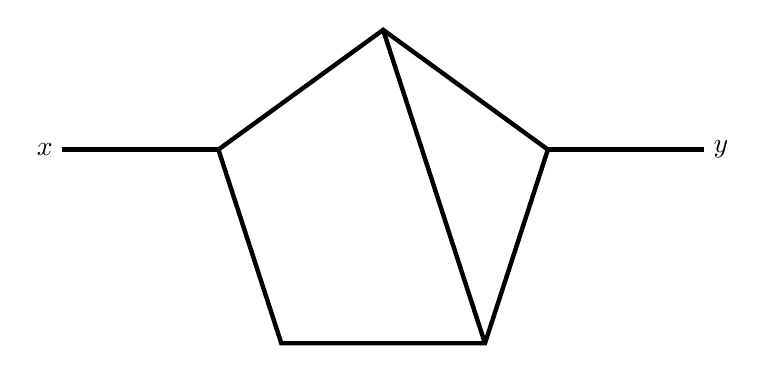
\begin{tikzpicture}[scale=2.2]%change the size here
	%pentagon
	\draw[ultra thick] (0,1)--(-0.9510565163,0.309017)--(-0.58778525229,-0.809017)--(0.58778525229,-0.809017)--(0.9510565163,0.309017)--cycle;
	%extra edges
	\draw[ultra thick] (0,1)--(0.58778525229,-0.809017);
	\draw[ultra thick] (-1.8510565163,0.309017)--(-0.9510565163,0.309017);
	\draw[ultra thick] (1.8510565163,0.309017)--(0.9510565163,0.309017);
	%label nodes   
	\node [left] at (-1.8510565163,0.309017) {$x$};
	\node [right] at (1.8510565163,0.309017) {$y$};
	\end{tikzpicture}
\end{center}

\begin{Exercise}[counter={sorszam}, difficulty=0]
	Azt mondjuk, hogy egy ir\'any\'itott %$G=(V,E)$
	gr\'af t\"om\"oren reprezent\'alt, ha adott egy $T$ Turing-g\'ep, ami $u,v$ bemenetre ki\'irja, hogy $uv$ \'el-e $\le n^k$ id\H oben, ahol $k$ egy fix konstans, pl.\ a feladat szempontj\'ab\'ol legyen $k=2$. A \la{Succinct-STconn} nyelv elemei azon $T$ Turing-g\'epek le\'ir\'asai, amik olyan gr\'afot t\"om\"or\'itenek, amiben van $st$ \'ut.\\
	a) Mutasd meg, hogy \PSPACE-ben eld\"onthet\H o \la{Succinct-STconn}.\\
	b) Mutasd meg, hogy \la{Succinct-STconn} \PSPACE-teljes.
\end{Exercise}	
\begin{Answer}
	a) \cl{NPSPACE}-beli \'es Savitch t\'etel.\\
	b) Az \'altal\'anos\'itott \'allapottere egy \PSPACE-es TG-nek pont egy ilyen gr\'afot ad.
\end{Answer}



\begin{Exercise}[counter={sorszam}, difficulty=2]
	a) A \la{Generalized Geography}-nak az a verzi\'oja is $\PSPACE$-teljes, ha a k\'et j\'at\'ekos k\"ul\"on-k\"ul\"on \'ep\'iti a saj\'at l\'anc\'at ugyanazon az ir\'any\'itott gr\'afon.
	(B\'armely cs\'ucsba csak egyik\"uk l\'ephet; mindkett\H onek meg van adva, hogy honnan kezd.)\\
	b) Ugyanez ir\'any\'itatlan gr\'afokra is $\PSPACE$-teljes.\\
	Mj.\ Azt nem tudom vizsg\'alt\'ak-e ezekben a verzi\'okban, hogy mi van, ha cs\'ucsokat szabad \'ujra haszn\'alni, csak az \'eleket nem.
\end{Exercise}	
\begin{Answer}
	Miltzow: Tron, a combinatorial Game on abstract Graphs \url{https://arxiv.org/abs/1110.3211} cikkben 13.~oldalt\'ol a), 15.\ oldalt\'ol b). (De egy\'ebk\'ent Nagy Kartal csin\'alt egyszer\H ubb megold\'ast r\'a.) 
\end{Answer}











\chapter{Véletlen algoritmusok}


\begin{Exercise}[counter={sorszam}, difficulty=-1]
	Adott egy $n$-edfokú polinom, és $n-1$ darab szám (nem feltétlen
	különbözőek). Ellenfelünk most azt állítja, hogy ennek a polinomnak
	multiplicitással éppen ezek a gyökei. Adjunk véletlent használó
	leleplező algoritmust, ami gyorsabb, mint a beszorzáson alapuló
	triviális determinisztikus eljárás.
\end{Exercise}


\begin{Exercise}[counter={sorszam}, difficulty=0]
	Adott egy \la{2-SAT} formula, amelyben minden klóz két különböző változót
	tartalmaz. \la{MAX2SAT}-nak nevezzük azt az optimalizálási feladatot, melynek célja
	a lehető legtöbb klózt igazzá tenni.
	\begin{enumerate}
		\item Adjunk gyors \emph{véletlen} algoritmust, amely nagy
		valószínűséggel olyan értékelést ad, amely a klózok legalább háromnegyedét
		igazzá teszi.
		\item Adjunk olyan determinisztikus polinomiális
		algoritmust, amely a klózok legalább háromnegyedét igazzá teszi.
	\end{enumerate}
\end{Exercise}

\begin{Exercise}[counter={sorszam}, difficulty=0]
	Hogyan tesztelhetj\"uk le gyorsan, hogy $q$ pr\'imhatv\'any-e?
\end{Exercise}	
\begin{Answer}
	Vegy\"uk $q$-nak az $i.$ gy\"ok\'et $i=1,\ldots,\log q$ \'ert\'ekekre \'es tesztelj\"uk mindr\H ol, hogy pr\'im-e.
	%max log q szamra kell tesztelni, hogy prim-e.
\end{Answer}

%\begin{Exercise}[counter={sorszam}, difficulty=-1]
%	Véges test felett vagyunk (bizonyos bonyodalmak elkerülése
%	végett). Adott három $n \times n$-es mátrix, $A,B,C$. Valaki azt állítja, hogy $AB=C$. Mi
%	ellenőrizni akarjuk ezt az állítást, úgy, hogy csak $O(n^2)$ szorzást végzünk,
%	de nem törekszünk teljes bizonyosságra: ha $AB \neq C$, akkor
%	$0.99$ valószínűséggel le akarjuk leplezni a csalást. Adjunk véletlen algoritmust
%	a feladatra.
%\end{Exercise}

\begin{Exercise}[counter={sorszam}, difficulty=0]
	Adj egy (RAM g\'epen) $\tilde O(n^2)$ idej\H u randomiz\'alt algoritmust, ami eld\"onti input $A,B,C$ $n\times n$-es eg\'esz m\'atrixokr\'ol, hogy $A\cdot B=C$ igaz-e. Melyik oszt\'alyban van ez az algoritmus \RP, \coRP \'es \BPP k\"oz\"ul?
\end{Exercise}	
\begin{Answer}
	$AB=C$ akkor \'es csak akkor, ha minden $x$-re $A(Bx)=Cx$, teh\'at ez val\'oj\'aban egy $n$ v\'altoz\'os line\'aris polinomazonoss\'ag tesztel\'es.
	Konkr\'etan egy v\'eletlen $x\in \{0,1\}^n$-re tesztelj\"uk, hogy $A(Bx)=Cx$ igaz-e.
	Ha $AB=C$, ez mindig teljes\"ul.
	K\"ulonben legyen $(AB)_{ij}\ne C_{ij}$.
	Ekkor csak egy $x_j$ \'ert\'ekre lesz $(A(Bx)_i=(Cx)_i$.
	Teh\'at legal\'abb $1/2$ es\'ellyel $A(Bx)\ne Cx$.
	Ez egy \coRP-beli algoritmus, teh\'at \BPP-beli is.
\end{Answer}

\begin{Exercise}[counter={sorszam}, difficulty=0]
	Az \Language nyelv eleme \RP-nek pontosan akkor, ha:
	
	Létezik egy olyan $p(n)$ polinom, és egy olyan \P-beli kétváltozós $M(x,y)$ reláció
	(olvasd: $y$ tanúja $x$-nek), hogy ha $x$ nem eleme \Language, akkor $x$-nek nincsen $p(|x|)$
	hosszú tanúja, ha $x$ eleme \Language, akkor viszont a $p(|x|)$ hosszú szavak legalább
	fele tanúja $x$-nek.
\end{Exercise}


\begin{Exercise}[counter={sorszam}, difficulty=0]
	Bizonyítsuk be, hogy az \RP definíciójában szereplő $1/2$-et tetszőleges
	$0<c<1$ konstansnak is választhattuk volna.
\end{Exercise}


\begin{Exercise}[counter={sorszam}, difficulty=0]
	Bizonyítsuk be, hogy a \BPP definíciójában szereplő $(1/3,2/3)$ helyett
	tetszőleges $(1/2-c,1/2+c)$ is állhatna, ahol $0<c<1/2$.
\end{Exercise}


\begin{Exercise}[counter={sorszam}, difficulty=-1]
	$\RP \subseteq \NP$, $\RP \subseteq \BPP$, $\cl{co-BPP} = \BPP$.
\end{Exercise}


\begin{Exercise}[counter={sorszam}, difficulty=0]
	Az \RP, \BPP, \ZPP nyelvosztályok mindegyike zárt a metszetre és unióra.
\end{Exercise}


\begin{Exercise}[counter={sorszam}, difficulty=0]
	\ZPP alábbi három definíciója ekvivalens:
	\begin{enumerate}
		\item Az algoritmus $1/2$-nél kisebb eséllyel passzolhat, és polinomiális futásidejű.
		\item Az algoritmus futásidejének várható értéke a bemenet hosszában polinomiális.
		\item $\RP \cap \cl{co-RP}$.
	\end{enumerate}
\end{Exercise}

\begin{Exercise}[counter={sorszam}, difficulty=0]
	$p(n)$ tetszőleges előre megadott polinom. \BPP definíciója ekvivalens mindkét alábbi
	definícióval: Létezik a nyelvhez olyan véletlen Turing-gép, amelynek tévedési valószínűsége
	\begin{enumerate}
		\item $2^{-p(n)}$ (erős \BPP definíció)
		\item $1/2-2^{-p(n)}$ (gyenge \BPP definíció)
	\end{enumerate}
\end{Exercise}


\begin{Exercise}[counter={sorszam}, difficulty=0]
	Mutasd meg p\'eld\'aul a \BPP -r\H ol, hogy ekvivalens defin\'ici\'okat kapunk, ha\\
	a) racion\'alis sz\'amok az eloszl\'asok (amik meghat\'arozz\'ak, hogy mikor merre l\'ep\"unk tov\'abb),\\
	b) csak egy darab \'allapot van, ami $1/2$--$1/2$ es\'ellyel l\'ep k\'et m\'asikba,\\
	c) van egy v\'eletlen szalagunk, melynek minden mez\H oje $1/2$ es\'ellyel 0 \'es 1,\\
	d) egy olyan p\'enzt ,,dob\'alhatunk'', ami valamilyen ismeretlen, konstans $p$ es\'ellyel lesz fej.\\
	e)~\hard Mutasd meg, hogyha az eloszl\'asr\'ol csak azt tessz\"uk fel, hogy rekurz\'iv,
	akkor $\BPP\not\subset \EXP$.
	\hint{ a) K\"ozel\'its\"uk a racion\'alis sz\'amokat diadikus racion\'alis sz\'amokkal az input hossz\'at\'ol f\"ugg\H o pontoss\'aggal. }
\end{Exercise}	
\begin{Answer}
	A b) az a) speci\'alis esete.\\
	Ha van egy a) t\'ipus\'u $T$ g\'ep\"unk, akkor abb\'ol \'ugy k\'esz\'ithet\"unk egy b) t\'ipus\'u $T'$-t, hogy ah\'anyszor randomiz\'alni kell, mindig le\'irjuk egy plusz szalagra, hogy \'eppen $T$ melyik \'allapot\'aban kell ezt megtenn\"unk, majd $T'$ egyetlen randomiz\'alt \'allapot\'aval addig sorsolunk, am\'ig el\'eg nagy pontoss\'aggal meg nem k\"ozel\'itj\"uk a racion\'alis sz\'amokat.
	A k\"ozel\'it\'es sz\"uks\'eges pontoss\'ag\'at, azaz azt, hogy a racion\'alis sz\'amot h\'any bin\'aris ``tizedes jegy'' pontoss\'agig sz\'amoljuk ki, az input hossza hat\'arozza meg.
	Ha $T$ $n^c$ id\H oben fut, akkor el\'eg $1/(2n^c)$ pontoss\'aggal k\"ozel\'iteni, \'igy az ebb\H ol ad\'od\'o hiba legfeljebb $(1-1/(2n^c))^{n^c}<1/e^2$, teh\'at az \"osszhiba legfeljebb $1/3+1/e^2<1/2$.
	Ez ism\'etl\'essel levihet\H o $1/3$ al\'a a szok\'asos m\'odon.\\
	A b) \'es c) ekvivalenci\'aja nyilv\'anval\'o.\\
	A d) speci\'alis esete a b)-c).\\
	Ha van egy b) t\'ipus\'u $T$ g\'ep\"unk, akkor abb\'ol \'ugy k\'esz\'ithet\"unk egy d) t\'ipus\'ut, hogy ah\'anyszor a randomiz\'al\'o \'allapotba l\'epn\'enk, dobjuk fel a p\'enzt k\'etszer.
	Ha fej-\'iras, l\'epj\"unk tov\'abb az egyik \'allapotba, ha \'iras-fej, akkor a m\'asikba, m\'ig ha k\'et azonos \'ert\'eket kapunk, akkor ism\'etelj\"uk ezt meg \'ujra.
	(Ha ezt olyan sokszor k\'ene megism\'etelni, hogy t\'ulmenn\'enk a megengedett fut\'asid\H on, akkor \'alljunk le, ennek \'ugyis kicsi az es\'elye.)\\
	e) Felismerhet\"unk egy olyan $L$ nyelvet, ami csak $x$ hossz\'at\'ol f\"ugg \'es annyira ritka, hogy csak $2^{2^t}$ alak\'u hossz\'us\'ag\'u szavak lehetnek $L$-ben.
	Azt, hogy $n$ benne van-e $L$-ben, ne lehessen \EXP-ben eld\"onteni, de $2^{2^n}$-ben m\'ar igen.
	Legyen egy \'allapot, amib\H ol $\sum_{n\in L} 1/n$ es\'ellyel l\'ep\"unk egy m\'asikba.
	\'Igy adott inputra kisebbekre meg tudjuk n\'ezni, hogy benne van-e, \'igy $n$ ism\'etl\'es ut\'an tudjuk, hogy kb.\ h\'any sikert v\'arunk, nagyobbak nem befoly\'asolj\'ak.
\end{Answer}

\begin{Exercise}[counter={sorszam}, difficulty=0]
	Eld\"onthetelen az \la{RP-ACCEPTANCE} nyelv, azaz, hogy egy le\'ir\'as\'aval adott randomiz\'alt, polinom id\H oben fut\'o Turing-g\'epr\H ol, hogy igaz-e, hogy
	minden $x$-et vagy legal\'abb $1/2$ es\'ellyel elfogad, vagy biztosan elutas\'it.
\end{Exercise}	
\begin{Answer}
	A meg\'all\'asi probl\'em\'at vezetj\"uk vissza.
	Input $T$-b\H ol k\'esz\'it\"unk egy $T'$-t, ami minden $x$ inputra $T$-t szimul\'alja a \"ures inputon $|x|$ l\'ep\'esig.
	Ha $T$ nem \'all le ezalatt, akkor $T'$ elutas\'it.
	Ha $T$ le\'all, akkor $T'$ fogadja el $|x|$-et $1/4$ es\'ellyel.
\end{Answer}


\begin{Exercise}[counter={sorszam}, difficulty=1]
	Egy adott konjunt\'iv norm\'alform\'ar\'ol valaki el\'arulja nek\"unk, hogy pontosan egy megold\'asa van (mint pl.\ egy Sudoku feladv\'anyn\'al). Mutassuk meg, hogy ha van polinomi\'alis algoritmus, ami megtal\'alja a megold\'ast, akkor $\RP=\NP$.	
\end{Exercise}	
\begin{Answer}
	Valiant-Vazirani t\'etel: \url{https://en.wikipedia.org/wiki/Valiant%E2%80%93Vazirani_theorem}.
	\end{Answer}

\begin{Exercise}[counter={sorszam}, difficulty=0]
	Ha \SAT eleme \BPP, akkor \SAT eleme \RP. (Ebből azonnal
	következik, hogy ha \NP része \BPP, akkor $\NP=\RP$. \wrk{Ennek prochat-nak kellene lennie, nem?})
\end{Exercise}


\begin{Exercise}[counter={sorszam}, difficulty=0]
	Érveljünk amellett, hogy $\DSPACE(O(n^{\log n}))$ nem része \BPP-nek. \wrk{Ezt a lecture05.ps-ben láttam, nem ismerem a megoldást.}
	
	\wrk{döm: szerintem ez nem nehéz, ha az alábbi megoldás jó.}
	
	\hint{Átlós módszer.}
\end{Exercise}

\sol{Felsoroljuk az összes véletlent használó Turing-gépet, mindet végtelen sokszor. Az $n$ hosszú inputokon az $n.$ Turing-gépet szimuláljuk addig, amíg $\le n^{\log n}$ tárat használ. Ha ezt bármikor túllépné, akkor leállunk. Mi nem tudunk véletlent használni, de sorban felírhatjuk az összes $n^{\log n}$ hosszú bitsorozatot, számoljuk, hogy melyikre mit outputolna a szimulált gép. (Ha több véletlen bitet használna, leállunk.) Végül pedig megnézzük, hogy mit outputolna többször és mi ennek az ellenkezőjét outputoljuk. Így biztos minden \BPP géptől eltértünk.}

\begin{Exercise}[counter={sorszam}, difficulty=0]
	\wrk{Yao tétele, kijelentve, hogy felhasználhatják Neumann minimax tételét.}
\end{Exercise}


\begin{Exercise}[counter={sorszam}, difficulty=0]
	Ha $\NP \neq \BPP$, akkor $\EXP \neq \cl{EXPSPACE}$.
\end{Exercise}




\begin{Exercise}[counter={sorszam}, difficulty=0]
	Legyen \PP azon nyelvek oszt\'alya, amikhez van minden inputra mindig polinomi\'alis id\H oben fut\'o randomiz\'alt Turing-g\'ep, ami $<1/2$ es\'ellyel hib\'azik.\\
	a) Mutasd meg, hogy $\NP \subseteq \cl{PP}$.\\
	b) $\cl{PP} \subseteq \PSPACE$.\\
	c) Mutasd meg, hogy ha a \PP -t v\'arhat\'o fut\'asid\H ovel defini\'aljuk, akkor
	az \'igy kapott oszt\'aly pontosan a rekurz\'iv nyelvek oszt\'alya lesz.
	\hint{ a) $\SAT\in\PP$, mert tippel\"unk egy tan\'ut, ha j\'o elfogadunk. Ha nem, akkor is elfogadunk $1/2-\eps$ es\'ellyel, valamint elutas\'itunk $1/2+\eps$ es\'ellyel. }
\end{Exercise}	
\begin{Answer}
	a) El\'eg azt bizony\'itani, hogy $\SAT\in\PP$.
	V\'alasszunk egy v\'eletlen \'ert\'ekad\'ast.
	Ha j\'o, akkor fogadjunk el.
	Ha nem j\'o, akkor is fogadjunk el $1/2-\eps$ es\'ellyel \'es utas\'itsunk el $1/2+\eps$ es\'ellyel.
	\'Igy ha $\Psi\notin \SAT$, akkor $>1/2$ es\'ellyel elutas\'itjuk, m\'ig ha $\Psi\in\SAT$, akkor legal\'abb $1/2^n+(1-1/2^n)(1/2-\eps)>1/2+1/2^{n+1}-\eps$ es\'ellyel elfogadjuk, teh\'at $\eps$-t v\'alaszthatjuk pl.\ $1/2^{n+2}$-nek.\\
	b) \PSPACE-ben v\'egig tudjuk sz\'amolni az \"osszes lehets\'eges fut\'asra az elfogad\'as val\'osz\'in\H us\'egek \"osszeg\'et.\\
	c) Ezek a Turing-g\'epek va\'oban csak rekuz\'iv nyelvet ismerhetnek fel, hiszen adott inputra addig sz\'amol\-gat\-hat\-juk, hogy mekkora es\'ellyel fogadnak/utas\'itanak el, am\'ig valamelyik $>1/2$ nem lesz.
	(Teh\'at a v\'arhat\'o fut\'asid\H ore nem is kell fels\H o korl\'at.)\\
	A rekurz\'iv nyelvek pedig val\'oban ebbe a csal\'adba tartoznak, hiszen el\'eg szimul\'alni egy, a nyelvet eld\"ont\H o Turing-g\'epet azzal a m\'odos\'it\'assal, hogy minden l\'ep\'es ut\'an $50\%$ es\'ellyel le\'allunk \'es v\'eletlenszer\H uen elfogadunk/elutas\'itunk.
	(Teh\'at a v\'arhat\'o fut\'asid\H o igaz\'ab\'ol lehet konstans is.)
	%http://cstheory.stackexchange.com/questions/8333/avarage-classes-for-pp-probabilistic-polynomial-time-and-ppt-machines-running/8425#8425
\end{Answer}


















\chapter{Polinomi\'alis hierarchia \'es or\'akulumok}

\section{Polinomi\'alis hierarchia}

\defi $\exists^p L := \left\{ x \in \{0,1\}^* \ \left| \ \left( \exists w \in \{0,1\}^{\leq p(|x|)} \right) \langle x,w \rangle \in L \right. \right\},$

\noindent
\'es hasonl\'oan $\forall^p L := \left\{ x \in \{0,1\}^* \ \left| \ \left( \forall w \in \{0,1\}^{\leq p(|x|)} \right) \langle x,w \rangle \in L \right. \right\}.$

\noindent
Ezekkel a jelölésekkel $\NP=\cl{\exists\cdot \P}$ és $\coNP=\cl{\forall\cdot \P}$. Ezen felbuzdulva $\Sigmak:=\cl{\exists\cdot\forall\cdot\exists\ldots \P}$ és $\Pik:=\cl{\forall\cdot\exists\cdot\forall\ldots \P}$, ahol összesen $k$ db kvantor áll a $\P$ el\H ott. Teh\'at ezekkel a jelölésekkel $\NP=\Sigmaone$ és $\coNP=\Pione$.
A polinomi\'alis hierarchia $\PH:=\cup \Sigmak$.
%Szint\'en elterjedt az $\MA=\cl{\exists\cdot \BPP}$ jel\"ol\'es.
%nem is uaz: https://complexityzoo.uwaterloo.ca/Complexity_Zoo:E#existsbpp

\begin{Exercise}[counter={sorszam}, difficulty=0]
	$\Sigmak\subset \Sigmakplus\cap\Pikplus$.
\end{Exercise}

\begin{Exercise}[counter={sorszam}, difficulty=0]
	$\Sigmak\subset\PSPACE$.
\end{Exercise}	

\begin{Exercise}[counter={sorszam}, difficulty=0]
	$\Pik\subset\Sigmak \Rightarrow \Sigmak=\PH$.
\end{Exercise}	

\begin{Exercise}[counter={sorszam}, difficulty=-1]
	Ha létezik \PH-teljes nyelv, akkor összeomlik a polinomiális hierarchia.
\end{Exercise}

\sol{ Tegyük fel, hogy létezik \PH-teljes nyelv, méghozzá a hierarchia $k$-dik szintjén lévő $L$ nyelv. Ekkor a hierarchia magasabb szintjein álló nyelvek visszavezethetőek rá, és \wrk{blabla kezdek teljesen elálmosodni}. }

\begin{Exercise}[counter={sorszam}, difficulty=0]
	Ha $\PH=\PSPACE$, akkor a hierarchiának csak véges sok szintje van.
	\hint{ El\H oz\H o miatt. }
\end{Exercise}


\begin{Exercise}[counter={sorszam}, difficulty=0]
	Tegy\"uk fel, hogy adva van egy konjukt\'iv norm\'al forma, melynek v\'altoz\'oi $x_i$-k \'es $y_i$-k. Azt szeretn\'enk eld\"onteni, hogy minden $x_i$ behelyettes\'it\'esre van-e az $y_i$-knek olyan behelyettes\'it\'ese, ami kiel\'eg\'it\H o. Mutassuk meg, hogy ez $\Pitwo$-ben van. Mi lenne, ha az lenne a k\'erd\'es, hogy van-e $x_i$, hogy minden $y_i$-re igaz a formula?
\end{Exercise}	 
\begin{Answer}
	Akkor trivin \Sigmatwo-ban lenne, de az is igaz, hogy \NP-beli, mert azt k\"onny\H u ellen\H orizni, hogy egy KNF-et minden \'ert\'ekad\'as igazz\'a tesz-e.
\end{Answer}

\begin{Exercise}[counter={sorszam}, difficulty=0]
	Legyen $L$ az $n^2\times n^2$ m\'eret\H u olyan \'altal\'anos\'itott Sudoku \'all\'asok nyelve, ahol ak\'arhova be\'irunk egy sz\'amot (nem azonos sorba/oszlopba/n\'egyzetbe egy ugyanolyan sz\'ammal), marad megold\'asa.\\
	a) Melyik oszt\'alyban van $L$?\\
	b) Nincs benne egy kisebben is?
\end{Exercise}	
\begin{Answer}
	\Pitwo-ban van trivi, de igaz\'ab\'ol \Sigmaone-ben is, mert az \"osszes lehet\H os\'eget leellen\H orizhetj\"uk.
\end{Answer}

\begin{Exercise}[counter={sorszam}, difficulty=1]
	$\NP \subset \Ppoly \Rightarrow \Sigmatwo=\PH$.
\end{Exercise}	
\begin{Answer}
	Karp-Lipton t\'etel.\\
	\"Otlet: El\H oször mutassuk meg, hogy ekkor olyan hálózat is van, ami minden kielégíthet\H o \SAT formulához ad egy helyes kiértékelést. Aztán mutassuk meg, hogy \"osszeomlana a polinomi\'alis hierarchia.
	
	Ha $\NP \subset \Ppoly$, akkor van egy $p(n)$ poly hossz\'u bitsorozat \'es $T$ TG, hogy $T(\Psi,p(n))=1$ akkor \'es csak akkor ha $\Psi\in\SAT$. S\H ot, olyan $T$ is van, hogy $T(\Psi,p(n))=1$ eset\'en m\'eg ki is ad egy $x$-et, amire $\Psi(x)$ igaz. Most azt fogjuk megmutatni, hogy $\Pitwo\subset\Sigmatwo$, ebb\H ol k\"ovetkezik az \'allit\'as. Legyen $L\in \Pitwo$. Ekkor $\Psi\in L$ akkor \'es csak akkor, ha minden $z$-re $\Psi_z\in \SAT$, valami \P-beli $\Psi_z$-re. De ez ekvivalens azzal, hogy $\exists p(n) \forall z T(\Psi_z,p(n))=1$ \'es $\Psi_z(x_z)$ igaz, ahol az $x_z$-t is $T$ adja ki.
\end{Answer}

\begin{Exercise}[counter={sorszam}, difficulty=1]
	$\EXP\subset \Ppoly \Rightarrow \EXP= \Sigmatwo$.
\end{Exercise}	
\begin{Answer}
	Meyer t\'etele (de Karp-Lipton cikkben van).\\
	El\H oz\H oh\"oz hasonl\'oan. Lenne egy hálózat, ami egy \EXP-es sz\'am\'it\'as b\'armelyik hely\'en, b\'armikor felvett \'ert\'eket meg tudn\'a mondani. Egy ilyennek a helyess\'eg\'et ellen\H orizni is tudjuk \coNP-ben.
	%forras: vargadanis
\end{Answer}

\begin{Exercise}[counter={sorszam}, difficulty=0]
	Tegyük fel, hogy adott egy játék, ahol két játékos felváltva lép és egy $poly(n)$ méret\H u táblán játszanak \'ugy, hogy felv\'altva elfoglalnak egy mez\H ot (pl.\ am\H oba). Az állás alapján mindig el lehet dönteni \P-ben, hogy nyert-e valaki. Tegy\"uk fel, hogy a játék $k$ lépés alatt garant\'altan véget ér. Mutassuk meg, hogy azon \'all\'asok nyelve, amikre kezd\H onek van nyer\H o stratégiája $\in \Sigmak$. S\H ot.
\end{Exercise}	
\begin{Answer}
	S\H ot (Borb\'enyi M\'arton), \P-beli, mert csak ennyi opci\'o van konstans k\"or\"os j\'at\'ekban \'es mindet v\'egign\'ezhetj\"uk.
	Ha a t\'abla exp m\'eret\H u lenne vagy k\"or\"onk\'ent $n$-et rakn\'anak, akkor csak \Sigmak-t tudn\'ank bizony\'itani.	
\end{Answer}

\begin{Exercise}[counter={sorszam}, difficulty=0]
	Igaz-e, hogy ,,G-ben pontosan $k$ méretű a legnagyobb klikk?'' eleme \Sigmatwo?
\end{Exercise}

\begin{Exercise}[counter={sorszam}, difficulty=1]
	Bizonyítsuk be, hogy \cl{\Sigma_4} nem része a $\SIZE(n^t)$ nemuniform bonyolultsági
	osztálynak, semmilyen fix $t$-re. \wrk{SIZE definiálandó? Ha igen, hol?}
	
	\hint{ Az alternációt használjuk fel arra, hogy tippeljünk egy nagy bonyolultságú Boole-függvényt, és ellenőrizzünk is le. }
\end{Exercise}

\begin{Exercise}[counter={sorszam}, difficulty=1]
	Az előző feladat és a Karp-Lipton tétel alkalmazásával lássuk be, hogy az
	előző feladat állítása \cl{\Sigma_4} helyett \Sigmatwo-vel is igaz.
	
	\hint{ Alkalmazzunk esetszétválasztást aszerint, hogy $\SAT \in \SIZE(n^t)$ \wrk{befejezetlen}. }
\end{Exercise}

\begin{Exercise}[counter={sorszam}, difficulty=0]
	A \la{MIN-DNF} nyelv párokból áll. A pár első tagja egy $\phi$ DNF formula. A második egy $k$ egész szám.
	A pár akkor van benne \la{MIN-DNF}-ben, ha létezik $k$-nál nem hosszabb $\psi$ formula, amely ekvivalens $\phi$-vel.
	Bizonyítsuk be, hogy \la{MIN-DNF} eleme \Sigmatwo.
\end{Exercise}

\section{Or\'akulumok}

\defi Az {\em orákulumos} Turing-gép egy többszalagos $M^?$ Turing-gép, melynek egyik szalagja a kitüntetett kérdez\H o-szalag. Az orákulum egy tetsz\H oleges $A$ nyelv lehet. $M^?$-nek van egy speciális $q_?$ állapota. Ha ebbe kerül, akkor az orákulum válaszol neki, hogy az éppen akkor a speciális szalagján lev\H o szó benne van-e az $A$ nyelvben. 

Az $x$ bemenethez tartozó kimenetet $M^A(x)$-szel jelöljük. Ha $\XP$ egy olyan nyelv, ami Turing-gépek egy speci\'alis családj\'aval van defini\'alva, akkor $\XP^A$ jelöli azokat az $L$ nyelveket, amihez van ebb\H ol a csal\'adb\'ol Turing-g\'ep, amihez $A$ orákulumot adva $L$-et ismeri fel. Ha valamely bonyolults\'agi oszt\'alyhoz van teljes nyelv, akkor gyakran a bonyolults\'agi oszt\'alyt \'irjuk a kitev\H obe, pl. $\P^{\NP}$ azt jelenti, hogy $\P^{\SAT}$. Ha nincs teljes nyelv, akkor is \'irhatunk bonyolults\'agi oszt\'alyt a kitev\H obe, ekkor az \'uj oszt\'aly az \"osszes lehets\'eges nyelv uni\'oja, pl.\ $\P^{\BPP}=\cup \{\P^{L}\mid {L\in \BPP}\}$.

\begin{Exercise}[counter={sorszam}, difficulty=0]
	Legyen $A$ egy $\P$-beli nyelv. Mutassuk meg, hogy $\P^A=\P$.
\end{Exercise}	
\begin{Answer}
	Futassuk magunk az $A$-t eld\"ont\H o TG-et ahelyett, hogy k\'erdezn\'enk t\H ole.
\end{Answer}


\begin{Exercise}[counter={sorszam}, difficulty=0]
	$\P^{\NP}=\P^{\SAT}$.
\end{Exercise}	
\begin{Answer}
	Minden \NP-beli nyelv visszavezethet\H o \SAT-ra, \'es azt\'an mint el\H oz\H o.
\end{Answer}


\begin{Exercise}[counter={sorszam}, difficulty=0]
	Ha $\E=\DTIME(2^{O(n)})$, akkor mi lesz $\P^{\E}$?
\end{Exercise}	
\begin{Answer}
	\EXP.
\end{Answer}

\begin{Exercise}[counter={sorszam}, difficulty=0]
	$\EXP^{\EXP} = \cl{EEXP}$. ($\cl{EEXP} = \DTIME(2^{2^{n^c}})$.)
\end{Exercise}


\begin{Exercise}[counter={sorszam}, difficulty=0]
	$\PSPACE^{\PSPACE}=\PSPACE$.
\end{Exercise}	
%\begin{Answer}
%\end{Answer}


\begin{Exercise}[counter={sorszam}, difficulty=0]
	Mutasd meg, hogy $\NP\cup \coNP\subset \P^{\NP}$.
\end{Exercise}	
\begin{Answer}
	$\NP\subset \P^{\NP}$ nyilv\'anval\'o \'es $\P^{\NP}$ z\'art komplementerre.
\end{Answer}


\begin{Exercise}[counter={sorszam}, difficulty=0]
	$\NP^{\NP\cap \coNP}= \NP$.
\end{Exercise}	
\begin{Answer}
	B\'armit k\'erdezn\'enk, megtippelhetj\"uk r\'a a v\'alaszt \'es tal\'alhatunk r\'a tan\'ut magunk.\\
	Forr\'as: \url{http://blog.computationalcomplexity.org/2017/03/np-in-zpp-implies-ph-in-zpp.html} alapj\'an.
\end{Answer}


\begin{Exercise}[counter={sorszam}, difficulty=0]
	$\NP^{\NP}= \Sigmatwo$.
\end{Exercise}	
\begin{Answer}
	$\NP^{\NP}\supset \Sigmatwo$ defin\'ici\'o szerint.
	$\NP^{\NP}\subset \Sigmatwo$-hez tippelj\"uk meg \"osszes k\'erd\'esre v\'alaszokat, amire van tan\'u, tippelj\"uk meg, amire nincs, azokra meg ez egyetlen $\Pione$-beli mondat, hogy egyikhez sincs.
\end{Answer}

\begin{Exercise}[counter={sorszam}, difficulty=1]
	$\BPP^{\BPP}=\BPP$.
	\hint{ Az or\'akulum nyelvhez van $\BPP$ algoritmus, ami $<1/2^n$ es\'ellyel hib\'azik. Ha ezt futtatjuk r\'a, akkor annak az es\'elye, hogy valaha is hib\'azunk k\'erdez\'es szimul\'al\'asakor kicsi. }
\end{Exercise}	
\begin{Answer}
	Legyen or\'akulumos TG fut\'asideje $n^k$ \'es hib\'azzon $<1/8$ es\'ellyel.
	Or\'akulum nyelvhez minden $n$-re \'es $k$-re van \BPP alg, ami $<1/(8n^k)$ es\'ellyel hib\'azik.
	Ez ism\'etelget\'essel kaphat\'o b\'armelyik \BPP-sb\H ol, teh\'at tudjuk is szimul\'alni $poly(n^k)$ id\H oben.
	Ha mindig ezt futtatjuk k\'erdez\'es helyett, akkor annak az es\'elye, hogy valaha is hib\'azunk k\'erdeze\'s szimul\'al\'asakor $<1/8$, teh\'at az \"osszhiba $<1/4$.
\end{Answer}

\begin{Exercise}[counter={sorszam}, difficulty=0]
	Igaz vajon, hogy $\RP^{\RP}=\RP$?	
\end{Exercise}	
\begin{Answer}
	$\coRP\subset \RP^{\RP}$, sz\'oval k\"ovetkezne bel\H ole $\coRP=\RP$, jelenleg nem ismert.
\end{Answer}

\begin{Exercise}[counter={sorszam}, difficulty=1]
	$\NP^{\BPP} \subseteq \BPP^{\NP}$.
\end{Exercise}

\begin{Exercise}[counter={sorszam}, difficulty=0]
	$\BPP \subseteq \ZPP^{\NP}$.
	
	\hint{ $\cl{pBPP}=\cl{pRP}^{\cl{pRP}}$. \wrk{opg5.ps} }
\end{Exercise}

\begin{Exercise}[counter={sorszam}, difficulty=0]
	Egy v\'eletlen $R$ nyelvre egy val\'osz\'in\H us\'eggel $\BPP\subsetneq \P^R$.	
\end{Exercise}	
\begin{Answer}
	Forr\'as: Charles H. Bennett, John Gill: Relative to a Random Oracle... \url{https://doi:10.1137/0210008}\\
	Ha $L\in \BPP$, akkor olyan Random TG is van, ami az \"osszes inputra \"osszesen $<1\%$-ot hib\'azik. Ezzel meg tudjuk mutatni, hogy a v\'eletlen nyelvek $99\%$-a tartalmazza $\BPP$-t, teh\'at egy val\'osz\'in\H us\'eggel $\BPP\subset \P^L$. Viszont egy val\'osz\'in\H us\'eggel $L \notin \BPP$, teh\'at egy val\'osz\'in\H us\'eggel $\BPP\ne \P^L$.
\end{Answer}

\begin{Exercise}[counter={sorszam}, difficulty=0]
	Mutass olyan $\XP$ bonyolults\'agi oszt\'alyt, amire $\XP^{\XP}\ne \XP$.
\end{Exercise}	
\begin{Answer}
	I. $\E$ vagy $\EXP$ j\'o id\H ohierarchia miatt.\\
	II. (Csern\'ak Tam\'as) Rekurz\'iv felsorolhat\'ok is j\'ok, mert nem z\'artak komplementerre.
\end{Answer}


\begin{Exercise}[counter={sorszam}, difficulty=0]
	$\exists A: \P^A= \NP^A$.
\end{Exercise}	
\begin{Answer}
	I. Ha $A$ \PSPACE-teljes, ez Savitch t\'etel.\\
	II. (\'Agoston P\'eter) $A=\PH$, mert ha nemdet $k$. szintr\H ol k\'erdez, det k\'erdezhet a $(k+1)$-edikr\H ol.
\end{Answer}


\begin{Exercise}[counter={sorszam}, difficulty=1]
	$\exists A: \P^A\ne \NP^A$.
\end{Exercise}	
\begin{Answer}
	Nyelv legyen, hogy van-e $A$-ban az inputtal megegyez\H o hossz\'us\'ag\'u string.
	Meg lehet csin\'alni \'atl\'os m\'odszerrel, hogy minden $\P$-belit\H ol k\"ul\"onb\"ozz\"on.
\end{Answer}


\begin{Exercise}[counter={sorszam}, difficulty=1]
	Van $A$ nyelv, hogy minden $L\in \NEXP^A$-hoz van $S\subset \N$ v\'egtelen halmaz \'es $L'\in\NP^A$, amire $L|_S=L'|_S$.
\end{Exercise}	
\begin{Answer}
	Forr\'as: Buhrman, Fortnow, Santhanam: Unconditional Lower Bounds Against Advice \url{https://doi.org/10.1007/978-3-642-02927-1_18}.
\end{Answer}














\chapter{H\'al\'ozatok}

\section{Általános Boole-hálózatok}

\begin{Exercise}[counter={sorszam}, difficulty=0]
	A méret polinomiális mértékű megnövelése árán elérhető, hogy az $AND,OR,NOT$ hálózat
	összes $NOT$ kapuja a legalsó szinten legyen.
\end{Exercise}


\begin{Exercise}[counter={sorszam}, difficulty=0]
	\begin{enumerate}
		\item Mely Boole-függvények számíthatóak ki Boole-hálózattal?
		\item Milyen $f(n)$-re igaz, hogy ekkora hálózat már minden $n$-változós Boole-függvényhez létezik?
	\end{enumerate}
\end{Exercise}


\begin{Exercise}[counter={sorszam}, difficulty=0]
	\begin{enumerate}
		\item Mely monoton Boole-függvények számíthatóak ki monoton Boole-hálózattal?
		\item Milyen $f(n)$-re igaz, hogy ekkora monoton hálózat már minden $n$-változós
		monoton Boole-függvényhez létezik?
	\end{enumerate}
\end{Exercise}


\begin{Exercise}[counter={sorszam}, difficulty=0]
	Adjunk $O(n \log n)$ méretű Boole-hálózatot a \la{MAJORITY} függvényre.
\end{Exercise}


\begin{Exercise}[counter={sorszam}, difficulty=1]
	Adjunk $O(n)$ méretű Boole-hálózatot a \la{MAJORITY} függvényre.
	
	\hint{ \wrk{Igaz-e az, hogy a bináris fát alkotó ismételt összeadással $\Sigma_i O(i)n/2^i = O(n)$ méretben vagyunk? Ha igen, akkor nem is nehéz.} }
\end{Exercise}


\begin{Exercise}[counter={sorszam}, difficulty=2]
	Ha \NP része \cl{P/log}, akkor $\P = \NP$.
	
	\hint{ Vegyük észre, hogy egy adott bemenetre egy adott \cl{P/log} algoritmust le tudunk futtatni minden egyes logaritmikus hosszúságú tanáccsal, polinomiális futásidőben maradva. De sajnos nincsen nyilvánvaló eljárás, amely eldönti, hogy a végigpróbálgatott tanácsok közül melyik a helyes. }
	
	\hint{ Azt kihasználva, hogy a \SAT eldöntési feladat $\cl{P/log}$-ban van, adjunk polinomidejű eljárást, amely megoldja a \SAT keresési feladatot. Az eljárásnak ne legyen bemenete a logaritmikus hosszúságú tanács, csak használja ki annak létezését. }
\end{Exercise}


\begin{Exercise}[counter={sorszam}, difficulty=2]
	Adjunk \PSPACE-beli nyelvet, amelynek az általános Boole-hálózat bonyolultsága
	$O( {n^3} / {\log n} )$ és $O(n^3)$ közé esik.
	
	\hint{ Először oldjuk meg a feladatot úgy, hogy elhagyjuk a \PSPACE-beliség feltételét, aztán adjunk \PSPACE-beli algoritmust a megtalált nyelvre. }
	
	\hint{ Az adott hálózati bonyolultságú nyelv megtalálásához először tekintsünk egy olyan nyelvet, amelynek a bonyolultsága $2^n/{3n}$ és $2^n$ közé esik. Ilyen nyelv Shannon tétele szerint létezik. Alkalmazzunk párnázást. \wrk{Tényleg ilyen jó konstanst ad Shannon tétele úgy, ahogy azt mi tanuljuk?} }
	
	\hint{ Ha egyáltalán létezik olyan nyelv, amelynek az általános Boole-hálózat bonyolultsága $c_2 {n^3} / {\log n}$ és $c_1 n^3$ közé esik, akkor ilyen nyelvet \PSPACE (konkrétan $\DSPACE(n^3)$) algoritmussal is tudunk találni: Sorban haladjunk végig a $c_1 n^3$ méretű hálózatokon. Álljunk meg, ha olyat találunk, amelynek egyetlen $c_2 {n^3} / {\log n}$ méretű hálózattal sem egyezik meg az igazságtáblája. A megtalált hálózatot értékeljük ki a bemenetünkön. }
	
	\hint{ Élesebb megoldás az első hintre: Jelöljük az $n^3-n-1$ méretű hálózatokkal kiszámítható $n$-változós Boole-függvények halmazát $F_n$-nel. Ez a halmaz nem üres, és nem esik egybe az összes $n$-változós Boole-függvények halmazával. Léteznek tehát olyan $f \in F_n$, $g \notin F_n$ $n$-változós Boole-függvények, amelyek csak egyetlen $a$ bemeneten különböznek. $g(x)=(x=a) \vee f(x)$ vagy $g(x)=(x=a) \vee f(x)$, tehát $g$ is kiszámítható legfeljebb $(n^3-n-1)+n+1=n^3$ méretű hálózattal. }
	
	\wrk{Mindezt midterm-sol.ps-ból loptam, jelölésestül, úgyhogy majd kreditet kell adni Luca Trevisan-nak. Az élesebb megoldást feladattá lehetne különíteni.}
\end{Exercise}


\begin{Exercise}[counter={sorszam}, difficulty=0]
	Bizonyítsuk be, hogy a monoton Boole-hálózatok kiértékelési feladata \P-teljes. \wrk{Melyik redukcióra?}
\end{Exercise}

\sol{ A nemtriviális irányhoz visszavezetjük a feladatra az általános Boole-hálózatok kiértékelési feladatát. A visszavezetés triviális, ha az általános Boole-hálózatainkat úgy definiáltuk, hogy csak a legalsó szintjén engedünk meg tagadó kapukat. Ekkor egyszerűen minden negált változóhoz felveszünk egy új változót, megkettőzve a változók számát, és monotonná téve a hálózatot. Ha az általános Boole-hálózatainknak magasabb szintjein is megengedünk tagadó kapukat, akkor ennek a triviális visszavezetésnek az alkalmazása előtt el kell végeznünk azt a polinom idejű átalakítást, amely a tagadó kapukat ,,lenyomja'' a hálózat legalsó szintjére. \wrk{Ez csak akkor elég részletes, ha ezt a lenyomást le tudom hivatkozni egy másik feladatba.}
}


\begin{Exercise}[counter={sorszam}, difficulty=0]
	Bizonyítsuk be, hogy a stratified Boole-hálózatok kiértékelési feladata \NL-teljes.
	Stratified-nak hívunk egy Boole-hálózatot, ha vagy csupa $AND$, vagy csupa $OR$ kaput tartalmaz.
\end{Exercise}


\begin{Exercise}[counter={sorszam}, difficulty=-1]
	Egy nyelv ritka, ha $n$ betűs szavainak száma $poly(n)$. A ritka nyelvek osztályát \SPARSE jelöli. \P-közelinek nevezünk egy \Language nyelvet, ha valamely $\Language' \in \P$ nyelvvel vett szimmetrikus differenciája ritka. \cl{P-close} a \P-közeli nyelvek osztálya. Bizonyítsuk be, hogy \cl{P-close} valódi része \Ppoly-nak.
	
	\hint{ Része, hiszen a szimmetrikus differencia belekódolható a tanácsba. A tartalmazás valódiságának bizonyításához tekintsük természetes számok egy nemrekurzív $H$ halmazát. Legyen $x \in \Language$ akkor és csakis akkor, ha $|x| \in H$. Ez az \Language nyelv \Ppoly, de nem \cl{P-close}. }
\end{Exercise}


\begin{Exercise}[counter={sorszam}, difficulty=1]
	Létezik olyan nyelv \PH-ban, amely nincs benne $\SIZE(O(n))$ -ben.
	
	\hint{ Ha \SAT egy ilyen nyelv, akkor készen vagyunk, tehát a megoldáshoz feltehetjük, hogy \SAT-ra létezik lineáris méretű hálózat-sorozat. }
\end{Exercise}


\begin{Exercise}[counter={sorszam}, difficulty=2]
	(Kannan tétele) Bizonyítsuk be a fenti állítást \PH helyett a $\Sigmatwo \cap \cl{\Pi_2}$ osztállyal.
\end{Exercise}

\sol{ \wrk{Nem tudom, hogy hol a megoldás, de Kannan-é az eredmény, és írnak róla itt: http://citeseer.ist.psu.edu/594507.html} }

\begin{Exercise}[counter={sorszam}, difficulty=-1]
	Ha $\NP \subseteq \SIZE(O(n))$, akkor $\P \neq \NP$. Használjuk fel Kannan tételét.
\end{Exercise}



%------------------------------

\section{Kis mélységű Boole-hálózatok}

\begin{Exercise}[counter={sorszam}, difficulty=0]
	\begin{enumerate}
		\item Adjunk alsó és felső becslést az $n$-változós \la{PARITY} függvényt kiszámító 2 mélységű Boole-hálózat méretére.
		\item Adjunk felső becslést az $n$-változós \la{PARITY} függvényt kiszámító 3 mélységű Boole-hálózat méretére.
	\end{enumerate}
\end{Exercise}


\begin{Exercise}[counter={sorszam}, difficulty=0]
	\begin{enumerate}
		\item Mutassunk lineáris méretű hálózatot, amelynek bemenete két
		$n$ bit hosszú szám, kimenete a két szám ($n+1$ bit hosszú) összege.
		(Minden kettes számrendszerben történik.)
		\item Az $x \geq y$ (más néven $\la{COMPARE}(x,y)$) reláció \ACnull-ban van.
		\item Az összeadás \ACnull-ban van.
		\item \hard Mekkora lehet egy \ACnull összeadó hálózat konstans mélysége?
	\end{enumerate}
\end{Exercise}


\begin{Exercise}[counter={sorszam}, difficulty=0]
	\wrk{Ugyanolyan nehéz az n darab n bites szám rendezése, mint az n darab egybitesé. Ugye ez igaz?}
\end{Exercise}


\begin{Exercise}[counter={sorszam}, difficulty=0]
	Tudjuk, hogy \la{PARITY} nem eleme \ACnull. Bizonyítsuk be, hogy
	\begin{enumerate}
		\item \la{MAJORITY} sem.
		\item \la{SORT} sem.
		\item $\la{MULTIPLY}(x,y)$ sem.
		\item $\la{DIVIDE}(x,y)=[x/y]$ sem.
	\end{enumerate}
\end{Exercise}


\begin{Exercise}[counter={sorszam}, difficulty=0]
	Most azt tudjuk, hogy \la{MULTIPLY} nem eleme \ACnull. Bizonyítsuk be, hogy \la{DIVIDE} sem.
\end{Exercise}


\begin{Exercise}[counter={sorszam}, difficulty=0]
	\la{PARITY} eleme \cl{TC^0}.
\end{Exercise}


\begin{Exercise}[counter={sorszam}, difficulty=2]
	\la{MAJORITY} eleme \cl{NC^1}.
\end{Exercise}

\sol{ \wrk{Az alábbiakban csak ész nélkül beegereztem Németh András megoldását. Megfésülendő, köszönetnyilvánítandó.}
	
	A MAJORITY kiszámítására a triviális technikát lenne jó alkalmazni:
	kiszámítjuk valahogy egy hálózattal a bitek első felén az egyesek
	számát, ill. ezzel párhuzamosan a bitek második felén, ezeket
	ábrázoljuk bináris számként, majd összaadjuk, és a kapott bináris
	számot összahasonlítjuk $n/2$-vel. A bitek első felén az egyesek
	számát természetesen rekurzívan akarjuk számítani: a bitek első
	negyedén levő egyesek száma és a bitek második negyedén levő egyesek
	száma összegeként. És így tovább, egyre kisebb számokat kell
	összeadnunk.
	
	Ez persze így bár helyes hálózatot eredményez, de mégsem oldja meg a
	feladatot, mert a hálózat túl mély lesz. Két $n$-bites szám
	összeadására ugyanis a triviális esetben cn mély hálózatot építenénk
	(általános iskolás összeadás hálósítása), így pl. $n=2^k$ esetén
	összesen $1+2+3+...+k=O(k^2)=O(\log^2(n))$ mély hálóra lenne
	szükségünk. Valójában létezik módszer k bites számok $O(\log k)$
	párhuzamos időben történő összeadására, de nekünk még ez sem lenne
	elég (ha jól sejtem ez $O(\log n\log\log n)$-et adna közvetlenül
	használva), de ennek a módszernek az egyik alapötletét fogjuk
	használni.
	
	Ábrázoljuk minden lépésben az adott szakaszokon található egyesek
	számát kiegyensúlyozott (pl.) négyes számrendszerbeli számként, azaz
	$\sum_{i=0}^k 4^ia_i$ alakban, ahol $a_i \in
	\{-3,-2,-1,0,1,2,3\}=:J$. Ez az ábrázolás persze nem egyértelmű, de
	sebaj. Két ilyen számot konstans mély hálózattal össze lehet adni.
	Könnyen elenőrizhető ugyanis, hogy ha $x,y \in J$, akkor $x+y$
	felírható $4a+b$ alakban, ahol $a \in {-1,0,1}$ és $b \in
	\{-2,-1,0,1,2\}$. Ez a felírás nyilván elvégezhető egy konstans
	méretű $E$ hálóval. Ha tehét két $n$ jegyű számot akarok összeadni,
	akkor egyszerre alkalmazom $E$-t az összes azonos helyiértékű
	számjegypárra, majd az $a$-ba kerülő helyiértéket hozzáadom a
	következő helyiértéken számított $b$-hez, ami a $b$-re és $a$-ra
	tett megkötés miatt már nem képez maradékot. Ezt az összeadást
	alkalmazva az első bekezdésben leírt módon egy $O(\log n)$ mélységű
	hálózattal ki tudom számítani az egyesek számát, amit egy
	kiegyensúlyozott, $O(\log n)$ jegyű négyes számrendszerbeli számként
	kapok meg. Ezt egy újabb $O(\log n)$ méretű hálózattal akár a
	triviális módon, a legkisebb helyiértéktől indulva standard alakra
	hozhatjuk. (Ehhez mindössze annyit kell észrevenni, hogy egy szám
	mod $4^k$ maradéka csak az utolsó $k$ számjegytől függ
	kiegyensúlyozott alakban is.) Még ugyanilyen mélységet igényel az
	összehasonlítás, így sikerült igazolni, hogy $MAJORITY \in NC^1$
	(Az, hogy az alkalmazott kapuk száma polinomiális $n$-ben, az
	triviális.)
	
	Megjegyzés: Egy $k$ jegyű kiegyensúlyozott szám valójában $O(\log k)$
	párhuzamos időben is standard alakra hozható, így áll össze az
	$O(\log k)$ párhuzamos idejű összeadás.
}


\begin{Exercise}[counter={sorszam}, difficulty=0]
	\la{SORT} eleme monoton \cl{AC^1}.
\end{Exercise}


\begin{Exercise}[counter={sorszam}, difficulty=1]
	A reguláris nyelvek \cl{NC^1}-ben vannak.
\end{Exercise}


\begin{Exercise}[counter={sorszam}, difficulty=0]
	$n$ darab $n$-bites szám összeadása \cl{TC^0}-ban van.
\end{Exercise}


\begin{Exercise}[counter={sorszam}, difficulty=0]
	$\la{MULTIPLY}(x,y)$ eleme $AC^1$. \wrk{Sőt, \cl{TC^0}-nak is eleme, ugye?}
\end{Exercise}


\begin{Exercise}[counter={sorszam}, difficulty=0]
	$n$ darab $n$-bites szám rendezése \cl{TC^0}-ban van.
	
	\hint{ Vegyük a páronkénti összehasonlításaikat. }
\end{Exercise}


\begin{Exercise}[counter={sorszam}, difficulty=0]
	Borogyin tétele: $\cl{NC^1} \subseteq \LOGSPACE$.
	
	\hint{ \wrk{(Du-Ko 6.24.) Először végezzünk el egy \LOGSPACE transzformációt, amely az adott bemeneti hálózatot formulává alakítja. Aztán értékeljük ki a formulát. Szétszedendő több feladatra.} }
\end{Exercise}


\begin{Exercise}[counter={sorszam}, difficulty=0]
	\begin{enumerate}
		\item Szimmetrikus Boole-függvény kiszámítható 3 mélységű, $2^{O(\sqrt{n} \log n)}$
		méretű hálózattal.
		\item \hard  Az állítás igaz $2^{O(\sqrt{n \log n})}$ méretkorlát mellett is.
		\item \veryhard Az állítás igaz $2^{O(\sqrt{n})}$ méretkorlát mellett is. \wrk{Én sem tudom.}
	\end{enumerate}
\end{Exercise}


\begin{Exercise}[counter={sorszam}, difficulty=0]
	Adott egy alul-felül $n$ csúcsú páros gráf, $n^2$ bittel leírva.
	\begin{enumerate}
		\item Adjunk $2^{O(n)}$ méretű konjunktív normálformát, ami megmondja, hogy van-e a gráfnak teljes párosítása.
		\item Bizonyítsuk be, hogy nem létezik a feladatra $2^{O(n)}$ méretű diszjunktív normálforma.
	\end{enumerate}
\end{Exercise}


\begin{Exercise}[counter={sorszam}, difficulty=0]
	Adaptálva Savitch tételének bizonyítását, bizonyítsuk be, hogy \NL része \cl{AC^1}.
\end{Exercise}


\begin{Exercise}[counter={sorszam}, difficulty=1]
	Elhanyagolva a nagyszámú és nehézkes uniformitási részletet, bizonyítsuk be Russo tételét:
	\begin{enumerate}
		\item \cl{NC^i} azonos a logaritmikus tárat felhasználó, $O(log^i n)$-time alternáló Turing-gépekkel felismerhető nyelvekkel.
		\item \cl{AC^i} azonos a logaritmikus tárat felhasználó, $O(log^i n)$-alternáló Turing-gépekkel felismerhető nyelvekkel.
		\wrk{Ez igazából nemigen adható fel, túl sok fura részlete van. Csak azért írtam ide, mert fontos.
			barrington - circuits - 23.pdf -ben van benne.}
	\end{enumerate}
\end{Exercise}

\defi Azon Boole-hálózatok a nem-unifom \cl{AC^i} hálózatok, amik polinomiális méret\H uek \'es $O(\log^i n)$ mélység\H uek.
Az uniform esetben kell egy $O(\log n)$ t\'ar\'u Turing-g\'ep is, ami el\H o tudja \'all\'itani a csal\'ad $n$. tagj\'at, ha a bemenete $n$).
Azok a \cl{NC^i} hálózatok, amik \cl{AC^i}-k és minden kapu befoka legfeljebb 2.
Az \"osszes uni\'oja a {\it Nick's Class}, jele (nem-uniform) \cl{NC}.
Ezek a j\'ol p\'arhuzamos\'ithat\'o algoritmusok.\\
Az el\H oad\'ason volt/lesz, hogy $\la{Parity}\notin\ACnull$.
Ha egy nem \ACnull-beli függvényt vissza tudunk vezetni valamire, akkor az sem lehet \ACnull-ban. Ennek felhasználásával (vagy n\'elk\"ul) mutassuk meg az alábbi függvényekr\H ol, hogy nincsenek \ACnull-ban, azaz az outputjuk valamelyik bitje nincs \ACnull-ban.

\begin{Exercise}[counter={sorszam}, difficulty=0]
	\cl{NC^0}$\subset$\cl{AC^0}$\subset$\cl{NC^1}$\subset\ldots$
\end{Exercise}	
\begin{Answer}
	A méret polinomiális megnövelése árán elérhet\H o, hogy minden kapu befoka kett\H o legyen.
	Hogyan v\'altozik a m\'elys\'eg? Legfeljebb a fok $\log$-szoros\'ara, ez legfeljebb a m\'eret $\log$-szorosa.
\end{Answer}

\begin{Exercise}[counter={sorszam}, difficulty=0]
	$\la{Compare}(x,y) \in \ACnull.$ ($\la{Compare}(x,y)=1$, ha $x\geq y$.)
\end{Exercise}

\begin{Exercise}[counter={sorszam}, difficulty=0]
	$\la{Sum}_i \in \ACnull.$
	($\la{Sum}_i(x,y)=x+y$-nak az $i$. jegye.)
\end{Exercise}
\begin{Answer}
	Akkor j\"on helyiértéktúlcsordulás (angolul carry) a $k$.\ helyre, ha van $m>m$, hogy $x_m=y_m=1$ \'es minden $k<j<m$-re $x_j+y_j\ge 1$. Ezt h\'al\'ozattal meg lehet csin\'alni.
\end{Answer}

\begin{Exercise}[counter={sorszam}, difficulty=0]
	$\la{Diff}_i \in \ACnull.$
	($\la{Diff}_i(x,y)=x-y$-nak az $i$. jegye, ha $x\ge y$, egy\'ebk\'ent 0.)
\end{Exercise}
\begin{Answer}
	Visszavezethetj\"uk az \"osszead\'asra \'ugy, hogy $x-y=x+(2^n-1-y)+1-2^n$.
\end{Answer}

\begin{Exercise}[counter={sorszam}, difficulty=0]
	$\la{Parity} \in \cl{NC^1}.$
	(A \la{Parity} outputja az inputok $mod$ 2 összege.)
\end{Exercise}

\begin{Exercise}[counter={sorszam}, difficulty=0]
	$\la{Majority} \in \cl{AC^1}.$
	($\la{Majority}(x)=1$, ha t\"obb 1-es van $x$-ben, mint 0-\'as.)
	%kijon az elozokbol, de SUM nem is fontos, mert ugyis csak log n hosszuakat adunk ossze.
\end{Exercise}

\begin{Exercise}[counter={sorszam}, difficulty=1]
	$\la{Majority} \in \cl{NC^1}.$
\end{Exercise}
\begin{Answer}
	K\"ovetkezik abb\'ol, hogy a $KW$-je minden szimmetrikus f\"uggv\'enynek $\log n$; l\'asd \ref{kwsym}.
\end{Answer}

\begin{Exercise}[counter={sorszam}, difficulty=0]
	$\la{Majority}\notin\ACnull$.
\end{Exercise}
\begin{Answer}
	\la{Majority}-b\H ol kij\"onne b\'armilyen Threshold gate ($\sum_i x_i\ge k$ t\'ipus\'u), ezekb\H ol p\'aratlanok ossze\'ESel\'es\'eb\H ol megvan \la{Parity}, ami viszont $\notin\ACnull$.
\end{Answer}

\begin{Exercise}[counter={sorszam}, difficulty=0]
	$\la{Multiply}(x,y)\notin\ACnull$.
\end{Exercise}
\begin{Answer}
	Ha sok null\'ast k\"ozberakva $x$-be, ezt megszorozzuk $10..010..01..$-val, k\"oz\'epen megjelenik \la{Parity} (meg kicsit arr\'ebb \la{Majority} is).
\end{Answer}

\begin{Exercise}[counter={sorszam}, difficulty=0]
	$\la{Square}\notin\ACnull$.
\end{Exercise}
\begin{Answer}
	$(x+y)^2-x^2-y^2$-ben ott lesz $xy$.
\end{Answer}

\begin{Exercise}[counter={sorszam}, difficulty=0]
	$\la{Cube}\notin\ACnull$.
\end{Exercise}
\begin{Answer}
	$(x+1)^3-x^3$-b\H ol megvan $3x^2$, amib\H ol $3xy$, amib\H ol 300030003-mal val\'o szorz\'as ugyan\'ugy neh\'ez, mint 1001..-val.\\
	V\'eg\'et befejezhetj\" uk \'ugy is (Schwartz Tam\'as, Borb\'enyi M\'arton), hogy $3x$-et szorozzuk az 1001../3-mal, amit bele tudunk dr\'otozni a h\'al\'ozatba.
\end{Answer}

\begin{Exercise}[counter={sorszam}, difficulty=0]
	Legyen $\la{Division-by-}c(x)=\lfloor \frac xc\rfloor$.
	Mit gondolsz, milyen $c$-kre lesz $\la{Division-by-}c\in\ACnull$?
\end{Exercise}
\begin{Answer}
	Kett\H ohatv\'anyokra trivi az. T\"obbi sz\'amra meg \la{Parity}-hez hasonl\'ot (pl.\ $\sum x_i \mod 3$-at) vissza lehet r\'a vezetni \"osszead\'asb\'ol (pl.\ $\sum x_i \mod 3=x-\lfloor \frac x3\rfloor-\lfloor \frac x3\rfloor-\lfloor \frac x3\rfloor$).
\end{Answer}

\begin{Exercise}[counter={sorszam}, difficulty=0]
	$\la{STconn} \in \ACone.$
\end{Exercise}
\begin{Answer}
	Savitch t\'etelhez hasonl\'oan felezget\"unk.
\end{Answer}

\begin{Exercise}[counter={sorszam}, difficulty=0]
	$\la{Perfect Matching} \stackrel ?\in \ACnull$, azaz el lehet-e d\"onteni konstans m\'elys\'egben, hogy van-e teljes p\'aros\'it\'as egy gr\'afban?
\end{Exercise}
\begin{Answer}
	Visszavezetj\"uk a \la{Parity}-t. Feleltess\"uk meg a v\'altoz\'okat egy gr\'af $n$ cs\'ucs\'anak, \'es legyen $x_ix_j$ \'el, ha $x_i=x_j$.
\end{Answer}

\begin{Exercise}[counter={sorszam}, difficulty=0]
	$\la{STconn} \stackrel ?\in \ACnull$, azaz el lehet-e d\"onteni konstans m\'elys\'egben, hogy van-e $st$ \'ut egy gr\'afban?
\end{Exercise}
\begin{Answer}
	(J.~Bird, l\'asd Furst--Saxe--Sipser: Parity, circuits, and the polynomial--time hierarchy) Visszavezetj\"uk a \la{Parity}-t. Tegy\"uk fel, hogy $x_1=x_n=1$ \'es feleltess\"uk meg a v\'altoz\'okat egy gr\'af $n$ cs\'ucs\'anak \'ugy, hogy $x_1=s$ \'es $x_n=t$.
	%Akkor legyen $x_ix_j$ \'el $i<j$-re, ha $x_i=x_j=1$ \'es pontosan egy $i<k<j$-ra lesz $x_k=1$.
\end{Answer}

\begin{Exercise}[counter={sorszam}, difficulty=0]
	$\la{Hamiltonicity} \stackrel ?\in \ACnull$, azaz el lehet-e d\"onteni konstans m\'elys\'egben, hogy van-e Hamilton--k\"or egy gr\'afban?
\end{Exercise}
\begin{Answer}
	I. Az el\H oz\H o feladat mint\'aj\'ara visszavezetj\"uk a \la{Parity}-t. Feleltess\"uk meg a v\'altoz\'okat egy gr\'af $n$ cs\'ucs\'anak, \'es legyen $x_ix_j$ \'el $i<j$-re, ha $x_i=x_j=1$ \'es minden $i<k<j$-re $x_k=0$ VAGY minden $k<i$-re \'es $k>j$-re $x_k=0$. Ez teh\'at vagy egy k\"or, vagy k\'et k\"or, parit\'ast\'ol f\"ugg\H oen. Az \"osszes $x_ix_j$ legyen \'el, ha $x_i=x_j=0$. Vegy\"unk fel m\'eg k\'et cs\'ucsot, akiket \"osszek\"ot\"unk mind az $n$ kor\'abbi cs\'uccsal. Mivel a 0-s r\'eszt csak \H ok k\"otik \"ossze az 1-es r\'esszel, ez\'ert pontosan akkor van Hamilton--k\"or, ha az 1-es r\'esz egy k\"orb\H ol \'all.\\
	II. (Borb\'enyi M\'arton) Visszavezetj\"uk, hogy annak eld\"ont\'ese, hogy egy $n$ hossz\'u 0--1 sorozatban ugyanannyi 1-es van-e, mint 0, az $\notin \ACnull$.
	(Ezt tudjuk, hiszen a \la{Majority}-hoz hasonl\'oan kij\"onne bel\H ole a \la{Parity}.)
	Feleltess\"uk meg a v\'altoz\'okat egy gr\'af $n$ cs\'ucs\'anak, \'es legyen $x_ix_j$ \'el, ha $x_i+x_j=1$.
\end{Answer}


\begin{Exercise}[counter={sorszam}, difficulty=0]
	Gondoljuk v\'egig, hogy \emph{uniform} h\'al\'ozatokra $\ACnull\varsubsetneq\NCone\subset\LOGSPACE\subset\NL\subset\ACone$.
\end{Exercise}
\begin{Answer}
	$\NCone\subset\LOGSPACE$, mert ki tudjuk \'ert\'ekelni a h\'al\'ozatot: csak $\log$ sok szint van.\\
	Az $\NL\subset\ACone$ meg $\la{STconn}\in \ACone$ miatt igaz.
\end{Answer}












\chapter{D\"ont\'esi f\'ak}

\begin{Exercise}[counter={sorszam}, difficulty=1]
	Tegy\"uk fel, hogy adott egy $n$ cs\'ucs\'u teljes p\'aros gr\'af. Egy l\'ep\'es megk\'erdezn\"unk, hogy k\'et adott cs\'ucsa k\"oz\"ott megy-e \'el. H\'any k\'erd\'esre van sz\"uks\'eg\"unk, hogy\\
	a) eld\"onts\"uk ugyanannyi cs\'ucs van-e mindk\'et oszt\'aly\'aban? ($n$ ps)\\
	b) tal\'aljunk egy cs\'ucsot, ami a nagyobb oszt\'alyb\'ol van? ($n$ pl)\\
	A v\'alasz mindk\'et esetben $n$-nek valami egyszer\H u f\"uggv\'enye.
\end{Exercise}	

\begin{Exercise}[counter={sorszam}, difficulty=0]
	Bizonyítsuk be, hogy a $\la{MAJORITY}(x_1,\dots,x_n) = \lfloor \sum_i{x_i} / 2 \rfloor$ zárkózott.
\end{Exercise}

\sol{ A zárkózottság bizonyításához ördög-módszert alkalmazunk: Ördögként bármelyik addig még nem kérdezett bitet kérdezik tőlünk, felváltva $1$-et és $0$-t válaszolunk. Kezdjük az $1$-gyel. Ez garantálja, hogy az utolsó kérdés előtt még nem megállapítható a függvény értéke. }

\begin{Exercise}[counter={sorszam}, difficulty=0]
	Mely $d$-kre zárkózott minden el\'eg nagy $n$-re, hogy egy $n$ jegy\H u input sz\'am $d$-vel oszhat\'o-e?
\end{Exercise}
\begin{Answer}
	Nem 2-hatv\'anyokra, mert b\'armely $d$-vel oszthat\'ora (pl.\ csupa null\'ara, ha azt is megengedj\"uk inputnak) a tan\'u $n$ hossz\'u.
\end{Answer}

\begin{Exercise}[counter={sorszam}, difficulty=0]
	Legyen $f_n=1$, ha egy $n$ hosszú bitsorozatban van két egymásutáni 1-es. Mennyi $D(f_n)$?
\end{Exercise}
\begin{Answer}
	$n$, kiv\'eve, ha $n\equiv 1 \mod 3$.
	Bizony\'it\'as megy indukci\'oval.
	Egy fontos megfigyel\'es, hogy ha valaki 1-es, akkor annak a szomsz\'edait is meg kell k\'erdezni el\H obb-ut\'obb, teh\'at feltehetj\"uk, hogy egyb\H ol meg lesznek k\'erdezve.\\
	Ehhez kapcsol\'od\'o cikk sok linkkel: \url{https://arxiv.org/abs/1712.09738}.\\
	Egy neh\'ez feladat cikkb\H ol: Van-e 101 r\'eszsorozat eld\"ont\'ese rejt\H ozk\"od\H o.
\end{Answer}

\begin{Exercise}[counter={sorszam}, difficulty=0]
	A {\la Cycle-free} gráftulajdonság zárkózott ha $n\ge 3$. 
\end{Exercise}
\begin{Answer}
	V\'alaszoljunk \'ugy, hogy fesz\'it\H of\'at kapjunk a v\'eg\'en.
	Egy megfelelő ördög-algoritmus a következő: Csak akkor válaszolunk nemmel egy él behúzottságát firtató kérdésre, ha az ,,igen'' válasz után már minden szóbajöhető gráfban lenne kör. (Azaz igyekszünk igennel válaszolni, de kerüljük, hogy kör jöjjön létre az igennel megválaszolt élekből.)
\end{Answer}

\begin{Exercise}[counter={sorszam}, difficulty=0]
	Az {\la STconn} gráftulajdonság zárkózott.
\end{Exercise}	
\begin{Answer}
	I. V\'alaszoljuk k\"ul\"onb\"oz\H o komponensbeliekre azt, hogy nem, kiv\'eve, ha ez a k\'et komponens k\"oz\"ott az utols\'o lehets\'eges \'el, akkor igen (hacsak nem az $s$ \'es a $t$ komponens\'er\H ol van sz\'o, akkor persze nemmel v\'alaszolunk az utols\'ora is).\\
	II. Az $st$-re azt mondjuk, hogy nem, az ezen k\'iv\"uli els\H o k\'erd\'esre meg, hogy igen. \'Igy k\'et cs\'ucsot \"osszeh\'uztunk \'es indukci\'ot haszn\'alhatunk. Ha a ,,dupla'' cs\'ucs egy \'el\'et k\'erdezn\'e az algoritmus, akkor el\H osz\"or mindig azt mondjuk, hogy nem, csak m\'asodj\'ara v\'alaszoljunk az indukci\'os algoritmus szerint.
\end{Answer}

\begin{Exercise}[counter={sorszam}, difficulty=0]
	Az ,,összefüggőség'' gráftulajdonság zárkózott.
	
	\hint{ Az ördög-algoritmus legyen a következő: Csak akkor válaszolunk igennel, ha a ,,nem'' válasz után már egyetlen gráf sem lenne összefüggő a szóbajöhetőek közül. (Azaz igyekszünk nemmel válaszolni, de vigyázunk arra, hogy a már behúzott és a még megkérdezetlen élek együtt összefüggő gráfot alkossanak. }
	
\end{Exercise}

\begin{Answer}
	\wrk{Nem hivatkozhatunk a hintre. Másoljuk be, ha már stabilizálódott.} Stratégiánk miatt a párbeszéd legvégén kapott gráf mindenképpen összefüggő lesz. Legyen $(u,v)$ az az él, amit utoljára, $\binom{n}{2}$-edikként \wrk{Használjuk azt, hogy nem lett vége hamarabb?} kérdezett meg a kérdező. Ördög-stratégiánk sikere azt jelenti, hogy a gráf összefüggősége függ attól, hogy ez az él be van húzva, vagy sem. Tegyük fel indirekt módon, hogy a gráf az utolsó $(u,v)$ él nélkül is összefüggő. Ekkor $u$ és $v$ között létezik $P$ út. Válasszuk ki ennek az útnak az utoljára megkérdezett $(w,z)$ élét. $(u,v)$ és az út többi éle olyan utat alkot $w$ és $z$ között, amely $(w,z)$ behúzásának pillanatában csupa behúzott vagy megkérdezetlen élből áll. Ebből könnyen következik, hogy $(w,z)$ behúzása nem befolyásolja a már behúzott és a még megkérdezetlen élek együttes gráfjának összefüggőségét. Ez azonban stratégiánk miatt ellentmondásban van azzal, hogy a $(w,z)$ él behúzottságára igennel válaszoltunk.
\end{Answer}

%ez szokott lenne eloadason
\begin{Exercise}[counter={sorszam}, difficulty=2]
	A ,,van izolált pontja'' gráftulajdonság zárkózott.
\end{Exercise}
\sol{ \wrk{A Gács-Lovász 58-59. oldalán. Nagyon nehéz. (Kati szerint nem nagy ötlet a második feladatot nagyon nehézre venni.) Az az ötlete, hogy páratlan sok gráf jöjjön szóba minden pillanatban, és mindig azt a választ adjuk, ami ezt a tulajdonságot megőrzi.} }

\begin{Exercise}[counter={sorszam}, difficulty=0]
	A ,,feszítőfa'' gráftulajdonság zárkózott.
\end{Exercise}


\begin{Exercise}[counter={sorszam}, difficulty=0]
	A ,,kétszeresen összefüggő'' gráftulajdonság zárkózott.
\end{Exercise}


\begin{Exercise}[counter={sorszam}, difficulty=0]
	A ,,legalább k-élű erdő'' gráftulajdonság zárkózott.
\end{Exercise}

\begin{Exercise}[counter={sorszam}, difficulty=0]
	a) Egy $n$ csúcsú gráf {\em skorpió}, ha van egy csúcsa (fej), ami össze van kötve $n-3$ darab csúccsal (lábak) és ezeken k\'iv\"ul m\'eg egy másodfokú csúccsal (farok), aminek a másik szomszédja egy els\H ofokú csúcs (fullánk). \wrk{Ábra.} (Teh\'at a l\'abak k\"oz\"ott lehetnek tov\'abbi \'elek.) Bizonyítsuk be, hogy egy gráfról $O(n)$ él lekérdezésével megállapítható, hogy skorpió-gráf-e.\\
	b) Hogyan kapcsol\'odik ez az Aanderaa-Karp-Rosenberg sejt\'eshez?
\end{Exercise}
\begin{Answer}
	%	\hint{ \wrk{http://www.cse.nd.edu/courses/cse511/www/solution1.pdf és http://www.cse.iitd.ernet.in/~sbaswana/Puzzles/Algo/algo.html\#Scorpio} }
	a) Vegy\"unk egy tetsz\H oleges $v$ cs\'ucsot \'es k\'erdezz\"uk v\'egig az \"osszes szomsz\'edj\'at. Ha $v$ foka 0 vagy $n-1$, akkor nem skorpi\'o a gr\'af. Ha $n-2$, akkor $v$ egyetlen nemszomsz\'edj\'at v\'egigk\'erdezve megtudjuk, hogy skorpi\'o-e. K\"ul\"onben $v$ se nem fej, se nem full\'ank.\\
	Ezut\'an vesz\"unk k\'et-k\'et cs\'ucsot a $v$-vel szomsz\'edosak \'es nemszomsz\'edosak k\"oz\"ul, \'es megk\'erdezz\"uk a k\"ozt\"uk lev\H o 6 \'elet. Ez alapj\'an valamelyikr\H ol kider\"ul, hogy szint\'en se nem fej, se nem full\'ank. Ezt csin\'ajuk, am\'ig szomsz\'edosakb\'ol vagy nemszomsz\'edosakb\'ol csak egy marad, majd arra is tesztelj\"uk, hogy nem fej vagy full\'ank-e.\\
	b) Mutatja, hogy kell a monotonit\'as.
	Ismeretlen forr\'asb\'ol: ``Originally Aanderaa and Rosenberg conjectured it without monotonicity, as $\Omega(n^2)$, Aanderaa showed this to be false with scorpion. Rivest and Vuillemin proved monotone with $\Omega(n^2)$, then Karp made sharp conjecture.''
\end{Answer}


\begin{Exercise}[counter={sorszam}, difficulty=0]
	Adott $n$ darab különböző szám. Feladatunk kiválasztani a legkisebbet és a
	legnagyobbat egyszerre. Hány összehasonlításra van ehhez szükség?
	
	\begin{enumerate}
		\item Megoldható $\left \lceil \frac{3n}{2} \right \rceil - 2$ összehasonlítással.
		\item \hard Ennyire szükség is van.
	\end{enumerate}
\end{Exercise}


\sol{ A felső becsléshez először osszuk párokba a számokat, és hasonlítsuk össze a párok két tagját. Ez $\lfloor n/2 \rfloor$ összehasonlítás. Ezek után már csak a ,,győztesek'' (nagyobbak) között keressük a legnagyobbat, és a ,,vesztesek'' között a legkisebbet. Mindkét részfeladat $\lceil n/2 \rceil-1$ összehasonlítást igényel.
	
	Az alsó becsléshez nevezzük nagyoknak azokat a számokat, amelyek az első összehasonlításuk alkalmával nagyobbnak lettek minősítve. A kicsik fogalmát analóg módon definiáljuk. Semmilyennek nevezzünk azokat a számokat, amelyek az algoritmus lefutásának adott pillanatában még egyszer sem lettek összehasonlítva másik számmal. Az alsó becsléshez a következő ördög-módszert alkalmazzuk: Ha egy nagyot és egy nem nagyot összehasonlítanunk, akkor jelöljük meg a nagyot nagyobbnak. Analóg módon járjunk el a kicsikkel is. Ha két semmilyet kell összehasonlítanunk, akkor természetesen tetszőlegesen dönthetünk. Ha két nagyot vagy két kicsit kell egymással összehasonlítanunk, akkor válaszoljunk tetszés szerint, de úgy, hogy ne kerüljünk ellentmondásba az addigi összehasonlításainkkal. (Más szóval az elvégzett összehasonlítások által meghatározott irányított gráfban ne jöjjön létre irányított kör. Ezt mindig megtehetjük, mert egy DAG-ba új élet behúzva az új él irányítható úgy, hogy a gráf DAG maradjon.)
	
	Az algoritmus futásának végére minden szám vagy nagy vagy kicsi lesz, hiszen a semmilyenekről nem tudhatnánk, hogy nem ők-e a legnagyobbak. A nagyok halmazán az összehasonlítások gráfja összefüggő, mert ha lenne két komponense, akkor akkor azok tetszőlegesen lennének rendezhetőek egymáshoz képest. Hasonló állítás igaz a kicsikre is. Ez legalább $n-2$ összehasonlítást jelent azonos kategóriájúak között. Ehhez jön a nagyok és kicsik között haladó összehasonlítások száma. Minden szám átesett legalább egy ilyenfajta összehasonlításon, hiszen a legelső összehasonlítása mindenképpen ilyen típusú volt. Tehát az ilyen összehasonlítások számára alsó becslés a két halmaz közül a nagyobbiknak a mérete, ami legalább $\lceil n/2 \rceil$.
}

\begin{Exercise}[counter={sorszam}, difficulty=0]
	Legfeljebb $2n-2- \lfloor \log n \rfloor$ kérdéssel eldönthető, hogy egy $n$ résztvevős tournamentben van-e olyan játékos, aki az összes többit legyőzte (abszolút győztes).
	
	\wrk{Zolinak nem tetszik a turnament szó? Vagy definiálni akarja?}
\end{Exercise}


\sol{ Először tartsunk egy $\lceil \log n \rceil$ fordulóból és $n-1$ mérkőzésből álló standard kieséses bajnokságot. Ennek az egyértelműen létező győztese az egyetlen szóbajöhető jelölt abszolút győztesnek. Játsszon mindenkivel, akivel a kieséses bajnokság során még nem játszott.}

\begin{Exercise}[counter={sorszam}, difficulty=2]
	Az előző feladatban adott korlát optimális.
	
	\hint{ Képzeljük el az algoritmus lefolyását úgy, hogy bajnokságot bonyolítunk le. Nevezzük valódinak azokat a mérkőzéseket, amelyek a mérkőzés megkezdéséig veretlenek között zajlottak. Vizsgáljuk a győztes által lejátszott valódi mérkőzések számát. }
	
	\hint{ Ördög-módszerünk legyen a következő: Egy veretlen és egy nem veretlen közötti mérkőzésen győzzön a veretlen. Két veretlen közti mérkőzésen győzzön az, akinek kevesebb valódi mérkőzése van. }
\end{Exercise}



\sol{ \wrk{Ide be kell egerezni a hinteket.} Az ördög-módszerünk alkalmazása során mindig marad legyőzetlen játékos, tehát a párbeszéd végén kapott turnamentben van abszolút győztes. $k$ szerinti teljes indukcióval bizonyítható, hogy mire egy játékos $k$ valódi játszmát megnyert, addigra ő és az általa addig kiejtettek összesen legalább $2^k-1$ valódi mérkőzést lejátszottak. A valódi mérkőzések összes száma $n-1$. Az abszolút győztes tehát legfeljebb $\lfloor \log n \rfloor$ valódi játszmát játszott. Mindenkit megvert, tehát pontosan $n-1$ (nem feltétlenül valódi) mérkőzést játszott. Ez az összes valódi mérkőzésekkel együtt már legalább $(n-1)+(n-1)-\lfloor \log n \rfloor$ játszma. }

\begin{Exercise}[counter={sorszam}, difficulty=0]
	Jel\"olje $K(x\mid y)$ a legr\"ovidebb program hossz\'at, ami kisz\'amitja $x$-et $y$-b\'ol. Mutasd meg, hogy $$\exists P\max_{x,y: f(x)\ne f(y)} \min_{i:x_i\ne y_i} 2^{\max\{K(i\mid x,P),K(i\mid y,P)\}} \le D(f).$$ %Laplante
\end{Exercise}


\begin{Exercise}[counter={sorszam}, difficulty=2]
	Egy 5 sz\'eles \emph{branching program} olyan, mint egy egyszer\H u d\"ont\'esi fa, de nem fa, csak egy szintezett ir\'any\'itott gr\'af, ami mindenhol legfeljebb 5 sz\'eles.
	Mutasd meg, hogy a polinom hossz\'u, 5 sz\'eles branching programokkal kisz\'am\'ithat\'o Boole f\"uggv\'enyek \'eppen a (nem-uniform) \NCone-beliek.
\end{Exercise}
\begin{Answer}
	Ez a Barrington-t\'etel.\\
	\"Otlet: Haszn\'aljuk fel, hogy $S_5$ nem feloldhat\'o!\\
	$\le$: Indukci\'oval trivi.\\
	$\le$: Feltehetj\"uk, hogy az \NCone h\'al\'ozatban csak \'ES \'es NEM kapuk vannak.
	Minden $d$ m\'ely ilyenhez csin\'alunk egy 5 sz\'eles h\'al\'ozatot, ami $4^d$ m\'ely.
	B\'armely szinten bel\"ul ugyanazt a v\'altoz\'ot k\'erdezz\"uk majd.
	5 lehets\'eges bemen\H o hely van, 5 kimen\H o hely, minden input ezeket permut\'alja.
	Azt mondjuk, hogy $P$ $\alpha$-kisz\'amolja $C$-t, ha $C(x)=0$-ra identit\'as, $C(x)=1$-re pedig $\alpha$ lesz a kimenet permut\'aci\'oja.\\
	Lemma 1: B\'armely k\'et 5-ciklus konjug\'alt, azaz minden $\alpha,\beta$-hoz van $\gamma$, hogy $\gamma^{-1}\alpha\gamma=\beta$.\\
	K\"ovetkezm\'eny: Ha $\alpha$-kisz\'amol\'os $P$ van, akkor $\beta$-kisz\'amol\'os $P'$ is (\'es legfeljebb 2-vel m\'elyebb).\\
	Lemma 2: Van $\alpha$ \'es $\beta$ 5-ciklus, hogy kommut\'aturuk is ciklus,
	azaz $\alpha\beta\alpha^{-1}\beta^{-1}=\gamma$.
	P\'eld\'aul: $\alpha= (1 2 3 4 5)$, $\beta = (1 3 5 4 2)$.
	Teh\'at b\'armilyen kaput tudunk szimul\'alni \'igy, k\'esz!
\end{Answer}

\bigskip
\defi Ha $f\not\equiv 1$ egy monoton n\"ov\H o Boole-f\"uggv\'eny, akkor legyen a hozz\'a tartoz\'o szimplici\'alis komplexus $K_f=\{S: f(S)=0\}$.

\begin{Exercise}[counter={sorszam}, difficulty=0]
	Ha $K_f$ nem kontrah\'alhat\'o, akkor $f$ zárkózott.
\end{Exercise}
\begin{Answer}
	(Pituk S\'ara) Tegy\"uk fel, hogy l\'etezik nem kontrah\'alhat\'o f\"uggv\'eny, ami nem z\'ark\'ozott \'es vegy\"uk ezek k\"oz\"ul azt az $f$ f\"uggv\'enyt, ami a lehet\H o legkevesebb helyen vesz fel 0-t, azaz $K_f$ minim\'alis.	
	$f$-re van $n-1$ m\'ely d\"ont\'esi fa, tekints\"unk egyet.
	Vegy\"uk egy $l$ level\'et, ahol $f=0$, \'es az ilyenek k\"oz\"ul a ,,legjobboldalibb'', azaz minden m\'as 0-lev\'elhez van egy olyan index, amin\'el $l$-ben 1 van, de a m\'asik lev\'elben 0.
	Az $l$ lev\'elhez k\'et input tartozik, att\'ol f\"ugg\H oen, hogy az utols\'o, nem ismert bit 0 vagy 1---el\H obbit jel\"olje $x_0$, ut\'obbit $x_1$.
	Ezeken k\'iv\"ul nincs olyan $y$ input, amire $y\ge x_0$ \'es $f(y)=0$, mert ez ellentmondana $l$ v\'alaszt\'as\'anak.
	Legyen $f'$ az a f\"ugv\'eny, ami pontosan $x_0$-ban \'es $x_1$-ben t\'er el $f$-t\H ol.
	Ha $K_f$ kontrah\'alhat\'o volt, akkor $K_{f'}$ is az lesz, hiszen $x_0$-ban ,,kipukkaszthatjuk''.
	De ez ellentmond $K_f$ minimalit\'as\'anak.\\
	Forr\'as: Kahn-Saks-Sturtevant t\'etel, l\'asd 19. oldal itt: \url{https://arxiv.org/abs/cs/0205031}.
\end{Answer}

\begin{Exercise}[counter={sorszam}, difficulty=1]
	Ha $f$ invari\'ans az inputj\'anak egy ciklikus permut\'aci\'oj\'ara, akkor z\'ark\'ozott. (Azaz $f(x_1\ldots x_n)=f(x_2\ldots x_nx_1)$ a felt\'etel.)
\end{Exercise}


\begin{Answer}
	\wrk{Nem hivatkozhatunk a hintre. Másoljuk be, ha már stabilizálódott.} Stratégiánk miatt a párbeszéd legvégén kapott gráf mindenképpen körmentes lesz. Legyen $(u,v)$ az az él, amit utoljára, $\binom{n}{2}$-edikként \wrk{Használjuk azt, hogy nem lett vége hamarabb?} kérdezett meg a kérdező. Ördög-stratégiánk sikere azt jelenti, hogy a gráf körmentessége függ attól, hogy ez az él be van húzva vagy sem. Tegyük fel indirekt módon, hogy a gráf az utolsó $(u,v)$ él behúzásával is körmentes. Ekkor $(u,v)$ elvágó él. Tekintsük az $(u,v)$ elhagyásával szétváló két komponens között haladó tetszőleges $(u,v)$-tól különböző $(w,z)$ csúcspárt. \wrk{, ami nem-él. Miért nem lehet a két komponens egy-egy elemű?} Könnyen látható, hogy $(w,z)$ megkérdezésének pillanatában a behúzása nem befolyásolja az igennel megválaszolt élek gráfjának körmentességét. Ez azonban stratégiánk miatt ellentmondásban van azzal, hogy a $(w,z)$ él behúzottságára nemmel válaszoltunk.
\end{Answer}













\chapter{Interakt\'iv}

\begin{Exercise}[counter={sorszam}, difficulty=0]
	Adj a one-time padhez hasonl\'o algoritmust, ami azt tudja, hogy A tud egy olyan \"uzenetet k\"uldeni, amit B \'es C egy\"utt meg tud fejteni, de egyed\"ul egyik\"uk sem.
\end{Exercise}
\begin{Answer}
	B-n\'el \'es C-n\'el is legyen egy titkos kulcs, amit a m\'asik nem ismer: $b,c\in\{0,1\}^n$. Ha A akar k\"uldeni egy titkos \"uzenetet, azt megteheti az $x\oplus b\oplus c$ k\'oddal. Tipikus rossz megold\'as volt, hogy $x\oplus r$ a k\'od \'es B ismeri a p\'aratlan, C meg a p\'aros bitjeit $r$-nek, de ez nem j\'o, mert \'igy b\'armelyik\"uk meg tudja fejteni $x$ fel\'et, mi pedig azt szeretn\'enk, hogy \emph{semmit} ne tudhassanak meg egyed\"ul $x$-r\H ol.
\end{Answer}

\section{Kommunik\'aci\'os bonyolults\'ag}

\defi A kommunik\'aci\'os j\'at\'ekban A \'es B játékos is ismeri az $f:\{0,1\}^n\times \{0,1\}^n\rightarrow \{0,1\}$ függvényt \'es mindkett\H oj\"uknek van egy inputja, $x$ illetve $y$, amit a másik nem lát. Az a feladat, hogy kisz\'amolj\'ak $f(x,y)$-t. Ehhez biteket küldhetnek egymásnak egy el?re megbeszélt protokoll alapján. Adott $f$-re a legjobb protokoll esetén a legrosszabb ($x,y$) párra k\"uldend\H o bitek sz\'am\'at jel\"olje $\kappa(f)$.
%eloadason ugy definialjak, hogy csak egyikuknek kell tudnia, masik meg tudja, hogy az egyik tudja.
%klikk vs independent set-re mar van log^2 n-es also: https://eccc.weizmann.ac.il/report/2015/050/

\begin{Exercise}[counter={sorszam}, difficulty=0]
	A $\ge$ feladatban $A$ \'es $B$ is kap egy sz\'amot $1$-t\H ol $2^n$-ig \'es el kell d\"onteni\"uk, hogy $A$ sz\'ama legal\'abb akkora-e, mint $B$-\'e. Mennyi $\kappa(\ge)$?
\end{Exercise}
\begin{Answer}
	I, A kommunik\'aci\'os m\'atrix rangja $2^n$, teh\'at a Mehlhorn-Schmidt t\'etel alapj\'an nincs jobb a trivi\'alis protokolln\'al.\\
	II, a kommunik\'aci\'os f\'aban az $(i,i)$ inputp\'arok mind egy-egy k\"ul\"onb\"oz\H o lev\'elbe kell, hogy ker\"uljenek.
\end{Answer}


\begin{Exercise}[counter={sorszam}, difficulty=0]
	A $MED$ feladatban $A$ \'es $B$ is $\{1\ldots,n\}$ egy-egy r\'eszhalmaz\'at kapja inputnak, az output pedig a k\'et halmaz uni\'oj\'anak medi\'anja (az uni\'ot multihalmaznak kell tekinteni, vagy tegy\"uk fel, hogy diszjunkt elemeket kapnak). Adj algoritmust, ami megoldja a feladatot\\
	a) $O(\log^2 n)$ l\'ep\'esben.\\
	b)~\hard $O(\log n)$ l\'ep\'esben.
	%ez kushilevitz-nisan konyvben 1.7-es feladat.
\end{Exercise}
\begin{Answer}
	a) A medi\'anjaik k\"oz\'e esik az uni\'o medi\'anja, ez\'ert el\'eg, ha minden l\'ep\'esben elk\"uldik egym\'asnak a medi\'anjaikat \'es az aktu\'alis halmazaik m\'eret\'et, majd akinek kisebb a halmaza, az az elemeinek a fel\'et ki tudja dobni (\'es m\'asik is ugyanennyit). \'Igy $\log n$ l\'ep\'es ut\'an egyik halmaz egyelem\H u lesz. Egy m\'asik megold\'as, hogy b\'armely sz\'amr\'ol $\log n+O(1)$ kommunik\'aci\'oval el tudjuk d\"onteni merre van t\H ole a medi\'an \'es \'igy bin\'arisan kereshet\"unk.\\
	b) \"Ugyesen keverj\"uk a fenti k\'et m\'odszert.
	%a)-hoz eleg a medianokat cserelni. vegyuk eszre, hogy ha regi medianok a<b voltak, akkor az igazi median a es b koze esik.
	%a) vagy az is jo k. keresesre, hogy megirjak n/2-nel hany nagyobb/kisebbjuk van.
	%a) padmini: barmely i szamrol log n-ben el tudjuk donteni, hogy merre van tole a median.
	%b)-hez csak (fontossagi sorrendben) bitenkent vetjuk ossze a medianokat. ha az uj medianok kozul vmelyik kiesik az intervallumbol, eleg O(1) bittel ezt lekommunikalni. ha mindketto beleesik, akkor kov fontossagi bitet nezzuk.
\end{Answer}

\begin{Exercise}[counter={sorszam}, difficulty=0]
	Defini\'aljuk a randomiz\'alt kommunik\'aci\'os bonyolults\'agot \'es adjunk gyors algoritmust az identit\'asra.
	%Itt ra kell jonni, hogy ket kulonbozo def van, mert rnd bitek lehetnek titkosak vagy nyilvanosak. 
\end{Exercise}
\begin{Answer}
	Egyik defin\'ic\'on\'al mindenki csak mag\'anak tud gener\'alni random biteket, m\'asikn\'al pedig k\"oz\"os random forr\'asuk van, pl.\ aznapi lott\'o sz\'amok.
	El\H obbi esetben $O(\log n)$ bittel megoldhat\'o, ha $x \mod p$-t elk\"uldik egym\'asnak egy random $p$ pr\'imre.\\
	\'Ut\'obbiban $O(1)$ bit is el\'eg ak\'ar a pr\'imes m\'odszerrel, ak\'ar $\langle x,r\rangle\stackrel ?\equiv \langle y,r\rangle \mod 2$-b\H ol.
\end{Answer}


\begin{Exercise}[counter={sorszam}, difficulty=2]
	Mutasd meg, hogy minden olyan $f$-re, aminek a m\'atrix\'anak b\'armely k\'et sora k\"ul\"onb\"ozik $R^{priv}(f)=\Omega(\log n)$, ahol $R^{priv}$ az el\H oz\H o feladatb\'ol a megfelel\H o defin\'ici\'o.
\end{Exercise}
\begin{Answer}
	L\'asd 19. oldal itt: \url{https://arxiv.org/abs/1007.1841}.%szakdogam
\end{Answer}


\begin{Exercise}[counter={sorszam}, difficulty=0]
	Egy fa k\'et r\'eszf\'aj\'anak diszjunkts\'aga eld\"onthet\H o\\
	a) $O(\log n)$ bittel.\\
	b)~\hard $\log n +\log\log n+O(1)$ bittel.\\
	c)~\veryhard Ez \'eles? (Nem tudom.)
\end{Exercise}
\begin{Answer}
	a) Egyik elk\"uldi b\'armelyik cs\'ucs\'at, m\'asik ehhez legk\"ozelebbij\'et.\\
	b) Fa cs\'ucsait sz\'amozzuk \'ugy, hogy els\H o $k$-t kit\"or\"olve minden komponens $<2n/k$. Ezut\'an elk\"uldj\"uk $k$ hossz\'at ($\log \log n$ bit), majd $k$-t, majd $\log(2n/k)$ m\'eret\H u v\'alaszt.
	Forr\'as: M. Saks and L. Lovasz,  "Lattices, mobius functions and communications complexity," FOCS 1988.\\
	c) \url{https://cstheory.stackexchange.com/questions/41524/what-is-the-exact-communication-complexity-of-subtree-disjointness}.
\end{Answer}

\chat{Ez a fejezet egyelőre lényegében csak Dömötör szövegének a beegerezése.
	
	\wrk{@0715 Elnevezzük a két játékost Alice és Bobnak? Egyelőre nem, de lehetne definiálni nevüket. Jelöléseket bevezetni? Ez szerintem hasznos lenne, beírtam párat.}
	
	Jelölések:\\
	$D(f)$: A legrosszabb esetben szükséges determinisztikus kommunikáció hossza.\\
	$N(f)$: A legrosszabb esetben szükséges nemdeterminisztikus kommunikáció hossza.\\
	$R(f)$: A legrosszabb esetben szükséges random kommunikáció hossza, ami az esetek$\leq \frac{1}{3}$ részében téved.\\
	$R^{pub}(f)$: A legrosszabb esetben szükséges random kommunikáció hossza, amikor a résztvevők közös random biteket kapnak és az esetek$\leq \frac{1}{3}$ részében téved.\\
}

\begin{Exercise}[counter={sorszam}, difficulty=0]
	Mindkét játékos megkapja egy-egy konvex $n$-szög csúcsainak koordinátáit. (Egy koordináta $O(\log n)$ hosszú.) Feladatuk eldönteni, hogy a két sokszögnek van-e közös belső pontja. $D(f)\leq O(\log^2 n )$.
	
	\hint{ \wrk{Yao-Ullmann-Yannakakis kell a legegyszerűbb megoldáshoz. De kijön anélkül is, $\log n$ lépésenként lehet felezni az egyik sokszög csúcsainak számát.} }
\end{Exercise}


\begin{Exercise}[counter={sorszam}, difficulty=0]
	Adott egy $G$ gráf. Egyik játékos kap egy klikket, a másik egy független csúcshalmazt. A kérdés, hogy van-e közös csúcsuk. $D(f)\leq O(\log^2 n )$.
\end{Exercise}


\begin{Exercise}[counter={sorszam}, difficulty=0]
	\begin{enumerate}
		\item Egyik játékos kap két $n$ hosszú 0-1 sorozatot, míg a másik ezek közül az egyiket. A cél, hogy a másik is tudja, melyiket. $D(f)\leq \log n+O(1)$.
		\item \hard Most ugyanaz a feladat, csak $k$ példányban, azaz az egyik játékosnak $k$-szor két inputja van, a másiknak pedig minden párból egy. $D(f)\leq \log n \log k\log \log k+O(k)$.
		\item Sőt, $D(f)\leq \log n \log k+O(k)$.
	\end{enumerate}
\end{Exercise}


\begin{Exercise}[counter={sorszam}, difficulty=0]
	\la{EQ} feladat: Mindkét játékos kap egy számot $1$-től $2^n$-ig. $R^{pub}(\la{EQ})=O(1)$.
\end{Exercise}


\begin{Exercise}[counter={sorszam}, difficulty=0]
	$R(\la{EQ})=O(\log n)$.
\end{Exercise}


\begin{Exercise}[counter={sorszam}, difficulty=2]
	Tudjuk, hogy az egyik játékosnak van $n$ db valóban különböző inputja, azaz bármely kettőhöz van a másiknak legalább egy olyan inputja, amivel más az output. $R(f)\geq\log n -o(\log n)$.
\end{Exercise}


\begin{Exercise}[counter={sorszam}, difficulty=2]
	\wrk{ezt szét akarom szedni több részre} Jelölje $D_{--}(f)$ annak a kommunikációs feladatnak az optimális megoldásának a hosszát, amikor a két játékos nem beszélhet egymással, hanem csak egy köztük ülő harmadikkal. A kommunikációt itt is az összes küldött bitben mérjük. $\exists f: D_{--}(f)\leq \frac{3}{2} D(f)+O(1)$.
\end{Exercise}




\section{Karchmer-Wigerson}

\defi Karchmer-Wigderson j\'at\'ek: Kommunik\'aci\'os j\'at\'ek egy verzi\'oja. A \'es B játékos is ismeri az $f:\{0,1\}^n\rightarrow \{0,1\}$ függvényt \'es mindkett\H oj\"uknek van egy inputja, $x$ illetve $y$, amit a másik nem lát. Azt is tudj\'ak, hogy $f(x)=0$ \'es $f(y)=1$. Az a feladat, hogy állapodjanak meg egy $i$ indexben, amire $x_i\neq y_i$. Ehhez biteket küldhetnek egymásnak egy el\H ore megbeszélt protokoll alapján. Adott $f$-re a legjobb protokoll esetén a legrosszabb esetben ($x,y$ párra) k\"uldend\H o bitek sz\'am\'at jel\"olje $KW(f)$.

\begin{Exercise}[counter={sorszam}, difficulty=0]
	Mutasd meg, hogy $KW(\la{Parity})=\Theta(\log n)$. (Azaz A inputjában páros, B inputjában páratlan sok $1$-es szerepel és kell találniuk egy eltérést.)
\end{Exercise}

\begin{Exercise}[counter={sorszam}, difficulty=1]
	Mutassuk meg, hogy ha csak az egyik\"uknek kell j\'ol tippelnie, akkor is kell $\log n+\Theta(1)$ bit. 
\end{Exercise}
\begin{Answer}
	Ha a kommunik\'aci\'o legfeljebb $\log n-3$ bit, akkor b\'armely fix inputra A csak az indexek kevesebb, mint negyed\'et tippelheti.
	Kett\H os lesz\'aml\'al\'asb\'ol az indexek t\"obbs\'ege olyan, hogy az inputok kevesebb, mint fel\'eben tippeli A.
	Ugyanez igaz B-re is, teh\'at lesz egy olyan index, amit egyik\"uk sem tippel az inputjaik t\"obbs\'eg\'eben.
	De ekkor lesz egy olyan inputp\'ar is, amik csak ebben a bitben t\'ernek el, \'es egyik\"uk sem tippeli soha ezt a bitet az adott inputra.
\end{Answer}	

\begin{Exercise}[counter={sorszam}, difficulty=1]
	Mutasd meg, hogy $KW(f)$ \'epp egyenl\H o a legsek\'elyebb $f$-et kisz\'am\'it\'o max.\ 2 befok\'u Boole-h\'al\'ozat m\'elys\'eg\'evel.
\end{Exercise}%erre le kene irni Kalina Kende meoldasat

\begin{Exercise}[counter={sorszam}, difficulty=1]\label{kwsym}
	Mutassuk meg, hogy ha $f(x)=g(|x|)$ (ahol $|x|=\sum_i x_i)$, akkor is el\'eg $O(\log n)$ bit ahhoz, hogy megállapodjanak egy $i$ indexben, amire $x_i\neq y_i$. 
\end{Exercise}
\begin{Answer}
	Ha m\'as a pari\'asuk, k\'esz. Ha parit\'as megegyezik, de 4-el osztva m\'as a marad\'ekuk, akkor is k\'esz. \'Igy el\H osz\"or megkeress\"uk a legkisebb kett\H o hatv\'anyt, amire k\"ul\"onb\"oznek, azt\'an ha m\'ar nem fognak, akkor lesz n\'ala kisebb is, amire fognak.
	
	Forr\'as: Brodal-Husfeldt: A Communication Complexity Proof that Symmetric Functions have Logarithmic Depth \url{https://www.brics.dk/RS/96/1/BRICS-RS-96-1.pdf}
\end{Answer}

\section{Zero-knowledge}

\begin{Exercise}[counter={sorszam}, difficulty=0]
	$\{(x,m): \exists y^2=x \mod m\}\in {\cl{PZK}}$, azaz adjunk egy gyors zero-knowledge protokollt, amivel bizony\'ithat\'o, hogy $x$ kvadratikus marad\'ek. (Nem kell a helyess\'eget teljes r\'eszletess\'eggel bizony\'itani!)
\end{Exercise}	
\begin{Answer}
	El\H osz\"or is feltessz\"uk, hogy $x$ \'es $m$ relat\'iv pr\'imek, vagy addig futtatjuk az euklideszi algoritmust, am\'ig azok nem lesznek.
	Azt\'an $P$ elk\"uldi $r^2$-et, majd $V$ v\'alaszt, hogy $r$-et akarja-e l\'atni vagy $ry$-t.
	Ha $x$ nem n\'egyzetsz\'am, akkor min $50\%$ az es\'elye, hogy $P$ bajban lesz.
	M\'asfel\H ol $V$ nem tud meg m\'ast, mint egy v\'eletlen sz\'amot \'es annak a gy\"ok\'et.\\	
	Ha szigor\'u defin\'ic\'o szerint akarjuk ez ut\'obbit megmutatni, akkor $P$-$V$ kommunik\'aci\'okat kell $V$-nek gener\'alnia. A szimul\'al\'ashoz vegy\"uk $r^2$-et \'es $r^2/x$-et $50$-$50\%$ es\'ellyel, mindkett\H o eloszl\'asa uniform.
	Ezut\'an ``sorsoljuk'', hogy $V$ azt fogja k\'erni, amit tudunk. 
\end{Answer}
%\hint{If $(x,m)=1$, Prover should first send a random quadratic residue $r^2$.} 



%\begin{Exercise}[counter={sorszam}, difficulty=0]
%\end{Exercise}	
%\begin{Answer}
%\end{Answer}
























\chapter{Kolmogorov-bonyolultság}

\defi Egy $U$ Turing-g\'ep univerz\'alis, ha minden $T$ Turing-g\'epre $U([T],x)=T(x)$, ahol a $[T]$ a $T$ le\'ir\'as\'at jelenti. Az $x$ Kolmogorov-bonyolultsága $U$ szerint a legr\"ovidebb program hossza, amire ki\'irja $x$-et, azaz $K_U(x)=\min \{|p|\mid U(p)=x\}$. Mostant\'ol azt is feltessz\"uk, hogy az \'ab\'ec\'e k\'etelem\H u. (Az els\H o sorban a vessz\H o az\'ert nem csal\'as, mert $[T]$-t \'irhatjuk kiterjesztett bin\'arisban.)


\begin{Exercise}[counter={sorszam}, difficulty=0]
	Minden $U,U'$-re van $C$, hogy $K_U(x)\le K_{U'}(x)+C$, sz\'oval az $U$-t ezent\'ul nem fogjuk ki\'irni.
\end{Exercise}	
%\begin{Answer}
%\end{Answer}

\begin{Exercise}[counter={sorszam}, difficulty=0]
	Mennyi az alábbi szavak Kolmogorov-bonyolultsága?\\
	a) $0101\ldots 01$. ($2n$ hosszú.)\\
	b) $11\ldots 1$. ($2^n$ db.)\\
	c) Az $n$.\ prímszám.
\end{Exercise}	
\begin{Answer}
	Ugyanannyi, ezt h\'ivhatjuk ak\'ar az $n$ sz\'am Kolmogorov-bonyolultság\'anak.
\end{Answer}

\begin{Exercise}[counter={sorszam}, difficulty=0]
	Igaz-e, hogy ha $x$ az $y$ els\H o n\'eh\'any jegye, akkor $K(x)\le K(y)$?
\end{Exercise}	
\begin{Answer}
	Nem, pl.\ ha $y=2^{2^n}$ darab 1-es, akkor annak lesz bonyolult prefixe.
\end{Answer}

\begin{Exercise}[counter={sorszam}, difficulty=0]
	Minden $n$ hosszú $x$-hez van $y$, ami legfeljebb egy helyen tér el t\H ole és $K(y)\leq n - \log n$.
\end{Exercise}	
\begin{Answer}
	\"Otlet: Hamming-k\'od legyen az $y$. De ebb\H ol csak akkor j\"onne ki sim\'an $n-\log n$, ha $n$ is meg lenne adva. Egy\'ebkent le lehet \'irni azt, hogy $y$ h\'anyadik Hamming-k\'odbeli elem az \"osszes (k\"ul\"onb\"oz\H o hossz\'us\'ag\'u) Hamming-k\'od k\"oz\"ul, ehhez $\sum_i 2^i/i$ kell. Ez indukci\'oval $O(2^n/n)$, pont j\'o.
\end{Answer}


\begin{Exercise}[counter={sorszam}, difficulty=0]
	Vegy\"unk egy j\'o nagy $N$ sz\'amot. Val\'osz\'in\H uleg a Kolmogorov-bonyolults\'aga is j\'o nagy lesz, azaz $K(N)\ge \log N - O(1)$. \'Es val\'osz\'in\H uleg van $N$-nek egy j\'o nagy pr\'imoszt\'oja, $p_k$, ami a $k.$ legkisebb pr\'im, azaz $k$ is j\'o nagy. Most \'ugy fogjuk elk\'odolni $N$-et, hogy le\'irjuk $k$-t \'es $N/p$-t (kettes sz\'amrendszerben). Ez persze $\log k$ illetve $\log (N/p_k)$ bit. Ezekb\H ol persze vissza tudjuk fejteni $N$-et, teh\'at $K(N)\le \log k + \log N - \log p_k +O(1)$, ahol az utols\'o tag a visszafejt\H o program le\'ir\'asa. Ezt \"osszevetve a kor\'abbi egyenl\H otlens\'eggel kapjuk, hogy $p_k=O(k)$, ami mintha ellentmondana a pr\'imsz\'amt\'etelnek, ha $k$ el\'eg nagy...
\end{Exercise}	
\begin{Answer}
	Ott a csal\'as, hogy nem mondtuk meg, hogy hol v\'egz\H odik a $k$ le\'ir\'asa. Ha rendesen sz\'amolunk, akkor abb\'ol kij\"on a pr\'imsz\'amt\'etel egy gyenge verzi\'oja.
\end{Answer}

\begin{Exercise}[counter={sorszam}, difficulty=0]
	a) Van olyan $c$, hogy semmilyen $x$-r\H ol nem bizony\'ithat\'o, hogy $c\le K(x)$. (Ha az axi\'omarendszer axi\'om\'ai rekurz\'ivan felsorolhat\'oak \'es $c$ f\"ugghet az \H oket felsorol\'o Turing-g\'ept\H ol meg a $K$ defin\'ici\'oj\'an\'al haszn\'alt $U$-t\'ol.)\\
	b)~\veryhard Van olyan TG, ami minden $x$ bemenetre kiír egy $L(x)\ne K(x)$ számot, amire $L(x)\le |x|$ \'es $\lim_{|x|\rightarrow\infty} L(x) \rightarrow\infty$? (Nyitott k\'erd\'es.)
	%elso 3 a 6.1.3-as mintajara megy, rutin kell legyen (legalabbis a-b)
	%b: nyitott \url{https://cstheory.stackexchange.com/questions/31282/can-we-not-output-the-Kolmogorov-complexity}
\end{Exercise}	
%\begin{Answer}
%\end{Answer}

\begin{Exercise}[counter={sorszam}, difficulty=1]
	Van-e olyan v\'egtelen $x$ sorozat, aminek b\'armely els\H o $n$ jegy\'ere igaz, hogy $K(x_1\ldots x_n)\ge n-\log n - C$ valamely $C$ konstansra?
\end{Exercise}	
\begin{Answer}
	Nincs, mert a sz\'o hossza is inform\'aci\'o, ezzel pont $\log n$-et lehet nyerni, ha szerencs\'enk van. Ezt m\'egegyszer elj\'atszva nyerhet\H o m\'eg $\log\log n$ stb.\\
	Forr\'as: Li-Vit\'anyi 2.5.1.
\end{Answer}

\begin{Exercise}[counter={sorszam}, difficulty=0]
	Bizony\'itsuk be Kolmogorov-bonyolults\'aggal, hogy egy v\'eletlen gr\'afban az \'atm\'er\H o nagy val\'osz\'in\H us\'eggel kett\H o.
\end{Exercise}	
\begin{Answer}
	K\'et t\'avoli cs\'ucs le\'ir\'asa $2\log n$, bel\H ol\"uk kimen\H o \'elek tov\'abbi $n \log_2 3$ a $2n$ helyett.
\end{Answer}

\begin{Exercise}[counter={sorszam}, difficulty=0]
	Bizony\'itsuk be Kolmogorov-bonyolults\'aggal, hogy van olyan tournament, amiben nincs $3 \log n$ m\'eret\H u tranzit\'iv r\'esztournament.
\end{Exercise}	
\begin{Answer}
	Tranzit\'iv r\'esz le\'ir\'asa sorrenddel $3\log n \cdot \log n$, m\'ig k\"ozt\"uk $\binom{3 \log n}2=4.5\log^2 n$ \'el megy.
\end{Answer}

\begin{Exercise}[counter={sorszam}, difficulty=1]
	Bizony\'itsuk be Kolmogorov-bonyolults\'aggal a Lov\'asz lok\'al lemma al\'abbi verzi\'oj\'at. L\'etezik $c>0$, hogy ha adva van n\'eh\'any $n$ m\'eret\H u kl\'oz \'ugy, hogy minden v\'altoz\'o legfeljebb $c2^n/n$ darab kl\'ozban szerepel, akkor minden kl\'oz egyszerre igazz\'a tehet\H o.
\end{Exercise}	
\begin{Answer}
	\"Otlet: Induljunk ki egy tetsz\H oleges \'ert\'ekad\'asb\'ol \'es am\'ig van, jav\'itsunk meg egy rossz kl\'ozt \'es az ez\'altal
	rossz\'a tett szomsz\'edokat. Egy jav\'it\'ol\'ep\'es, hogy egy kl\'oz $n$ v\'altoz\'oj\'anak \'uj \'ert\'eket adunk egy Kolmogorov-v\'eletlen $x$ sorozatb\'ol. Ha egy jav\'it\'assorozat t\'ul sok\'aig tartana, akkor $x$ nem lenne Kolmogorov-v\'eletlen.\\
	Forr\'as: Robin Moser \url{https://blog.computationalcomplexity.org/2009/06/Kolmogorov-complexity-proof-of-lov.html}
\end{Answer}


\begin{Exercise}[counter={sorszam}, difficulty=-1]
	$| K_{Java}(x) - K_{C++}(x) | \leq c_{Java,C++}$. \wrk{Kati szerint pongyola ez a jelölés.}
	
	\hint{ Java nyelven írhatunk C++ interpretert, és C++ nyelven Java interpretert. }
\end{Exercise}


\begin{Exercise}[counter={sorszam}, difficulty=-1]
	$P_{|x|=n}(K(x) \geq |x|-c) \geq 1-1/{2^c}$.
\end{Exercise}


\begin{Exercise}[counter={sorszam}, difficulty=-1]
	Létezik olyan $n$ szám, hogy az $n$-nél nagyobb prímek között nincsenek Kolmogorov-véletlenek.
	
	\hint{ Létezik olyan algoritmus, amely a $k$ bemenetre kiírja a $k$. prímszámot. }
\end{Exercise}

\sol{ A Prímszámtétel szerint egy tetszőleges $p$ prímszám legfeljebb a $\frac {9p} {8 \log p}$-edik a prímszámok sorában. Rögzítsünk egy olyan algoritmust, amely a $k$ bemenetre kiírja a $k$. prímszámot. (Például Erasztotenész szitáját implementálva.) A $k$ bemenetet a programba konstansként beledrótozva olyan algoritmust kapunk, amely $\log k+const$ méretű. Így egy legfeljebb $\log{\frac {9p} {8 \log p}}+const$ méretű algoritmust kaptunk tetszőleges rögzített $p$ prím kiírására. Elegendően nagy $p$ esetén ez a mennyiség kisebb lesz, mint $\log p-const$, amiből következik a bizonyítandó állítás. }


\begin{Exercise}[counter={sorszam}, difficulty=-1]
	Létezik olyan $n$ szám, hogy a $\pi$ $n$-nél hosszabb kettes számrendszerbeli
	közelítései között nincsenek Kolmogorov-véletlenek.
	
	\hint{ Létezik olyan algoritmus, amely a $k$ bemenetre kiírja $\pi$ első $k$ számjegyét. }
\end{Exercise}

\sol{ Tekintsünk valamilyen $\pi$-hez konvergáló racionális végtelen sorozatot, amelynek becsülni tudjuk a konvergenciasebességét. (Ez lehet például a Leibniz-formula, lehet a $2 \arctan(1)$ Taylor-sora, vagy a modern, úgynevezett Borwein iteráció.) Látható, hogy ez alapján építhetünk egy algoritmust, amely $\pi$ egyre pontosabb racionális közelítéseit számolja, hibabecsléssel együtt. Ezt felhasználva könnyen építhetünk olyan algoritmust, amely a $k$ bemenetre kiírja $\pi$ első $k$ számjegyét. A $k$ bemenetet a programba konstansként beledrótozva olyan algoritmust kapunk, amely $\log k+const$ hosszú, és kiírja $\pi$ első $k$ számjegyét. Elegendően nagy $k$-ra ez kisebb lesz, mint $k-const$, tehát nagy $k$ értékekre a kimenetek nem lehetnek Kolmogorov-véletlenek. }


\begin{Exercise}[counter={sorszam}, difficulty=0]
	Nem létezik olyan algoritmus, amely minden $x$-hez megmondja $K(x)$-et.
\end{Exercise}

\sol{ Indirekt feltételezve $K(x)$-et meghatározó algoritmus létezését, azt szubrutinként
	használhatjuk olyan program írására, amely kiírja a lexikografikusan első olyan $x$ szót,
	amelynek bonyolultsága egy adott $k$ számnál nagyobb. Programunk bonyolultsága
	$const+\log k$-val becsülhető felülről, ahol a $\log k$
	mennyiség a $k$ szám programba való ,,beégetéséből'' származik. Kellően
	nagy $k$ számot választva ellentmondásra jutunk. }


\begin{Exercise}[counter={sorszam}, difficulty=0]
	Nem létezik olyan algoritmus, amely a $K(x)$ olyan $L(x)$ közelítését számítja ki,
	amelyre minden $x$ szóra $0.9 K(x) \leq L(x) \leq 1.1 K(x)$.
\end{Exercise}


\sol{ A megoldás lényegét tekintve azonos az előző feladat megoldásával, hiszen
	az $L(x)$ közelítést kiszámító szubrutin is
	alkalmazható arra, hogy megkeressünk egy olyan $x$ szót,
	amelynek bonyolultsága biztosan nagyobb egy adott $k$ számnál.
	\wrk {Akkor itt most megsértettem azt az elvet, hogy nem hivatkoznak egymásra, de itt talán tényleg indokolt volt.} }


\begin{Exercise}[counter={sorszam}, difficulty=0]
	Bizonyítsuk be, hogy minden $n$ hosszú $x$ szóhoz létezik olyan $y$ szó, amely
	$x$-ből csupán egyetlen bit megváltoztatásával áll elő, ugyanakkor $K(y|n) \leq n - \Omega (\log n)$.
	\wrk{A $K(y|n)$ jelölést be kell vezetni.}
	
	\hint{ Használjunk Hamming-kódolást. }
\end{Exercise}

\sol{ A Hamming-kódok elméletéből tudjuk, hogy az $n$-dimenziós kocka csúcsainak létezik egy olyan $H$ részhalmaza, amelyre igaz, hogy 1. A kocka minden csúcsától legfeljebb egy távolságra található $H$-beli elem, 2. $H$ mérete legfeljebb \wrk{$2^{n-\lfloor \log (n+1) \rfloor }$ }. $H$ egy tetszőleges eleme $n$ ismeretében specifikálható azzal, hogy a lexikografikus rendezés szerint hányadik elemről van szó $H$-ban. A feltételeket kielégítő $y \in H$ tehát $\lceil \log |H| \rceil = n - \Omega(\log n)$ bit információval írható le. }


\begin{Exercise}[counter={sorszam}, difficulty=0]
	Létezik olyan $c$, hogy minden Kolmogorov-véletlen $x$ szóra az egyesek
	számának és a nullák számának különbsége legfeljebb $c \sqrt{|x|}$.
	
	\hint{ Ha $k$ az egyesek száma a szóban, akkor kódolhatunk úgy, hogy
		megadjuk $|x|$-et, $k$-t, és azt, hogy az $\binom{|x|}{k}$ lehetőség
		közül melyik valósul meg. Alkalmas $k$-ra ez a kódolás tömörítés lesz. }
\end{Exercise}

\sol{ Ha $k$ az egyesek száma a szóban, akkor kódolhatunk úgy, hogy
	megadjuk $|x|$-et, $k$-t, és azt, hogy az $\binom{|x|}{k}$ lehetőség
	közül melyik valósul meg. Ennek a kódolásnak a hossza $O(\log |x|) + O(\log k) + O(\binom{|x|}{k}) \leq $ Alkalmas $k$-ra ez a kódolás tömörítés lesz. \wrk{Számoljuk ki.} }


\definition{ Elegánsnak hívunk egy programot, ha ő a legrövidebb azok közül, akik
	az ő kimenetét adják. (Esetleg holtversenyben.) }

\begin{Exercise}[counter={sorszam}, difficulty=-1]
	Minden elegáns program Kolmogorov-véletlen.
\end{Exercise}

\sol{ Ha konstansnál több bitet tömöríthetünk egy programon, akkor a tömörített változatát kitömörítő majd lefuttató
	program rövidebb nála, miközben azonos kimenetet ad. }


\begin{Exercise}[counter={sorszam}, difficulty=0]
	Minden axiómarendszerhez csak véges számú olyan $p$ program létezik, amelynek
	eleganciája bizonyítható a rendszerben. (Mindeközben végtelen sok elegáns program létezik,
	tehát léteznek bizonyíthatatlan igaz állítások az axiómarendszerben.)
\end{Exercise}

\sol{ Tekintsünk egy olyan programot, amely az axiómarendszer összes lehetséges bizonyítását
	enumerálva bizonyítható állításokat bocsát ki. A program kimenetét vezessük át egy
	olyan szűrőprogramon, amely (tisztán formális ismérvek alapján) csak olyan állításokat enged
	át, amelyek valamely program eleganciáját jelentik ki. Legyen $k$ később meghatározandó
	nagy természetes szám. Ha a szűrő végtelen sok állítást enged át magán,
	akkor előbb-utóbb kibocsát olyan állítást, amely egy $k$-nál hosszabb
	program eleganciáját jelenti ki. Az első ilyen állítás megtalálásakor futtassuk le a
	megtalált hosszú és elegáns programot, majd állítsuk le összes program-modulunkat. Mi a kiírt szó
	Kolmogorov-bonyolultsága? A szűrőn átengedett állítás szerint legalább $k$. Másrészt
	programunk minden összetevője (bizonyítás-enumeráló, szűrő, szimulátor)
	az axiómarendszer rögzítése mellett konstans hosszúságú,
	tehát a programunk bonyolultsága $const+\log k$-val becsülhető felülről, ahol a $\log k$
	mennyiség a $k$ szám programba való 'beégetéséből' származik. Kellően
	nagy $k$ számot választva ellentmondásra jutunk, amelynek egyetlen lehetséges feloldása,
	hogy a szűrőprogram csak véges sok állítást enged át magán. }









\chapter{Tartalékok}

\begin{Exercise}[counter={sorszam}, difficulty=0]
	Egy $n$ szám $m$ modulus szerint vett $t$-edik hatványát ki tudjuk számolni polinomidőben.
	(Mindhárom bemenet kettes számrendszerben van megadva.)
\end{Exercise}

\sol{ Egy $n$ szám $m$ modulus szerint vett négyzetét természetesen ki tudjuk számolni polinomidőben. A négyzetre emelés műveletét ismételgetve a negyedik, nyolcadik, stb. hatványát is ki tudjuk számolni polinomidőben, amíg a négyzetre emelések összes száma polinomiális. $t$ kettes számrendszerbeli felírása legyen $2^{i_1}+\dots+2^{i_k}$. Ez alapján $n^t = n^{2^{i_1}+\dots+2^{i_k}} = \prod_l{n^{2^{i_l}}}$. Ennek a szorzatnak minden tényezője kiszámolható polinomidőben, és összesen polinomiális számúan vannak. }


\begin{Exercise}[counter={sorszam}, difficulty=-1]
	Egy $n$ szám $t$-edik hatványát nem tudjuk kiszámolni polinomidőben az egészek között.
\end{Exercise}


\begin{Exercise}[counter={sorszam}, difficulty=0]
	Egy $[n]$ feletti $p$ permutáció $t$-edik hatványát ki tudjuk számolni
	polinomidőben. ($t$ kettes számrendszerben van megadva.)
\end{Exercise}

\sol{ \wrk{Annyira azonos a megoldás az előzővel, hogy restellem is leírni. $n$ helyett $p$-t kell írni.} }


\begin{Exercise}[counter={sorszam}, difficulty=0]
	http://www.cl.cam.ac.uk/Teaching/2003/Complexity/exercise1.pdf \la{HORN-SAT} \P-beli, és \P-teljes a \LOGSPACE-redukcióra nézve. Utóbbihoz kell a konkrét visszavezetés nemdeterminisztikus eldöntésről \SAT-ra. Ez ügyesen csinálható úgy determinisztikus gépekre, hogy Horn-formulát adjon.
\end{Exercise}


\begin{Exercise}[counter={sorszam}, difficulty=1]
	\wrk{Dömötöré. Mik ezek a példák? A szimmetrikus az, hogy $xx$ alakú? Akkor hamis az állítás. Nem értem.} A nem szimmetrikus szavak (pl $baba$ szimmetrikus, de $bababa$ vagy $babab$ nem) nyelve környezetfüggetlen.
	\wrk{döm: De igaz...}
	\hint{$uauvbv$ nem szimmetrikus}
\end{Exercise}

\sol{A páros hosszú szavak előállításához az alábbi műveletek kellenek: $S\rightarrow AB, S\rightarrow BA, A\rightarrow xAy, B\rightarrow xBy, A\rightarrow a, B\rightarrow b,$ ahol $x$ és $y$ bármely kisbetű lehet.}


\begin{Exercise}[counter={sorszam}, difficulty=1]
	\wrk{Dömötöré.} Egy szalagon adott $n$ db szám, mindegyik $1$-től $n$-ig. Valamelyik szám több, mint $\frac{n}{2}$-szer szerepel. Állapítsuk meg egy $O(\log n)$ tárhelyet használó egyirányú automatával, hogy melyik.
\end{Exercise}

\sol{Minden lépésben el lesz tárolva egy szám és egy számláló. Kezgetben a szám bármi lehet, de a számláló $0$. Miután olvastunk egy számot, ha a számláló $0$ volt, akkor írjuk be ezt a számot és a számláló legyen $1$. Ha a számláló nem $0$, akkor ha a tárolt szám megegyezik az olvasott számmal, akkor növeljük a számlálót, egyébként pedig csökkentsük.}


\chat{ \wrk{ http://cs-www.bu.edu/faculty/homer/332/homework/hw6.html több értelmes kérdést is tartalmaz. http://cs-www.bu.edu/faculty/homer/332/homework/hw5.html már nagyrészt kivesézve. } }


\begin{Exercise}[counter={sorszam}, difficulty=0]
	Lássuk be, hogy a \P és \EXP osztályok zártak a Karp-redukcióra (más néven a polinomidejű many-one visszavezetésre). A bizonyítás nem megy át az \E osztály esetére. Mi kellene ahhoz, hogy be tudjuk bizonyítani, hogy \E nem zárt a Karp-redukcióra?
\end{Exercise}


\begin{Exercise}[counter={sorszam}, difficulty=0]
	Az igen/nem/passzolós Turing-géppel felismerhető nyelvek osztálya része $\NP \cap \coNP$-nek:
	Define a strong nondeterministic Turing machine as one where each computation
	has three possible outcomes: accept, reject or maybe. If M is such
	a machine, we say that it accepts L, if for every $x \in L$, every computation
	path of M on x ends in either accept or maybe, with at least one accept
	and for $x \notin L$, every computation path of M on x ends in reject or maybe,
	with at least one reject.
	Show that if L is decided by a strong nondeterministic Turing machine
	running in polynomial time, then $L \in NP \cap co-NP$.
\end{Exercise}


\chat{http://www.cs.unm.edu/~moret/computation/ (Ezt szerintem kimerítettem.) 
	
	http://www.cs.tau.ac.il/~safra/Complexity/exercises.htm (Ezt szerintem kimerítettem.)
	
	Az angol Lovász: http://www.cs.elte.hu/~kiraly/complexity.pdf (Talán ezt is.)
}


\begin{Exercise}[counter={sorszam}, difficulty=0]
	Esetleg az a feladat final-sol.ps -ből, amikor egy hashP közelíthetőségéből következik,
	hogy \P=\BPP.
\end{Exercise}


\chat{ Még jó lenne valami a promise problémákról:
	
	(http://www.wisdom.weizmann.ac.il/~oded/prpr.html) }

\chat{ A nemuniform fejezetben például elkelne egy feladat a BPP/log definíciójának komplikációiról:
	
	(http://weblog.fortnow.com/2006/07/definitions-of-advice.html) }

\chat{ A véletlen algoritmusos fejezet nagyon soványka. Elkelne bele a egy-két feladat a Motwani-Raghavan 'Randomized Algorithms' könyvből. Mondjuk páronkénti függetlenségről, vagy akár entrópiáról jó lenne valami. }

\chat{ Sok remek NP-teljességi tétel bizonyítással:
	http://www.cs.tau.ac.il/~safra/Complexity/exercises.htm }

%7.  (a) Given a sequence of N real numbers, find the pair of integers that
%         are closest in value. Give a O(N^2) algorithm. Give a O(N log N)
%         algorithm. (Esetleg bizonyítsd, hogy optimális. Tudnád?)
%
%     (b) Given a sequence of N real numbers, find the pair of integers that
%         are farthest apart in value. Give a O(N) algorithm.
%
% 8.  (challenge for the bored)  Design a O(N log N) algorithm to read in
%     a list of words and print out all anagrams.  For example, the
%     strings "comedian" and "demoniac" are anagrams of each other.
%     Assume there are N words and each word contains at most 20 letters.
%     Designing a O(N^2) algorithms should not be too difficult, but
%     getting it down to O(N log N) requires some cleverness.
%     Vagy beugratós, vagy rosszul van kitűzve, mert 26^20-nál többféle nem is lehet, és elég ennyi bucketbe rakni, aztán kiolvasni.

\begin{Exercise}[counter={sorszam}, difficulty=0]
	A Formula-kiértékelés \LOGSPACE, a Boole-hálózat-kiértékelés \P-teljes:
	http://www.cs.huji.ac.il/~tamirr/complexity2001/ex/ex1.ps
\end{Exercise}


\begin{Exercise}[counter={sorszam}, difficulty=0]
	Ha $\PSPACE \subseteq \Ppoly$, akkor $\PSPACE = \cl{\Sigma_k}$ valamely $k$-ra.
	http://www.cs.huji.ac.il/~tamirr/complexity2001/ex/ex5.ps
\end{Exercise}


\begin{Exercise}[counter={sorszam}, difficulty=0]
	Minden $c$ konstanshoz létezik \Language ritka nyelv, és $k$ konstans, hogy $\Language \in \cl{\Sigma_k}$, de $\Language \notin \SIZE(n^c)$.
\end{Exercise}


\chapter{Szándékok}

Kati szerint több segítés helyett mégiscsak legyen feladatra bontás. Az emelletti érvek teljesen agyonnyomják az én ösztönös averziómat.

Kati szerint legyen egy Jelölések fejezet, meg egy ,,felhasznált tételek'' fejezet.

A Feladatok számozása a tételek szokásos számozásával azonos, fejezetszám.sorszám formában. A Definíciókat nem számozzuk. Lehetségesek továbbá a feladatok közti összekötő szövegek és kommentárok, (chat parancs), de ezzel az eszközzel ritkán fogok élni, és lehet, hogy

A feladatok állítását tipikusan csak kijelentjük, ,,Bizonyítsuk be, hogy\dots'' jellegű előtagokat nem használva. Eddig ettől az elvtől eltértem ott, ahol az előző mondatban egyszerhasználatos definíciót vezettem be, és így akartam megkülönböztetni a két kijelentő mondat szemantikáját. Például: \la{DOUBLE-SAT} a legalább két különböző kielégítéssel rendelkező Boole-formulák
osztálya. Bizonyítsuk be, hogy \la{DOUBLE-SAT} \NP-teljes.

A feladatok négy nehézségi szintbe vannak sorolva: difficulty=-1: könnyű, definíció megértését ellenőrző. 0: Az alap, ami nincs külön jelölve. 1: nehéz. 2: nagyon nehéz. Mindet át kell nézni, de a könnyű az, amit utólag vezettem be, és ezért még általában nincs kitéve. Eredetileg nem az exercise\_EGRES.sty-t használtam, úgyhogy az alfeladatoknál még benne maradt egy-kettő az eredeti \hard makrókból, mindenhol máshol a difficulty-t használom. Valószínűleg sub-questionre kell áttérni, az automatikusan megoldja ezt.

Kati szerint az az állítás, amire egy közepes vagy gyengébb képességű hallgató visszakérdezne, leírandó, hiszen itt nincs mód a visszakérdezésre.

A feladatok megoldásában nem hivatkozhatok a hintekben bevezetett fogalmakra és állításokra. A megoldások és hintek nem hivatkozhatnak más feladatoknak semmijére sem, beleértve a kitűzést is. Kati szerint hivatkozhassunk a feladatokra. A megoldásokban a korábbi feladatok kimondott állításait használhatnánk, meg például kijelenthetnénk, ha két feladat között valami viszonyulás van (alsó becslés-felső becslés).

Ha az állítás valakinek a tétele (Borogyin, Kannan), akkor azt oda kellene írni.

A használt fogalmak közül azokra lesz definíció, amelyek nem szerepelnek a Lovászban. A jelölések ahol lehet, hozzá igazítandóak.

A könnyebb kérdések válaszait kicsit részletesebben, pedánsabban írjuk le. Ez egyrészt azért célszerű, mert gyakran nem pontosan ugyanannak a közönségnek lesznek feladva. Másrészt vannak olyan technikai bonyodalmak, amelyeknek a részletes feldolgozása egy nehéz feladat fókuszáról elvonná a figyelmet, de egy könnyűnél a nagyvonalú elhanyagolásuk triviálissá tenné a feladatot. (A Kolmogorov-bonyolultság fejezetben még így is szőnyeg alá söpörtük a prefix kódolás kérdését.)

A \LOGSPACE versus \NL jelölés következetlen, de az \Language gyakori használata indokolttá teszi. A gyakori ,,adjunk \LOGSPACE algoritmust'' mondatséma miatt sem lenne triviális javítani.

Az $\overline{x_i}$ nem szép. Hogy csinálják ezt rendesen?

Rajtam kívül mindenki {\cl{\Sigma^p_2}}-val jelöli \Sigmatwo-t. És a p-t dőlt betűvel szokták írni.

Bele kellene írni, hogy minden $\log n$ kettő alapú.

Rögzíteni kellene, hogy a Boole-függvények tárgyalásakor a 0-t a hamis, az 1-et az igaz szinonímájaként használom, akár mondat közben is szemrebbenés nélkül váltogatva a két jelölést.

Katiék könyvében a definíció vizuálisan kiemelkedik (egy kis krikszkraksszal.)

A definíciókban a definiált szó legyen dőlt betűs (vagy félkövér?).

Kéne bele párhuzamos bonyolultságelmélet.

Teljesen lerabolni az Arora-Barak könyvet: http://www.cs.princeton.edu/theory/complexity/ . (Brutális nagy munka lesz.)

Ismert hibák: A \hard hülyén eltávolodott a feladat sorszámától. Teljesen átnézendő, hogy mi és mi között mennyi vspace-nek kellene lennie, és most mennyi van ehelyett. Ha többet segítek, akkor azok azonos feladatszámot kapnak. (Ne segítsek többet.) Ha egy feladatnak több részfeladata van, akkor az (a) legyen egy sorban a feladat számával.


%------------------------------

\chapter{Döntési fák}

\begin{Exercise}[counter={sorszam}, difficulty=0]
A ,,körmentesség'' gráftulajdonság zárkózott. \wrk{Valahogy le kell szögezni, hogy ez és a következő iksz feladat mind irányítatlan gráfra vonatkozik. Lehet, hogy majd mindegyikbe beleírom, hogy ,,Az X irányítatlan gráftulajdonság zárkózott'', de valószínűleg nem ez a tuti megoldás.}

\hint{\wrk{Le kell írni, hogy mi az az ördög-módszer? Kati szerint igen, legalábbis informálisan. Ha a textbookban nincsen leírva, akkor pontosabban.} Egy megfelelő ördög-algoritmus a következő: Csak akkor válaszolunk nemmel egy él behúzottságát firtató kérdésre, ha az ,,igen'' válasz után már minden szóbajöhető gráfban lenne kör. (Azaz igyekszünk igennel válaszolni, de kerüljük, hogy kör jöjjön létre az igennel megválaszolt élekből.)}

%\begin{Hint}
%\wrk{Le kell írni, hogy mi az az ördög-módszer? Kati szerint igen, legalábbis informálisan. Ha a textbookban nincsen leírva, akkor pontosabban.} Egy megfelelő ördög-algoritmus a következő: Csak akkor válaszolunk nemmel egy él behúzottságát firtató kérdésre, ha az ,,igen'' válasz után már minden szóbajöhető gráfban lenne kör. (Azaz igyekszünk igennel válaszolni, de kerüljük, hogy kör jöjjön létre az igennel megválaszolt élekből.)
%\end{Hint}

\end{Exercise}

\begin{Answer}
\wrk{Nem hivatkozhatunk a hintre. Másoljuk be, ha már stabilizálódott.} Stratégiánk miatt a párbeszéd legvégén kapott gráf mindenképpen körmentes lesz. Legyen $(u,v)$ az az él, amit utoljára, $\binom{n}{2}$-edikként \wrk{Használjuk azt, hogy nem lett vége hamarabb?} kérdezett meg a kérdező. Ördög-stratégiánk sikere azt jelenti, hogy a gráf körmentessége függ attól, hogy ez az él be van húzva vagy sem. Tegyük fel indirekt módon, hogy a gráf az utolsó $(u,v)$ él behúzásával is körmentes. Ekkor $(u,v)$ elvágó él. Tekintsük az $(u,v)$ elhagyásával szétváló két komponens között haladó tetszőleges $(u,v)$-tól különböző $(w,z)$ csúcspárt. \wrk{, ami nem-él. Miért nem lehet a két komponens egy-egy elemű?} Könnyen látható, hogy $(w,z)$ megkérdezésének pillanatában a behúzása nem befolyásolja az igennel megválaszolt élek gráfjának körmentességét. Ez azonban stratégiánk miatt ellentmondásban van azzal, hogy a $(w,z)$ él behúzottságára nemmel válaszoltunk.
\end{Answer}

\begin{Exercise}[counter={sorszam}, difficulty=0]
Az ,,összefüggőség'' gráftulajdonság zárkózott.

\hint{ Az ördög-algoritmus legyen a következő: Csak akkor válaszolunk igennel, ha a ,,nem'' válasz után már egyetlen gráf sem lenne összefüggő a szóbajöhetőek közül. (Azaz igyekszünk nemmel válaszolni, de vigyázunk arra, hogy a már behúzott és a még megkérdezetlen élek együtt összefüggő gráfot alkossanak. }

\end{Exercise}

\begin{Answer}
\wrk{Nem hivatkozhatunk a hintre. Másoljuk be, ha már stabilizálódott.} Stratégiánk miatt a párbeszéd legvégén kapott gráf mindenképpen összefüggő lesz. Legyen $(u,v)$ az az él, amit utoljára, $\binom{n}{2}$-edikként \wrk{Használjuk azt, hogy nem lett vége hamarabb?} kérdezett meg a kérdező. Ördög-stratégiánk sikere azt jelenti, hogy a gráf összefüggősége függ attól, hogy ez az él be van húzva, vagy sem. Tegyük fel indirekt módon, hogy a gráf az utolsó $(u,v)$ él nélkül is összefüggő. Ekkor $u$ és $v$ között létezik $P$ út. Válasszuk ki ennek az útnak az utoljára megkérdezett $(w,z)$ élét. $(u,v)$ és az út többi éle olyan utat alkot $w$ és $z$ között, amely $(w,z)$ behúzásának pillanatában csupa behúzott vagy megkérdezetlen élből áll. Ebből könnyen következik, hogy $(w,z)$ behúzása nem befolyásolja a már behúzott és a még megkérdezetlen élek együttes gráfjának összefüggőségét. Ez azonban stratégiánk miatt ellentmondásban van azzal, hogy a $(w,z)$ él behúzottságára igennel válaszoltunk.
\end{Answer}


\begin{Exercise}[counter={sorszam}, difficulty=2]
A ,,van izolált pontja'' gráftulajdonság zárkózott.
\end{Exercise}


\sol{ \wrk{A Gács-Lovász 58-59. oldalán. Nagyon nehéz. (Kati szerint nem nagy ötlet a második feladatot nagyon nehézre venni.) Az az ötlete, hogy páratlan sok gráf jöjjön szóba minden pillanatban, és mindig azt a választ adjuk, ami ezt a tulajdonságot megőrzi.} }

\begin{Exercise}[counter={sorszam}, difficulty=0]
A ,,feszítőfa'' gráftulajdonság zárkózott.
\end{Exercise}


\begin{Exercise}[counter={sorszam}, difficulty=0]
A ,,kétszeresen összefüggő'' gráftulajdonság zárkózott.
\end{Exercise}


\begin{Exercise}[counter={sorszam}, difficulty=0]
A ,,legalább k-élű erdő'' gráftulajdonság zárkózott.
\end{Exercise}


\begin{Exercise}[counter={sorszam}, difficulty=0]
Skorpió-gráfnak hívjuk az alábbi felépítésű $n$ csúcsú irányítatlan gráfokat: A gráfnak van egy egy fokú csúcsa (fullánk), amely szomszédos egy kettő fokú csúccsal (farok), amely szomszédos egy olyan csúccsal (test), amely a gráf további $n-3$ csúcsával (lábak) is szomszédos. (Tehát a test a fullánk kivételével az összes csúccsal szomszédos.) A lábak által feszített részgráfról nem kötünk ki semmit. \wrk{Ábra.} Bizonyítsuk be, hogy egy gráfról $6n$ él lekérdezésével megállapítható, hogy skorpió-gráf-e. (n a csúcsok száma.)

\hint{ \wrk{http://www.cse.nd.edu/courses/cse511/www/solution1.pdf és http://www.cse.iitd.ernet.in/~sbaswana/Puzzles/Algo/algo.html\#Scorpio} }
\end{Exercise}


\begin{Exercise}[counter={sorszam}, difficulty=0]
Adott $n$ darab különböző szám. Feladatunk kiválasztani a legkisebbet és a
legnagyobbat egyszerre. Hány összehasonlításra van ehhez szükség?

\begin{enumerate}
  \item Megoldható $\left \lceil \frac{3n}{2} \right \rceil - 2$ összehasonlítással.
  \item \hard Ennyire szükség is van.
\end{enumerate}
\end{Exercise}


\sol{ A felső becsléshez először osszuk párokba a számokat, és hasonlítsuk össze a párok két tagját. Ez $\lfloor n/2 \rfloor$ összehasonlítás. Ezek után már csak a ,,győztesek'' (nagyobbak) között keressük a legnagyobbat, és a ,,vesztesek'' között a legkisebbet. Mindkét részfeladat $\lceil n/2 \rceil-1$ összehasonlítást igényel.

Az alsó becsléshez nevezzük nagyoknak azokat a számokat, amelyek az első összehasonlításuk alkalmával nagyobbnak lettek minősítve. A kicsik fogalmát analóg módon definiáljuk. Semmilyennek nevezzünk azokat a számokat, amelyek az algoritmus lefutásának adott pillanatában még egyszer sem lettek összehasonlítva másik számmal. Az alsó becsléshez a következő ördög-módszert alkalmazzuk: Ha egy nagyot és egy nem nagyot összehasonlítanunk, akkor jelöljük meg a nagyot nagyobbnak. Analóg módon járjunk el a kicsikkel is. Ha két semmilyet kell összehasonlítanunk, akkor természetesen tetszőlegesen dönthetünk. Ha két nagyot vagy két kicsit kell egymással összehasonlítanunk, akkor válaszoljunk tetszés szerint, de úgy, hogy ne kerüljünk ellentmondásba az addigi összehasonlításainkkal. (Más szóval az elvégzett összehasonlítások által meghatározott irányított gráfban ne jöjjön létre irányított kör. Ezt mindig megtehetjük, mert egy DAG-ba új élet behúzva az új él irányítható úgy, hogy a gráf DAG maradjon.)

Az algoritmus futásának végére minden szám vagy nagy vagy kicsi lesz, hiszen a semmilyenekről nem tudhatnánk, hogy nem ők-e a legnagyobbak. A nagyok halmazán az összehasonlítások gráfja összefüggő, mert ha lenne két komponense, akkor akkor azok tetszőlegesen lennének rendezhetőek egymáshoz képest. Hasonló állítás igaz a kicsikre is. Ez legalább $n-2$ összehasonlítást jelent azonos kategóriájúak között. Ehhez jön a nagyok és kicsik között haladó összehasonlítások száma. Minden szám átesett legalább egy ilyenfajta összehasonlításon, hiszen a legelső összehasonlítása mindenképpen ilyen típusú volt. Tehát az ilyen összehasonlítások számára alsó becslés a két halmaz közül a nagyobbiknak a mérete, ami legalább $\lceil n/2 \rceil$.
}

\begin{Exercise}[counter={sorszam}, difficulty=0]
Legfeljebb $2n-2- \lfloor \log n \rfloor$ kérdéssel eldönthető, hogy egy $n$ résztvevős turnamentben van-e olyan játékos, aki az összes többit legyőzte (abszolút győztes).

\wrk{Zolinak nem tetszik a turnament szó? Vagy definiálni akarja?}
\end{Exercise}


\sol{ Először tartsunk egy $\lceil \log n \rceil$ fordulóból és $n-1$ mérkőzésből álló standard kieséses bajnokságot. Ennek az egyértelműen létező győztese az egyetlen szóbajöhető jelölt abszolút győztesnek. Játsszon mindenkivel, akivel a kieséses bajnokság során még nem játszott.}

\begin{Exercise}[counter={sorszam}, difficulty=2]
Az előző feladatban adott korlát optimális.

\hint{ Képzeljük el az algoritmus lefolyását úgy, hogy bajnokságot bonyolítunk le. Nevezzük valódinak azokat a mérkőzéseket, amelyek a mérkőzés megkezdéséig veretlenek között zajlottak. Vizsgáljuk a győztes által lejátszott valódi mérkőzések számát. }

\hint{ Ördög-módszerünk legyen a következő: Egy veretlen és egy nem veretlen közötti mérkőzésen győzzön a veretlen. Két veretlen közti mérkőzésen győzzön az, akinek kevesebb valódi mérkőzése van. }
\end{Exercise}



\sol{ \wrk{Ide be kell egerezni a hinteket.} Az ördög-módszerünk alkalmazása során mindig marad legyőzetlen játékos, tehát a párbeszéd végén kapott turnamentben van abszolút győztes. $k$ szerinti teljes indukcióval bizonyítható, hogy mire egy játékos $k$ valódi játszmát megnyert, addigra ő és az általa addig kiejtettek összesen legalább $2^k-1$ valódi mérkőzést lejátszottak. A valódi mérkőzések összes száma $n-1$. Az abszolút győztes tehát legfeljebb $\lfloor \log n \rfloor$ valódi játszmát játszott. Mindenkit megvert, tehát pontosan $n-1$ (nem feltétlenül valódi) mérkőzést játszott. Ez az összes valódi mérkőzésekkel együtt már legalább $(n-1)+(n-1)-\lfloor \log n \rfloor$ játszma. }


%------------------------------

\chapter{NP-teljesség}

Teljesség-visszavezetés. Ez többféle ismérv szerint is tovább finomítható: Egy kitüremkedő része a \SAT-környéki feladatok. A Friedl-gyűjteményben erősen képviselt a fázisátmenet témája, tehát az olyan feladatpárok, ahol egy feladat \NP-teljessége után egy hasonló feladat \P-beliségét kell megmutatni.


\begin{Exercise}[counter={sorszam}, difficulty=-1]
Ha az \Language nyelv \NP-teljes, akkor az $\Language' = \{ xx : x \in \Language \}$ nyelv is az.
\end{Exercise}


\sol{ Ha \Language \NP-beli, akkor \Language' is az: a $xx$ szó tanúi legyenek az $x$ szó \Language-beliségének tanúi. (Nem ilyen alakú szavakra ne létezzen tanú. \wrk{Kati szerint ez pongyola. Világossá kell tenni, hogy most definiáltam egy nyelvet.}) Ha \Language \NP-nehéz, akkor \Language' is az: A visszavezetés \Language-ről \Language'-re egyszerűen a megkettőzés művelete. }

\begin{Exercise}[counter={sorszam}, difficulty=0]
Egy $A$ halmaz nyesi a $\mathcal{H}$ halmazrendszert, ha annak
minden $H$ elemére $H \cap A$ nemüres és $H \cap \overline{A}$ sem
üres. \la{SET-SPLITTING}-nek nevezzük azt a kérdést, hogy adott halmazrendszerhez
létezik-e nyeső halmaz. \la{SET-SPLITTING} \NP-teljes. \wrk{Csúnya ez az overline.}

\hint{ Vezessük vissza \la{SET-SPLITTING}-re a \SAT feladatot. A literálokat vegyük fel az alaphalmaz elemeinek. }
\end{Exercise}

\sol{ Vezessük vissza \la{SET-SPLITTING}-re a \SAT feladatot. Az alaphalmaz álljon a literálokból, és egy kitüntetett $0$ elemből. Minden $i$-re vegyük be $\mathcal{H}$-ba a kételemű $\{x_i,\overline{x_i}\}$ halmazt. Minden $C$ klózra vegyük be $\mathcal{H}$-ba a $C \cup \{0\}$ halmazt. Könnyen látható, hogy a normálforma kielégítései kölcsönösen egyértelműen megfeleltethetők $\mathcal{H}$ nyeső halmazainak: Egy adott kielégítéshez tartozó nyeső halmaz legyen az igaz literálok halmaza, és fordítva, egy $A \cup \overline{A}, 0 \in \overline{A} $ nyeső partícióhoz válasszuk igaznak az $A$ elemeit. }

\definition{ \la{SAT-\mbox{$k$}} azon kielégíthető konjunktív normálformák
nyelve, amelyekben minden változó legfeljebb $k$ literálban fordul elő. }

\definition{ \la{\mbox{$k$}-SAT} azon kielégíthető konjunktív normálformák
nyelve, amelyekben minden klóz (clause) legfeljebb $k$-elemű. }

\begin{Exercise}[counter={sorszam}, difficulty=0]
\la{SAT-3} \NP-teljes.

\hint{ Egy háromnál többször előforduló változó előfordulásaihoz vegyünk fel új változókat, és alkalmas CNF \wrk{valahol írni kellene, hogy így hívom a konjunktív normálformát, vagy pedig ki kellene írni} segítségével biztosítsuk, hogy ezek egyenlőek legyenek egymással. }
\end{Exercise}

\sol{ Egy konjunktív normálformát a kielégíthetősége megváltoztatása nélkül \la{SAT-3} alakra hozunk. Ehhez minden egyes háromnál többször előforduló változóját kiküszöböljük, az alábbi módon: Tegyük fel, hogy az $x$ változó (tagadásait is beleértve) $k$ alkalommal szerepel. Vegyük fel az új $x_1,\dots,x_k$ változókat, és rendre cseréljük le $x$ előfordulásait ezekre. Ezek után azt kell garantálnunk, hogy az $x_i$ változók minden kielégítésben egyenlőek, amit az alábbi klózok hozzáadásával elérhetünk: $ x_1 \vee \overline{x_2}, \dots, x_{k-1} \vee \overline{x_k}, x_k \vee \overline{x_1} $. Az új $x_i$ változók mindegyike pontosan háromszor szerepel az új formulában. }

\begin{Exercise}[counter={sorszam}, difficulty=-1]
\la{SAT-2} \P-beli.
\end{Exercise}


\sol{ Ha egy változó mindkét előfordulása állító, vagy mindkettő tagadó, akkor mindkét klózát kielégíthetjük a változó értékének alkalmas megválasztásával. Ha különböző előjelűek, és azonos klózban fordulnak elő, akkor a klóz kielégíthető. Ha az előfordulások különböző előjelűek, és különböző klózban fordulnak elő, akkor a két klózt összevonhatjuk, pontosabban mondva a $(C \vee x) \wedge (D \vee \overline{x})$ részformula helyettesíthető a $C \vee D$ klózzal úgy, hogy a normálforma kielégíthetősége nem változik. Ezt a redukciós lépést csak akkor nem tudjuk elvégezni, ha $C$ és $D$ üresek, azaz a $x \wedge \overline{x}$ részformulával találkoztunk. Ebben az esetben a normálforma nem kielégíthető. }

\begin{Exercise}[counter={sorszam}, difficulty=0]
\la{2-SAT} \P-beli.
\end{Exercise}

\sol{ Minden kételemű klóz felírható literálok közti implikáció formájában. Ezek az implikációk egy irányított gráfot hoznak létre a literálok csúcshalmazán. (A kontrapozíció két ekvivalens implikációt ad, mindkét megfelelő élet húzzuk be.)

Az algoritmus ismertetése előtt tárjuk fel ennek a gráfnak néhány tulajdonságát: A gráf tranzitív lezártja olyan implikációkat tartalmaz, amelyek logikailag következnek az eredetiekből. Nem okvetlenül körmentes gráfról lévén szó, a tranzitív lezártban előfordulhatnak oda-vissza irányított párhuzamos élek. \wrk {Van ezeknek nevük?} Egy ilyen kettő hosszú kör a két literál értékének azonosságát kényszeríti ki. Ha egy változó és a tagadása között kör halad, akkor a formula nem kielégíthető. Ennek az állításnak a megfordítása is igaz: Ha a tranzitív lezártban nincsen literál és tagadása között haladó kettő hosszú kör, akkor a formula kielégíthető. \wrk{Ennek bizonyításához valami olyasféle állítás kell, mint a DAG-ok toprendezhetősége, csak most megengedünk klasztereket, ha nincs bennük változó és tagadása. A legegyszerűbb valószínűleg reprodukálni a toprendezhetőség bizonyítását:} Tegyük fel, hogy a tranzitív lezártban egy változó két literálja között semelyik irányban nem megy él. Húzzuk be valamelyiket önkényesen, és végezzük el újra a tranzitív lezárást. Állítjuk, hogy ennek során nem keletkezett rossz hurok. \wrk{Ezt még nem bizonyítottuk.} A lépést ismételve végül minden literálpárok közti él be lesz húzva vagy az egyik, vagy másik irányban, ami kielégítését adja a formulának, hiszen a kiindulási implikáció-gráf továbbra is részgráfja a végül kapottnak. \wrk{Kati szerint ne spóroljam meg azt a kis mondatot, hogy a turnamentből hogyan kapok kielégítést.}

A fenti diszkusszió után maga a kielégíthetőséget eldöntő algoritmus már egyszerűen megadható: Határozzuk meg az implikációk gráfjának tranzitív lezártját, és vizsgáljuk meg, hogy van-e benne változó és a tagadása között haladó hurok.

\wrk{Ha használhatnám az erősen összefüggő komponens, és az aszerinti redukált DAG fogalmát, akkor minden sokkal tisztább lenne.}

Második megoldás, lehet, hogy kevésbé elegáns, de legalább már le van írva:

Keressünk a gráfban topologikus rendezést \wrk{valamilyen lehivatkozott klasszikus algoritmussal}. Ha nincsen irányított kör a gráfban, akkor létezik topologikus rendezés, és ez alapján a formula kielégíthető: Az $x_i$ változó értéke legyen igaz akkor és csakis akkor, ha a topologikus rendezésben az $x_i$ literál előbb szerepel, mint az $\overline{x_i}$.

Ha létezik irányított kör, akkor a rajta szereplő literálok értéke szükségszerűen egyenlő. Ha a körön valamely literál és komplementere egyszerre szerepel, akkor a formula nem elégíthető ki. Ha nincs ilyen pár, akkor a kör (és a megfelelő komplementerekből álló szimmetrikus párja) összehúzható egyetlen új literállá. Ezt az eljárást ismételgetve a gráf csúcsainak száma csökken, és előbb-utóbb találni fogunk egy kielégítést, vagy a kielégíthetetlenség bizonyítékát.
}

\begin{Exercise}[counter={sorszam}, difficulty=0]
Az alábbi probléma \NP-teljes: Természetes számok egy multihalmaza két részre osztható-e
,,igazságosan'', azaz úgy, hogy az egyes részhalmazok összegzése egyenlő legyen?
\wrk{Azért illene megmondani, hogy miről vezetünk vissza. http://web.njit.edu/~marvin/cis341/hwsoln13.pdf}
\end{Exercise}


\begin{Exercise}[counter={sorszam}, difficulty=-1]
Adjunk polinomiális algoritmust egy diszjunktív normálforma kielégíthetőségének eldöntésére.

\hint{ Keressünk kielégíthető klózt. }
\end{Exercise}



\begin{Exercise}[counter={sorszam}, difficulty=-1]
Jelölje \la{DOUBLE-SAT} a legalább két különböző kielégítéssel rendelkező konjunktív
normálformák nyelvét. Bizonyítsuk be, hogy \la{DOUBLE-SAT} \NP-teljes.
\end{Exercise}

\sol{ Az \NP-beliség nyilvánvaló. \SAT-ot vezetjük vissza a feladatra. A visszavezetés egyszerűen álljon abból, hogy felveszünk
egy új $y$ változót, és ahhoz egy új $(y \vee \overline{y})$ klózt. Ennek a formulának pontosan
akkor létezik legalább két kielégítése, ha az eredetinek létezik kielégítése. }


\begin{Exercise}[counter={sorszam}, difficulty=0]
Jelölje \la{HALF-CLIQUE} azon gráfok nyelvét, amelyeknek létezik legalább feleakkora klikkjük, mint amekkora
a csúcsszámuk. Bizonyítsuk be, hogy \la{HALF-CLIQUE} \NP-teljes.
\end{Exercise}

\sol{ Az \NP-beliség nyilvánvaló. A klasszikus ,,Van-e $G$-nek legalább $k$ méretű klikkje?'' feladatot vezetjük vissza. A leképezés egy $(G,k))$ párról a következő legyen: Ha $k<n/2$ ($n=|V(G)|$), akkor a gráfot egészítsük ki $n-2k$ csúccsal, amelyeket egymással és $G$ összes eredeti csúcsával összekötünk. Ha $k \geq n/2$, akkor a gráfot egészítsük ki $2k-n$ izolált csúccsal. A két esetről külön-külön bizonyítjuk, hogy megfelelő leképezés. A $k<n/2$ esetben egy $2n-2k$ csúcsú $G'$ gráfot kapunk, amelynek az $n-k$ méretű klikkjei kölcsönösen egyértelműen megfeleltethetőek $G$ $k$ méretű klikkjeinek. Ha $k \geq n/2$, akkor egy $2k$ csúcsú gráfot kapunk, amelynek $k$ méretű klikkjei kölcsönösen egyértelműen megfeleltethetőek $G$ $k$ méretű klikkjeinek. }


\begin{Exercise}[counter={sorszam}, difficulty=-1]
A lineáris időben kiszámítható Karp-redukcióra nézve nem létezik \P-teljes nyelv.
\end{Exercise}

\sol{ Tegyük fel, hogy létezik ilyen \Language nyelv. Az, hogy \Language \P-ben van, azt jelenti, hogy $\DTIME(n^k)$-ban van valamilyen rögzített $k$-ra. Válasszunk egy tetszőleges $\Language'$ nyelvet $\DTIME(n^{k+1})$-ből. \Language \P-teljessége azt jelenti, hogy $\Language'$-re adható egy olyan eldöntési algoritmus, amely először alkalmaz egy lineáris idejű Karp-redukciót a bemenetre, amelynek eredménye legyen az $x$ szó, aztán $x$ \Language-beliségét eldönti $O({|x|}^k)$ időben. A Karp-redukció linearitása miatt $|x|=O(n)$, tehát az algoritmus teljes futásideje $O(n^k)$, azaz $\Language'$ benne van $\DTIME(n^k)$-ban. Ezzel beláttuk, hogy $\DTIME(n^{k+1})=\DTIME(n^k)$, ami ellentmond az Időhierarchia-tételnek. Az ellentmondás bizonyítja, hogy nem létezik a feltételnek megfelelő \Language nyelv. }


\begin{Exercise}[counter={sorszam}, difficulty=1]
\la{UNIQUE-SAT}-nak nevezzük azon konjunktív normálformák nyelvét, amelyeknek egy és csakis egy kielégítésük van.
Bizonyítsuk be, hogy ha \la{UNIQUE-SAT} eleme \NP, akkor $\NP = \coNP$.

\hint{ Vezessük vissza $\overline{\la{SAT}}$-ot \la{UNIQUE-SAT}-ra. Ha \la{UNIQUE-SAT} \NP-beli és \coNP-teljes, akkor $\NP = \coNP$. }
\wrk{döm: \coNP-nehezet kéne inkább írni, mert a \coNP-beliség szerintem nem igaz.}
\end{Exercise}

\sol{ Vezessük vissza $\overline{\la{SAT}}$-ot \la{UNIQUE-SAT}-ra. $\overline{\la{SAT}}$ \coNP-teljességéből már következik a bizonyítandó állítás. Legyen $F(x_1,\dots,x_n)$ a konjunktív normálforma, amelynek a kielégíthetetlenségét kell eldöntenünk. A visszavezetés legyen a következő: Vezessünk be egy új $x_0$ változót, és konstuáljuk meg $F$-ből a következő $F'$ formulát:
$$(x_1 \rightarrow F) \wedge ... \wedge (x_n \rightarrow F) \wedge (x_0 \rightarrow F).$$

Ha $F$ nem kielégíthető, akkor $F'$-nek pontosan egyetlen kielégítése van, a csupa hamis értékadás. Ha $F$ kielégíthető, akkor $F'$-t a csupa hamis értékadáson kívül még kielégíti az $F$ bármelyik kielégítése, méghozzá az $x_0$ mindkét választása mellett. A visszavezetés alkalmasságát beláttuk, de a megadott $F'$ formula nem konjunktív normálformájú. A megoldás befejezéséhez megmutatjuk, hogy $F'$ ekvivalens módon konjunktív normálformára hozható. Álljon $F$ a $C_1,\dots,C_k$ klózokból. Ekkor

$$F' \equiv \bigwedge_{i=0}^{n}{\bigwedge_{j=1}^{k}{\overline{x_i} \vee C_j}}.$$

Ez a formula már konjunktív normálformában van, és hatékonyan előállítható az $F$ bemenet alapján. }

% \wrk{http://www.cs.unm.edu/~moret/computation/7/45.html -ből van, de nekem úgy tűnik, hogy a fura esetszétválasztás a megoldás elején teljesen értelmetlen és felesleges. Így írtam le: Ha az $F$ minden változóját igazra állító behelyettesítés igazzá teszi $F$-et, akkor $F$ nincs $\overline{\la{SAT}}$-ban, és képezzük egy tetszőleges rögzített \la{UNIQUE-SAT}-on kívüli instanciára.}

\begin{Exercise}[counter={sorszam}, difficulty=0]
\reff{Friedl 9.11.} Tegyük fel, hogy van egy polinomidejű eljárásunk, amely a kettes számrendszerben ábrázolt $m,n$ bemenetekre megadja $m!$ értékét modulo $n$. Ezt felhasználva adjunk polinomidejű módszert természetes számok prímtényezőkre bontására.
\end{Exercise}


\begin{Exercise}[counter={sorszam}, difficulty=-1]
\reff{Friedl 9.13.} Pontos 3-fedésnek (exact 3-cover, \la{X3C}) hívjuk annak eldöntését, hogy egy háromelemű halmazokból álló halmazrendszernek létezik-e olyan részhalmazrendszere, amely partíció. Abból a feltételezésből kiindulva, hogy az \la{X3C} eldöntési feladat megoldására létezik polinomidejű eljárásunk, adjunk olyan eljárást, amely polinomidőben megoldja az \la{X3C} keresési feladatot, azaz adott halmazrendszerhez megkeresi a megfelelő partíciót, ha az létezik.
\end{Exercise}


\begin{Exercise}[counter={sorszam}, difficulty=0]
\reff{Friedl 9.22.} A ,,Van-e $G$-ben legalább $|V(G)|-2$ élhosszú egyszerű út?'' feladat \NP-teljes.
\end{Exercise}


\begin{Exercise}[counter={sorszam}, difficulty=0]
\reff{Friedl 9.19.} Adjunk \PSPACE-beli algoritmust, amely egy $G$ páros gráfról eldönti, hogy teljes párosításainak száma pontosan egyenlő-e a bemenetként adott $k$ természetes számmal.
\end{Exercise}


\begin{Exercise}[counter={sorszam}, difficulty=0]
\reff{Friedl 9.24.} Adjunk polinomiális algoritmust, amely egy $G$ páros gráfról eldönti, hogy teljes párosításainak száma pontosan egy-e.
\end{Exercise}


\begin{Exercise}[counter={sorszam}, difficulty=0]
\reff{Friedl 9.20.} Adjunk \PSPACE-algoritmust arra az eldöntési feladatra, amelynek bemenete egy $(G,k)$ pár, és az eldöntendő kérdés, hogy van-e $G$-ben legalább $k$ darab Hamilton-kör.
\end{Exercise}


\begin{Exercise}[counter={sorszam}, difficulty=-1]
\reff{Friedl 9.30., 9.31.} Az $n$ csúcsú, $n+10$ élű gráfokon a \la{HAMILTON} és a 3-színezhetőség eldöntése polinomidőben lehetséges.
\end{Exercise}


\begin{Exercise}[counter={sorszam}, difficulty=0]
\reff{Friedl 9.35.} Legyen $f: \{0,1\}^\ast \rightarrow \{0,1\}^\ast$ egy függvény, és tegyük fel, hogy a párokból álló $\{ x \# f(x): x \in \{0,1\}^\ast\}$ nyelv polinomidőben felismerhető. Adjunk ellenpéldát arra az állításra, hogy az $f$ függvény polinomidőben kiszámítható.
\end{Exercise}


\begin{Exercise}[counter={sorszam}, difficulty=-1]
\reff{Friedl 9.37.} \NP-teljes annak eldöntése, hogy egy $n$ csúcsú gráfban létezik-e legalább $\sqrt n$ hosszú kör.
\end{Exercise}

\sol{ Az \NP-beliség nyilvánvaló, maga a megfelelő hosszúságú kör a tanú. Az \NP-teljesség bizonyításához a \la{HAMILTON} feladatot vezetjük vissza a feladatunkra. Legyen $G$ az $n$ csúcsú gráf, melynek Hamilton-tulajdonságát el kell döntenünk. Vegyünk hozzá $n^2-n$ izolált csúcsot a gráfhoz. Ebben a $G'$ gráfban pontosan akkor létezik $\sqrt{|V(G')|}=n$ csúcsú kör, ha $G$-ben létezik Hamilton-kör. }


\begin{Exercise}[counter={sorszam}, difficulty=0]
Ha $\P=\NP$, akkor tudunk polinomidőben prímfaktorizálni.

\hint{ Használjuk a kereséshez a ,,Létezik-e $n$-nek $k$-nál kisebb, de egynél nagyobb osztója?'' eldöntési feladatot. }
\end{Exercise}

\sol{ A ,,Létezik-e $n$-nek $k$-nál kisebb, de egynél nagyobb osztója?'' eldöntési feladat nyilvánvalóan \NP-ben
van, tehát feltevésünk szerint \P-ben is. Ezt szubrutinként használva felezéses iterációval
meghatározhatjuk $n$ legkisebb prímosztóját, majd azzal leoszthatunk. Ezt az eljárást
ismételve sorban megkaphatjuk az összes prímosztót. }


\begin{Exercise}[counter={sorszam}, difficulty=0]
Ha $\P=\NP$, akkor 3-színezhető gráfokat tudunk polinomidőben 3-színezni.
\end{Exercise}

\sol{ Feltevésünk szerint gráfok 3-színezhetőségét el tudjuk dönteni polinomidőben.
Haladjunk végig sorjában a gráf komplementerének élein. Ha az aktuálisan vizsgált
élet a gráfhoz hozzávéve 3-színezhető marad a gráf, akkor vegyük be az
élet a gráfba, és az iteráció további fázisaiban már ezzel a gráffal dolgozzunk,
a korábbit elfelejtve.
Az eljárás végén kapott gráfról könnyen látható, hogy Turán-gráf, legfeljebb
három diszjunkt klikk komplementere. Színezése könnyen megtalálható, és az
eredeti gráfnak is színezése egyben. }


\begin{Exercise}[counter={sorszam}, difficulty=0]
\reff{Friedl 9.16.} Ha $\P = \NP$, akkor tudunk polinomidőben konjunktív normálformához kielégítést találni (ha a normálforma kielégíthető).
\end{Exercise}


\begin{Exercise}[counter={sorszam}, difficulty=0]
Ha $\P = \NP$, akkor polinomidőben meg tudjuk találni egy irányítatlan gráf valamelyik maximális méretű klikkjét.
\end{Exercise}

\sol{ A ,,Létezik-e $G$-nek $k$-nál nagyobb méretű klikkje?'' eldöntési feladat \NP-ben
van, tehát feltevésünk szerint \P-ben is. Ezt szubrutinként használva felezéses iterációval
meghatározhatjuk a gráf klikkméretét. Ezután hagyjuk el sorjában a gráf éleit, de ügyelve
arra, hogy ne hagyjunk el olyan élet, amelynek elhagyása csökkenti a klikkméretet.
Könnyen látható, hogy az eljárás végén egy maximális méretű klikket kapunk. }

Megjegyezzük, hogy a $\P = \NP$ feltétel sem elegendő ahhoz, hogy egy gráf összes maximális méretű klikkjét meghatározzuk polinomidőben. Egy párosítás komplementere példa olyan gráfra, amelynek exponenciális számú maximális klikkje van.


\begin{Exercise}[counter={sorszam}, difficulty=0]
Ha $\P = \NP$, akkor polinomidőben meg tudjuk találni egy irányítatlan gráf valamelyik maximális hosszúságú körét.
\end{Exercise}

\sol{ A ,,Létezik-e $G$-nek $k$-nál hosszabb köre?'' eldöntési feladat \NP-ben
van, tehát feltevésünk szerint \P-ben is. Ezt szubrutinként használva felezéses iterációval
meghatározhatjuk a gráf leghosszabb körének hosszát. Ezután hagyjuk el sorjában a gráf éleit, de ügyelve
arra, hogy ne hagyjunk el olyan élet, amelynek elhagyása csökkenti a leghosszabb kör hosszát.
Könnyen látható, hogy az eljárás végén egy maximális hosszúságú kört kapunk. }


%------------------------------

\chapter{Klasszikus bonyolultsági osztályok}


\begin{Exercise}[counter={sorszam}, difficulty=-1]
Véges nyelv felismerhető konstans időben.
\end{Exercise}


\chat{A következő két feladat a padding, azaz párnázás nevű módszer gyakorlására szolgál.}

\definition{ Egy \Language nyelv $f$ hosszúra párnázott változata, $\Language'$ azon szavakból áll, amelyeket
\Language-beli $x$ szavakból kapunk, olyan módon, hogy a végükhöz illesztünk egy $f(|x|)-|x|$
hosszú csupa-nulla szót, ahol $f$ valamilyen (általában gyorsan növő, mindenesetre az identitásnál nagyobb)
függvény. }

\definition{ $\EXP$ azon nyelvek osztálya, amelyek kiszámíthatók $2^{poly(|x|)}$ futásidejű
determinisztikus Turing-géppel. $\NEXP$ ennek nemdeterminisztikus megfelelője. }

\begin{Exercise}[counter={sorszam}, difficulty=0]
Ha $\P=\NP$, akkor $\EXP=\NEXP$.

\hint{ Ha \Language benne van $\DTIME(2^{n^c})$-ben, és a
párnázó $f(n)$ függvényt is $2^{n^c}$-nek választjuk, akkor a párnázott változat
már \P-ben is benne van. }
\end{Exercise}

\begin{Exercise}[counter={sorszam}, difficulty=0]
$\NP \neq \E$. $(\E=\DTIME(2^{O(n)})$.

\hint{ Végezzünk párnázást. }
\end{Exercise}


\begin{Exercise}[counter={sorszam}, difficulty=0]
$\NP \neq \EXP$. \wrk{Ez később jött, befésülendő.}
\wrk{döm: Ezt nem is tudtam}
\end{Exercise}


\begin{Exercise}[counter={sorszam}, difficulty=1]
$\DSPACE(n) \neq \P$, azaz a lineáris tárral megoldható problémák
nem ugyanazok, mint a polinomidőben megoldható problémák.

\hint{ A Tárhierarchia-tételből azonnal következik, hogy
$\DSPACE(n)$ valódi része \PSPACE-nek. Használjuk fel ezt az eredményt. }

\hint{ \wrk{$P$ zárt ennek és ennek a párnázásnak az inverzére (?), $\DSPACE(n)$ pedig nem.} }
\end{Exercise}

\sol{ Tegyük fel, hogy a két osztály egybeesik.
Egy \PSPACE-beli \Language nyelvet párnázzunk fel annyira, hogy már
$\DSPACE(n)$-ben legyen. \wrk{Írjuk ki konkrétan, hogy $\DSPACE(n^k)$-ban van, és $n^k$-val párnázzuk.}
Indirekt feltevésünk szerint a párnázott nyelv \P-ben
van. Ekkor viszont a párnázatlan nyelv is \P-ben van \wrk{Miért is pontosan?}, azaz indirekt feltevésünket
újra kihasználva $\DSPACE(n)$-ben is. Tehát a feltevésből következik, hogy
$\PSPACE = \DSPACE(n)$, ami azonban ellentmond a Tárhierarchia-tételnek.
}


\begin{Exercise}[counter={sorszam}, difficulty=0]
\TALLY-nak nevezzük az egybetűs ábécé feletti nyelvek osztályát. Bizonyítsuk be, hogy létezik \TALLY nyelv $\E \setminus \P$ -ben.
\end{Exercise}

\sol{ Az ,,egyes számrendszerre való áttérés'' \wrk{Definiálni.} művelete kölcsönösen egyértelmű megfeleltetést képez \E és $\P \cap \TALLY$ között. \wrk{Miért is pontosan? Kati szerint olyannyira nem szabadna efölött a trivialitás fölött elsiklani, hogy akár feladható is lenne könnyű feladatként.} Ugyanilyen megfeleltetés van $\DTIME(2^{O(2^n)})$ és $\E \cap \TALLY$ között. Az Időhierarchia-tétel szerint létezik nyelv $\DTIME(2^{O(2^n)}) \setminus \E$-ben. Ennek az egyes számrendszerű változata $\TALLY \cap (\E \setminus \P)$-ben van. }


\begin{Exercise}[counter={sorszam}, difficulty=0]
$\NE \setminus \E$ pontosan akkor nemüres, ha $\TALLY \cap (\NP \setminus \P)$ nemüres.
\end{Exercise}

\sol{ Az ,,egyes számrendszerre való áttérés'' művelete kölcsönösen egyértelmű megfeleltetést képez \E és $\P \cap \TALLY$ között.
Analóg a viszonya \NE-nek $\NP \cap \TALLY$-hez. }

%------------------------------

\chapter{Logaritmikus tár}


\begin{Exercise}[counter={sorszam}, difficulty=-1]
Adjunk \LOGSPACE algoritmust, ami eldönti, hogy egy szó palindróma-e.
\end{Exercise}


\begin{Exercise}[counter={sorszam}, difficulty=2]
A fenti problémára nem létezik $o(\log n)$ tárkorlátos algoritmus.

\hint{ Alkalmazzuk azt az eredményt, hogy a szavak azonosságának eldöntése lineáris kommunikációs bonyolultságú feladat. }
\end{Exercise}

\sol{ Tegyük fel indirekt módon, hogy létezik $o(\log n)$ tárkorlátos algoritmus a problémára. Azt az alapvető eredményt fogjuk alkalmazni, hogy a szavak azonosságának eldöntése lineáris kommunikációs bonyolultságú feladat. A bemenetet osszuk fel két azonos hosszúságú szakaszra, egyik felét Alízra, másik Bobra bízva. Feladatuk annak eldöntése, hogy Alíz bemenetének megfordítása megegyezik-e Bob bemenetével. Az ezt megvalósító kommunikációs protokollt a $o(\log n)$ tárkorlátos algoritmusunk futásából származtatjuk.

A Turing-gép a bemenet középső pontján való áthaladáskor legfeljebb $const^{o(\log n)}$-féle állapotban lehet. Az áthaladások száma nem lehet ennél nagyobb, mert akkor a Turing-gép végtelen ciklusba kerülne. A Turing-gép a középső ponton való áthaladáskor legfeljebb $o(\log n)$ bit információt szállít át a két kommunikáló fél ,,térfele'' között. Tehát a futás alapján egy $const^{o(\log n)} o(\log n) = o(n)$ bonyolultságú kommunikációs protokollt kaptunk a szavak azonosságának eldöntésére, ami ellentmondás. \wrk{Kati szerint leírandó, hogy végülis mi a protokoll.} }


\begin{Exercise}[counter={sorszam}, difficulty=0]
Adott egy szintaktikusan helyes logikai formula, amiben csak a zárójelek, az $\wedge$, a $\vee$,
a $\neg$, és a logikai konstansok szerepelnek. Értékeljük ki \LOGSPACE algoritmussal.
\end{Exercise}

\sol{ \wrk{A megoldás nincs meg nekem, Borogyin tételének lemmája, és az az ötlete, hogy log-mélységű formulával nincs gond, és egy formula kiegyensúlyozható \LOGSPACE algoritmussal.} }


\begin{Exercise}[counter={sorszam}, difficulty=2]
Az $\{a,b\}$ elemek által generált szabad csoport szóproblémájának nevezzük a következő feladatot: Adott egy szó az $\{a,b,a^{-1},b^{-1}\}$ négyelemű ábécé felett. Kérdés, hogy ezt szabad csoport-beli szorzatként értelmezve értéke az egységelem-e. (Kombinatorikus megfogalmazásban: Ha az egymás mellett álló inverzeket egyszerűsítjük egymással, akkor ezt a lépést mohón ismételgetve az üres szóhoz jutunk-e.) Adjunk \LOGSPACE algoritmus ennek a problémának a megoldására. \wrk{Kati szerint ezt például szét kell vágni kisebb feladatokra.}

\hint{
\[ A := \left( \begin{array}{ll}
1 & 2 \\
0 & 1
\end{array} \right)
\]

$B$ legyen $A$ transzponáltja. Használjuk fel azt az eredményt, mely szerint $A$ és $B$ a mátrixok
szorzásával és invertálásával éppen a két elem által generált szabad csoportot generálják. }

\hint{ Kis modulusú aritmetikában le tudjuk ellenőrizni egy hosszú mátrix-szorzatról logaritmikus memóriában, hogy identitás-e az eredménye.
Használjuk a Kínai Maradéktételt, hogy nagy modulusra is következtethessünk. }
\end{Exercise}


\sol{ A feladatnak egy lineáris algebrai átfogalmazását fogjuk megoldani.
\[ A := \left( \begin{array}{ll}
1 & 2 \\
0 & 1
\end{array} \right)
\]

$B$ legyen $A$ transzponáltja. Felhasználjuk azt az eredményt, mely szerint $A$ és $B$ a mátrixok
szorzásával és invertálásával éppen a két elem által generált szabad csoportot generálják. Feladatunk tehát $n$ darab $\mathbb{Z}$ feletti $2 \times 2$-es mátrix szorzatáról eldönteni, hogy az egységmátrix-e. Ha $\mathbb{Z}$ helyett valamilyen rögzített véges modulus felett dolgoznánk, akkor a feladat triviális lenne, egyszerű balról jobbra haladó beszorzással. Sajnos $\mathbb{Z}$ felett a részeredmények elvben akár $3^n$ nagyságrendig növekedhetnek. (Jobban nem, hiszen minden egyes $A$-val vagy $B$-vel való szorzáskor a mátrix legnagyobb eleme legfeljebb megháromszorozódik.) Ezzel a részeredmények bináris reprezentációja kimerítheti a logaritmikus tárat. A probléma áthidalásához a Kínai Maradéktételt hívjuk segítségül:

Végezzük el egyenként minden $2$ és $2n$ közötti modulussal a beszorzást. (A $poly(n)$ nagyságú modulus feletti aritmetika elvégezhető \LOGSPACE-ben.) Ha bármelyik modulus felett nem az identitásmátixot kapjuk eredményül, akkor befejezhetjük az eljárást, és kijelenthetjük, hogy a szorzat értéke nem az egységelem. Ha mindegyikre azt kapjuk, akkor a Kínai Maradéktétel szerint kijelenthetjük, hogy a modulusok legkisebb közös többszöröse szerinti modulusban is azt kapnánk. A $2$ és $m$ közötti számok legkisebb közös többszöröse egy ismert számelméleti tétel szerint kellően nagy $m$-re legalább $2^m$. Ebbe a képletbe behelyettesítve azt kapjuk, hogy eljárásunk leellenőrizte a mátrixazonosságot egy $4^n$-nél nagyobb modulus felett. De mint korábban láttuk, a $\mathbb{Z}$ feletti szorzáskor kapott részeredmények nem lehetnek $3^n$-nél nagyobbak, ezért a $4^n$ nagyságrendű modulus felett végzett számításkor nem léphet fel ,,túlcsordulás'', és ezért kijelenthetjük, hogy az azonosság $\mathbb{Z}$ felett is igaz, tehát a bemenet értéke az egységelem. }


\begin{Exercise}[counter={sorszam}, difficulty=0]
Adjunk \LOGSPACE algoritmust, amely eldönti egy szóról a \{\ (,\ )\ \} kételemű
ábécé felett, hogy helyesen zárójelezett-e.
\end{Exercise}

\sol{ Balról jobbra végighaladva a szón, minden pillanatban tartsuk nyilván,
hogy mennyivel több nyitó-, mint záró zárójellel találkoztunk addig.
Ha ez a szám bármikor nulla alá csökken, akkor helytelen a zárójelezés.
Ha az utolsó betű utáni pozícióban nem nulla, akkor szintén. Minden más
esetben a szó helyesen zárójelezett. }


\begin{Exercise}[counter={sorszam}, difficulty=1]
Adjunk \LOGSPACE algoritmust, amely eldönti egy szóról a
\{\ (,\ ),\ [,\ ]\ \} négyelemű ábécé felett, hogy helyesen zárójelezett-e. \wrk{Tipográfiailag csúnya.}
\end{Exercise}

\sol{ Először ellenőrizzük le logaritmikus tárban mindkét fajta zárójelről, hogy a másik fajta zárójelektől elvonatkoztatva, önmagában helyesen zárójelezett-e. (Ehhez oldjuk meg az előző feladatot.) Ha igen, akkor minden (nyitó- vagy záró, gömbölyű vagy szögletes) zárójelnek egyértelműen létezik párja, és az logaritmikus memóriával meg is található. Ekkor a következő egyszerű struktúratételt mondhatjuk ki: A szó akkor és csak akkor helyesen zárójelezett, ha nem létezik két olyan, különböző típusú zárójel-pár, amelyek ,,egymásba gabalyodottak'', azaz $(\dots[\dots)\dots]$ mintájúak. Az ilyen tiltott konfigurációk megkereséséhez pedig egyszerűen végigmehetünk egy kettős ciklusban minden lehetséges olyan páron, ami két különböző típusú nyitó zárójelből áll, és a párjaikat megkeresve megvizsgálhatjuk az ,,egymásba gabalyodottságot''. \wrk{Egyrészt ez kicsit pongyola. Másrészt homályban hagyja, hogy a helyes zárójelezettség miféle definíciójából, és hogyan vezettük le a struktúratételt.} }


\begin{Exercise}[counter={sorszam}, difficulty=0]
Labirintus a kockás papíron: Adott egy nulla-egy mátrix.
Az egy értékű elemein gráfot definiálunk: Két csúcs össze van
kötve, ha (vízszintesen vagy függőlegesen) szomszédosak a mátrixban.
\la{GRID-STCONN} feladatnak hívjuk az (irányítatlan) s-t összefüggőség eldöntését az ilyen
módon megadott gráfokban. \la{GRID-STCONN} eleme \LOGSPACE. \wrk{Kati szerint \la{STCONN}-ban máshogy kellene írni az st-t, mert összekeverhető a \la{STRONG-CONN}-nal.}

\hint{ Egy csúcshoz keressük meg a csúcs komponensének egyértelműen létező ,,legészaknyugatibb'' pontját. }
\end{Exercise}


\begin{Exercise}[counter={sorszam}, difficulty=0]
\la{STRONG-CONN} \NL-teljes.
\end{Exercise}

\sol{ \la{STRONG-CONN} \NL-beliségét többféleképpen bizonyíthatjuk, mutatja például az alábbi visszavezetés \la{STCONN}-ra: Építsük meg \wrk{Ugye valójában nem építjük meg. Kati szerint ezt precízen kellene leírni, olyannyira, hogy külön feladatokban kellene begyakoroltatni azt, hogy hogy zajlik egy \LOGSPACE visszavezetés. Apropó fel lehetne adni a tranzitivitását.} azt a $G'$ gráfot, mely a $G(V,E)$ gráf $|V|+1$ azonos, diszjunkt példányából áll, és az $m$. és $m+1$. példány között előre irányított él vezet az $m+1$ azonosítójú csúcsok között. Az utolsó példányba vezető él az $1$ azonosítójú csúcsba vezessen.

A gráf akkor és csakis akkor erősen összefüggő, ha létezik olyan körséta a csúcsain, amelyen \wrk{Félbehagyva.}

Az \NL-teljesség bizonyításához visszavezetjük az \la{STCONN} feladatot \la{STRONG-CONN}-ra. Adott tehát egy irányított $G$ gráf egy kitüntett $(s,t)$ csúcspárral. Egészítsük ki $G$-t a $G'$ gráffá az alábbi módon: Húzzunk irányított élet $t$-ből az összes $s$-től és $t$-től különböző csúcsba. Továbbá húzzunk irányított élet az összes $s$-től és $t$-től különböző csúcsból $s$-be. Könnyen belátható, hogy $G$-ben akkor és csakis akkor létezik $s$-ből $t$-be menő út, ha $G'$ erősen összefüggő. }


\begin{Exercise}[counter={sorszam}, difficulty=0]
\la{2-SAT} \NL-teljes.

\hint{ Egy $G$ irányított gráf $s-t$-összefüggőségét fogjuk lefordítani \la{2-SAT} formulára. A változók legyenek a csúcsok, és az $x \rightarrow y$ élhez vegyük fel az $\overline{x} \vee y$ klózt. \wrk{És még kell valami t-s visszaél is.} }
\end{Exercise}


\begin{Exercise}[counter={sorszam}, difficulty=-1]
$\la{BIPARTITE} \in \NL$.

\hint{ Használjuk az Immermann-Szelepcsényi tételt. }
\end{Exercise}

\sol{ A nem-párosság feladatára könnyű \NL-algoritmust adnunk: az algoritmus egyszerűen megtippel egy legfeljebb csúcsszám hosszú páratlan kört. Ezután a megoldás az Immermann-Szelepcsényi tétel azonnali következménye. \wrk{És kábé ekvivalens vele, vagy van nagyágyútlan megoldás is?} }


\begin{Exercise}[counter={sorszam}, difficulty=0]
Az alábbi probléma \NL-teljes: Adott egy irányított gráf az $s$ és $t$ csúcsaival, és egy $k$ szám. Igaz-e, hogy $s$ és $t$ távolsága pontosan $k$?

\hint{ Használjuk az Immermann-Szelepcsényi tételt. }
\end{Exercise}

\sol{ Először bizonyítsuk az \NL-beliséget. Az ,,Igaz-e, hogy $s$ és $t$ távolsága legfeljebb $k$?'' feladat nyilvánvalóan \NL-beli. Az Immermann-Szelepcsényi tétel szerint tehát a komplementer ,,Igaz-e, hogy $s$ és $t$ távolsága nagyobb, mint $k$?'' feladat is \NL-beli. A két \NL algoritmus egymás után futtatásával a pontosan $k$ távolság feladatát is meg tudjuk oldani \NL-ben. }


\begin{Exercise}[counter={sorszam}, difficulty=0]
Melyik \LOGSPACE-beli és melyik \NL-teljes az alábbi problémák közül?
\begin{enumerate}
 \item s-t összefüggőség irányított gráfban, amelyben minden pont kifoka legfeljebb kettő.
 \item s-t összefüggőség szintezett DAG-ban. \wrk{Mi az a szintezett? Meg van adva a bemenet }
 \item s-t összefüggőség irányított gráfban, amelyben minden pont befoka legfeljebb egy.
\end{enumerate}
\end{Exercise}

\remark{ \wrk{Ne legyenek open-ended feladatok. Kati szerint akár lehetnek is, ő nem utálja őket.} }


\begin{Exercise}[counter={sorszam}, difficulty=1]
\LOGSPACE akkor és csakis akkor zárt a Kleene-féle csillag műveletre, ha $\LOGSPACE = \NL$.

\hint{ A nehéz irányhoz adjunk meg olyan \Language \LOGSPACE nyelvet, amelynek a Kleene-féle csillagára redukálható az $s-t$ összefüggő topologikusan rendezett irányított aciklikus gráfok nyelve. (Az \Language-beli szavakra való felbontás fogja kifejezni az utat $s$ és $t$ között.) }

\hint{ Az $s-t$ összefüggő topologikusan rendezett irányított aciklikus gráfok nyelve \NL-teljes, mivel a \LOGSPACE Turing-gépről feltehető, hogy számolja, hogy indulása óta hány lépést tett meg. }

\hint{ \wrk{Mondani se kell, hogy ez még nincs kész.} A redukció az alábbi sorokból fog állni: A DAG minden $x$ csúcsára leírjuk $x$-et kétszer, majd felsoroljuk a szomszédait. $x$ DELIMITER1 $x$ D2 $y_1$ D3 $y_2$ D3 \dots D3 $y_k$ D4. Ezeket az izéket összefűzzük abban a topologikus sorrendben, amelyben a gráf csúcsai adva vannak. Az \Language nyelvben olyan mondatok vannak, amelyekre igaz, hogy az első szó szomszédai között szerepel az utolsó szó: $x$ D2 $y_1$ D3 \dots $y_l$ \dots D3 $y_k$ D4, aztán teljes izéből jópár, aztán a végén D4 $y_l$ D1. }
\end{Exercise}


\begin{Exercise}[counter={sorszam}, difficulty=0]
$\cl{POLYLOGSPACE} = \bigcup_k \DSPACE(\log^k n)$. Bizonyítsuk be, hogy nem létezik \cl{POLYLOGSPACE}-teljes nyelv a \LOGSPACE-redukcióra nézve. Hogyan viszonyulhat \cl{POLYLOGSPACE} \P-hez tartalmazás szempontjából? \wrk{Ne legyenek ilyen argumentatív feladatok.}

\hint{ Bizonyítsuk be, hogy adott $k$-ra $\DSPACE(\log^k n)$ zárt a \LOGSPACE-redukcióra nézve. }
\end{Exercise}


\definition{ Az alábbiakban definiáljuk a Branching Program nevű számítási modellt. Ez a Boole-hálózathoz hasonlóan fix változószámú Boole-függvények kiszámítására szolgál. A Branching Program egy irányított aciklikus gráf, egyetlen (START nevet viselő) forrással, és két nyelővel (az egyik a 0, a másik az 1 nevet viseli). A nem nyelő csúcsok kifoka mindig 2, és a két él közül az egyiken egy Boole-változó, a másikon ennek a változónak a tagadása áll. A változó értéke szerint a csúcsból továbblépünk a megfelelő élen. Adott bemenetre a START csúcsból elvégezve ezt a sétát, egy nyelőbe jutunk. Ennek értéke az adott bemeneten számított kimenet. A Branching Program mérete a csúcsok száma, mélysége a leghosszabb forrás-nyelő út hossza. \wrk{Nincs ennek mégiscsak valami magyar neve? És jó az, hogy nagybetűvel írom? A google szerint Szegeden szemrebbenés nélkül elágazó programnak hívják. Hemaspaandra-Ogihara szerint egy Masek nevű arc még 1976-ban elnevezte döntési gráfnak, ami szerintem szép.} \wrk{Kati szerint érdemes egy külön megjegyzésben megalapozni, hogy a BP az olyan, mint egy döntési fa, csak nem okvetlenül fa.} }

\definition{ $B(f)$-fel jelöljük az $f$-et számító legkisebb Branching Program méretét. $D(f)$-fel jelöljük az $f$-et számító legsekélyebb Branching Program mélységét. }

\definition{ $\la{MAJORITY}(x_1,\dots,x_n) = \lfloor \sum_i{x_i} / 2 \rfloor$. \wrk{Kicsit faramuci, hogy pont most vezetem be a MAJORITY-t.} }


\begin{Exercise}[counter={sorszam}, difficulty=0]
Zárkózottnak nevezünk egy $n$-változós Boole-függvényt, ha $D(f) = n$. Bizonyítsuk be, hogy \la{MAJORITY} zárkózott. \wrk{Elég faramuci, hogy most újra bevezetem a zárkózottságot.}
\end{Exercise}

\chat{ Megjegyezzük, hogy egy Branching Program a mélység megváltoztatása nélkül döntési fává alakítható, tehát a zárkózottság definíciója ekvivalens a döntési fáknál már megismerttel.}

\sol{ A zárkózottság bizonyításához ördög-módszert alkalmazunk: Ördögként bármelyik addig még nem kérdezett bitet kérdezik tőlünk, felváltva $1$-et és $0$-t válaszolunk. Kezdjük az $1$-gyel. Ez garantálja, hogy az utolsó kérdés előtt még nem megállapítható a függvény értéke. }


\begin{Exercise}[counter={sorszam}, difficulty=0]
\cl{BP}-vel jelöljük azon nyelvek osztályát, amelyekre létezik poly méretű Branching Program-sorozat. Bizonyítsuk be, hogy $\cl{BP} = \cl{LOGSPACE/poly}$.
\end{Exercise}

\sol{ A $\cl{BP} \subseteq \cl{LOGSPACE/poly}$ tartalmazást bizonyító polinomiális méretű tanú-sorozat nem lesz más, mint az egyes Branching Programok leírása, a \LOGSPACE algoritmus pedig az, amely egy adott bemeneten szimulál egy adott leírású Branching Programot. A szimuláció egyszerű, a START csúcsból élenként haladhatunk a nyelő felé, mindig csak az aktuális pozíciónkat rögzítve.

A fordított irányú tartalmazás bizonyításához rögzítsünk egy \LOGSPACE algoritmust, egy bemeneti hosszat, és egy ahhoz tartozó tanút. Az ezzel ekvivalens Branching Program csúcsainak halmaza legyen a \LOGSPACE algoritmus összes állapotainak halmaza, ahol az állapotba beleértjük a Turing-gép szalagpozícióját is. Ilyen állapotból összesen is csak polinomiális mennyiségű létezik. Minden állapotról megállapítható, hogy mely bemeneti szalagpozíció olvasását végzi, és hogy az olvasott értéktől függően milyen következő állapotba megy át. Az így felrajzolt irányított gráf Branching Programot alkot. }


\begin{Exercise}[counter={sorszam}, difficulty=0]
Nemdeterminisztikus Branching Programnak hívjuk a Branching Program azon általánosítását, amikor az élekre tetszőleges literálokat írhatunk. Az elfogadási feltétel itt az, hogy az igaz literálok által feszített részgráfban van irányított út START-ból 1-be. (0-nak most nincs szerepe.) Az \cl{NBP} nemuniform bonyolultsági osztályt \cl{BP}-vel analóg módon definiáljuk. Bizonyítsuk be, hogy $\cl{NBP} = \cl{NL/poly}$.
\end{Exercise}

\sol{ \wrk{Ezt akkor írom majd le, ha az előzővel, már nagyon elégedett vagyok, mert onnan kezdve nagyrészt copy-paste job.} }


\begin{Exercise}[counter={sorszam}, difficulty=-1]
Annak eldöntése, hogy két Branching Program ugyanazt a függvényt számítja-e ki, pontosan
akkor oldható meg polinomidőben, ha $\P = \NP$.
\end{Exercise}

\sol{ Élesebb állítást bizonyítunk: Annak eldöntése, hogy két Branching Program \textbf{különböző} függvényt számít-e ki, \NP-teljes.

Az \NP-beliség tanúja a bemenet, amelyen a kimenetek különböznek. A teljesség belátásához vezessük vissza \SAT-ot a feladatra. Az egy BP legyen az azonosan hamis kimenetet adó. A másik legyen egy olyan BP, amely az bemeneti konjunktív formulát értékeli ki. Ilyen BP-t könnyű építeni, és nyilvánvaló, hogy a két BP pontosan akkor számít különböző függvényt, ha a normálforma kielégíthető. }

\chat{\wrk{Az alábbiaknak lehet, hogy jobb helye lenne máshol. És lehet, hogy szebb egyirányú gépekkel megfogalmazni őket.} }


\begin{Exercise}[counter={sorszam}, difficulty=1]
Ha egy Turing-gép konstans mennyiségű tárat használ, akkor reguláris nyelvet ismer fel.
\end{Exercise}

\sol{\wrk{Az alábbiakban csak ész nélkül beegereztem Németh András rendkívül zavarosan leírt megoldását. Megfésülendő, köszönetnyilvánítandó.}
\wrk{döm: Átírkáltam kicsit, még zavaros.}
Azt kell megmutatnunk, hogy ha $A$ egy kétirányban mozgó véges automata, akkor egyirányúvá alakítható. Feltehetjük, hogy $A$ csak akkor kerülhet végállapotba, amikor a ,,bemenet vége'' szimbólumot ovassa.
Az új automata konstrukciójának kulcsa egy $f: S \rightarrow S\cup \{\bot\}$ függvény kiszámítása (azaz az új automata ezt mindig számolja ki és jegyezze meg, ez megtehető, mivel ez konstans tárat igényel), ahol $S$ az $A$ automata
állapottere, $\bot$ pedig egy $S$-ben nem szereplő szimbólum. Az $f$ az
jelenti, hogy az adott pillanatban ha $A$ balra lép és $s$ állapotba
kerül, akkor amikor legközelebb visszajut a lépés előtti pozícióba a fej,
akkor milyen állapotban lesz, ill. $f(s)=\bot$, ha valami baleset történik $A$-val mielőtt visszatérne (végtelen ciklus, elakadás, lefutás balra a
szalagról, ...). Világos, hogy $f$ értékét teljesen
meghatározzák az automata mozgási szabályai és az aktuális pozíciót megelőző
input szakasz. Sőt, az is látható, hogy valójában $f$ meghatározásához elég
az $f$ előző pozícióbeli értéke. Tehát az új automata úgy fog működni, hogy
egy adott helyzetben az $f$ segítségével ,,szimuláljuk'' $A$
működését, ill. annak azokat a pillanatait, amikor a fej éppen az aktuális
pozícióban van, egészen addig, amíg egy jobbra lépés nem következik, amikor
is jobbra lépünk mi is, áttérünk a megadott új állapotba, és meghatározzuk az új
$f$-et. Miután végigolvastuk a szót, így megtudjuk, hogy az $A$ automata milyen állapotban állt le.}
%Az összes szimuláció és az új $f$ meghatározása játék már az automata konstrukciójakor lejátszható, így azok nem mások, mint egy mapping az új automata állapotterében.}


\begin{Exercise}[counter={sorszam}, difficulty=0]
Ha egy Turing-gép $o(\log\log n)$ tárat használ, akkor az is igaz, hogy csak konstans tárat használ.
\end{Exercise}

\sol{ \wrk{Az alábbiakban csak ész nélkül beegereztem Németh András rendkívül zavarosan leírt megoldását. Megfésülendő, köszönetnyilvánítandó.}
\wrk{döm: Átírkáltam kicsit, még zavaros.}

Legyen $T$ egy $o(\log\log n)$ tárat használó Turing-gép, jelölje $s(n)$
a pontosan $n$ méretű inputokon használt maximális memória méretét, $x$ pedig
egy olyan $n$-hosszú inputot, amin a maximum felvevődik. Indirekt tegyük
fel, hogy $s(n)$ nem korlátos, de $lim_{n\rightarrow \infty}\frac{s(n)}{\log
\log n}=0$. Az előző feladathoz hasonlóan csinálunk egy egyirányú véges automatát, ami ugyanazokat a szavakat fogadja el, ehhez tárolnunk kell az $f$-et, ami egy $cs(n)2^{s(n)}$ méretű $S$ halmazból képez önmagára, ennyi féle belső állapot és társzalag tartalom lehet (Itt $c$ a $T$ belső állapotainak a száma, a társzalagon a fej $s(n)$ helyen állhat, a szalag tartalma $2^{s(n)}$ féle lehet.)
A fő észrevétel az, hogy ha van két input
pozíció, amire az egyirányú automatánk állapota (azaz $f$ és $T$ első rálépéskori belső állapota) ugyanaz, akkor a két
pozíció közötti input darabot kidobva az automata lényegében ugyanúgy fog
viselkedni. Tehát ha veszünk egy olyan $n$-t, amire $s(n)$
minden korábbi értéknél nagyobb, és az automatát elindítjuk az $x$
inputtal, melyre ez felvétetik, majd találunk egy ismétlődő feljegyzést a szimuláció során, akkor
az ellentmondás, hiszen a két ismétlődő feljegyzés közötti részt kivágva
találtunk egy rövidebb inputot, amin a gép ugyanannyi memóriát használ, és
ez ellentmond $n$ választásának.

Elég tehát belátni, hogy ha $n$ elég nagy, akkor mindenképpen lesz ismétlődő
feljegyzés. Ehhez csak azt kell megfigyelni, hogy egy feljegyzés $(\log (cs(n)2^{s(n)}))^{cs(n)2^{s(n)}}$-féle, ami 
nem lehet $\geq n$ minden $n$-re, mert kétszer mindkét oldal
logaritmusát és a kapott bal oldalt
osztva a kapott jobb oldallal $0$-hoz tartó kifejezést kapunk, speciálisan a bal oldal előbb-utóbb
kisebb lesz.
}

\chat{\wrk{döm: RND véges automatás feladatok, egyelőre nem tudom mindnek a megoldását.}}

\begin{Exercise}[counter={sorszam}, difficulty=0]
Egy véletlen véges automatának van egy szalagja, melynek minden pozíciójára $1/2$ eséllyel $0$, $1/2$ eséllyel $1$ van írva. Ezen is van egy külön olvasófeje. Megköveteljük, hogy minden szót $\ge 2/3$ eséllyel elfogadjon vagy $\ge 2/3$ eséllyel elutasítson.\\
(a) Ha mindkét fej egyirányú, akkor csak reguláris nyelvet ismerhet fel.\\
(b) Ha csak a bemenetet olvasó fej kétirányú, akkor felismerhető a $\{0^n1^n\}$ nyelv.\\
(c) Ha csak a bemenetet olvasó fej kétirányú és a véletlen szalag csak $poly(n)$ hosszú, akkor csak reguláris nyelvet ismerhet fel.\\
(d) Ha mindkét fej kétirányú és a véletlen szalag csak $poly(n)$ hosszú, akkor felismerhető a $\{0^n1^n\}$ nyelv.

\hint{(b) Próbáljunk felváltva a bal és jobb oldalról beérni középre.\\
(d) Egy $n^{100}$ hosszú sorozatban szinte mindig van pontosan $k$ egymás utáni $1$-es minden $1\le k\le 2\log n$-re. Ha $1\le a<b\le n$, akkor van $k\le \log n$, hogy $a\ne b$ mod $k$.}
\end{Exercise}


%------------------------------

\chapter{Polinomiális tár}

\definition{ \la{TQBF} (True Quantified Boolean Formula) Probléma:
Adott egy \SAT formula az $x_1,\dots,x_n$ változókkal. Kössük le a változókat
$\forall$ illetve $\exists$ kvantorokkal. Ezáltal egy úgynevezett Teljesen
Kvantifikált Boole Formulát kapunk. Egy ilyen formulának nincs szabad
változója, tehát értéke egyszerűen vagy igaz vagy hamis.
Feladatunk eldönteni, hogy igaz-e.

Példa: $\exists x_1 \forall x_2 : x_1 \wedge x_2$ QBF hamis.

A \PSPACE-teljes nyelv fogalma teljesen analóg az \NP-teljes nyelv
fogalmával. Ismeretes, hogy \la{TQBF} \PSPACE-teljes. }

\begin{Exercise}[counter={sorszam}, difficulty=0]
Lássuk be, hogy az alábbi probléma is \PSPACE-teljes:

Általános Geográfia (\la{GG}) Probléma:

Adott egy irányított gráf, egyik csúcsán egy bábúval. Antal és Borbála
felváltva lépnek a bábúval az aktuális helyéről egy olyanra, ahova vezet
irányított él, de még nem járt ott a bábú. Az veszít, aki nem tud lépni.
Kérdés: Kinek van nyerő stratégiája?
\end{Exercise}


\begin{Exercise}[counter={sorszam}, difficulty=2]
Adjunk polinomiális időben kiszámolható nyerő stratégiát az Általános Geográfia
irányítatlan változatára.

\hint{ A faktor-kritikus gráfok elmélete szükséges a megoldáshoz. }
\end{Exercise}


\begin{Exercise}[counter={sorszam}, difficulty=0]
Ha minden \NP-nehéz nyelv \PSPACE-nehéz is, akkor $\PSPACE=\NP$.
\end{Exercise}


\begin{Exercise}[counter={sorszam}, difficulty=-1]
Ha létezik \PH-teljes nyelv, akkor összeomlik a polinomiális hierarchia.
\end{Exercise}

\sol{ Tegyük fel, hogy létezik \PH-teljes nyelv, méghozzá a hierarchia $k$-dik szintjén lévő $L$ nyelv. Ekkor a hierarchia magasabb szintjein álló nyelvek visszavezethetőek rá, és \wrk{blabla kezdek teljesen elálmosodni}. }


\begin{Exercise}[counter={sorszam}, difficulty=0]
Adjunk \PSPACE algoritmust arra a problémára, hogy két reguláris kifejezés ugyanazt
a nyelvet fogadja-e el. \wrk{Az nem feladat, hogy teljes is \PSPACE-ben?}
\end{Exercise}


\begin{Exercise}[counter={sorszam}, difficulty=0]
Az alábbi probléma \PSPACE-teljes: Adott egy $M$ Turing-gép leírása, és egy $x$ bemenet. Igaz-e, hogy az $M$ gép elfogadja az $x$ szót, miközben nem hagyja el az első $|x|+1$ szalagpozíciót?

\hint{ Alkalmazzunk párnázást. }
\end{Exercise}


%------------------------------

\chapter{Véletlen algoritmusok}

\begin{Exercise}[counter={sorszam}, difficulty=0]
Az \Language nyelv eleme \RP-nek pontosan akkor, ha:

Létezik egy olyan $p(n)$ polinom, és egy olyan \P-beli kétváltozós $M(x,y)$ reláció
(olvasd: $y$ tanúja $x$-nek), hogy ha $x$ nem eleme \Language, akkor $x$-nek nincsen $p(|x|)$
hosszú tanúja, ha $x$ eleme \Language, akkor viszont a $p(|x|)$ hosszú szavak legalább
fele tanúja $x$-nek.
\end{Exercise}


\begin{Exercise}[counter={sorszam}, difficulty=0]
Bizonyítsuk be, hogy az \RP definíciójában szereplő $1/2$-et tetszőleges
$0<c<1$ konstansnak is választhattuk volna.
\end{Exercise}


\begin{Exercise}[counter={sorszam}, difficulty=0]
Bizonyítsuk be, hogy a \BPP definíciójában szereplő $(1/3,2/3)$ helyett
tetszőleges $(1/2-c,1/2+c)$ is állhatna, ahol $0<c<1/2$.
\end{Exercise}


\begin{Exercise}[counter={sorszam}, difficulty=-1]
$\RP \subseteq \NP$. $\RP \subseteq \BPP$. $\cl{co-BPP} = \BPP$.
\end{Exercise}


\begin{Exercise}[counter={sorszam}, difficulty=0]
Az \RP, \BPP, \ZPP nyelvosztályok mindegyike zárt a metszetre és unióra.
\end{Exercise}


\begin{Exercise}[counter={sorszam}, difficulty=0]
\ZPP alábbi három definíciója ekvivalens:
\begin{enumerate}
 \item Az algoritmus $1/2$-nél kisebb eséllyel passzolhat, és polinomiális futásidejű.
 \item Az algoritmus futásidejének várható értéke a bemenet hosszában polinomiális.
 \item $\RP \cap \cl{co-RP}$.
\end{enumerate}
\end{Exercise}


\begin{Exercise}[counter={sorszam}, difficulty=0]
Ha \SAT eleme \BPP, akkor \SAT eleme \RP. (Ebből azonnal
következik, hogy ha \NP része \BPP, akkor $\NP=\RP$. \wrk{Ennek prochat-nak kellene lennie, nem?})
\end{Exercise}


\begin{Exercise}[counter={sorszam}, difficulty=-1]
Véges test felett vagyunk (bizonyos bonyodalmak elkerülése
végett). Adott három $n \times n$-es mátrix, $A,B,C$. Valaki azt állítja, hogy $AB=C$. Mi
ellenőrizni akarjuk ezt az állítást, úgy, hogy csak $O(n^2)$ szorzást végzünk,
de nem törekszünk teljes bizonyosságra: ha $AB \neq C$, akkor
$0.99$ valószínűséggel le akarjuk leplezni a csalást. Adjunk véletlen algoritmust
a feladatra.
\end{Exercise}


\begin{Exercise}[counter={sorszam}, difficulty=-1]
Adott egy $n$-edfokú polinom, és $n-1$ darab szám (nem feltétlen
különbözőek). Ellenfelünk most azt állítja, hogy ennek a polinomnak
multiplicitással éppen ezek a gyökei. Adjunk véletlent használó
leleplező algoritmust, ami gyorsabb, mint a beszorzáson alapuló
triviális determinisztikus eljárás.
\end{Exercise}


\begin{Exercise}[counter={sorszam}, difficulty=0]
Adott egy \la{2-SAT} formula, amelyben minden klóz két különböző változót
tartalmaz. \la{MAX2SAT}-nak nevezzük azt az optimalizálási feladatot, melynek célja
a lehető legtöbb klózt igazzá tenni.
\begin{enumerate}
 \item Adjunk gyors \emph{véletlen} algoritmust, amely nagy
valószínűséggel olyan értékelést ad, amely a klózok legalább háromnegyedét
igazzá teszi.
 \item Adjunk olyan determinisztikus polinomiális
algoritmust, amely a klózok legalább háromnegyedét igazzá teszi.
\end{enumerate}
\end{Exercise}


\begin{Exercise}[counter={sorszam}, difficulty=0]
Bizonyítsuk be, hogy a következő, \la{RP-ACCEPTANCE}-nak nevezett probléma algoritmikusan
eldönthetetlen: Adott egy véletlen Turing-gép leírása. Igaz-e, hogy ez egy \RP-típusú
gép, azaz minden bemenetre vagy 0 valószínűséggel fogad el, vagy $1/2$-nél nagyobb
valószínűséggel?
\end{Exercise}


\begin{Exercise}[counter={sorszam}, difficulty=0]
$p(n)$ tetszőleges előre megadott polinom. \BPP definíciója ekvivalens mindkét alábbi
definícióval: Létezik a nyelvhez olyan véletlen Turing-gép, amelynek tévedési valószínűsége
\begin{enumerate}
 \item $2^{-p(n)}$ (erős \BPP definíció)
 \item $1/2-2^{-p(n)}$ (gyenge \BPP definíció)
\end{enumerate}
\end{Exercise}


\begin{Exercise}[counter={sorszam}, difficulty=0]
Érveljünk amellett, hogy $\DSPACE(O(n^{\log n}))$ nem része \BPP-nek. \wrk{Ezt a lecture05.ps-ben láttam, nem ismerem a megoldást.}

\wrk{döm: szerintem ez nem nehéz, ha az alábbi megoldás jó.}

\hint{Átlós módszer.}
\end{Exercise}

\sol{Felsoroljuk az összes véletlent használó Turing-gépet, mindet végtelen sokszor. Az $n$ hosszú inputokon az $n.$ Turing-gépet szimuláljuk addig, amíg $\le n^{\log n}$ tárat használ. Ha ezt bármikor túllépné, akkor leállunk. Mi nem tudunk véletlent használni, de sorban felírhatjuk az összes $n^{\log n}$ hosszú bitsorozatot, számoljuk, hogy melyikre mit outputolna a szimulált gép. (Ha több véletlen bitet használna, leállunk.) Végül pedig megnézzük, hogy mit outputolna többször és mi ennek az ellenkezőjét outputoljuk. Így biztos minden \BPP géptől eltértünk.}

\begin{Exercise}[counter={sorszam}, difficulty=0]
\wrk{Yao tétele, kijelentve, hogy felhasználhatják Neumann minimax tételét.}
\end{Exercise}


\begin{Exercise}[counter={sorszam}, difficulty=0]
$\cl{PP} \subseteq \PSPACE$.
\end{Exercise}


\begin{Exercise}[counter={sorszam}, difficulty=0]
$\NP \subseteq \cl{PP}$.
\end{Exercise}


\begin{Exercise}[counter={sorszam}, difficulty=0]
Ha $\NP \neq \BPP$, akkor $\EXP \neq \cl{EXPSPACE}$.
\end{Exercise}


%------------------------------

\chapter{Bonyolultsági kérdések a nyelvek és automaták elméletében}


\begin{Exercise}[counter={sorszam}, difficulty=0]
A következő nyelvosztályok zártak a konkatenációra:
\begin{enumerate}
 \item \P
 \item \NP
 \item \ZPP
 \item \LOGSPACE
 \item \NL
 \item \Ppoly
\end{enumerate}
\end{Exercise}


\begin{Exercise}[counter={sorszam}, difficulty=0]
A következő nyelvosztályok zártak a Kleene-féle csillag műveletre:

\wrk{Zoli: Kleene definiálandó. Kati: Na jó, de akkor már korábban.}

\begin{enumerate}
 \item \P
 \item \NP
 \item \ZPP
 \item \NL
 \item \Ppoly
\end{enumerate}
\end{Exercise}


\begin{Exercise}[counter={sorszam}, difficulty=2]
Ha egy nyelv felismerhető egyszalagos, $o(n \log n )$ futásidejű Turing-géppel, akkor reguláris.
\end{Exercise}


\begin{Exercise}[counter={sorszam}, difficulty=0]
Annak eldöntése, hogy egy nemdeterminisztikus véges automata az üres nyelvet
ismeri-e fel, \NL-teljes.
\end{Exercise}


\begin{Exercise}[counter={sorszam}, difficulty=1]
Ismeretes, hogy egy DFA-hoz polinomidőben meg tudjuk keresni a legkisebb
állapotszámú ekvivalens DFA-t. Bizonyítsuk be, hogy az analóg NFA-minimalizálási feladat
akkor és csak akkor oldható meg polinomidőben, ha $\P = \NP$.

\hint{ Építsünk a CNF-hez olyan NFA-t, amely éppen a nemkielégítő értékeléseket fogadja el. }
\end{Exercise}


\begin{Exercise}[counter={sorszam}, difficulty=1]
Adjunk példát \NL-teljes környezetfüggetlen nyelvre. \wrk{Sipser 8.17 van. Nem tudom a megoldást.}
\end{Exercise}


\begin{Exercise}[counter={sorszam}, difficulty=0]
A \la{CFG-EMPTY} döntési feladat egy instanciája \wrk{Kati nem szereti a szót, inkább körbeírná. Vagy esetleg lehet ,,bemenet''.} egy környezetfüggetlen nyelvtan leírása. Az eldöntendő kérdés, hogy a generált nyelv üres-e. Bizonyítsuk be, hogy a feladat \P-teljes.
\end{Exercise}


\begin{Exercise}[counter={sorszam}, difficulty=0]
A \la{CFG-INFINITE} döntési feladat egy instanciája egy környezetfüggetlen nyelvtan leírása. Az eldöntendő kérdés, hogy a generált nyelvnek végtelen sok eleme van-e. Bizonyítsuk be, hogy a feladat \P-teljes.
\end{Exercise}


\begin{Exercise}[counter={sorszam}, difficulty=0]
Ha a \la{CFG-INFINITE} problémát megszorítjuk azokra a környezetfüggetlen nyelvtanokra, amelyekben nincsen üres szó a szabályok jobb oldalán, és nincsen használatlan nemterminális, akkor \NL-teljes problémát kapunk. \wrk{Pontosabban.}
\end{Exercise}


\begin{Exercise}[counter={sorszam}, difficulty=0]
A \la{CFG-MEMBERSHIP} döntési feladat egy instanciája egy környezetfüggetlen nyelvtan leírása és egy szó. Az eldöntendő kérdés, hogy a generált nyelv tartalmazza-e az adott szót. Bizonyítsuk be, hogy a feladat \P-teljes.
\end{Exercise}


\begin{Exercise}[counter={sorszam}, difficulty=0]
Adott két CFG az egyelemű ábécé felett. Feladat annak az eldöntése, hogy a két nyelv azonos-e. Bizonyítsuk be, hogy a feladat \Sigmatwo-teljes.
\end{Exercise}


\begin{Exercise}[counter={sorszam}, difficulty=1]
Annak eldöntése, hogy egy nemdeterminisztikus véges automata a teljes $\Sigma ^ \star$ nyelvet
ismeri-e fel, \PSPACE-teljes. \wrk{opg3.ps-ből van.}
\end{Exercise}


%------------------------------

\chapter{Polinomiális hierarchia, orákulumok}

\begin{Exercise}[counter={sorszam}, difficulty=0]
$\P^{\NP} \supseteq \coNP$.
\end{Exercise}


\begin{Exercise}[counter={sorszam}, difficulty=0]
\begin{enumerate}
 \item $\NP^{\NP} \subseteq \Sigmatwo$.
 \item \hard $\NP^{\NP} = \Sigmatwo$.
\end{enumerate}
\end{Exercise}


\begin{Exercise}[counter={sorszam}, difficulty=0]
Létezik olyan \la{A} orákulum, hogy $\P^{\la{A}} = \NP^{\la{A}}$.
\end{Exercise}


\begin{Exercise}[counter={sorszam}, difficulty=0]
Létezik olyan \la{B} orákulum, hogy $\P^{\la{B}} \neq \NP^{\la{B}}$.
\end{Exercise}


\begin{Exercise}[counter={sorszam}, difficulty=0]
Igaz-e, hogy ,,G-ben pontosan $k$ méretű a legnagyobb klikk?'' eleme \Sigmatwo?
\end{Exercise}


\begin{Exercise}[counter={sorszam}, difficulty=1]
Bizonyítsuk be, hogy \cl{\Sigma_4} nem része a $\SIZE(n^t)$ nemuniform bonyolultsági
osztálynak, semmilyen fix $t$-re. \wrk{SIZE definiálandó? Ha igen, hol?}

\hint{ Az alternációt használjuk fel arra, hogy tippeljünk egy nagy bonyolultságú Boole-függvényt, és ellenőrizzünk is le. }
\end{Exercise}


\begin{Exercise}[counter={sorszam}, difficulty=1]
Az előző feladat és a Karp-Lipton tétel alkalmazásával lássuk be, hogy az
előző feladat állítása \cl{\Sigma_4} helyett \Sigmatwo-vel is igaz.

\hint{ Alkalmazzunk esetszétválasztást aszerint, hogy $\SAT \in \SIZE(n^t)$ \wrk{befejezetlen}. }
\end{Exercise}


\begin{Exercise}[counter={sorszam}, difficulty=0]
$\NP^{\NP \cap \coNP} = \NP$.
\end{Exercise}


\begin{Exercise}[counter={sorszam}, difficulty=0]
$\BPP^{\BPP} = \BPP$.
\end{Exercise}


\begin{Exercise}[counter={sorszam}, difficulty=1]
$\NP^{\BPP} \subseteq \BPP^{\NP}$.
\end{Exercise}


\begin{Exercise}[counter={sorszam}, difficulty=0]
A \la{MIN-DNF} nyelv párokból áll. A pár első tagja egy $\phi$ DNF formula. A második egy $k$ egész szám.
A pár akkor van benne \la{MIN-DNF}-ben, ha létezik $k$-nál nem hosszabb $\psi$ formula, amely ekvivalens $\phi$-vel.
Bizonyítsuk be, hogy \la{MIN-DNF} eleme \Sigmatwo.
\end{Exercise}


\begin{Exercise}[counter={sorszam}, difficulty=0]
Ha $\cl{\Sigma_k} = \cl{\Pi_k}$ akkor $\PH = \cl{\Sigma_k}$.
\end{Exercise}


\begin{Exercise}[counter={sorszam}, difficulty=0]
Ha $\PH=\PSPACE$, akkor a hierarchiának csak véges sok szintje van.
\end{Exercise}


\begin{Exercise}[counter={sorszam}, difficulty=0]
\wrk{Ez lehet easy feladat is meg hint is az előzőhöz:} Ha létezik \PH-teljes probléma, akkor a hierarchiának csak véges sok szintje van.
\end{Exercise}


\begin{Exercise}[counter={sorszam}, difficulty=0]
$\EXP^{\EXP} = \cl{EEXP}$. ($\cl{EEXP} = \DTIME(2^{2^{n^c}})$.)
\end{Exercise}


\begin{Exercise}[counter={sorszam}, difficulty=0]
$\BPP \subseteq \ZPP^{\NP}$.

\hint{ $\cl{pBPP}=\cl{pRP}^{\cl{pRP}}$. \wrk{opg5.ps} }
\end{Exercise}


%------------------------------

\chapter{Általános Boole-hálózatok}

\begin{Exercise}[counter={sorszam}, difficulty=0]
A méret polinomiális mértékű megnövelése árán elérhető, hogy az $AND,OR,NOT$ hálózat
összes $NOT$ kapuja a legalsó szinten legyen.
\end{Exercise}


\begin{Exercise}[counter={sorszam}, difficulty=0]
\begin{enumerate}
 \item Mely Boole-függvények számíthatóak ki Boole-hálózattal?
 \item Milyen $f(n)$-re igaz, hogy ekkora hálózat már minden $n$-változós Boole-függvényhez létezik?
\end{enumerate}
\end{Exercise}


\begin{Exercise}[counter={sorszam}, difficulty=0]
\begin{enumerate}
 \item Mely monoton Boole-függvények számíthatóak ki monoton Boole-hálózattal?
 \item Milyen $f(n)$-re igaz, hogy ekkora monoton hálózat már minden $n$-változós
 monoton Boole-függvényhez létezik?
\end{enumerate}
\end{Exercise}


\begin{Exercise}[counter={sorszam}, difficulty=0]
Adjunk $O(n \log n)$ méretű Boole-hálózatot a \la{MAJORITY} függvényre.
\end{Exercise}


\begin{Exercise}[counter={sorszam}, difficulty=1]
Adjunk $O(n)$ méretű Boole-hálózatot a \la{MAJORITY} függvényre.

\hint{ \wrk{Igaz-e az, hogy a bináris fát alkotó ismételt összeadással $\Sigma_i O(i)n/2^i = O(n)$ méretben vagyunk? Ha igen, akkor nem is nehéz.} }
\end{Exercise}


\begin{Exercise}[counter={sorszam}, difficulty=2]
Ha \NP része \cl{P/log}, akkor $\P = \NP$.

\hint{ Vegyük észre, hogy egy adott bemenetre egy adott \cl{P/log} algoritmust le tudunk futtatni minden egyes logaritmikus hosszúságú tanáccsal, polinomiális futásidőben maradva. De sajnos nincsen nyilvánvaló eljárás, amely eldönti, hogy a végigpróbálgatott tanácsok közül melyik a helyes. }

\hint{ Azt kihasználva, hogy a \SAT eldöntési feladat $\cl{P/log}$-ban van, adjunk polinomidejű eljárást, amely megoldja a \SAT keresési feladatot. Az eljárásnak ne legyen bemenete a logaritmikus hosszúságú tanács, csak használja ki annak létezését. }
\end{Exercise}


\begin{Exercise}[counter={sorszam}, difficulty=2]
Adjunk \PSPACE-beli nyelvet, amelynek az általános Boole-hálózat bonyolultsága
$O( {n^3} / {\log n} )$ és $O(n^3)$ közé esik.

\hint{ Először oldjuk meg a feladatot úgy, hogy elhagyjuk a \PSPACE-beliség feltételét, aztán adjunk \PSPACE-beli algoritmust a megtalált nyelvre. }

\hint{ Az adott hálózati bonyolultságú nyelv megtalálásához először tekintsünk egy olyan nyelvet, amelynek a bonyolultsága $2^n/{3n}$ és $2^n$ közé esik. Ilyen nyelv Shannon tétele szerint létezik. Alkalmazzunk párnázást. \wrk{Tényleg ilyen jó konstanst ad Shannon tétele úgy, ahogy azt mi tanuljuk?} }

\hint{ Ha egyáltalán létezik olyan nyelv, amelynek az általános Boole-hálózat bonyolultsága $c_2 {n^3} / {\log n}$ és $c_1 n^3$ közé esik, akkor ilyen nyelvet \PSPACE (konkrétan $\DSPACE(n^3)$) algoritmussal is tudunk találni: Sorban haladjunk végig a $c_1 n^3$ méretű hálózatokon. Álljunk meg, ha olyat találunk, amelynek egyetlen $c_2 {n^3} / {\log n}$ méretű hálózattal sem egyezik meg az igazságtáblája. A megtalált hálózatot értékeljük ki a bemenetünkön. }

\hint{ Élesebb megoldás az első hintre: Jelöljük az $n^3-n-1$ méretű hálózatokkal kiszámítható $n$-változós Boole-függvények halmazát $F_n$-nel. Ez a halmaz nem üres, és nem esik egybe az összes $n$-változós Boole-függvények halmazával. Léteznek tehát olyan $f \in F_n$, $g \notin F_n$ $n$-változós Boole-függvények, amelyek csak egyetlen $a$ bemeneten különböznek. $g(x)=(x=a) \vee f(x)$ vagy $g(x)=(x=a) \vee f(x)$, tehát $g$ is kiszámítható legfeljebb $(n^3-n-1)+n+1=n^3$ méretű hálózattal. }

\wrk{Mindezt midterm-sol.ps-ból loptam, jelölésestül, úgyhogy majd kreditet kell adni Luca Trevisan-nak. Az élesebb megoldást feladattá lehetne különíteni.}
\end{Exercise}


\begin{Exercise}[counter={sorszam}, difficulty=0]
Bizonyítsuk be, hogy a monoton Boole-hálózatok kiértékelési feladata \P-teljes. \wrk{Melyik redukcióra?}
\end{Exercise}

\sol{ A nemtriviális irányhoz visszavezetjük a feladatra az általános Boole-hálózatok kiértékelési feladatát. A visszavezetés triviális, ha az általános Boole-hálózatainkat úgy definiáltuk, hogy csak a legalsó szintjén engedünk meg tagadó kapukat. Ekkor egyszerűen minden negált változóhoz felveszünk egy új változót, megkettőzve a változók számát, és monotonná téve a hálózatot. Ha az általános Boole-hálózatainknak magasabb szintjein is megengedünk tagadó kapukat, akkor ennek a triviális visszavezetésnek az alkalmazása előtt el kell végeznünk azt a polinom idejű átalakítást, amely a tagadó kapukat ,,lenyomja'' a hálózat legalsó szintjére. \wrk{Ez csak akkor elég részletes, ha ezt a lenyomást le tudom hivatkozni egy másik feladatba.}
}


\begin{Exercise}[counter={sorszam}, difficulty=0]
Bizonyítsuk be, hogy a stratified Boole-hálózatok kiértékelési feladata \NL-teljes.
Stratified-nak hívunk egy Boole-hálózatot, ha vagy csupa $AND$, vagy csupa $OR$ kaput tartalmaz.
\end{Exercise}


\begin{Exercise}[counter={sorszam}, difficulty=-1]
Egy nyelv ritka, ha $n$ betűs szavainak száma $poly(n)$. A ritka nyelvek osztályát \SPARSE jelöli. \P-közelinek nevezünk egy \Language nyelvet, ha valamely $\Language' \in \P$ nyelvvel vett szimmetrikus differenciája ritka. \cl{P-close} a \P-közeli nyelvek osztálya. Bizonyítsuk be, hogy \cl{P-close} valódi része \Ppoly-nak.

\hint{ Része, hiszen a szimmetrikus differencia belekódolható a tanácsba. A tartalmazás valódiságának bizonyításához tekintsük természetes számok egy nemrekurzív $H$ halmazát. Legyen $x \in \Language$ akkor és csakis akkor, ha $|x| \in H$. Ez az \Language nyelv \Ppoly, de nem \cl{P-close}. }
\end{Exercise}


\begin{Exercise}[counter={sorszam}, difficulty=1]
Létezik olyan nyelv \PH-ban, amely nincs benne $\SIZE(O(n))$ -ben.

\hint{ Ha \SAT egy ilyen nyelv, akkor készen vagyunk, tehát a megoldáshoz feltehetjük, hogy \SAT-ra létezik lineáris méretű hálózat-sorozat. }
\end{Exercise}


\begin{Exercise}[counter={sorszam}, difficulty=2]
(Kannan tétele) Bizonyítsuk be a fenti állítást \PH helyett a $\Sigmatwo \cap \cl{\Pi_2}$ osztállyal.
\end{Exercise}

\sol{ \wrk{Nem tudom, hogy hol a megoldás, de Kannan-é az eredmény, és írnak róla itt: http://citeseer.ist.psu.edu/594507.html} }

\begin{Exercise}[counter={sorszam}, difficulty=-1]
Ha $\NP \subseteq \SIZE(O(n))$, akkor $\P \neq \NP$. Használjuk fel Kannan tételét.
\end{Exercise}



%------------------------------

\chapter{Kis mélységű Boole-hálózatok}

\begin{Exercise}[counter={sorszam}, difficulty=0]
\begin{enumerate}
 \item Adjunk alsó és felső becslést az $n$-változós \la{PARITY} függvényt kiszámító 2 mélységű Boole-hálózat méretére.
 \item Adjunk felső becslést az $n$-változós \la{PARITY} függvényt kiszámító 3 mélységű Boole-hálózat méretére.
\end{enumerate}
\end{Exercise}


\begin{Exercise}[counter={sorszam}, difficulty=0]
\begin{enumerate}
 \item Mutassunk lineáris méretű hálózatot, amelynek bemenete két
      $n$ bit hosszú szám, kimenete a két szám ($n+1$ bit hosszú) összege.
      (Minden kettes számrendszerben történik.)
 \item Az $x \geq y$ (más néven $\la{COMPARE}(x,y)$) reláció \ACnull-ban van.
 \item Az összeadás \ACnull-ban van.
 \item \hard Mekkora lehet egy \ACnull összeadó hálózat konstans mélysége?
\end{enumerate}
\end{Exercise}


\begin{Exercise}[counter={sorszam}, difficulty=0]
\wrk{Ugyanolyan nehéz az n darab n bites szám rendezése, mint az n darab egybitesé. Ugye ez igaz?}
\end{Exercise}


\begin{Exercise}[counter={sorszam}, difficulty=0]
Tudjuk, hogy \la{PARITY} nem eleme \ACnull. Bizonyítsuk be, hogy
\begin{enumerate}
 \item \la{MAJORITY} sem.
 \item \la{SORT} sem.
 \item $\la{MULTIPLY}(x,y)$ sem.
 \item $\la{DIVIDE}(x,y)=[x/y]$ sem.
\end{enumerate}
\end{Exercise}


\begin{Exercise}[counter={sorszam}, difficulty=0]
Most azt tudjuk, hogy \la{MULTIPLY} nem eleme \ACnull. Bizonyítsuk be, hogy \la{DIVIDE} sem.
\end{Exercise}


\begin{Exercise}[counter={sorszam}, difficulty=0]
\la{PARITY} eleme \cl{TC^0}.
\end{Exercise}


\begin{Exercise}[counter={sorszam}, difficulty=2]
\la{MAJORITY} eleme \cl{NC^1}.
\end{Exercise}

\sol{ \wrk{Az alábbiakban csak ész nélkül beegereztem Németh András megoldását. Megfésülendő, köszönetnyilvánítandó.}

A MAJORITY kiszámítására a triviális technikát lenne jó alkalmazni:
kiszámítjuk valahogy egy hálózattal a bitek első felén az egyesek
számát, ill. ezzel párhuzamosan a bitek második felén, ezeket
ábrázoljuk bináris számként, majd összaadjuk, és a kapott bináris
számot összahasonlítjuk $n/2$-vel. A bitek első felén az egyesek
számát természetesen rekurzívan akarjuk számítani: a bitek első
negyedén levő egyesek száma és a bitek második negyedén levő egyesek
száma összegeként. És így tovább, egyre kisebb számokat kell
összeadnunk.

Ez persze így bár helyes hálózatot eredményez, de mégsem oldja meg a
feladatot, mert a hálózat túl mély lesz. Két $n$-bites szám
összeadására ugyanis a triviális esetben cn mély hálózatot építenénk
(általános iskolás összeadás hálósítása), így pl. $n=2^k$ esetén
összesen $1+2+3+...+k=O(k^2)=O(\log^2(n))$ mély hálóra lenne
szükségünk. Valójában létezik módszer k bites számok $O(\log k)$
párhuzamos időben történő összeadására, de nekünk még ez sem lenne
elég (ha jól sejtem ez $O(\log n\log\log n)$-et adna közvetlenül
használva), de ennek a módszernek az egyik alapötletét fogjuk
használni.

Ábrázoljuk minden lépésben az adott szakaszokon található egyesek
számát kiegyensúlyozott (pl.) négyes számrendszerbeli számként, azaz
$\sum_{i=0}^k 4^ia_i$ alakban, ahol $a_i \in
\{-3,-2,-1,0,1,2,3\}=:J$. Ez az ábrázolás persze nem egyértelmű, de
sebaj. Két ilyen számot konstans mély hálózattal össze lehet adni.
Könnyen elenőrizhető ugyanis, hogy ha $x,y \in J$, akkor $x+y$
felírható $4a+b$ alakban, ahol $a \in {-1,0,1}$ és $b \in
\{-2,-1,0,1,2\}$. Ez a felírás nyilván elvégezhető egy konstans
méretű $E$ hálóval. Ha tehét két $n$ jegyű számot akarok összeadni,
akkor egyszerre alkalmazom $E$-t az összes azonos helyiértékű
számjegypárra, majd az $a$-ba kerülő helyiértéket hozzáadom a
következő helyiértéken számított $b$-hez, ami a $b$-re és $a$-ra
tett megkötés miatt már nem képez maradékot. Ezt az összeadást
alkalmazva az első bekezdésben leírt módon egy $O(\log n)$ mélységű
hálózattal ki tudom számítani az egyesek számát, amit egy
kiegyensúlyozott, $O(\log n)$ jegyű négyes számrendszerbeli számként
kapok meg. Ezt egy újabb $O(\log n)$ méretű hálózattal akár a
triviális módon, a legkisebb helyiértéktől indulva standard alakra
hozhatjuk. (Ehhez mindössze annyit kell észrevenni, hogy egy szám
mod $4^k$ maradéka csak az utolsó $k$ számjegytől függ
kiegyensúlyozott alakban is.) Még ugyanilyen mélységet igényel az
összehasonlítás, így sikerült igazolni, hogy $MAJORITY \in NC^1$
(Az, hogy az alkalmazott kapuk száma polinomiális $n$-ben, az
triviális.)

Megjegyzés: Egy $k$ jegyű kiegyensúlyozott szám valójában $O(\log k)$
párhuzamos időben is standard alakra hozható, így áll össze az
$O(\log k)$ párhuzamos idejű összeadás.
}


\begin{Exercise}[counter={sorszam}, difficulty=0]
\la{SORT} eleme monoton \cl{AC^1}.
\end{Exercise}


\begin{Exercise}[counter={sorszam}, difficulty=1]
A reguláris nyelvek \cl{NC^1}-ben vannak.
\end{Exercise}


\begin{Exercise}[counter={sorszam}, difficulty=0]
$n$ darab $n$-bites szám összeadása \cl{TC^0}-ban van.
\end{Exercise}


\begin{Exercise}[counter={sorszam}, difficulty=0]
$\la{MULTIPLY}(x,y)$ eleme $AC^1$. \wrk{Sőt, \cl{TC^0}-nak is eleme, ugye?}
\end{Exercise}


\begin{Exercise}[counter={sorszam}, difficulty=0]
$n$ darab $n$-bites szám rendezése \cl{TC^0}-ban van.

\hint{ Vegyük a páronkénti összehasonlításaikat. }
\end{Exercise}


\begin{Exercise}[counter={sorszam}, difficulty=0]
Borogyin tétele: $\cl{NC^1} \subseteq \LOGSPACE$.

\hint{ \wrk{(Du-Ko 6.24.) Először végezzünk el egy \LOGSPACE transzformációt, amely az adott bemeneti hálózatot formulává alakítja. Aztán értékeljük ki a formulát. Szétszedendő több feladatra.} }
\end{Exercise}


\begin{Exercise}[counter={sorszam}, difficulty=0]
\begin{enumerate}
 \item Szimmetrikus Boole-függvény kiszámítható 3 mélységű, $2^{O(\sqrt{n} \log n)}$
     méretű hálózattal.
 \item \hard  Az állítás igaz $2^{O(\sqrt{n \log n})}$ méretkorlát mellett is.
 \item \veryhard Az állítás igaz $2^{O(\sqrt{n})}$ méretkorlát mellett is. \wrk{Én sem tudom.}
\end{enumerate}
\end{Exercise}


\begin{Exercise}[counter={sorszam}, difficulty=0]
Adott egy alul-felül $n$ csúcsú páros gráf, $n^2$ bittel leírva.
\begin{enumerate}
 \item Adjunk $2^{O(n)}$ méretű konjunktív normálformát, ami megmondja, hogy van-e a gráfnak teljes párosítása.
 \item Bizonyítsuk be, hogy nem létezik a feladatra $2^{O(n)}$ méretű diszjunktív normálforma.
\end{enumerate}
\end{Exercise}


\begin{Exercise}[counter={sorszam}, difficulty=0]
Adaptálva Savitch tételének bizonyítását, bizonyítsuk be, hogy \NL része \cl{AC^1}.
\end{Exercise}


\begin{Exercise}[counter={sorszam}, difficulty=1]
Elhanyagolva a nagyszámú és nehézkes uniformitási részletet, bizonyítsuk be Russo tételét:
\begin{enumerate}
 \item \cl{NC^i} azonos a logaritmikus tárat felhasználó, $O(log^i n)$-time alternáló Turing-gépekkel felismerhető nyelvekkel.
 \item \cl{AC^i} azonos a logaritmikus tárat felhasználó, $O(log^i n)$-alternáló Turing-gépekkel felismerhető nyelvekkel.
  \wrk{Ez igazából nemigen adható fel, túl sok fura részlete van. Csak azért írtam ide, mert fontos.
   barrington - circuits - 23.pdf -ben van benne.}
\end{enumerate}
\end{Exercise}


%------------------------------

\chapter{Kommunikációs bonyolultság}

\chat{Ez a fejezet egyelőre lényegében csak Dömötör szövegének a beegerezése.

\wrk{@0715 Elnevezzük a két játékost Alice és Bobnak? Egyelőre nem, de lehetne definiálni nevüket. Jelöléseket bevezetni? Ez szerintem hasznos lenne, beírtam párat.}

Jelölések:\\
$D(f)$: A legrosszabb esetben szükséges determinisztikus kommunikáció hossza.\\
$N(f)$: A legrosszabb esetben szükséges nemdeterminisztikus kommunikáció hossza.\\
$R(f)$: A legrosszabb esetben szükséges random kommunikáció hossza, ami az esetek$\leq \frac{1}{3}$ részében téved.\\
$R^{pub}(f)$: A legrosszabb esetben szükséges random kommunikáció hossza, amikor a résztvevők közös random biteket kapnak és az esetek$\leq \frac{1}{3}$ részében téved.\\
}

\begin{Exercise}[counter={sorszam}, difficulty=0]
Mindkét játékos megkapja egy-egy konvex $n$-szög csúcsainak koordinátáit. (Egy koordináta $O(\log n)$ hosszú.) Feladatuk eldönteni, hogy a két sokszögnek van-e közös belső pontja. $D(f)\leq O(\log^2 n )$.

\hint{ \wrk{Yao-Ullmann-Yannakakis kell a legegyszerűbb megoldáshoz. De kijön anélkül is, $\log n$ lépésenként lehet felezni az egyik sokszög csúcsainak számát.} }
\end{Exercise}


\begin{Exercise}[counter={sorszam}, difficulty=0]
Adott egy $G$ gráf. Egyik játékos kap egy klikket, a másik egy független csúcshalmazt. A kérdés, hogy van-e közös csúcsuk. $D(f)\leq O(\log^2 n )$.
\end{Exercise}


\begin{Exercise}[counter={sorszam}, difficulty=0]
\begin{enumerate}
 \item Egyik játékos kap két $n$ hosszú 0-1 sorozatot, míg a másik ezek közül az egyiket. A cél, hogy a másik is tudja, melyiket. $D(f)\leq \log n+O(1)$.
 \item \hard Most ugyanaz a feladat, csak $k$ példányban, azaz az egyik játékosnak $k$-szor két inputja van, a másiknak pedig minden párból egy. $D(f)\leq \log n \log k\log \log k+O(k)$.
 \item Sőt, $D(f)\leq \log n \log k+O(k)$.
\end{enumerate}
\end{Exercise}


\begin{Exercise}[counter={sorszam}, difficulty=0]
\la{EQ} feladat: Mindkét játékos kap egy számot $1$-től $2^n$-ig. $R^{pub}(\la{EQ})=O(1)$.
\end{Exercise}


\begin{Exercise}[counter={sorszam}, difficulty=0]
$R(\la{EQ})=O(\log n)$.
\end{Exercise}


\begin{Exercise}[counter={sorszam}, difficulty=2]
Tudjuk, hogy az egyik játékosnak van $n$ db valóban különböző inputja, azaz bármely kettőhöz van a másiknak legalább egy olyan inputja, amivel más az output. $R(f)\geq\log n -o(\log n)$.
\end{Exercise}


\begin{Exercise}[counter={sorszam}, difficulty=2]
\wrk{ezt szét akarom szedni több részre} Jelölje $D_{--}(f)$ annak a kommunikációs feladatnak az optimális megoldásának a hosszát, amikor a két játékos nem beszélhet egymással, hanem csak egy köztük ülő harmadikkal. A kommunikációt itt is az összes küldött bitben mérjük. $\exists f: D_{--}(f)\leq \frac{3}{2} D(f)+O(1)$.
\end{Exercise}


%------------------------------

\chapter{Kolmogorov-bonyolultság}

\begin{Exercise}[counter={sorszam}, difficulty=-1]
$| K_{Java}(x) - K_{C++}(x) | \leq c_{Java,C++}$. \wrk{Kati szerint pongyola ez a jelölés.}

\hint{ Java nyelven írhatunk C++ interpretert, és C++ nyelven Java interpretert. }
\end{Exercise}


\begin{Exercise}[counter={sorszam}, difficulty=-1]
$P_{|x|=n}(K(x) \geq |x|-c) \geq 1-1/{2^c}$.
\end{Exercise}


\begin{Exercise}[counter={sorszam}, difficulty=-1]
Létezik olyan $n$ szám, hogy az $n$-nél nagyobb prímek között nincsenek Kolmogorov-véletlenek.

\hint{ Létezik olyan algoritmus, amely a $k$ bemenetre kiírja a $k$. prímszámot. }
\end{Exercise}

\sol{ A Prímszámtétel szerint egy tetszőleges $p$ prímszám legfeljebb a $\frac {9p} {8 \log p}$-edik a prímszámok sorában. Rögzítsünk egy olyan algoritmust, amely a $k$ bemenetre kiírja a $k$. prímszámot. (Például Erasztotenész szitáját implementálva.) A $k$ bemenetet a programba konstansként beledrótozva olyan algoritmust kapunk, amely $\log k+const$ méretű. Így egy legfeljebb $\log{\frac {9p} {8 \log p}}+const$ méretű algoritmust kaptunk tetszőleges rögzített $p$ prím kiírására. Elegendően nagy $p$ esetén ez a mennyiség kisebb lesz, mint $\log p-const$, amiből következik a bizonyítandó állítás. }


\begin{Exercise}[counter={sorszam}, difficulty=-1]
Létezik olyan $n$ szám, hogy a $\pi$ $n$-nél hosszabb kettes számrendszerbeli
közelítései között nincsenek Kolmogorov-véletlenek.

\hint{ Létezik olyan algoritmus, amely a $k$ bemenetre kiírja $\pi$ első $k$ számjegyét. }
\end{Exercise}

\sol{ Tekintsünk valamilyen $\pi$-hez konvergáló racionális végtelen sorozatot, amelynek becsülni tudjuk a konvergenciasebességét. (Ez lehet például a Leibniz-formula, lehet a $2 \arctan(1)$ Taylor-sora, vagy a modern, úgynevezett Borwein iteráció.) Látható, hogy ez alapján építhetünk egy algoritmust, amely $\pi$ egyre pontosabb racionális közelítéseit számolja, hibabecsléssel együtt. Ezt felhasználva könnyen építhetünk olyan algoritmust, amely a $k$ bemenetre kiírja $\pi$ első $k$ számjegyét. A $k$ bemenetet a programba konstansként beledrótozva olyan algoritmust kapunk, amely $\log k+const$ hosszú, és kiírja $\pi$ első $k$ számjegyét. Elegendően nagy $k$-ra ez kisebb lesz, mint $k-const$, tehát nagy $k$ értékekre a kimenetek nem lehetnek Kolmogorov-véletlenek. }


\begin{Exercise}[counter={sorszam}, difficulty=0]
Nem létezik olyan algoritmus, amely minden $x$-hez megmondja $K(x)$-et.
\end{Exercise}

\sol{ Indirekt feltételezve $K(x)$-et meghatározó algoritmus létezését, azt szubrutinként
használhatjuk olyan program írására, amely kiírja a lexikografikusan első olyan $x$ szót,
amelynek bonyolultsága egy adott $k$ számnál nagyobb. Programunk bonyolultsága
$const+\log k$-val becsülhető felülről, ahol a $\log k$
mennyiség a $k$ szám programba való ,,beégetéséből'' származik. Kellően
nagy $k$ számot választva ellentmondásra jutunk. }


\begin{Exercise}[counter={sorszam}, difficulty=0]
Nem létezik olyan algoritmus, amely a $K(x)$ olyan $L(x)$ közelítését számítja ki,
amelyre minden $x$ szóra $0.9 K(x) \leq L(x) \leq 1.1 K(x)$.
\end{Exercise}


\sol{ A megoldás lényegét tekintve azonos az előző feladat megoldásával, hiszen
az $L(x)$ közelítést kiszámító szubrutin is
alkalmazható arra, hogy megkeressünk egy olyan $x$ szót,
amelynek bonyolultsága biztosan nagyobb egy adott $k$ számnál.
\wrk {Akkor itt most megsértettem azt az elvet, hogy nem hivatkoznak egymásra, de itt talán tényleg indokolt volt.} }


\begin{Exercise}[counter={sorszam}, difficulty=0]
Bizonyítsuk be, hogy minden $n$ hosszú $x$ szóhoz létezik olyan $y$ szó, amely
$x$-ből csupán egyetlen bit megváltoztatásával áll elő, ugyanakkor $K(y|n) \leq n - \Omega (\log n)$.
\wrk{A $K(y|n)$ jelölést be kell vezetni.}

\hint{ Használjunk Hamming-kódolást. }
\end{Exercise}

\sol{ A Hamming-kódok elméletéből tudjuk, hogy az $n$-dimenziós kocka csúcsainak létezik egy olyan $H$ részhalmaza, amelyre igaz, hogy 1. A kocka minden csúcsától legfeljebb egy távolságra található $H$-beli elem, 2. $H$ mérete legfeljebb \wrk{$2^{n-\lfloor \log (n+1) \rfloor }$ }. $H$ egy tetszőleges eleme $n$ ismeretében specifikálható azzal, hogy a lexikografikus rendezés szerint hányadik elemről van szó $H$-ban. A feltételeket kielégítő $y \in H$ tehát $\lceil \log |H| \rceil = n - \Omega(\log n)$ bit információval írható le. }


\begin{Exercise}[counter={sorszam}, difficulty=0]
Létezik olyan $c$, hogy minden Kolmogorov-véletlen $x$ szóra az egyesek
számának és a nullák számának különbsége legfeljebb $c \sqrt{|x|}$.

\hint{ Ha $k$ az egyesek száma a szóban, akkor kódolhatunk úgy, hogy
megadjuk $|x|$-et, $k$-t, és azt, hogy az $\binom{|x|}{k}$ lehetőség
közül melyik valósul meg. Alkalmas $k$-ra ez a kódolás tömörítés lesz. }
\end{Exercise}

\sol{ Ha $k$ az egyesek száma a szóban, akkor kódolhatunk úgy, hogy
megadjuk $|x|$-et, $k$-t, és azt, hogy az $\binom{|x|}{k}$ lehetőség
közül melyik valósul meg. Ennek a kódolásnak a hossza $O(\log |x|) + O(\log k) + O(\binom{|x|}{k}) \leq $ Alkalmas $k$-ra ez a kódolás tömörítés lesz. \wrk{Számoljuk ki.} }


\definition{ Elegánsnak hívunk egy programot, ha ő a legrövidebb azok közül, akik
az ő kimenetét adják. (Esetleg holtversenyben.) }

\begin{Exercise}[counter={sorszam}, difficulty=-1]
Minden elegáns program Kolmogorov-véletlen.
\end{Exercise}

\sol{ Ha konstansnál több bitet tömöríthetünk egy programon, akkor a tömörített változatát kitömörítő majd lefuttató
program rövidebb nála, miközben azonos kimenetet ad. }


\begin{Exercise}[counter={sorszam}, difficulty=0]
Minden axiómarendszerhez csak véges számú olyan $p$ program létezik, amelynek
eleganciája bizonyítható a rendszerben. (Mindeközben végtelen sok elegáns program létezik,
tehát léteznek bizonyíthatatlan igaz állítások az axiómarendszerben.)
\end{Exercise}

\sol{ Tekintsünk egy olyan programot, amely az axiómarendszer összes lehetséges bizonyítását
enumerálva bizonyítható állításokat bocsát ki. A program kimenetét vezessük át egy
olyan szűrőprogramon, amely (tisztán formális ismérvek alapján) csak olyan állításokat enged
át, amelyek valamely program eleganciáját jelentik ki. Legyen $k$ később meghatározandó
nagy természetes szám. Ha a szűrő végtelen sok állítást enged át magán,
akkor előbb-utóbb kibocsát olyan állítást, amely egy $k$-nál hosszabb
program eleganciáját jelenti ki. Az első ilyen állítás megtalálásakor futtassuk le a
megtalált hosszú és elegáns programot, majd állítsuk le összes program-modulunkat. Mi a kiírt szó
Kolmogorov-bonyolultsága? A szűrőn átengedett állítás szerint legalább $k$. Másrészt
programunk minden összetevője (bizonyítás-enumeráló, szűrő, szimulátor)
az axiómarendszer rögzítése mellett konstans hosszúságú,
tehát a programunk bonyolultsága $const+\log k$-val becsülhető felülről, ahol a $\log k$
mennyiség a $k$ szám programba való 'beégetéséből' származik. Kellően
nagy $k$ számot választva ellentmondásra jutunk, amelynek egyetlen lehetséges feloldása,
hogy a szűrőprogram csak véges sok állítást enged át magán. }


%------------------------------

\chapter{Tartalékok}

\begin{Exercise}[counter={sorszam}, difficulty=0]
Egy $n$ szám $m$ modulus szerint vett $t$-edik hatványát ki tudjuk számolni polinomidőben.
(Mindhárom bemenet kettes számrendszerben van megadva.)
\end{Exercise}

\sol{ Egy $n$ szám $m$ modulus szerint vett négyzetét természetesen ki tudjuk számolni polinomidőben. A négyzetre emelés műveletét ismételgetve a negyedik, nyolcadik, stb. hatványát is ki tudjuk számolni polinomidőben, amíg a négyzetre emelések összes száma polinomiális. $t$ kettes számrendszerbeli felírása legyen $2^{i_1}+\dots+2^{i_k}$. Ez alapján $n^t = n^{2^{i_1}+\dots+2^{i_k}} = \prod_l{n^{2^{i_l}}}$. Ennek a szorzatnak minden tényezője kiszámolható polinomidőben, és összesen polinomiális számúan vannak. }


\begin{Exercise}[counter={sorszam}, difficulty=-1]
Egy $n$ szám $t$-edik hatványát nem tudjuk kiszámolni polinomidőben az egészek között.
\end{Exercise}


\begin{Exercise}[counter={sorszam}, difficulty=0]
Egy $[n]$ feletti $p$ permutáció $t$-edik hatványát ki tudjuk számolni
polinomidőben. ($t$ kettes számrendszerben van megadva.)
\end{Exercise}

\sol{ \wrk{Annyira azonos a megoldás az előzővel, hogy restellem is leírni. $n$ helyett $p$-t kell írni.} }


\begin{Exercise}[counter={sorszam}, difficulty=0]
http://www.cl.cam.ac.uk/Teaching/2003/Complexity/exercise1.pdf \la{HORN-SAT} \P-beli, és \P-teljes a \LOGSPACE-redukcióra nézve. Utóbbihoz kell a konkrét visszavezetés nemdeterminisztikus eldöntésről \SAT-ra. Ez ügyesen csinálható úgy determinisztikus gépekre, hogy Horn-formulát adjon.
\end{Exercise}


\begin{Exercise}[counter={sorszam}, difficulty=1]
\wrk{Dömötöré. Mik ezek a példák? A szimmetrikus az, hogy $xx$ alakú? Akkor hamis az állítás. Nem értem.} A nem szimmetrikus szavak (pl $baba$ szimmetrikus, de $bababa$ vagy $babab$ nem) nyelve környezetfüggetlen.
\wrk{döm: De igaz...}
\hint{$uauvbv$ nem szimmetrikus}
\end{Exercise}

\sol{A páros hosszú szavak előállításához az alábbi műveletek kellenek: $S\rightarrow AB, S\rightarrow BA, A\rightarrow xAy, B\rightarrow xBy, A\rightarrow a, B\rightarrow b,$ ahol $x$ és $y$ bármely kisbetű lehet.}


\begin{Exercise}[counter={sorszam}, difficulty=1]
\wrk{Dömötöré.} Egy szalagon adott $n$ db szám, mindegyik $1$-től $n$-ig. Valamelyik szám több, mint $\frac{n}{2}$-szer szerepel. Állapítsuk meg egy $O(\log n)$ tárhelyet használó egyirányú automatával, hogy melyik.
\end{Exercise}

\sol{Minden lépésben el lesz tárolva egy szám és egy számláló. Kezgetben a szám bármi lehet, de a számláló $0$. Miután olvastunk egy számot, ha a számláló $0$ volt, akkor írjuk be ezt a számot és a számláló legyen $1$. Ha a számláló nem $0$, akkor ha a tárolt szám megegyezik az olvasott számmal, akkor növeljük a számlálót, egyébként pedig csökkentsük.}


\chat{ \wrk{ http://cs-www.bu.edu/faculty/homer/332/homework/hw6.html több értelmes kérdést is tartalmaz. http://cs-www.bu.edu/faculty/homer/332/homework/hw5.html már nagyrészt kivesézve. } }


\begin{Exercise}[counter={sorszam}, difficulty=0]
Lássuk be, hogy a \P és \EXP osztályok zártak a Karp-redukcióra (más néven a polinomidejű many-one visszavezetésre). A bizonyítás nem megy át az \E osztály esetére. Mi kellene ahhoz, hogy be tudjuk bizonyítani, hogy \E nem zárt a Karp-redukcióra?
\end{Exercise}


\begin{Exercise}[counter={sorszam}, difficulty=0]
Az igen/nem/passzolós Turing-géppel felismerhető nyelvek osztálya része $\NP \cap \coNP$-nek:
Define a strong nondeterministic Turing machine as one where each computation
has three possible outcomes: accept, reject or maybe. If M is such
a machine, we say that it accepts L, if for every $x \in L$, every computation
path of M on x ends in either accept or maybe, with at least one accept
and for $x \notin L$, every computation path of M on x ends in reject or maybe,
with at least one reject.
Show that if L is decided by a strong nondeterministic Turing machine
running in polynomial time, then $L \in NP \cap co-NP$.
\end{Exercise}


\chat{http://www.cs.unm.edu/~moret/computation/ (Ezt szerintem kimerítettem.) 

http://www.cs.tau.ac.il/~safra/Complexity/exercises.htm (Ezt szerintem kimerítettem.)

Az angol Lovász: http://www.cs.elte.hu/~kiraly/complexity.pdf (Talán ezt is.)
}


\begin{Exercise}[counter={sorszam}, difficulty=0]
Esetleg az a feladat final-sol.ps -ből, amikor egy hashP közelíthetőségéből következik,
hogy \P=\BPP.
\end{Exercise}


\chat{ Még jó lenne valami a promise problémákról:

(http://www.wisdom.weizmann.ac.il/~oded/prpr.html) }

\chat{ A nemuniform fejezetben például elkelne egy feladat a BPP/log definíciójának komplikációiról:

(http://weblog.fortnow.com/2006/07/definitions-of-advice.html) }

\chat{ A véletlen algoritmusos fejezet nagyon soványka. Elkelne bele a egy-két feladat a Motwani-Raghavan 'Randomized Algorithms' könyvből. Mondjuk páronkénti függetlenségről, vagy akár entrópiáról jó lenne valami. }

\chat{ Sok remek NP-teljességi tétel bizonyítással:
http://www.cs.tau.ac.il/~safra/Complexity/exercises.htm }

%7.  (a) Given a sequence of N real numbers, find the pair of integers that
%         are closest in value. Give a O(N^2) algorithm. Give a O(N log N)
%         algorithm. (Esetleg bizonyítsd, hogy optimális. Tudnád?)
%
%     (b) Given a sequence of N real numbers, find the pair of integers that
%         are farthest apart in value. Give a O(N) algorithm.
%
% 8.  (challenge for the bored)  Design a O(N log N) algorithm to read in
%     a list of words and print out all anagrams.  For example, the
%     strings "comedian" and "demoniac" are anagrams of each other.
%     Assume there are N words and each word contains at most 20 letters.
%     Designing a O(N^2) algorithms should not be too difficult, but
%     getting it down to O(N log N) requires some cleverness.
%     Vagy beugratós, vagy rosszul van kitűzve, mert 26^20-nál többféle nem is lehet, és elég ennyi bucketbe rakni, aztán kiolvasni.

\begin{Exercise}[counter={sorszam}, difficulty=0]
A Formula-kiértékelés \LOGSPACE, a Boole-hálózat-kiértékelés \P-teljes:
http://www.cs.huji.ac.il/~tamirr/complexity2001/ex/ex1.ps
\end{Exercise}


\begin{Exercise}[counter={sorszam}, difficulty=0]
Ha $\PSPACE \subseteq \Ppoly$, akkor $\PSPACE = \cl{\Sigma_k}$ valamely $k$-ra.
http://www.cs.huji.ac.il/~tamirr/complexity2001/ex/ex5.ps
\end{Exercise}


\begin{Exercise}[counter={sorszam}, difficulty=0]
Minden $c$ konstanshoz létezik \Language ritka nyelv, és $k$ konstans, hogy $\Language \in \cl{\Sigma_k}$, de $\Language \notin \SIZE(n^c)$.
\end{Exercise}


%------------------------------

\chapter{Fejtörők}

\begin{Exercise}[counter={sorszam}, difficulty=2]
Adott egy $n \times n$-es tábla. Minden mezőben egy lámpa és egy
nyomógomb. Ha egy gombot megnyomunk, a sorában és oszlopában lévő összes lámpa
állapotot vált (égett-elalszik, aludt-kigyullad), a saját lámpáját is beleértve.
Bekapcsoláskor minden lámpa kikapcsolt állapotban van.
Ezután valaki odalép a táblához, és össze-vissza
nyomogatja a gombokat. Feladatunk, hogy helyreállítsuk az eredeti sötét
állapotot. Hány gombnyomással tudjuk ezt mindig elérni?

\wrk{döm: szerintem ugyanolyan nehéz ez és a következő feladat, legalábbis én egyikre sem látok egyszerűbb megoldást.}

\hint{A feladatot elképzelhetjük úgy, hogy minden gombhoz tartozik egy $GF(2)$ feletti $n\times n$ dimenziós vektor. Szükséges gombnyomások száma $=\log $ Lehetséges állapotok száma $=$ Ahány dimenziós teret feszítenek a vektorok.}
\end{Exercise}

\sol{Ha $n$ páros, akkor az $i.$ sor és $j.$ oszlop összes gombját megnyomva épp csak $(i,j)$ lámpa gyullad ki, tehát a teljes teret feszítik a vektorok.\\
Ha $n$ páratlan, akkor az $i.$ és $j.$ sor (vagy oszlop) összes gombját megnyomva semmi sem történik, tehát ezek a vektorok összefüggőek, azaz egyetlen sor (oszlop) már generálja mindet, tehát legfeljebb $n^2-2(n-1)=(n-1)^2+1$ dimenziós a tér. De ennyinek kell is lennie, hiszen a bal-felső $n-1\times n-1$-es részmátrix gombjaihoz független vektorok tartoznak (hiszen $n-1$ páros) és ezektől független a jobb-alsó sarok vektora.\\
Tehát páros $n$-re $n^2$, páratlan $n$-re $(n-1)^2+1$ gombnyomás kell a kezdeti állapot visszaállításához.}


\begin{Exercise}[counter={sorszam}, difficulty=1]
Könnyebb a fenti feladatot megoldani úgy, hogy ha a tábla működési
szabályát kicsit megváltoztatjuk: Gombnyomásra a gomb sorában és oszlopában
lévő összes lámpa állapotot vált, kivéve magát a gombhoz tartozó lámpát.

\wrk{döm: hint ugyanaz, mint az előzőhöz}
\end{Exercise}

\sol{Itt az $(a,b), (a,d), (c,b), (c,d)$ gombokhoz tartozó vektorok összefüggőek. Tehát az első sor és első oszlop gombjaihoz tartozó vektorok már generálnak mindent, azaz legfeljebb $2n-1$ dimenziós lesz a tér. Az is világos, hogy legalább $2n-2$ dmienziós lesz, mert a bal-felső sarkot beállíthatjuk tetszőlegesre, majd bármely másik két lámpát, melyek egyike az első sorban, a másik az első oszlopban van, tudunk egyszerre kapcsolni egy gombnyomással úgy, hogy a többi lámpa nem változik.\\
Ha $n$ páratlan, akkor bármely gomb páros sok lámpát kapcsol át az első sor és oszlop uniójából, tehát $2n-2$ dimenziós a tér.\\
Ha $n$ páros, akkor bármely gomb páros sok lámpát kapcsol át az (első sor és oszlop uniója$\setminus$ bal-felső sarok)-ból, tehát megintcsak $2n-2$ dimenziós a tér.\\
Tehát $2n-2$ gombnyomás kell a kezdeti állapot visszaállításához.}


\begin{Exercise}[counter={sorszam}, difficulty=0]
Tekintsük a közismert 15-ös játék azon változatát, amely nem $4 \times 4$-es,
hanem $2 \times n$-es a táblán játszódik, $n$ darab kék és
$n-1$ darab piros kővel. Kezdetben a bal felső
mező az üres, és az alsó sorban vannak a kék kövek.
Aszimptotikusan hány lépésben tudjuk visszaállítani az
eredeti állapotot, miután valaki összekeverte a köveket?
\end{Exercise}


\begin{Exercise}[counter={sorszam}, difficulty=0]
Rajzolás téglalapokkal: Adott egy nulla-egy mátrix. Adjunk hatékony algoritmust, amely minél kisebb számú olyan
mátrix modulo 2 összegeként állítja elő az adott mátrixot, amely mindenhol nulla,
csak egy összefüggő téglalap-blokkban egy. Elég, ha az algoritmusunk közelíti az
optimális mátrix-számot.

\hint{ Minden $2 \times 2$-es összefüggő blokkra tekintsük elemei modulo 2 vett összegét.
Így egy 'duális' mátrixot kapunk, amely értékeit az eredeti négyzetrács keresztezési pontjain veszi fel.
Könnyen belátható, hogy az eredeti feladat ekvivalens azzal, hogy ezt a mátrixot állítsuk elő
minél kisebb számú olyan mátrix összegeként, amely egy kétszer kettes, nem okvetlenül összefüggő
részmátrix elemein egy, azon kívül nulla értékeket tartalmaz. }
\end{Exercise}


\begin{Exercise}[counter={sorszam}, difficulty=0]
A Gonosz elfog három matematikust. Mindegyiknek a fejére húz egy sapkát. A sapka lehet piros vagy kék, és a Gonosz egyenként, pénzfeldobással dönti el, hogy melyikükön milyen sapka legyen. Nem látják a saját sapkájukat, de látják egymásét. Mikor áttanulmányozták egymás sapkáját, vezényszóra egyszerre meg kell mondaniuk, hogy milyen színű a saját sapkájuk. Három választ adhatnak: piros, kék, passzolok. Ha bármelyikük tévedett (azaz nem passzolt, és nem találta el), akkor végez velük a Gonosz, mert buták voltak. Ha mindegyikük passzolt, akkor is végez velük, mert gyávák voltak.

Mielőtt megkapják a sapkákat, tarthatnak egy taktikai megbeszélést. Adjunk nekik módszert, hogy minél jobb esélyük legyen az életben maradásra. A módszer legyen eredményesebb a nyilvánvaló 50\%-nál, amit például úgy érhetnek el, ha egyikük pirosat mond, a többi passzol.

Mi a legjobb életben maradási esély, ha $n$ matematikus van? (Ez általános $n$-re megoldatlan probléma, oldjuk meg minél többféle $n$ értékre.)

\hint{ A lehetséges sorsolásokat feleltessük meg az $n$-dimenziós kocka csúcsainak. Egy adott játékos helyzete ekkora a kocka valamely élének feleltethető meg. Egy tetszőleges megbeszélt stratégia tehát kódolható ennek az élhálózatnak egy irányításával. A stratégia sikerességének valószínűsége egyenlő \wrk{félbehagyva}. }
\end{Exercise}


\begin{Exercise}[counter={sorszam}, difficulty=0]
Kémként beépültünk egy ellenséges szervezetbe. Ha üzenetet küldünk társainknak, könnyen kiderülhet, és elfoghatnak. Szerencsére az ellenséges szervezet minden nap közzétesz 64 bit információt (ezt elképzelhetjük egy $8 \times 8$-as fekete-fehérrel színezett saktáblának). Mielőtt a kimenő üzenetet publikálnák, átmegy a kezünkön, és nekünk módunkban áll egyetlen, tetszőleges bitet megváltoztatni rajta. Ennek segítségével üzenhetünk haza. Hány bit információt juttathatunk így ki naponta a szervezetből? (A protokollt természetesen még beépülésünk előtt egyeztettük társainkkal.)
\end{Exercise}


\begin{Exercise}[counter={sorszam}, difficulty=0]
A díszsortűz-feladat: Katonák díszsorfalat állnak. Mindegyik csak a két közvetlen szomszédjával tud kommunikálni, és csak egységnyi időközönként, szinkronizált módon. Az egyes katonák memóriája nagy, de véges konstans. Minden lépésben a memóriájuk állapota, és az előző lépésben hozzájuk bejövő jelzések alapján kimenő jelzéseket adhatnak le szomszédjaiknak. Feladatuk, hogy mindannyian egyidőben adjanak le lövést egylövetű fegyverükből. Ehhez a részletes szabályok a következőek: A nulla időpillanatban megkezdődik a protokoll végrehajtása. Ezután egy előre nem megjósolható időpillanatban a bal szélső kívülről parancsot kap a díszsortűzre. A protokoll akkor helyes, ha véges mennyiségű kommunikációs forduló után mindannyian egyszerre kerülnek a kitüntetett ,,tűz!'' állapotba. Másrészt ezen pillanatot megelőzően egyikük sem kerülhet ,,tűz!'' állapotba, a bal szélsőnek adott parancsot megelőzően sem.

Adjunk számukra protokollt, méghozzá olyat, ahol minél kevesebb lépés telik el a parancs kiadása és a sortűz között. A protokoll nem függhet a sorfal hosszától, és tetszőlegesen hosszú sorfalra is felkészültnek kell lennie. (Tehát olyan sorfalra is, amelynek hossza nem tárolható el a katonák rögzített véges méretű memóriájában.)

\hint{ Először oldjuk meg a feladatnak azt a változatát, ahol a cél az, csak egyetlen katona tüzeljen, méghozzá az, aki pontosan középen áll a sorfalban. (Az egyszerűség kedvéért feltehetjük, hogy páratlan sokan vannak.) }
\end{Exercise}

\sol{ Az egyszerűbb tárgyalás végett a protokollt csak $2^n+1$ hosszú sorfalakra adjuk meg, az általánosítás könnyű, bár munkaigényes.

Először megadunk egy segédprotokollt, amelyet szubrutinként fogunk használni a megoldáshoz. A segédprotokoll célja az, csak egyetlen katona tüzeljen, méghozzá az, aki pontosan középen áll a sorfalban. Itt is feltesszük, hogy a szélen álló által kapott külső parancs indítja a protokollt, feltehetjük, hogy a bal szélről. A bal szélen álló indítson el egy ,,piros'' üzenetet jobbra, amelyet a megkapói majd körönként továbbküldenek. Ha a jobb szélsőhöz ér, az ,,pattintsa vissza''. A piros üzenettel egyszerre indítson a bal szélső egy ,,kék'' üzenetet is, amelyet a katonák csak minden harmadik körben küldenek tovább. (Ő maga is csak a harmadik körben indítsa.) Könnyen látható, hogy páratlan hosszú sorfal esetén a piros és a kék üzenet éppen a középső katonánál fog először találkozni. Ő ezt észlelve adja le a lövését, és függessze fel az üzenetek továbbküldését.

Az eredeti feladat megoldásához indítsuk el a segédprotokollt, a következőképpen módosítva: Amikor a középső katona megkapja a két üzenetet, akkor ne tüzeljen, hanem menjen át egy ,,kettévágó'' állapotba, ami alatt azt értjük, hogy ő onnan kezdve a piros üzeneteket nem továbbküldi, hanem visszapattintja, mintha a sor szélén állna. Ezzel egyidőben indítsa el a segédprotokollt mindkét irányba egyszerre. (Két, őt is beleértve $2^{n-1}+1$ méretű rész-sorfal felé.) Kellő idő elteltével a sorfal negyedénél és háromnegyedénél állók (egyszerre) kerülnek kettévágó állapotba, és elindítják a saját két-két részprotokolljukat. Ez a rekurzív folyamat akkor ér véget, amikor az utolsó körben minden páros sorszámú katona kettévágóvá válik. (A páratlan sorszámúak már korábban azzá váltak.) A megoldás befejezéséhez csak azt a kiegészítést kell tennünk, hogy a kettévágó katonák minden körben értesítik szomszédaik kettévágó mivoltukról. Ha egy katona érzékeli, hogy ő és összes szomszédja kettévágó, akkor leadja a lövést, és felfüggeszti működését. }




\makeatletter
\@AnswerOutputtrue\@ExerciseOutputfalse
\makeatother
\NotesOutputfalse
\setcounter{ExerciseCount}{0}
\setcounter{sorszam}{0}

\setcounter{chapter}{0}

\newpage


\part{Megoldások}

\chapter{Fejt\"or\H ok}

DOMOTOR: Szerintem azokat vegyuk ki, amikben semmi algoritmikus/bonyelmes nincs.

\begin{Exercise}[counter={sorszam}, difficulty=2]
	Adott egy $n \times n$-es tábla. Minden mezőben egy lámpa és egy
	nyomógomb. Ha egy gombot megnyomunk, a sorában és oszlopában lévő összes lámpa
	állapotot vált (égett-elalszik, aludt-kigyullad), a saját lámpáját is beleértve.
	Bekapcsoláskor minden lámpa kikapcsolt állapotban van.
	Ezután valaki odalép a táblához, és össze-vissza
	nyomogatja a gombokat. Feladatunk, hogy helyreállítsuk az eredeti sötét
	állapotot. Hány gombnyomással tudjuk ezt mindig elérni?
	
	\wrk{döm: szerintem ugyanolyan nehéz ez és a következő feladat, legalábbis én egyikre sem látok egyszerűbb megoldást.}
	
	\hint{A feladatot elképzelhetjük úgy, hogy minden gombhoz tartozik egy $GF(2)$ feletti $n\times n$ dimenziós vektor. Szükséges gombnyomások száma $=\log $ Lehetséges állapotok száma $=$ Ahány dimenziós teret feszítenek a vektorok.}
\end{Exercise}

\sol{Ha $n$ páros, akkor az $i.$ sor és $j.$ oszlop összes gombját megnyomva épp csak $(i,j)$ lámpa gyullad ki, tehát a teljes teret feszítik a vektorok.\\	Ha $n$ páratlan, akkor az $i.$ és $j.$ sor (vagy oszlop) összes gombját megnyomva semmi sem történik, tehát ezek a vektorok összefüggőek, azaz egyetlen sor (oszlop) már generálja mindet, tehát legfeljebb $n^2-2(n-1)=(n-1)^2+1$ dimenziós a tér. De ennyinek kell is lennie, hiszen a bal-felső $n-1\times n-1$-es részmátrix gombjaihoz független vektorok tartoznak (hiszen $n-1$ páros) és ezektől független a jobb-alsó sarok vektora.\\
Tehát páros $n$-re $n^2$, páratlan $n$-re $(n-1)^2+1$ gombnyomás kell a kezdeti állapot visszaállításához.}


\begin{Exercise}[counter={sorszam}, difficulty=1]
	Könnyebb a fenti feladatot megoldani úgy, hogy ha a tábla működési
	szabályát kicsit megváltoztatjuk: Gombnyomásra a gomb sorában és oszlopában
	lévő összes lámpa állapotot vált, kivéve magát a gombhoz tartozó lámpát.
	
	\wrk{döm: hint ugyanaz, mint az előzőhöz}
\end{Exercise}

\sol{Itt az $(a,b), (a,d), (c,b), (c,d)$ gombokhoz tartozó vektorok összefüggőek. Tehát az első sor és első oszlop gombjaihoz tartozó vektorok már generálnak mindent, azaz legfeljebb $2n-1$ dimenziós lesz a tér. Az is világos, hogy legalább $2n-2$ dmienziós lesz, mert a bal-felső sarkot beállíthatjuk tetszőlegesre, majd bármely másik két lámpát, melyek egyike az első sorban, a másik az első oszlopban van, tudunk egyszerre kapcsolni egy gombnyomással úgy, hogy a többi lámpa nem változik.\\
	Ha $n$ páratlan, akkor bármely gomb páros sok lámpát kapcsol át az első sor és oszlop uniójából, tehát $2n-2$ dimenziós a tér.\\
	Ha $n$ páros, akkor bármely gomb páros sok lámpát kapcsol át az (első sor és oszlop uniója$\setminus$ bal-felső sarok)-ból, tehát megintcsak $2n-2$ dimenziós a tér.\\
	Tehát $2n-2$ gombnyomás kell a kezdeti állapot visszaállításához.}


\begin{Exercise}[counter={sorszam}, difficulty=0]
	Tekintsük a közismert 15-ös játék azon változatát, amely nem $4 \times 4$-es,
	hanem $2 \times n$-es a táblán játszódik, $n$ darab kék és
	$n-1$ darab piros kővel. Kezdetben a bal felső
	mező az üres, és az alsó sorban vannak a kék kövek.
	Aszimptotikusan hány lépésben tudjuk visszaállítani az
	eredeti állapotot, miután valaki összekeverte a köveket?
\end{Exercise}


\begin{Exercise}[counter={sorszam}, difficulty=0]
	Rajzolás téglalapokkal: Adott egy nulla-egy mátrix. Adjunk hatékony algoritmust, amely minél kisebb számú olyan
	mátrix modulo 2 összegeként állítja elő az adott mátrixot, amely mindenhol nulla,
	csak egy összefüggő (azaz nem kombinatorikus, hanem val\'odi) téglalap-blokkban egy. Elég, ha az algoritmusunk közelíti az
	optimális mátrix-számot.
	
	\hint{ Minden $2 \times 2$-es összefüggő blokkra tekintsük elemei modulo 2 vett összegét.
		Így egy 'duális' mátrixot kapunk, amely értékeit az eredeti négyzetrács keresztezési pontjain veszi fel.
		Könnyen belátható, hogy az eredeti feladat ekvivalens azzal, hogy ezt a mátrixot állítsuk elő
		minél kisebb számú olyan mátrix összegeként, amely egy kétszer kettes, nem okvetlenül összefüggő
		részmátrix elemein egy, azon kívül nulla értékeket tartalmaz. }
\end{Exercise}


\begin{Exercise}[counter={sorszam}, difficulty=0]
	A Gonosz elfog három matematikust. Mindegyiknek a fejére húz egy sapkát. A sapka lehet piros vagy kék, és a Gonosz egyenként, pénzfeldobással dönti el, hogy melyikükön milyen sapka legyen. Nem látják a saját sapkájukat, de látják egymásét. Mikor áttanulmányozták egymás sapkáját, vezényszóra egyszerre meg kell mondaniuk, hogy milyen színű a saját sapkájuk. Három választ adhatnak: piros, kék, passzolok. Ha bármelyikük tévedett (azaz nem passzolt, és nem találta el), akkor végez velük a Gonosz, mert buták voltak. Ha mindegyikük passzolt, akkor is végez velük, mert gyávák voltak.
	
	Mielőtt megkapják a sapkákat, tarthatnak egy taktikai megbeszélést. Adjunk nekik módszert, hogy minél jobb esélyük legyen az életben maradásra. A módszer legyen eredményesebb a nyilvánvaló 50\%-nál, amit például úgy érhetnek el, ha egyikük pirosat mond, a többi passzol.
	
	Mi a legjobb életben maradási esély, ha $n$ matematikus van? (Ez általános $n$-re megoldatlan probléma, oldjuk meg minél többféle $n$ értékre.)
	
	\hint{ A lehetséges sorsolásokat feleltessük meg az $n$-dimenziós kocka csúcsainak. Egy adott játékos helyzete ekkora a kocka valamely élének feleltethető meg. Egy tetszőleges megbeszélt stratégia tehát kódolható ennek az élhálózatnak egy irányításával. A stratégia sikerességének valószínűsége egyenlő \wrk{félbehagyva}. Itt egy kapcsol\'od\'o probl\'ema, amiben mindenki t\"obb sapk\'at kap: \url{https://gilkalai.wordpress.com/2020/12/12/open-problem-session-of-huji-combsem-problem-3-ehud-friedgut-independent-sets-and-lionel-levins-infamous-hat-problem/}}
\end{Exercise}


\begin{Exercise}[counter={sorszam}, difficulty=0]
	Kémként beépültünk egy ellenséges szervezetbe. Ha üzenetet küldünk társainknak, könnyen kiderülhet, és elfoghatnak. Szerencsére az ellenséges szervezet minden nap közzétesz 64 bit információt (ezt elképzelhetjük egy $8 \times 8$-as fekete-fehérrel színezett saktáblának). Mielőtt a kimenő üzenetet publikálnák, átmegy a kezünkön, és nekünk módunkban áll egyetlen, tetszőleges bitet megváltoztatni rajta. Ennek segítségével üzenhetünk haza. Hány bit információt juttathatunk így ki naponta a szervezetből? (A protokollt természetesen még beépülésünk előtt egyeztettük társainkkal.)
\end{Exercise}


\begin{Exercise}[counter={sorszam}, difficulty=0]
	A díszsortűz-feladat: Katonák díszsorfalat állnak. Mindegyik csak a két közvetlen szomszédjával tud kommunikálni, és csak egységnyi időközönként, szinkronizált módon. Az egyes katonák memóriája nagy, de véges konstans. Minden lépésben a memóriájuk állapota, és az előző lépésben hozzájuk bejövő jelzések alapján kimenő jelzéseket adhatnak le szomszédjaiknak. Feladatuk, hogy mindannyian egyidőben adjanak le lövést egylövetű fegyverükből. Ehhez a részletes szabályok a következőek: A nulla időpillanatban megkezdődik a protokoll végrehajtása. Ezután egy előre nem megjósolható időpillanatban a bal szélső kívülről parancsot kap a díszsortűzre. A protokoll akkor helyes, ha véges mennyiségű kommunikációs forduló után mindannyian egyszerre kerülnek a kitüntetett ,,tűz!'' állapotba. Másrészt ezen pillanatot megelőzően egyikük sem kerülhet ,,tűz!'' állapotba, a bal szélsőnek adott parancsot megelőzően sem.
	
	Adjunk számukra protokollt, méghozzá olyat, ahol minél kevesebb lépés telik el a parancs kiadása és a sortűz között. A protokoll nem függhet a sorfal hosszától, és tetszőlegesen hosszú sorfalra is felkészültnek kell lennie. (Tehát olyan sorfalra is, amelynek hossza nem tárolható el a katonák rögzített véges méretű memóriájában.)
	
	\hint{ Először oldjuk meg a feladatnak azt a változatát, ahol a cél az, csak egyetlen katona tüzeljen, méghozzá az, aki pontosan középen áll a sorfalban. (Az egyszerűség kedvéért feltehetjük, hogy páratlan sokan vannak.) }
\end{Exercise}

\sol{ Az egyszerűbb tárgyalás végett a protokollt csak $2^n+1$ hosszú sorfalakra adjuk meg, az általánosítás könnyű, bár munkaigényes.
	
	Először megadunk egy segédprotokollt, amelyet szubrutinként fogunk használni a megoldáshoz. A segédprotokoll célja az, csak egyetlen katona tüzeljen, méghozzá az, aki pontosan középen áll a sorfalban. Itt is feltesszük, hogy a szélen álló által kapott külső parancs indítja a protokollt, feltehetjük, hogy a bal szélről.
	Erre egy egyszer\H u megold\'as, hogy mindenki sorban (kezdve a bal szélről) leteszteli mag\'ar\'ol, hogy \H o-e a k\"oz\'eps\H o \'ugy, hogy mindig ir\'anyba k\"uld egyszerre egy jelet, amik a sor sz\'el\'er\H ol ,,visszapattannak.'' De van egy gyorsabb m\'odszer is.	
	A bal szélen álló indítson el egy ,,piros'' üzenetet jobbra, amelyet a megkapói majd körönként továbbküldenek. Ha a jobb szélsőhöz ér, az ,,pattintsa vissza''. A piros üzenettel egyszerre indítson a bal szélső egy ,,kék'' üzenetet is, amelyet a katonák csak minden harmadik körben küldenek tovább. (Ő maga is csak a harmadik körben indítsa.) Könnyen látható, hogy páratlan hosszú sorfal esetén a piros és a kék üzenet éppen a középső katonánál fog először találkozni. Ő ezt észlelve adja le a lövését, és függessze fel az üzenetek továbbküldését.
	
	Az eredeti feladat megoldásához indítsuk el a segédprotokollt, a következőképpen módosítva: Amikor a középső katona megkapja a két üzenetet, akkor ne tüzeljen, hanem menjen át egy ,,kettévágó'' állapotba, ami alatt azt értjük, hogy ő onnan kezdve a piros üzeneteket nem továbbküldi, hanem visszapattintja, mintha a sor szélén állna. Ezzel egyidőben indítsa el a segédprotokollt mindkét irányba egyszerre. (Két, őt is beleértve $2^{n-1}+1$ méretű rész-sorfal felé.) Kellő idő elteltével a sorfal negyedénél és háromnegyedénél állók (egyszerre) kerülnek kettévágó állapotba, és elindítják a saját két-két részprotokolljukat. Ez a rekurzív folyamat akkor ér véget, amikor az utolsó körben minden páros sorszámú katona kettévágóvá válik. (A páratlan sorszámúak már korábban azzá váltak.) A megoldás befejezéséhez csak azt a kiegészítést kell tennünk, hogy a kettévágó katonák minden körben értesítik szomszédaik kettévágó mivoltukról. Ha egy katona érzékeli, hogy ő és összes szomszédja kettévágó, akkor leadja a lövést, és felfüggeszti működését.

	Ha $N$ katona van a sorfalban, akkor a fenti algoritmus $3N$ ($\pm$ konstans) l\'ep\'es, de az optimum $2N-2$ l\'ep\'es. Ehhez 1, 3, 7, 15 stb.\ lass\'us\'ag\'u jeleket k\"uld a  bal széls\H o. Ezeknek a jeleknek a k\"uld\'es\'et is meg lehet oldalni 6 \'allapottal (nem ismert, hogy 5 el\'eg-e).
	L\'asd: \url{https://en.wikipedia.org/wiki/Firing_squad_synchronization_problem}.
	P\'ar ehhez kapcsol\'od\'o \'ujabb cikk:
	\url{https://arxiv.org/abs/1909.05406}, \url{https://arxiv.org/abs/1909.05408}. }







\chapter{V\'eges Automat\'ak}

\section{DFA}

\defi Véges automata: $M=(Q,\Sigma,\delta,q_0,F)$ véges automatának $Q$ az állapotainak halmaza (véges sok), $\Sigma$ ábécé felett van értelmezve, $\delta$ az átmeneti függvénye (azaz adott betűt olvasva egy állapotban milyen új állapotba kerülünk), $q_0$ a kezdőállapota, $F$ a végállapotainak halmaza. Azon szavak halmazát, melyeket elolvasva az automata valamelyik végállapotába kerül, $L(M)$-lel jelöljük. Azt is mondjuk, hogy $M$ felismeri az $L(M)$ nyelvet \'es elfogadja az $L(M)$-beli szavakat.
R\'eszletesebben l\'asd: \url{http://en.wikipedia.org/wiki/Deterministic_finite-state_machine}. 

\begin{Exercise}[counter={sorszam}, difficulty=0]
	Legyen $Q=\{q_0,q_1\}$, $F=\{q_1\}$ és $\delta(q_i,a)=q_i$ és $\delta(q_i,b)=q_{1-i}$. Milyen nyelvet ismer fel ez az automata?
\end{Exercise}
\begin{Answer}
	Amikben p\'aratlan sok $a$ bet\H u van.
\end{Answer}

\begin{Exercise}[counter={sorszam}, difficulty=0]
	Adjunk véges automatát, mely az alábbi nyelveket ismeri fel!\\
	a) $L=$ a $baba$-t tartalmazó szavak.\\
	b) $L=$ az $abba$-t nem tartalmazó szavak.\\
	c) $L=$ azon szavak, melyek utolsó előtti betűje $b$.\\
	d) $L=$ azon szavak, melyekben bármely egymásutáni öt karakterből legalább kettő $a$.\\
	e) $L=$ magyar (.hu v\'eg\H u) email c\'imek.
\end{Exercise}


\begin{Exercise}[counter={sorszam}, difficulty=0]
	Tal\'alj ki egy nyelvet, amir\H ol tudod, hogy regul\'aris-e, de a padt\'arsad nem!
\end{Exercise}


\begin{Exercise}[counter={sorszam}, difficulty=0]
	Mutasd meg, hogy van olyan nyelv, amit semely véges automata sem tud felismerni! (Ezeket {\em nem reguláris} nyelveknek hívjuk.)
\end{Exercise}	 
\begin{Answer}
	I. Nyelvb\H ol kontinuum sok van, automat\'ab\'ol viszont csak megsz\'aml\'alhat\'o sok.\\
	II. Az $a^{n^2}$ egy konkr\'et nyelv, amir\H ol k\"onnyen bel\'athat\'o, hogy nincs hozz\'a automata, hiszen $a$-kat olvasva ciklusba esne, \'igy van egy olyan $c$, hogy ha $a^{n^2}$-et elfogadja, akkor $a^{n^2+c}$-t is.
\end{Answer}


\begin{Exercise}[counter={sorszam}, difficulty=0]
	Adott két automata, melyek az $L_1$ ill. $L_2$ nyelveket ismerik fel. Adj automatát, amely felismeri az\\
	a) $\bar L_1$ (azaz $L_1$ komplementer) nyelvet,\\
	b) $L_1 \cup L_2$ nyelvet,\\
	c) $L_1 \cap L_2$ nyelvet,\\
	d)\hard $L_1L_2$ nyelvet. (Azaz olyan szavak, melyek felbonthatók egy $L_1$ és egy $L_2$-belire.)
\end{Exercise}
\begin{Answer}
	a) Cser\'elj\"uk meg az elfogad\'o \'es az elutas\'it\'o \'allapotokat.\\
	b-c) Vegy\"uk a k\'et automata \'allapotter\'enek szorzat\'at ($Q_1\times Q_2$) \'es azon defini\'aljuk, hogy hogyan kell tov\'abbl\'epni.\\
	d)~\hard Itt $Q_1\times P(Q_2)$ lesz az \'uj \'allapott\'er, ahol $P$ a hatv\'anyhalmazt jel\"oli.
\end{Answer}


\begin{Exercise}[counter={sorszam}, difficulty=1]\label{2DFA}
	A kétirányú véges automata abban különbözik a hagyományostól, hogy nem kötelező mindig a következ\H o bet\H ut kérnie, hanem visszamehet az előzőhöz is. (Ez bele van kódolva $\delta$-ba, hogy mikor merre lép.) Mutasd meg, hogy bármely ilyen automatához létezik egy egyirányú, amely pont ugyanazt a nyelvet ismeri fel!
	\hint{ Minden jobbra l\'ep\'esn\'el jegyezz\"uk fel, hogy ha az eredeti automata balra \'atl\'epne, akkor milyen \'allapotban t\'erne vissza.	Egy ilyenb\H ol mindig ki tudjuk sz\'amolni a k\"ovetkez\H o ilyet; ut\'ana a r\'egit t\"or\"olhetj\"uk, hogy a mem\'oria konstans maradjon. }
\end{Exercise}	
\begin{Answer}
	\wrk{Az alábbiakban csak ész nélkül beegereztem Németh András rendkívül zavarosan leírt megoldását. Megfésülendő, köszönetnyilvánítandó.}
	\wrk{döm: Átírkáltam kicsit, még zavaros.}
	Azt kell megmutatnunk, hogy ha $A$ egy kétirányban mozgó véges automata, akkor egyirányúvá alakítható. Feltehetjük, hogy $A$ csak akkor kerülhet végállapotba, amikor a ,,bemenet vége'' szimbólumot ovassa.
	Az új automata konstrukciójának kulcsa egy $f: S \rightarrow S\cup \{\bot\}$ függvény kiszámítása (azaz az új automata ezt mindig számolja ki és jegyezze meg, ez megtehető, mivel ez konstans tárat igényel), ahol $S$ az $A$ automata
	állapottere, $\bot$ pedig egy $S$-ben nem szereplő szimbólum. Az $f$ az
	jelenti, hogy az adott pillanatban ha $A$ balra lép és $s$ állapotba
	kerül, akkor amikor legközelebb visszajut a lépés előtti pozícióba a fej,
	akkor milyen állapotban lesz, ill. $f(s)=\bot$, ha valami baleset történik $A$-val mielőtt visszatérne (végtelen ciklus, elakadás, lefutás balra a
	szalagról, ...). Világos, hogy $f$ értékét teljesen
	meghatározzák az automata mozgási szabályai és az aktuális pozíciót megelőző
	input szakasz. Sőt, az is látható, hogy valójában $f$ meghatározásához elég
	az $f$ előző pozícióbeli értéke. Tehát az új automata úgy fog működni, hogy
	egy adott helyzetben az $f$ segítségével ,,szimuláljuk'' $A$
	működését, ill. annak azokat a pillanatait, amikor a fej éppen az aktuális
	pozícióban van, egészen addig, amíg egy jobbra lépés nem következik, amikor
	is jobbra lépünk mi is, áttérünk a megadott új állapotba, és meghatározzuk az új
	$f$-et. Miután végigolvastuk a szót, így megtudjuk, hogy az $A$ automata milyen állapotban állt le.
%Az összes szimuláció és az új $f$ meghatározása játék már az automata konstrukciójakor lejátszható, így azok nem mások, mint egy mapping az új automata állapotterében.
\end{Answer}

\begin{Exercise}[counter={sorszam}, difficulty=2]
	Azt mondjuk, hogy $x$ r\'eszsorozata $y$-nak, ha $x$-et megkaphatjuk $y$-b\'ol n\'eh\'any karakter kit\"orl\'es\'evel. Adott $L$ nyelv eset\'en jel\"olje $SUBSEQ(L)$ azon szavak halmaz\'at, amik valamely $L$-beli sz\'o r\'eszsorozatai. Mutasd meg, hogy tetsz\H oleges $L$ eset\'en $SUBSEQ(L)$ felismerhet\H o v\'eges automat\'aval, ha\\
	a) a $\Sigma$ ábécé k\'etelem\H u,\\
	b) b\'armely v\'eges $\Sigma$ ábécé eset\'en.
\end{Exercise}
\begin{Answer}
	Ez a Higman lemma: \url{https://en.wikipedia.org/wiki/Higman%27s_lemma}.
		A l\'enyeg, hogy a Dickson lemma er\H osebb verzi\'oja igaz: ha valami v\'egesen gener\'alt, akkor bel\H ole v\'eges sok is v\'egesen gener\'alt. Ezt lehet bizonz\'itani indukci\'oval \'es v\'egtelenes Ramsey-vel. Ezutan indukci\'oval bizony\'itjuk az \'all\'it\'ast. Kett\H ore vesz\"unk valamit, ami nincs benne, ezt kieg\'esz\'itj\"uk altern\'al\'ova, enn\'el t\"obb altern\'al\'as nem lehet, $\Z$-re Dickson. H\'aromra 123123..-ra eg\'esz\'itj\"uk ki. Egy sz\'ora vessz\"uk, am\'ig csak 1,2 v\'altakozik, azt\'an 2,3 v\'altakoz\'ast, 3,1-et stb., ilyenekb\H ol nem lehet t\"obb, mint 123-as sz\'o hossza, megint lehet Dicksonozni.
		
		Egy m\'asik neh\'ez feladat: \url{http://en.wikipedia.org/wiki/Star_height_problem}.	
	\end{Answer}
	%
	
	
	\begin{Exercise}[counter={sorszam}, difficulty=0]
		Bemenet tizes sz\'amrendszerbeli sz\'am. Jegyeit v\'altakoz\'o el\H ojellel adjuk \"ossze, majd ezt ism\'etelgess\"uk, am\'ig egyjegy\H u sz\'amot nem kapunk. Mutassuk meg, hogy azon sz\'amok nyelve, amikre null\'at kapunk, regul\'aris.\\
		b)~\veryhard Mi a helyzet, ha csak minden m\'asodikat \"osszeadunk (a t\"obbit meg elfelejtj\"uk) \'es ezt ism\'etelgetj\"uk?
	\end{Exercise}
	\begin{Answer}
		a) Ez pont a 11-es marad\'ek lesz, amit k\"onny\H u kisz\'amolni.
		Forr\'as: Sz\"ogi Evelin feladata.\\
		b) Bocsi, de \'en sem tudom...
	\end{Answer}
	
	\begin{Exercise}[counter={sorszam}, difficulty=0]
		Pumpálós lemma: $\forall L \textit{ reguláris } \exists n \textit{ } \forall z\in L, |z|\geq n \textit{ }\exists u,v\ne \emptyset,w:\textit{ } z=uvw \textit{ és } |uv|\leq n \textit{ és } \forall i\textit{ } uv^iw\in L$.
	\end{Exercise}
	\begin{Answer}
		Ez a pump\'al\'os lemma: \url{https://en.wikipedia.org/wiki/Pumping_lemma_for_regular_languages}.
		L\'enyeg, hogy v\'eges sok \'allapot miatt el\H obb-ut\'obb ugyanabba l\'ep \'ujra a g\'ep.
	\end{Answer}
	
	\begin{Exercise}[counter={sorszam}, difficulty=0]
		Döntsük el, hogy az alábbi nyelvek regulárisak-e!\\
		a) prímszámok egyes számrendszerben.\\
		b) négyzetszámok egyes számrendszerben.\\ 
		c) négyzetszámok kettes számrendszerben.\\
		d)~\hard prímszámok kettes számrendszerben.
	\end{Exercise}
	\begin{Answer}
		a-b) Trivi pump\'al\'os lemm\'ab\'ol. Un\'aris regul\'aris nyelvek karakteriz\'aci\'oja is egyszer\H u.\\
		c) $2^{2n}$ \'es $(2^n+1)^2$ k\"oz\'e bepump\'alhatunk.\\
		d) I. Pump\'al\'as $x$-et $ax+b$-be viszi (ahol $a=2^k$).
		Vegy\"uk ennek a transzform\'aci\'onak az orbitjait mod $p$.
		Ha kezdetben $p$ osztja $x$-et, akkor $p!$ l\'epes ut\'an is osztani fogja (ha $p\ne 2$).\\
		II. Az \'atmeneti m\'atrix miatt valamely polinomokra az $n$ hossz\'u szavak sz\'ama $p_1(n)\lambda_1^n+\ldots+p_k(n)\lambda_k^n$, ez nem lehet $2^n/n$.\\
		III. (Borda Bence) Bauer Mih\'aly t\'etel (Dirichlet speci\'alis esete) szerint v\'egtelen sok $p=k2^n+1$ alak\'u pr\'im van. Pump\'al\'as ut\'an $k2^{n+id}+1$, ami $i=p-1$-re oszthat\'o $p$-vel kis-Fermat miatt.
		
		Egy hasonl\'o feladat: \url{http://cstheory.stackexchange.com/questions/2083/proving-the-set-of-powers-of-2-over-ternary-alphabet-to-be-non-regular/2086#2086}.
	\end{Answer}
	
	
	\begin{Exercise}[counter={sorszam}, difficulty=0]
		a) Van-e olyan $S\subset \N$, ami kettes számrendszerben reguláris, de egyesben nem?\\
		b) És fordítva?\\
		c)~\veryhard És olyan, ami kettesben és hármasban is reguláris, de egyesben nem?
	\end{Exercise}	
	\begin{Answer}
		a) Van, pl.\ $2^n$.\\
		b) Nincs.\\
		c) Nem tudok egyszer\H u bizony\'it\'ast, kij\"on a Cobham T\'etelb\H ol: Let $S$ be a set of non-negative integers and let $m$ and $n$ be multiplicatively independent positive integers. Then $S$ is recognizable by finite automata in both $m$-ary and $n$-ary notation if and only if it is ultimately periodic.
		\url{https://arxiv.org/abs/1801.06704}.
		%ezt nem ertem, csak ezt: http://www.emis.ams.org/journals/BBMS/Bulletin/bul942/BRU.PDF
	\end{Answer}
	
	
	\section{NFA}
	
	\defi Nemdeterminisztikus véges automata: Ugyanaz, mint a determinisztikus, csak egy állapotból többfelé is léphet. (A gráfjában egy csúcsból több azonos indexű él is kiléphet.) Akkor fogad el egy szót, ha van legalább egy olyan futása, ami elfogadja.
	
	\begin{Exercise}[counter={sorszam}, difficulty=0]
		Mutasd meg, hogy a nemdeterminisztikus v\'eges automaták is csak reguláris nyelveket ismernek fel, azaz minden nemdeterminisztikus véges automatához van egy determinisztikus, ami ugyanazt a nyelvet fogadja el!
	\end{Exercise}	
	\begin{Answer}
		\'Ugy csin\'alunk nemdeterminisztikus $N$ automat\'ab\'ol egy determinisztikus $M$ automat\'at, hogy az $M$ minden \'allapota az $N$ lehets\'eges \'allapotainak egy r\'eszhalmaza. Az $a$ c\'imk\'ej\H u \'el a $(q_1,..,q_k)$-b\'ol
		a $\{q\mid \exists i q_i \stackrel a\to q\}$-ba megy.
		Azok a $(q_1,..,q_k)$ \'allapotok elfogad\'ok, amikben van $N$-beli elfogad\'o \'allapot, a $START$ pedig a $(q_{START})$ \'allapot.
	\end{Answer}
	
	\begin{Exercise}[counter={sorszam}, difficulty=0]
		Adott $L$ nyelvre $L^*$ azon szavak nyelve, amik előállnak néhány $L$-beli szó konkatenációjaként. Mutasd meg, hogy ha $L$ reguláris, akkor $L^*$ is!
	\end{Exercise}	
	\begin{Answer}
		Nemdeterminisztikus automat\'aval k\"onny\H u, mert meg tudjuk tippelni, hogy hol \'ernek v\'eget az $L$-beli szavak.
		Ha adott $L$-et elfogad\'o determinisztikus $M$ automata, akkor csin\'alunk bel\H ole egy $L^*$-ot felismer\H o nemdeterminisztikus $N$ automat\'at. Az $N$ \'allapotai ugyanazok lesznek, csak lesz benne p\'ar plusz \'el: az \"osszes $M$-beli elfogad\'o\'allapotb\'ol vezessen \'el pontosan ugyanazokba a cs\'ucsokba is, mint a $START$ \'allapotb\'ol.
	\end{Answer}

	\begin{Exercise}[counter={sorszam}, difficulty=0]
		Annak eldöntése, hogy egy nemdeterminisztikus véges automata az üres nyelvet
		ismeri-e fel, \NL-teljes.
	\end{Exercise}
	
	
	\begin{Exercise}[counter={sorszam}, difficulty=1]
		Ismeretes, hogy egy DFA-hoz polinomidőben meg tudjuk keresni a legkisebb
		állapotszámú ekvivalens DFA-t. Bizonyítsuk be, hogy az analóg NFA-minimalizálási feladat
		akkor és csak akkor oldható meg polinomidőben, ha $\P = \NP$.
		
		\hint{ Építsünk a CNF-hez olyan NFA-t, amely éppen a nemkielégítő értékeléseket fogadja el. }
	\end{Exercise}

	
	
	\begin{Exercise}[counter={sorszam}, difficulty=1]
	Az altern\'al\'o v\'eges automata egy nemdeterminisztikus v\'eges automata, melynek minden állapotához hozzá van rendelve {\bf A} vagy {\bf B}. Ez két játékos, akik előre látják az inputot, az {\bf A} jelű állapotoknál {\bf A}, a {\bf B} jelű állapotoknál {\bf B} dönt, hogy melyik állapotba lépjen tovább az automata. {\bf A} célja, hogy az automata elfogadó állapotba érjen a szó végén, míg {\bf B} célja, hogy ne. Akkor fogad el egy szót az automata, ha {\bf A}-nak van rá nyerő stratégiája, az elfogadott szavak nyelvét pedig ``felismeri'' az automata. Mutasd meg, hogy az altern\'al\'o v\'eges automaták is csak reguláris nyelveket ismernek fel!
\end{Exercise}	 
\begin{Answer}
	Lehets\'eges \'allapotok halmaz\'an csin\'aljunk egy nemdeterminisztikus automat\'at. Ha {\bf B} j\"on, akkor \"osszes lehets\'eges m\'odon l\'ep\"unk, ha {\bf A} j\"on, akkor pedig helyesen tippelve a ``j\'o ir\'anyba'' (ha van ilyen).
\end{Answer}
	
	
\begin{Exercise}[counter={sorszam}, difficulty=0] 	Randomizált véges automata: Ugyanaz, mint a nemdeterminisztikus, csak minden éléhez hozz\'a van rendelve egy valószínűség, ez határozza meg, hogy merre mekkora eséllyel lép. Akkor fogad el egy szót, ha a futásainak $\ge\frac{2}{3}$-a elfogadja és akkor utasítja el, ha a futásainak $\le\frac{1}{3}$-a fogadja el. Akkor ismer fel egy nyelvet, ha a nyelvbeli szavakat mind elfogadja és a nem nyelvbeli szavakat mind elutasítja (tehát semelyik szóra sem lehet határozatlan).\\
	a)~\hard Mutasd meg, hogy van olyan kétirányú (l\'asd \ref{2DFA}. feladat) randomizált véges automata, ami felismeri az $L=\{a^nb^n\}$ nyelvet!\\
	b)~\veryhard Mutasd meg, hogy egyirányú randomizált véges automata csak reguláris nyelveket tud felismerni!\\
	c)~\veryhard Ha csak $poly(n)$ v\'eletlen bitet haszn\'alhat, akkor csak reguláris nyelvet ismerhet fel.\\
	d) Ha a $poly(n)$ v\'eletlen bitet egy k\'etir\'anyban olvashat\'o szalagon kapja az automata, akkor felismerhető a $\{0^n1^n\}$ nyelv.	
	\hint{ b) Próbáljunk felváltva a bal és jobb oldalról beérni középre.\\
	d) Egy $n^{100}$ hosszú sorozatban szinte mindig van pontosan $k$ egymás utáni $1$-es minden $1\le k\le 2\log n$-re. Ha $1\le a<b\le n$, akkor van $k\le \log n$, hogy $a\ne b$ mod $k$.}
\end{Exercise}
\begin{Answer}
	a) K\"oz\'epr\H ol bolyongjunk \'es sz\'amoljuk, hogy mikor melyik v\'eg\'ere \'er\"unk.\\
	b) Legyen $x\sim y$, ha minden $z$-re $xz\in L \Leftrightarrow yz\in L$. Ha v\'egtelen sok ilyen oszt\'aly lenne, akkor lenne egy $x,y$ p\'ar, ami k\"ozel van abban az \'ertelemben, hogy minden \'allapotban kb.\ ugyanakkora es\'ellyel van a randomiz\'alt automata miut\'an elolvasta \H oket. De ekkor minden $z$-re is kb.\ ugyanakkor\'ak lesznek az es\'elyek.
\end{Answer}

\section{Form\'alis nyelvek}


\begin{Exercise}[counter={sorszam}, difficulty=1]
	Adjunk példát \NL-teljes környezetfüggetlen nyelvre. \wrk{Sipser 8.17 van. Nem tudom a megoldást.}
\end{Exercise}


\begin{Exercise}[counter={sorszam}, difficulty=0]
	A \la{CFG-EMPTY} döntési feladat egy instanciája \wrk{Kati nem szereti a szót, inkább körbeírná. Vagy esetleg lehet ,,bemenet''.} egy környezetfüggetlen nyelvtan leírása. Az eldöntendő kérdés, hogy a generált nyelv üres-e. Bizonyítsuk be, hogy a feladat \P-teljes.
\end{Exercise}


\begin{Exercise}[counter={sorszam}, difficulty=0]
	A \la{CFG-INFINITE} döntési feladat egy instanciája egy környezetfüggetlen nyelvtan leírása. Az eldöntendő kérdés, hogy a generált nyelvnek végtelen sok eleme van-e. Bizonyítsuk be, hogy a feladat \P-teljes.
\end{Exercise}


\begin{Exercise}[counter={sorszam}, difficulty=0]
	Ha a \la{CFG-INFINITE} problémát megszorítjuk azokra a környezetfüggetlen nyelvtanokra, amelyekben nincsen üres szó a szabályok jobb oldalán, és nincsen használatlan nemterminális, akkor \NL-teljes problémát kapunk. \wrk{Pontosabban.}
\end{Exercise}


\begin{Exercise}[counter={sorszam}, difficulty=0]
	A \la{CFG-MEMBERSHIP} döntési feladat egy instanciája egy környezetfüggetlen nyelvtan leírása és egy szó. Az eldöntendő kérdés, hogy a generált nyelv tartalmazza-e az adott szót. Bizonyítsuk be, hogy a feladat \P-teljes.
\end{Exercise}


\begin{Exercise}[counter={sorszam}, difficulty=0]
	Adott két CFG az egyelemű ábécé felett. Feladat annak az eldöntése, hogy a két nyelv azonos-e. Bizonyítsuk be, hogy a feladat \Sigmatwo-teljes.
\end{Exercise}

\begin{Exercise}[counter={sorszam}, difficulty=1]
	Nem eldönthet\H o, hogy egy CFG a teljes $\Sigma ^ \star$ nyelv-e. \hint{ Az input egy TG teljes fut\'as\'anak egy le\'irasa legyen.}
\end{Exercise}
\begin{Answer}
	Legyen $T$ fix TG. Akkor \'alljon le a hozz\'a tartoz\'o $M(T)$ veremautomata, ha az input a $T$ egy v\'eget\'er\H o fut\'as\'anak egy le\'irasa.
\end{Answer}












\chapter{Univerz\'alis sz\'am\'it\'asi modellek -- alapok}

\section{Turing-g\'epek}

\begin{Exercise}[counter={sorszam}, difficulty=0] 
	Készíts olyan Turing-gépet, ami a bemenetként kapott $x_1x_2\ldots x_m$ sorozatot\\
	a) megkétszerezi ($x_1x_2\ldots x_m x_1x_2\ldots x_m)$.\\
	b) megford\'itja ($x_mx_{m-1}\ldots x_1$),\\
	c) bet\H unként megkétszerezi ($x_1x_1x_2x_2\ldots x_m x_m)$.
\end{Exercise}	 


\begin{Exercise}[counter={sorszam}, difficulty=0]
	Konstruáljunk olyan Turing-gépet, ami\\
	a) az $n$ hosszú, csupa 1-esb\H ol álló bemenetre $n$ kettes számrendszerbeli alakját adja vissza,\\
	%\phantom{a)} (különben pedig azt, hogy ``{\it hibás bemenet}\,'')\\
	b) ha a bemenet az $n$ szám bináris alakja, akkor $n$ darab 1-est ír ki (különben azt, hogy ``{\it hibás bemenet}\,'').
\end{Exercise}	 

%hubainal volt, de sztem tul konnyu
%\pro Az el?z? feladatot úgy is oldjuk meg, hogy ha a gép nem azt adja vissza, hogy ``{\it hibás bemenet}\,'', akkor csak $O(n)$ lépést tegyen.

\begin{Exercise}[counter={sorszam}, difficulty=0]
	Tegyük fel, hogy van két Turing-gépünk, melyek az $f$ illetve $g$ függvényt számolják ki. Konstruáljunk olyan Turing-gépet, mely az $f\circ g$ függvényt számolja ki.
\end{Exercise}	 


\begin{Exercise}[counter={sorszam}, difficulty=0]	
	a)~Konstruáljunk olyan Turing-gépet, mely az $a^nb^n$ alak\'u
	szavakra $O(n)$ l\'ep\'esben ki\'irja, hogy ``{\it igen}'',
	m\'as szavakra v\'egtelen sok\'aig fut.\\
	b)~~Konstruáljunk olyan egyszalagos Turing-gépet, mely az $a^nb^n$ alak\'u
	szavakra $O(n \log n)$ l\'ep\'esben ki\'irja, hogy ``{\it igen}'',
	m\'as szavakra v\'egtelen sok\'aig fut.\\
	c)~\hard Mutassuk meg, hogy ez egyszalagos gépen $o(n\log n)$ l\'ep\'esben nem lehets\'eges.
\end{Exercise}	 
\begin{Answer}
	a) Lem\'asoljuk egy m\'asik szalagra az inputot \'es ellenkez\H o ir\'anyb\'ol megy\"unk v\'egig rajtuk.\\
	b) V\'egigmegy\"unk rajta \'es minden m\'asodik karaktert kit\"or\"olve ritk\'itjuk $\log n$-szer. Ha b\'armikor elt\'er a parit\'asa az $a$-knak \'es a $b$-knek, akkor nem egyenl\H oek, k\"ul\"onben meg igen.
	(Hasonl\'oan $n$-et \'at is konvert\'alhatjuk un\'arisb\'ol bin\'arisba $\log n$ l\'ep\'esben.)\\
	c) 3.3-as tetelt itt: \url{https://doi.org/10.1016/0304-3975(85)90165-3}.
\end{Answer}

\begin{Exercise}[counter={sorszam}, difficulty=1]
	Mutassuk meg, hogy egy $k$ szalagos Turing-gép szimulálható egy 2 szalagossal úgy, hogyha az eredeti $n$ lépést tett egy adott inputra, akkor a kétszalagos legfeljebb $O(n \mathrm{\;log\,} n)$-et tegyen.
\end{Exercise}	 
\begin{Answer}
	Hennie-Stearns: Two-Tape Simulation of Multitape Turing Machines.
\end{Answer}


\begin{Exercise}[counter={sorszam}, difficulty=0]
	Adj meg egy Turing-gépet, ami b\'armely $x$ bemenetre pontosan $2^{|x|}$ lépést tesz meg.
\end{Exercise}	 
\begin{Answer}
	A legegyszer\H ubb megold\'as tal\'an egy olvas\'o + 4 m\'asik szalagos Turing-g\'ep, aminek 4 munkaszalagja un\'aris, p\'aratlan f\'azisban $a_1+a_2$-t \'irja $b_1$-re \'es $b_2$-re, p\'arosban meg $b_1+b_2$-t $a_1$-re \'es $a_2$-re.
\end{Answer}

\begin{Exercise}[counter={sorszam}, difficulty=0]
	Adott egy egész együtthatós, egy változós $p(x)$ polinom. Döntsük el, hogy van-e a $p= 0$ egyenletnek egész megoldása.
\end{Exercise}	


\begin{Exercise}[counter={sorszam}, difficulty=0]
	Adott $a$ \'es $b$ term\'eszetes sz\'amp\'ar inputra polinomi\'alis id\H oben ki tudjuk sz\'amolni\\
	a) $a+b$-t,\\
	b) $ab$-t,\\
	c) lnko$(a,b)$-t.
\end{Exercise}	
\begin{Answer}
	c) Euklideszi algoritmus.
\end{Answer}

\begin{Exercise}[counter={sorszam}, difficulty=0]
	Adottak $a, b$ \'es $m$ term\'eszetes sz\'amok.
	El\H oad\'ason volt, hogy lnko$(a,b)$-t meg $a^b \mod m$-t ki tudjuk polinomi\'alis id\H oben sz\'amolni.
	Mi a helyzet $a/b \mod m$-mel? (Itt $b$ \'es $m$ relat\'iv pr\'imek.)
\end{Exercise}	
\begin{Answer}
	Euklideszi algoritmussal el\H osz\"or $1/b$-t kisz\'amoljuk $bp + mq = 1$-et megoldva.
\end{Answer}

\begin{Exercise}[counter={sorszam}, difficulty=0]
	Mutasd meg, hogy ha ki tudjuk sz\'amolni $k! \mod m$-et polinom id\H oben minden $k, m$ inputra, akkor polinom id\H oben tudunk faktoriz\'alni is.
\end{Exercise}	
\begin{Answer}
	Ha ki tudn\'ank sz\'amolni, akkor bin\'aris keres\'essel meg tudn\'ank tal\'alni legkisebb $k$-t, amire $k!$ nem relat\'iv pr\'im $m$-hez, \'es ezzel meglenne $m$ egy pr\'imoszt\'oja is.\\
	Nem ismert, hogy ${a \choose b} \mod m$-et milyen neh\'ez kisz\'am\'itani.\\
	Forr\'as: \url{http://rjlipton.wordpress.com/2009/02/23/factoring-and-factorials/}
\end{Answer}


\begin{Exercise}[counter={sorszam}, difficulty=0]\label{csakolvaso}
	Tekintsük azon TG-ek osztályát, amik nem írhatnak a szalagjaikra, hanem csak olvashatnak.\\
	a) Bizonyítsd be, hogy az egyszalagos csakolvasó TG-ek pontosan a reguláris nyelveket döntik el.\\
	b)~\hard Bizonyítsd be, hogy százszalagos csakolvasó TG-pel bármely rekurzív nyelv eldönthet\H o.\\
	(Minden szalagján megkapja a szót a gép.)
\end{Exercise}	
\begin{Answer}
	a) Ez ekvivalens a \ref{2DFA} feladattal.\\
	b) Az input \"ugyes elk\'odol\'asa ut\'an csak arra haszn\'aljuk a szalagokat, hogy az olvas\'ofej \'es az input els\H o karaktere k\"oz\"otti t\'avols\'agot elk\'odoljuk vel\"uk.
	Meggondolhat\'o, hogy egy \'igy elk\'odolt sz\'amot tudunk b\'armely fix konstanssal marad\'ekosan osztani, illetve k\'et ilyen elk\'odolt sz\'amot \"osszeadni.
	Ilyen m\H uveletekkel beolvashatjuk az inputot \'at\'irva kettes sz\'amrendszerbeli sz\'amm\'a, majd szimul\'alhatjuk a TG m\H uk\"od\'es\'et.
\end{Answer}

\begin{Exercise}[counter={sorszam}, difficulty=0]
	Hogyan adjunk meg egy gr\'afot a Turing-g\'epnek?
\end{Exercise}	
\begin{Answer}
	Gr\'afokat megadhatjuk adjacenciam\'atrixszal vagy \'ellist\'aval. Fontos, hogy ezek mind \'atalak\'ithat\'ok egym\'asba polinom id\H oben. Azt is jegyezz\"uk meg, hogy az algoritmusunk fut\'asidej\'et az \emph{input} hossz\'aban m\'erj\"uk, nem pedig a cs\'ucssz\'amban! Persze ha csak az \'erdekel minket, hogy polinomi\'alis-e a fut\'asid\H o, akkor mindegy melyiket vessz\"uk, de a gyakorlatban azt prefer\'aljuk, ha \'ellist\'aval van adva a gr\'af \'es abban tudunk min\'el jobb fut\'asid\H ot. Gr\'afos feladatokn\'al az $n$ a cs\'ucssz\'amot, az $m$ az \'elsz\'amot jel\"oli.
\end{Answer}

\section{RAM-g\'epek}

\begin{Exercise}[counter={sorszam}, difficulty=0]
	Írjunk olyan programot a RAM-gépre, mely adott $x[i]$ bemenetre sz\'eth\'uzza azt, azaz $x[2i]$-be rakja $x[i]$-t, a p\'aratlan index\H u rekeszeket pedig null\'azza,\\
	a)~ha lehet negat\'iv sorsz\'am\'u rekeszeket is haszn\'alni, mint $x[-1]$.\\
	b)~ha csak nemnegat\'iv sorsz\'am\'u rekeszeket lehet haszn\'alni.	
	\hint{ b) $x[0]$-ban van az input hossz, ezt megn\"ovelj\"uk 1-gyel \'es $x[x[0]]$-ba m\'asoljuk $x[1]$-et, \'igy az $x[1]$-et lehet v\'altoz\'onak haszn\'alni. \'Igy csin\'alhatunk magunknak konstans sok haszn\'alhat\'o v\'altoz\'ot. }
\end{Exercise}		 

\begin{Exercise}[counter={sorszam}, difficulty=0]
	Írjunk olyan programot a RAM-gépre, mely adott $a$ pozitív egész számra\\
	a)~meghatározza azt a legnagyobb $m$ számot, melyre $2^m \le a$;\\
	b)~kiszámítja $a$ kettes számrendszerbeli alakját (az $a$ szám $i$.\ bitjét írja az $x[i]$ rekeszbe);\\
	c)~adott $a$ és $b$ pozitív egész számokra kiszámítja a szorzatukat.\\
	Ha $a$ és $b$ számjegyeinek száma $k$, akkor a program $O(k)$ lépést tegyen $O(k)$ jegy? számokkal.
\end{Exercise}	
%Forras: Lovasz 1.3.1

\begin{Exercise}[counter={sorszam}, difficulty=0]
	Legyen $p(x)=a_0 + a_1 x +\cdots + a_n x^n$ eg\'esz egy\"utthat\'os polinom. Adjunk meg egy RAM-g\'epet, ami a $x[i]=a_i$ inputra kisz\'am\'itja $p^2(x)$ egy\"utthat\'oit.
\end{Exercise}	
%Forras: Lovasz 1.3.1	 

\begin{Exercise}[counter={sorszam}, difficulty=0]
	Hogyan dönthetjük el RAM-géppel min\'el gyorsabban, hogy $n$ szám között szerepel-e két azonos?
	\hint{ Tr\"ukk line\'aris id\H ore: $x[x[i]]$-be \'irjunk 1-est, ha valahova k\'etszer \'irn\'ank, akkor volt azonos. Vigy\'azat, ne \'irjuk fel\"ul az eredeti inputot! } %pl pozitivakhoz adjunk hozza x[0]-t
\end{Exercise}		 

\begin{Exercise}[counter={sorszam}, difficulty=0]
	a) Mutasd meg, hogy van univerz\'alis RAM-program, azaz olyan $u$ program, amire minden $p$ programnak van egy k\'odja, hogy a k\'odot \'irva az els\H o p\'ar negat\'iv regiszterbe, $u$ pontosan ugyanazt adja ki b\'armely inputra, mint $p$.\\
	b)~\hard Mutasd meg, hogy olyan is van, ami \"osszesen korl\'atos sok regisztert haszn\'al az eg\'esz fut\'asa alatt. Ezt \'ugy \'ertj\"uk, hogy az inputon \'es az outputon k\'iv\"ul, de a korl\'at nem f\"ugghet $p$-t\H ol. A fut\'asid\H o persze sokkal rosszabb is lehet.
	\hint{ a) Visszavezetj\"uk univerz\'alis Turing-g\'ep.\\
	b) $2^{x[1]}*3^{x[2]}$... m\'odon k\'odoljunk sok sz\'amot egy rekeszbe. }
\end{Exercise}		
%a: Forras: Lovasz 1.3.1 csak .
%b: Ezzel ekvivalens: \ref{csakolvaso}. Lasd szinten https://en.wikipedia.org/wiki/FRACTRAN


%itt egy meglepo, miszerint ha szorzas egy lepes, akkor P=NP
%https://cstheory.stackexchange.com/a/5968/419
%http://dx.doi.org/10.1109/SWAT.1974.20

\section{PRAM - ez nem alapok, mashova kene!}

\defi El\H oadáson voltak a PRAM k\"ul\"onb\"oz\H o modelljei, az EREW, CREW, CRCW \'es a P-CRCW, mely r\"ovid\'it\'esek \"onmaguk\'ert besz\'elnek, kiv\'eve a k\'et utols\'o k\"ozti k\"ul\"onbs\'eget; a CRCW modellben minden adott mez\H obe \'ir\'onak ugyanazt kell \'irnia, m\'ig a P-CRCW modellben lehet m\'ast \'es a legkisebb sorsz\'am\'u processzor \'irasa lesz sikeres.



\begin{Exercise}[counter={sorszam}, difficulty=0]
	Mutassuk meg, hogy két $n$ hosszúságú 0-1 sorozatról $n$ processzorral a P-CRCW modellben $O(1)$ lépésben, az EREW modellben $O(\log n)$ lépésben megállapítható, hogy lexikografikusan melyik a nagyobb.
\end{Exercise}	
%\begin{Answer}
%\end{Answer}


\begin{Exercise}[counter={sorszam}, difficulty=0]
	Mutassuk meg, hogy két $n$ hosszúságú 0-1 sorozatnak, mint kettes számrendszerbeli számnak az összegét ki lehet számítani\\
	a) $n^2$ processzorral $O(1)$ lépésben a CRCW modellben.\\
	b) $n^2$ processzorral $O(\log n)$ lépésben az EREW modellben.\\
	c) $n$ processzorral $O(\log n)$ lépésben az EREW modellben.
\end{Exercise}	
\begin{Answer}
	a) \ACnull h\'al\'ozat szimul\'alhat\'o CRCW-vel.\\
	b) \NCone h\'al\'ozat szimul\'alhat\'o EREW-vel.\\
	c) (Mach\'o B\'onis \'es Nagy Kartal) Jel: C: van carry, mint 1+1, P: propagates, mint 1+0, 0: semmi, mint 0+0. K\'et egym\'asut\'ani \'atmenete: C*->C, 0*->0, PX->X. Bin\'aris f\'aban kisz\'amoljuk, hogy $2^k$ m\'eret\H u blokkokban hol van carry. majd a gy\"ok\'ert\H ol visszafel\'e mindenki megmondja a gyerekeinek, hogy van-e carry.
\end{Answer}
%b: bonis megoldasa n^2 procival: Kiszamoljuk az utolso n/2 jegyek osszeget, az elso n/2 jegyek osszeget, valamint az elso n/2 jegyek osszege+1-et parhuzamosan.
%b: kartal egyszerubb megoldasa n^2 procival: Minden szamot lemasolunk n peldanyban. Minden i-re kiszamoljuk n procival, hogy az elso i szambol van-e carry, felezessel: Jel: C: van carry, mint 1+1, P: propagates, mint 1+0, 0: semmi, mint 0+0. Ket egymasutani atmenete: C*->C, 0*->0, PX->X.
%c: Hubai: A hint alapján a két felére már külön-külön megvan az összeg, illetve az, hogy hol van az összegben az utolsó nulla. Ebb\H ol szeretnénk kiszámolni konstans lépésben az egészre ugyanezt. Minden egyes helyiértékhez tároljuk az összeg megfelel\H o bitjét, azt, hogy \H o-e az utolsó 0 vagy valamelyik azt követ\H o 1-es és azt, hogy túlcsordult-e az összeg az n+1. bitbe (tehát ugyanazt a bitet tároljuk n-szer, hogy mindenki egyszerre hozzáférjen). Meg azt is letároljuk még egy biten mindenkinél, ha nem volt túlcsordulás, de csupa 1 az eredmény (ilyenkor amúgy mindenki az utolsó 0-t követ\H o 1-esnek számít).
%
%Az összeg bitjeihez a második félben csak átvesszük a rekurzióból kapott értéket. Az els\H o felében ezen kívül megnézzük, hogy a második felében volt-e túlcsordulás (mindenki az n/2-lel arrébb lev\H o helyiértéket kérdezi le) és hogy az els\H o felében \H o-e az utolsó 0 vagy vmelyik kés\H obbi 1-es, ha mindkett\H ore igen a válasz, akkor negáljuk a bitet.
%Azt, hogy \H o-e az utolsó 0 vagy vmelyik kés\H obbi 1-es, a második félben szintén átvesszük a rekurzióból. Az els\H o félben ez automatikusan 0, kivéve ha a második félben csupa 1 az eredmény. Ilyenkor viszont nincs túlcsordulás, tehát szintén átvehetjük a rekurzióból.
%A teljes összegben akkor van túlcsordulás, ha vagy az els\H o felében van, vagy az els\H o fele csupa 1-es és a második felében van túlcsordulás.
%A teljes összeg akkor lesz csupa 1-es, ha mindkét fele az.

\begin{Exercise}[counter={sorszam}, difficulty=0]
	Mutassuk meg, hogy $n$ darab legfeljebb $n$ hosszúságú 0-1 sorozatnak, mint kettes számrendszerbeli számnak az összegét ki lehet számítani\\
	a) $n^3$ processzorral $O(\log n)$ lépésben a CRCW modellben.\\
	%regi b) $n^2$ processzorral $O(\log n)$ lépésben a CRCW modellben.\\
	b) $n^2$ processzorral $O(\log n)$ lépésben az EREW modellben.
\end{Exercise}	
\begin{Answer}
	a) K\"ovetkezik abb\'ol, hogy 2 sz\'amot $O(1)$ l\'ep\'esben \"ossze tudunk adni $n^2$ procival.\\
	%regi b: sakktablaszeruen osztjuk fel es ugy csinalunk rekurziot.
	b) 3 sz\'ambol csin\'alunk 2-t $\log_{3/2} n$-szer.
\end{Answer}	














\chapter{Eld\"onthet\H os\'eg}

\section{Rekurz\'iv \'es rekurz\'ivan felsorolhat\'o}

\begin{Exercise}[counter={sorszam}, difficulty=0]
	Legyenek $L_1$ \'es $L_2$ rekurz\'ivan felsorolhat\'o nyelvek. Mutasd meg, hogy $L_1 \cup L_2$ \'es $L_1 \cap L_2$ is rekurz\'ivan felsorolhat\'o.
\end{Exercise}	

\begin{Exercise}[counter={sorszam}, difficulty=0]
	Tegy\"uk fel, hogy $L$ rekurz\'iv \'es $L'\subset L$. Mutasd meg, hogy $L'$ akkor \'es csak akkor rekurz\'iv, ha rekurz\'ivan felsorolhat\'o \'es $L\setminus L'$ is rekurz\'ivan felsorolhat\'o. 
\end{Exercise}	


\begin{Exercise}[counter={sorszam}, difficulty=0]
	Ha $L$ rekurz\'ivan felsorolhat\'o, de nem rekurz\'iv \'es $L'\subset L$, akkor lehet-e $L'$\\
	a) rekurz\'iv?\\
	b) co-rekurz\'ivan felsorolhat\'o, de nem rekurz\'iv?
\end{Exercise}	
\begin{Answer}
	a) Persze, pl.\ $L'=\emptyset$.\\
	b) Igen, hiszen van olyan rekurz\'ivan felsorolhat\'o, amiben benne van az \"osszes 1-gyel kezd\H od\H o sz\'o.
\end{Answer}


\begin{Exercise}[counter={sorszam}, difficulty=0]
	Mutasd meg, hogy rekurz\'ivan felsorolhat\'o, de nem rekurz\'iv nyelv l\'etez\'es\'eb\H ol k\"ovetkezik G\"odel els\H o nemteljess\'egi t\'etele, miszerint van olyan \'all\'it\'as, mely se nem bizony\'ithat\'o, se nem c\'afolhat\'o (b\'armely, n\'eh\'any egyszer\H u k\"ovetelm\'enynek eleget tev\H o, rendszerben).
\end{Exercise}	
\begin{Answer}
	A bizony\'ithat\'o \'all\'it\'asok rekurz\'ivan felsorolhat\'ok, a c\'afolhat\'o \'all\'it\'asok co-rekurz\'ivan felsorolhat\'ok. Ha $L$ rekurz\'ivan felsorolhat\'o \'es nemigaz a G\"odel t\'etel, akkor minden $n$-re megpr\'ob\'aljuk bizony\'itani meg c\'afolni, hogy $n$ eleme-e $L$, egyik el\H obb-ut\'obb siker\"ul, teh\'at $L$ rekurz\'iv.
\end{Answer}


\begin{Exercise}[counter={sorszam}, difficulty=0]
	Bizonyítsd be, hogy eldönthetetlen, hogy két TG ugyanazokra a szavakra áll-e meg.
\end{Exercise}	
\begin{Answer}
	Az egyik TG mindig \'alljon meg.
\end{Answer}

\begin{Exercise}[counter={sorszam}, difficulty=0]
	Tegyük fel, hogy a $T$ TG minden inputra megáll, akkor is, ha nem követeljük meg, hogy a szalagon csak véges sok nem {\em üres} jel legyen. Bizonyítsd be, hogy van olyan $n$, hogy $T$ sosem megy a szalagon $n$-nél messzebb.
\end{Exercise}	
\begin{Answer}
	K\H onig-lemma.
\end{Answer}

\begin{Exercise}[counter={sorszam}, difficulty=0]
	Ha beugrunk egy fekete lyukba, akkor mialatt sz\'amunkra eltelik egy perc, a k\"uls\H o vil\'agban eltelik egy \"or\"okk\'eval\'os\'ag. Teh\'at ha meg akarjuk tudni, hogy meg\'all-e egy $T$ Turing-g\'ep, akkor nincs m\'as dolgunk, mint beugrani egy fekete lyukba, \'es megk\'erni egy haverunk, hogy ugorjon ut\'anunk, ha le\'allt $T$. Ennek vegy\"uk azt az elm\'eleti modellj\'et, hogy egy \emph{fekete lyukbeli} univerz\'alis Turing-g\'ep el tudja d\"onteni egy \emph{hagyom\'anyos} Turing-g\'epr\H ol, hogy le\'all-e.\\
	a) A fekete lyukbeli meg\'all\'asi probl\'ema is eld\"onthet\H o a fekete lyukban?\\
	b)~\veryhard Mutasd meg, hogy van olyan rekurz\'ivan felsorolhat\'o $L$ nyelv, hogy a fekete lyukban $L$ rekurz\'iv lesz, de ha csak $x \stackrel ?\in L$ k\'erd\'eseket tehet\"unk fel a fekete lyukban, akkor a (hagyom\'anyos) meg\'all\'asi probl\'ema nem lesz rekurz\'iv, teh\'at $L$ \emph{gyeng\'ebb} or\'akulum, mint a meg\'allasi probl\'ema.
\end{Exercise}	
\begin{Answer}
	a) Nem, mert az \'atl\'os bizony\'it\'as relativiz\'al\'odik.\\
	Hasznos linkek: \url{https://en.wikipedia.org/wiki/Malament%E2%80%93Hogarth_spacetime}, \url{https://www.scottaaronson.com/democritus/lec4.html}, \url{https://en.wikipedia.org/wiki/Turing_degree}.
	\end{Answer}
	
	
	\section{Domin\'ok}
	\bigskip
	\defi Dominó-probléma: Ki akarjuk parkettázni a síkot egy véges dominó-készlettel, mely tartalmaz egy $Start$ elemet, amit muszáj felhasználnunk.
	
	
	\begin{Exercise}[counter={sorszam}, difficulty=0]\label{dominoforgatos}
		Eldönthet\H o-e, hogy kiparkettázható-e a sík a készlettel, ha\\
		a) a dominókat el szabad forgatni $180°$-kal?\\
		b) a dominókat el szabad forgatni a függ\H oleges tengelyük körül?\\
		(Azaz a függ\H oleges tengelyre t\"ukr\"oz\"ottj\"uk is a k\'eszletben van.)\\
		c) a dominókat el szabad forgatni az $egyik$ átlójuk körül?\\
		(Azaz az \'atl\'ora t\"ukr\"oz\"ottj\"uk is a k\'eszletben van.)
	\end{Exercise}	
	\begin{Answer}
		a) Mindig, sakkt\'ablaszer\H uen forgatva egyetlen domin\'ot.\\
		b) El\'eg egy f\"ugg\H oleges cs\'ikot kirakni, amit pontosan akkor lehet, ha van egy legfeljebb $n$ hossz\'u minta, amit tudunk ism\'etelgetni. Ezt $n!$ eset v\'egign\'ezni.\\
		c) Nem, mert feltehet\H o, hogy bal-jobb oldalon lev\H o jelek, meg fenti-lenti jelek csak egym\'ashoz passzolnak, \'igy vagy egyik domin\'o sincs elforgatva, vagy mind el van.
	\end{Answer}
	
	\begin{Exercise}[counter={sorszam}, difficulty=0]
		Mutasd meg, hogy ha a domin\'oknak nem a sz\'elein, hanem a sarkain vannak a jelek, akkor is eld\"onthetetlen, hogy kiparkettázható-e a sík. (A tal\'alkoz\'asokn\'al mind a n\'egy jelnek egyeznie kell.)
	\end{Exercise}	
	\begin{Answer}
		I. (Padmini Mukkamala) Az eredeti, sz\'elein megjel\"olt k\'eszlet minden darabj\'at t\"orj\"uk n\'egy r\'eszre, \'igy minden sz\'elen lev\H o jel k\'et darab sark\'ara ker\"ul. Az eredeti sarkoknak megfelel\H o sarkok jele legyen egy \'uj jel (ugyanaz minden domin\'ora), m\'ig a domin\'ok k\"ozep\'enek megfelel\H o sarkok mind kapjanak egy olyan jelet, ami egyedi, csak ennek a domin\'onak a n\'egy darabja kapja.
		Ha p\'eld\'aul $D$ az eredeti probl\'ema inputj\'anak egy domin\'oja, v\'agjuk sz\'et n\'egy kis domin\'ora \'ugy, hogy ha $D$ oldalain a sz\'inek \emph{bal, fent, jobb, lent} voltak, akkor pl a jobb-fels\H o kis domin\'o sz\'inei bal-fenti sarokban \emph{fent}, jobb-fenti sarokban \emph{univerz\'alis}, jobb-lenti sarokban \emph{jobb}, bal-lenti sarokban $D$-sz\'in.\\
		II. Sakkt\'ablaszer\H uen az eredeti inputot csin\'aljuk, t\"obbi helyre meg univerz\'alisat rakunk.
		%??? A \ref{dominoforgatos}/c feladat szerint azt vezetjuk vissza, hogy fent-lent \'es bal-jobbra mas szinek vannak es 
	\end{Answer}
	
	\begin{Exercise}[counter={sorszam}, difficulty=2]
		Mutassuk meg, hogy van olyan, k\"otelez\H oen felhaszn\'aland\'o $Start$-domin\'o N\'ELK\"ULI dominókészlet, mellyel a sík kirakható, de nem
		rakható ki kétszeresen periodikusan (vagyis úgy, hogy alkalmas lineárisan
		független egész koordinátájú $(p, q)$ és $(r, s)$ vektorokra bármely $(x,y)$
		pontot ugyanolyan dominó fed le, mint az $(x + p, y + q)$ és $(x + r, y +  s)$ pontot).
	\end{Exercise}	
	\begin{Answer}
		Megold\'as megtal\'alhat\'o az al\'abbi cikkekben: \url{http://arxiv.org/abs/1003.2801} \'es \url{http://arxiv.org/abs/cs/0409024}.
	\end{Answer}
	%http://arxiv.org/abs/1003.2801 - ezt ertem
	%http://arxiv.org/abs/cs/0409024 - ezt nem ertem
	%ha azt akarjatok, hogy csinaljak meg, akkor szet kell vagni vmelyik cikket tobb kisebb feladatra.










\chapter{Alaposzt\'alyok}

\wrk{dom: Szerintem ne legyenek ilyen alapdefek, vagy ha igen, akkor a konyv legelejen}
	
\definition{ $\EXP$ azon nyelvek osztálya, amelyek kiszámíthatók $2^{poly(|x|)}$ futásidejű
	determinisztikus Turing-géppel. $\NEXP$ ennek nemdeterminisztikus megfelelője. }

\begin{Exercise}[counter={sorszam}, difficulty=-1]
	Véges nyelv felismerhető konstans időben.
\end{Exercise}

\wrk{Hova keruljon a ket alabbi pelda?}

\begin{Exercise}[counter={sorszam}, difficulty=0]
	A következő nyelvosztályok zártak a konkatenációra: 
	\begin{enumerate}
		\item \P
		\item \NP
		\item \ZPP
		\item \LOGSPACE
		\item \NL
		\item \Ppoly
	\end{enumerate}
\end{Exercise}


\begin{Exercise}[counter={sorszam}, difficulty=0]
	A következő nyelvosztályok zártak a Kleene-féle csillag műveletre:
	
	\wrk{Zoli: Kleene definiálandó. Kati: Na jó, de akkor már korábban.}
	
	\begin{enumerate}
		\item \P
		\item \NP
		\item \ZPP
		\item \NL
		\item \Ppoly
	\end{enumerate}
\end{Exercise}


\section{Hierarhiat\'etelek}

\begin{Exercise}[counter={sorszam}, difficulty=0]
	Mutasd meg, hogy $\DTIME(n^2)\ne \DTIME(n^10)$.
	\hint{ Gondoljuk v\'egig, hogy egy egyszalagos univerz\'alis TG milyen gyorsan tud szimul\'alni egy input TG-t. }
\end{Exercise}
%%lovasz 3.3.5-os tetel; 3.3.3 Tetelhez hasonloan, azaz univerzalis es atlos modszer. a) Az id\H ohierarchia t\'etel miatt minden rekurz\'iv $f$-re van olyan rekurz\'iv nyelv, ami nincs $\DTIME(f(n))$-ben. A bizony\'it\'as r\'eszletein v\'egigmenve ellen\H orizhet\H o, hogy $f(n)=n^2$-re a kapott nyelv $\DTIME(n^{10})$-beli.\\

\begin{Exercise}[counter={sorszam}, difficulty=0]
	a) Mutasd meg, hogy van olyan $f$, amire minden rekurzív nyelv benne van a $\DTIME(f(n))$-ben.\\
	%lovasz 3.3.2-os tetel
	b)~\hard Mutasd meg, hogy van olyan rekurz\'iv $f$, amire $\DTIME(f(n))=\DTIME(2^{f(n)})$.
	%lovasz 3.3.6-os tetel
\end{Exercise}	
\begin{Answer}
	a) Vegy\"uk egy felsorol\'as\'at az \"osszes Turing-g\'epnek, ami mindig meg\'all: $T_1, T_2, \ldots$ \'es legyen $f(n)=\max_{i\le n}$ a $T_i$ l\'ep\'essz\'ama legfeljebb $n$ hossz\'u inputokon. Ha $L$ rekurz\'iv, akkor van egy $i$, hogy $L=L(T_i)$, teh\'at $L\in \DTIME(f(n))$.
	L\'asd m\'g \emph{busy beaver} f\"uggv\'eny.\\
	b) H\'ezag t\'etel: \url{https://en.wikipedia.org/wiki/Gap_theorem}.
\end{Answer}

\begin{Exercise}[counter={sorszam}, difficulty=0]
	Mutasd meg, hogy $\DSPACE(n^2)\ne \DSPACE(n^10)$.
	\hint{ Gondoljuk v\'egig, hogy egy egyszalagos univerz\'alis TG mennyi t\'aron tud szimul\'alni egy input TG-t. }
\end{Exercise}

\begin{Exercise}[counter={sorszam}, difficulty=2]
	Mutasd meg, hogy $\NTIME(n^2)\ne\NTIME(n^{10})$.
	\hint{ Csin\'aljuk $x0^{i+1}$-en ugyanazt, mint $x0^i$-en, am\'ig el nem \'er\"unk $x0^{2^{|x|}}$-ig. }
\end{Exercise}	
\begin{Answer}
	Legegyszer\H ubb bizony\'it\'as Z\'ak: \url{http://blog.computationalcomplexity.org/2011/04/new-proof-of-nondeterministic-time.html}.
\end{Answer}

\begin{Exercise}[counter={sorszam}, difficulty=0]
	Legyen $\cl{ProvableBPTIME}(n^k)$ azon nyelvek oszt\'alya, amikhez van $O(n^k)$ id\H oben fut\'o randomiz\'alt TG, ami minden inputra legfeljebb $\frac 13$ es\'ellyel hib\'azik \'es ez bizony\'ithat\'o is.
	Mutasd meg, hogy $\cl{ProvableBPTIME}(n^2)\ne \cl{ProvableBPTIME}(n^{10})$.
	\hint{ Csak azt szimul\'aljuk, akir\H ol be tudjuk bizony\'itani, hogy legfeljebb $\frac 13$ es\'ellyel hib\'azik. }
\end{Exercise}	
\begin{Answer}
	\url{https://cstheory.stackexchange.com/questions/48081/provable-bpp-hierarchy}.\\
	Megjegyz\'es. A \cl{BPTIME} oszt\'alyra nem ismert hierarchiat\'etel.
\end{Answer}


\section{PAD}


\definition{ Egy \Language nyelv $f$ hosszúra párnázott változata, $\Language'$ azon szavakból áll, amelyeket
	\Language-beli $x$ szavakból kapunk, olyan módon, hogy a végükhöz illesztünk egy $f(|x|)-|x|$
	hosszú csupa-nulla szót, ahol $f$ valamilyen (általában gyorsan növő, mindenesetre az identitásnál nagyobb)
	függvény.
	P\'eld\'aul	$PAD(L)=\{x0^{n^2}:x\in L\}$, azaz $x$ mögé írunk még $n^2$ darab nullást, ahol $n=|x|$. }

\begin{Exercise}[counter={sorszam}, difficulty=0]
	$\DSPACE(n) \neq \P$, azaz a lineáris tárral megoldható problémák
	nem ugyanazok, mint a polinomidőben megoldható problémák.
	
	\hint{ A Tárhierarchia-tételből azonnal következik, hogy
		$\DSPACE(n)$ valódi része \PSPACE-nek. Használjuk fel ezt az eredményt. }
	
	\hint{ \wrk{$P$ zárt ennek és ennek a párnázásnak az inverzére (?), $\DSPACE(n)$ pedig nem.} }
\end{Exercise}

\sol{ Tegyük fel, hogy a két osztály egybeesik.
	Egy \PSPACE-beli \Language nyelvet párnázzunk fel annyira, hogy már
	$\DSPACE(n)$-ben legyen. \wrk{Írjuk ki konkrétan, hogy $\DSPACE(n^k)$-ban van, és $n^k$-val párnázzuk.}
	Indirekt feltevésünk szerint a párnázott nyelv \P-ben
	van. Ekkor viszont a párnázatlan nyelv is \P-ben van \wrk{Miért is pontosan?}, azaz indirekt feltevésünket
	újra kihasználva $\DSPACE(n)$-ben is. Tehát a feltevésből következik, hogy
	$\PSPACE = \DSPACE(n)$, ami azonban ellentmond a Tárhierarchia-tételnek.
}

\begin{Exercise}[counter={sorszam}, difficulty=0]
	$\NP\neq \E:= \DTIME(2^{O(n)})$.
	\hint{ Az el\H oz\H o p\'eld\'ahoz hasonl\'oan. }
\end{Exercise}	
%\begin{Answer}
%\end{Answer}

\begin{Exercise}[counter={sorszam}, difficulty=0]
	Mutassuk meg, hogy $\DTIME(n)\ne \DTIME(n^{1.01})\ne \DTIME(n^2)\ne \DTIME(n^{2.01})$.\\
	Megjegyz\'es. Hasonl\'oan \'eles\'ithetj\"uk a t\"obbi hierarchiat\'etelt is.
\end{Exercise}	
%\begin{Answer}
%\end{Answer}

\begin{Exercise}[counter={sorszam}, difficulty=0]
	Ha $\P=\NP$, akkor $\EXP=\NEXP$.
	
	\hint{ Ha \Language benne van $\DTIME(2^{n^c})$-ben, és a
		párnázó $f(n)$ függvényt is $2^{n^c}$-nek választjuk, akkor a párnázott változat
		már \P-ben is benne van. }
\end{Exercise}
\begin{Answer}
	$PAD$-eljunk. Indirekt tegy\"uk fel, hogy van $L$ $\NEXP\setminus \EXP$-ben. Ekkor ez benne van valamilyen $k$-ra $\NTIME(2^{n^k})$-ben. $PAD$-elj\"uk meg $2^{n^k}$ darab null\'aval. Ekkor $PAD(L)$ m\'ar \NP-beli, teh\'at \P-beli is, teh\'at $L\in \EXP$, ellentmond\'as.
\end{Answer}



\begin{Exercise}[counter={sorszam}, difficulty=0]
	$\NP \neq \EXP$. \wrk{Ez később jött, befésülendő.}
	\wrk{dom: EZ MI AKAR LENNI?}
\end{Exercise}



\begin{Exercise}[counter={sorszam}, difficulty=0]
	\TALLY-nak nevezzük az egybetűs ábécé feletti nyelvek osztályát. Bizonyítsuk be, hogy létezik \TALLY nyelv $\E \setminus \P$ -ben.
\end{Exercise}

\sol{ Az ,,egyes számrendszerre való áttérés'' \wrk{Definiálni.} művelete kölcsönösen egyértelmű megfeleltetést képez \E és $\P \cap \TALLY$ között. \wrk{Miért is pontosan? Kati szerint olyannyira nem szabadna efölött a trivialitás fölött elsiklani, hogy akár feladható is lenne könnyű feladatként.} Ugyanilyen megfeleltetés van $\DTIME(2^{O(2^n)})$ és $\E \cap \TALLY$ között. Az Időhierarchia-tétel szerint létezik nyelv $\DTIME(2^{O(2^n)}) \setminus \E$-ben. Ennek az egyes számrendszerű változata $\TALLY \cap (\E \setminus \P)$-ben van. }


\begin{Exercise}[counter={sorszam}, difficulty=0]
	$\P\cap\TALLY=\NP\cap\TALLY \Longleftrightarrow\E=\NE$, azaz $\NE \setminus \E$ pontosan akkor nemüres, ha $\TALLY \cap (\NP \setminus \P)$ nemüres.\\
	(\TALLY-val jelöljük az egybet\H us nyelvek osztályát, $\E=\DTIME(2^{O(n)})$ \'es $\NE=\NTIME(2^{O(n)}$.)
\end{Exercise}

\sol{ Az ,,egyes számrendszerre való áttérés'' művelete kölcsönösen egyértelmű megfeleltetést képez \E és $\P \cap \TALLY$ között.
	Analóg a viszonya \NE-nek $\NP \cap \TALLY$-hez. }


\begin{Exercise}[counter={sorszam}, difficulty=1]
	Ha $\E=\NE$, akkor nincs ritka nyelv $\NP\setminus \P$-ben. Azaz ha $\DTIME(2^{O(n)})=\NTIME(2^{O(n)})$, akkor ha egy $L\in \NP$ nyelvben minden $n$-re az $n$ hossz\'u szavak sz\'ama $O(n^c)$, akkor $L\in \P$.
\end{Exercise}	
\begin{Answer}
	Legyen $L'=\{(n,k,l,i,b)\mid \textit{van k darab n hossz\'u L-beli sz\'o \'ugy, hogy az l.\ sz\'o i.\ bitje b}\}$.
	Ha $L\in \NP$, akkor $L'\in \NE$, mert nemdeterminisztikusan felsorolhatjuk a $k$ darab $n$ hossz\'u sz\'ot, $L\in \NP$ seg\'its\'eg\'evel mindre tudunk tan\'ut is tal\'alni.
	A feltev\'es szerint ekkor $L'\in \E$ is teljes\"ul.
	Most ezt felhaszn\'alva megmutatjuk, hogy $L\in \P$.
	Bin\'aris keres\'essel megtal\'aljuk azt a legnagyobb $k$-t, amire $(n,k,1,1,0)\in L'$ vagy $(n,k,1,1,1)\in L'$; ez lesz az $n$ hossz\'u szavak sz\'ama $L$-ben.
	Ezut\'an minden $l\le k$, $i\le n$, $b=0/1$ h\'armasra megn\'ezz\"uk, hogy $(n,k,l,i,b)$ benne van-e $L'$-ben.
	\'Igy mind a $k$ $L$-beli sz\'ot meghat\'aroztuk.
	%forras: https://cstheory.stackexchange.com/questions/47963/if-sfe-sfne-then-sfnp-p-contains-no-sparse-sets
\end{Answer}

\begin{Exercise}[counter={sorszam}, difficulty=0]
	Mutasd meg, hogy ha $\LOGSPACE=\NL$, akkor $\cl{DSPACE}(n)=\cl{NSPACE}(n)$.
\end{Exercise}	
\begin{Answer}
	PAD-elni kell, de csak fejben, hiszen nincs annyi t\'ar, hogy val\'oban fel\'irhassuk, amit k\'ene.
\end{Answer} 















\chapter{NP}

\begin{Exercise}[counter={sorszam}, difficulty=0]
	a) Mutasd meg, hogy \PSPACE-ben van a $3$-sz\'innel sz\'inezhet\H o gr\'afok nyelve.\\
	b) Mutasd meg, hogy \NP-ben van a $3$-sz\'innel sz\'inezhet\H o gr\'afok nyelve.\\
	c) Mutasd meg, hogy ha \P-ben van a $3$-sz\'innel sz\'inezhet\H o gr\'afok nyelve, akkor polinom id\H oben tudunk is keresni egy $3$-sz\'innel sz\'inez\'est.	
\end{Exercise}	
\begin{Answer}
	a) V\'egigpr\'ob\'algatjuk az \"osszes $3$-sz\'inez\'est, az aktu\'alis sz\'inez\'es le\'ir\'asa mindig csak $O(n)$ t\'ar, ellen\H orz\'eshez csak v\'egig kell menni az \'eleken.\\
	b) Tan\'u egy $3$-sz\'inez\'es.\\
	c) V\'egigmegy\"unk a nem-\'eleken \'es sorban hozz\'aadjuk a gr\'afhoz, amelyik nem rontja el a $3$-sz\'inezhet\H os\'eget. Ezt onnan tudjuk, hogy minden \'el hozz\'aad\'asa ut\'an ellen\H orizz\"uk, hogy a gr\'af $3$-sz\'inezhet\H o maradt-e. \'Igy v\'eg\"ul egy $3$-oszt\'aly\'u teljes gr\'afot kapunk, ezek lesznek a sz\'inoszt\'alyok.\\
	Fontos t\'ipushiba, hogy a $3$-sz\'inezhet\H os\'eg tesztel\H o algoritmusnak nem adhatunk olyan gr\'afot, aminek n\'eh\'any cs\'ucsa m\'ar ki van sz\'inezve!
\end{Answer}




\begin{Exercise}[counter={sorszam}, difficulty=0]
	a) Mutasd meg, hogy \NP-ben van, hogy egy gr\'afban van-e teljes p\'aros\'it\'as.\\
	b) Mutasd meg, hogy ha \P-ben van, hogy egy gr\'afban van-e teljes p\'aros\'it\'as, akkor polinom id\H oben tudunk is keresni egyet (ha van).\\
	c) Mutasd meg, hogy p\'aros gr\'afban tudunk teljes p\'aros\'it\'ast keresni polinom id\H oben.\\
	d)~\veryhard Mutasd meg, hogy \'altal\'anos gr\'afban is. (Persze lehet, hogy valaki m\'ar tanulta.)
\end{Exercise}	
\begin{Answer}
	a) Tan\'u egy teljes p\'aros\'itas.\\
	b) Egyes\'evel kit\"or\"olj\"uk az \'eleket \'es megn\'ezz\"uk, hogy van-e m\'eg teljes p\'aros\'it\'as. Ha nincs, akkor visszarakjuk az \'elet. \'Igy v\'eg\"ul egy teljes p\'aros\'it\'as \'elei maradnak.\\
	c) Opkutb\'ol tanult jav\'it\'outas m\'odszer ilyen.\\
	d) Edmonds-t\'etel: \url{https://en.wikipedia.org/wiki/Blossom_algorithm}.
\end{Answer}

\begin{Exercise}[counter={sorszam}, difficulty=0]
	Mutasd meg, hogy a s\'ikbarajzolhat\'o gr\'afok nyelve\\
	a) $\coNP$-beli,\\
	b)~\hard $\NP$-beli,\\
	c)~\veryhard $\P$-beli.
\end{Exercise}	
\begin{Answer}
	a) Nem-s\'ikbelis\'egre egy felosztott $K_5$ vagy $K_{3,3}$ (Kuratowski-t\'etel miatt).\\
	b) T\'ipushiba, hogy a F\'ary t\'etel szerint van egyenes szakaszokkal is s\'ikbarajzol\'as \'es el\'eg a cs\'ucsok koordin\'at\'ait megadni, mert ez nem felt\'etlen\"ul \'irhat\'o le polinom helyen. Egy nem-trivi\'alis t\'etel, hogy minden gr\'af lerajzolhat\'o egy $2n\times n$ m\'eret\H u r\'acsra. Ehelyett egy egyszer\H u megold\'as, hogy topol\'ogiailag megadjuk, hogy mik a cs\'ucsokbol kimen\H o \'elek sorrendjei, melyik \'el melyik lapon van \'es a lapokon mi a sorrend. R\'eszletek meggondoland\'ok.\\
	c) Itt tal\'alhat\'ok k\"ul\"onb\"oz\H o megold\'asok: \url{https://cstheory.stackexchange.com/questions/24962/what-is-simplest-polynomial-algorithm-for-planarity}.
\end{Answer}


\begin{Exercise}[counter={sorszam}, difficulty=0]
	Mutasd meg, hogy annak eld\"ont\'ese, hogy egy sz\'am pr\'im-e\\
	a) $\coNP$-beli,\\
	b)~\hard $\NP$-beli,\\
	c)~\veryhard $\P$-beli, b\'ar ez ut\'obbi sok\'aig h\'ires sejt\'es volt \'es rem\'enytelen\"ul neh\'ez r\'a az ismert megol\'as.
\end{Exercise}	
\begin{Answer}
	a) Nem-pr\'ims\'egre tan\'u egy oszt\'o.\\
	b) 4.3.5. Tétel Lov\'asz k\"onyvben.\\
	c) L\'asd \url{https://en.wikipedia.org/wiki/AKS_primality_test}.
\end{Answer}




\section{NP-teljess\'eg}

Teljesség-visszavezetés. Ez többféle ismérv szerint is tovább finomítható: Egy kitüremkedő része a \SAT-környéki feladatok. A Friedl-gyűjteményben erősen képviselt a fázisátmenet témája, tehát az olyan feladatpárok, ahol egy feladat \NP-teljessége után egy hasonló feladat \P-beliségét kell megmutatni.


\begin{Exercise}[counter={sorszam}, difficulty=-1]
	Ha az \Language nyelv \NP-teljes, akkor az $\Language' = \{ xx : x \in \Language \}$ nyelv is az.
\end{Exercise}


\sol{ Ha \Language \NP-beli, akkor \Language' is az: a $xx$ szó tanúi legyenek az $x$ szó \Language-beliségének tanúi. (Nem ilyen alakú szavakra ne létezzen tanú. \wrk{Kati szerint ez pongyola. Világossá kell tenni, hogy most definiáltam egy nyelvet.}) Ha \Language \NP-nehéz, akkor \Language' is az: A visszavezetés \Language-ről \Language'-re egyszerűen a megkettőzés művelete. }

\begin{Exercise}[counter={sorszam}, difficulty=0]
	Egy $A$ halmaz nyesi a $\mathcal{H}$ halmazrendszert, ha annak
	minden $H$ elemére $H \cap A$ nemüres és $H \cap \overline{A}$ sem
	üres. \la{Set-Splitting}-nek nevezzük azt a kérdést, hogy adott halmazrendszerhez
	létezik-e nyeső halmaz. \la{Set-Splitting} \NP-teljes. \wrk{Csúnya ez az overline.}
	
	\hint{ Vezessük vissza \la{Set-Splitting}-re a \SAT feladatot. A literálokat vegyük fel az alaphalmaz elemeinek. }
\end{Exercise}

\sol{ Vezessük vissza \la{Set-Splitting}-re a \SAT feladatot. Az alaphalmaz álljon a literálokból, és egy kitüntetett $0$ elemből. Minden $i$-re vegyük be $\mathcal{H}$-ba a kételemű $\{x_i,\overline{x_i}\}$ halmazt. Minden $C$ klózra vegyük be $\mathcal{H}$-ba a $C \cup \{0\}$ halmazt. Könnyen látható, hogy a normálforma kielégítései kölcsönösen egyértelműen megfeleltethetők $\mathcal{H}$ nyeső halmazainak: Egy adott kielégítéshez tartozó nyeső halmaz legyen az igaz literálok halmaza, és fordítva, egy $A \cup \overline{A}, 0 \in \overline{A} $ nyeső partícióhoz válasszuk igaznak az $A$ elemeit. }


\begin{Exercise}[counter={sorszam}, difficulty=0]
	Az alábbi probléma \NP-teljes: Természetes számok egy multihalmaza két részre osztható-e
	,,igazságosan'', azaz úgy, hogy az egyes részhalmazok összegzése egyenlő legyen?
	\wrk{Azért illene megmondani, hogy miről vezetünk vissza. http://web.njit.edu/~marvin/cis341/hwsoln13.pdf}
\end{Exercise}


\begin{Exercise}[counter={sorszam}, difficulty=-1]
	A lineáris időben kiszámítható Karp-redukcióra nézve nem létezik \P-teljes nyelv.
\end{Exercise}

\sol{ Tegyük fel, hogy létezik ilyen \Language nyelv. Az, hogy \Language \P-ben van, azt jelenti, hogy $\DTIME(n^k)$-ban van valamilyen rögzített $k$-ra. Válasszunk egy tetszőleges $\Language'$ nyelvet $\DTIME(n^{k+1})$-ből. \Language \P-teljessége azt jelenti, hogy $\Language'$-re adható egy olyan eldöntési algoritmus, amely először alkalmaz egy lineáris idejű Karp-redukciót a bemenetre, amelynek eredménye legyen az $x$ szó, aztán $x$ \Language-beliségét eldönti $O({|x|}^k)$ időben. A Karp-redukció linearitása miatt $|x|=O(n)$, tehát az algoritmus teljes futásideje $O(n^k)$, azaz $\Language'$ benne van $\DTIME(n^k)$-ban. Ezzel beláttuk, hogy $\DTIME(n^{k+1})=\DTIME(n^k)$, ami ellentmond az Időhierarchia-tételnek. Az ellentmondás bizonyítja, hogy nem létezik a feltételnek megfelelő \Language nyelv. }



\begin{Exercise}[counter={sorszam}, difficulty=0]
	\reff{Friedl 9.11.} Tegyük fel, hogy van egy polinomidejű eljárásunk, amely a kettes számrendszerben ábrázolt $m,n$ bemenetekre megadja $m!$ értékét modulo $n$. Ezt felhasználva adjunk polinomidejű módszert természetes számok prímtényezőkre bontására.
\end{Exercise}


\begin{Exercise}[counter={sorszam}, difficulty=-1]
	\reff{Friedl 9.13.} Pontos 3-fedésnek (exact 3-cover, \la{X3C}) hívjuk annak eldöntését, hogy egy háromelemű halmazokból álló halmazrendszernek létezik-e olyan részhalmazrendszere, amely partíció. Abból a feltételezésből kiindulva, hogy az \la{X3C} eldöntési feladat megoldására létezik polinomidejű eljárásunk, adjunk olyan eljárást, amely polinomidőben megoldja az \la{X3C} keresési feladatot, azaz adott halmazrendszerhez megkeresi a megfelelő partíciót, ha az létezik.
\end{Exercise}


\begin{Exercise}[counter={sorszam}, difficulty=0]
	\reff{Friedl 9.35.} Legyen $f: \{0,1\}^\ast \rightarrow \{0,1\}^\ast$ egy függvény, és tegyük fel, hogy a párokból álló $\{ x \# f(x): x \in \{0,1\}^\ast\}$ nyelv polinomidőben felismerhető. Adjunk ellenpéldát arra az állításra, hogy az $f$ függvény polinomidőben kiszámítható.
\end{Exercise}





\begin{Exercise}[counter={sorszam}, difficulty=0]
	Ha $\P=\NP$, akkor tudunk polinomidőben prímfaktorizálni.
	
	\hint{ Használjuk a kereséshez a ,,Létezik-e $n$-nek $k$-nál kisebb, de egynél nagyobb osztója?'' eldöntési feladatot. }
\end{Exercise}

\sol{ A ,,Létezik-e $n$-nek $k$-nál kisebb, de egynél nagyobb osztója?'' eldöntési feladat nyilvánvalóan \NP-ben
	van, tehát feltevésünk szerint \P-ben is. Ezt szubrutinként használva felezéses iterációval
	meghatározhatjuk $n$ legkisebb prímosztóját, majd azzal leoszthatunk. Ezt az eljárást
	ismételve sorban megkaphatjuk az összes prímosztót. }



\begin{Exercise}[counter={sorszam}, difficulty=0]
	Adott egy line\'aris egyenl\H otlens\'egrendszer.\\
	a) Mutassuk meg, hogy annak eldöntése, hogy van-e eg\'esz megold\'asa, \NP-neh\'ez.\\
	%mar az a spec eset, amikor 0\le xi\le 1 es sum xi>0 tipusuak is az, mert pont SAT.
	b)~\hard Mutassuk meg, hogy ez a feladat \NP-beli.
\end{Exercise}	
\begin{Answer}
	a) A \SAT egy inputj\'at k\"onny\H u \'at\'irni egyenl\H otlens\'egrendszerr\'e, de lehet sok m\'as dolgot is.\\
	b) Me\'g n\'eh\'any v\'altoz\'o hozz'aad\'as\'aval el\'erhet\H o, hogy $Ax=b, x\ge 0$ feladatot kelljen megoldani.
	Innen Cramer-szab\'aly meg egy\'eb dolgok kellenek, l\'asd: \url{http://lara.epfl.ch/web2010/_media/papadimitriou81complexityintegerprogramming.pdf}.
\end{Answer}

\begin{Exercise}[counter={sorszam}, difficulty=1]
	Mutasd meg, hogy \NP-teljes az $n^2$ elem\H u domin\'ok\'eszletek, amikkel lefedhet\H o egy $n\times n$-es n\'egyzet.
\end{Exercise}	
\begin{Answer}
	K\"ovetkezik abb\'ol, hogy b\'armely nemdeterminisztikus TG egy $n$ hossz\'u inputon ,,szimul\'alhat\'o'' egy domin\'o k\'eszlettel, amit egy determinisztikus TG el\H o tud \'all\'itani ismerve az inputot.
	Garant\'alhat\'o, hogy minden domin\'o csak egy helyre passzolhasson, ha mind megindexeljuk $(i,j)$-vel.
	Ezut\'an tudjuk egy TG fut\'as\'at szimul\'alni vel\"uk.
\end{Answer}

\begin{Exercise}[counter={sorszam}, difficulty=1]
	Annak eldöntése, hogy egy Sudokunak van-e megold\'asa, \NP-teljes. (Ha $n\times n$-es kisn\'egyzetek vannak.)
\end{Exercise}	




\begin{Exercise}[counter={sorszam}, difficulty=0]
	Annak eldöntése, hogy term\'eszetes sz\'amok egy adott halmaz\'at sz\'et tudjuk-e osztani k\'et egyenl\H o r\'eszre, \NP-teljes.
\end{Exercise}	
\begin{Answer}
	A \la{SubsetSum} feladatot vezetj\"uk r\'a vissza, ahol azt kell megmondanunk, hogy input $a_i$ sz\'amok k\"oz\"ul van-e p\'ar, amiknek az \"osszege pont $b$. Az input sz\'amaink legyenek ugyanazok, valamint m\'egegy sz\'am, a $|2b-\sum_i a_i|.$
\end{Answer}

\begin{Exercise}[counter={sorszam}, difficulty=2]
	Annak eldöntése, hogy egy kvadratikus diophantoszi egyenletnek van-e
	megold\'asa, \NP-teljes.
\end{Exercise}	
\begin{Answer}
	\url{http://cstheory.stackexchange.com/questions/14124/is-there-a-natural-problem-on-the-naturals-that-is-np-complete/14147#14147}.
\end{Answer}

\subsection{SAT}

\definition{ \la{\mbox{$k$}-SAT} azon kielégíthető konjunktív normálformák
	nyelve, amelyekben minden klóz (clause) legfeljebb $k$-elemű. }

\definition{ \la{SAT-\mbox{$k$}} azon kielégíthető konjunktív normálformák
	nyelve, amelyekben minden változó legfeljebb $k$ literálban fordul elő. }

\begin{Exercise}[counter={sorszam}, difficulty=0]
	Jelölje $k$-SAT azon kielégíthet? konjunktív normálformák nyelvét, amelyekben minden klóz
	legfeljebb $k$ elem?, SAT-$k$ pedig azon konjunktív normálformákét, ahol minden változó legfeljebb $k$
	literálban fordul el?. Bizonyítsuk be, hogy\\
	a) 2-SAT P-beli,\\
	b) 3-SAT NP-teljes,\\
	c) SAT-2 P-beli,\\
	d) SAT-3 NP-teljes. \hint{ Egy háromnál többször előforduló változó előfordulásaihoz vegyünk fel új változókat, és alkalmas KNF segítségével biztosítsuk, hogy ezek egyenlőek legyenek egymással. }
\end{Exercise}	
\begin{Answer}
	a) I. Minden kételemű klóz felírható literálok közti implikáció formájában. Ezek az implikációk egy irányított gráfot hoznak létre a literálok csúcshalmazán. (A kontrapozíció két ekvivalens implikációt ad, mindkét megfelelő élet húzzuk be.)
	
	Az algoritmus ismertetése előtt tárjuk fel ennek a gráfnak néhány tulajdonságát: A gráf tranzitív lezártja olyan implikációkat tartalmaz, amelyek logikailag következnek az eredetiekből. Nem okvetlenül körmentes gráfról lévén szó, a tranzitív lezártban előfordulhatnak oda-vissza irányított párhuzamos élek. \wrk {Van ezeknek nevük?} Egy ilyen kettő hosszú kör a két literál értékének azonosságát kényszeríti ki. Ha egy változó és a tagadása között kör halad, akkor a formula nem kielégíthető. Ennek az állításnak a megfordítása is igaz: Ha a tranzitív lezártban nincsen literál és tagadása között haladó kettő hosszú kör, akkor a formula kielégíthető. \wrk{Ennek bizonyításához valami olyasféle állítás kell, mint a DAG-ok toprendezhetősége, csak most megengedünk klasztereket, ha nincs bennük változó és tagadása. A legegyszerűbb valószínűleg reprodukálni a toprendezhetőség bizonyítását:} Tegyük fel, hogy a tranzitív lezártban egy változó két literálja között semelyik irányban nem megy él. Húzzuk be valamelyiket önkényesen, és végezzük el újra a tranzitív lezárást. Állítjuk, hogy ennek során nem keletkezett rossz hurok. \wrk{Ezt még nem bizonyítottuk.} A lépést ismételve végül minden literálpárok közti él be lesz húzva vagy az egyik, vagy másik irányban, ami kielégítését adja a formulának, hiszen a kiindulási implikáció-gráf továbbra is részgráfja a végül kapottnak. \wrk{Kati szerint ne spóroljam meg azt a kis mondatot, hogy a turnamentből hogyan kapok kielégítést.}
	
	A fenti diszkusszió után maga a kielégíthetőséget eldöntő algoritmus már egyszerűen megadható: Határozzuk meg az implikációk gráfjának tranzitív lezártját, és vizsgáljuk meg, hogy van-e benne változó és a tagadása között haladó hurok.
	
	\wrk{Ha használhatnám az erősen összefüggő komponens, és az aszerinti redukált DAG fogalmát, akkor minden sokkal tisztább lenne.}\\
	
	II. Keressünk a gráfban topologikus rendezést \wrk{valamilyen lehivatkozott klasszikus algoritmussal}. Ha nincsen irányított kör a gráfban, akkor létezik topologikus rendezés, és ez alapján a formula kielégíthető: Az $x_i$ változó értéke legyen igaz akkor és csakis akkor, ha a topologikus rendezésben az $x_i$ literál előbb szerepel, mint az $\overline{x_i}$.
	
	Ha létezik irányított kör, akkor a rajta szereplő literálok értéke szükségszerűen egyenlő. Ha a körön valamely literál és komplementere egyszerre szerepel, akkor a formula nem elégíthető ki. Ha nincs ilyen pár, akkor a kör (és a megfelelő komplementerekből álló szimmetrikus párja) összehúzható egyetlen új literállá. Ezt az eljárást ismételgetve a gráf csúcsainak száma csökken, és előbb-utóbb találni fogunk egy kielégítést, vagy a kielégíthetetlenség bizonyítékát.\\
	
	III. A legfeljebb egy elem\H u kl\'ozokat irtsuk ki, am\'ig minden kl\'oz k\'etelem\H u nem lesz. Minden k\'etelem\H u kl\'oz le\'irhat\'o k\'et k\"ovetkeztet\'esk\'ent, pl.\
	$(x \vee y) \leftrightarrow (\bar x \to y) \leftrightarrow (\bar y \to x)$. Ez megad egy ir\'any\'itott gr\'afot a liter\'alokon, aminek k\'etszer annyi \'ele van, mint kl\'oz. Ha van olyan v\'altoz\'o, hogy a neg\'alt \'es a sima liter\'alja egy er\H osen \"osszef\"ugg\H o komponensben van, akkor nem megoldhat\'o a formula. Vegy\"uk \'eszre, hogy mivel a gr\'afot szimmetrikus m\'odon defini\'altuk, ez azzal ekvivalens, hogy nincs egyikb\H ol sem ir\'any\'itott \'ut a m\'asikba. Hasonl\'o okokb\'ol ekkor az is teljes\"ul, hogy nem lehet $x$-b\H ol ir\'any\'itott \'ut $y$-ba \'es $\bar y$-ba is. Viszont ilyenkor b\'armely v\'altoz\'onak v\'alaszthatunk tetsz\H olegesen \'ert\'eket, majd kit\"or\"olhetj\"uk az \'igy \'ert\'eket kapott v\'altoz\'okat, \'es ezt ism\'etelgethetj\"uk.\\
	
	b) Nagy kl\'ozokat sz\'etv\'agjuk kisebbekre, pl $(x_1\vee x_2\vee x_3\vee x_4) \leftrightarrow (x_1\vee x_2\vee y) \wedge (\bar y \vee x_3\vee x_4)$, ahol az $y$ egy \'uj v\'altoz\'o.\\
	
	c) I. A legfeljebb egyszer el\H ofordul\'o v\'altoz\'okat irtsuk ki, illetve azokat is, amiknek mindk\'et el\H ofordul\'asa neg\'alt vagy mindkett\H o sima. Tekints\"uk azt az ir\'any\'itatlan gr\'afot, aminek a cs\'ucsai a kl\'ozok \'es akkor van k\'et kl\'oz \"osszek\"otve, ha van k\"oz\"os v\'altoz\'ojuk. \'Igy a feladat ekvivalens azzal, hogy egy adott gr\'af \'elei megir\'any\'ithat\'oak-e \'ugy, hogy minden cs\'ucsba vezessen \'el. Ez visszavezethet\H o egy p\'aros\'it\'as feladatra p\'aros gr\'afban, ahol az egyik oszt\'alyban minden cs\'ucs foka 2.\\
	
	II. Ha egy változó mindkét előfordulása állító, vagy mindkettő tagadó, akkor mindkét klózát kielégíthetjük a változó értékének alkalmas megválasztásával. Ha különböző előjelűek, és azonos klózban fordulnak elő, akkor a klóz kielégíthető. Ha az előfordulások különböző előjelűek, és különböző klózban fordulnak elő, akkor a két klózt összevonhatjuk, pontosabban mondva a $(C \vee x) \wedge (D \vee \overline{x})$ részformula helyettesíthető a $C \vee D$ klózzal úgy, hogy a normálforma kielégíthetősége nem változik. Ezt a redukciós lépést csak akkor nem tudjuk elvégezni, ha $C$ és $D$ üresek, azaz a $x \wedge \overline{x}$ részformulával találkoztunk. Ebben az esetben a normálforma nem kielégíthető.\\
	
	d) Lov\'aszban 4.4.8. T\'etel. Egy konjunktív normálformát a kielégíthetősége megváltoztatása nélkül \la{SAT-3} alakra hozunk. Ehhez minden egyes háromnál többször előforduló változóját kiküszöböljük, az alábbi módon: Tegyük fel, hogy az $x$ változó (tagadásait is beleértve) $k$ alkalommal szerepel. Vegyük fel az új $x_1,\dots,x_k$ változókat, és rendre cseréljük le $x$ előfordulásait ezekre. Ezek után azt kell garantálnunk, hogy az $x_i$ változók minden kielégítésben egyenlőek, amit az alábbi klózok hozzáadásával elérhetünk: $ x_1 \vee \overline{x_2}, \dots, x_{k-1} \vee \overline{x_k}, x_k \vee \overline{x_1} $. Az új $x_i$ változók mindegyike pontosan háromszor szerepel az új formulában.
\end{Answer}

\begin{Exercise}[counter={sorszam}, difficulty=0]
	\reff{Friedl 9.16.} Ha $\P = \NP$, akkor tudunk polinomidőben konjunktív normálformához kielégítést találni (ha a normálforma kielégíthető).
\end{Exercise}

\begin{Exercise}[counter={sorszam}, difficulty=0]
	Adva van egy konjunktív normálforma. Szeretnénk eldönteni, hogy megválaszthatjuk-e úgy a változókat, hogy minden klóz tartalmazzon igaz és hamis literált is. Mutassuk meg, hogy azon KNF-ek nyelve, amelyekre van ilyen \'ert\'ekad\'as, \la{NAE-Sat}, \NP-teljes.
	%ez a halmazrendszer ketszinezhetoseg a spec esete.
	%NAE-SAT. minden klozhoz hozzaadjuk ugyanazt az uj valtozot. ha azt akarjuk, hogy minden klozban max 3 literal legyen, uugy megy klozok szetszedese, mint 3-SAT-nal.
\end{Exercise}	
\begin{Answer}
	\NP-belis\'eg nyilv\'anval\'o.
	Legegyszer\H ubb megold\'as \NP-neh\'ezs\'egre \'eszrevenni, hogy ez pont ugyanaz, mint a halmazrendszer k\'etsz\'inezhet\H os\'ege, ha egyik v\'altoz\'o sincs neg\'alva. Teh\'at mivel ez az \NP-teljes feladat a speci\'alis esete, ez\'ert ez is \NP-neh\'ez.
	De vissza lehetett vezetni a \SAT-ra is t\"obbf\'elek\'eppen; egyik opci\'o volt, hogy minden kl\'ozba betessz\"uk ugyanazt az \'uj v\'altoz\'ot, egy m\'asik meg, hogy minden kl\'ozb\'ol vesz\"unk m\'egegy p\'eld\'anyt, ahol minden v\'altoz\'ot neg\'alunk.
\end{Answer}

\begin{Exercise}[counter={sorszam}, difficulty=1]
	\la{unique-sat}-nak nevezzük azon konjunktív normálformák nyelvét, amelyeknek egy és csakis egy kielégítésük van.
	Bizonyítsuk be, hogy ha \la{UNIQUE-SAT} eleme \NP, akkor $\NP = \coNP$.
	
	\hint{ Vezessük vissza $\overline{\la{SAT}}$-ot \la{UNIQUE-SAT}-ra. Ha \la{UNIQUE-SAT} \NP-beli és \coNP-teljes, akkor $\NP = \coNP$. }
	\wrk{döm: \coNP-nehezet kéne inkább írni, mert a \coNP-beliség szerintem nem igaz.}
\end{Exercise}

\sol{ Vezessük vissza $\overline{\la{SAT}}$-ot \la{UNIQUE-SAT}-ra. $\overline{\la{SAT}}$ \coNP-teljességéből már következik a bizonyítandó állítás. Legyen $F(x_1,\dots,x_n)$ a konjunktív normálforma, amelynek a kielégíthetetlenségét kell eldöntenünk. A visszavezetés legyen a következő: Vezessünk be egy új $x_0$ változót, és konstuáljuk meg $F$-ből a következő $F'$ formulát:
	$$(x_1 \rightarrow F) \wedge ... \wedge (x_n \rightarrow F) \wedge (x_0 \rightarrow F).$$
	
	Ha $F$ nem kielégíthető, akkor $F'$-nek pontosan egyetlen kielégítése van, a csupa hamis értékadás. Ha $F$ kielégíthető, akkor $F'$-t a csupa hamis értékadáson kívül még kielégíti az $F$ bármelyik kielégítése, méghozzá az $x_0$ mindkét választása mellett. A visszavezetés alkalmasságát beláttuk, de a megadott $F'$ formula nem konjunktív normálformájú. A megoldás befejezéséhez megmutatjuk, hogy $F'$ ekvivalens módon konjunktív normálformára hozható. Álljon $F$ a $C_1,\dots,C_k$ klózokból. Ekkor
	
	$$F' \equiv \bigwedge_{i=0}^{n}{\bigwedge_{j=1}^{k}{\overline{x_i} \vee C_j}}.$$
	
	Ez a formula már konjunktív normálformában van, és hatékonyan előállítható az $F$ bemenet alapján. }

% \wrk{http://www.cs.unm.edu/~moret/computation/7/45.html -ből van, de nekem úgy tűnik, hogy a fura esetszétválasztás a megoldás elején teljesen értelmetlen és felesleges. Így írtam le: Ha az $F$ minden változóját igazra állító behelyettesítés igazzá teszi $F$-et, akkor $F$ nincs $\overline{\la{SAT}}$-ban, és képezzük egy tetszőleges rögzített \la{UNIQUE-SAT}-on kívüli instanciára.}


\begin{Exercise}[counter={sorszam}, difficulty=-1]
	Adjunk polinomiális algoritmust egy diszjunktív normálforma kielégíthetőségének eldöntésére.
	
	\hint{ Keressünk kielégíthető klózt. }
\end{Exercise}


\begin{Exercise}[counter={sorszam}, difficulty=-1]
	Jelölje \la{Double-Sat} a legalább két különböző kielégítéssel rendelkező konjunktív
	normálformák nyelvét. Bizonyítsuk be, hogy \la{Double-Sat} \NP-teljes.
\end{Exercise}

\sol{ Az \NP-beliség nyilvánvaló. \SAT-ot vezetjük vissza a feladatra. A visszavezetés egyszerűen álljon abból, hogy felveszünk
	egy új $y$ változót, és ahhoz egy új $(y \vee \overline{y})$ klózt. Ennek a formulának pontosan
	akkor létezik legalább két kielégítése, ha az eredetinek létezik kielégítése. }

\subsection{Gr\'afelm\'elet}

\begin{Exercise}[counter={sorszam}, difficulty=0]
	\NP-teljes, hogy egy $2n$ pont\'u gr\'afban van-e $n$-es klikk.
	%flenes dualisa, meg par izolalt (teljes foku) pont kell
	%vagy lehet az eloadason szerepelt konstrukcioval 3COL-bol.
\end{Exercise}	
\begin{Answer}
	\NP-belis\'eg nyilv\'anval\'o.
	Legegyszer\H ubb megold\'as \NP-neh\'ezs\'egre felhaszn\'alni, hogy \la{Independent}, azaz azt eld\"onteni, hogy van-e $k$ m\'eret\H u f\"uggetlen halmaz egy gr\'afban, \NP-teljes. T\'ipushiba, hogy $k=n$-et v\'alasztjuk visszavezet\'esnel, ezt azonban nem tehetj\"uk meg, mert $k$ az input r\'esze volt. Helyes megold\'as, hogy ha $(G,k)$ volt az input az \la{Independent}-nek, akkor abb\'ol \'ugy k\'esz\'it\"unk egy $G'$ gr\'afot, hogy $G$-nek vessz\"uk a komplementer\'et (hogy a f\"uggetlen halmazokb\'ol klikkek legyenek) \'es m\'eg hozz\'avesz\"unk $2k-n$ izol\'alt pontot, ha $2k\ge n$ (\'igy $k=(n+2k-n)/2$, azaz $k$ pont a $G'$ cs\'ucssz\'am\'anak a fele), illetve $n-2k$ pontot, akik mindenkivel \"ossze vannak k\"otve (\'igy $k+n-2k=(n+n-2k)/2$, azaz $n-k$ pont a $G'$ cs\'ucssz\'am\'anak a fele). Mindk\'et esetben akkor \'es csak akkor van $G'$-ben $|V(G')|/2$ m\'eret\H u klikk, ha $G$-ben volt $k$ f\"uggetlen pont.
	%Term\'eszetesen \'ugy is meg lehet oldani a feladatot, hogy az el\H oad\'asbeli visszavezet\'es l\'ep\'eseit m\'asoltuk le.
\end{Answer}

\begin{Exercise}[counter={sorszam}, difficulty=0]
	Jelölje \la{HALF-CLIQUE} azon gráfok nyelvét, amelyeknek létezik legalább feleakkora klikkjük, mint amekkora
	a csúcsszámuk. Bizonyítsuk be, hogy \la{HALF-CLIQUE} \NP-teljes.
\end{Exercise}

\sol{ Az \NP-beliség nyilvánvaló. A klasszikus ,,Van-e $G$-nek legalább $k$ méretű klikkje?'' feladatot vezetjük vissza. A leképezés egy $(G,k))$ párról a következő legyen: Ha $k<n/2$ ($n=|V(G)|$), akkor a gráfot egészítsük ki $n-2k$ csúccsal, amelyeket egymással és $G$ összes eredeti csúcsával összekötünk. Ha $k \geq n/2$, akkor a gráfot egészítsük ki $2k-n$ izolált csúccsal. A két esetről külön-külön bizonyítjuk, hogy megfelelő leképezés. A $k<n/2$ esetben egy $2n-2k$ csúcsú $G'$ gráfot kapunk, amelynek az $n-k$ méretű klikkjei kölcsönösen egyértelműen megfeleltethetőek $G$ $k$ méretű klikkjeinek. Ha $k \geq n/2$, akkor egy $2k$ csúcsú gráfot kapunk, amelynek $k$ méretű klikkjei kölcsönösen egyértelműen megfeleltethetőek $G$ $k$ méretű klikkjeinek. }

\begin{Exercise}[counter={sorszam}, difficulty=0]
	Ha $\P = \NP$, akkor polinomidőben meg tudjuk találni egy irányítatlan gráf valamelyik maximális méretű klikkjét.
\end{Exercise}

\sol{ A ,,Létezik-e $G$-nek $k$-nál nagyobb méretű klikkje?'' eldöntési feladat \NP-ben
	van, tehát feltevésünk szerint \P-ben is. Ezt szubrutinként használva felezéses iterációval
	meghatározhatjuk a gráf klikkméretét. Ezután hagyjuk el sorjában a gráf éleit, de ügyelve
	arra, hogy ne hagyjunk el olyan élet, amelynek elhagyása csökkenti a klikkméretet.
	Könnyen látható, hogy az eljárás végén egy maximális méretű klikket kapunk.\\
	Megjegyezzük, hogy a $\P = \NP$ feltétel sem elegendő ahhoz, hogy egy gráf összes maximális méretű klikkjét meghatározzuk polinomidőben. Egy párosítás komplementere példa olyan gráfra, amelynek exponenciális számú maximális klikkje van. }


\begin{Exercise}[counter={sorszam}, difficulty=1]\label{H-ut}
	Mutasd meg, hogy annak eld\"ont\'ese, hogy egy gr\'afban van-e Hamilton-\'ut, \NP-teljes.
\end{Exercise}	
%\begin{Answer}
%\end{Answer}

\begin{Exercise}[counter={sorszam}, difficulty=0]
	\reff{Friedl 9.22.} Mutassuk meg a \ref{H-ut} feladatot felhaszn\'alva, hogy a ,,van-e $G$-ben legalább $|V(G)|-2$ élhosszú egyszerű út?'' feladat \NP-teljes.
\end{Exercise}

\begin{Exercise}[counter={sorszam}, difficulty=0]
	A \ref{H-ut} feladatot felhaszn\'alva mutasd meg, hogy az al\'abbi feladatok is \NP-teljesek.\\
	a) Van-e a gr\'afban Hamilton-k\"or?\\
	b) Van-e a gr\'afban a cs\'ucsoknak legal\'abb a fel\'et tartalmaz\'o k\"or?\\
	c) \la{TSP}: Ha az \'eleken adott egy metrikus hosszf\"uggv\'eny (azaz a gr\'af teljes \'es teljes\"ul a hosszakra a h\'aromsz\"og egyenl\H otlens\'eg), van-e legfejlebb $K$ \"osszhossz\'u Hamilton-k\"or?
	%a ha eleket egyesevel adunk hozza, az tobb kerdes (Turing vagy Cook), ha egy n foku %csucsot, az egy kerdes (Karp), def eloadason utobbi volt!
	%b adjunk hozza n izolalt pontot egy grafhoz, igy el tudnank donteni H-kort.
	%c K=n es graf eleire 1, nem elekre 2-t irunk
\end{Exercise}	
\begin{Answer}
	\NP-belis\'eg nyilv\'anval\'o mindegyik esetben.\\
	a) A Hamilton-utat vezetj\"uk vissza. Vegy\"unk hozz\'a az input $G$ gr\'afhoz egy \'uj cs\'ucsot, akit mindenkivel \"osszek\"ot\"unk. \'Igy az \'uj gr\'afban akkor \'es csak akkor van Hamilton-k\"or, ha $G$-ben van Hamilton-\'ut.
	T\'ipushiba volt, hogy ha Hamilton-k\"or van, akkor Hamilton-\'ut is, teh\'at ez nehezebb. Gondolj\'atok meg, hogy ezzel a logik\'aval az is \NP-teljes lenne, hogy egy teljes gr\'af-e az input. Fontos, hogy a visszavezet\'esn\'el (l\'asd lap tetej\'en), akkor \'es csak akkor legyen az egyik input megold\'as az egyik feladatra, ha a m\'asik input is az a m\'asik feladatra.\\
	b) A Hamilton-k\"ort vezetj\"uk vissza. Vegy\"unk hozz\'a az input $G$ gr\'afhoz $|V(G)|$ izol\'alt pontot, vagy ak\'ar vegy\"uk $G$-t k\'et p\'eld\'anyban.\\
	c) A Hamilton-k\"ort vezetj\"uk vissza. Az input $G$ gr\'af \'eleire \'irjunk 1-et, a t\"obbi \'elre pedig 2-t \'es v\'alasszuk $K$-t $|V(G)|$-nek. \'Igy csak akokr van $n$ \"osszhossz\'u Hamilton-k\"or, ha $G$-ben volt Hamilton-k\"or. %T\'ipushiba volt, hogy nem olvast\'atok el a z\'ar\'ojelben szerepl\H o felt\'eteleket...
\end{Answer}

\begin{Exercise}[counter={sorszam}, difficulty=-1]
	\reff{Friedl 9.37.} \NP-teljes annak eldöntése, hogy egy $n$ csúcsú gráfban létezik-e legalább $\sqrt n$ hosszú kör.
\end{Exercise}

\sol{ Az \NP-beliség nyilvánvaló, maga a megfelelő hosszúságú kör a tanú. Az \NP-teljesség bizonyításához a \la{Hamilton} feladatot vezetjük vissza a feladatunkra. Legyen $G$ az $n$ csúcsú gráf, melynek Hamilton-tulajdonságát el kell döntenünk. Vegyünk hozzá $n^2-n$ izolált csúcsot a gráfhoz. Ebben a $G'$ gráfban pontosan akkor létezik $\sqrt{|V(G')|}=n$ csúcsú kör, ha $G$-ben létezik Hamilton-kör. }


\begin{Exercise}[counter={sorszam}, difficulty=0]
	Ha $\P = \NP$, akkor polinomidőben meg tudjuk találni egy irányítatlan gráf valamelyik maximális hosszúságú körét.
\end{Exercise}

\sol{ A ,,Létezik-e $G$-nek $k$-nál hosszabb köre?'' eldöntési feladat \NP-ben
	van, tehát feltevésünk szerint \P-ben is. Ezt szubrutinként használva felezéses iterációval
	meghatározhatjuk a gráf leghosszabb körének hosszát. Ezután hagyjuk el sorjában a gráf éleit, de ügyelve
	arra, hogy ne hagyjunk el olyan élet, amelynek elhagyása csökkenti a leghosszabb kör hosszát.
	Könnyen látható, hogy az eljárás végén egy maximális hosszúságú kört kapunk. }

\begin{Exercise}[counter={sorszam}, difficulty=-1]
	\reff{Friedl 9.30., 9.31.} Az $n$ csúcsú, $n+10$ élű gráfokon a \la{Hamilton} és a 3-színezhetőség eldöntése polinomidőben lehetséges.
\end{Exercise}


\begin{Exercise}[counter={sorszam}, difficulty=0]
	A \la{3DM} problémánál az input egy páros gráf, melyben a fels\H o osztályban minden pont foka $3$. Az alsó osztály három színnel van színezve, minden fels\H o osztálybeli pontnak minden színezett részbe egy éle megy. A kérdés, hogy létezik-e olyan ,,teljes alulról bepárosítás", hogy alul mindenkinek egy, felül mindenkinek $0$ vagy $3$ a foka. Mutassuk meg, hogy \la{3DM} \NP-teljes.\\
	(A feladat egy ekvivalens megfogalmaz\'asa, hogy adott egy h\'arom sz\'innel sz\'inezett alaphalmaz \'es rajta egy $3$-uniform hipergr\'af. A c\'el egy teljes p\'aros\'it\'as keres\'ese, ahol az \'elek most ugye h\'arom elem\H uek.)
\end{Exercise}	
\begin{Answer}
	Visszavezet\'es a \la{3-SAT}-r\'ol: Minden v\'altoz\'onak feleljen meg $k$ piros, $k$ k\'ek \'es $2k$ z\"old pont, mely ut\'obbiak legyenek sz\'etosztva k\'et $k$ elem\H u r\'eszre: $Z_x$-re \'es $Z_{\bar x}$-re. Adjunk meg ezen a $4k$ ponton halmazokat \'ugy, hogy a piros \'es k\'ek pontok egy teljes p\'aros\'it\'asa eset\'en vagy pontosan $Z_x$ vagy pontosan $Z_{\bar x}$ van fedve. Minden kl\'oznak feleljen meg egy piros \'es egy k\'ek pont, amik ugyanabban a h\'arom halmazban vannak benne, ahol a harmadik pontok a kl\'ozban lev\H o liter\'aloknak felelnek meg. V\'eg\"ul vegy\"unk fel m\'eg egy csom\'o piros \'es k\'ek pontot, hogy ne legyen baj a kimarad\'o z\"oldekkel.
\end{Answer}



\begin{Exercise}[counter={sorszam}, difficulty=1]
	A \la{Planar*-3SAT} problémánál adott egy s\'ikbeli páros gráf, melynek csúcsai egy konjuktív normál\-for\-mu\-la klózainak és változóinak felelnek meg, két csúcs akkor van összekötve, ha a változó szerepel a klózban. Mutassuk meg, hogy annak eldöntése, hogy igazz\'a tehet\H o-e, \NP-teljes.
\end{Exercise}	
\begin{Answer}
	Lichteinstein t\'etele.
\end{Answer}



\begin{Exercise}[counter={sorszam}, difficulty=0]
	Mutasd meg, hogy s\'ikgr\'afra  meghat\'arozni a kromatikus sz\'am\'at\\
	a)~\hard \NP-teljes,\\
	b) de h\'aromsz\"ogelt s\'ikgr\'afra \P-beli.
\end{Exercise}	
\begin{Answer}
	a)  L. Stockmeyer, Planar 3-colorability is polynomial complete. ACM SIGACT News 5 (1973),
	19--25.\\
	b) Tetsz\H oleges szomsz\'edos cs\'ucsokat kisz\'inez\"unk, majd vesz\"unk egy \'elet, aminek mindk\'et v\'ege ki van sz\'inezve, de a harmadik nincs, \'es azt is kisz\'inezz\"uk.
	De van egy egyszer\H u karakteriz\'aci\'o is: Akkor lesz 3-sz\'inezhet\H o egy h\'aromsz\"ogelt s\'ikgr\'af, ha nincs p\'aratlan fok\'u cs\'ucsa. Ezt \'ugy lehet bizony\'itani, hogy ha minden fok p\'aros, akkor a legkisebb fok 2 vagy 4 \'es innen indukci\'o. A 2 fok\'u eset trivi. Ha $v$ 4 fok\'u, akkor van k\'et szomsz\'edja, pl.\ $u$ \'es $w$, amik nem szomsz\'edosak egym\'assal. \"Osszeh\'uzzuk az $u,v,w$ cs\'ucsokat egy cs\'uccs\'a, indukci\'oval sz\'inezz\"uk ezt a gr\'afot. A foksz\'am-felt\'etel miatt $v$ m\'asik k\'et eredeti szomsz\'edja ugyanazt a sz\'int fogja kapni, \'ugyhogy a sz\'eth\'uz\'asn\'al $u$ \'es $w$ \H orizze meg a sz\'in\'et, m\'ig $v$ kaphatja a harmadik sz\'int.
	%https://faculty.math.illinois.edu/~west/pubs/eultri.pdf
\end{Answer}

\begin{Exercise}[counter={sorszam}, difficulty=0]
	Ha $\P=\NP$, akkor 3-színezhető gráfokat tudunk polinomidőben 3-színezni.
\end{Exercise}

\sol{ Feltevésünk szerint gráfok 3-színezhetőségét el tudjuk dönteni polinomidőben.
	Haladjunk végig sorjában a gráf komplementerének élein. Ha az aktuálisan vizsgált
	élet a gráfhoz hozzávéve 3-színezhető marad a gráf, akkor vegyük be az
	élet a gráfba, és az iteráció további fázisaiban már ezzel a gráffal dolgozzunk,
	a korábbit elfelejtve.
	Az eljárás végén kapott gráfról könnyen látható, hogy Turán-gráf, legfeljebb
	három diszjunkt klikk komplementere. Színezése könnyen megtalálható, és az
	eredeti gráfnak is színezése egyben. }


\begin{Exercise}[counter={sorszam}, difficulty=0]
	Egy $G$ gr\'af \emph{f\'elkromatikus sz\'ama} az a legkisebb $k$, amire $G$ cs\'ucsainak fel\'et lehet \'ugy $k$-sz\'inezni, hogy b\'armely k\'et szomsz\'edos cs\'ucs m\'as sz\'int kapjon. (Cs\'ucsok m\'asik fele sz\'inezetlen maradhat.) Mutasd meg, hogy \NP-teljes eld\"onteni, hogy egy gr\'af f\'elkromatikus sz\'ama 3-e.
\end{Exercise}	
\begin{Answer}
	Ha $G$ a \la{3col} inputja, akkor csin\'aljunk bel\H ole $G'$-t \'ugy, hogy hozz\'avesz\"unk $|V(G)|$ cs\'ucsot, akik mindenkivel \"ossze vannak k\"otve.
\end{Answer}

\bigskip
\defi Egy halmazrendszer/hipergr\'af (cs\'ucsainak) $k$-sz\'inez\'es\'et t\"obbf\'elek\'eppen defini\'alhatjuk.\\
a) (gyenge) $k$-sz\'inez\'es: minden hiper\'elben szerepeljen k\'et k\"ul\"onb\"oz\H o sz\'in.\\
b) sziv\'arv\'any $k$-sz\'inez\'es: minden hiper\'elben minden sz\'in k\"ul\"onb\"oz\H o legyen.\\
c) konfliktusmentes $k$-sz\'inez\'es: minden $e$ hiper\'elben szerepeljen egy cs\'ucs, aminek a sz\'ine az \"osszes t\"obbi $e$-beli sz\'int\H ol k\"ul\"onb\"oz\H o.\\
d) polikromatikus $k$-sz\'inez\'es: minden hiper\'elben szerepeljen mind a $k$ sz\'in.

\begin{Exercise}[counter={sorszam}, difficulty=0]
	Mutasd meg, hogy mind a n\'egy verzi\'o \NP-teljes minden $k\ge 3$ konstansra.
\end{Exercise}	
\begin{Answer}
	a-b-c) Ezek sima gr\'afokra pont ugyanazok, mint a $k$-sz\'inezhet\H os\'eg, $k$-\la{col}.\\
	d) Ha $G$ a $k$-\la{col} inputja, akkor legyen $\HH$ az  hipergr\'af, hogy $G$ minden \'el\'ehez hozz\'aadunk $k-2$ \'uj cs\'ucsot.
	%a)-ra ez is jo: Ha $\HH$ a \la{2col} inputja, akkor legyen $\HH'$ cs\'ucshalmaza $V(\HH)\dot\cup K$, ahol $K$ $k$ db \'uj cs\'ucs, $\HH'$ \'elei pedig legyenek $\binom K2\cup \{E(\HH)+\binom K1\}$, azaz $K$ k\'etelem\H u r\'eszhalmazai, valamint $\HH$ \'elei kieg\'esz\'itve egy darab $K$-beli cs\'uccsal, az \"osszes lehets\'eges m\'odon.
\end{Answer}

\begin{Exercise}[counter={sorszam}, difficulty=0]
	Mutasd meg, hogy $k$-uniform hipergr\'afokra is \NP-teljesek minden $k\ge 3$ konstansra.
\end{Exercise}	
\begin{Answer}
	b-d) Ezekre j\'o az el\H oz\H o feladatbeli visszavezet\'es.\\
	a) Ha $G$ a $k$-\la{col} inputja, akkor legyenek a $\HH$ hipergr\'af cs\'ucsai $V(G)\dot\cup W$, ahol $W$ $k(k-1)$ db \'uj cs\'ucs, $\HH$ \'elei pedig legyenek $\binom Wk\cup \{E(G)+\binom W{k-2}\}$, azaz $W$ $k$-elem\H u r\'eszhalmazai, valamint $G$ \'elei kieg\'esz\'itve $k-2$ darab $W$-beli cs\'uccsal, az \"osszes lehets\'eges m\'odon.\\
	c) Ugyanaz, mint a)-ra, csak \'elhalmaz kisebb, csak $E(G)+\binom W{k-2}$-b\H ol \'all.
\end{Answer}

\begin{Exercise}[counter={sorszam}, difficulty=1]
	Egy $n$ r\'esztvev\H os focibajnoks\'agot $k$ fordul\'o ut\'an le kellett \'all\'itani a koronav\'irus miatt.\\
	a)~\veryhard (nem ismert) \NP-teljes-e input tabella alapj\'an eld\"onteni, hogy egy csapat lehet-e m\'eg bajnok?\\
	b)~\hard Ha az is az input r\'esze, hogy ki kivel j\'atszott, akkor \NP-teljes.
\end{Exercise}	
\begin{Answer}
	b) Walter Kern, Dani\"el Paulusma,
	The new FIFA rules are hard: complexity aspects of sports competitions,
	Discrete Applied Mathematics 108 (3),
	2001, 317--323, \url{https://doi.org/10.1016/S0166-218X(00)00241-9}.
\end{Answer}













\chapter{T\'ar}

\begin{Exercise}[counter={sorszam}, difficulty=0]
	\reff{Friedl 9.19.} Adjunk \PSPACE-beli algoritmust, amely egy $G$ páros gráfról eldönti, hogy teljes párosításainak száma pontosan egyenlő-e a bemenetként adott $k$ természetes számmal.
\end{Exercise}


\begin{Exercise}[counter={sorszam}, difficulty=0]
	\reff{Friedl 9.24.} Adjunk polinomiális algoritmust, amely egy $G$ páros gráfról eldönti, hogy teljes párosításainak száma pontosan egy-e. \wrk{dom: Ebben sztem semmi bonyelm nincs.}
\end{Exercise}


\begin{Exercise}[counter={sorszam}, difficulty=0]
	\reff{Friedl 9.20.} Adjunk \PSPACE-algoritmust arra az eldöntési feladatra, amelynek bemenete egy $(G,k)$ pár, és az eldöntendő kérdés, hogy van-e $G$-ben legalább $k$ darab Hamilton-kör.
\end{Exercise}

\section{Logaritmikus tár}


\begin{Exercise}[counter={sorszam}, difficulty=-1]
	Adjunk \LOGSPACE algoritmust, ami eldönti, hogy egy szó palindróma-e.
\end{Exercise}


\begin{Exercise}[counter={sorszam}, difficulty=2]
	A fenti problémára nem létezik $o(\log n)$ tárkorlátos algoritmus.
	
	\hint{ Alkalmazzuk azt az eredményt, hogy a szavak azonosságának eldöntése lineáris kommunikációs bonyolultságú feladat. }
\end{Exercise}

\sol{ Tegyük fel indirekt módon, hogy létezik $o(\log n)$ tárkorlátos algoritmus a problémára. Azt az alapvető eredményt fogjuk alkalmazni, hogy a szavak azonosságának eldöntése lineáris kommunikációs bonyolultságú feladat. A bemenetet osszuk fel két azonos hosszúságú szakaszra, egyik felét Alízra, másik Bobra bízva. Feladatuk annak eldöntése, hogy Alíz bemenetének megfordítása megegyezik-e Bob bemenetével. Az ezt megvalósító kommunikációs protokollt a $o(\log n)$ tárkorlátos algoritmusunk futásából származtatjuk.
	
	A Turing-gép a bemenet középső pontján való áthaladáskor legfeljebb $const^{o(\log n)}$-féle állapotban lehet. Az áthaladások száma nem lehet ennél nagyobb, mert akkor a Turing-gép végtelen ciklusba kerülne. A Turing-gép a középső ponton való áthaladáskor legfeljebb $o(\log n)$ bit információt szállít át a két kommunikáló fél ,,térfele'' között. Tehát a futás alapján egy $const^{o(\log n)} o(\log n) = o(n)$ bonyolultságú kommunikációs protokollt kaptunk a szavak azonosságának eldöntésére, ami ellentmondás. \wrk{Kati szerint leírandó, hogy végülis mi a protokoll.} }


\begin{Exercise}[counter={sorszam}, difficulty=0]
	Adott egy szintaktikusan helyes logikai formula, amiben csak a zárójelek, az $\wedge$, a $\vee$,
	a $\neg$, és a logikai konstansok szerepelnek. Értékeljük ki \LOGSPACE algoritmussal.
\end{Exercise}

\sol{ \wrk{A megoldás nincs meg nekem, Borogyin tételének lemmája, és az az ötlete, hogy log-mélységű formulával nincs gond, és egy formula kiegyensúlyozható \LOGSPACE algoritmussal.} }

\begin{Exercise}[counter={sorszam}, difficulty=2]
	Legyen az $\{a,b,a^{-1},b^{-1}\}$ négyelem\H u ábécé felett azon szavak nyelve, amik az $\{a,b\}$ elemek által generált szabad csoportban a trivi\'alis elemmel egyenl\H oek $\la{Triv}^{a,b}$.
	(Kombinatorikus megfogalmazásban: Ha az egymás mellett álló inverzeket egyszer\H usítjük egymással, akkor ezt a lépést mohón ismételgetve az üres szóhoz jutunk-e.)
	Mutassuk meg, hogy $\la{Triv}^{a,b}\in \LOGSPACE$.	
	\hint{
		\[ A := \left( \begin{array}{ll}
		1 & 2 \\
		0 & 1
		\end{array} \right)
		\]
		
		$B$ legyen $A$ transzponáltja. Használjuk fel azt az eredményt, mely szerint $A$ és $B$ a mátrixok
		szorzásával és invertálásával éppen a két elem által generált szabad csoportot generálják. }
	
	\hint{ Kis modulusú aritmetikában le tudjuk ellenőrizni egy hosszú mátrix-szorzatról logaritmikus memóriában, hogy identitás-e az eredménye.
		Használjuk a Kínai Maradéktételt, hogy nagy modulusra is következtethessünk. }
\end{Exercise}


\sol{ A feladatnak egy lineáris algebrai átfogalmazását fogjuk megoldani.
	\[ A := \left( \begin{array}{ll}
	1 & 2 \\
	0 & 1
	\end{array} \right)
	\]
	
	$B$ legyen $A$ transzponáltja. Felhasználjuk azt az eredményt, mely szerint $A$ és $B$ a mátrixok
	szorzásával és invertálásával éppen a két elem által generált szabad csoportot generálják. Feladatunk tehát $n$ darab $\mathbb{Z}$ feletti $2 \times 2$-es mátrix szorzatáról eldönteni, hogy az egységmátrix-e. Ha $\mathbb{Z}$ helyett valamilyen rögzített véges modulus felett dolgoznánk, akkor a feladat triviális lenne, egyszerű balról jobbra haladó beszorzással. Sajnos $\mathbb{Z}$ felett a részeredmények elvben akár $3^n$ nagyságrendig növekedhetnek. (Jobban nem, hiszen minden egyes $A$-val vagy $B$-vel való szorzáskor a mátrix legnagyobb eleme legfeljebb megháromszorozódik.) Ezzel a részeredmények bináris reprezentációja kimerítheti a logaritmikus tárat. A probléma áthidalásához a Kínai Maradéktételt hívjuk segítségül:
	
	Végezzük el egyenként minden $2$ és $2n$ közötti modulussal a beszorzást. (A $poly(n)$ nagyságú modulus feletti aritmetika elvégezhető \LOGSPACE-ben.) Ha bármelyik modulus felett nem az identitásmátixot kapjuk eredményül, akkor befejezhetjük az eljárást, és kijelenthetjük, hogy a szorzat értéke nem az egységelem. Ha mindegyikre azt kapjuk, akkor a Kínai Maradéktétel szerint kijelenthetjük, hogy a modulusok legkisebb közös többszöröse szerinti modulusban is azt kapnánk. A $2$ és $m$ közötti számok legkisebb közös többszöröse egy ismert számelméleti tétel szerint kellően nagy $m$-re legalább $2^m$. Ebbe a képletbe behelyettesítve azt kapjuk, hogy eljárásunk leellenőrizte a mátrixazonosságot egy $4^n$-nél nagyobb modulus felett. De mint korábban láttuk, a $\mathbb{Z}$ feletti szorzáskor kapott részeredmények nem lehetnek $3^n$-nél nagyobbak, ezért a $4^n$ nagyságrendű modulus felett végzett számításkor nem léphet fel ,,túlcsordulás'', és ezért kijelenthetjük, hogy az azonosság $\mathbb{Z}$ felett is igaz, tehát a bemenet értéke az egységelem. }


\begin{Exercise}[counter={sorszam}, difficulty=0]
	\la{2-SAT} \NL-teljes.
	
	\hint{ Egy $G$ irányított gráf $s-t$-összefüggőségét fogjuk lefordítani \la{2-SAT} formulára. A változók legyenek a csúcsok, és az $x \rightarrow y$ élhez vegyük fel az $\overline{x} \vee y$ klózt. \wrk{És még kell valami t-s visszaél is.} }
\end{Exercise}


\begin{Exercise}[counter={sorszam}, difficulty=1]
	\LOGSPACE akkor és csakis akkor zárt a Kleene-féle csillag műveletre, ha $\LOGSPACE = \NL$.
	
	\hint{ A nehéz irányhoz adjunk meg olyan \Language \LOGSPACE nyelvet, amelynek a Kleene-féle csillagára redukálható az $s-t$ összefüggő topologikusan rendezett irányított aciklikus gráfok nyelve. (Az \Language-beli szavakra való felbontás fogja kifejezni az utat $s$ és $t$ között.) }
	
	\hint{ Az $s-t$ összefüggő topologikusan rendezett irányított aciklikus gráfok nyelve \NL-teljes, mivel a \LOGSPACE Turing-gépről feltehető, hogy számolja, hogy indulása óta hány lépést tett meg. }
	
	\hint{ \wrk{Mondani se kell, hogy ez még nincs kész.} A redukció az alábbi sorokból fog állni: A DAG minden $x$ csúcsára leírjuk $x$-et kétszer, majd felsoroljuk a szomszédait. $x$ DELIMITER1 $x$ D2 $y_1$ D3 $y_2$ D3 \dots D3 $y_k$ D4. Ezeket az izéket összefűzzük abban a topologikus sorrendben, amelyben a gráf csúcsai adva vannak. Az \Language nyelvben olyan mondatok vannak, amelyekre igaz, hogy az első szó szomszédai között szerepel az utolsó szó: $x$ D2 $y_1$ D3 \dots $y_l$ \dots D3 $y_k$ D4, aztán teljes izéből jópár, aztán a végén D4 $y_l$ D1. }
\end{Exercise}


\begin{Exercise}[counter={sorszam}, difficulty=0]
	$\cl{POLYLOGSPACE} = \bigcup_k \DSPACE(\log^k n)$. Bizonyítsuk be, hogy nem létezik \cl{POLYLOGSPACE}-teljes nyelv a \LOGSPACE-redukcióra nézve. Hogyan viszonyulhat \cl{POLYLOGSPACE} \P-hez tartalmazás szempontjából? \wrk{Ne legyenek ilyen argumentatív feladatok.}
	
	\hint{ Bizonyítsuk be, hogy adott $k$-ra $\DSPACE(\log^k n)$ zárt a \LOGSPACE-redukcióra nézve. }
\end{Exercise}


\definition{ Az alábbiakban definiáljuk a Branching Program nevű számítási modellt. Ez a Boole-hálózathoz hasonlóan fix változószámú Boole-függvények kiszámítására szolgál. A Branching Program egy irányított aciklikus gráf, egyetlen (START nevet viselő) forrással, és két nyelővel (az egyik a 0, a másik az 1 nevet viseli). A nem nyelő csúcsok kifoka mindig 2, és a két él közül az egyiken egy Boole-változó, a másikon ennek a változónak a tagadása áll. A változó értéke szerint a csúcsból továbblépünk a megfelelő élen. Adott bemenetre a START csúcsból elvégezve ezt a sétát, egy nyelőbe jutunk. Ennek értéke az adott bemeneten számított kimenet. A Branching Program mérete a csúcsok száma, mélysége a leghosszabb forrás-nyelő út hossza. \wrk{Nincs ennek mégiscsak valami magyar neve? És jó az, hogy nagybetűvel írom? A google szerint Szegeden szemrebbenés nélkül elágazó programnak hívják. Hemaspaandra-Ogihara szerint egy Masek nevű arc még 1976-ban elnevezte döntési gráfnak, ami szerintem szép.} \wrk{Kati szerint érdemes egy külön megjegyzésben megalapozni, hogy a BP az olyan, mint egy döntési fa, csak nem okvetlenül fa.} }

%\definition{ $B(f)$-fel jelöljük az $f$-et számító legkisebb Branching Program méretét. $D(f)$-fel jelöljük az $f$-et számító legsekélyebb Branching Program mélységét. }


\begin{Exercise}[counter={sorszam}, difficulty=0]
	\cl{BP}-vel jelöljük azon nyelvek osztályát, amelyekre létezik poly méretű Branching Program-sorozat. Bizonyítsuk be, hogy $\cl{BP} = \cl{LOGSPACE/poly}$.
\end{Exercise}

\sol{ A $\cl{BP} \subseteq \cl{LOGSPACE/poly}$ tartalmazást bizonyító polinomiális méretű tanú-sorozat nem lesz más, mint az egyes Branching Programok leírása, a \LOGSPACE algoritmus pedig az, amely egy adott bemeneten szimulál egy adott leírású Branching Programot. A szimuláció egyszerű, a START csúcsból élenként haladhatunk a nyelő felé, mindig csak az aktuális pozíciónkat rögzítve.
	
	A fordított irányú tartalmazás bizonyításához rögzítsünk egy \LOGSPACE algoritmust, egy bemeneti hosszat, és egy ahhoz tartozó tanút. Az ezzel ekvivalens Branching Program csúcsainak halmaza legyen a \LOGSPACE algoritmus összes állapotainak halmaza, ahol az állapotba beleértjük a Turing-gép szalagpozícióját is. Ilyen állapotból összesen is csak polinomiális mennyiségű létezik. Minden állapotról megállapítható, hogy mely bemeneti szalagpozíció olvasását végzi, és hogy az olvasott értéktől függően milyen következő állapotba megy át. Az így felrajzolt irányított gráf Branching Programot alkot. }


\begin{Exercise}[counter={sorszam}, difficulty=0]
	Nemdeterminisztikus Branching Programnak hívjuk a Branching Program azon általánosítását, amikor az élekre tetszőleges literálokat írhatunk. Az elfogadási feltétel itt az, hogy az igaz literálok által feszített részgráfban van irányított út START-ból 1-be. (0-nak most nincs szerepe.) Az \cl{NBP} nemuniform bonyolultsági osztályt \cl{BP}-vel analóg módon definiáljuk. Bizonyítsuk be, hogy $\cl{NBP} = \cl{NL/poly}$.
\end{Exercise}

\sol{ \wrk{Ezt akkor írom majd le, ha az előzővel, már nagyon elégedett vagyok, mert onnan kezdve nagyrészt copy-paste job.} }


\begin{Exercise}[counter={sorszam}, difficulty=-1]
	Annak eldöntése, hogy két Branching Program ugyanazt a függvényt számítja-e ki, pontosan
	akkor oldható meg polinomidőben, ha $\P = \NP$.
\end{Exercise}

\sol{ Élesebb állítást bizonyítunk: Annak eldöntése, hogy két Branching Program \textbf{különböző} függvényt számít-e ki, \NP-teljes.
	
	Az \NP-beliség tanúja a bemenet, amelyen a kimenetek különböznek. A teljesség belátásához vezessük vissza \SAT-ot a feladatra. Az egy BP legyen az azonosan hamis kimenetet adó. A másik legyen egy olyan BP, amely az bemeneti konjunktív formulát értékeli ki. Ilyen BP-t könnyű építeni, és nyilvánvaló, hogy a két BP pontosan akkor számít különböző függvényt, ha a normálforma kielégíthető. }

%\chat{\wrk{Az alábbiaknak lehet, hogy jobb helye lenne máshol. És lehet, hogy szebb egyirányú gépekkel megfogalmazni őket.} } dom: az elsot atmasoltam mashova

\begin{Exercise}[counter={sorszam}, difficulty=1]
	Mutasd meg, hogy ha a $\DSPACE(f(n))$ defin\'ic\'oja nem az lenne, hogy h\'any mez\H ore l\'ep a Turing-g\'ep, hanem az, hogy h\'anyra \'ir, akkor $\DSPACE(2)$-ben benne lenne az \"osszes rekurz\'iv nyelv.
\end{Exercise}	
\begin{Answer}
	Ugyanaz, mint a \ref{csakolvaso}/b. 
\end{Answer}


\begin{Exercise}[counter={sorszam}, difficulty=2]
	Ha egy nyelv felismerhető egyszalagos, $o(n \log n )$ futásidejű Turing-géppel, akkor reguláris.
\end{Exercise}



\begin{Exercise}[counter={sorszam}, difficulty=1]
	a) Mutass egy nem regul\'aris nyelvet, amit egy kétszalagos, egy szalagot csak olvasó, a másikon $O(\log \log n)$ tárt használó TG eld\"ont.\\
	b) Bizonyítsd be, hogy egy kétszalagos, egy szalagot csak olvasó, a másikon legfeljebb $o(\log \log n)$ tárt használó TG-pel csak regul\'aris nyelvet lehet felismerni.\\
	(Erre a TG-nek kell vigy\'azni, hogy ne haszn\'aljon t\"obb helyet, nincs jel\"olve a szalag v\'ege!)
\end{Exercise}	
\begin{Answer}
	a) Sz\'amok kettes sz\'amrendszerben 1-t\H ol $n$-ig egym\'asut\'an fel\'irva.\\
	b) [Németh András]	
	Legyen $T$ egy $o(\log\log n)$ tárat használó Turing-gép, jelölje $s(n)$
	a pontosan $n$ méretű inputokon használt maximális memória méretét, $x$ pedig
	egy olyan $n$-hosszú inputot, amin a maximum felvevődik. Indirekt tegyük
	fel, hogy $s(n)$ nem korlátos, de $lim_{n\rightarrow \infty}\frac{s(n)}{\log
	\log n}=0$. Az előző feladathoz hasonlóan csinálunk egy egyirányú véges automatát, ami ugyanazokat a szavakat fogadja el, ehhez tárolnunk kell az $f$-et, ami egy $cs(n)2^{s(n)}$ méretű $S$ halmazból képez önmagára, ennyi féle belső állapot és társzalag tartalom lehet (Itt $c$ a $T$ belső állapotainak a száma, a társzalagon a fej $s(n)$ helyen állhat, a szalag tartalma $2^{s(n)}$ féle lehet.)
	A fő észrevétel az, hogy ha van két input
	pozíció, amire az egyirányú automatánk állapota (azaz $f$ és $T$ első rálépéskori belső állapota) ugyanaz, akkor a két
	pozíció közötti input darabot kidobva az automata lényegében ugyanúgy fog
	viselkedni. Tehát ha veszünk egy olyan $n$-t, amire $s(n)$
	minden korábbi értéknél nagyobb, és az automatát elindítjuk az $x$
	inputtal, melyre ez felvétetik, majd találunk egy ismétlődő feljegyzést a szimuláció során, akkor
	az ellentmondás, hiszen a két ismétlődő feljegyzés közötti részt kivágva
	találtunk egy rövidebb inputot, amin a gép ugyanannyi memóriát használ, és
	ez ellentmond $n$ választásának.
	
	Elég tehát belátni, hogy ha $n$ elég nagy, akkor mindenképpen lesz ismétlődő
	feljegyzés. Ehhez csak azt kell megfigyelni, hogy egy feljegyzés $(\log (cs(n)2^{s(n)}))^{cs(n)2^{s(n)}}$-féle, ami 
	nem lehet $\geq n$ minden $n$-re, mert kétszer mindkét oldal
	logaritmusát és a kapott bal oldalt
	osztva a kapott jobb oldallal $0$-hoz tartó kifejezést kapunk, speciálisan a bal oldal előbb-utóbb
	kisebb lesz.
\end{Answer}


\begin{Exercise}[counter={sorszam}, difficulty=0]
	a) Mutassuk meg, hogy a (,\ )\ kételem\H u ábécé felett a helyesen zárójelezett szavak nyelve \LOGSPACE-ben van.\\
	b) Mutassuk meg, hogy a (,\ [,\ ),\ ]\ négyelem\H u ábécé felett a helyesen zárójelezett szavak nyelve \LOGSPACE-ben van.\\
	%c) Egy csak egy extraszalagos logt\'arkorl\'atos Turing-g\'ep is el tudja d\"onteni a  fenti nyelveket? 
	\hint{ a) Csak meg kell sz\'amolni.\\
		b) Az kell, hogy minden nyit\'ohoz meg tudjuk tal\'alni a z\'ar\'o p\'arj\'at. Az kell, hogy ne legyen semely kett\H o keresztbe. }
\end{Exercise}	
\begin{Answer}
	a) Balról jobbra végighaladva a szón, minden pillanatban tartsuk nyilván,
	hogy mennyivel több nyitó-, mint záró zárójellel találkoztunk addig.
	Ha ez a szám bármikor nulla alá csökken, akkor helytelen a zárójelezés.
	Ha az utolsó betű utáni pozícióban nem nulla, akkor szintén. Minden más
	esetben a szó helyesen zárójelezett.\\
	b) Először ellenőrizzük le logaritmikus tárban mindkét fajta zárójelről, hogy a másik fajta zárójelektől elvonatkoztatva, önmagában helyesen zárójelezett-e. (Ehhez oldjuk meg az előző feladatot.) Ha igen, akkor minden (nyitó- vagy záró, gömbölyű vagy szögletes) zárójelnek egyértelműen létezik párja, és az logaritmikus memóriával meg is található. Ekkor a következő egyszerű struktúratételt mondhatjuk ki: A szó akkor és csak akkor helyesen zárójelezett, ha nem létezik két olyan, különböző típusú zárójel-pár, amelyek ,,egymásba gabalyodottak'', azaz $(\dots[\dots)\dots]$ mintájúak. Az ilyen tiltott konfigurációk megkereséséhez pedig egyszerűen végigmehetünk egy kettős ciklusban minden lehetséges olyan páron, ami két különböző típusú nyitó zárójelből áll, és a párjaikat megkeresve megvizsgálhatjuk az ,,egymásba gabalyodottságot''. \wrk{Egyrészt ez kicsit pongyola. Másrészt homályban hagyja, hogy a helyes zárójelezettség miféle definíciójából, és hogyan vezettük le a struktúratételt.}
	%mj: linearis ideju nincs, mert a palindroma visszavezetheto ra. ketszalagossal konstans tarban is megy ??? akkor is ha input csak egyik szalagon van?
\end{Answer}

\begin{Exercise}[counter={sorszam}, difficulty=0]
	Ha $\PSPACE= \cl{PH}(\stackrel{\textit{def}}=\cup\Sigmak)$, akkor $\NL\ne \NP$.
\end{Exercise}	
\begin{Answer}
	Ha $\NL=\NP$, akkor $\coNP=\coNL=\NL=\NP$ (vagy $\Sigmatwo=\NP^{\NL\cap \coNL}=\NP$), teh\'at $\NP=\PH$ \'es $\NL=\PSPACE$, ami ellentmond a t\'arhierarchi\'anak.
	Forr\'as: \url{https://cstheory.stackexchange.com/a/21202/419}
	%If NL=NP then \Sigma2=NP^{NL\cap coNL}=NP, thus NP=PH and NL=PSPACE.
\end{Answer} 

\subsection{Gr\'afelm\'elet}

\begin{Exercise}[counter={sorszam}, difficulty=0]
	\la{STconn}$\in \DSPACE(\log^2 n)$.
\end{Exercise}	
\begin{Answer}
	Savitch t\'etel megold\'as\'ahoz hasonl\'oan mutassuk meg, hogy $\DSPACE(d\cdot \log n)$-ben el tudjuk d\"onteni, hogy van-e $2^d$ hossz\'u \'ut.
\end{Answer}


%\begin{Exercise}[counter={sorszam}, difficulty=0]
%	Labirintus a kockás papíron: Adott egy nulla-egy mátrix.
%	Az egy értékű elemein gráfot definiálunk: Két csúcs össze van
%	kötve, ha (vízszintesen vagy függőlegesen) szomszédosak a mátrixban.
%	\la{GRID-STCONN} feladatnak hívjuk az (irányítatlan) s-t összefüggőség eldöntését az ilyen
%	módon megadott gráfokban. \la{GRID-STCONN} eleme \LOGSPACE. \wrk{Kati szerint \la{STCONN}-ban máshogy kellene írni az st-t, mert összekeverhető a \la{STRONG-CONN}-nal.}
%	
%	\hint{ Egy csúcshoz keressük meg a csúcs komponensének egyértelműen létező ,,legészaknyugatibb'' pontját. }
%\end{Exercise}

\begin{Exercise}[counter={sorszam}, difficulty=0]
	$\la{Grid-STconn} \in \LOGSPACE=\DSPACE(\log n)$.
	(\la{Grid-STconn} feladat inputja egy $n\times n$-es labirintus \'es k\'et (nem-fal mez\H o), $s$ \'es $t$.
	Egy input akkor van \la{Grid-STconn}-ban, ha $s$ \'es $t$ k\"oz\"ott van \'ut.)
\end{Exercise}	
\begin{Answer}
	Az $s$ \'es a $t$ komponens\'enek is keress\"uk meg a leg\'eszaknyugatibb pontj\'at.
\end{Answer}

\begin{Exercise}[counter={sorszam}, difficulty=0]
	Adott egy $G$ gr\'af \'es egy $s$ kiindul\'o cs\'ucs.\\
	a) Indukci\'oval ki tudjuk sz\'amolni az $s$-t\H ol $d$ t\'avols\'agra lev\H o pontok pontos sz\'am\'at $\NL$-ben.\\
	b) $\NL$-ben el tudjuk d\"onteni, hogy $t$ benne van vagy nincs benne $s$ komponens\'eben.\\
	c) $\NL=\coNL$.
\end{Exercise}	
\begin{Answer}
	Immerman-Szelepcsényi t\'etel.
\end{Answer} 

\begin{Exercise}[counter={sorszam}, difficulty=-1]
	$\la{BIPARTITE} \in \NL$.
	
	\hint{ Használjuk az Immermann-Szelepcsényi tételt. }
\end{Exercise}

\sol{ Immerman-Szelepcsényi t\'etel miatt el\'eg $\la{Bipartite} \in \coNL$, de arra tan\'u egy p\'aratlan k\"or. Az algoritmus egyszerűen megtippel egy legfeljebb csúcsszám hosszú páratlan kört. }

\begin{Exercise}[counter={sorszam}, difficulty=0]
	\la{STRONG-CONN}, azaz er\H osen \"osszef\"ugg\H os\'eg eld\"ont\'ese \NL-teljes.
\end{Exercise}

\sol{ \la{STRONG-CONN} \NL-beliségét többféleképpen bizonyíthatjuk, mutatja például az alábbi visszavezetés \la{STCONN}-ra: Építsük meg \wrk{Ugye valójában nem építjük meg. Kati szerint ezt precízen kellene leírni, olyannyira, hogy külön feladatokban kellene begyakoroltatni azt, hogy hogy zajlik egy \LOGSPACE visszavezetés. Apropó fel lehetne adni a tranzitivitását.} azt a $G'$ gráfot, mely a $G(V,E)$ gráf $|V|+1$ azonos, diszjunkt példányából áll, és az $m$.\ és $m+1$.\ példány között előre irányított él vezet az $m+1$ azonosítójú csúcsok között. Az utolsó példányba vezető él az $1$ azonosítójú csúcsba vezessen.
	
	A gráf akkor és csakis akkor erősen összefüggő, ha létezik olyan körséta a csúcsain, amelyen \wrk{Félbehagyva.}
	
	Az \NL-teljesség bizonyításához visszavezetjük az \la{STCONN} feladatot \la{STRONG-CONN}-ra. Adott tehát egy irányított $G$ gráf egy kitüntett $(s,t)$ csúcspárral. Egészítsük ki $G$-t a $G'$ gráffá az alábbi módon: Húzzunk irányított élet $t$-ből az összes $s$-től és $t$-től különböző csúcsba. Továbbá húzzunk irányított élet az összes $s$-től és $t$-től különböző csúcsból $s$-be. Könnyen belátható, hogy $G$-ben akkor és csakis akkor létezik $s$-ből $t$-be menő út, ha $G'$ erősen összefüggő. }

\begin{Exercise}[counter={sorszam}, difficulty=0]
	Az alábbi probléma \NL-teljes: Adott egy irányított gráf az $s$ és $t$ csúcsaival, és egy $k$ szám. Igaz-e, hogy $s$ és $t$ távolsága pontosan $k$?
	
	\hint{ Használjuk az Immermann-Szelepcsényi tételt. }
\end{Exercise}

\sol{ Először bizonyítsuk az \NL-beliséget. Az ,,Igaz-e, hogy $s$ és $t$ távolsága legfeljebb $k$?'' feladat nyilvánvalóan \NL-beli. Az Immermann-Szelepcsényi tétel szerint tehát a komplementer ,,Igaz-e, hogy $s$ és $t$ távolsága nagyobb, mint $k$?'' feladat is \NL-beli. A két \NL algoritmus egymás után futtatásával a pontosan $k$ távolság feladatát is meg tudjuk oldani \NL-ben. }


\begin{Exercise}[counter={sorszam}, difficulty=0]
	Melyik \LOGSPACE-beli és melyik \NL-teljes az alábbi problémák közül?
	\begin{enumerate}
		\item s-t összefüggőség irányított gráfban, amelyben minden pont kifoka legfeljebb kettő.
		\item s-t összefüggőség szintezett DAG-ban. \wrk{Mi az a szintezett? Meg van adva a bemenet }
		\item s-t összefüggőség irányított gráfban, amelyben minden pont befoka legfeljebb egy.
	\end{enumerate}
\end{Exercise}

\remark{ \wrk{Ne legyenek open-ended feladatok. Kati szerint akár lehetnek is, ő nem utálja őket.} }



\begin{Exercise}[counter={sorszam}, difficulty=0]
	Mutassuk meg a $3$-\"osszef\"ugg\H o gr\'afok nyelv\'er\H ol, hogy $\la{3conn} \in \NL$.
\end{Exercise}	
\begin{Answer}
	Pr\'ob\'aljuk v\'egig az \"osszes (legfeljebb) k\'et cs\'ucsot ($u,v$), hogy \H oket elhagyva sz\'etesik-e a gr\'af.
	Ezt \'ugy ellen\H orizhetj\"uk, hogy minden $s,t$ cs\'ucsp\'arra v\'egigpr\'ob\'aljuk, hogy egy komponensben lesznek-e $G\setminus\{u,v\}$-ben.
	Ezt meg tudjuk tenni, mivel $\la{STconn}\in \coNL$.
\end{Answer} 

\begin{Exercise}[counter={sorszam}, difficulty=2]
	Tegy\"uk fel, hogy adva van egy s\'ikgr\'af az $n\times n$-es r\'acsra rajzolva, azaz minden cs\'ucs\'anak meg van adva mindk\'et koordin\'at\'aja \'ugy, hogy az \'elek nem metszik egym\'ast. Ir\'any\'itsuk meg az \'eleit odavissza. A c\'el, hogy az ir\'any\'itott \'elekhez hozz\'arendelj\"uk egy $w(uv)$ s\'ulyf\"uggv\'enyt, amire $w(vu)=-w(uv)$ \'es minden ir\'any\'itott k\"orre a s\'ulyok \"osszege ne legyen nulla. Meg tudjuk-e ezt csin\'alni $\LOGSPACE$-ben?\\
	(Teh\'at ha pl.\ azt akarn\'ank, hogy az \"osszeg nulla legyen minden k\"or\"on, akkor j\'o lenne az azonosan nulla f\"uggv\'eny vagy a $w(uv)=u_x-v_x$.)
\end{Exercise}	
\begin{Answer}
	$(v_y-u_y)(v_x+v_y)$ j\'o, mert az $x$ f\H uggv\'enyre alkalmazhatjuk a Green-t\'etelt.
	Kev\'esb\'e felv\'ag\'osan mondhatjuk azt, hogy az (orig\'o, $u$, $v$) h\'aromsz\"ogek el\H ojeles ter\"ulet\'et adjuk \"ossze.
	Forr\'as: Raghunath Tewari, Vinodchandran Variyam: Green's Theorem and Isolation in Planar Graphs
	ContactAdd CommentRSS-Feed,
	\url{  http://eccc.uni-trier.de/report/2010/151/}.
\end{Answer}




\section{Polinomiális tár}

\definition{ \la{TQBF} (True Quantified Boolean Formula) Probléma:
	Adott egy \SAT formula az $x_1,\dots,x_n$ változókkal. Kössük le a változókat
	$\forall$ illetve $\exists$ kvantorokkal. Ezáltal egy úgynevezett teljesen
	Kvantifikált Boole Formulát (QBF) kapunk. Egy ilyen formulának nincs szabad
	változója, tehát értéke egyszerűen vagy igaz vagy hamis.
	Feladatunk eldönteni, hogy igaz-e.
	
	Példa: $\exists x_1 \forall x_2 : x_1 \wedge x_2$ QBF hamis.
	
	A \PSPACE-teljes nyelv fogalma teljesen analóg az \NP-teljes nyelv
	fogalmával. Ismeretes, hogy \la{TQBF} \PSPACE-teljes. }

\begin{Exercise}[counter={sorszam}, difficulty=1]
	Annak eldöntése, hogy egy nemdeterminisztikus véges automata a teljes $\Sigma ^ \star$ nyelvet
	ismeri-e fel, \PSPACE-teljes. \wrk{opg3.ps-ből van.}
\end{Exercise}


\begin{Exercise}[counter={sorszam}, difficulty=0]
	Ha minden \NP-nehéz nyelv \PSPACE-nehéz is, akkor $\PSPACE=\NP$.
\end{Exercise}

\begin{Exercise}[counter={sorszam}, difficulty=0]
	Adjunk \PSPACE algoritmust arra a problémára, hogy két reguláris kifejezés ugyanazt
	a nyelvet fogadja-e el. \wrk{Az nem feladat, hogy teljes is \PSPACE-ben?}
\end{Exercise}


\begin{Exercise}[counter={sorszam}, difficulty=0]
	Az alábbi probléma \PSPACE-teljes: Adott egy $M$ Turing-gép leírása, és egy $x$ bemenet. Igaz-e, hogy az $M$ gép elfogadja az $x$ szót, miközben nem hagyja el az első $|x|+1$ szalagpozíciót?
	
	\hint{ Alkalmazzunk párnázást. }
\end{Exercise}


\section{Generalized Geography}

\begin{Exercise}[counter={sorszam}, difficulty=0]
	Általános Geográfia Probléma:	
	Adott egy irányított gráf, egyik csúcsán egy bábuval. Antal és Borbála
	felváltva lépnek a bábuval az aktuális helyéről egy olyanra, ahova vezet
	irányított él, de még nem járt ott a bábu. Az veszít, aki nem tud lépni.
	Kérdés: Kinek van nyerő stratégiája?\\
	Azon inputok nyelve, amikre Antal nyer, legyen	
	\la{Generalized Geography} \'es mutassuk meg, hogy ez \PSPACE-teljes.	
\end{Exercise}


\begin{Exercise}[counter={sorszam}, difficulty=2]
	Adjunk polinomiális időben kiszámolható nyerő stratégiát az Általános Geográfia
	irányítatlan változatára.
	
	\hint{ A faktor-kritikus gráfok elmélete szükséges a megoldáshoz. }
\end{Exercise}

\begin{Exercise}[counter={sorszam}, difficulty=0]
	Aciklikus gr\'afokra is \PSPACE -teljes a \la{Generalized Geography}? H\'any \'elet kell hozz\'aadnunk egy aciklikus gr\'afhoz, hogy m\'ar \PSPACE -teljes legyen?
\end{Exercise}	
\begin{Answer}
	Nem, ford\'itott topologikus sorrendben megmondhatjuk melyik cs\'ucsra nyer kezd\H o.\\
	A konstrukci\'oban, amivel \la{TQBF}-et visszavezetj\"uk \la{Generalized Geography}-ra a v\'altoz\'os r\'esz ut\'ani \'elet t\"or\"olve aciklikus gr\'afot kapunk, teh\'at a v\'alasz 1.
\end{Answer} 

\begin{Exercise}[counter={sorszam}, difficulty=0]
	A \la{Generalized Geography} j\'at\'ekot ir\'any\'itatlan gr\'afokra is hasonl\'oan defini\'alhatjuk k\'etf\'elek\'eppen is. Az els\H o esetben a j\'atekosok cs\'ucsokat v\'alasztanak (\la{VUGG}), a m\'asodikban pedig \'eleket (\la{EUGG}).\\
	a) Mutasd meg, hogy a kezd\H o j\'at\'ekosnak akkor \'es csak akkor van nyer\H o strat\'egi\'aja egy $G$ gr\'af $v$ cs\'ucs\'ab\'ol indulva a \la{VUGG} j\'at\'ekban, ha minden maxim\'alis p\'aros\'it\'as tartalmazza $v$-t.\\
	b) A al\'abbi gadget felhaszn\'al\'as\'aval mutasd meg, hogy \la{EUGG} \PSPACE -teljes.
\end{Exercise}	
\begin{Answer}
	a) Ha van $v$-t elker\"ul\H o maxim\'alis p\'aros\'it\'as, annak \'elein l\'epkedhet m\'asodik j\'at\'ekos.
	Kezd\H o csak p\'aros\'it\'asbeli cs\'ucsra l\'ephet, k\"ul\"onben lenne jav\'it\'o \'ut.
	M\'asik ir\'anyra legegyszer\H ubb, ha felvesz\'unk egy \'uj $v'$ cs\'ucsot, ami csak $v$-vel szomsz\'edos.\\
	b) A gadgetet be kell rakni minden ir\'any\'itott \'el hely\'ere.
	Forr\'as: Fraenkel, Scheinerman and Ullman: Undirected Edge Geography, Theoretical Computer Science, 1993.
	\url{https://doi.org/10.1016/0304-3975(93)90026-P}
\end{Answer}



\begin{center}
	%\begin{tikzpicture}%[scale=1]
	%\node [fill=black,circle,inner sep=1pt] (1) at (0,0) {}; 
	%\node [fill=black,circle,inner sep=1pt] (2) at (1,0) {}; 
	%\node [fill=black,circle,inner sep=1pt] (3) at (2,-1.5) {}; 
	%\node [fill=black,circle,inner sep=1pt] (4) at (3,1) {}; 
	%\node [fill=black,circle,inner sep=1pt] (5) at  (4,-1.5){}; 
	%\node [fill=black,circle,inner sep=1pt] (6) at  (5,0){}; 
	%\node [fill=black,circle,inner sep=1pt] (7) at  (6,0){}; 
	%\draw [black] (1) -- (2) -- (3) -- (5) -- (6) -- (7);
	%\draw [black] (2) -- (4) -- (6);
	%\draw [black] (4) -- (5);
	%\end{tikzpicture}
	
	
	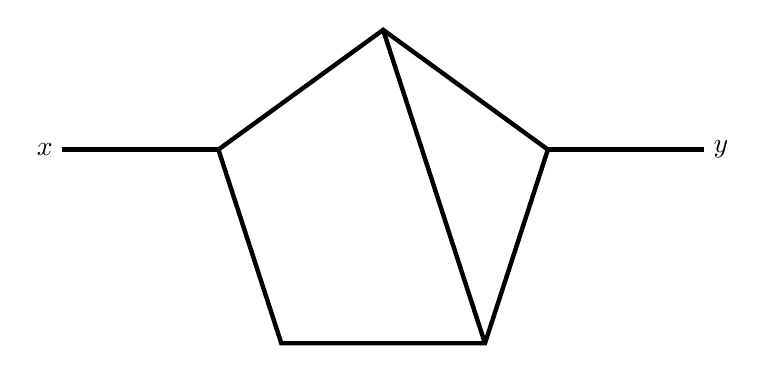
\begin{tikzpicture}[scale=2.2]%change the size here
	%pentagon
	\draw[ultra thick] (0,1)--(-0.9510565163,0.309017)--(-0.58778525229,-0.809017)--(0.58778525229,-0.809017)--(0.9510565163,0.309017)--cycle;
	%extra edges
	\draw[ultra thick] (0,1)--(0.58778525229,-0.809017);
	\draw[ultra thick] (-1.8510565163,0.309017)--(-0.9510565163,0.309017);
	\draw[ultra thick] (1.8510565163,0.309017)--(0.9510565163,0.309017);
	%label nodes   
	\node [left] at (-1.8510565163,0.309017) {$x$};
	\node [right] at (1.8510565163,0.309017) {$y$};
	\end{tikzpicture}
\end{center}

\begin{Exercise}[counter={sorszam}, difficulty=0]
	Azt mondjuk, hogy egy ir\'any\'itott %$G=(V,E)$
	gr\'af t\"om\"oren reprezent\'alt, ha adott egy $T$ Turing-g\'ep, ami $u,v$ bemenetre ki\'irja, hogy $uv$ \'el-e $\le n^k$ id\H oben, ahol $k$ egy fix konstans, pl.\ a feladat szempontj\'ab\'ol legyen $k=2$. A \la{Succinct-STconn} nyelv elemei azon $T$ Turing-g\'epek le\'ir\'asai, amik olyan gr\'afot t\"om\"or\'itenek, amiben van $st$ \'ut.\\
	a) Mutasd meg, hogy \PSPACE-ben eld\"onthet\H o \la{Succinct-STconn}.\\
	b) Mutasd meg, hogy \la{Succinct-STconn} \PSPACE-teljes.
\end{Exercise}	
\begin{Answer}
	a) \cl{NPSPACE}-beli \'es Savitch t\'etel.\\
	b) Az \'altal\'anos\'itott \'allapottere egy \PSPACE-es TG-nek pont egy ilyen gr\'afot ad.
\end{Answer}



\begin{Exercise}[counter={sorszam}, difficulty=2]
	a) A \la{Generalized Geography}-nak az a verzi\'oja is $\PSPACE$-teljes, ha a k\'et j\'at\'ekos k\"ul\"on-k\"ul\"on \'ep\'iti a saj\'at l\'anc\'at ugyanazon az ir\'any\'itott gr\'afon.
	(B\'armely cs\'ucsba csak egyik\"uk l\'ephet; mindkett\H onek meg van adva, hogy honnan kezd.)\\
	b) Ugyanez ir\'any\'itatlan gr\'afokra is $\PSPACE$-teljes.\\
	Mj.\ Azt nem tudom vizsg\'alt\'ak-e ezekben a verzi\'okban, hogy mi van, ha cs\'ucsokat szabad \'ujra haszn\'alni, csak az \'eleket nem.
\end{Exercise}	
\begin{Answer}
	Miltzow: Tron, a combinatorial Game on abstract Graphs \url{https://arxiv.org/abs/1110.3211} cikkben 13.~oldalt\'ol a), 15.\ oldalt\'ol b). (De egy\'ebk\'ent Nagy Kartal csin\'alt egyszer\H ubb megold\'ast r\'a.) 
\end{Answer}











\chapter{Véletlen algoritmusok}


\begin{Exercise}[counter={sorszam}, difficulty=-1]
	Adott egy $n$-edfokú polinom, és $n-1$ darab szám (nem feltétlen
	különbözőek). Ellenfelünk most azt állítja, hogy ennek a polinomnak
	multiplicitással éppen ezek a gyökei. Adjunk véletlent használó
	leleplező algoritmust, ami gyorsabb, mint a beszorzáson alapuló
	triviális determinisztikus eljárás.
\end{Exercise}


\begin{Exercise}[counter={sorszam}, difficulty=0]
	Adott egy \la{2-SAT} formula, amelyben minden klóz két különböző változót
	tartalmaz. \la{MAX2SAT}-nak nevezzük azt az optimalizálási feladatot, melynek célja
	a lehető legtöbb klózt igazzá tenni.
	\begin{enumerate}
		\item Adjunk gyors \emph{véletlen} algoritmust, amely nagy
		valószínűséggel olyan értékelést ad, amely a klózok legalább háromnegyedét
		igazzá teszi.
		\item Adjunk olyan determinisztikus polinomiális
		algoritmust, amely a klózok legalább háromnegyedét igazzá teszi.
	\end{enumerate}
\end{Exercise}

\begin{Exercise}[counter={sorszam}, difficulty=0]
	Hogyan tesztelhetj\"uk le gyorsan, hogy $q$ pr\'imhatv\'any-e?
\end{Exercise}	
\begin{Answer}
	Vegy\"uk $q$-nak az $i.$ gy\"ok\'et $i=1,\ldots,\log q$ \'ert\'ekekre \'es tesztelj\"uk mindr\H ol, hogy pr\'im-e.
	%max log q szamra kell tesztelni, hogy prim-e.
\end{Answer}

%\begin{Exercise}[counter={sorszam}, difficulty=-1]
%	Véges test felett vagyunk (bizonyos bonyodalmak elkerülése
%	végett). Adott három $n \times n$-es mátrix, $A,B,C$. Valaki azt állítja, hogy $AB=C$. Mi
%	ellenőrizni akarjuk ezt az állítást, úgy, hogy csak $O(n^2)$ szorzást végzünk,
%	de nem törekszünk teljes bizonyosságra: ha $AB \neq C$, akkor
%	$0.99$ valószínűséggel le akarjuk leplezni a csalást. Adjunk véletlen algoritmust
%	a feladatra.
%\end{Exercise}

\begin{Exercise}[counter={sorszam}, difficulty=0]
	Adj egy (RAM g\'epen) $\tilde O(n^2)$ idej\H u randomiz\'alt algoritmust, ami eld\"onti input $A,B,C$ $n\times n$-es eg\'esz m\'atrixokr\'ol, hogy $A\cdot B=C$ igaz-e. Melyik oszt\'alyban van ez az algoritmus \RP, \coRP \'es \BPP k\"oz\"ul?
\end{Exercise}	
\begin{Answer}
	$AB=C$ akkor \'es csak akkor, ha minden $x$-re $A(Bx)=Cx$, teh\'at ez val\'oj\'aban egy $n$ v\'altoz\'os line\'aris polinomazonoss\'ag tesztel\'es.
	Konkr\'etan egy v\'eletlen $x\in \{0,1\}^n$-re tesztelj\"uk, hogy $A(Bx)=Cx$ igaz-e.
	Ha $AB=C$, ez mindig teljes\"ul.
	K\"ulonben legyen $(AB)_{ij}\ne C_{ij}$.
	Ekkor csak egy $x_j$ \'ert\'ekre lesz $(A(Bx)_i=(Cx)_i$.
	Teh\'at legal\'abb $1/2$ es\'ellyel $A(Bx)\ne Cx$.
	Ez egy \coRP-beli algoritmus, teh\'at \BPP-beli is.
\end{Answer}

\begin{Exercise}[counter={sorszam}, difficulty=0]
	Az \Language nyelv eleme \RP-nek pontosan akkor, ha:
	
	Létezik egy olyan $p(n)$ polinom, és egy olyan \P-beli kétváltozós $M(x,y)$ reláció
	(olvasd: $y$ tanúja $x$-nek), hogy ha $x$ nem eleme \Language, akkor $x$-nek nincsen $p(|x|)$
	hosszú tanúja, ha $x$ eleme \Language, akkor viszont a $p(|x|)$ hosszú szavak legalább
	fele tanúja $x$-nek.
\end{Exercise}


\begin{Exercise}[counter={sorszam}, difficulty=0]
	Bizonyítsuk be, hogy az \RP definíciójában szereplő $1/2$-et tetszőleges
	$0<c<1$ konstansnak is választhattuk volna.
\end{Exercise}


\begin{Exercise}[counter={sorszam}, difficulty=0]
	Bizonyítsuk be, hogy a \BPP definíciójában szereplő $(1/3,2/3)$ helyett
	tetszőleges $(1/2-c,1/2+c)$ is állhatna, ahol $0<c<1/2$.
\end{Exercise}


\begin{Exercise}[counter={sorszam}, difficulty=-1]
	$\RP \subseteq \NP$, $\RP \subseteq \BPP$, $\cl{co-BPP} = \BPP$.
\end{Exercise}


\begin{Exercise}[counter={sorszam}, difficulty=0]
	Az \RP, \BPP, \ZPP nyelvosztályok mindegyike zárt a metszetre és unióra.
\end{Exercise}


\begin{Exercise}[counter={sorszam}, difficulty=0]
	\ZPP alábbi három definíciója ekvivalens:
	\begin{enumerate}
		\item Az algoritmus $1/2$-nél kisebb eséllyel passzolhat, és polinomiális futásidejű.
		\item Az algoritmus futásidejének várható értéke a bemenet hosszában polinomiális.
		\item $\RP \cap \cl{co-RP}$.
	\end{enumerate}
\end{Exercise}

\begin{Exercise}[counter={sorszam}, difficulty=0]
	$p(n)$ tetszőleges előre megadott polinom. \BPP definíciója ekvivalens mindkét alábbi
	definícióval: Létezik a nyelvhez olyan véletlen Turing-gép, amelynek tévedési valószínűsége
	\begin{enumerate}
		\item $2^{-p(n)}$ (erős \BPP definíció)
		\item $1/2-2^{-p(n)}$ (gyenge \BPP definíció)
	\end{enumerate}
\end{Exercise}


\begin{Exercise}[counter={sorszam}, difficulty=0]
	Mutasd meg p\'eld\'aul a \BPP -r\H ol, hogy ekvivalens defin\'ici\'okat kapunk, ha\\
	a) racion\'alis sz\'amok az eloszl\'asok (amik meghat\'arozz\'ak, hogy mikor merre l\'ep\"unk tov\'abb),\\
	b) csak egy darab \'allapot van, ami $1/2$--$1/2$ es\'ellyel l\'ep k\'et m\'asikba,\\
	c) van egy v\'eletlen szalagunk, melynek minden mez\H oje $1/2$ es\'ellyel 0 \'es 1,\\
	d) egy olyan p\'enzt ,,dob\'alhatunk'', ami valamilyen ismeretlen, konstans $p$ es\'ellyel lesz fej.\\
	e)~\hard Mutasd meg, hogyha az eloszl\'asr\'ol csak azt tessz\"uk fel, hogy rekurz\'iv,
	akkor $\BPP\not\subset \EXP$.
	\hint{ a) K\"ozel\'its\"uk a racion\'alis sz\'amokat diadikus racion\'alis sz\'amokkal az input hossz\'at\'ol f\"ugg\H o pontoss\'aggal. }
\end{Exercise}	
\begin{Answer}
	A b) az a) speci\'alis esete.\\
	Ha van egy a) t\'ipus\'u $T$ g\'ep\"unk, akkor abb\'ol \'ugy k\'esz\'ithet\"unk egy b) t\'ipus\'u $T'$-t, hogy ah\'anyszor randomiz\'alni kell, mindig le\'irjuk egy plusz szalagra, hogy \'eppen $T$ melyik \'allapot\'aban kell ezt megtenn\"unk, majd $T'$ egyetlen randomiz\'alt \'allapot\'aval addig sorsolunk, am\'ig el\'eg nagy pontoss\'aggal meg nem k\"ozel\'itj\"uk a racion\'alis sz\'amokat.
	A k\"ozel\'it\'es sz\"uks\'eges pontoss\'ag\'at, azaz azt, hogy a racion\'alis sz\'amot h\'any bin\'aris ``tizedes jegy'' pontoss\'agig sz\'amoljuk ki, az input hossza hat\'arozza meg.
	Ha $T$ $n^c$ id\H oben fut, akkor el\'eg $1/(2n^c)$ pontoss\'aggal k\"ozel\'iteni, \'igy az ebb\H ol ad\'od\'o hiba legfeljebb $(1-1/(2n^c))^{n^c}<1/e^2$, teh\'at az \"osszhiba legfeljebb $1/3+1/e^2<1/2$.
	Ez ism\'etl\'essel levihet\H o $1/3$ al\'a a szok\'asos m\'odon.\\
	A b) \'es c) ekvivalenci\'aja nyilv\'anval\'o.\\
	A d) speci\'alis esete a b)-c).\\
	Ha van egy b) t\'ipus\'u $T$ g\'ep\"unk, akkor abb\'ol \'ugy k\'esz\'ithet\"unk egy d) t\'ipus\'ut, hogy ah\'anyszor a randomiz\'al\'o \'allapotba l\'epn\'enk, dobjuk fel a p\'enzt k\'etszer.
	Ha fej-\'iras, l\'epj\"unk tov\'abb az egyik \'allapotba, ha \'iras-fej, akkor a m\'asikba, m\'ig ha k\'et azonos \'ert\'eket kapunk, akkor ism\'etelj\"uk ezt meg \'ujra.
	(Ha ezt olyan sokszor k\'ene megism\'etelni, hogy t\'ulmenn\'enk a megengedett fut\'asid\H on, akkor \'alljunk le, ennek \'ugyis kicsi az es\'elye.)\\
	e) Felismerhet\"unk egy olyan $L$ nyelvet, ami csak $x$ hossz\'at\'ol f\"ugg \'es annyira ritka, hogy csak $2^{2^t}$ alak\'u hossz\'us\'ag\'u szavak lehetnek $L$-ben.
	Azt, hogy $n$ benne van-e $L$-ben, ne lehessen \EXP-ben eld\"onteni, de $2^{2^n}$-ben m\'ar igen.
	Legyen egy \'allapot, amib\H ol $\sum_{n\in L} 1/n$ es\'ellyel l\'ep\"unk egy m\'asikba.
	\'Igy adott inputra kisebbekre meg tudjuk n\'ezni, hogy benne van-e, \'igy $n$ ism\'etl\'es ut\'an tudjuk, hogy kb.\ h\'any sikert v\'arunk, nagyobbak nem befoly\'asolj\'ak.
\end{Answer}

\begin{Exercise}[counter={sorszam}, difficulty=0]
	Eld\"onthetelen az \la{RP-ACCEPTANCE} nyelv, azaz, hogy egy le\'ir\'as\'aval adott randomiz\'alt, polinom id\H oben fut\'o Turing-g\'epr\H ol, hogy igaz-e, hogy
	minden $x$-et vagy legal\'abb $1/2$ es\'ellyel elfogad, vagy biztosan elutas\'it.
\end{Exercise}	
\begin{Answer}
	A meg\'all\'asi probl\'em\'at vezetj\"uk vissza.
	Input $T$-b\H ol k\'esz\'it\"unk egy $T'$-t, ami minden $x$ inputra $T$-t szimul\'alja a \"ures inputon $|x|$ l\'ep\'esig.
	Ha $T$ nem \'all le ezalatt, akkor $T'$ elutas\'it.
	Ha $T$ le\'all, akkor $T'$ fogadja el $|x|$-et $1/4$ es\'ellyel.
\end{Answer}


\begin{Exercise}[counter={sorszam}, difficulty=1]
	Egy adott konjunt\'iv norm\'alform\'ar\'ol valaki el\'arulja nek\"unk, hogy pontosan egy megold\'asa van (mint pl.\ egy Sudoku feladv\'anyn\'al). Mutassuk meg, hogy ha van polinomi\'alis algoritmus, ami megtal\'alja a megold\'ast, akkor $\RP=\NP$.	
\end{Exercise}	
\begin{Answer}
	Valiant-Vazirani t\'etel: \url{https://en.wikipedia.org/wiki/Valiant%E2%80%93Vazirani_theorem}.
	\end{Answer}

\begin{Exercise}[counter={sorszam}, difficulty=0]
	Ha \SAT eleme \BPP, akkor \SAT eleme \RP. (Ebből azonnal
	következik, hogy ha \NP része \BPP, akkor $\NP=\RP$. \wrk{Ennek prochat-nak kellene lennie, nem?})
\end{Exercise}


\begin{Exercise}[counter={sorszam}, difficulty=0]
	Érveljünk amellett, hogy $\DSPACE(O(n^{\log n}))$ nem része \BPP-nek. \wrk{Ezt a lecture05.ps-ben láttam, nem ismerem a megoldást.}
	
	\wrk{döm: szerintem ez nem nehéz, ha az alábbi megoldás jó.}
	
	\hint{Átlós módszer.}
\end{Exercise}

\sol{Felsoroljuk az összes véletlent használó Turing-gépet, mindet végtelen sokszor. Az $n$ hosszú inputokon az $n.$ Turing-gépet szimuláljuk addig, amíg $\le n^{\log n}$ tárat használ. Ha ezt bármikor túllépné, akkor leállunk. Mi nem tudunk véletlent használni, de sorban felírhatjuk az összes $n^{\log n}$ hosszú bitsorozatot, számoljuk, hogy melyikre mit outputolna a szimulált gép. (Ha több véletlen bitet használna, leállunk.) Végül pedig megnézzük, hogy mit outputolna többször és mi ennek az ellenkezőjét outputoljuk. Így biztos minden \BPP géptől eltértünk.}

\begin{Exercise}[counter={sorszam}, difficulty=0]
	\wrk{Yao tétele, kijelentve, hogy felhasználhatják Neumann minimax tételét.}
\end{Exercise}


\begin{Exercise}[counter={sorszam}, difficulty=0]
	Ha $\NP \neq \BPP$, akkor $\EXP \neq \cl{EXPSPACE}$.
\end{Exercise}




\begin{Exercise}[counter={sorszam}, difficulty=0]
	Legyen \PP azon nyelvek oszt\'alya, amikhez van minden inputra mindig polinomi\'alis id\H oben fut\'o randomiz\'alt Turing-g\'ep, ami $<1/2$ es\'ellyel hib\'azik.\\
	a) Mutasd meg, hogy $\NP \subseteq \cl{PP}$.\\
	b) $\cl{PP} \subseteq \PSPACE$.\\
	c) Mutasd meg, hogy ha a \PP -t v\'arhat\'o fut\'asid\H ovel defini\'aljuk, akkor
	az \'igy kapott oszt\'aly pontosan a rekurz\'iv nyelvek oszt\'alya lesz.
	\hint{ a) $\SAT\in\PP$, mert tippel\"unk egy tan\'ut, ha j\'o elfogadunk. Ha nem, akkor is elfogadunk $1/2-\eps$ es\'ellyel, valamint elutas\'itunk $1/2+\eps$ es\'ellyel. }
\end{Exercise}	
\begin{Answer}
	a) El\'eg azt bizony\'itani, hogy $\SAT\in\PP$.
	V\'alasszunk egy v\'eletlen \'ert\'ekad\'ast.
	Ha j\'o, akkor fogadjunk el.
	Ha nem j\'o, akkor is fogadjunk el $1/2-\eps$ es\'ellyel \'es utas\'itsunk el $1/2+\eps$ es\'ellyel.
	\'Igy ha $\Psi\notin \SAT$, akkor $>1/2$ es\'ellyel elutas\'itjuk, m\'ig ha $\Psi\in\SAT$, akkor legal\'abb $1/2^n+(1-1/2^n)(1/2-\eps)>1/2+1/2^{n+1}-\eps$ es\'ellyel elfogadjuk, teh\'at $\eps$-t v\'alaszthatjuk pl.\ $1/2^{n+2}$-nek.\\
	b) \PSPACE-ben v\'egig tudjuk sz\'amolni az \"osszes lehets\'eges fut\'asra az elfogad\'as val\'osz\'in\H us\'egek \"osszeg\'et.\\
	c) Ezek a Turing-g\'epek va\'oban csak rekuz\'iv nyelvet ismerhetnek fel, hiszen adott inputra addig sz\'amol\-gat\-hat\-juk, hogy mekkora es\'ellyel fogadnak/utas\'itanak el, am\'ig valamelyik $>1/2$ nem lesz.
	(Teh\'at a v\'arhat\'o fut\'asid\H ore nem is kell fels\H o korl\'at.)\\
	A rekurz\'iv nyelvek pedig val\'oban ebbe a csal\'adba tartoznak, hiszen el\'eg szimul\'alni egy, a nyelvet eld\"ont\H o Turing-g\'epet azzal a m\'odos\'it\'assal, hogy minden l\'ep\'es ut\'an $50\%$ es\'ellyel le\'allunk \'es v\'eletlenszer\H uen elfogadunk/elutas\'itunk.
	(Teh\'at a v\'arhat\'o fut\'asid\H o igaz\'ab\'ol lehet konstans is.)
	%http://cstheory.stackexchange.com/questions/8333/avarage-classes-for-pp-probabilistic-polynomial-time-and-ppt-machines-running/8425#8425
\end{Answer}


















\chapter{Polinomi\'alis hierarchia \'es or\'akulumok}

\section{Polinomi\'alis hierarchia}

\defi $\exists^p L := \left\{ x \in \{0,1\}^* \ \left| \ \left( \exists w \in \{0,1\}^{\leq p(|x|)} \right) \langle x,w \rangle \in L \right. \right\},$

\noindent
\'es hasonl\'oan $\forall^p L := \left\{ x \in \{0,1\}^* \ \left| \ \left( \forall w \in \{0,1\}^{\leq p(|x|)} \right) \langle x,w \rangle \in L \right. \right\}.$

\noindent
Ezekkel a jelölésekkel $\NP=\cl{\exists\cdot \P}$ és $\coNP=\cl{\forall\cdot \P}$. Ezen felbuzdulva $\Sigmak:=\cl{\exists\cdot\forall\cdot\exists\ldots \P}$ és $\Pik:=\cl{\forall\cdot\exists\cdot\forall\ldots \P}$, ahol összesen $k$ db kvantor áll a $\P$ el\H ott. Teh\'at ezekkel a jelölésekkel $\NP=\Sigmaone$ és $\coNP=\Pione$.
A polinomi\'alis hierarchia $\PH:=\cup \Sigmak$.
%Szint\'en elterjedt az $\MA=\cl{\exists\cdot \BPP}$ jel\"ol\'es.
%nem is uaz: https://complexityzoo.uwaterloo.ca/Complexity_Zoo:E#existsbpp

\begin{Exercise}[counter={sorszam}, difficulty=0]
	$\Sigmak\subset \Sigmakplus\cap\Pikplus$.
\end{Exercise}

\begin{Exercise}[counter={sorszam}, difficulty=0]
	$\Sigmak\subset\PSPACE$.
\end{Exercise}	

\begin{Exercise}[counter={sorszam}, difficulty=0]
	$\Pik\subset\Sigmak \Rightarrow \Sigmak=\PH$.
\end{Exercise}	

\begin{Exercise}[counter={sorszam}, difficulty=-1]
	Ha létezik \PH-teljes nyelv, akkor összeomlik a polinomiális hierarchia.
\end{Exercise}

\sol{ Tegyük fel, hogy létezik \PH-teljes nyelv, méghozzá a hierarchia $k$-dik szintjén lévő $L$ nyelv. Ekkor a hierarchia magasabb szintjein álló nyelvek visszavezethetőek rá, és \wrk{blabla kezdek teljesen elálmosodni}. }

\begin{Exercise}[counter={sorszam}, difficulty=0]
	Ha $\PH=\PSPACE$, akkor a hierarchiának csak véges sok szintje van.
	\hint{ El\H oz\H o miatt. }
\end{Exercise}


\begin{Exercise}[counter={sorszam}, difficulty=0]
	Tegy\"uk fel, hogy adva van egy konjukt\'iv norm\'al forma, melynek v\'altoz\'oi $x_i$-k \'es $y_i$-k. Azt szeretn\'enk eld\"onteni, hogy minden $x_i$ behelyettes\'it\'esre van-e az $y_i$-knek olyan behelyettes\'it\'ese, ami kiel\'eg\'it\H o. Mutassuk meg, hogy ez $\Pitwo$-ben van. Mi lenne, ha az lenne a k\'erd\'es, hogy van-e $x_i$, hogy minden $y_i$-re igaz a formula?
\end{Exercise}	 
\begin{Answer}
	Akkor trivin \Sigmatwo-ban lenne, de az is igaz, hogy \NP-beli, mert azt k\"onny\H u ellen\H orizni, hogy egy KNF-et minden \'ert\'ekad\'as igazz\'a tesz-e.
\end{Answer}

\begin{Exercise}[counter={sorszam}, difficulty=0]
	Legyen $L$ az $n^2\times n^2$ m\'eret\H u olyan \'altal\'anos\'itott Sudoku \'all\'asok nyelve, ahol ak\'arhova be\'irunk egy sz\'amot (nem azonos sorba/oszlopba/n\'egyzetbe egy ugyanolyan sz\'ammal), marad megold\'asa.\\
	a) Melyik oszt\'alyban van $L$?\\
	b) Nincs benne egy kisebben is?
\end{Exercise}	
\begin{Answer}
	\Pitwo-ban van trivi, de igaz\'ab\'ol \Sigmaone-ben is, mert az \"osszes lehet\H os\'eget leellen\H orizhetj\"uk.
\end{Answer}

\begin{Exercise}[counter={sorszam}, difficulty=1]
	$\NP \subset \Ppoly \Rightarrow \Sigmatwo=\PH$.
\end{Exercise}	
\begin{Answer}
	Karp-Lipton t\'etel.\\
	\"Otlet: El\H oször mutassuk meg, hogy ekkor olyan hálózat is van, ami minden kielégíthet\H o \SAT formulához ad egy helyes kiértékelést. Aztán mutassuk meg, hogy \"osszeomlana a polinomi\'alis hierarchia.
	
	Ha $\NP \subset \Ppoly$, akkor van egy $p(n)$ poly hossz\'u bitsorozat \'es $T$ TG, hogy $T(\Psi,p(n))=1$ akkor \'es csak akkor ha $\Psi\in\SAT$. S\H ot, olyan $T$ is van, hogy $T(\Psi,p(n))=1$ eset\'en m\'eg ki is ad egy $x$-et, amire $\Psi(x)$ igaz. Most azt fogjuk megmutatni, hogy $\Pitwo\subset\Sigmatwo$, ebb\H ol k\"ovetkezik az \'allit\'as. Legyen $L\in \Pitwo$. Ekkor $\Psi\in L$ akkor \'es csak akkor, ha minden $z$-re $\Psi_z\in \SAT$, valami \P-beli $\Psi_z$-re. De ez ekvivalens azzal, hogy $\exists p(n) \forall z T(\Psi_z,p(n))=1$ \'es $\Psi_z(x_z)$ igaz, ahol az $x_z$-t is $T$ adja ki.
\end{Answer}

\begin{Exercise}[counter={sorszam}, difficulty=1]
	$\EXP\subset \Ppoly \Rightarrow \EXP= \Sigmatwo$.
\end{Exercise}	
\begin{Answer}
	Meyer t\'etele (de Karp-Lipton cikkben van).\\
	El\H oz\H oh\"oz hasonl\'oan. Lenne egy hálózat, ami egy \EXP-es sz\'am\'it\'as b\'armelyik hely\'en, b\'armikor felvett \'ert\'eket meg tudn\'a mondani. Egy ilyennek a helyess\'eg\'et ellen\H orizni is tudjuk \coNP-ben.
	%forras: vargadanis
\end{Answer}

\begin{Exercise}[counter={sorszam}, difficulty=0]
	Tegyük fel, hogy adott egy játék, ahol két játékos felváltva lép és egy $poly(n)$ méret\H u táblán játszanak \'ugy, hogy felv\'altva elfoglalnak egy mez\H ot (pl.\ am\H oba). Az állás alapján mindig el lehet dönteni \P-ben, hogy nyert-e valaki. Tegy\"uk fel, hogy a játék $k$ lépés alatt garant\'altan véget ér. Mutassuk meg, hogy azon \'all\'asok nyelve, amikre kezd\H onek van nyer\H o stratégiája $\in \Sigmak$. S\H ot.
\end{Exercise}	
\begin{Answer}
	S\H ot (Borb\'enyi M\'arton), \P-beli, mert csak ennyi opci\'o van konstans k\"or\"os j\'at\'ekban \'es mindet v\'egign\'ezhetj\"uk.
	Ha a t\'abla exp m\'eret\H u lenne vagy k\"or\"onk\'ent $n$-et rakn\'anak, akkor csak \Sigmak-t tudn\'ank bizony\'itani.	
\end{Answer}

\begin{Exercise}[counter={sorszam}, difficulty=0]
	Igaz-e, hogy ,,G-ben pontosan $k$ méretű a legnagyobb klikk?'' eleme \Sigmatwo?
\end{Exercise}

\begin{Exercise}[counter={sorszam}, difficulty=1]
	Bizonyítsuk be, hogy \cl{\Sigma_4} nem része a $\SIZE(n^t)$ nemuniform bonyolultsági
	osztálynak, semmilyen fix $t$-re. \wrk{SIZE definiálandó? Ha igen, hol?}
	
	\hint{ Az alternációt használjuk fel arra, hogy tippeljünk egy nagy bonyolultságú Boole-függvényt, és ellenőrizzünk is le. }
\end{Exercise}

\begin{Exercise}[counter={sorszam}, difficulty=1]
	Az előző feladat és a Karp-Lipton tétel alkalmazásával lássuk be, hogy az
	előző feladat állítása \cl{\Sigma_4} helyett \Sigmatwo-vel is igaz.
	
	\hint{ Alkalmazzunk esetszétválasztást aszerint, hogy $\SAT \in \SIZE(n^t)$ \wrk{befejezetlen}. }
\end{Exercise}

\begin{Exercise}[counter={sorszam}, difficulty=0]
	A \la{MIN-DNF} nyelv párokból áll. A pár első tagja egy $\phi$ DNF formula. A második egy $k$ egész szám.
	A pár akkor van benne \la{MIN-DNF}-ben, ha létezik $k$-nál nem hosszabb $\psi$ formula, amely ekvivalens $\phi$-vel.
	Bizonyítsuk be, hogy \la{MIN-DNF} eleme \Sigmatwo.
\end{Exercise}

\section{Or\'akulumok}

\defi Az {\em orákulumos} Turing-gép egy többszalagos $M^?$ Turing-gép, melynek egyik szalagja a kitüntetett kérdez\H o-szalag. Az orákulum egy tetsz\H oleges $A$ nyelv lehet. $M^?$-nek van egy speciális $q_?$ állapota. Ha ebbe kerül, akkor az orákulum válaszol neki, hogy az éppen akkor a speciális szalagján lev\H o szó benne van-e az $A$ nyelvben. 

Az $x$ bemenethez tartozó kimenetet $M^A(x)$-szel jelöljük. Ha $\XP$ egy olyan nyelv, ami Turing-gépek egy speci\'alis családj\'aval van defini\'alva, akkor $\XP^A$ jelöli azokat az $L$ nyelveket, amihez van ebb\H ol a csal\'adb\'ol Turing-g\'ep, amihez $A$ orákulumot adva $L$-et ismeri fel. Ha valamely bonyolults\'agi oszt\'alyhoz van teljes nyelv, akkor gyakran a bonyolults\'agi oszt\'alyt \'irjuk a kitev\H obe, pl. $\P^{\NP}$ azt jelenti, hogy $\P^{\SAT}$. Ha nincs teljes nyelv, akkor is \'irhatunk bonyolults\'agi oszt\'alyt a kitev\H obe, ekkor az \'uj oszt\'aly az \"osszes lehets\'eges nyelv uni\'oja, pl.\ $\P^{\BPP}=\cup \{\P^{L}\mid {L\in \BPP}\}$.

\begin{Exercise}[counter={sorszam}, difficulty=0]
	Legyen $A$ egy $\P$-beli nyelv. Mutassuk meg, hogy $\P^A=\P$.
\end{Exercise}	
\begin{Answer}
	Futassuk magunk az $A$-t eld\"ont\H o TG-et ahelyett, hogy k\'erdezn\'enk t\H ole.
\end{Answer}


\begin{Exercise}[counter={sorszam}, difficulty=0]
	$\P^{\NP}=\P^{\SAT}$.
\end{Exercise}	
\begin{Answer}
	Minden \NP-beli nyelv visszavezethet\H o \SAT-ra, \'es azt\'an mint el\H oz\H o.
\end{Answer}


\begin{Exercise}[counter={sorszam}, difficulty=0]
	Ha $\E=\DTIME(2^{O(n)})$, akkor mi lesz $\P^{\E}$?
\end{Exercise}	
\begin{Answer}
	\EXP.
\end{Answer}

\begin{Exercise}[counter={sorszam}, difficulty=0]
	$\EXP^{\EXP} = \cl{EEXP}$. ($\cl{EEXP} = \DTIME(2^{2^{n^c}})$.)
\end{Exercise}


\begin{Exercise}[counter={sorszam}, difficulty=0]
	$\PSPACE^{\PSPACE}=\PSPACE$.
\end{Exercise}	
%\begin{Answer}
%\end{Answer}


\begin{Exercise}[counter={sorszam}, difficulty=0]
	Mutasd meg, hogy $\NP\cup \coNP\subset \P^{\NP}$.
\end{Exercise}	
\begin{Answer}
	$\NP\subset \P^{\NP}$ nyilv\'anval\'o \'es $\P^{\NP}$ z\'art komplementerre.
\end{Answer}


\begin{Exercise}[counter={sorszam}, difficulty=0]
	$\NP^{\NP\cap \coNP}= \NP$.
\end{Exercise}	
\begin{Answer}
	B\'armit k\'erdezn\'enk, megtippelhetj\"uk r\'a a v\'alaszt \'es tal\'alhatunk r\'a tan\'ut magunk.\\
	Forr\'as: \url{http://blog.computationalcomplexity.org/2017/03/np-in-zpp-implies-ph-in-zpp.html} alapj\'an.
\end{Answer}


\begin{Exercise}[counter={sorszam}, difficulty=0]
	$\NP^{\NP}= \Sigmatwo$.
\end{Exercise}	
\begin{Answer}
	$\NP^{\NP}\supset \Sigmatwo$ defin\'ici\'o szerint.
	$\NP^{\NP}\subset \Sigmatwo$-hez tippelj\"uk meg \"osszes k\'erd\'esre v\'alaszokat, amire van tan\'u, tippelj\"uk meg, amire nincs, azokra meg ez egyetlen $\Pione$-beli mondat, hogy egyikhez sincs.
\end{Answer}

\begin{Exercise}[counter={sorszam}, difficulty=1]
	$\BPP^{\BPP}=\BPP$.
	\hint{ Az or\'akulum nyelvhez van $\BPP$ algoritmus, ami $<1/2^n$ es\'ellyel hib\'azik. Ha ezt futtatjuk r\'a, akkor annak az es\'elye, hogy valaha is hib\'azunk k\'erdez\'es szimul\'al\'asakor kicsi. }
\end{Exercise}	
\begin{Answer}
	Legyen or\'akulumos TG fut\'asideje $n^k$ \'es hib\'azzon $<1/8$ es\'ellyel.
	Or\'akulum nyelvhez minden $n$-re \'es $k$-re van \BPP alg, ami $<1/(8n^k)$ es\'ellyel hib\'azik.
	Ez ism\'etelget\'essel kaphat\'o b\'armelyik \BPP-sb\H ol, teh\'at tudjuk is szimul\'alni $poly(n^k)$ id\H oben.
	Ha mindig ezt futtatjuk k\'erdez\'es helyett, akkor annak az es\'elye, hogy valaha is hib\'azunk k\'erdeze\'s szimul\'al\'asakor $<1/8$, teh\'at az \"osszhiba $<1/4$.
\end{Answer}

\begin{Exercise}[counter={sorszam}, difficulty=0]
	Igaz vajon, hogy $\RP^{\RP}=\RP$?	
\end{Exercise}	
\begin{Answer}
	$\coRP\subset \RP^{\RP}$, sz\'oval k\"ovetkezne bel\H ole $\coRP=\RP$, jelenleg nem ismert.
\end{Answer}

\begin{Exercise}[counter={sorszam}, difficulty=1]
	$\NP^{\BPP} \subseteq \BPP^{\NP}$.
\end{Exercise}

\begin{Exercise}[counter={sorszam}, difficulty=0]
	$\BPP \subseteq \ZPP^{\NP}$.
	
	\hint{ $\cl{pBPP}=\cl{pRP}^{\cl{pRP}}$. \wrk{opg5.ps} }
\end{Exercise}

\begin{Exercise}[counter={sorszam}, difficulty=0]
	Egy v\'eletlen $R$ nyelvre egy val\'osz\'in\H us\'eggel $\BPP\subsetneq \P^R$.	
\end{Exercise}	
\begin{Answer}
	Forr\'as: Charles H. Bennett, John Gill: Relative to a Random Oracle... \url{https://doi:10.1137/0210008}\\
	Ha $L\in \BPP$, akkor olyan Random TG is van, ami az \"osszes inputra \"osszesen $<1\%$-ot hib\'azik. Ezzel meg tudjuk mutatni, hogy a v\'eletlen nyelvek $99\%$-a tartalmazza $\BPP$-t, teh\'at egy val\'osz\'in\H us\'eggel $\BPP\subset \P^L$. Viszont egy val\'osz\'in\H us\'eggel $L \notin \BPP$, teh\'at egy val\'osz\'in\H us\'eggel $\BPP\ne \P^L$.
\end{Answer}

\begin{Exercise}[counter={sorszam}, difficulty=0]
	Mutass olyan $\XP$ bonyolults\'agi oszt\'alyt, amire $\XP^{\XP}\ne \XP$.
\end{Exercise}	
\begin{Answer}
	I. $\E$ vagy $\EXP$ j\'o id\H ohierarchia miatt.\\
	II. (Csern\'ak Tam\'as) Rekurz\'iv felsorolhat\'ok is j\'ok, mert nem z\'artak komplementerre.
\end{Answer}


\begin{Exercise}[counter={sorszam}, difficulty=0]
	$\exists A: \P^A= \NP^A$.
\end{Exercise}	
\begin{Answer}
	I. Ha $A$ \PSPACE-teljes, ez Savitch t\'etel.\\
	II. (\'Agoston P\'eter) $A=\PH$, mert ha nemdet $k$. szintr\H ol k\'erdez, det k\'erdezhet a $(k+1)$-edikr\H ol.
\end{Answer}


\begin{Exercise}[counter={sorszam}, difficulty=1]
	$\exists A: \P^A\ne \NP^A$.
\end{Exercise}	
\begin{Answer}
	Nyelv legyen, hogy van-e $A$-ban az inputtal megegyez\H o hossz\'us\'ag\'u string.
	Meg lehet csin\'alni \'atl\'os m\'odszerrel, hogy minden $\P$-belit\H ol k\"ul\"onb\"ozz\"on.
\end{Answer}


\begin{Exercise}[counter={sorszam}, difficulty=1]
	Van $A$ nyelv, hogy minden $L\in \NEXP^A$-hoz van $S\subset \N$ v\'egtelen halmaz \'es $L'\in\NP^A$, amire $L|_S=L'|_S$.
\end{Exercise}	
\begin{Answer}
	Forr\'as: Buhrman, Fortnow, Santhanam: Unconditional Lower Bounds Against Advice \url{https://doi.org/10.1007/978-3-642-02927-1_18}.
\end{Answer}














\chapter{H\'al\'ozatok}

\section{Általános Boole-hálózatok}

\begin{Exercise}[counter={sorszam}, difficulty=0]
	A méret polinomiális mértékű megnövelése árán elérhető, hogy az $AND,OR,NOT$ hálózat
	összes $NOT$ kapuja a legalsó szinten legyen.
\end{Exercise}


\begin{Exercise}[counter={sorszam}, difficulty=0]
	\begin{enumerate}
		\item Mely Boole-függvények számíthatóak ki Boole-hálózattal?
		\item Milyen $f(n)$-re igaz, hogy ekkora hálózat már minden $n$-változós Boole-függvényhez létezik?
	\end{enumerate}
\end{Exercise}


\begin{Exercise}[counter={sorszam}, difficulty=0]
	\begin{enumerate}
		\item Mely monoton Boole-függvények számíthatóak ki monoton Boole-hálózattal?
		\item Milyen $f(n)$-re igaz, hogy ekkora monoton hálózat már minden $n$-változós
		monoton Boole-függvényhez létezik?
	\end{enumerate}
\end{Exercise}


\begin{Exercise}[counter={sorszam}, difficulty=0]
	Adjunk $O(n \log n)$ méretű Boole-hálózatot a \la{MAJORITY} függvényre.
\end{Exercise}


\begin{Exercise}[counter={sorszam}, difficulty=1]
	Adjunk $O(n)$ méretű Boole-hálózatot a \la{MAJORITY} függvényre.
	
	\hint{ \wrk{Igaz-e az, hogy a bináris fát alkotó ismételt összeadással $\Sigma_i O(i)n/2^i = O(n)$ méretben vagyunk? Ha igen, akkor nem is nehéz.} }
\end{Exercise}


\begin{Exercise}[counter={sorszam}, difficulty=2]
	Ha \NP része \cl{P/log}, akkor $\P = \NP$.
	
	\hint{ Vegyük észre, hogy egy adott bemenetre egy adott \cl{P/log} algoritmust le tudunk futtatni minden egyes logaritmikus hosszúságú tanáccsal, polinomiális futásidőben maradva. De sajnos nincsen nyilvánvaló eljárás, amely eldönti, hogy a végigpróbálgatott tanácsok közül melyik a helyes. }
	
	\hint{ Azt kihasználva, hogy a \SAT eldöntési feladat $\cl{P/log}$-ban van, adjunk polinomidejű eljárást, amely megoldja a \SAT keresési feladatot. Az eljárásnak ne legyen bemenete a logaritmikus hosszúságú tanács, csak használja ki annak létezését. }
\end{Exercise}


\begin{Exercise}[counter={sorszam}, difficulty=2]
	Adjunk \PSPACE-beli nyelvet, amelynek az általános Boole-hálózat bonyolultsága
	$O( {n^3} / {\log n} )$ és $O(n^3)$ közé esik.
	
	\hint{ Először oldjuk meg a feladatot úgy, hogy elhagyjuk a \PSPACE-beliség feltételét, aztán adjunk \PSPACE-beli algoritmust a megtalált nyelvre. }
	
	\hint{ Az adott hálózati bonyolultságú nyelv megtalálásához először tekintsünk egy olyan nyelvet, amelynek a bonyolultsága $2^n/{3n}$ és $2^n$ közé esik. Ilyen nyelv Shannon tétele szerint létezik. Alkalmazzunk párnázást. \wrk{Tényleg ilyen jó konstanst ad Shannon tétele úgy, ahogy azt mi tanuljuk?} }
	
	\hint{ Ha egyáltalán létezik olyan nyelv, amelynek az általános Boole-hálózat bonyolultsága $c_2 {n^3} / {\log n}$ és $c_1 n^3$ közé esik, akkor ilyen nyelvet \PSPACE (konkrétan $\DSPACE(n^3)$) algoritmussal is tudunk találni: Sorban haladjunk végig a $c_1 n^3$ méretű hálózatokon. Álljunk meg, ha olyat találunk, amelynek egyetlen $c_2 {n^3} / {\log n}$ méretű hálózattal sem egyezik meg az igazságtáblája. A megtalált hálózatot értékeljük ki a bemenetünkön. }
	
	\hint{ Élesebb megoldás az első hintre: Jelöljük az $n^3-n-1$ méretű hálózatokkal kiszámítható $n$-változós Boole-függvények halmazát $F_n$-nel. Ez a halmaz nem üres, és nem esik egybe az összes $n$-változós Boole-függvények halmazával. Léteznek tehát olyan $f \in F_n$, $g \notin F_n$ $n$-változós Boole-függvények, amelyek csak egyetlen $a$ bemeneten különböznek. $g(x)=(x=a) \vee f(x)$ vagy $g(x)=(x=a) \vee f(x)$, tehát $g$ is kiszámítható legfeljebb $(n^3-n-1)+n+1=n^3$ méretű hálózattal. }
	
	\wrk{Mindezt midterm-sol.ps-ból loptam, jelölésestül, úgyhogy majd kreditet kell adni Luca Trevisan-nak. Az élesebb megoldást feladattá lehetne különíteni.}
\end{Exercise}


\begin{Exercise}[counter={sorszam}, difficulty=0]
	Bizonyítsuk be, hogy a monoton Boole-hálózatok kiértékelési feladata \P-teljes. \wrk{Melyik redukcióra?}
\end{Exercise}

\sol{ A nemtriviális irányhoz visszavezetjük a feladatra az általános Boole-hálózatok kiértékelési feladatát. A visszavezetés triviális, ha az általános Boole-hálózatainkat úgy definiáltuk, hogy csak a legalsó szintjén engedünk meg tagadó kapukat. Ekkor egyszerűen minden negált változóhoz felveszünk egy új változót, megkettőzve a változók számát, és monotonná téve a hálózatot. Ha az általános Boole-hálózatainknak magasabb szintjein is megengedünk tagadó kapukat, akkor ennek a triviális visszavezetésnek az alkalmazása előtt el kell végeznünk azt a polinom idejű átalakítást, amely a tagadó kapukat ,,lenyomja'' a hálózat legalsó szintjére. \wrk{Ez csak akkor elég részletes, ha ezt a lenyomást le tudom hivatkozni egy másik feladatba.}
}


\begin{Exercise}[counter={sorszam}, difficulty=0]
	Bizonyítsuk be, hogy a stratified Boole-hálózatok kiértékelési feladata \NL-teljes.
	Stratified-nak hívunk egy Boole-hálózatot, ha vagy csupa $AND$, vagy csupa $OR$ kaput tartalmaz.
\end{Exercise}


\begin{Exercise}[counter={sorszam}, difficulty=-1]
	Egy nyelv ritka, ha $n$ betűs szavainak száma $poly(n)$. A ritka nyelvek osztályát \SPARSE jelöli. \P-közelinek nevezünk egy \Language nyelvet, ha valamely $\Language' \in \P$ nyelvvel vett szimmetrikus differenciája ritka. \cl{P-close} a \P-közeli nyelvek osztálya. Bizonyítsuk be, hogy \cl{P-close} valódi része \Ppoly-nak.
	
	\hint{ Része, hiszen a szimmetrikus differencia belekódolható a tanácsba. A tartalmazás valódiságának bizonyításához tekintsük természetes számok egy nemrekurzív $H$ halmazát. Legyen $x \in \Language$ akkor és csakis akkor, ha $|x| \in H$. Ez az \Language nyelv \Ppoly, de nem \cl{P-close}. }
\end{Exercise}


\begin{Exercise}[counter={sorszam}, difficulty=1]
	Létezik olyan nyelv \PH-ban, amely nincs benne $\SIZE(O(n))$ -ben.
	
	\hint{ Ha \SAT egy ilyen nyelv, akkor készen vagyunk, tehát a megoldáshoz feltehetjük, hogy \SAT-ra létezik lineáris méretű hálózat-sorozat. }
\end{Exercise}


\begin{Exercise}[counter={sorszam}, difficulty=2]
	(Kannan tétele) Bizonyítsuk be a fenti állítást \PH helyett a $\Sigmatwo \cap \cl{\Pi_2}$ osztállyal.
\end{Exercise}

\sol{ \wrk{Nem tudom, hogy hol a megoldás, de Kannan-é az eredmény, és írnak róla itt: http://citeseer.ist.psu.edu/594507.html} }

\begin{Exercise}[counter={sorszam}, difficulty=-1]
	Ha $\NP \subseteq \SIZE(O(n))$, akkor $\P \neq \NP$. Használjuk fel Kannan tételét.
\end{Exercise}



%------------------------------

\section{Kis mélységű Boole-hálózatok}

\begin{Exercise}[counter={sorszam}, difficulty=0]
	\begin{enumerate}
		\item Adjunk alsó és felső becslést az $n$-változós \la{PARITY} függvényt kiszámító 2 mélységű Boole-hálózat méretére.
		\item Adjunk felső becslést az $n$-változós \la{PARITY} függvényt kiszámító 3 mélységű Boole-hálózat méretére.
	\end{enumerate}
\end{Exercise}


\begin{Exercise}[counter={sorszam}, difficulty=0]
	\begin{enumerate}
		\item Mutassunk lineáris méretű hálózatot, amelynek bemenete két
		$n$ bit hosszú szám, kimenete a két szám ($n+1$ bit hosszú) összege.
		(Minden kettes számrendszerben történik.)
		\item Az $x \geq y$ (más néven $\la{COMPARE}(x,y)$) reláció \ACnull-ban van.
		\item Az összeadás \ACnull-ban van.
		\item \hard Mekkora lehet egy \ACnull összeadó hálózat konstans mélysége?
	\end{enumerate}
\end{Exercise}


\begin{Exercise}[counter={sorszam}, difficulty=0]
	\wrk{Ugyanolyan nehéz az n darab n bites szám rendezése, mint az n darab egybitesé. Ugye ez igaz?}
\end{Exercise}


\begin{Exercise}[counter={sorszam}, difficulty=0]
	Tudjuk, hogy \la{PARITY} nem eleme \ACnull. Bizonyítsuk be, hogy
	\begin{enumerate}
		\item \la{MAJORITY} sem.
		\item \la{SORT} sem.
		\item $\la{MULTIPLY}(x,y)$ sem.
		\item $\la{DIVIDE}(x,y)=[x/y]$ sem.
	\end{enumerate}
\end{Exercise}


\begin{Exercise}[counter={sorszam}, difficulty=0]
	Most azt tudjuk, hogy \la{MULTIPLY} nem eleme \ACnull. Bizonyítsuk be, hogy \la{DIVIDE} sem.
\end{Exercise}


\begin{Exercise}[counter={sorszam}, difficulty=0]
	\la{PARITY} eleme \cl{TC^0}.
\end{Exercise}


\begin{Exercise}[counter={sorszam}, difficulty=2]
	\la{MAJORITY} eleme \cl{NC^1}.
\end{Exercise}

\sol{ \wrk{Az alábbiakban csak ész nélkül beegereztem Németh András megoldását. Megfésülendő, köszönetnyilvánítandó.}
	
	A MAJORITY kiszámítására a triviális technikát lenne jó alkalmazni:
	kiszámítjuk valahogy egy hálózattal a bitek első felén az egyesek
	számát, ill. ezzel párhuzamosan a bitek második felén, ezeket
	ábrázoljuk bináris számként, majd összaadjuk, és a kapott bináris
	számot összahasonlítjuk $n/2$-vel. A bitek első felén az egyesek
	számát természetesen rekurzívan akarjuk számítani: a bitek első
	negyedén levő egyesek száma és a bitek második negyedén levő egyesek
	száma összegeként. És így tovább, egyre kisebb számokat kell
	összeadnunk.
	
	Ez persze így bár helyes hálózatot eredményez, de mégsem oldja meg a
	feladatot, mert a hálózat túl mély lesz. Két $n$-bites szám
	összeadására ugyanis a triviális esetben cn mély hálózatot építenénk
	(általános iskolás összeadás hálósítása), így pl. $n=2^k$ esetén
	összesen $1+2+3+...+k=O(k^2)=O(\log^2(n))$ mély hálóra lenne
	szükségünk. Valójában létezik módszer k bites számok $O(\log k)$
	párhuzamos időben történő összeadására, de nekünk még ez sem lenne
	elég (ha jól sejtem ez $O(\log n\log\log n)$-et adna közvetlenül
	használva), de ennek a módszernek az egyik alapötletét fogjuk
	használni.
	
	Ábrázoljuk minden lépésben az adott szakaszokon található egyesek
	számát kiegyensúlyozott (pl.) négyes számrendszerbeli számként, azaz
	$\sum_{i=0}^k 4^ia_i$ alakban, ahol $a_i \in
	\{-3,-2,-1,0,1,2,3\}=:J$. Ez az ábrázolás persze nem egyértelmű, de
	sebaj. Két ilyen számot konstans mély hálózattal össze lehet adni.
	Könnyen elenőrizhető ugyanis, hogy ha $x,y \in J$, akkor $x+y$
	felírható $4a+b$ alakban, ahol $a \in {-1,0,1}$ és $b \in
	\{-2,-1,0,1,2\}$. Ez a felírás nyilván elvégezhető egy konstans
	méretű $E$ hálóval. Ha tehét két $n$ jegyű számot akarok összeadni,
	akkor egyszerre alkalmazom $E$-t az összes azonos helyiértékű
	számjegypárra, majd az $a$-ba kerülő helyiértéket hozzáadom a
	következő helyiértéken számított $b$-hez, ami a $b$-re és $a$-ra
	tett megkötés miatt már nem képez maradékot. Ezt az összeadást
	alkalmazva az első bekezdésben leírt módon egy $O(\log n)$ mélységű
	hálózattal ki tudom számítani az egyesek számát, amit egy
	kiegyensúlyozott, $O(\log n)$ jegyű négyes számrendszerbeli számként
	kapok meg. Ezt egy újabb $O(\log n)$ méretű hálózattal akár a
	triviális módon, a legkisebb helyiértéktől indulva standard alakra
	hozhatjuk. (Ehhez mindössze annyit kell észrevenni, hogy egy szám
	mod $4^k$ maradéka csak az utolsó $k$ számjegytől függ
	kiegyensúlyozott alakban is.) Még ugyanilyen mélységet igényel az
	összehasonlítás, így sikerült igazolni, hogy $MAJORITY \in NC^1$
	(Az, hogy az alkalmazott kapuk száma polinomiális $n$-ben, az
	triviális.)
	
	Megjegyzés: Egy $k$ jegyű kiegyensúlyozott szám valójában $O(\log k)$
	párhuzamos időben is standard alakra hozható, így áll össze az
	$O(\log k)$ párhuzamos idejű összeadás.
}


\begin{Exercise}[counter={sorszam}, difficulty=0]
	\la{SORT} eleme monoton \cl{AC^1}.
\end{Exercise}


\begin{Exercise}[counter={sorszam}, difficulty=1]
	A reguláris nyelvek \cl{NC^1}-ben vannak.
\end{Exercise}


\begin{Exercise}[counter={sorszam}, difficulty=0]
	$n$ darab $n$-bites szám összeadása \cl{TC^0}-ban van.
\end{Exercise}


\begin{Exercise}[counter={sorszam}, difficulty=0]
	$\la{MULTIPLY}(x,y)$ eleme $AC^1$. \wrk{Sőt, \cl{TC^0}-nak is eleme, ugye?}
\end{Exercise}


\begin{Exercise}[counter={sorszam}, difficulty=0]
	$n$ darab $n$-bites szám rendezése \cl{TC^0}-ban van.
	
	\hint{ Vegyük a páronkénti összehasonlításaikat. }
\end{Exercise}


\begin{Exercise}[counter={sorszam}, difficulty=0]
	Borogyin tétele: $\cl{NC^1} \subseteq \LOGSPACE$.
	
	\hint{ \wrk{(Du-Ko 6.24.) Először végezzünk el egy \LOGSPACE transzformációt, amely az adott bemeneti hálózatot formulává alakítja. Aztán értékeljük ki a formulát. Szétszedendő több feladatra.} }
\end{Exercise}


\begin{Exercise}[counter={sorszam}, difficulty=0]
	\begin{enumerate}
		\item Szimmetrikus Boole-függvény kiszámítható 3 mélységű, $2^{O(\sqrt{n} \log n)}$
		méretű hálózattal.
		\item \hard  Az állítás igaz $2^{O(\sqrt{n \log n})}$ méretkorlát mellett is.
		\item \veryhard Az állítás igaz $2^{O(\sqrt{n})}$ méretkorlát mellett is. \wrk{Én sem tudom.}
	\end{enumerate}
\end{Exercise}


\begin{Exercise}[counter={sorszam}, difficulty=0]
	Adott egy alul-felül $n$ csúcsú páros gráf, $n^2$ bittel leírva.
	\begin{enumerate}
		\item Adjunk $2^{O(n)}$ méretű konjunktív normálformát, ami megmondja, hogy van-e a gráfnak teljes párosítása.
		\item Bizonyítsuk be, hogy nem létezik a feladatra $2^{O(n)}$ méretű diszjunktív normálforma.
	\end{enumerate}
\end{Exercise}


\begin{Exercise}[counter={sorszam}, difficulty=0]
	Adaptálva Savitch tételének bizonyítását, bizonyítsuk be, hogy \NL része \cl{AC^1}.
\end{Exercise}


\begin{Exercise}[counter={sorszam}, difficulty=1]
	Elhanyagolva a nagyszámú és nehézkes uniformitási részletet, bizonyítsuk be Russo tételét:
	\begin{enumerate}
		\item \cl{NC^i} azonos a logaritmikus tárat felhasználó, $O(log^i n)$-time alternáló Turing-gépekkel felismerhető nyelvekkel.
		\item \cl{AC^i} azonos a logaritmikus tárat felhasználó, $O(log^i n)$-alternáló Turing-gépekkel felismerhető nyelvekkel.
		\wrk{Ez igazából nemigen adható fel, túl sok fura részlete van. Csak azért írtam ide, mert fontos.
			barrington - circuits - 23.pdf -ben van benne.}
	\end{enumerate}
\end{Exercise}

\defi Azon Boole-hálózatok a nem-unifom \cl{AC^i} hálózatok, amik polinomiális méret\H uek \'es $O(\log^i n)$ mélység\H uek.
Az uniform esetben kell egy $O(\log n)$ t\'ar\'u Turing-g\'ep is, ami el\H o tudja \'all\'itani a csal\'ad $n$. tagj\'at, ha a bemenete $n$).
Azok a \cl{NC^i} hálózatok, amik \cl{AC^i}-k és minden kapu befoka legfeljebb 2.
Az \"osszes uni\'oja a {\it Nick's Class}, jele (nem-uniform) \cl{NC}.
Ezek a j\'ol p\'arhuzamos\'ithat\'o algoritmusok.\\
Az el\H oad\'ason volt/lesz, hogy $\la{Parity}\notin\ACnull$.
Ha egy nem \ACnull-beli függvényt vissza tudunk vezetni valamire, akkor az sem lehet \ACnull-ban. Ennek felhasználásával (vagy n\'elk\"ul) mutassuk meg az alábbi függvényekr\H ol, hogy nincsenek \ACnull-ban, azaz az outputjuk valamelyik bitje nincs \ACnull-ban.

\begin{Exercise}[counter={sorszam}, difficulty=0]
	\cl{NC^0}$\subset$\cl{AC^0}$\subset$\cl{NC^1}$\subset\ldots$
\end{Exercise}	
\begin{Answer}
	A méret polinomiális megnövelése árán elérhet\H o, hogy minden kapu befoka kett\H o legyen.
	Hogyan v\'altozik a m\'elys\'eg? Legfeljebb a fok $\log$-szoros\'ara, ez legfeljebb a m\'eret $\log$-szorosa.
\end{Answer}

\begin{Exercise}[counter={sorszam}, difficulty=0]
	$\la{Compare}(x,y) \in \ACnull.$ ($\la{Compare}(x,y)=1$, ha $x\geq y$.)
\end{Exercise}

\begin{Exercise}[counter={sorszam}, difficulty=0]
	$\la{Sum}_i \in \ACnull.$
	($\la{Sum}_i(x,y)=x+y$-nak az $i$. jegye.)
\end{Exercise}
\begin{Answer}
	Akkor j\"on helyiértéktúlcsordulás (angolul carry) a $k$.\ helyre, ha van $m>m$, hogy $x_m=y_m=1$ \'es minden $k<j<m$-re $x_j+y_j\ge 1$. Ezt h\'al\'ozattal meg lehet csin\'alni.
\end{Answer}

\begin{Exercise}[counter={sorszam}, difficulty=0]
	$\la{Diff}_i \in \ACnull.$
	($\la{Diff}_i(x,y)=x-y$-nak az $i$. jegye, ha $x\ge y$, egy\'ebk\'ent 0.)
\end{Exercise}
\begin{Answer}
	Visszavezethetj\"uk az \"osszead\'asra \'ugy, hogy $x-y=x+(2^n-1-y)+1-2^n$.
\end{Answer}

\begin{Exercise}[counter={sorszam}, difficulty=0]
	$\la{Parity} \in \cl{NC^1}.$
	(A \la{Parity} outputja az inputok $mod$ 2 összege.)
\end{Exercise}

\begin{Exercise}[counter={sorszam}, difficulty=0]
	$\la{Majority} \in \cl{AC^1}.$
	($\la{Majority}(x)=1$, ha t\"obb 1-es van $x$-ben, mint 0-\'as.)
	%kijon az elozokbol, de SUM nem is fontos, mert ugyis csak log n hosszuakat adunk ossze.
\end{Exercise}

\begin{Exercise}[counter={sorszam}, difficulty=1]
	$\la{Majority} \in \cl{NC^1}.$
\end{Exercise}
\begin{Answer}
	K\"ovetkezik abb\'ol, hogy a $KW$-je minden szimmetrikus f\"uggv\'enynek $\log n$; l\'asd \ref{kwsym}.
\end{Answer}

\begin{Exercise}[counter={sorszam}, difficulty=0]
	$\la{Majority}\notin\ACnull$.
\end{Exercise}
\begin{Answer}
	\la{Majority}-b\H ol kij\"onne b\'armilyen Threshold gate ($\sum_i x_i\ge k$ t\'ipus\'u), ezekb\H ol p\'aratlanok ossze\'ESel\'es\'eb\H ol megvan \la{Parity}, ami viszont $\notin\ACnull$.
\end{Answer}

\begin{Exercise}[counter={sorszam}, difficulty=0]
	$\la{Multiply}(x,y)\notin\ACnull$.
\end{Exercise}
\begin{Answer}
	Ha sok null\'ast k\"ozberakva $x$-be, ezt megszorozzuk $10..010..01..$-val, k\"oz\'epen megjelenik \la{Parity} (meg kicsit arr\'ebb \la{Majority} is).
\end{Answer}

\begin{Exercise}[counter={sorszam}, difficulty=0]
	$\la{Square}\notin\ACnull$.
\end{Exercise}
\begin{Answer}
	$(x+y)^2-x^2-y^2$-ben ott lesz $xy$.
\end{Answer}

\begin{Exercise}[counter={sorszam}, difficulty=0]
	$\la{Cube}\notin\ACnull$.
\end{Exercise}
\begin{Answer}
	$(x+1)^3-x^3$-b\H ol megvan $3x^2$, amib\H ol $3xy$, amib\H ol 300030003-mal val\'o szorz\'as ugyan\'ugy neh\'ez, mint 1001..-val.\\
	V\'eg\'et befejezhetj\" uk \'ugy is (Schwartz Tam\'as, Borb\'enyi M\'arton), hogy $3x$-et szorozzuk az 1001../3-mal, amit bele tudunk dr\'otozni a h\'al\'ozatba.
\end{Answer}

\begin{Exercise}[counter={sorszam}, difficulty=0]
	Legyen $\la{Division-by-}c(x)=\lfloor \frac xc\rfloor$.
	Mit gondolsz, milyen $c$-kre lesz $\la{Division-by-}c\in\ACnull$?
\end{Exercise}
\begin{Answer}
	Kett\H ohatv\'anyokra trivi az. T\"obbi sz\'amra meg \la{Parity}-hez hasonl\'ot (pl.\ $\sum x_i \mod 3$-at) vissza lehet r\'a vezetni \"osszead\'asb\'ol (pl.\ $\sum x_i \mod 3=x-\lfloor \frac x3\rfloor-\lfloor \frac x3\rfloor-\lfloor \frac x3\rfloor$).
\end{Answer}

\begin{Exercise}[counter={sorszam}, difficulty=0]
	$\la{STconn} \in \ACone.$
\end{Exercise}
\begin{Answer}
	Savitch t\'etelhez hasonl\'oan felezget\"unk.
\end{Answer}

\begin{Exercise}[counter={sorszam}, difficulty=0]
	$\la{Perfect Matching} \stackrel ?\in \ACnull$, azaz el lehet-e d\"onteni konstans m\'elys\'egben, hogy van-e teljes p\'aros\'it\'as egy gr\'afban?
\end{Exercise}
\begin{Answer}
	Visszavezetj\"uk a \la{Parity}-t. Feleltess\"uk meg a v\'altoz\'okat egy gr\'af $n$ cs\'ucs\'anak, \'es legyen $x_ix_j$ \'el, ha $x_i=x_j$.
\end{Answer}

\begin{Exercise}[counter={sorszam}, difficulty=0]
	$\la{STconn} \stackrel ?\in \ACnull$, azaz el lehet-e d\"onteni konstans m\'elys\'egben, hogy van-e $st$ \'ut egy gr\'afban?
\end{Exercise}
\begin{Answer}
	(J.~Bird, l\'asd Furst--Saxe--Sipser: Parity, circuits, and the polynomial--time hierarchy) Visszavezetj\"uk a \la{Parity}-t. Tegy\"uk fel, hogy $x_1=x_n=1$ \'es feleltess\"uk meg a v\'altoz\'okat egy gr\'af $n$ cs\'ucs\'anak \'ugy, hogy $x_1=s$ \'es $x_n=t$.
	%Akkor legyen $x_ix_j$ \'el $i<j$-re, ha $x_i=x_j=1$ \'es pontosan egy $i<k<j$-ra lesz $x_k=1$.
\end{Answer}

\begin{Exercise}[counter={sorszam}, difficulty=0]
	$\la{Hamiltonicity} \stackrel ?\in \ACnull$, azaz el lehet-e d\"onteni konstans m\'elys\'egben, hogy van-e Hamilton--k\"or egy gr\'afban?
\end{Exercise}
\begin{Answer}
	I. Az el\H oz\H o feladat mint\'aj\'ara visszavezetj\"uk a \la{Parity}-t. Feleltess\"uk meg a v\'altoz\'okat egy gr\'af $n$ cs\'ucs\'anak, \'es legyen $x_ix_j$ \'el $i<j$-re, ha $x_i=x_j=1$ \'es minden $i<k<j$-re $x_k=0$ VAGY minden $k<i$-re \'es $k>j$-re $x_k=0$. Ez teh\'at vagy egy k\"or, vagy k\'et k\"or, parit\'ast\'ol f\"ugg\H oen. Az \"osszes $x_ix_j$ legyen \'el, ha $x_i=x_j=0$. Vegy\"unk fel m\'eg k\'et cs\'ucsot, akiket \"osszek\"ot\"unk mind az $n$ kor\'abbi cs\'uccsal. Mivel a 0-s r\'eszt csak \H ok k\"otik \"ossze az 1-es r\'esszel, ez\'ert pontosan akkor van Hamilton--k\"or, ha az 1-es r\'esz egy k\"orb\H ol \'all.\\
	II. (Borb\'enyi M\'arton) Visszavezetj\"uk, hogy annak eld\"ont\'ese, hogy egy $n$ hossz\'u 0--1 sorozatban ugyanannyi 1-es van-e, mint 0, az $\notin \ACnull$.
	(Ezt tudjuk, hiszen a \la{Majority}-hoz hasonl\'oan kij\"onne bel\H ole a \la{Parity}.)
	Feleltess\"uk meg a v\'altoz\'okat egy gr\'af $n$ cs\'ucs\'anak, \'es legyen $x_ix_j$ \'el, ha $x_i+x_j=1$.
\end{Answer}


\begin{Exercise}[counter={sorszam}, difficulty=0]
	Gondoljuk v\'egig, hogy \emph{uniform} h\'al\'ozatokra $\ACnull\varsubsetneq\NCone\subset\LOGSPACE\subset\NL\subset\ACone$.
\end{Exercise}
\begin{Answer}
	$\NCone\subset\LOGSPACE$, mert ki tudjuk \'ert\'ekelni a h\'al\'ozatot: csak $\log$ sok szint van.\\
	Az $\NL\subset\ACone$ meg $\la{STconn}\in \ACone$ miatt igaz.
\end{Answer}












\chapter{D\"ont\'esi f\'ak}

\begin{Exercise}[counter={sorszam}, difficulty=1]
	Tegy\"uk fel, hogy adott egy $n$ cs\'ucs\'u teljes p\'aros gr\'af. Egy l\'ep\'es megk\'erdezn\"unk, hogy k\'et adott cs\'ucsa k\"oz\"ott megy-e \'el. H\'any k\'erd\'esre van sz\"uks\'eg\"unk, hogy\\
	a) eld\"onts\"uk ugyanannyi cs\'ucs van-e mindk\'et oszt\'aly\'aban? ($n$ ps)\\
	b) tal\'aljunk egy cs\'ucsot, ami a nagyobb oszt\'alyb\'ol van? ($n$ pl)\\
	A v\'alasz mindk\'et esetben $n$-nek valami egyszer\H u f\"uggv\'enye.
\end{Exercise}	

\begin{Exercise}[counter={sorszam}, difficulty=0]
	Bizonyítsuk be, hogy a $\la{MAJORITY}(x_1,\dots,x_n) = \lfloor \sum_i{x_i} / 2 \rfloor$ zárkózott.
\end{Exercise}

\sol{ A zárkózottság bizonyításához ördög-módszert alkalmazunk: Ördögként bármelyik addig még nem kérdezett bitet kérdezik tőlünk, felváltva $1$-et és $0$-t válaszolunk. Kezdjük az $1$-gyel. Ez garantálja, hogy az utolsó kérdés előtt még nem megállapítható a függvény értéke. }

\begin{Exercise}[counter={sorszam}, difficulty=0]
	Mely $d$-kre zárkózott minden el\'eg nagy $n$-re, hogy egy $n$ jegy\H u input sz\'am $d$-vel oszhat\'o-e?
\end{Exercise}
\begin{Answer}
	Nem 2-hatv\'anyokra, mert b\'armely $d$-vel oszthat\'ora (pl.\ csupa null\'ara, ha azt is megengedj\"uk inputnak) a tan\'u $n$ hossz\'u.
\end{Answer}

\begin{Exercise}[counter={sorszam}, difficulty=0]
	Legyen $f_n=1$, ha egy $n$ hosszú bitsorozatban van két egymásutáni 1-es. Mennyi $D(f_n)$?
\end{Exercise}
\begin{Answer}
	$n$, kiv\'eve, ha $n\equiv 1 \mod 3$.
	Bizony\'it\'as megy indukci\'oval.
	Egy fontos megfigyel\'es, hogy ha valaki 1-es, akkor annak a szomsz\'edait is meg kell k\'erdezni el\H obb-ut\'obb, teh\'at feltehetj\"uk, hogy egyb\H ol meg lesznek k\'erdezve.\\
	Ehhez kapcsol\'od\'o cikk sok linkkel: \url{https://arxiv.org/abs/1712.09738}.\\
	Egy neh\'ez feladat cikkb\H ol: Van-e 101 r\'eszsorozat eld\"ont\'ese rejt\H ozk\"od\H o.
\end{Answer}

\begin{Exercise}[counter={sorszam}, difficulty=0]
	A {\la Cycle-free} gráftulajdonság zárkózott ha $n\ge 3$. 
\end{Exercise}
\begin{Answer}
	V\'alaszoljunk \'ugy, hogy fesz\'it\H of\'at kapjunk a v\'eg\'en.
	Egy megfelelő ördög-algoritmus a következő: Csak akkor válaszolunk nemmel egy él behúzottságát firtató kérdésre, ha az ,,igen'' válasz után már minden szóbajöhető gráfban lenne kör. (Azaz igyekszünk igennel válaszolni, de kerüljük, hogy kör jöjjön létre az igennel megválaszolt élekből.)
\end{Answer}

\begin{Exercise}[counter={sorszam}, difficulty=0]
	Az {\la STconn} gráftulajdonság zárkózott.
\end{Exercise}	
\begin{Answer}
	I. V\'alaszoljuk k\"ul\"onb\"oz\H o komponensbeliekre azt, hogy nem, kiv\'eve, ha ez a k\'et komponens k\"oz\"ott az utols\'o lehets\'eges \'el, akkor igen (hacsak nem az $s$ \'es a $t$ komponens\'er\H ol van sz\'o, akkor persze nemmel v\'alaszolunk az utols\'ora is).\\
	II. Az $st$-re azt mondjuk, hogy nem, az ezen k\'iv\"uli els\H o k\'erd\'esre meg, hogy igen. \'Igy k\'et cs\'ucsot \"osszeh\'uztunk \'es indukci\'ot haszn\'alhatunk. Ha a ,,dupla'' cs\'ucs egy \'el\'et k\'erdezn\'e az algoritmus, akkor el\H osz\"or mindig azt mondjuk, hogy nem, csak m\'asodj\'ara v\'alaszoljunk az indukci\'os algoritmus szerint.
\end{Answer}

\begin{Exercise}[counter={sorszam}, difficulty=0]
	Az ,,összefüggőség'' gráftulajdonság zárkózott.
	
	\hint{ Az ördög-algoritmus legyen a következő: Csak akkor válaszolunk igennel, ha a ,,nem'' válasz után már egyetlen gráf sem lenne összefüggő a szóbajöhetőek közül. (Azaz igyekszünk nemmel válaszolni, de vigyázunk arra, hogy a már behúzott és a még megkérdezetlen élek együtt összefüggő gráfot alkossanak. }
	
\end{Exercise}

\begin{Answer}
	\wrk{Nem hivatkozhatunk a hintre. Másoljuk be, ha már stabilizálódott.} Stratégiánk miatt a párbeszéd legvégén kapott gráf mindenképpen összefüggő lesz. Legyen $(u,v)$ az az él, amit utoljára, $\binom{n}{2}$-edikként \wrk{Használjuk azt, hogy nem lett vége hamarabb?} kérdezett meg a kérdező. Ördög-stratégiánk sikere azt jelenti, hogy a gráf összefüggősége függ attól, hogy ez az él be van húzva, vagy sem. Tegyük fel indirekt módon, hogy a gráf az utolsó $(u,v)$ él nélkül is összefüggő. Ekkor $u$ és $v$ között létezik $P$ út. Válasszuk ki ennek az útnak az utoljára megkérdezett $(w,z)$ élét. $(u,v)$ és az út többi éle olyan utat alkot $w$ és $z$ között, amely $(w,z)$ behúzásának pillanatában csupa behúzott vagy megkérdezetlen élből áll. Ebből könnyen következik, hogy $(w,z)$ behúzása nem befolyásolja a már behúzott és a még megkérdezetlen élek együttes gráfjának összefüggőségét. Ez azonban stratégiánk miatt ellentmondásban van azzal, hogy a $(w,z)$ él behúzottságára igennel válaszoltunk.
\end{Answer}

%ez szokott lenne eloadason
\begin{Exercise}[counter={sorszam}, difficulty=2]
	A ,,van izolált pontja'' gráftulajdonság zárkózott.
\end{Exercise}
\sol{ \wrk{A Gács-Lovász 58-59. oldalán. Nagyon nehéz. (Kati szerint nem nagy ötlet a második feladatot nagyon nehézre venni.) Az az ötlete, hogy páratlan sok gráf jöjjön szóba minden pillanatban, és mindig azt a választ adjuk, ami ezt a tulajdonságot megőrzi.} }

\begin{Exercise}[counter={sorszam}, difficulty=0]
	A ,,feszítőfa'' gráftulajdonság zárkózott.
\end{Exercise}


\begin{Exercise}[counter={sorszam}, difficulty=0]
	A ,,kétszeresen összefüggő'' gráftulajdonság zárkózott.
\end{Exercise}


\begin{Exercise}[counter={sorszam}, difficulty=0]
	A ,,legalább k-élű erdő'' gráftulajdonság zárkózott.
\end{Exercise}

\begin{Exercise}[counter={sorszam}, difficulty=0]
	a) Egy $n$ csúcsú gráf {\em skorpió}, ha van egy csúcsa (fej), ami össze van kötve $n-3$ darab csúccsal (lábak) és ezeken k\'iv\"ul m\'eg egy másodfokú csúccsal (farok), aminek a másik szomszédja egy els\H ofokú csúcs (fullánk). \wrk{Ábra.} (Teh\'at a l\'abak k\"oz\"ott lehetnek tov\'abbi \'elek.) Bizonyítsuk be, hogy egy gráfról $O(n)$ él lekérdezésével megállapítható, hogy skorpió-gráf-e.\\
	b) Hogyan kapcsol\'odik ez az Aanderaa-Karp-Rosenberg sejt\'eshez?
\end{Exercise}
\begin{Answer}
	%	\hint{ \wrk{http://www.cse.nd.edu/courses/cse511/www/solution1.pdf és http://www.cse.iitd.ernet.in/~sbaswana/Puzzles/Algo/algo.html\#Scorpio} }
	a) Vegy\"unk egy tetsz\H oleges $v$ cs\'ucsot \'es k\'erdezz\"uk v\'egig az \"osszes szomsz\'edj\'at. Ha $v$ foka 0 vagy $n-1$, akkor nem skorpi\'o a gr\'af. Ha $n-2$, akkor $v$ egyetlen nemszomsz\'edj\'at v\'egigk\'erdezve megtudjuk, hogy skorpi\'o-e. K\"ul\"onben $v$ se nem fej, se nem full\'ank.\\
	Ezut\'an vesz\"unk k\'et-k\'et cs\'ucsot a $v$-vel szomsz\'edosak \'es nemszomsz\'edosak k\"oz\"ul, \'es megk\'erdezz\"uk a k\"ozt\"uk lev\H o 6 \'elet. Ez alapj\'an valamelyikr\H ol kider\"ul, hogy szint\'en se nem fej, se nem full\'ank. Ezt csin\'ajuk, am\'ig szomsz\'edosakb\'ol vagy nemszomsz\'edosakb\'ol csak egy marad, majd arra is tesztelj\"uk, hogy nem fej vagy full\'ank-e.\\
	b) Mutatja, hogy kell a monotonit\'as.
	Ismeretlen forr\'asb\'ol: ``Originally Aanderaa and Rosenberg conjectured it without monotonicity, as $\Omega(n^2)$, Aanderaa showed this to be false with scorpion. Rivest and Vuillemin proved monotone with $\Omega(n^2)$, then Karp made sharp conjecture.''
\end{Answer}


\begin{Exercise}[counter={sorszam}, difficulty=0]
	Adott $n$ darab különböző szám. Feladatunk kiválasztani a legkisebbet és a
	legnagyobbat egyszerre. Hány összehasonlításra van ehhez szükség?
	
	\begin{enumerate}
		\item Megoldható $\left \lceil \frac{3n}{2} \right \rceil - 2$ összehasonlítással.
		\item \hard Ennyire szükség is van.
	\end{enumerate}
\end{Exercise}


\sol{ A felső becsléshez először osszuk párokba a számokat, és hasonlítsuk össze a párok két tagját. Ez $\lfloor n/2 \rfloor$ összehasonlítás. Ezek után már csak a ,,győztesek'' (nagyobbak) között keressük a legnagyobbat, és a ,,vesztesek'' között a legkisebbet. Mindkét részfeladat $\lceil n/2 \rceil-1$ összehasonlítást igényel.
	
	Az alsó becsléshez nevezzük nagyoknak azokat a számokat, amelyek az első összehasonlításuk alkalmával nagyobbnak lettek minősítve. A kicsik fogalmát analóg módon definiáljuk. Semmilyennek nevezzünk azokat a számokat, amelyek az algoritmus lefutásának adott pillanatában még egyszer sem lettek összehasonlítva másik számmal. Az alsó becsléshez a következő ördög-módszert alkalmazzuk: Ha egy nagyot és egy nem nagyot összehasonlítanunk, akkor jelöljük meg a nagyot nagyobbnak. Analóg módon járjunk el a kicsikkel is. Ha két semmilyet kell összehasonlítanunk, akkor természetesen tetszőlegesen dönthetünk. Ha két nagyot vagy két kicsit kell egymással összehasonlítanunk, akkor válaszoljunk tetszés szerint, de úgy, hogy ne kerüljünk ellentmondásba az addigi összehasonlításainkkal. (Más szóval az elvégzett összehasonlítások által meghatározott irányított gráfban ne jöjjön létre irányított kör. Ezt mindig megtehetjük, mert egy DAG-ba új élet behúzva az új él irányítható úgy, hogy a gráf DAG maradjon.)
	
	Az algoritmus futásának végére minden szám vagy nagy vagy kicsi lesz, hiszen a semmilyenekről nem tudhatnánk, hogy nem ők-e a legnagyobbak. A nagyok halmazán az összehasonlítások gráfja összefüggő, mert ha lenne két komponense, akkor akkor azok tetszőlegesen lennének rendezhetőek egymáshoz képest. Hasonló állítás igaz a kicsikre is. Ez legalább $n-2$ összehasonlítást jelent azonos kategóriájúak között. Ehhez jön a nagyok és kicsik között haladó összehasonlítások száma. Minden szám átesett legalább egy ilyenfajta összehasonlításon, hiszen a legelső összehasonlítása mindenképpen ilyen típusú volt. Tehát az ilyen összehasonlítások számára alsó becslés a két halmaz közül a nagyobbiknak a mérete, ami legalább $\lceil n/2 \rceil$.
}

\begin{Exercise}[counter={sorszam}, difficulty=0]
	Legfeljebb $2n-2- \lfloor \log n \rfloor$ kérdéssel eldönthető, hogy egy $n$ résztvevős tournamentben van-e olyan játékos, aki az összes többit legyőzte (abszolút győztes).
	
	\wrk{Zolinak nem tetszik a turnament szó? Vagy definiálni akarja?}
\end{Exercise}


\sol{ Először tartsunk egy $\lceil \log n \rceil$ fordulóból és $n-1$ mérkőzésből álló standard kieséses bajnokságot. Ennek az egyértelműen létező győztese az egyetlen szóbajöhető jelölt abszolút győztesnek. Játsszon mindenkivel, akivel a kieséses bajnokság során még nem játszott.}

\begin{Exercise}[counter={sorszam}, difficulty=2]
	Az előző feladatban adott korlát optimális.
	
	\hint{ Képzeljük el az algoritmus lefolyását úgy, hogy bajnokságot bonyolítunk le. Nevezzük valódinak azokat a mérkőzéseket, amelyek a mérkőzés megkezdéséig veretlenek között zajlottak. Vizsgáljuk a győztes által lejátszott valódi mérkőzések számát. }
	
	\hint{ Ördög-módszerünk legyen a következő: Egy veretlen és egy nem veretlen közötti mérkőzésen győzzön a veretlen. Két veretlen közti mérkőzésen győzzön az, akinek kevesebb valódi mérkőzése van. }
\end{Exercise}



\sol{ \wrk{Ide be kell egerezni a hinteket.} Az ördög-módszerünk alkalmazása során mindig marad legyőzetlen játékos, tehát a párbeszéd végén kapott turnamentben van abszolút győztes. $k$ szerinti teljes indukcióval bizonyítható, hogy mire egy játékos $k$ valódi játszmát megnyert, addigra ő és az általa addig kiejtettek összesen legalább $2^k-1$ valódi mérkőzést lejátszottak. A valódi mérkőzések összes száma $n-1$. Az abszolút győztes tehát legfeljebb $\lfloor \log n \rfloor$ valódi játszmát játszott. Mindenkit megvert, tehát pontosan $n-1$ (nem feltétlenül valódi) mérkőzést játszott. Ez az összes valódi mérkőzésekkel együtt már legalább $(n-1)+(n-1)-\lfloor \log n \rfloor$ játszma. }

\begin{Exercise}[counter={sorszam}, difficulty=0]
	Jel\"olje $K(x\mid y)$ a legr\"ovidebb program hossz\'at, ami kisz\'amitja $x$-et $y$-b\'ol. Mutasd meg, hogy $$\exists P\max_{x,y: f(x)\ne f(y)} \min_{i:x_i\ne y_i} 2^{\max\{K(i\mid x,P),K(i\mid y,P)\}} \le D(f).$$ %Laplante
\end{Exercise}


\begin{Exercise}[counter={sorszam}, difficulty=2]
	Egy 5 sz\'eles \emph{branching program} olyan, mint egy egyszer\H u d\"ont\'esi fa, de nem fa, csak egy szintezett ir\'any\'itott gr\'af, ami mindenhol legfeljebb 5 sz\'eles.
	Mutasd meg, hogy a polinom hossz\'u, 5 sz\'eles branching programokkal kisz\'am\'ithat\'o Boole f\"uggv\'enyek \'eppen a (nem-uniform) \NCone-beliek.
\end{Exercise}
\begin{Answer}
	Ez a Barrington-t\'etel.\\
	\"Otlet: Haszn\'aljuk fel, hogy $S_5$ nem feloldhat\'o!\\
	$\le$: Indukci\'oval trivi.\\
	$\le$: Feltehetj\"uk, hogy az \NCone h\'al\'ozatban csak \'ES \'es NEM kapuk vannak.
	Minden $d$ m\'ely ilyenhez csin\'alunk egy 5 sz\'eles h\'al\'ozatot, ami $4^d$ m\'ely.
	B\'armely szinten bel\"ul ugyanazt a v\'altoz\'ot k\'erdezz\"uk majd.
	5 lehets\'eges bemen\H o hely van, 5 kimen\H o hely, minden input ezeket permut\'alja.
	Azt mondjuk, hogy $P$ $\alpha$-kisz\'amolja $C$-t, ha $C(x)=0$-ra identit\'as, $C(x)=1$-re pedig $\alpha$ lesz a kimenet permut\'aci\'oja.\\
	Lemma 1: B\'armely k\'et 5-ciklus konjug\'alt, azaz minden $\alpha,\beta$-hoz van $\gamma$, hogy $\gamma^{-1}\alpha\gamma=\beta$.\\
	K\"ovetkezm\'eny: Ha $\alpha$-kisz\'amol\'os $P$ van, akkor $\beta$-kisz\'amol\'os $P'$ is (\'es legfeljebb 2-vel m\'elyebb).\\
	Lemma 2: Van $\alpha$ \'es $\beta$ 5-ciklus, hogy kommut\'aturuk is ciklus,
	azaz $\alpha\beta\alpha^{-1}\beta^{-1}=\gamma$.
	P\'eld\'aul: $\alpha= (1 2 3 4 5)$, $\beta = (1 3 5 4 2)$.
	Teh\'at b\'armilyen kaput tudunk szimul\'alni \'igy, k\'esz!
\end{Answer}

\bigskip
\defi Ha $f\not\equiv 1$ egy monoton n\"ov\H o Boole-f\"uggv\'eny, akkor legyen a hozz\'a tartoz\'o szimplici\'alis komplexus $K_f=\{S: f(S)=0\}$.

\begin{Exercise}[counter={sorszam}, difficulty=0]
	Ha $K_f$ nem kontrah\'alhat\'o, akkor $f$ zárkózott.
\end{Exercise}
\begin{Answer}
	(Pituk S\'ara) Tegy\"uk fel, hogy l\'etezik nem kontrah\'alhat\'o f\"uggv\'eny, ami nem z\'ark\'ozott \'es vegy\"uk ezek k\"oz\"ul azt az $f$ f\"uggv\'enyt, ami a lehet\H o legkevesebb helyen vesz fel 0-t, azaz $K_f$ minim\'alis.	
	$f$-re van $n-1$ m\'ely d\"ont\'esi fa, tekints\"unk egyet.
	Vegy\"uk egy $l$ level\'et, ahol $f=0$, \'es az ilyenek k\"oz\"ul a ,,legjobboldalibb'', azaz minden m\'as 0-lev\'elhez van egy olyan index, amin\'el $l$-ben 1 van, de a m\'asik lev\'elben 0.
	Az $l$ lev\'elhez k\'et input tartozik, att\'ol f\"ugg\H oen, hogy az utols\'o, nem ismert bit 0 vagy 1---el\H obbit jel\"olje $x_0$, ut\'obbit $x_1$.
	Ezeken k\'iv\"ul nincs olyan $y$ input, amire $y\ge x_0$ \'es $f(y)=0$, mert ez ellentmondana $l$ v\'alaszt\'as\'anak.
	Legyen $f'$ az a f\"ugv\'eny, ami pontosan $x_0$-ban \'es $x_1$-ben t\'er el $f$-t\H ol.
	Ha $K_f$ kontrah\'alhat\'o volt, akkor $K_{f'}$ is az lesz, hiszen $x_0$-ban ,,kipukkaszthatjuk''.
	De ez ellentmond $K_f$ minimalit\'as\'anak.\\
	Forr\'as: Kahn-Saks-Sturtevant t\'etel, l\'asd 19. oldal itt: \url{https://arxiv.org/abs/cs/0205031}.
\end{Answer}

\begin{Exercise}[counter={sorszam}, difficulty=1]
	Ha $f$ invari\'ans az inputj\'anak egy ciklikus permut\'aci\'oj\'ara, akkor z\'ark\'ozott. (Azaz $f(x_1\ldots x_n)=f(x_2\ldots x_nx_1)$ a felt\'etel.)
\end{Exercise}


\begin{Answer}
	\wrk{Nem hivatkozhatunk a hintre. Másoljuk be, ha már stabilizálódott.} Stratégiánk miatt a párbeszéd legvégén kapott gráf mindenképpen körmentes lesz. Legyen $(u,v)$ az az él, amit utoljára, $\binom{n}{2}$-edikként \wrk{Használjuk azt, hogy nem lett vége hamarabb?} kérdezett meg a kérdező. Ördög-stratégiánk sikere azt jelenti, hogy a gráf körmentessége függ attól, hogy ez az él be van húzva vagy sem. Tegyük fel indirekt módon, hogy a gráf az utolsó $(u,v)$ él behúzásával is körmentes. Ekkor $(u,v)$ elvágó él. Tekintsük az $(u,v)$ elhagyásával szétváló két komponens között haladó tetszőleges $(u,v)$-tól különböző $(w,z)$ csúcspárt. \wrk{, ami nem-él. Miért nem lehet a két komponens egy-egy elemű?} Könnyen látható, hogy $(w,z)$ megkérdezésének pillanatában a behúzása nem befolyásolja az igennel megválaszolt élek gráfjának körmentességét. Ez azonban stratégiánk miatt ellentmondásban van azzal, hogy a $(w,z)$ él behúzottságára nemmel válaszoltunk.
\end{Answer}













\chapter{Interakt\'iv}

\begin{Exercise}[counter={sorszam}, difficulty=0]
	Adj a one-time padhez hasonl\'o algoritmust, ami azt tudja, hogy A tud egy olyan \"uzenetet k\"uldeni, amit B \'es C egy\"utt meg tud fejteni, de egyed\"ul egyik\"uk sem.
\end{Exercise}
\begin{Answer}
	B-n\'el \'es C-n\'el is legyen egy titkos kulcs, amit a m\'asik nem ismer: $b,c\in\{0,1\}^n$. Ha A akar k\"uldeni egy titkos \"uzenetet, azt megteheti az $x\oplus b\oplus c$ k\'oddal. Tipikus rossz megold\'as volt, hogy $x\oplus r$ a k\'od \'es B ismeri a p\'aratlan, C meg a p\'aros bitjeit $r$-nek, de ez nem j\'o, mert \'igy b\'armelyik\"uk meg tudja fejteni $x$ fel\'et, mi pedig azt szeretn\'enk, hogy \emph{semmit} ne tudhassanak meg egyed\"ul $x$-r\H ol.
\end{Answer}

\section{Kommunik\'aci\'os bonyolults\'ag}

\defi A kommunik\'aci\'os j\'at\'ekban A \'es B játékos is ismeri az $f:\{0,1\}^n\times \{0,1\}^n\rightarrow \{0,1\}$ függvényt \'es mindkett\H oj\"uknek van egy inputja, $x$ illetve $y$, amit a másik nem lát. Az a feladat, hogy kisz\'amolj\'ak $f(x,y)$-t. Ehhez biteket küldhetnek egymásnak egy el?re megbeszélt protokoll alapján. Adott $f$-re a legjobb protokoll esetén a legrosszabb ($x,y$) párra k\"uldend\H o bitek sz\'am\'at jel\"olje $\kappa(f)$.
%eloadason ugy definialjak, hogy csak egyikuknek kell tudnia, masik meg tudja, hogy az egyik tudja.
%klikk vs independent set-re mar van log^2 n-es also: https://eccc.weizmann.ac.il/report/2015/050/

\begin{Exercise}[counter={sorszam}, difficulty=0]
	A $\ge$ feladatban $A$ \'es $B$ is kap egy sz\'amot $1$-t\H ol $2^n$-ig \'es el kell d\"onteni\"uk, hogy $A$ sz\'ama legal\'abb akkora-e, mint $B$-\'e. Mennyi $\kappa(\ge)$?
\end{Exercise}
\begin{Answer}
	I, A kommunik\'aci\'os m\'atrix rangja $2^n$, teh\'at a Mehlhorn-Schmidt t\'etel alapj\'an nincs jobb a trivi\'alis protokolln\'al.\\
	II, a kommunik\'aci\'os f\'aban az $(i,i)$ inputp\'arok mind egy-egy k\"ul\"onb\"oz\H o lev\'elbe kell, hogy ker\"uljenek.
\end{Answer}


\begin{Exercise}[counter={sorszam}, difficulty=0]
	A $MED$ feladatban $A$ \'es $B$ is $\{1\ldots,n\}$ egy-egy r\'eszhalmaz\'at kapja inputnak, az output pedig a k\'et halmaz uni\'oj\'anak medi\'anja (az uni\'ot multihalmaznak kell tekinteni, vagy tegy\"uk fel, hogy diszjunkt elemeket kapnak). Adj algoritmust, ami megoldja a feladatot\\
	a) $O(\log^2 n)$ l\'ep\'esben.\\
	b)~\hard $O(\log n)$ l\'ep\'esben.
	%ez kushilevitz-nisan konyvben 1.7-es feladat.
\end{Exercise}
\begin{Answer}
	a) A medi\'anjaik k\"oz\'e esik az uni\'o medi\'anja, ez\'ert el\'eg, ha minden l\'ep\'esben elk\"uldik egym\'asnak a medi\'anjaikat \'es az aktu\'alis halmazaik m\'eret\'et, majd akinek kisebb a halmaza, az az elemeinek a fel\'et ki tudja dobni (\'es m\'asik is ugyanennyit). \'Igy $\log n$ l\'ep\'es ut\'an egyik halmaz egyelem\H u lesz. Egy m\'asik megold\'as, hogy b\'armely sz\'amr\'ol $\log n+O(1)$ kommunik\'aci\'oval el tudjuk d\"onteni merre van t\H ole a medi\'an \'es \'igy bin\'arisan kereshet\"unk.\\
	b) \"Ugyesen keverj\"uk a fenti k\'et m\'odszert.
	%a)-hoz eleg a medianokat cserelni. vegyuk eszre, hogy ha regi medianok a<b voltak, akkor az igazi median a es b koze esik.
	%a) vagy az is jo k. keresesre, hogy megirjak n/2-nel hany nagyobb/kisebbjuk van.
	%a) padmini: barmely i szamrol log n-ben el tudjuk donteni, hogy merre van tole a median.
	%b)-hez csak (fontossagi sorrendben) bitenkent vetjuk ossze a medianokat. ha az uj medianok kozul vmelyik kiesik az intervallumbol, eleg O(1) bittel ezt lekommunikalni. ha mindketto beleesik, akkor kov fontossagi bitet nezzuk.
\end{Answer}

\begin{Exercise}[counter={sorszam}, difficulty=0]
	Defini\'aljuk a randomiz\'alt kommunik\'aci\'os bonyolults\'agot \'es adjunk gyors algoritmust az identit\'asra.
	%Itt ra kell jonni, hogy ket kulonbozo def van, mert rnd bitek lehetnek titkosak vagy nyilvanosak. 
\end{Exercise}
\begin{Answer}
	Egyik defin\'ic\'on\'al mindenki csak mag\'anak tud gener\'alni random biteket, m\'asikn\'al pedig k\"oz\"os random forr\'asuk van, pl.\ aznapi lott\'o sz\'amok.
	El\H obbi esetben $O(\log n)$ bittel megoldhat\'o, ha $x \mod p$-t elk\"uldik egym\'asnak egy random $p$ pr\'imre.\\
	\'Ut\'obbiban $O(1)$ bit is el\'eg ak\'ar a pr\'imes m\'odszerrel, ak\'ar $\langle x,r\rangle\stackrel ?\equiv \langle y,r\rangle \mod 2$-b\H ol.
\end{Answer}


\begin{Exercise}[counter={sorszam}, difficulty=2]
	Mutasd meg, hogy minden olyan $f$-re, aminek a m\'atrix\'anak b\'armely k\'et sora k\"ul\"onb\"ozik $R^{priv}(f)=\Omega(\log n)$, ahol $R^{priv}$ az el\H oz\H o feladatb\'ol a megfelel\H o defin\'ici\'o.
\end{Exercise}
\begin{Answer}
	L\'asd 19. oldal itt: \url{https://arxiv.org/abs/1007.1841}.%szakdogam
\end{Answer}


\begin{Exercise}[counter={sorszam}, difficulty=0]
	Egy fa k\'et r\'eszf\'aj\'anak diszjunkts\'aga eld\"onthet\H o\\
	a) $O(\log n)$ bittel.\\
	b)~\hard $\log n +\log\log n+O(1)$ bittel.\\
	c)~\veryhard Ez \'eles? (Nem tudom.)
\end{Exercise}
\begin{Answer}
	a) Egyik elk\"uldi b\'armelyik cs\'ucs\'at, m\'asik ehhez legk\"ozelebbij\'et.\\
	b) Fa cs\'ucsait sz\'amozzuk \'ugy, hogy els\H o $k$-t kit\"or\"olve minden komponens $<2n/k$. Ezut\'an elk\"uldj\"uk $k$ hossz\'at ($\log \log n$ bit), majd $k$-t, majd $\log(2n/k)$ m\'eret\H u v\'alaszt.
	Forr\'as: M. Saks and L. Lovasz,  "Lattices, mobius functions and communications complexity," FOCS 1988.\\
	c) \url{https://cstheory.stackexchange.com/questions/41524/what-is-the-exact-communication-complexity-of-subtree-disjointness}.
\end{Answer}

\chat{Ez a fejezet egyelőre lényegében csak Dömötör szövegének a beegerezése.
	
	\wrk{@0715 Elnevezzük a két játékost Alice és Bobnak? Egyelőre nem, de lehetne definiálni nevüket. Jelöléseket bevezetni? Ez szerintem hasznos lenne, beírtam párat.}
	
	Jelölések:\\
	$D(f)$: A legrosszabb esetben szükséges determinisztikus kommunikáció hossza.\\
	$N(f)$: A legrosszabb esetben szükséges nemdeterminisztikus kommunikáció hossza.\\
	$R(f)$: A legrosszabb esetben szükséges random kommunikáció hossza, ami az esetek$\leq \frac{1}{3}$ részében téved.\\
	$R^{pub}(f)$: A legrosszabb esetben szükséges random kommunikáció hossza, amikor a résztvevők közös random biteket kapnak és az esetek$\leq \frac{1}{3}$ részében téved.\\
}

\begin{Exercise}[counter={sorszam}, difficulty=0]
	Mindkét játékos megkapja egy-egy konvex $n$-szög csúcsainak koordinátáit. (Egy koordináta $O(\log n)$ hosszú.) Feladatuk eldönteni, hogy a két sokszögnek van-e közös belső pontja. $D(f)\leq O(\log^2 n )$.
	
	\hint{ \wrk{Yao-Ullmann-Yannakakis kell a legegyszerűbb megoldáshoz. De kijön anélkül is, $\log n$ lépésenként lehet felezni az egyik sokszög csúcsainak számát.} }
\end{Exercise}


\begin{Exercise}[counter={sorszam}, difficulty=0]
	Adott egy $G$ gráf. Egyik játékos kap egy klikket, a másik egy független csúcshalmazt. A kérdés, hogy van-e közös csúcsuk. $D(f)\leq O(\log^2 n )$.
\end{Exercise}


\begin{Exercise}[counter={sorszam}, difficulty=0]
	\begin{enumerate}
		\item Egyik játékos kap két $n$ hosszú 0-1 sorozatot, míg a másik ezek közül az egyiket. A cél, hogy a másik is tudja, melyiket. $D(f)\leq \log n+O(1)$.
		\item \hard Most ugyanaz a feladat, csak $k$ példányban, azaz az egyik játékosnak $k$-szor két inputja van, a másiknak pedig minden párból egy. $D(f)\leq \log n \log k\log \log k+O(k)$.
		\item Sőt, $D(f)\leq \log n \log k+O(k)$.
	\end{enumerate}
\end{Exercise}


\begin{Exercise}[counter={sorszam}, difficulty=0]
	\la{EQ} feladat: Mindkét játékos kap egy számot $1$-től $2^n$-ig. $R^{pub}(\la{EQ})=O(1)$.
\end{Exercise}


\begin{Exercise}[counter={sorszam}, difficulty=0]
	$R(\la{EQ})=O(\log n)$.
\end{Exercise}


\begin{Exercise}[counter={sorszam}, difficulty=2]
	Tudjuk, hogy az egyik játékosnak van $n$ db valóban különböző inputja, azaz bármely kettőhöz van a másiknak legalább egy olyan inputja, amivel más az output. $R(f)\geq\log n -o(\log n)$.
\end{Exercise}


\begin{Exercise}[counter={sorszam}, difficulty=2]
	\wrk{ezt szét akarom szedni több részre} Jelölje $D_{--}(f)$ annak a kommunikációs feladatnak az optimális megoldásának a hosszát, amikor a két játékos nem beszélhet egymással, hanem csak egy köztük ülő harmadikkal. A kommunikációt itt is az összes küldött bitben mérjük. $\exists f: D_{--}(f)\leq \frac{3}{2} D(f)+O(1)$.
\end{Exercise}




\section{Karchmer-Wigerson}

\defi Karchmer-Wigderson j\'at\'ek: Kommunik\'aci\'os j\'at\'ek egy verzi\'oja. A \'es B játékos is ismeri az $f:\{0,1\}^n\rightarrow \{0,1\}$ függvényt \'es mindkett\H oj\"uknek van egy inputja, $x$ illetve $y$, amit a másik nem lát. Azt is tudj\'ak, hogy $f(x)=0$ \'es $f(y)=1$. Az a feladat, hogy állapodjanak meg egy $i$ indexben, amire $x_i\neq y_i$. Ehhez biteket küldhetnek egymásnak egy el\H ore megbeszélt protokoll alapján. Adott $f$-re a legjobb protokoll esetén a legrosszabb esetben ($x,y$ párra) k\"uldend\H o bitek sz\'am\'at jel\"olje $KW(f)$.

\begin{Exercise}[counter={sorszam}, difficulty=0]
	Mutasd meg, hogy $KW(\la{Parity})=\Theta(\log n)$. (Azaz A inputjában páros, B inputjában páratlan sok $1$-es szerepel és kell találniuk egy eltérést.)
\end{Exercise}

\begin{Exercise}[counter={sorszam}, difficulty=1]
	Mutassuk meg, hogy ha csak az egyik\"uknek kell j\'ol tippelnie, akkor is kell $\log n+\Theta(1)$ bit. 
\end{Exercise}
\begin{Answer}
	Ha a kommunik\'aci\'o legfeljebb $\log n-3$ bit, akkor b\'armely fix inputra A csak az indexek kevesebb, mint negyed\'et tippelheti.
	Kett\H os lesz\'aml\'al\'asb\'ol az indexek t\"obbs\'ege olyan, hogy az inputok kevesebb, mint fel\'eben tippeli A.
	Ugyanez igaz B-re is, teh\'at lesz egy olyan index, amit egyik\"uk sem tippel az inputjaik t\"obbs\'eg\'eben.
	De ekkor lesz egy olyan inputp\'ar is, amik csak ebben a bitben t\'ernek el, \'es egyik\"uk sem tippeli soha ezt a bitet az adott inputra.
\end{Answer}	

\begin{Exercise}[counter={sorszam}, difficulty=1]
	Mutasd meg, hogy $KW(f)$ \'epp egyenl\H o a legsek\'elyebb $f$-et kisz\'am\'it\'o max.\ 2 befok\'u Boole-h\'al\'ozat m\'elys\'eg\'evel.
\end{Exercise}%erre le kene irni Kalina Kende meoldasat

\begin{Exercise}[counter={sorszam}, difficulty=1]\label{kwsym}
	Mutassuk meg, hogy ha $f(x)=g(|x|)$ (ahol $|x|=\sum_i x_i)$, akkor is el\'eg $O(\log n)$ bit ahhoz, hogy megállapodjanak egy $i$ indexben, amire $x_i\neq y_i$. 
\end{Exercise}
\begin{Answer}
	Ha m\'as a pari\'asuk, k\'esz. Ha parit\'as megegyezik, de 4-el osztva m\'as a marad\'ekuk, akkor is k\'esz. \'Igy el\H osz\"or megkeress\"uk a legkisebb kett\H o hatv\'anyt, amire k\"ul\"onb\"oznek, azt\'an ha m\'ar nem fognak, akkor lesz n\'ala kisebb is, amire fognak.
	
	Forr\'as: Brodal-Husfeldt: A Communication Complexity Proof that Symmetric Functions have Logarithmic Depth \url{https://www.brics.dk/RS/96/1/BRICS-RS-96-1.pdf}
\end{Answer}

\section{Zero-knowledge}

\begin{Exercise}[counter={sorszam}, difficulty=0]
	$\{(x,m): \exists y^2=x \mod m\}\in {\cl{PZK}}$, azaz adjunk egy gyors zero-knowledge protokollt, amivel bizony\'ithat\'o, hogy $x$ kvadratikus marad\'ek. (Nem kell a helyess\'eget teljes r\'eszletess\'eggel bizony\'itani!)
\end{Exercise}	
\begin{Answer}
	El\H osz\"or is feltessz\"uk, hogy $x$ \'es $m$ relat\'iv pr\'imek, vagy addig futtatjuk az euklideszi algoritmust, am\'ig azok nem lesznek.
	Azt\'an $P$ elk\"uldi $r^2$-et, majd $V$ v\'alaszt, hogy $r$-et akarja-e l\'atni vagy $ry$-t.
	Ha $x$ nem n\'egyzetsz\'am, akkor min $50\%$ az es\'elye, hogy $P$ bajban lesz.
	M\'asfel\H ol $V$ nem tud meg m\'ast, mint egy v\'eletlen sz\'amot \'es annak a gy\"ok\'et.\\	
	Ha szigor\'u defin\'ic\'o szerint akarjuk ez ut\'obbit megmutatni, akkor $P$-$V$ kommunik\'aci\'okat kell $V$-nek gener\'alnia. A szimul\'al\'ashoz vegy\"uk $r^2$-et \'es $r^2/x$-et $50$-$50\%$ es\'ellyel, mindkett\H o eloszl\'asa uniform.
	Ezut\'an ``sorsoljuk'', hogy $V$ azt fogja k\'erni, amit tudunk. 
\end{Answer}
%\hint{If $(x,m)=1$, Prover should first send a random quadratic residue $r^2$.} 



%\begin{Exercise}[counter={sorszam}, difficulty=0]
%\end{Exercise}	
%\begin{Answer}
%\end{Answer}
























\chapter{Kolmogorov-bonyolultság}

\defi Egy $U$ Turing-g\'ep univerz\'alis, ha minden $T$ Turing-g\'epre $U([T],x)=T(x)$, ahol a $[T]$ a $T$ le\'ir\'as\'at jelenti. Az $x$ Kolmogorov-bonyolultsága $U$ szerint a legr\"ovidebb program hossza, amire ki\'irja $x$-et, azaz $K_U(x)=\min \{|p|\mid U(p)=x\}$. Mostant\'ol azt is feltessz\"uk, hogy az \'ab\'ec\'e k\'etelem\H u. (Az els\H o sorban a vessz\H o az\'ert nem csal\'as, mert $[T]$-t \'irhatjuk kiterjesztett bin\'arisban.)


\begin{Exercise}[counter={sorszam}, difficulty=0]
	Minden $U,U'$-re van $C$, hogy $K_U(x)\le K_{U'}(x)+C$, sz\'oval az $U$-t ezent\'ul nem fogjuk ki\'irni.
\end{Exercise}	
%\begin{Answer}
%\end{Answer}

\begin{Exercise}[counter={sorszam}, difficulty=0]
	Mennyi az alábbi szavak Kolmogorov-bonyolultsága?\\
	a) $0101\ldots 01$. ($2n$ hosszú.)\\
	b) $11\ldots 1$. ($2^n$ db.)\\
	c) Az $n$.\ prímszám.
\end{Exercise}	
\begin{Answer}
	Ugyanannyi, ezt h\'ivhatjuk ak\'ar az $n$ sz\'am Kolmogorov-bonyolultság\'anak.
\end{Answer}

\begin{Exercise}[counter={sorszam}, difficulty=0]
	Igaz-e, hogy ha $x$ az $y$ els\H o n\'eh\'any jegye, akkor $K(x)\le K(y)$?
\end{Exercise}	
\begin{Answer}
	Nem, pl.\ ha $y=2^{2^n}$ darab 1-es, akkor annak lesz bonyolult prefixe.
\end{Answer}

\begin{Exercise}[counter={sorszam}, difficulty=0]
	Minden $n$ hosszú $x$-hez van $y$, ami legfeljebb egy helyen tér el t\H ole és $K(y)\leq n - \log n$.
\end{Exercise}	
\begin{Answer}
	\"Otlet: Hamming-k\'od legyen az $y$. De ebb\H ol csak akkor j\"onne ki sim\'an $n-\log n$, ha $n$ is meg lenne adva. Egy\'ebkent le lehet \'irni azt, hogy $y$ h\'anyadik Hamming-k\'odbeli elem az \"osszes (k\"ul\"onb\"oz\H o hossz\'us\'ag\'u) Hamming-k\'od k\"oz\"ul, ehhez $\sum_i 2^i/i$ kell. Ez indukci\'oval $O(2^n/n)$, pont j\'o.
\end{Answer}


\begin{Exercise}[counter={sorszam}, difficulty=0]
	Vegy\"unk egy j\'o nagy $N$ sz\'amot. Val\'osz\'in\H uleg a Kolmogorov-bonyolults\'aga is j\'o nagy lesz, azaz $K(N)\ge \log N - O(1)$. \'Es val\'osz\'in\H uleg van $N$-nek egy j\'o nagy pr\'imoszt\'oja, $p_k$, ami a $k.$ legkisebb pr\'im, azaz $k$ is j\'o nagy. Most \'ugy fogjuk elk\'odolni $N$-et, hogy le\'irjuk $k$-t \'es $N/p$-t (kettes sz\'amrendszerben). Ez persze $\log k$ illetve $\log (N/p_k)$ bit. Ezekb\H ol persze vissza tudjuk fejteni $N$-et, teh\'at $K(N)\le \log k + \log N - \log p_k +O(1)$, ahol az utols\'o tag a visszafejt\H o program le\'ir\'asa. Ezt \"osszevetve a kor\'abbi egyenl\H otlens\'eggel kapjuk, hogy $p_k=O(k)$, ami mintha ellentmondana a pr\'imsz\'amt\'etelnek, ha $k$ el\'eg nagy...
\end{Exercise}	
\begin{Answer}
	Ott a csal\'as, hogy nem mondtuk meg, hogy hol v\'egz\H odik a $k$ le\'ir\'asa. Ha rendesen sz\'amolunk, akkor abb\'ol kij\"on a pr\'imsz\'amt\'etel egy gyenge verzi\'oja.
\end{Answer}

\begin{Exercise}[counter={sorszam}, difficulty=0]
	a) Van olyan $c$, hogy semmilyen $x$-r\H ol nem bizony\'ithat\'o, hogy $c\le K(x)$. (Ha az axi\'omarendszer axi\'om\'ai rekurz\'ivan felsorolhat\'oak \'es $c$ f\"ugghet az \H oket felsorol\'o Turing-g\'ept\H ol meg a $K$ defin\'ici\'oj\'an\'al haszn\'alt $U$-t\'ol.)\\
	b)~\veryhard Van olyan TG, ami minden $x$ bemenetre kiír egy $L(x)\ne K(x)$ számot, amire $L(x)\le |x|$ \'es $\lim_{|x|\rightarrow\infty} L(x) \rightarrow\infty$? (Nyitott k\'erd\'es.)
	%elso 3 a 6.1.3-as mintajara megy, rutin kell legyen (legalabbis a-b)
	%b: nyitott \url{https://cstheory.stackexchange.com/questions/31282/can-we-not-output-the-Kolmogorov-complexity}
\end{Exercise}	
%\begin{Answer}
%\end{Answer}

\begin{Exercise}[counter={sorszam}, difficulty=1]
	Van-e olyan v\'egtelen $x$ sorozat, aminek b\'armely els\H o $n$ jegy\'ere igaz, hogy $K(x_1\ldots x_n)\ge n-\log n - C$ valamely $C$ konstansra?
\end{Exercise}	
\begin{Answer}
	Nincs, mert a sz\'o hossza is inform\'aci\'o, ezzel pont $\log n$-et lehet nyerni, ha szerencs\'enk van. Ezt m\'egegyszer elj\'atszva nyerhet\H o m\'eg $\log\log n$ stb.\\
	Forr\'as: Li-Vit\'anyi 2.5.1.
\end{Answer}

\begin{Exercise}[counter={sorszam}, difficulty=0]
	Bizony\'itsuk be Kolmogorov-bonyolults\'aggal, hogy egy v\'eletlen gr\'afban az \'atm\'er\H o nagy val\'osz\'in\H us\'eggel kett\H o.
\end{Exercise}	
\begin{Answer}
	K\'et t\'avoli cs\'ucs le\'ir\'asa $2\log n$, bel\H ol\"uk kimen\H o \'elek tov\'abbi $n \log_2 3$ a $2n$ helyett.
\end{Answer}

\begin{Exercise}[counter={sorszam}, difficulty=0]
	Bizony\'itsuk be Kolmogorov-bonyolults\'aggal, hogy van olyan tournament, amiben nincs $3 \log n$ m\'eret\H u tranzit\'iv r\'esztournament.
\end{Exercise}	
\begin{Answer}
	Tranzit\'iv r\'esz le\'ir\'asa sorrenddel $3\log n \cdot \log n$, m\'ig k\"ozt\"uk $\binom{3 \log n}2=4.5\log^2 n$ \'el megy.
\end{Answer}

\begin{Exercise}[counter={sorszam}, difficulty=1]
	Bizony\'itsuk be Kolmogorov-bonyolults\'aggal a Lov\'asz lok\'al lemma al\'abbi verzi\'oj\'at. L\'etezik $c>0$, hogy ha adva van n\'eh\'any $n$ m\'eret\H u kl\'oz \'ugy, hogy minden v\'altoz\'o legfeljebb $c2^n/n$ darab kl\'ozban szerepel, akkor minden kl\'oz egyszerre igazz\'a tehet\H o.
\end{Exercise}	
\begin{Answer}
	\"Otlet: Induljunk ki egy tetsz\H oleges \'ert\'ekad\'asb\'ol \'es am\'ig van, jav\'itsunk meg egy rossz kl\'ozt \'es az ez\'altal
	rossz\'a tett szomsz\'edokat. Egy jav\'it\'ol\'ep\'es, hogy egy kl\'oz $n$ v\'altoz\'oj\'anak \'uj \'ert\'eket adunk egy Kolmogorov-v\'eletlen $x$ sorozatb\'ol. Ha egy jav\'it\'assorozat t\'ul sok\'aig tartana, akkor $x$ nem lenne Kolmogorov-v\'eletlen.\\
	Forr\'as: Robin Moser \url{https://blog.computationalcomplexity.org/2009/06/Kolmogorov-complexity-proof-of-lov.html}
\end{Answer}


\begin{Exercise}[counter={sorszam}, difficulty=-1]
	$| K_{Java}(x) - K_{C++}(x) | \leq c_{Java,C++}$. \wrk{Kati szerint pongyola ez a jelölés.}
	
	\hint{ Java nyelven írhatunk C++ interpretert, és C++ nyelven Java interpretert. }
\end{Exercise}


\begin{Exercise}[counter={sorszam}, difficulty=-1]
	$P_{|x|=n}(K(x) \geq |x|-c) \geq 1-1/{2^c}$.
\end{Exercise}


\begin{Exercise}[counter={sorszam}, difficulty=-1]
	Létezik olyan $n$ szám, hogy az $n$-nél nagyobb prímek között nincsenek Kolmogorov-véletlenek.
	
	\hint{ Létezik olyan algoritmus, amely a $k$ bemenetre kiírja a $k$. prímszámot. }
\end{Exercise}

\sol{ A Prímszámtétel szerint egy tetszőleges $p$ prímszám legfeljebb a $\frac {9p} {8 \log p}$-edik a prímszámok sorában. Rögzítsünk egy olyan algoritmust, amely a $k$ bemenetre kiírja a $k$. prímszámot. (Például Erasztotenész szitáját implementálva.) A $k$ bemenetet a programba konstansként beledrótozva olyan algoritmust kapunk, amely $\log k+const$ méretű. Így egy legfeljebb $\log{\frac {9p} {8 \log p}}+const$ méretű algoritmust kaptunk tetszőleges rögzített $p$ prím kiírására. Elegendően nagy $p$ esetén ez a mennyiség kisebb lesz, mint $\log p-const$, amiből következik a bizonyítandó állítás. }


\begin{Exercise}[counter={sorszam}, difficulty=-1]
	Létezik olyan $n$ szám, hogy a $\pi$ $n$-nél hosszabb kettes számrendszerbeli
	közelítései között nincsenek Kolmogorov-véletlenek.
	
	\hint{ Létezik olyan algoritmus, amely a $k$ bemenetre kiírja $\pi$ első $k$ számjegyét. }
\end{Exercise}

\sol{ Tekintsünk valamilyen $\pi$-hez konvergáló racionális végtelen sorozatot, amelynek becsülni tudjuk a konvergenciasebességét. (Ez lehet például a Leibniz-formula, lehet a $2 \arctan(1)$ Taylor-sora, vagy a modern, úgynevezett Borwein iteráció.) Látható, hogy ez alapján építhetünk egy algoritmust, amely $\pi$ egyre pontosabb racionális közelítéseit számolja, hibabecsléssel együtt. Ezt felhasználva könnyen építhetünk olyan algoritmust, amely a $k$ bemenetre kiírja $\pi$ első $k$ számjegyét. A $k$ bemenetet a programba konstansként beledrótozva olyan algoritmust kapunk, amely $\log k+const$ hosszú, és kiírja $\pi$ első $k$ számjegyét. Elegendően nagy $k$-ra ez kisebb lesz, mint $k-const$, tehát nagy $k$ értékekre a kimenetek nem lehetnek Kolmogorov-véletlenek. }


\begin{Exercise}[counter={sorszam}, difficulty=0]
	Nem létezik olyan algoritmus, amely minden $x$-hez megmondja $K(x)$-et.
\end{Exercise}

\sol{ Indirekt feltételezve $K(x)$-et meghatározó algoritmus létezését, azt szubrutinként
	használhatjuk olyan program írására, amely kiírja a lexikografikusan első olyan $x$ szót,
	amelynek bonyolultsága egy adott $k$ számnál nagyobb. Programunk bonyolultsága
	$const+\log k$-val becsülhető felülről, ahol a $\log k$
	mennyiség a $k$ szám programba való ,,beégetéséből'' származik. Kellően
	nagy $k$ számot választva ellentmondásra jutunk. }


\begin{Exercise}[counter={sorszam}, difficulty=0]
	Nem létezik olyan algoritmus, amely a $K(x)$ olyan $L(x)$ közelítését számítja ki,
	amelyre minden $x$ szóra $0.9 K(x) \leq L(x) \leq 1.1 K(x)$.
\end{Exercise}


\sol{ A megoldás lényegét tekintve azonos az előző feladat megoldásával, hiszen
	az $L(x)$ közelítést kiszámító szubrutin is
	alkalmazható arra, hogy megkeressünk egy olyan $x$ szót,
	amelynek bonyolultsága biztosan nagyobb egy adott $k$ számnál.
	\wrk {Akkor itt most megsértettem azt az elvet, hogy nem hivatkoznak egymásra, de itt talán tényleg indokolt volt.} }


\begin{Exercise}[counter={sorszam}, difficulty=0]
	Bizonyítsuk be, hogy minden $n$ hosszú $x$ szóhoz létezik olyan $y$ szó, amely
	$x$-ből csupán egyetlen bit megváltoztatásával áll elő, ugyanakkor $K(y|n) \leq n - \Omega (\log n)$.
	\wrk{A $K(y|n)$ jelölést be kell vezetni.}
	
	\hint{ Használjunk Hamming-kódolást. }
\end{Exercise}

\sol{ A Hamming-kódok elméletéből tudjuk, hogy az $n$-dimenziós kocka csúcsainak létezik egy olyan $H$ részhalmaza, amelyre igaz, hogy 1. A kocka minden csúcsától legfeljebb egy távolságra található $H$-beli elem, 2. $H$ mérete legfeljebb \wrk{$2^{n-\lfloor \log (n+1) \rfloor }$ }. $H$ egy tetszőleges eleme $n$ ismeretében specifikálható azzal, hogy a lexikografikus rendezés szerint hányadik elemről van szó $H$-ban. A feltételeket kielégítő $y \in H$ tehát $\lceil \log |H| \rceil = n - \Omega(\log n)$ bit információval írható le. }


\begin{Exercise}[counter={sorszam}, difficulty=0]
	Létezik olyan $c$, hogy minden Kolmogorov-véletlen $x$ szóra az egyesek
	számának és a nullák számának különbsége legfeljebb $c \sqrt{|x|}$.
	
	\hint{ Ha $k$ az egyesek száma a szóban, akkor kódolhatunk úgy, hogy
		megadjuk $|x|$-et, $k$-t, és azt, hogy az $\binom{|x|}{k}$ lehetőség
		közül melyik valósul meg. Alkalmas $k$-ra ez a kódolás tömörítés lesz. }
\end{Exercise}

\sol{ Ha $k$ az egyesek száma a szóban, akkor kódolhatunk úgy, hogy
	megadjuk $|x|$-et, $k$-t, és azt, hogy az $\binom{|x|}{k}$ lehetőség
	közül melyik valósul meg. Ennek a kódolásnak a hossza $O(\log |x|) + O(\log k) + O(\binom{|x|}{k}) \leq $ Alkalmas $k$-ra ez a kódolás tömörítés lesz. \wrk{Számoljuk ki.} }


\definition{ Elegánsnak hívunk egy programot, ha ő a legrövidebb azok közül, akik
	az ő kimenetét adják. (Esetleg holtversenyben.) }

\begin{Exercise}[counter={sorszam}, difficulty=-1]
	Minden elegáns program Kolmogorov-véletlen.
\end{Exercise}

\sol{ Ha konstansnál több bitet tömöríthetünk egy programon, akkor a tömörített változatát kitömörítő majd lefuttató
	program rövidebb nála, miközben azonos kimenetet ad. }


\begin{Exercise}[counter={sorszam}, difficulty=0]
	Minden axiómarendszerhez csak véges számú olyan $p$ program létezik, amelynek
	eleganciája bizonyítható a rendszerben. (Mindeközben végtelen sok elegáns program létezik,
	tehát léteznek bizonyíthatatlan igaz állítások az axiómarendszerben.)
\end{Exercise}

\sol{ Tekintsünk egy olyan programot, amely az axiómarendszer összes lehetséges bizonyítását
	enumerálva bizonyítható állításokat bocsát ki. A program kimenetét vezessük át egy
	olyan szűrőprogramon, amely (tisztán formális ismérvek alapján) csak olyan állításokat enged
	át, amelyek valamely program eleganciáját jelentik ki. Legyen $k$ később meghatározandó
	nagy természetes szám. Ha a szűrő végtelen sok állítást enged át magán,
	akkor előbb-utóbb kibocsát olyan állítást, amely egy $k$-nál hosszabb
	program eleganciáját jelenti ki. Az első ilyen állítás megtalálásakor futtassuk le a
	megtalált hosszú és elegáns programot, majd állítsuk le összes program-modulunkat. Mi a kiírt szó
	Kolmogorov-bonyolultsága? A szűrőn átengedett állítás szerint legalább $k$. Másrészt
	programunk minden összetevője (bizonyítás-enumeráló, szűrő, szimulátor)
	az axiómarendszer rögzítése mellett konstans hosszúságú,
	tehát a programunk bonyolultsága $const+\log k$-val becsülhető felülről, ahol a $\log k$
	mennyiség a $k$ szám programba való 'beégetéséből' származik. Kellően
	nagy $k$ számot választva ellentmondásra jutunk, amelynek egyetlen lehetséges feloldása,
	hogy a szűrőprogram csak véges sok állítást enged át magán. }









\chapter{Tartalékok}

\begin{Exercise}[counter={sorszam}, difficulty=0]
	Egy $n$ szám $m$ modulus szerint vett $t$-edik hatványát ki tudjuk számolni polinomidőben.
	(Mindhárom bemenet kettes számrendszerben van megadva.)
\end{Exercise}

\sol{ Egy $n$ szám $m$ modulus szerint vett négyzetét természetesen ki tudjuk számolni polinomidőben. A négyzetre emelés műveletét ismételgetve a negyedik, nyolcadik, stb. hatványát is ki tudjuk számolni polinomidőben, amíg a négyzetre emelések összes száma polinomiális. $t$ kettes számrendszerbeli felírása legyen $2^{i_1}+\dots+2^{i_k}$. Ez alapján $n^t = n^{2^{i_1}+\dots+2^{i_k}} = \prod_l{n^{2^{i_l}}}$. Ennek a szorzatnak minden tényezője kiszámolható polinomidőben, és összesen polinomiális számúan vannak. }


\begin{Exercise}[counter={sorszam}, difficulty=-1]
	Egy $n$ szám $t$-edik hatványát nem tudjuk kiszámolni polinomidőben az egészek között.
\end{Exercise}


\begin{Exercise}[counter={sorszam}, difficulty=0]
	Egy $[n]$ feletti $p$ permutáció $t$-edik hatványát ki tudjuk számolni
	polinomidőben. ($t$ kettes számrendszerben van megadva.)
\end{Exercise}

\sol{ \wrk{Annyira azonos a megoldás az előzővel, hogy restellem is leírni. $n$ helyett $p$-t kell írni.} }


\begin{Exercise}[counter={sorszam}, difficulty=0]
	http://www.cl.cam.ac.uk/Teaching/2003/Complexity/exercise1.pdf \la{HORN-SAT} \P-beli, és \P-teljes a \LOGSPACE-redukcióra nézve. Utóbbihoz kell a konkrét visszavezetés nemdeterminisztikus eldöntésről \SAT-ra. Ez ügyesen csinálható úgy determinisztikus gépekre, hogy Horn-formulát adjon.
\end{Exercise}


\begin{Exercise}[counter={sorszam}, difficulty=1]
	\wrk{Dömötöré. Mik ezek a példák? A szimmetrikus az, hogy $xx$ alakú? Akkor hamis az állítás. Nem értem.} A nem szimmetrikus szavak (pl $baba$ szimmetrikus, de $bababa$ vagy $babab$ nem) nyelve környezetfüggetlen.
	\wrk{döm: De igaz...}
	\hint{$uauvbv$ nem szimmetrikus}
\end{Exercise}

\sol{A páros hosszú szavak előállításához az alábbi műveletek kellenek: $S\rightarrow AB, S\rightarrow BA, A\rightarrow xAy, B\rightarrow xBy, A\rightarrow a, B\rightarrow b,$ ahol $x$ és $y$ bármely kisbetű lehet.}


\begin{Exercise}[counter={sorszam}, difficulty=1]
	\wrk{Dömötöré.} Egy szalagon adott $n$ db szám, mindegyik $1$-től $n$-ig. Valamelyik szám több, mint $\frac{n}{2}$-szer szerepel. Állapítsuk meg egy $O(\log n)$ tárhelyet használó egyirányú automatával, hogy melyik.
\end{Exercise}

\sol{Minden lépésben el lesz tárolva egy szám és egy számláló. Kezgetben a szám bármi lehet, de a számláló $0$. Miután olvastunk egy számot, ha a számláló $0$ volt, akkor írjuk be ezt a számot és a számláló legyen $1$. Ha a számláló nem $0$, akkor ha a tárolt szám megegyezik az olvasott számmal, akkor növeljük a számlálót, egyébként pedig csökkentsük.}


\chat{ \wrk{ http://cs-www.bu.edu/faculty/homer/332/homework/hw6.html több értelmes kérdést is tartalmaz. http://cs-www.bu.edu/faculty/homer/332/homework/hw5.html már nagyrészt kivesézve. } }


\begin{Exercise}[counter={sorszam}, difficulty=0]
	Lássuk be, hogy a \P és \EXP osztályok zártak a Karp-redukcióra (más néven a polinomidejű many-one visszavezetésre). A bizonyítás nem megy át az \E osztály esetére. Mi kellene ahhoz, hogy be tudjuk bizonyítani, hogy \E nem zárt a Karp-redukcióra?
\end{Exercise}


\begin{Exercise}[counter={sorszam}, difficulty=0]
	Az igen/nem/passzolós Turing-géppel felismerhető nyelvek osztálya része $\NP \cap \coNP$-nek:
	Define a strong nondeterministic Turing machine as one where each computation
	has three possible outcomes: accept, reject or maybe. If M is such
	a machine, we say that it accepts L, if for every $x \in L$, every computation
	path of M on x ends in either accept or maybe, with at least one accept
	and for $x \notin L$, every computation path of M on x ends in reject or maybe,
	with at least one reject.
	Show that if L is decided by a strong nondeterministic Turing machine
	running in polynomial time, then $L \in NP \cap co-NP$.
\end{Exercise}


\chat{http://www.cs.unm.edu/~moret/computation/ (Ezt szerintem kimerítettem.) 
	
	http://www.cs.tau.ac.il/~safra/Complexity/exercises.htm (Ezt szerintem kimerítettem.)
	
	Az angol Lovász: http://www.cs.elte.hu/~kiraly/complexity.pdf (Talán ezt is.)
}


\begin{Exercise}[counter={sorszam}, difficulty=0]
	Esetleg az a feladat final-sol.ps -ből, amikor egy hashP közelíthetőségéből következik,
	hogy \P=\BPP.
\end{Exercise}


\chat{ Még jó lenne valami a promise problémákról:
	
	(http://www.wisdom.weizmann.ac.il/~oded/prpr.html) }

\chat{ A nemuniform fejezetben például elkelne egy feladat a BPP/log definíciójának komplikációiról:
	
	(http://weblog.fortnow.com/2006/07/definitions-of-advice.html) }

\chat{ A véletlen algoritmusos fejezet nagyon soványka. Elkelne bele a egy-két feladat a Motwani-Raghavan 'Randomized Algorithms' könyvből. Mondjuk páronkénti függetlenségről, vagy akár entrópiáról jó lenne valami. }

\chat{ Sok remek NP-teljességi tétel bizonyítással:
	http://www.cs.tau.ac.il/~safra/Complexity/exercises.htm }

%7.  (a) Given a sequence of N real numbers, find the pair of integers that
%         are closest in value. Give a O(N^2) algorithm. Give a O(N log N)
%         algorithm. (Esetleg bizonyítsd, hogy optimális. Tudnád?)
%
%     (b) Given a sequence of N real numbers, find the pair of integers that
%         are farthest apart in value. Give a O(N) algorithm.
%
% 8.  (challenge for the bored)  Design a O(N log N) algorithm to read in
%     a list of words and print out all anagrams.  For example, the
%     strings "comedian" and "demoniac" are anagrams of each other.
%     Assume there are N words and each word contains at most 20 letters.
%     Designing a O(N^2) algorithms should not be too difficult, but
%     getting it down to O(N log N) requires some cleverness.
%     Vagy beugratós, vagy rosszul van kitűzve, mert 26^20-nál többféle nem is lehet, és elég ennyi bucketbe rakni, aztán kiolvasni.

\begin{Exercise}[counter={sorszam}, difficulty=0]
	A Formula-kiértékelés \LOGSPACE, a Boole-hálózat-kiértékelés \P-teljes:
	http://www.cs.huji.ac.il/~tamirr/complexity2001/ex/ex1.ps
\end{Exercise}


\begin{Exercise}[counter={sorszam}, difficulty=0]
	Ha $\PSPACE \subseteq \Ppoly$, akkor $\PSPACE = \cl{\Sigma_k}$ valamely $k$-ra.
	http://www.cs.huji.ac.il/~tamirr/complexity2001/ex/ex5.ps
\end{Exercise}


\begin{Exercise}[counter={sorszam}, difficulty=0]
	Minden $c$ konstanshoz létezik \Language ritka nyelv, és $k$ konstans, hogy $\Language \in \cl{\Sigma_k}$, de $\Language \notin \SIZE(n^c)$.
\end{Exercise}


\chapter{Szándékok}

Kati szerint több segítés helyett mégiscsak legyen feladatra bontás. Az emelletti érvek teljesen agyonnyomják az én ösztönös averziómat.

Kati szerint legyen egy Jelölések fejezet, meg egy ,,felhasznált tételek'' fejezet.

A Feladatok számozása a tételek szokásos számozásával azonos, fejezetszám.sorszám formában. A Definíciókat nem számozzuk. Lehetségesek továbbá a feladatok közti összekötő szövegek és kommentárok, (chat parancs), de ezzel az eszközzel ritkán fogok élni, és lehet, hogy

A feladatok állítását tipikusan csak kijelentjük, ,,Bizonyítsuk be, hogy\dots'' jellegű előtagokat nem használva. Eddig ettől az elvtől eltértem ott, ahol az előző mondatban egyszerhasználatos definíciót vezettem be, és így akartam megkülönböztetni a két kijelentő mondat szemantikáját. Például: \la{DOUBLE-SAT} a legalább két különböző kielégítéssel rendelkező Boole-formulák
osztálya. Bizonyítsuk be, hogy \la{DOUBLE-SAT} \NP-teljes.

A feladatok négy nehézségi szintbe vannak sorolva: difficulty=-1: könnyű, definíció megértését ellenőrző. 0: Az alap, ami nincs külön jelölve. 1: nehéz. 2: nagyon nehéz. Mindet át kell nézni, de a könnyű az, amit utólag vezettem be, és ezért még általában nincs kitéve. Eredetileg nem az exercise\_EGRES.sty-t használtam, úgyhogy az alfeladatoknál még benne maradt egy-kettő az eredeti \hard makrókból, mindenhol máshol a difficulty-t használom. Valószínűleg sub-questionre kell áttérni, az automatikusan megoldja ezt.

Kati szerint az az állítás, amire egy közepes vagy gyengébb képességű hallgató visszakérdezne, leírandó, hiszen itt nincs mód a visszakérdezésre.

A feladatok megoldásában nem hivatkozhatok a hintekben bevezetett fogalmakra és állításokra. A megoldások és hintek nem hivatkozhatnak más feladatoknak semmijére sem, beleértve a kitűzést is. Kati szerint hivatkozhassunk a feladatokra. A megoldásokban a korábbi feladatok kimondott állításait használhatnánk, meg például kijelenthetnénk, ha két feladat között valami viszonyulás van (alsó becslés-felső becslés).

Ha az állítás valakinek a tétele (Borogyin, Kannan), akkor azt oda kellene írni.

A használt fogalmak közül azokra lesz definíció, amelyek nem szerepelnek a Lovászban. A jelölések ahol lehet, hozzá igazítandóak.

A könnyebb kérdések válaszait kicsit részletesebben, pedánsabban írjuk le. Ez egyrészt azért célszerű, mert gyakran nem pontosan ugyanannak a közönségnek lesznek feladva. Másrészt vannak olyan technikai bonyodalmak, amelyeknek a részletes feldolgozása egy nehéz feladat fókuszáról elvonná a figyelmet, de egy könnyűnél a nagyvonalú elhanyagolásuk triviálissá tenné a feladatot. (A Kolmogorov-bonyolultság fejezetben még így is szőnyeg alá söpörtük a prefix kódolás kérdését.)

A \LOGSPACE versus \NL jelölés következetlen, de az \Language gyakori használata indokolttá teszi. A gyakori ,,adjunk \LOGSPACE algoritmust'' mondatséma miatt sem lenne triviális javítani.

Az $\overline{x_i}$ nem szép. Hogy csinálják ezt rendesen?

Rajtam kívül mindenki {\cl{\Sigma^p_2}}-val jelöli \Sigmatwo-t. És a p-t dőlt betűvel szokták írni.

Bele kellene írni, hogy minden $\log n$ kettő alapú.

Rögzíteni kellene, hogy a Boole-függvények tárgyalásakor a 0-t a hamis, az 1-et az igaz szinonímájaként használom, akár mondat közben is szemrebbenés nélkül váltogatva a két jelölést.

Katiék könyvében a definíció vizuálisan kiemelkedik (egy kis krikszkraksszal.)

A definíciókban a definiált szó legyen dőlt betűs (vagy félkövér?).

Kéne bele párhuzamos bonyolultságelmélet.

Teljesen lerabolni az Arora-Barak könyvet: http://www.cs.princeton.edu/theory/complexity/ . (Brutális nagy munka lesz.)

Ismert hibák: A \hard hülyén eltávolodott a feladat sorszámától. Teljesen átnézendő, hogy mi és mi között mennyi vspace-nek kellene lennie, és most mennyi van ehelyett. Ha többet segítek, akkor azok azonos feladatszámot kapnak. (Ne segítsek többet.) Ha egy feladatnak több részfeladata van, akkor az (a) legyen egy sorban a feladat számával.


%------------------------------

\chapter{Döntési fák}

\begin{Exercise}[counter={sorszam}, difficulty=0]
A ,,körmentesség'' gráftulajdonság zárkózott. \wrk{Valahogy le kell szögezni, hogy ez és a következő iksz feladat mind irányítatlan gráfra vonatkozik. Lehet, hogy majd mindegyikbe beleírom, hogy ,,Az X irányítatlan gráftulajdonság zárkózott'', de valószínűleg nem ez a tuti megoldás.}

\hint{\wrk{Le kell írni, hogy mi az az ördög-módszer? Kati szerint igen, legalábbis informálisan. Ha a textbookban nincsen leírva, akkor pontosabban.} Egy megfelelő ördög-algoritmus a következő: Csak akkor válaszolunk nemmel egy él behúzottságát firtató kérdésre, ha az ,,igen'' válasz után már minden szóbajöhető gráfban lenne kör. (Azaz igyekszünk igennel válaszolni, de kerüljük, hogy kör jöjjön létre az igennel megválaszolt élekből.)}

%\begin{Hint}
%\wrk{Le kell írni, hogy mi az az ördög-módszer? Kati szerint igen, legalábbis informálisan. Ha a textbookban nincsen leírva, akkor pontosabban.} Egy megfelelő ördög-algoritmus a következő: Csak akkor válaszolunk nemmel egy él behúzottságát firtató kérdésre, ha az ,,igen'' válasz után már minden szóbajöhető gráfban lenne kör. (Azaz igyekszünk igennel válaszolni, de kerüljük, hogy kör jöjjön létre az igennel megválaszolt élekből.)
%\end{Hint}

\end{Exercise}

\begin{Answer}
\wrk{Nem hivatkozhatunk a hintre. Másoljuk be, ha már stabilizálódott.} Stratégiánk miatt a párbeszéd legvégén kapott gráf mindenképpen körmentes lesz. Legyen $(u,v)$ az az él, amit utoljára, $\binom{n}{2}$-edikként \wrk{Használjuk azt, hogy nem lett vége hamarabb?} kérdezett meg a kérdező. Ördög-stratégiánk sikere azt jelenti, hogy a gráf körmentessége függ attól, hogy ez az él be van húzva vagy sem. Tegyük fel indirekt módon, hogy a gráf az utolsó $(u,v)$ él behúzásával is körmentes. Ekkor $(u,v)$ elvágó él. Tekintsük az $(u,v)$ elhagyásával szétváló két komponens között haladó tetszőleges $(u,v)$-tól különböző $(w,z)$ csúcspárt. \wrk{, ami nem-él. Miért nem lehet a két komponens egy-egy elemű?} Könnyen látható, hogy $(w,z)$ megkérdezésének pillanatában a behúzása nem befolyásolja az igennel megválaszolt élek gráfjának körmentességét. Ez azonban stratégiánk miatt ellentmondásban van azzal, hogy a $(w,z)$ él behúzottságára nemmel válaszoltunk.
\end{Answer}

\begin{Exercise}[counter={sorszam}, difficulty=0]
Az ,,összefüggőség'' gráftulajdonság zárkózott.

\hint{ Az ördög-algoritmus legyen a következő: Csak akkor válaszolunk igennel, ha a ,,nem'' válasz után már egyetlen gráf sem lenne összefüggő a szóbajöhetőek közül. (Azaz igyekszünk nemmel válaszolni, de vigyázunk arra, hogy a már behúzott és a még megkérdezetlen élek együtt összefüggő gráfot alkossanak. }

\end{Exercise}

\begin{Answer}
\wrk{Nem hivatkozhatunk a hintre. Másoljuk be, ha már stabilizálódott.} Stratégiánk miatt a párbeszéd legvégén kapott gráf mindenképpen összefüggő lesz. Legyen $(u,v)$ az az él, amit utoljára, $\binom{n}{2}$-edikként \wrk{Használjuk azt, hogy nem lett vége hamarabb?} kérdezett meg a kérdező. Ördög-stratégiánk sikere azt jelenti, hogy a gráf összefüggősége függ attól, hogy ez az él be van húzva, vagy sem. Tegyük fel indirekt módon, hogy a gráf az utolsó $(u,v)$ él nélkül is összefüggő. Ekkor $u$ és $v$ között létezik $P$ út. Válasszuk ki ennek az útnak az utoljára megkérdezett $(w,z)$ élét. $(u,v)$ és az út többi éle olyan utat alkot $w$ és $z$ között, amely $(w,z)$ behúzásának pillanatában csupa behúzott vagy megkérdezetlen élből áll. Ebből könnyen következik, hogy $(w,z)$ behúzása nem befolyásolja a már behúzott és a még megkérdezetlen élek együttes gráfjának összefüggőségét. Ez azonban stratégiánk miatt ellentmondásban van azzal, hogy a $(w,z)$ él behúzottságára igennel válaszoltunk.
\end{Answer}


\begin{Exercise}[counter={sorszam}, difficulty=2]
A ,,van izolált pontja'' gráftulajdonság zárkózott.
\end{Exercise}


\sol{ \wrk{A Gács-Lovász 58-59. oldalán. Nagyon nehéz. (Kati szerint nem nagy ötlet a második feladatot nagyon nehézre venni.) Az az ötlete, hogy páratlan sok gráf jöjjön szóba minden pillanatban, és mindig azt a választ adjuk, ami ezt a tulajdonságot megőrzi.} }

\begin{Exercise}[counter={sorszam}, difficulty=0]
A ,,feszítőfa'' gráftulajdonság zárkózott.
\end{Exercise}


\begin{Exercise}[counter={sorszam}, difficulty=0]
A ,,kétszeresen összefüggő'' gráftulajdonság zárkózott.
\end{Exercise}


\begin{Exercise}[counter={sorszam}, difficulty=0]
A ,,legalább k-élű erdő'' gráftulajdonság zárkózott.
\end{Exercise}


\begin{Exercise}[counter={sorszam}, difficulty=0]
Skorpió-gráfnak hívjuk az alábbi felépítésű $n$ csúcsú irányítatlan gráfokat: A gráfnak van egy egy fokú csúcsa (fullánk), amely szomszédos egy kettő fokú csúccsal (farok), amely szomszédos egy olyan csúccsal (test), amely a gráf további $n-3$ csúcsával (lábak) is szomszédos. (Tehát a test a fullánk kivételével az összes csúccsal szomszédos.) A lábak által feszített részgráfról nem kötünk ki semmit. \wrk{Ábra.} Bizonyítsuk be, hogy egy gráfról $6n$ él lekérdezésével megállapítható, hogy skorpió-gráf-e. (n a csúcsok száma.)

\hint{ \wrk{http://www.cse.nd.edu/courses/cse511/www/solution1.pdf és http://www.cse.iitd.ernet.in/~sbaswana/Puzzles/Algo/algo.html\#Scorpio} }
\end{Exercise}


\begin{Exercise}[counter={sorszam}, difficulty=0]
Adott $n$ darab különböző szám. Feladatunk kiválasztani a legkisebbet és a
legnagyobbat egyszerre. Hány összehasonlításra van ehhez szükség?

\begin{enumerate}
  \item Megoldható $\left \lceil \frac{3n}{2} \right \rceil - 2$ összehasonlítással.
  \item \hard Ennyire szükség is van.
\end{enumerate}
\end{Exercise}


\sol{ A felső becsléshez először osszuk párokba a számokat, és hasonlítsuk össze a párok két tagját. Ez $\lfloor n/2 \rfloor$ összehasonlítás. Ezek után már csak a ,,győztesek'' (nagyobbak) között keressük a legnagyobbat, és a ,,vesztesek'' között a legkisebbet. Mindkét részfeladat $\lceil n/2 \rceil-1$ összehasonlítást igényel.

Az alsó becsléshez nevezzük nagyoknak azokat a számokat, amelyek az első összehasonlításuk alkalmával nagyobbnak lettek minősítve. A kicsik fogalmát analóg módon definiáljuk. Semmilyennek nevezzünk azokat a számokat, amelyek az algoritmus lefutásának adott pillanatában még egyszer sem lettek összehasonlítva másik számmal. Az alsó becsléshez a következő ördög-módszert alkalmazzuk: Ha egy nagyot és egy nem nagyot összehasonlítanunk, akkor jelöljük meg a nagyot nagyobbnak. Analóg módon járjunk el a kicsikkel is. Ha két semmilyet kell összehasonlítanunk, akkor természetesen tetszőlegesen dönthetünk. Ha két nagyot vagy két kicsit kell egymással összehasonlítanunk, akkor válaszoljunk tetszés szerint, de úgy, hogy ne kerüljünk ellentmondásba az addigi összehasonlításainkkal. (Más szóval az elvégzett összehasonlítások által meghatározott irányított gráfban ne jöjjön létre irányított kör. Ezt mindig megtehetjük, mert egy DAG-ba új élet behúzva az új él irányítható úgy, hogy a gráf DAG maradjon.)

Az algoritmus futásának végére minden szám vagy nagy vagy kicsi lesz, hiszen a semmilyenekről nem tudhatnánk, hogy nem ők-e a legnagyobbak. A nagyok halmazán az összehasonlítások gráfja összefüggő, mert ha lenne két komponense, akkor akkor azok tetszőlegesen lennének rendezhetőek egymáshoz képest. Hasonló állítás igaz a kicsikre is. Ez legalább $n-2$ összehasonlítást jelent azonos kategóriájúak között. Ehhez jön a nagyok és kicsik között haladó összehasonlítások száma. Minden szám átesett legalább egy ilyenfajta összehasonlításon, hiszen a legelső összehasonlítása mindenképpen ilyen típusú volt. Tehát az ilyen összehasonlítások számára alsó becslés a két halmaz közül a nagyobbiknak a mérete, ami legalább $\lceil n/2 \rceil$.
}

\begin{Exercise}[counter={sorszam}, difficulty=0]
Legfeljebb $2n-2- \lfloor \log n \rfloor$ kérdéssel eldönthető, hogy egy $n$ résztvevős turnamentben van-e olyan játékos, aki az összes többit legyőzte (abszolút győztes).

\wrk{Zolinak nem tetszik a turnament szó? Vagy definiálni akarja?}
\end{Exercise}


\sol{ Először tartsunk egy $\lceil \log n \rceil$ fordulóból és $n-1$ mérkőzésből álló standard kieséses bajnokságot. Ennek az egyértelműen létező győztese az egyetlen szóbajöhető jelölt abszolút győztesnek. Játsszon mindenkivel, akivel a kieséses bajnokság során még nem játszott.}

\begin{Exercise}[counter={sorszam}, difficulty=2]
Az előző feladatban adott korlát optimális.

\hint{ Képzeljük el az algoritmus lefolyását úgy, hogy bajnokságot bonyolítunk le. Nevezzük valódinak azokat a mérkőzéseket, amelyek a mérkőzés megkezdéséig veretlenek között zajlottak. Vizsgáljuk a győztes által lejátszott valódi mérkőzések számát. }

\hint{ Ördög-módszerünk legyen a következő: Egy veretlen és egy nem veretlen közötti mérkőzésen győzzön a veretlen. Két veretlen közti mérkőzésen győzzön az, akinek kevesebb valódi mérkőzése van. }
\end{Exercise}



\sol{ \wrk{Ide be kell egerezni a hinteket.} Az ördög-módszerünk alkalmazása során mindig marad legyőzetlen játékos, tehát a párbeszéd végén kapott turnamentben van abszolút győztes. $k$ szerinti teljes indukcióval bizonyítható, hogy mire egy játékos $k$ valódi játszmát megnyert, addigra ő és az általa addig kiejtettek összesen legalább $2^k-1$ valódi mérkőzést lejátszottak. A valódi mérkőzések összes száma $n-1$. Az abszolút győztes tehát legfeljebb $\lfloor \log n \rfloor$ valódi játszmát játszott. Mindenkit megvert, tehát pontosan $n-1$ (nem feltétlenül valódi) mérkőzést játszott. Ez az összes valódi mérkőzésekkel együtt már legalább $(n-1)+(n-1)-\lfloor \log n \rfloor$ játszma. }


%------------------------------

\chapter{NP-teljesség}

Teljesség-visszavezetés. Ez többféle ismérv szerint is tovább finomítható: Egy kitüremkedő része a \SAT-környéki feladatok. A Friedl-gyűjteményben erősen képviselt a fázisátmenet témája, tehát az olyan feladatpárok, ahol egy feladat \NP-teljessége után egy hasonló feladat \P-beliségét kell megmutatni.


\begin{Exercise}[counter={sorszam}, difficulty=-1]
Ha az \Language nyelv \NP-teljes, akkor az $\Language' = \{ xx : x \in \Language \}$ nyelv is az.
\end{Exercise}


\sol{ Ha \Language \NP-beli, akkor \Language' is az: a $xx$ szó tanúi legyenek az $x$ szó \Language-beliségének tanúi. (Nem ilyen alakú szavakra ne létezzen tanú. \wrk{Kati szerint ez pongyola. Világossá kell tenni, hogy most definiáltam egy nyelvet.}) Ha \Language \NP-nehéz, akkor \Language' is az: A visszavezetés \Language-ről \Language'-re egyszerűen a megkettőzés művelete. }

\begin{Exercise}[counter={sorszam}, difficulty=0]
Egy $A$ halmaz nyesi a $\mathcal{H}$ halmazrendszert, ha annak
minden $H$ elemére $H \cap A$ nemüres és $H \cap \overline{A}$ sem
üres. \la{SET-SPLITTING}-nek nevezzük azt a kérdést, hogy adott halmazrendszerhez
létezik-e nyeső halmaz. \la{SET-SPLITTING} \NP-teljes. \wrk{Csúnya ez az overline.}

\hint{ Vezessük vissza \la{SET-SPLITTING}-re a \SAT feladatot. A literálokat vegyük fel az alaphalmaz elemeinek. }
\end{Exercise}

\sol{ Vezessük vissza \la{SET-SPLITTING}-re a \SAT feladatot. Az alaphalmaz álljon a literálokból, és egy kitüntetett $0$ elemből. Minden $i$-re vegyük be $\mathcal{H}$-ba a kételemű $\{x_i,\overline{x_i}\}$ halmazt. Minden $C$ klózra vegyük be $\mathcal{H}$-ba a $C \cup \{0\}$ halmazt. Könnyen látható, hogy a normálforma kielégítései kölcsönösen egyértelműen megfeleltethetők $\mathcal{H}$ nyeső halmazainak: Egy adott kielégítéshez tartozó nyeső halmaz legyen az igaz literálok halmaza, és fordítva, egy $A \cup \overline{A}, 0 \in \overline{A} $ nyeső partícióhoz válasszuk igaznak az $A$ elemeit. }

\definition{ \la{SAT-\mbox{$k$}} azon kielégíthető konjunktív normálformák
nyelve, amelyekben minden változó legfeljebb $k$ literálban fordul elő. }

\definition{ \la{\mbox{$k$}-SAT} azon kielégíthető konjunktív normálformák
nyelve, amelyekben minden klóz (clause) legfeljebb $k$-elemű. }

\begin{Exercise}[counter={sorszam}, difficulty=0]
\la{SAT-3} \NP-teljes.

\hint{ Egy háromnál többször előforduló változó előfordulásaihoz vegyünk fel új változókat, és alkalmas CNF \wrk{valahol írni kellene, hogy így hívom a konjunktív normálformát, vagy pedig ki kellene írni} segítségével biztosítsuk, hogy ezek egyenlőek legyenek egymással. }
\end{Exercise}

\sol{ Egy konjunktív normálformát a kielégíthetősége megváltoztatása nélkül \la{SAT-3} alakra hozunk. Ehhez minden egyes háromnál többször előforduló változóját kiküszöböljük, az alábbi módon: Tegyük fel, hogy az $x$ változó (tagadásait is beleértve) $k$ alkalommal szerepel. Vegyük fel az új $x_1,\dots,x_k$ változókat, és rendre cseréljük le $x$ előfordulásait ezekre. Ezek után azt kell garantálnunk, hogy az $x_i$ változók minden kielégítésben egyenlőek, amit az alábbi klózok hozzáadásával elérhetünk: $ x_1 \vee \overline{x_2}, \dots, x_{k-1} \vee \overline{x_k}, x_k \vee \overline{x_1} $. Az új $x_i$ változók mindegyike pontosan háromszor szerepel az új formulában. }

\begin{Exercise}[counter={sorszam}, difficulty=-1]
\la{SAT-2} \P-beli.
\end{Exercise}


\sol{ Ha egy változó mindkét előfordulása állító, vagy mindkettő tagadó, akkor mindkét klózát kielégíthetjük a változó értékének alkalmas megválasztásával. Ha különböző előjelűek, és azonos klózban fordulnak elő, akkor a klóz kielégíthető. Ha az előfordulások különböző előjelűek, és különböző klózban fordulnak elő, akkor a két klózt összevonhatjuk, pontosabban mondva a $(C \vee x) \wedge (D \vee \overline{x})$ részformula helyettesíthető a $C \vee D$ klózzal úgy, hogy a normálforma kielégíthetősége nem változik. Ezt a redukciós lépést csak akkor nem tudjuk elvégezni, ha $C$ és $D$ üresek, azaz a $x \wedge \overline{x}$ részformulával találkoztunk. Ebben az esetben a normálforma nem kielégíthető. }

\begin{Exercise}[counter={sorszam}, difficulty=0]
\la{2-SAT} \P-beli.
\end{Exercise}

\sol{ Minden kételemű klóz felírható literálok közti implikáció formájában. Ezek az implikációk egy irányított gráfot hoznak létre a literálok csúcshalmazán. (A kontrapozíció két ekvivalens implikációt ad, mindkét megfelelő élet húzzuk be.)

Az algoritmus ismertetése előtt tárjuk fel ennek a gráfnak néhány tulajdonságát: A gráf tranzitív lezártja olyan implikációkat tartalmaz, amelyek logikailag következnek az eredetiekből. Nem okvetlenül körmentes gráfról lévén szó, a tranzitív lezártban előfordulhatnak oda-vissza irányított párhuzamos élek. \wrk {Van ezeknek nevük?} Egy ilyen kettő hosszú kör a két literál értékének azonosságát kényszeríti ki. Ha egy változó és a tagadása között kör halad, akkor a formula nem kielégíthető. Ennek az állításnak a megfordítása is igaz: Ha a tranzitív lezártban nincsen literál és tagadása között haladó kettő hosszú kör, akkor a formula kielégíthető. \wrk{Ennek bizonyításához valami olyasféle állítás kell, mint a DAG-ok toprendezhetősége, csak most megengedünk klasztereket, ha nincs bennük változó és tagadása. A legegyszerűbb valószínűleg reprodukálni a toprendezhetőség bizonyítását:} Tegyük fel, hogy a tranzitív lezártban egy változó két literálja között semelyik irányban nem megy él. Húzzuk be valamelyiket önkényesen, és végezzük el újra a tranzitív lezárást. Állítjuk, hogy ennek során nem keletkezett rossz hurok. \wrk{Ezt még nem bizonyítottuk.} A lépést ismételve végül minden literálpárok közti él be lesz húzva vagy az egyik, vagy másik irányban, ami kielégítését adja a formulának, hiszen a kiindulási implikáció-gráf továbbra is részgráfja a végül kapottnak. \wrk{Kati szerint ne spóroljam meg azt a kis mondatot, hogy a turnamentből hogyan kapok kielégítést.}

A fenti diszkusszió után maga a kielégíthetőséget eldöntő algoritmus már egyszerűen megadható: Határozzuk meg az implikációk gráfjának tranzitív lezártját, és vizsgáljuk meg, hogy van-e benne változó és a tagadása között haladó hurok.

\wrk{Ha használhatnám az erősen összefüggő komponens, és az aszerinti redukált DAG fogalmát, akkor minden sokkal tisztább lenne.}

Második megoldás, lehet, hogy kevésbé elegáns, de legalább már le van írva:

Keressünk a gráfban topologikus rendezést \wrk{valamilyen lehivatkozott klasszikus algoritmussal}. Ha nincsen irányított kör a gráfban, akkor létezik topologikus rendezés, és ez alapján a formula kielégíthető: Az $x_i$ változó értéke legyen igaz akkor és csakis akkor, ha a topologikus rendezésben az $x_i$ literál előbb szerepel, mint az $\overline{x_i}$.

Ha létezik irányított kör, akkor a rajta szereplő literálok értéke szükségszerűen egyenlő. Ha a körön valamely literál és komplementere egyszerre szerepel, akkor a formula nem elégíthető ki. Ha nincs ilyen pár, akkor a kör (és a megfelelő komplementerekből álló szimmetrikus párja) összehúzható egyetlen új literállá. Ezt az eljárást ismételgetve a gráf csúcsainak száma csökken, és előbb-utóbb találni fogunk egy kielégítést, vagy a kielégíthetetlenség bizonyítékát.
}

\begin{Exercise}[counter={sorszam}, difficulty=0]
Az alábbi probléma \NP-teljes: Természetes számok egy multihalmaza két részre osztható-e
,,igazságosan'', azaz úgy, hogy az egyes részhalmazok összegzése egyenlő legyen?
\wrk{Azért illene megmondani, hogy miről vezetünk vissza. http://web.njit.edu/~marvin/cis341/hwsoln13.pdf}
\end{Exercise}


\begin{Exercise}[counter={sorszam}, difficulty=-1]
Adjunk polinomiális algoritmust egy diszjunktív normálforma kielégíthetőségének eldöntésére.

\hint{ Keressünk kielégíthető klózt. }
\end{Exercise}



\begin{Exercise}[counter={sorszam}, difficulty=-1]
Jelölje \la{DOUBLE-SAT} a legalább két különböző kielégítéssel rendelkező konjunktív
normálformák nyelvét. Bizonyítsuk be, hogy \la{DOUBLE-SAT} \NP-teljes.
\end{Exercise}

\sol{ Az \NP-beliség nyilvánvaló. \SAT-ot vezetjük vissza a feladatra. A visszavezetés egyszerűen álljon abból, hogy felveszünk
egy új $y$ változót, és ahhoz egy új $(y \vee \overline{y})$ klózt. Ennek a formulának pontosan
akkor létezik legalább két kielégítése, ha az eredetinek létezik kielégítése. }


\begin{Exercise}[counter={sorszam}, difficulty=0]
Jelölje \la{HALF-CLIQUE} azon gráfok nyelvét, amelyeknek létezik legalább feleakkora klikkjük, mint amekkora
a csúcsszámuk. Bizonyítsuk be, hogy \la{HALF-CLIQUE} \NP-teljes.
\end{Exercise}

\sol{ Az \NP-beliség nyilvánvaló. A klasszikus ,,Van-e $G$-nek legalább $k$ méretű klikkje?'' feladatot vezetjük vissza. A leképezés egy $(G,k))$ párról a következő legyen: Ha $k<n/2$ ($n=|V(G)|$), akkor a gráfot egészítsük ki $n-2k$ csúccsal, amelyeket egymással és $G$ összes eredeti csúcsával összekötünk. Ha $k \geq n/2$, akkor a gráfot egészítsük ki $2k-n$ izolált csúccsal. A két esetről külön-külön bizonyítjuk, hogy megfelelő leképezés. A $k<n/2$ esetben egy $2n-2k$ csúcsú $G'$ gráfot kapunk, amelynek az $n-k$ méretű klikkjei kölcsönösen egyértelműen megfeleltethetőek $G$ $k$ méretű klikkjeinek. Ha $k \geq n/2$, akkor egy $2k$ csúcsú gráfot kapunk, amelynek $k$ méretű klikkjei kölcsönösen egyértelműen megfeleltethetőek $G$ $k$ méretű klikkjeinek. }


\begin{Exercise}[counter={sorszam}, difficulty=-1]
A lineáris időben kiszámítható Karp-redukcióra nézve nem létezik \P-teljes nyelv.
\end{Exercise}

\sol{ Tegyük fel, hogy létezik ilyen \Language nyelv. Az, hogy \Language \P-ben van, azt jelenti, hogy $\DTIME(n^k)$-ban van valamilyen rögzített $k$-ra. Válasszunk egy tetszőleges $\Language'$ nyelvet $\DTIME(n^{k+1})$-ből. \Language \P-teljessége azt jelenti, hogy $\Language'$-re adható egy olyan eldöntési algoritmus, amely először alkalmaz egy lineáris idejű Karp-redukciót a bemenetre, amelynek eredménye legyen az $x$ szó, aztán $x$ \Language-beliségét eldönti $O({|x|}^k)$ időben. A Karp-redukció linearitása miatt $|x|=O(n)$, tehát az algoritmus teljes futásideje $O(n^k)$, azaz $\Language'$ benne van $\DTIME(n^k)$-ban. Ezzel beláttuk, hogy $\DTIME(n^{k+1})=\DTIME(n^k)$, ami ellentmond az Időhierarchia-tételnek. Az ellentmondás bizonyítja, hogy nem létezik a feltételnek megfelelő \Language nyelv. }


\begin{Exercise}[counter={sorszam}, difficulty=1]
\la{UNIQUE-SAT}-nak nevezzük azon konjunktív normálformák nyelvét, amelyeknek egy és csakis egy kielégítésük van.
Bizonyítsuk be, hogy ha \la{UNIQUE-SAT} eleme \NP, akkor $\NP = \coNP$.

\hint{ Vezessük vissza $\overline{\la{SAT}}$-ot \la{UNIQUE-SAT}-ra. Ha \la{UNIQUE-SAT} \NP-beli és \coNP-teljes, akkor $\NP = \coNP$. }
\wrk{döm: \coNP-nehezet kéne inkább írni, mert a \coNP-beliség szerintem nem igaz.}
\end{Exercise}

\sol{ Vezessük vissza $\overline{\la{SAT}}$-ot \la{UNIQUE-SAT}-ra. $\overline{\la{SAT}}$ \coNP-teljességéből már következik a bizonyítandó állítás. Legyen $F(x_1,\dots,x_n)$ a konjunktív normálforma, amelynek a kielégíthetetlenségét kell eldöntenünk. A visszavezetés legyen a következő: Vezessünk be egy új $x_0$ változót, és konstuáljuk meg $F$-ből a következő $F'$ formulát:
$$(x_1 \rightarrow F) \wedge ... \wedge (x_n \rightarrow F) \wedge (x_0 \rightarrow F).$$

Ha $F$ nem kielégíthető, akkor $F'$-nek pontosan egyetlen kielégítése van, a csupa hamis értékadás. Ha $F$ kielégíthető, akkor $F'$-t a csupa hamis értékadáson kívül még kielégíti az $F$ bármelyik kielégítése, méghozzá az $x_0$ mindkét választása mellett. A visszavezetés alkalmasságát beláttuk, de a megadott $F'$ formula nem konjunktív normálformájú. A megoldás befejezéséhez megmutatjuk, hogy $F'$ ekvivalens módon konjunktív normálformára hozható. Álljon $F$ a $C_1,\dots,C_k$ klózokból. Ekkor

$$F' \equiv \bigwedge_{i=0}^{n}{\bigwedge_{j=1}^{k}{\overline{x_i} \vee C_j}}.$$

Ez a formula már konjunktív normálformában van, és hatékonyan előállítható az $F$ bemenet alapján. }

% \wrk{http://www.cs.unm.edu/~moret/computation/7/45.html -ből van, de nekem úgy tűnik, hogy a fura esetszétválasztás a megoldás elején teljesen értelmetlen és felesleges. Így írtam le: Ha az $F$ minden változóját igazra állító behelyettesítés igazzá teszi $F$-et, akkor $F$ nincs $\overline{\la{SAT}}$-ban, és képezzük egy tetszőleges rögzített \la{UNIQUE-SAT}-on kívüli instanciára.}

\begin{Exercise}[counter={sorszam}, difficulty=0]
\reff{Friedl 9.11.} Tegyük fel, hogy van egy polinomidejű eljárásunk, amely a kettes számrendszerben ábrázolt $m,n$ bemenetekre megadja $m!$ értékét modulo $n$. Ezt felhasználva adjunk polinomidejű módszert természetes számok prímtényezőkre bontására.
\end{Exercise}


\begin{Exercise}[counter={sorszam}, difficulty=-1]
\reff{Friedl 9.13.} Pontos 3-fedésnek (exact 3-cover, \la{X3C}) hívjuk annak eldöntését, hogy egy háromelemű halmazokból álló halmazrendszernek létezik-e olyan részhalmazrendszere, amely partíció. Abból a feltételezésből kiindulva, hogy az \la{X3C} eldöntési feladat megoldására létezik polinomidejű eljárásunk, adjunk olyan eljárást, amely polinomidőben megoldja az \la{X3C} keresési feladatot, azaz adott halmazrendszerhez megkeresi a megfelelő partíciót, ha az létezik.
\end{Exercise}


\begin{Exercise}[counter={sorszam}, difficulty=0]
\reff{Friedl 9.22.} A ,,Van-e $G$-ben legalább $|V(G)|-2$ élhosszú egyszerű út?'' feladat \NP-teljes.
\end{Exercise}


\begin{Exercise}[counter={sorszam}, difficulty=0]
\reff{Friedl 9.19.} Adjunk \PSPACE-beli algoritmust, amely egy $G$ páros gráfról eldönti, hogy teljes párosításainak száma pontosan egyenlő-e a bemenetként adott $k$ természetes számmal.
\end{Exercise}


\begin{Exercise}[counter={sorszam}, difficulty=0]
\reff{Friedl 9.24.} Adjunk polinomiális algoritmust, amely egy $G$ páros gráfról eldönti, hogy teljes párosításainak száma pontosan egy-e.
\end{Exercise}


\begin{Exercise}[counter={sorszam}, difficulty=0]
\reff{Friedl 9.20.} Adjunk \PSPACE-algoritmust arra az eldöntési feladatra, amelynek bemenete egy $(G,k)$ pár, és az eldöntendő kérdés, hogy van-e $G$-ben legalább $k$ darab Hamilton-kör.
\end{Exercise}


\begin{Exercise}[counter={sorszam}, difficulty=-1]
\reff{Friedl 9.30., 9.31.} Az $n$ csúcsú, $n+10$ élű gráfokon a \la{HAMILTON} és a 3-színezhetőség eldöntése polinomidőben lehetséges.
\end{Exercise}


\begin{Exercise}[counter={sorszam}, difficulty=0]
\reff{Friedl 9.35.} Legyen $f: \{0,1\}^\ast \rightarrow \{0,1\}^\ast$ egy függvény, és tegyük fel, hogy a párokból álló $\{ x \# f(x): x \in \{0,1\}^\ast\}$ nyelv polinomidőben felismerhető. Adjunk ellenpéldát arra az állításra, hogy az $f$ függvény polinomidőben kiszámítható.
\end{Exercise}


\begin{Exercise}[counter={sorszam}, difficulty=-1]
\reff{Friedl 9.37.} \NP-teljes annak eldöntése, hogy egy $n$ csúcsú gráfban létezik-e legalább $\sqrt n$ hosszú kör.
\end{Exercise}

\sol{ Az \NP-beliség nyilvánvaló, maga a megfelelő hosszúságú kör a tanú. Az \NP-teljesség bizonyításához a \la{HAMILTON} feladatot vezetjük vissza a feladatunkra. Legyen $G$ az $n$ csúcsú gráf, melynek Hamilton-tulajdonságát el kell döntenünk. Vegyünk hozzá $n^2-n$ izolált csúcsot a gráfhoz. Ebben a $G'$ gráfban pontosan akkor létezik $\sqrt{|V(G')|}=n$ csúcsú kör, ha $G$-ben létezik Hamilton-kör. }


\begin{Exercise}[counter={sorszam}, difficulty=0]
Ha $\P=\NP$, akkor tudunk polinomidőben prímfaktorizálni.

\hint{ Használjuk a kereséshez a ,,Létezik-e $n$-nek $k$-nál kisebb, de egynél nagyobb osztója?'' eldöntési feladatot. }
\end{Exercise}

\sol{ A ,,Létezik-e $n$-nek $k$-nál kisebb, de egynél nagyobb osztója?'' eldöntési feladat nyilvánvalóan \NP-ben
van, tehát feltevésünk szerint \P-ben is. Ezt szubrutinként használva felezéses iterációval
meghatározhatjuk $n$ legkisebb prímosztóját, majd azzal leoszthatunk. Ezt az eljárást
ismételve sorban megkaphatjuk az összes prímosztót. }


\begin{Exercise}[counter={sorszam}, difficulty=0]
Ha $\P=\NP$, akkor 3-színezhető gráfokat tudunk polinomidőben 3-színezni.
\end{Exercise}

\sol{ Feltevésünk szerint gráfok 3-színezhetőségét el tudjuk dönteni polinomidőben.
Haladjunk végig sorjában a gráf komplementerének élein. Ha az aktuálisan vizsgált
élet a gráfhoz hozzávéve 3-színezhető marad a gráf, akkor vegyük be az
élet a gráfba, és az iteráció további fázisaiban már ezzel a gráffal dolgozzunk,
a korábbit elfelejtve.
Az eljárás végén kapott gráfról könnyen látható, hogy Turán-gráf, legfeljebb
három diszjunkt klikk komplementere. Színezése könnyen megtalálható, és az
eredeti gráfnak is színezése egyben. }


\begin{Exercise}[counter={sorszam}, difficulty=0]
\reff{Friedl 9.16.} Ha $\P = \NP$, akkor tudunk polinomidőben konjunktív normálformához kielégítést találni (ha a normálforma kielégíthető).
\end{Exercise}


\begin{Exercise}[counter={sorszam}, difficulty=0]
Ha $\P = \NP$, akkor polinomidőben meg tudjuk találni egy irányítatlan gráf valamelyik maximális méretű klikkjét.
\end{Exercise}

\sol{ A ,,Létezik-e $G$-nek $k$-nál nagyobb méretű klikkje?'' eldöntési feladat \NP-ben
van, tehát feltevésünk szerint \P-ben is. Ezt szubrutinként használva felezéses iterációval
meghatározhatjuk a gráf klikkméretét. Ezután hagyjuk el sorjában a gráf éleit, de ügyelve
arra, hogy ne hagyjunk el olyan élet, amelynek elhagyása csökkenti a klikkméretet.
Könnyen látható, hogy az eljárás végén egy maximális méretű klikket kapunk. }

Megjegyezzük, hogy a $\P = \NP$ feltétel sem elegendő ahhoz, hogy egy gráf összes maximális méretű klikkjét meghatározzuk polinomidőben. Egy párosítás komplementere példa olyan gráfra, amelynek exponenciális számú maximális klikkje van.


\begin{Exercise}[counter={sorszam}, difficulty=0]
Ha $\P = \NP$, akkor polinomidőben meg tudjuk találni egy irányítatlan gráf valamelyik maximális hosszúságú körét.
\end{Exercise}

\sol{ A ,,Létezik-e $G$-nek $k$-nál hosszabb köre?'' eldöntési feladat \NP-ben
van, tehát feltevésünk szerint \P-ben is. Ezt szubrutinként használva felezéses iterációval
meghatározhatjuk a gráf leghosszabb körének hosszát. Ezután hagyjuk el sorjában a gráf éleit, de ügyelve
arra, hogy ne hagyjunk el olyan élet, amelynek elhagyása csökkenti a leghosszabb kör hosszát.
Könnyen látható, hogy az eljárás végén egy maximális hosszúságú kört kapunk. }


%------------------------------

\chapter{Klasszikus bonyolultsági osztályok}


\begin{Exercise}[counter={sorszam}, difficulty=-1]
Véges nyelv felismerhető konstans időben.
\end{Exercise}


\chat{A következő két feladat a padding, azaz párnázás nevű módszer gyakorlására szolgál.}

\definition{ Egy \Language nyelv $f$ hosszúra párnázott változata, $\Language'$ azon szavakból áll, amelyeket
\Language-beli $x$ szavakból kapunk, olyan módon, hogy a végükhöz illesztünk egy $f(|x|)-|x|$
hosszú csupa-nulla szót, ahol $f$ valamilyen (általában gyorsan növő, mindenesetre az identitásnál nagyobb)
függvény. }

\definition{ $\EXP$ azon nyelvek osztálya, amelyek kiszámíthatók $2^{poly(|x|)}$ futásidejű
determinisztikus Turing-géppel. $\NEXP$ ennek nemdeterminisztikus megfelelője. }

\begin{Exercise}[counter={sorszam}, difficulty=0]
Ha $\P=\NP$, akkor $\EXP=\NEXP$.

\hint{ Ha \Language benne van $\DTIME(2^{n^c})$-ben, és a
párnázó $f(n)$ függvényt is $2^{n^c}$-nek választjuk, akkor a párnázott változat
már \P-ben is benne van. }
\end{Exercise}

\begin{Exercise}[counter={sorszam}, difficulty=0]
$\NP \neq \E$. $(\E=\DTIME(2^{O(n)})$.

\hint{ Végezzünk párnázást. }
\end{Exercise}


\begin{Exercise}[counter={sorszam}, difficulty=0]
$\NP \neq \EXP$. \wrk{Ez később jött, befésülendő.}
\wrk{döm: Ezt nem is tudtam}
\end{Exercise}


\begin{Exercise}[counter={sorszam}, difficulty=1]
$\DSPACE(n) \neq \P$, azaz a lineáris tárral megoldható problémák
nem ugyanazok, mint a polinomidőben megoldható problémák.

\hint{ A Tárhierarchia-tételből azonnal következik, hogy
$\DSPACE(n)$ valódi része \PSPACE-nek. Használjuk fel ezt az eredményt. }

\hint{ \wrk{$P$ zárt ennek és ennek a párnázásnak az inverzére (?), $\DSPACE(n)$ pedig nem.} }
\end{Exercise}

\sol{ Tegyük fel, hogy a két osztály egybeesik.
Egy \PSPACE-beli \Language nyelvet párnázzunk fel annyira, hogy már
$\DSPACE(n)$-ben legyen. \wrk{Írjuk ki konkrétan, hogy $\DSPACE(n^k)$-ban van, és $n^k$-val párnázzuk.}
Indirekt feltevésünk szerint a párnázott nyelv \P-ben
van. Ekkor viszont a párnázatlan nyelv is \P-ben van \wrk{Miért is pontosan?}, azaz indirekt feltevésünket
újra kihasználva $\DSPACE(n)$-ben is. Tehát a feltevésből következik, hogy
$\PSPACE = \DSPACE(n)$, ami azonban ellentmond a Tárhierarchia-tételnek.
}


\begin{Exercise}[counter={sorszam}, difficulty=0]
\TALLY-nak nevezzük az egybetűs ábécé feletti nyelvek osztályát. Bizonyítsuk be, hogy létezik \TALLY nyelv $\E \setminus \P$ -ben.
\end{Exercise}

\sol{ Az ,,egyes számrendszerre való áttérés'' \wrk{Definiálni.} művelete kölcsönösen egyértelmű megfeleltetést képez \E és $\P \cap \TALLY$ között. \wrk{Miért is pontosan? Kati szerint olyannyira nem szabadna efölött a trivialitás fölött elsiklani, hogy akár feladható is lenne könnyű feladatként.} Ugyanilyen megfeleltetés van $\DTIME(2^{O(2^n)})$ és $\E \cap \TALLY$ között. Az Időhierarchia-tétel szerint létezik nyelv $\DTIME(2^{O(2^n)}) \setminus \E$-ben. Ennek az egyes számrendszerű változata $\TALLY \cap (\E \setminus \P)$-ben van. }


\begin{Exercise}[counter={sorszam}, difficulty=0]
$\NE \setminus \E$ pontosan akkor nemüres, ha $\TALLY \cap (\NP \setminus \P)$ nemüres.
\end{Exercise}

\sol{ Az ,,egyes számrendszerre való áttérés'' művelete kölcsönösen egyértelmű megfeleltetést képez \E és $\P \cap \TALLY$ között.
Analóg a viszonya \NE-nek $\NP \cap \TALLY$-hez. }

%------------------------------

\chapter{Logaritmikus tár}


\begin{Exercise}[counter={sorszam}, difficulty=-1]
Adjunk \LOGSPACE algoritmust, ami eldönti, hogy egy szó palindróma-e.
\end{Exercise}


\begin{Exercise}[counter={sorszam}, difficulty=2]
A fenti problémára nem létezik $o(\log n)$ tárkorlátos algoritmus.

\hint{ Alkalmazzuk azt az eredményt, hogy a szavak azonosságának eldöntése lineáris kommunikációs bonyolultságú feladat. }
\end{Exercise}

\sol{ Tegyük fel indirekt módon, hogy létezik $o(\log n)$ tárkorlátos algoritmus a problémára. Azt az alapvető eredményt fogjuk alkalmazni, hogy a szavak azonosságának eldöntése lineáris kommunikációs bonyolultságú feladat. A bemenetet osszuk fel két azonos hosszúságú szakaszra, egyik felét Alízra, másik Bobra bízva. Feladatuk annak eldöntése, hogy Alíz bemenetének megfordítása megegyezik-e Bob bemenetével. Az ezt megvalósító kommunikációs protokollt a $o(\log n)$ tárkorlátos algoritmusunk futásából származtatjuk.

A Turing-gép a bemenet középső pontján való áthaladáskor legfeljebb $const^{o(\log n)}$-féle állapotban lehet. Az áthaladások száma nem lehet ennél nagyobb, mert akkor a Turing-gép végtelen ciklusba kerülne. A Turing-gép a középső ponton való áthaladáskor legfeljebb $o(\log n)$ bit információt szállít át a két kommunikáló fél ,,térfele'' között. Tehát a futás alapján egy $const^{o(\log n)} o(\log n) = o(n)$ bonyolultságú kommunikációs protokollt kaptunk a szavak azonosságának eldöntésére, ami ellentmondás. \wrk{Kati szerint leírandó, hogy végülis mi a protokoll.} }


\begin{Exercise}[counter={sorszam}, difficulty=0]
Adott egy szintaktikusan helyes logikai formula, amiben csak a zárójelek, az $\wedge$, a $\vee$,
a $\neg$, és a logikai konstansok szerepelnek. Értékeljük ki \LOGSPACE algoritmussal.
\end{Exercise}

\sol{ \wrk{A megoldás nincs meg nekem, Borogyin tételének lemmája, és az az ötlete, hogy log-mélységű formulával nincs gond, és egy formula kiegyensúlyozható \LOGSPACE algoritmussal.} }


\begin{Exercise}[counter={sorszam}, difficulty=2]
Az $\{a,b\}$ elemek által generált szabad csoport szóproblémájának nevezzük a következő feladatot: Adott egy szó az $\{a,b,a^{-1},b^{-1}\}$ négyelemű ábécé felett. Kérdés, hogy ezt szabad csoport-beli szorzatként értelmezve értéke az egységelem-e. (Kombinatorikus megfogalmazásban: Ha az egymás mellett álló inverzeket egyszerűsítjük egymással, akkor ezt a lépést mohón ismételgetve az üres szóhoz jutunk-e.) Adjunk \LOGSPACE algoritmus ennek a problémának a megoldására. \wrk{Kati szerint ezt például szét kell vágni kisebb feladatokra.}

\hint{
\[ A := \left( \begin{array}{ll}
1 & 2 \\
0 & 1
\end{array} \right)
\]

$B$ legyen $A$ transzponáltja. Használjuk fel azt az eredményt, mely szerint $A$ és $B$ a mátrixok
szorzásával és invertálásával éppen a két elem által generált szabad csoportot generálják. }

\hint{ Kis modulusú aritmetikában le tudjuk ellenőrizni egy hosszú mátrix-szorzatról logaritmikus memóriában, hogy identitás-e az eredménye.
Használjuk a Kínai Maradéktételt, hogy nagy modulusra is következtethessünk. }
\end{Exercise}


\sol{ A feladatnak egy lineáris algebrai átfogalmazását fogjuk megoldani.
\[ A := \left( \begin{array}{ll}
1 & 2 \\
0 & 1
\end{array} \right)
\]

$B$ legyen $A$ transzponáltja. Felhasználjuk azt az eredményt, mely szerint $A$ és $B$ a mátrixok
szorzásával és invertálásával éppen a két elem által generált szabad csoportot generálják. Feladatunk tehát $n$ darab $\mathbb{Z}$ feletti $2 \times 2$-es mátrix szorzatáról eldönteni, hogy az egységmátrix-e. Ha $\mathbb{Z}$ helyett valamilyen rögzített véges modulus felett dolgoznánk, akkor a feladat triviális lenne, egyszerű balról jobbra haladó beszorzással. Sajnos $\mathbb{Z}$ felett a részeredmények elvben akár $3^n$ nagyságrendig növekedhetnek. (Jobban nem, hiszen minden egyes $A$-val vagy $B$-vel való szorzáskor a mátrix legnagyobb eleme legfeljebb megháromszorozódik.) Ezzel a részeredmények bináris reprezentációja kimerítheti a logaritmikus tárat. A probléma áthidalásához a Kínai Maradéktételt hívjuk segítségül:

Végezzük el egyenként minden $2$ és $2n$ közötti modulussal a beszorzást. (A $poly(n)$ nagyságú modulus feletti aritmetika elvégezhető \LOGSPACE-ben.) Ha bármelyik modulus felett nem az identitásmátixot kapjuk eredményül, akkor befejezhetjük az eljárást, és kijelenthetjük, hogy a szorzat értéke nem az egységelem. Ha mindegyikre azt kapjuk, akkor a Kínai Maradéktétel szerint kijelenthetjük, hogy a modulusok legkisebb közös többszöröse szerinti modulusban is azt kapnánk. A $2$ és $m$ közötti számok legkisebb közös többszöröse egy ismert számelméleti tétel szerint kellően nagy $m$-re legalább $2^m$. Ebbe a képletbe behelyettesítve azt kapjuk, hogy eljárásunk leellenőrizte a mátrixazonosságot egy $4^n$-nél nagyobb modulus felett. De mint korábban láttuk, a $\mathbb{Z}$ feletti szorzáskor kapott részeredmények nem lehetnek $3^n$-nél nagyobbak, ezért a $4^n$ nagyságrendű modulus felett végzett számításkor nem léphet fel ,,túlcsordulás'', és ezért kijelenthetjük, hogy az azonosság $\mathbb{Z}$ felett is igaz, tehát a bemenet értéke az egységelem. }


\begin{Exercise}[counter={sorszam}, difficulty=0]
Adjunk \LOGSPACE algoritmust, amely eldönti egy szóról a \{\ (,\ )\ \} kételemű
ábécé felett, hogy helyesen zárójelezett-e.
\end{Exercise}

\sol{ Balról jobbra végighaladva a szón, minden pillanatban tartsuk nyilván,
hogy mennyivel több nyitó-, mint záró zárójellel találkoztunk addig.
Ha ez a szám bármikor nulla alá csökken, akkor helytelen a zárójelezés.
Ha az utolsó betű utáni pozícióban nem nulla, akkor szintén. Minden más
esetben a szó helyesen zárójelezett. }


\begin{Exercise}[counter={sorszam}, difficulty=1]
Adjunk \LOGSPACE algoritmust, amely eldönti egy szóról a
\{\ (,\ ),\ [,\ ]\ \} négyelemű ábécé felett, hogy helyesen zárójelezett-e. \wrk{Tipográfiailag csúnya.}
\end{Exercise}

\sol{ Először ellenőrizzük le logaritmikus tárban mindkét fajta zárójelről, hogy a másik fajta zárójelektől elvonatkoztatva, önmagában helyesen zárójelezett-e. (Ehhez oldjuk meg az előző feladatot.) Ha igen, akkor minden (nyitó- vagy záró, gömbölyű vagy szögletes) zárójelnek egyértelműen létezik párja, és az logaritmikus memóriával meg is található. Ekkor a következő egyszerű struktúratételt mondhatjuk ki: A szó akkor és csak akkor helyesen zárójelezett, ha nem létezik két olyan, különböző típusú zárójel-pár, amelyek ,,egymásba gabalyodottak'', azaz $(\dots[\dots)\dots]$ mintájúak. Az ilyen tiltott konfigurációk megkereséséhez pedig egyszerűen végigmehetünk egy kettős ciklusban minden lehetséges olyan páron, ami két különböző típusú nyitó zárójelből áll, és a párjaikat megkeresve megvizsgálhatjuk az ,,egymásba gabalyodottságot''. \wrk{Egyrészt ez kicsit pongyola. Másrészt homályban hagyja, hogy a helyes zárójelezettség miféle definíciójából, és hogyan vezettük le a struktúratételt.} }


\begin{Exercise}[counter={sorszam}, difficulty=0]
Labirintus a kockás papíron: Adott egy nulla-egy mátrix.
Az egy értékű elemein gráfot definiálunk: Két csúcs össze van
kötve, ha (vízszintesen vagy függőlegesen) szomszédosak a mátrixban.
\la{GRID-STCONN} feladatnak hívjuk az (irányítatlan) s-t összefüggőség eldöntését az ilyen
módon megadott gráfokban. \la{GRID-STCONN} eleme \LOGSPACE. \wrk{Kati szerint \la{STCONN}-ban máshogy kellene írni az st-t, mert összekeverhető a \la{STRONG-CONN}-nal.}

\hint{ Egy csúcshoz keressük meg a csúcs komponensének egyértelműen létező ,,legészaknyugatibb'' pontját. }
\end{Exercise}


\begin{Exercise}[counter={sorszam}, difficulty=0]
\la{STRONG-CONN} \NL-teljes.
\end{Exercise}

\sol{ \la{STRONG-CONN} \NL-beliségét többféleképpen bizonyíthatjuk, mutatja például az alábbi visszavezetés \la{STCONN}-ra: Építsük meg \wrk{Ugye valójában nem építjük meg. Kati szerint ezt precízen kellene leírni, olyannyira, hogy külön feladatokban kellene begyakoroltatni azt, hogy hogy zajlik egy \LOGSPACE visszavezetés. Apropó fel lehetne adni a tranzitivitását.} azt a $G'$ gráfot, mely a $G(V,E)$ gráf $|V|+1$ azonos, diszjunkt példányából áll, és az $m$. és $m+1$. példány között előre irányított él vezet az $m+1$ azonosítójú csúcsok között. Az utolsó példányba vezető él az $1$ azonosítójú csúcsba vezessen.

A gráf akkor és csakis akkor erősen összefüggő, ha létezik olyan körséta a csúcsain, amelyen \wrk{Félbehagyva.}

Az \NL-teljesség bizonyításához visszavezetjük az \la{STCONN} feladatot \la{STRONG-CONN}-ra. Adott tehát egy irányított $G$ gráf egy kitüntett $(s,t)$ csúcspárral. Egészítsük ki $G$-t a $G'$ gráffá az alábbi módon: Húzzunk irányított élet $t$-ből az összes $s$-től és $t$-től különböző csúcsba. Továbbá húzzunk irányított élet az összes $s$-től és $t$-től különböző csúcsból $s$-be. Könnyen belátható, hogy $G$-ben akkor és csakis akkor létezik $s$-ből $t$-be menő út, ha $G'$ erősen összefüggő. }


\begin{Exercise}[counter={sorszam}, difficulty=0]
\la{2-SAT} \NL-teljes.

\hint{ Egy $G$ irányított gráf $s-t$-összefüggőségét fogjuk lefordítani \la{2-SAT} formulára. A változók legyenek a csúcsok, és az $x \rightarrow y$ élhez vegyük fel az $\overline{x} \vee y$ klózt. \wrk{És még kell valami t-s visszaél is.} }
\end{Exercise}


\begin{Exercise}[counter={sorszam}, difficulty=-1]
$\la{BIPARTITE} \in \NL$.

\hint{ Használjuk az Immermann-Szelepcsényi tételt. }
\end{Exercise}

\sol{ A nem-párosság feladatára könnyű \NL-algoritmust adnunk: az algoritmus egyszerűen megtippel egy legfeljebb csúcsszám hosszú páratlan kört. Ezután a megoldás az Immermann-Szelepcsényi tétel azonnali következménye. \wrk{És kábé ekvivalens vele, vagy van nagyágyútlan megoldás is?} }


\begin{Exercise}[counter={sorszam}, difficulty=0]
Az alábbi probléma \NL-teljes: Adott egy irányított gráf az $s$ és $t$ csúcsaival, és egy $k$ szám. Igaz-e, hogy $s$ és $t$ távolsága pontosan $k$?

\hint{ Használjuk az Immermann-Szelepcsényi tételt. }
\end{Exercise}

\sol{ Először bizonyítsuk az \NL-beliséget. Az ,,Igaz-e, hogy $s$ és $t$ távolsága legfeljebb $k$?'' feladat nyilvánvalóan \NL-beli. Az Immermann-Szelepcsényi tétel szerint tehát a komplementer ,,Igaz-e, hogy $s$ és $t$ távolsága nagyobb, mint $k$?'' feladat is \NL-beli. A két \NL algoritmus egymás után futtatásával a pontosan $k$ távolság feladatát is meg tudjuk oldani \NL-ben. }


\begin{Exercise}[counter={sorszam}, difficulty=0]
Melyik \LOGSPACE-beli és melyik \NL-teljes az alábbi problémák közül?
\begin{enumerate}
 \item s-t összefüggőség irányított gráfban, amelyben minden pont kifoka legfeljebb kettő.
 \item s-t összefüggőség szintezett DAG-ban. \wrk{Mi az a szintezett? Meg van adva a bemenet }
 \item s-t összefüggőség irányított gráfban, amelyben minden pont befoka legfeljebb egy.
\end{enumerate}
\end{Exercise}

\remark{ \wrk{Ne legyenek open-ended feladatok. Kati szerint akár lehetnek is, ő nem utálja őket.} }


\begin{Exercise}[counter={sorszam}, difficulty=1]
\LOGSPACE akkor és csakis akkor zárt a Kleene-féle csillag műveletre, ha $\LOGSPACE = \NL$.

\hint{ A nehéz irányhoz adjunk meg olyan \Language \LOGSPACE nyelvet, amelynek a Kleene-féle csillagára redukálható az $s-t$ összefüggő topologikusan rendezett irányított aciklikus gráfok nyelve. (Az \Language-beli szavakra való felbontás fogja kifejezni az utat $s$ és $t$ között.) }

\hint{ Az $s-t$ összefüggő topologikusan rendezett irányított aciklikus gráfok nyelve \NL-teljes, mivel a \LOGSPACE Turing-gépről feltehető, hogy számolja, hogy indulása óta hány lépést tett meg. }

\hint{ \wrk{Mondani se kell, hogy ez még nincs kész.} A redukció az alábbi sorokból fog állni: A DAG minden $x$ csúcsára leírjuk $x$-et kétszer, majd felsoroljuk a szomszédait. $x$ DELIMITER1 $x$ D2 $y_1$ D3 $y_2$ D3 \dots D3 $y_k$ D4. Ezeket az izéket összefűzzük abban a topologikus sorrendben, amelyben a gráf csúcsai adva vannak. Az \Language nyelvben olyan mondatok vannak, amelyekre igaz, hogy az első szó szomszédai között szerepel az utolsó szó: $x$ D2 $y_1$ D3 \dots $y_l$ \dots D3 $y_k$ D4, aztán teljes izéből jópár, aztán a végén D4 $y_l$ D1. }
\end{Exercise}


\begin{Exercise}[counter={sorszam}, difficulty=0]
$\cl{POLYLOGSPACE} = \bigcup_k \DSPACE(\log^k n)$. Bizonyítsuk be, hogy nem létezik \cl{POLYLOGSPACE}-teljes nyelv a \LOGSPACE-redukcióra nézve. Hogyan viszonyulhat \cl{POLYLOGSPACE} \P-hez tartalmazás szempontjából? \wrk{Ne legyenek ilyen argumentatív feladatok.}

\hint{ Bizonyítsuk be, hogy adott $k$-ra $\DSPACE(\log^k n)$ zárt a \LOGSPACE-redukcióra nézve. }
\end{Exercise}


\definition{ Az alábbiakban definiáljuk a Branching Program nevű számítási modellt. Ez a Boole-hálózathoz hasonlóan fix változószámú Boole-függvények kiszámítására szolgál. A Branching Program egy irányított aciklikus gráf, egyetlen (START nevet viselő) forrással, és két nyelővel (az egyik a 0, a másik az 1 nevet viseli). A nem nyelő csúcsok kifoka mindig 2, és a két él közül az egyiken egy Boole-változó, a másikon ennek a változónak a tagadása áll. A változó értéke szerint a csúcsból továbblépünk a megfelelő élen. Adott bemenetre a START csúcsból elvégezve ezt a sétát, egy nyelőbe jutunk. Ennek értéke az adott bemeneten számított kimenet. A Branching Program mérete a csúcsok száma, mélysége a leghosszabb forrás-nyelő út hossza. \wrk{Nincs ennek mégiscsak valami magyar neve? És jó az, hogy nagybetűvel írom? A google szerint Szegeden szemrebbenés nélkül elágazó programnak hívják. Hemaspaandra-Ogihara szerint egy Masek nevű arc még 1976-ban elnevezte döntési gráfnak, ami szerintem szép.} \wrk{Kati szerint érdemes egy külön megjegyzésben megalapozni, hogy a BP az olyan, mint egy döntési fa, csak nem okvetlenül fa.} }

\definition{ $B(f)$-fel jelöljük az $f$-et számító legkisebb Branching Program méretét. $D(f)$-fel jelöljük az $f$-et számító legsekélyebb Branching Program mélységét. }

\definition{ $\la{MAJORITY}(x_1,\dots,x_n) = \lfloor \sum_i{x_i} / 2 \rfloor$. \wrk{Kicsit faramuci, hogy pont most vezetem be a MAJORITY-t.} }


\begin{Exercise}[counter={sorszam}, difficulty=0]
Zárkózottnak nevezünk egy $n$-változós Boole-függvényt, ha $D(f) = n$. Bizonyítsuk be, hogy \la{MAJORITY} zárkózott. \wrk{Elég faramuci, hogy most újra bevezetem a zárkózottságot.}
\end{Exercise}

\chat{ Megjegyezzük, hogy egy Branching Program a mélység megváltoztatása nélkül döntési fává alakítható, tehát a zárkózottság definíciója ekvivalens a döntési fáknál már megismerttel.}

\sol{ A zárkózottság bizonyításához ördög-módszert alkalmazunk: Ördögként bármelyik addig még nem kérdezett bitet kérdezik tőlünk, felváltva $1$-et és $0$-t válaszolunk. Kezdjük az $1$-gyel. Ez garantálja, hogy az utolsó kérdés előtt még nem megállapítható a függvény értéke. }


\begin{Exercise}[counter={sorszam}, difficulty=0]
\cl{BP}-vel jelöljük azon nyelvek osztályát, amelyekre létezik poly méretű Branching Program-sorozat. Bizonyítsuk be, hogy $\cl{BP} = \cl{LOGSPACE/poly}$.
\end{Exercise}

\sol{ A $\cl{BP} \subseteq \cl{LOGSPACE/poly}$ tartalmazást bizonyító polinomiális méretű tanú-sorozat nem lesz más, mint az egyes Branching Programok leírása, a \LOGSPACE algoritmus pedig az, amely egy adott bemeneten szimulál egy adott leírású Branching Programot. A szimuláció egyszerű, a START csúcsból élenként haladhatunk a nyelő felé, mindig csak az aktuális pozíciónkat rögzítve.

A fordított irányú tartalmazás bizonyításához rögzítsünk egy \LOGSPACE algoritmust, egy bemeneti hosszat, és egy ahhoz tartozó tanút. Az ezzel ekvivalens Branching Program csúcsainak halmaza legyen a \LOGSPACE algoritmus összes állapotainak halmaza, ahol az állapotba beleértjük a Turing-gép szalagpozícióját is. Ilyen állapotból összesen is csak polinomiális mennyiségű létezik. Minden állapotról megállapítható, hogy mely bemeneti szalagpozíció olvasását végzi, és hogy az olvasott értéktől függően milyen következő állapotba megy át. Az így felrajzolt irányított gráf Branching Programot alkot. }


\begin{Exercise}[counter={sorszam}, difficulty=0]
Nemdeterminisztikus Branching Programnak hívjuk a Branching Program azon általánosítását, amikor az élekre tetszőleges literálokat írhatunk. Az elfogadási feltétel itt az, hogy az igaz literálok által feszített részgráfban van irányított út START-ból 1-be. (0-nak most nincs szerepe.) Az \cl{NBP} nemuniform bonyolultsági osztályt \cl{BP}-vel analóg módon definiáljuk. Bizonyítsuk be, hogy $\cl{NBP} = \cl{NL/poly}$.
\end{Exercise}

\sol{ \wrk{Ezt akkor írom majd le, ha az előzővel, már nagyon elégedett vagyok, mert onnan kezdve nagyrészt copy-paste job.} }


\begin{Exercise}[counter={sorszam}, difficulty=-1]
Annak eldöntése, hogy két Branching Program ugyanazt a függvényt számítja-e ki, pontosan
akkor oldható meg polinomidőben, ha $\P = \NP$.
\end{Exercise}

\sol{ Élesebb állítást bizonyítunk: Annak eldöntése, hogy két Branching Program \textbf{különböző} függvényt számít-e ki, \NP-teljes.

Az \NP-beliség tanúja a bemenet, amelyen a kimenetek különböznek. A teljesség belátásához vezessük vissza \SAT-ot a feladatra. Az egy BP legyen az azonosan hamis kimenetet adó. A másik legyen egy olyan BP, amely az bemeneti konjunktív formulát értékeli ki. Ilyen BP-t könnyű építeni, és nyilvánvaló, hogy a két BP pontosan akkor számít különböző függvényt, ha a normálforma kielégíthető. }

\chat{\wrk{Az alábbiaknak lehet, hogy jobb helye lenne máshol. És lehet, hogy szebb egyirányú gépekkel megfogalmazni őket.} }


\begin{Exercise}[counter={sorszam}, difficulty=1]
Ha egy Turing-gép konstans mennyiségű tárat használ, akkor reguláris nyelvet ismer fel.
\end{Exercise}

\sol{\wrk{Az alábbiakban csak ész nélkül beegereztem Németh András rendkívül zavarosan leírt megoldását. Megfésülendő, köszönetnyilvánítandó.}
\wrk{döm: Átírkáltam kicsit, még zavaros.}
Azt kell megmutatnunk, hogy ha $A$ egy kétirányban mozgó véges automata, akkor egyirányúvá alakítható. Feltehetjük, hogy $A$ csak akkor kerülhet végállapotba, amikor a ,,bemenet vége'' szimbólumot ovassa.
Az új automata konstrukciójának kulcsa egy $f: S \rightarrow S\cup \{\bot\}$ függvény kiszámítása (azaz az új automata ezt mindig számolja ki és jegyezze meg, ez megtehető, mivel ez konstans tárat igényel), ahol $S$ az $A$ automata
állapottere, $\bot$ pedig egy $S$-ben nem szereplő szimbólum. Az $f$ az
jelenti, hogy az adott pillanatban ha $A$ balra lép és $s$ állapotba
kerül, akkor amikor legközelebb visszajut a lépés előtti pozícióba a fej,
akkor milyen állapotban lesz, ill. $f(s)=\bot$, ha valami baleset történik $A$-val mielőtt visszatérne (végtelen ciklus, elakadás, lefutás balra a
szalagról, ...). Világos, hogy $f$ értékét teljesen
meghatározzák az automata mozgási szabályai és az aktuális pozíciót megelőző
input szakasz. Sőt, az is látható, hogy valójában $f$ meghatározásához elég
az $f$ előző pozícióbeli értéke. Tehát az új automata úgy fog működni, hogy
egy adott helyzetben az $f$ segítségével ,,szimuláljuk'' $A$
működését, ill. annak azokat a pillanatait, amikor a fej éppen az aktuális
pozícióban van, egészen addig, amíg egy jobbra lépés nem következik, amikor
is jobbra lépünk mi is, áttérünk a megadott új állapotba, és meghatározzuk az új
$f$-et. Miután végigolvastuk a szót, így megtudjuk, hogy az $A$ automata milyen állapotban állt le.}
%Az összes szimuláció és az új $f$ meghatározása játék már az automata konstrukciójakor lejátszható, így azok nem mások, mint egy mapping az új automata állapotterében.}


\begin{Exercise}[counter={sorszam}, difficulty=0]
Ha egy Turing-gép $o(\log\log n)$ tárat használ, akkor az is igaz, hogy csak konstans tárat használ.
\end{Exercise}

\sol{ \wrk{Az alábbiakban csak ész nélkül beegereztem Németh András rendkívül zavarosan leírt megoldását. Megfésülendő, köszönetnyilvánítandó.}
\wrk{döm: Átírkáltam kicsit, még zavaros.}

Legyen $T$ egy $o(\log\log n)$ tárat használó Turing-gép, jelölje $s(n)$
a pontosan $n$ méretű inputokon használt maximális memória méretét, $x$ pedig
egy olyan $n$-hosszú inputot, amin a maximum felvevődik. Indirekt tegyük
fel, hogy $s(n)$ nem korlátos, de $lim_{n\rightarrow \infty}\frac{s(n)}{\log
\log n}=0$. Az előző feladathoz hasonlóan csinálunk egy egyirányú véges automatát, ami ugyanazokat a szavakat fogadja el, ehhez tárolnunk kell az $f$-et, ami egy $cs(n)2^{s(n)}$ méretű $S$ halmazból képez önmagára, ennyi féle belső állapot és társzalag tartalom lehet (Itt $c$ a $T$ belső állapotainak a száma, a társzalagon a fej $s(n)$ helyen állhat, a szalag tartalma $2^{s(n)}$ féle lehet.)
A fő észrevétel az, hogy ha van két input
pozíció, amire az egyirányú automatánk állapota (azaz $f$ és $T$ első rálépéskori belső állapota) ugyanaz, akkor a két
pozíció közötti input darabot kidobva az automata lényegében ugyanúgy fog
viselkedni. Tehát ha veszünk egy olyan $n$-t, amire $s(n)$
minden korábbi értéknél nagyobb, és az automatát elindítjuk az $x$
inputtal, melyre ez felvétetik, majd találunk egy ismétlődő feljegyzést a szimuláció során, akkor
az ellentmondás, hiszen a két ismétlődő feljegyzés közötti részt kivágva
találtunk egy rövidebb inputot, amin a gép ugyanannyi memóriát használ, és
ez ellentmond $n$ választásának.

Elég tehát belátni, hogy ha $n$ elég nagy, akkor mindenképpen lesz ismétlődő
feljegyzés. Ehhez csak azt kell megfigyelni, hogy egy feljegyzés $(\log (cs(n)2^{s(n)}))^{cs(n)2^{s(n)}}$-féle, ami 
nem lehet $\geq n$ minden $n$-re, mert kétszer mindkét oldal
logaritmusát és a kapott bal oldalt
osztva a kapott jobb oldallal $0$-hoz tartó kifejezést kapunk, speciálisan a bal oldal előbb-utóbb
kisebb lesz.
}

\chat{\wrk{döm: RND véges automatás feladatok, egyelőre nem tudom mindnek a megoldását.}}

\begin{Exercise}[counter={sorszam}, difficulty=0]
Egy véletlen véges automatának van egy szalagja, melynek minden pozíciójára $1/2$ eséllyel $0$, $1/2$ eséllyel $1$ van írva. Ezen is van egy külön olvasófeje. Megköveteljük, hogy minden szót $\ge 2/3$ eséllyel elfogadjon vagy $\ge 2/3$ eséllyel elutasítson.\\
(a) Ha mindkét fej egyirányú, akkor csak reguláris nyelvet ismerhet fel.\\
(b) Ha csak a bemenetet olvasó fej kétirányú, akkor felismerhető a $\{0^n1^n\}$ nyelv.\\
(c) Ha csak a bemenetet olvasó fej kétirányú és a véletlen szalag csak $poly(n)$ hosszú, akkor csak reguláris nyelvet ismerhet fel.\\
(d) Ha mindkét fej kétirányú és a véletlen szalag csak $poly(n)$ hosszú, akkor felismerhető a $\{0^n1^n\}$ nyelv.

\hint{(b) Próbáljunk felváltva a bal és jobb oldalról beérni középre.\\
(d) Egy $n^{100}$ hosszú sorozatban szinte mindig van pontosan $k$ egymás utáni $1$-es minden $1\le k\le 2\log n$-re. Ha $1\le a<b\le n$, akkor van $k\le \log n$, hogy $a\ne b$ mod $k$.}
\end{Exercise}


%------------------------------

\chapter{Polinomiális tár}

\definition{ \la{TQBF} (True Quantified Boolean Formula) Probléma:
Adott egy \SAT formula az $x_1,\dots,x_n$ változókkal. Kössük le a változókat
$\forall$ illetve $\exists$ kvantorokkal. Ezáltal egy úgynevezett Teljesen
Kvantifikált Boole Formulát kapunk. Egy ilyen formulának nincs szabad
változója, tehát értéke egyszerűen vagy igaz vagy hamis.
Feladatunk eldönteni, hogy igaz-e.

Példa: $\exists x_1 \forall x_2 : x_1 \wedge x_2$ QBF hamis.

A \PSPACE-teljes nyelv fogalma teljesen analóg az \NP-teljes nyelv
fogalmával. Ismeretes, hogy \la{TQBF} \PSPACE-teljes. }

\begin{Exercise}[counter={sorszam}, difficulty=0]
Lássuk be, hogy az alábbi probléma is \PSPACE-teljes:

Általános Geográfia (\la{GG}) Probléma:

Adott egy irányított gráf, egyik csúcsán egy bábúval. Antal és Borbála
felváltva lépnek a bábúval az aktuális helyéről egy olyanra, ahova vezet
irányított él, de még nem járt ott a bábú. Az veszít, aki nem tud lépni.
Kérdés: Kinek van nyerő stratégiája?
\end{Exercise}


\begin{Exercise}[counter={sorszam}, difficulty=2]
Adjunk polinomiális időben kiszámolható nyerő stratégiát az Általános Geográfia
irányítatlan változatára.

\hint{ A faktor-kritikus gráfok elmélete szükséges a megoldáshoz. }
\end{Exercise}


\begin{Exercise}[counter={sorszam}, difficulty=0]
Ha minden \NP-nehéz nyelv \PSPACE-nehéz is, akkor $\PSPACE=\NP$.
\end{Exercise}


\begin{Exercise}[counter={sorszam}, difficulty=-1]
Ha létezik \PH-teljes nyelv, akkor összeomlik a polinomiális hierarchia.
\end{Exercise}

\sol{ Tegyük fel, hogy létezik \PH-teljes nyelv, méghozzá a hierarchia $k$-dik szintjén lévő $L$ nyelv. Ekkor a hierarchia magasabb szintjein álló nyelvek visszavezethetőek rá, és \wrk{blabla kezdek teljesen elálmosodni}. }


\begin{Exercise}[counter={sorszam}, difficulty=0]
Adjunk \PSPACE algoritmust arra a problémára, hogy két reguláris kifejezés ugyanazt
a nyelvet fogadja-e el. \wrk{Az nem feladat, hogy teljes is \PSPACE-ben?}
\end{Exercise}


\begin{Exercise}[counter={sorszam}, difficulty=0]
Az alábbi probléma \PSPACE-teljes: Adott egy $M$ Turing-gép leírása, és egy $x$ bemenet. Igaz-e, hogy az $M$ gép elfogadja az $x$ szót, miközben nem hagyja el az első $|x|+1$ szalagpozíciót?

\hint{ Alkalmazzunk párnázást. }
\end{Exercise}


%------------------------------

\chapter{Véletlen algoritmusok}

\begin{Exercise}[counter={sorszam}, difficulty=0]
Az \Language nyelv eleme \RP-nek pontosan akkor, ha:

Létezik egy olyan $p(n)$ polinom, és egy olyan \P-beli kétváltozós $M(x,y)$ reláció
(olvasd: $y$ tanúja $x$-nek), hogy ha $x$ nem eleme \Language, akkor $x$-nek nincsen $p(|x|)$
hosszú tanúja, ha $x$ eleme \Language, akkor viszont a $p(|x|)$ hosszú szavak legalább
fele tanúja $x$-nek.
\end{Exercise}


\begin{Exercise}[counter={sorszam}, difficulty=0]
Bizonyítsuk be, hogy az \RP definíciójában szereplő $1/2$-et tetszőleges
$0<c<1$ konstansnak is választhattuk volna.
\end{Exercise}


\begin{Exercise}[counter={sorszam}, difficulty=0]
Bizonyítsuk be, hogy a \BPP definíciójában szereplő $(1/3,2/3)$ helyett
tetszőleges $(1/2-c,1/2+c)$ is állhatna, ahol $0<c<1/2$.
\end{Exercise}


\begin{Exercise}[counter={sorszam}, difficulty=-1]
$\RP \subseteq \NP$. $\RP \subseteq \BPP$. $\cl{co-BPP} = \BPP$.
\end{Exercise}


\begin{Exercise}[counter={sorszam}, difficulty=0]
Az \RP, \BPP, \ZPP nyelvosztályok mindegyike zárt a metszetre és unióra.
\end{Exercise}


\begin{Exercise}[counter={sorszam}, difficulty=0]
\ZPP alábbi három definíciója ekvivalens:
\begin{enumerate}
 \item Az algoritmus $1/2$-nél kisebb eséllyel passzolhat, és polinomiális futásidejű.
 \item Az algoritmus futásidejének várható értéke a bemenet hosszában polinomiális.
 \item $\RP \cap \cl{co-RP}$.
\end{enumerate}
\end{Exercise}


\begin{Exercise}[counter={sorszam}, difficulty=0]
Ha \SAT eleme \BPP, akkor \SAT eleme \RP. (Ebből azonnal
következik, hogy ha \NP része \BPP, akkor $\NP=\RP$. \wrk{Ennek prochat-nak kellene lennie, nem?})
\end{Exercise}


\begin{Exercise}[counter={sorszam}, difficulty=-1]
Véges test felett vagyunk (bizonyos bonyodalmak elkerülése
végett). Adott három $n \times n$-es mátrix, $A,B,C$. Valaki azt állítja, hogy $AB=C$. Mi
ellenőrizni akarjuk ezt az állítást, úgy, hogy csak $O(n^2)$ szorzást végzünk,
de nem törekszünk teljes bizonyosságra: ha $AB \neq C$, akkor
$0.99$ valószínűséggel le akarjuk leplezni a csalást. Adjunk véletlen algoritmust
a feladatra.
\end{Exercise}


\begin{Exercise}[counter={sorszam}, difficulty=-1]
Adott egy $n$-edfokú polinom, és $n-1$ darab szám (nem feltétlen
különbözőek). Ellenfelünk most azt állítja, hogy ennek a polinomnak
multiplicitással éppen ezek a gyökei. Adjunk véletlent használó
leleplező algoritmust, ami gyorsabb, mint a beszorzáson alapuló
triviális determinisztikus eljárás.
\end{Exercise}


\begin{Exercise}[counter={sorszam}, difficulty=0]
Adott egy \la{2-SAT} formula, amelyben minden klóz két különböző változót
tartalmaz. \la{MAX2SAT}-nak nevezzük azt az optimalizálási feladatot, melynek célja
a lehető legtöbb klózt igazzá tenni.
\begin{enumerate}
 \item Adjunk gyors \emph{véletlen} algoritmust, amely nagy
valószínűséggel olyan értékelést ad, amely a klózok legalább háromnegyedét
igazzá teszi.
 \item Adjunk olyan determinisztikus polinomiális
algoritmust, amely a klózok legalább háromnegyedét igazzá teszi.
\end{enumerate}
\end{Exercise}


\begin{Exercise}[counter={sorszam}, difficulty=0]
Bizonyítsuk be, hogy a következő, \la{RP-ACCEPTANCE}-nak nevezett probléma algoritmikusan
eldönthetetlen: Adott egy véletlen Turing-gép leírása. Igaz-e, hogy ez egy \RP-típusú
gép, azaz minden bemenetre vagy 0 valószínűséggel fogad el, vagy $1/2$-nél nagyobb
valószínűséggel?
\end{Exercise}


\begin{Exercise}[counter={sorszam}, difficulty=0]
$p(n)$ tetszőleges előre megadott polinom. \BPP definíciója ekvivalens mindkét alábbi
definícióval: Létezik a nyelvhez olyan véletlen Turing-gép, amelynek tévedési valószínűsége
\begin{enumerate}
 \item $2^{-p(n)}$ (erős \BPP definíció)
 \item $1/2-2^{-p(n)}$ (gyenge \BPP definíció)
\end{enumerate}
\end{Exercise}


\begin{Exercise}[counter={sorszam}, difficulty=0]
Érveljünk amellett, hogy $\DSPACE(O(n^{\log n}))$ nem része \BPP-nek. \wrk{Ezt a lecture05.ps-ben láttam, nem ismerem a megoldást.}

\wrk{döm: szerintem ez nem nehéz, ha az alábbi megoldás jó.}

\hint{Átlós módszer.}
\end{Exercise}

\sol{Felsoroljuk az összes véletlent használó Turing-gépet, mindet végtelen sokszor. Az $n$ hosszú inputokon az $n.$ Turing-gépet szimuláljuk addig, amíg $\le n^{\log n}$ tárat használ. Ha ezt bármikor túllépné, akkor leállunk. Mi nem tudunk véletlent használni, de sorban felírhatjuk az összes $n^{\log n}$ hosszú bitsorozatot, számoljuk, hogy melyikre mit outputolna a szimulált gép. (Ha több véletlen bitet használna, leállunk.) Végül pedig megnézzük, hogy mit outputolna többször és mi ennek az ellenkezőjét outputoljuk. Így biztos minden \BPP géptől eltértünk.}

\begin{Exercise}[counter={sorszam}, difficulty=0]
\wrk{Yao tétele, kijelentve, hogy felhasználhatják Neumann minimax tételét.}
\end{Exercise}


\begin{Exercise}[counter={sorszam}, difficulty=0]
$\cl{PP} \subseteq \PSPACE$.
\end{Exercise}


\begin{Exercise}[counter={sorszam}, difficulty=0]
$\NP \subseteq \cl{PP}$.
\end{Exercise}


\begin{Exercise}[counter={sorszam}, difficulty=0]
Ha $\NP \neq \BPP$, akkor $\EXP \neq \cl{EXPSPACE}$.
\end{Exercise}


%------------------------------

\chapter{Bonyolultsági kérdések a nyelvek és automaták elméletében}


\begin{Exercise}[counter={sorszam}, difficulty=0]
A következő nyelvosztályok zártak a konkatenációra:
\begin{enumerate}
 \item \P
 \item \NP
 \item \ZPP
 \item \LOGSPACE
 \item \NL
 \item \Ppoly
\end{enumerate}
\end{Exercise}


\begin{Exercise}[counter={sorszam}, difficulty=0]
A következő nyelvosztályok zártak a Kleene-féle csillag műveletre:

\wrk{Zoli: Kleene definiálandó. Kati: Na jó, de akkor már korábban.}

\begin{enumerate}
 \item \P
 \item \NP
 \item \ZPP
 \item \NL
 \item \Ppoly
\end{enumerate}
\end{Exercise}


\begin{Exercise}[counter={sorszam}, difficulty=2]
Ha egy nyelv felismerhető egyszalagos, $o(n \log n )$ futásidejű Turing-géppel, akkor reguláris.
\end{Exercise}


\begin{Exercise}[counter={sorszam}, difficulty=0]
Annak eldöntése, hogy egy nemdeterminisztikus véges automata az üres nyelvet
ismeri-e fel, \NL-teljes.
\end{Exercise}


\begin{Exercise}[counter={sorszam}, difficulty=1]
Ismeretes, hogy egy DFA-hoz polinomidőben meg tudjuk keresni a legkisebb
állapotszámú ekvivalens DFA-t. Bizonyítsuk be, hogy az analóg NFA-minimalizálási feladat
akkor és csak akkor oldható meg polinomidőben, ha $\P = \NP$.

\hint{ Építsünk a CNF-hez olyan NFA-t, amely éppen a nemkielégítő értékeléseket fogadja el. }
\end{Exercise}


\begin{Exercise}[counter={sorszam}, difficulty=1]
Adjunk példát \NL-teljes környezetfüggetlen nyelvre. \wrk{Sipser 8.17 van. Nem tudom a megoldást.}
\end{Exercise}


\begin{Exercise}[counter={sorszam}, difficulty=0]
A \la{CFG-EMPTY} döntési feladat egy instanciája \wrk{Kati nem szereti a szót, inkább körbeírná. Vagy esetleg lehet ,,bemenet''.} egy környezetfüggetlen nyelvtan leírása. Az eldöntendő kérdés, hogy a generált nyelv üres-e. Bizonyítsuk be, hogy a feladat \P-teljes.
\end{Exercise}


\begin{Exercise}[counter={sorszam}, difficulty=0]
A \la{CFG-INFINITE} döntési feladat egy instanciája egy környezetfüggetlen nyelvtan leírása. Az eldöntendő kérdés, hogy a generált nyelvnek végtelen sok eleme van-e. Bizonyítsuk be, hogy a feladat \P-teljes.
\end{Exercise}


\begin{Exercise}[counter={sorszam}, difficulty=0]
Ha a \la{CFG-INFINITE} problémát megszorítjuk azokra a környezetfüggetlen nyelvtanokra, amelyekben nincsen üres szó a szabályok jobb oldalán, és nincsen használatlan nemterminális, akkor \NL-teljes problémát kapunk. \wrk{Pontosabban.}
\end{Exercise}


\begin{Exercise}[counter={sorszam}, difficulty=0]
A \la{CFG-MEMBERSHIP} döntési feladat egy instanciája egy környezetfüggetlen nyelvtan leírása és egy szó. Az eldöntendő kérdés, hogy a generált nyelv tartalmazza-e az adott szót. Bizonyítsuk be, hogy a feladat \P-teljes.
\end{Exercise}


\begin{Exercise}[counter={sorszam}, difficulty=0]
Adott két CFG az egyelemű ábécé felett. Feladat annak az eldöntése, hogy a két nyelv azonos-e. Bizonyítsuk be, hogy a feladat \Sigmatwo-teljes.
\end{Exercise}


\begin{Exercise}[counter={sorszam}, difficulty=1]
Annak eldöntése, hogy egy nemdeterminisztikus véges automata a teljes $\Sigma ^ \star$ nyelvet
ismeri-e fel, \PSPACE-teljes. \wrk{opg3.ps-ből van.}
\end{Exercise}


%------------------------------

\chapter{Polinomiális hierarchia, orákulumok}

\begin{Exercise}[counter={sorszam}, difficulty=0]
$\P^{\NP} \supseteq \coNP$.
\end{Exercise}


\begin{Exercise}[counter={sorszam}, difficulty=0]
\begin{enumerate}
 \item $\NP^{\NP} \subseteq \Sigmatwo$.
 \item \hard $\NP^{\NP} = \Sigmatwo$.
\end{enumerate}
\end{Exercise}


\begin{Exercise}[counter={sorszam}, difficulty=0]
Létezik olyan \la{A} orákulum, hogy $\P^{\la{A}} = \NP^{\la{A}}$.
\end{Exercise}


\begin{Exercise}[counter={sorszam}, difficulty=0]
Létezik olyan \la{B} orákulum, hogy $\P^{\la{B}} \neq \NP^{\la{B}}$.
\end{Exercise}


\begin{Exercise}[counter={sorszam}, difficulty=0]
Igaz-e, hogy ,,G-ben pontosan $k$ méretű a legnagyobb klikk?'' eleme \Sigmatwo?
\end{Exercise}


\begin{Exercise}[counter={sorszam}, difficulty=1]
Bizonyítsuk be, hogy \cl{\Sigma_4} nem része a $\SIZE(n^t)$ nemuniform bonyolultsági
osztálynak, semmilyen fix $t$-re. \wrk{SIZE definiálandó? Ha igen, hol?}

\hint{ Az alternációt használjuk fel arra, hogy tippeljünk egy nagy bonyolultságú Boole-függvényt, és ellenőrizzünk is le. }
\end{Exercise}


\begin{Exercise}[counter={sorszam}, difficulty=1]
Az előző feladat és a Karp-Lipton tétel alkalmazásával lássuk be, hogy az
előző feladat állítása \cl{\Sigma_4} helyett \Sigmatwo-vel is igaz.

\hint{ Alkalmazzunk esetszétválasztást aszerint, hogy $\SAT \in \SIZE(n^t)$ \wrk{befejezetlen}. }
\end{Exercise}


\begin{Exercise}[counter={sorszam}, difficulty=0]
$\NP^{\NP \cap \coNP} = \NP$.
\end{Exercise}


\begin{Exercise}[counter={sorszam}, difficulty=0]
$\BPP^{\BPP} = \BPP$.
\end{Exercise}


\begin{Exercise}[counter={sorszam}, difficulty=1]
$\NP^{\BPP} \subseteq \BPP^{\NP}$.
\end{Exercise}


\begin{Exercise}[counter={sorszam}, difficulty=0]
A \la{MIN-DNF} nyelv párokból áll. A pár első tagja egy $\phi$ DNF formula. A második egy $k$ egész szám.
A pár akkor van benne \la{MIN-DNF}-ben, ha létezik $k$-nál nem hosszabb $\psi$ formula, amely ekvivalens $\phi$-vel.
Bizonyítsuk be, hogy \la{MIN-DNF} eleme \Sigmatwo.
\end{Exercise}


\begin{Exercise}[counter={sorszam}, difficulty=0]
Ha $\cl{\Sigma_k} = \cl{\Pi_k}$ akkor $\PH = \cl{\Sigma_k}$.
\end{Exercise}


\begin{Exercise}[counter={sorszam}, difficulty=0]
Ha $\PH=\PSPACE$, akkor a hierarchiának csak véges sok szintje van.
\end{Exercise}


\begin{Exercise}[counter={sorszam}, difficulty=0]
\wrk{Ez lehet easy feladat is meg hint is az előzőhöz:} Ha létezik \PH-teljes probléma, akkor a hierarchiának csak véges sok szintje van.
\end{Exercise}


\begin{Exercise}[counter={sorszam}, difficulty=0]
$\EXP^{\EXP} = \cl{EEXP}$. ($\cl{EEXP} = \DTIME(2^{2^{n^c}})$.)
\end{Exercise}


\begin{Exercise}[counter={sorszam}, difficulty=0]
$\BPP \subseteq \ZPP^{\NP}$.

\hint{ $\cl{pBPP}=\cl{pRP}^{\cl{pRP}}$. \wrk{opg5.ps} }
\end{Exercise}


%------------------------------

\chapter{Általános Boole-hálózatok}

\begin{Exercise}[counter={sorszam}, difficulty=0]
A méret polinomiális mértékű megnövelése árán elérhető, hogy az $AND,OR,NOT$ hálózat
összes $NOT$ kapuja a legalsó szinten legyen.
\end{Exercise}


\begin{Exercise}[counter={sorszam}, difficulty=0]
\begin{enumerate}
 \item Mely Boole-függvények számíthatóak ki Boole-hálózattal?
 \item Milyen $f(n)$-re igaz, hogy ekkora hálózat már minden $n$-változós Boole-függvényhez létezik?
\end{enumerate}
\end{Exercise}


\begin{Exercise}[counter={sorszam}, difficulty=0]
\begin{enumerate}
 \item Mely monoton Boole-függvények számíthatóak ki monoton Boole-hálózattal?
 \item Milyen $f(n)$-re igaz, hogy ekkora monoton hálózat már minden $n$-változós
 monoton Boole-függvényhez létezik?
\end{enumerate}
\end{Exercise}


\begin{Exercise}[counter={sorszam}, difficulty=0]
Adjunk $O(n \log n)$ méretű Boole-hálózatot a \la{MAJORITY} függvényre.
\end{Exercise}


\begin{Exercise}[counter={sorszam}, difficulty=1]
Adjunk $O(n)$ méretű Boole-hálózatot a \la{MAJORITY} függvényre.

\hint{ \wrk{Igaz-e az, hogy a bináris fát alkotó ismételt összeadással $\Sigma_i O(i)n/2^i = O(n)$ méretben vagyunk? Ha igen, akkor nem is nehéz.} }
\end{Exercise}


\begin{Exercise}[counter={sorszam}, difficulty=2]
Ha \NP része \cl{P/log}, akkor $\P = \NP$.

\hint{ Vegyük észre, hogy egy adott bemenetre egy adott \cl{P/log} algoritmust le tudunk futtatni minden egyes logaritmikus hosszúságú tanáccsal, polinomiális futásidőben maradva. De sajnos nincsen nyilvánvaló eljárás, amely eldönti, hogy a végigpróbálgatott tanácsok közül melyik a helyes. }

\hint{ Azt kihasználva, hogy a \SAT eldöntési feladat $\cl{P/log}$-ban van, adjunk polinomidejű eljárást, amely megoldja a \SAT keresési feladatot. Az eljárásnak ne legyen bemenete a logaritmikus hosszúságú tanács, csak használja ki annak létezését. }
\end{Exercise}


\begin{Exercise}[counter={sorszam}, difficulty=2]
Adjunk \PSPACE-beli nyelvet, amelynek az általános Boole-hálózat bonyolultsága
$O( {n^3} / {\log n} )$ és $O(n^3)$ közé esik.

\hint{ Először oldjuk meg a feladatot úgy, hogy elhagyjuk a \PSPACE-beliség feltételét, aztán adjunk \PSPACE-beli algoritmust a megtalált nyelvre. }

\hint{ Az adott hálózati bonyolultságú nyelv megtalálásához először tekintsünk egy olyan nyelvet, amelynek a bonyolultsága $2^n/{3n}$ és $2^n$ közé esik. Ilyen nyelv Shannon tétele szerint létezik. Alkalmazzunk párnázást. \wrk{Tényleg ilyen jó konstanst ad Shannon tétele úgy, ahogy azt mi tanuljuk?} }

\hint{ Ha egyáltalán létezik olyan nyelv, amelynek az általános Boole-hálózat bonyolultsága $c_2 {n^3} / {\log n}$ és $c_1 n^3$ közé esik, akkor ilyen nyelvet \PSPACE (konkrétan $\DSPACE(n^3)$) algoritmussal is tudunk találni: Sorban haladjunk végig a $c_1 n^3$ méretű hálózatokon. Álljunk meg, ha olyat találunk, amelynek egyetlen $c_2 {n^3} / {\log n}$ méretű hálózattal sem egyezik meg az igazságtáblája. A megtalált hálózatot értékeljük ki a bemenetünkön. }

\hint{ Élesebb megoldás az első hintre: Jelöljük az $n^3-n-1$ méretű hálózatokkal kiszámítható $n$-változós Boole-függvények halmazát $F_n$-nel. Ez a halmaz nem üres, és nem esik egybe az összes $n$-változós Boole-függvények halmazával. Léteznek tehát olyan $f \in F_n$, $g \notin F_n$ $n$-változós Boole-függvények, amelyek csak egyetlen $a$ bemeneten különböznek. $g(x)=(x=a) \vee f(x)$ vagy $g(x)=(x=a) \vee f(x)$, tehát $g$ is kiszámítható legfeljebb $(n^3-n-1)+n+1=n^3$ méretű hálózattal. }

\wrk{Mindezt midterm-sol.ps-ból loptam, jelölésestül, úgyhogy majd kreditet kell adni Luca Trevisan-nak. Az élesebb megoldást feladattá lehetne különíteni.}
\end{Exercise}


\begin{Exercise}[counter={sorszam}, difficulty=0]
Bizonyítsuk be, hogy a monoton Boole-hálózatok kiértékelési feladata \P-teljes. \wrk{Melyik redukcióra?}
\end{Exercise}

\sol{ A nemtriviális irányhoz visszavezetjük a feladatra az általános Boole-hálózatok kiértékelési feladatát. A visszavezetés triviális, ha az általános Boole-hálózatainkat úgy definiáltuk, hogy csak a legalsó szintjén engedünk meg tagadó kapukat. Ekkor egyszerűen minden negált változóhoz felveszünk egy új változót, megkettőzve a változók számát, és monotonná téve a hálózatot. Ha az általános Boole-hálózatainknak magasabb szintjein is megengedünk tagadó kapukat, akkor ennek a triviális visszavezetésnek az alkalmazása előtt el kell végeznünk azt a polinom idejű átalakítást, amely a tagadó kapukat ,,lenyomja'' a hálózat legalsó szintjére. \wrk{Ez csak akkor elég részletes, ha ezt a lenyomást le tudom hivatkozni egy másik feladatba.}
}


\begin{Exercise}[counter={sorszam}, difficulty=0]
Bizonyítsuk be, hogy a stratified Boole-hálózatok kiértékelési feladata \NL-teljes.
Stratified-nak hívunk egy Boole-hálózatot, ha vagy csupa $AND$, vagy csupa $OR$ kaput tartalmaz.
\end{Exercise}


\begin{Exercise}[counter={sorszam}, difficulty=-1]
Egy nyelv ritka, ha $n$ betűs szavainak száma $poly(n)$. A ritka nyelvek osztályát \SPARSE jelöli. \P-közelinek nevezünk egy \Language nyelvet, ha valamely $\Language' \in \P$ nyelvvel vett szimmetrikus differenciája ritka. \cl{P-close} a \P-közeli nyelvek osztálya. Bizonyítsuk be, hogy \cl{P-close} valódi része \Ppoly-nak.

\hint{ Része, hiszen a szimmetrikus differencia belekódolható a tanácsba. A tartalmazás valódiságának bizonyításához tekintsük természetes számok egy nemrekurzív $H$ halmazát. Legyen $x \in \Language$ akkor és csakis akkor, ha $|x| \in H$. Ez az \Language nyelv \Ppoly, de nem \cl{P-close}. }
\end{Exercise}


\begin{Exercise}[counter={sorszam}, difficulty=1]
Létezik olyan nyelv \PH-ban, amely nincs benne $\SIZE(O(n))$ -ben.

\hint{ Ha \SAT egy ilyen nyelv, akkor készen vagyunk, tehát a megoldáshoz feltehetjük, hogy \SAT-ra létezik lineáris méretű hálózat-sorozat. }
\end{Exercise}


\begin{Exercise}[counter={sorszam}, difficulty=2]
(Kannan tétele) Bizonyítsuk be a fenti állítást \PH helyett a $\Sigmatwo \cap \cl{\Pi_2}$ osztállyal.
\end{Exercise}

\sol{ \wrk{Nem tudom, hogy hol a megoldás, de Kannan-é az eredmény, és írnak róla itt: http://citeseer.ist.psu.edu/594507.html} }

\begin{Exercise}[counter={sorszam}, difficulty=-1]
Ha $\NP \subseteq \SIZE(O(n))$, akkor $\P \neq \NP$. Használjuk fel Kannan tételét.
\end{Exercise}



%------------------------------

\chapter{Kis mélységű Boole-hálózatok}

\begin{Exercise}[counter={sorszam}, difficulty=0]
\begin{enumerate}
 \item Adjunk alsó és felső becslést az $n$-változós \la{PARITY} függvényt kiszámító 2 mélységű Boole-hálózat méretére.
 \item Adjunk felső becslést az $n$-változós \la{PARITY} függvényt kiszámító 3 mélységű Boole-hálózat méretére.
\end{enumerate}
\end{Exercise}


\begin{Exercise}[counter={sorszam}, difficulty=0]
\begin{enumerate}
 \item Mutassunk lineáris méretű hálózatot, amelynek bemenete két
      $n$ bit hosszú szám, kimenete a két szám ($n+1$ bit hosszú) összege.
      (Minden kettes számrendszerben történik.)
 \item Az $x \geq y$ (más néven $\la{COMPARE}(x,y)$) reláció \ACnull-ban van.
 \item Az összeadás \ACnull-ban van.
 \item \hard Mekkora lehet egy \ACnull összeadó hálózat konstans mélysége?
\end{enumerate}
\end{Exercise}


\begin{Exercise}[counter={sorszam}, difficulty=0]
\wrk{Ugyanolyan nehéz az n darab n bites szám rendezése, mint az n darab egybitesé. Ugye ez igaz?}
\end{Exercise}


\begin{Exercise}[counter={sorszam}, difficulty=0]
Tudjuk, hogy \la{PARITY} nem eleme \ACnull. Bizonyítsuk be, hogy
\begin{enumerate}
 \item \la{MAJORITY} sem.
 \item \la{SORT} sem.
 \item $\la{MULTIPLY}(x,y)$ sem.
 \item $\la{DIVIDE}(x,y)=[x/y]$ sem.
\end{enumerate}
\end{Exercise}


\begin{Exercise}[counter={sorszam}, difficulty=0]
Most azt tudjuk, hogy \la{MULTIPLY} nem eleme \ACnull. Bizonyítsuk be, hogy \la{DIVIDE} sem.
\end{Exercise}


\begin{Exercise}[counter={sorszam}, difficulty=0]
\la{PARITY} eleme \cl{TC^0}.
\end{Exercise}


\begin{Exercise}[counter={sorszam}, difficulty=2]
\la{MAJORITY} eleme \cl{NC^1}.
\end{Exercise}

\sol{ \wrk{Az alábbiakban csak ész nélkül beegereztem Németh András megoldását. Megfésülendő, köszönetnyilvánítandó.}

A MAJORITY kiszámítására a triviális technikát lenne jó alkalmazni:
kiszámítjuk valahogy egy hálózattal a bitek első felén az egyesek
számát, ill. ezzel párhuzamosan a bitek második felén, ezeket
ábrázoljuk bináris számként, majd összaadjuk, és a kapott bináris
számot összahasonlítjuk $n/2$-vel. A bitek első felén az egyesek
számát természetesen rekurzívan akarjuk számítani: a bitek első
negyedén levő egyesek száma és a bitek második negyedén levő egyesek
száma összegeként. És így tovább, egyre kisebb számokat kell
összeadnunk.

Ez persze így bár helyes hálózatot eredményez, de mégsem oldja meg a
feladatot, mert a hálózat túl mély lesz. Két $n$-bites szám
összeadására ugyanis a triviális esetben cn mély hálózatot építenénk
(általános iskolás összeadás hálósítása), így pl. $n=2^k$ esetén
összesen $1+2+3+...+k=O(k^2)=O(\log^2(n))$ mély hálóra lenne
szükségünk. Valójában létezik módszer k bites számok $O(\log k)$
párhuzamos időben történő összeadására, de nekünk még ez sem lenne
elég (ha jól sejtem ez $O(\log n\log\log n)$-et adna közvetlenül
használva), de ennek a módszernek az egyik alapötletét fogjuk
használni.

Ábrázoljuk minden lépésben az adott szakaszokon található egyesek
számát kiegyensúlyozott (pl.) négyes számrendszerbeli számként, azaz
$\sum_{i=0}^k 4^ia_i$ alakban, ahol $a_i \in
\{-3,-2,-1,0,1,2,3\}=:J$. Ez az ábrázolás persze nem egyértelmű, de
sebaj. Két ilyen számot konstans mély hálózattal össze lehet adni.
Könnyen elenőrizhető ugyanis, hogy ha $x,y \in J$, akkor $x+y$
felírható $4a+b$ alakban, ahol $a \in {-1,0,1}$ és $b \in
\{-2,-1,0,1,2\}$. Ez a felírás nyilván elvégezhető egy konstans
méretű $E$ hálóval. Ha tehét két $n$ jegyű számot akarok összeadni,
akkor egyszerre alkalmazom $E$-t az összes azonos helyiértékű
számjegypárra, majd az $a$-ba kerülő helyiértéket hozzáadom a
következő helyiértéken számított $b$-hez, ami a $b$-re és $a$-ra
tett megkötés miatt már nem képez maradékot. Ezt az összeadást
alkalmazva az első bekezdésben leírt módon egy $O(\log n)$ mélységű
hálózattal ki tudom számítani az egyesek számát, amit egy
kiegyensúlyozott, $O(\log n)$ jegyű négyes számrendszerbeli számként
kapok meg. Ezt egy újabb $O(\log n)$ méretű hálózattal akár a
triviális módon, a legkisebb helyiértéktől indulva standard alakra
hozhatjuk. (Ehhez mindössze annyit kell észrevenni, hogy egy szám
mod $4^k$ maradéka csak az utolsó $k$ számjegytől függ
kiegyensúlyozott alakban is.) Még ugyanilyen mélységet igényel az
összehasonlítás, így sikerült igazolni, hogy $MAJORITY \in NC^1$
(Az, hogy az alkalmazott kapuk száma polinomiális $n$-ben, az
triviális.)

Megjegyzés: Egy $k$ jegyű kiegyensúlyozott szám valójában $O(\log k)$
párhuzamos időben is standard alakra hozható, így áll össze az
$O(\log k)$ párhuzamos idejű összeadás.
}


\begin{Exercise}[counter={sorszam}, difficulty=0]
\la{SORT} eleme monoton \cl{AC^1}.
\end{Exercise}


\begin{Exercise}[counter={sorszam}, difficulty=1]
A reguláris nyelvek \cl{NC^1}-ben vannak.
\end{Exercise}


\begin{Exercise}[counter={sorszam}, difficulty=0]
$n$ darab $n$-bites szám összeadása \cl{TC^0}-ban van.
\end{Exercise}


\begin{Exercise}[counter={sorszam}, difficulty=0]
$\la{MULTIPLY}(x,y)$ eleme $AC^1$. \wrk{Sőt, \cl{TC^0}-nak is eleme, ugye?}
\end{Exercise}


\begin{Exercise}[counter={sorszam}, difficulty=0]
$n$ darab $n$-bites szám rendezése \cl{TC^0}-ban van.

\hint{ Vegyük a páronkénti összehasonlításaikat. }
\end{Exercise}


\begin{Exercise}[counter={sorszam}, difficulty=0]
Borogyin tétele: $\cl{NC^1} \subseteq \LOGSPACE$.

\hint{ \wrk{(Du-Ko 6.24.) Először végezzünk el egy \LOGSPACE transzformációt, amely az adott bemeneti hálózatot formulává alakítja. Aztán értékeljük ki a formulát. Szétszedendő több feladatra.} }
\end{Exercise}


\begin{Exercise}[counter={sorszam}, difficulty=0]
\begin{enumerate}
 \item Szimmetrikus Boole-függvény kiszámítható 3 mélységű, $2^{O(\sqrt{n} \log n)}$
     méretű hálózattal.
 \item \hard  Az állítás igaz $2^{O(\sqrt{n \log n})}$ méretkorlát mellett is.
 \item \veryhard Az állítás igaz $2^{O(\sqrt{n})}$ méretkorlát mellett is. \wrk{Én sem tudom.}
\end{enumerate}
\end{Exercise}


\begin{Exercise}[counter={sorszam}, difficulty=0]
Adott egy alul-felül $n$ csúcsú páros gráf, $n^2$ bittel leírva.
\begin{enumerate}
 \item Adjunk $2^{O(n)}$ méretű konjunktív normálformát, ami megmondja, hogy van-e a gráfnak teljes párosítása.
 \item Bizonyítsuk be, hogy nem létezik a feladatra $2^{O(n)}$ méretű diszjunktív normálforma.
\end{enumerate}
\end{Exercise}


\begin{Exercise}[counter={sorszam}, difficulty=0]
Adaptálva Savitch tételének bizonyítását, bizonyítsuk be, hogy \NL része \cl{AC^1}.
\end{Exercise}


\begin{Exercise}[counter={sorszam}, difficulty=1]
Elhanyagolva a nagyszámú és nehézkes uniformitási részletet, bizonyítsuk be Russo tételét:
\begin{enumerate}
 \item \cl{NC^i} azonos a logaritmikus tárat felhasználó, $O(log^i n)$-time alternáló Turing-gépekkel felismerhető nyelvekkel.
 \item \cl{AC^i} azonos a logaritmikus tárat felhasználó, $O(log^i n)$-alternáló Turing-gépekkel felismerhető nyelvekkel.
  \wrk{Ez igazából nemigen adható fel, túl sok fura részlete van. Csak azért írtam ide, mert fontos.
   barrington - circuits - 23.pdf -ben van benne.}
\end{enumerate}
\end{Exercise}


%------------------------------

\chapter{Kommunikációs bonyolultság}

\chat{Ez a fejezet egyelőre lényegében csak Dömötör szövegének a beegerezése.

\wrk{@0715 Elnevezzük a két játékost Alice és Bobnak? Egyelőre nem, de lehetne definiálni nevüket. Jelöléseket bevezetni? Ez szerintem hasznos lenne, beírtam párat.}

Jelölések:\\
$D(f)$: A legrosszabb esetben szükséges determinisztikus kommunikáció hossza.\\
$N(f)$: A legrosszabb esetben szükséges nemdeterminisztikus kommunikáció hossza.\\
$R(f)$: A legrosszabb esetben szükséges random kommunikáció hossza, ami az esetek$\leq \frac{1}{3}$ részében téved.\\
$R^{pub}(f)$: A legrosszabb esetben szükséges random kommunikáció hossza, amikor a résztvevők közös random biteket kapnak és az esetek$\leq \frac{1}{3}$ részében téved.\\
}

\begin{Exercise}[counter={sorszam}, difficulty=0]
Mindkét játékos megkapja egy-egy konvex $n$-szög csúcsainak koordinátáit. (Egy koordináta $O(\log n)$ hosszú.) Feladatuk eldönteni, hogy a két sokszögnek van-e közös belső pontja. $D(f)\leq O(\log^2 n )$.

\hint{ \wrk{Yao-Ullmann-Yannakakis kell a legegyszerűbb megoldáshoz. De kijön anélkül is, $\log n$ lépésenként lehet felezni az egyik sokszög csúcsainak számát.} }
\end{Exercise}


\begin{Exercise}[counter={sorszam}, difficulty=0]
Adott egy $G$ gráf. Egyik játékos kap egy klikket, a másik egy független csúcshalmazt. A kérdés, hogy van-e közös csúcsuk. $D(f)\leq O(\log^2 n )$.
\end{Exercise}


\begin{Exercise}[counter={sorszam}, difficulty=0]
\begin{enumerate}
 \item Egyik játékos kap két $n$ hosszú 0-1 sorozatot, míg a másik ezek közül az egyiket. A cél, hogy a másik is tudja, melyiket. $D(f)\leq \log n+O(1)$.
 \item \hard Most ugyanaz a feladat, csak $k$ példányban, azaz az egyik játékosnak $k$-szor két inputja van, a másiknak pedig minden párból egy. $D(f)\leq \log n \log k\log \log k+O(k)$.
 \item Sőt, $D(f)\leq \log n \log k+O(k)$.
\end{enumerate}
\end{Exercise}


\begin{Exercise}[counter={sorszam}, difficulty=0]
\la{EQ} feladat: Mindkét játékos kap egy számot $1$-től $2^n$-ig. $R^{pub}(\la{EQ})=O(1)$.
\end{Exercise}


\begin{Exercise}[counter={sorszam}, difficulty=0]
$R(\la{EQ})=O(\log n)$.
\end{Exercise}


\begin{Exercise}[counter={sorszam}, difficulty=2]
Tudjuk, hogy az egyik játékosnak van $n$ db valóban különböző inputja, azaz bármely kettőhöz van a másiknak legalább egy olyan inputja, amivel más az output. $R(f)\geq\log n -o(\log n)$.
\end{Exercise}


\begin{Exercise}[counter={sorszam}, difficulty=2]
\wrk{ezt szét akarom szedni több részre} Jelölje $D_{--}(f)$ annak a kommunikációs feladatnak az optimális megoldásának a hosszát, amikor a két játékos nem beszélhet egymással, hanem csak egy köztük ülő harmadikkal. A kommunikációt itt is az összes küldött bitben mérjük. $\exists f: D_{--}(f)\leq \frac{3}{2} D(f)+O(1)$.
\end{Exercise}


%------------------------------

\chapter{Kolmogorov-bonyolultság}

\begin{Exercise}[counter={sorszam}, difficulty=-1]
$| K_{Java}(x) - K_{C++}(x) | \leq c_{Java,C++}$. \wrk{Kati szerint pongyola ez a jelölés.}

\hint{ Java nyelven írhatunk C++ interpretert, és C++ nyelven Java interpretert. }
\end{Exercise}


\begin{Exercise}[counter={sorszam}, difficulty=-1]
$P_{|x|=n}(K(x) \geq |x|-c) \geq 1-1/{2^c}$.
\end{Exercise}


\begin{Exercise}[counter={sorszam}, difficulty=-1]
Létezik olyan $n$ szám, hogy az $n$-nél nagyobb prímek között nincsenek Kolmogorov-véletlenek.

\hint{ Létezik olyan algoritmus, amely a $k$ bemenetre kiírja a $k$. prímszámot. }
\end{Exercise}

\sol{ A Prímszámtétel szerint egy tetszőleges $p$ prímszám legfeljebb a $\frac {9p} {8 \log p}$-edik a prímszámok sorában. Rögzítsünk egy olyan algoritmust, amely a $k$ bemenetre kiírja a $k$. prímszámot. (Például Erasztotenész szitáját implementálva.) A $k$ bemenetet a programba konstansként beledrótozva olyan algoritmust kapunk, amely $\log k+const$ méretű. Így egy legfeljebb $\log{\frac {9p} {8 \log p}}+const$ méretű algoritmust kaptunk tetszőleges rögzített $p$ prím kiírására. Elegendően nagy $p$ esetén ez a mennyiség kisebb lesz, mint $\log p-const$, amiből következik a bizonyítandó állítás. }


\begin{Exercise}[counter={sorszam}, difficulty=-1]
Létezik olyan $n$ szám, hogy a $\pi$ $n$-nél hosszabb kettes számrendszerbeli
közelítései között nincsenek Kolmogorov-véletlenek.

\hint{ Létezik olyan algoritmus, amely a $k$ bemenetre kiírja $\pi$ első $k$ számjegyét. }
\end{Exercise}

\sol{ Tekintsünk valamilyen $\pi$-hez konvergáló racionális végtelen sorozatot, amelynek becsülni tudjuk a konvergenciasebességét. (Ez lehet például a Leibniz-formula, lehet a $2 \arctan(1)$ Taylor-sora, vagy a modern, úgynevezett Borwein iteráció.) Látható, hogy ez alapján építhetünk egy algoritmust, amely $\pi$ egyre pontosabb racionális közelítéseit számolja, hibabecsléssel együtt. Ezt felhasználva könnyen építhetünk olyan algoritmust, amely a $k$ bemenetre kiírja $\pi$ első $k$ számjegyét. A $k$ bemenetet a programba konstansként beledrótozva olyan algoritmust kapunk, amely $\log k+const$ hosszú, és kiírja $\pi$ első $k$ számjegyét. Elegendően nagy $k$-ra ez kisebb lesz, mint $k-const$, tehát nagy $k$ értékekre a kimenetek nem lehetnek Kolmogorov-véletlenek. }


\begin{Exercise}[counter={sorszam}, difficulty=0]
Nem létezik olyan algoritmus, amely minden $x$-hez megmondja $K(x)$-et.
\end{Exercise}

\sol{ Indirekt feltételezve $K(x)$-et meghatározó algoritmus létezését, azt szubrutinként
használhatjuk olyan program írására, amely kiírja a lexikografikusan első olyan $x$ szót,
amelynek bonyolultsága egy adott $k$ számnál nagyobb. Programunk bonyolultsága
$const+\log k$-val becsülhető felülről, ahol a $\log k$
mennyiség a $k$ szám programba való ,,beégetéséből'' származik. Kellően
nagy $k$ számot választva ellentmondásra jutunk. }


\begin{Exercise}[counter={sorszam}, difficulty=0]
Nem létezik olyan algoritmus, amely a $K(x)$ olyan $L(x)$ közelítését számítja ki,
amelyre minden $x$ szóra $0.9 K(x) \leq L(x) \leq 1.1 K(x)$.
\end{Exercise}


\sol{ A megoldás lényegét tekintve azonos az előző feladat megoldásával, hiszen
az $L(x)$ közelítést kiszámító szubrutin is
alkalmazható arra, hogy megkeressünk egy olyan $x$ szót,
amelynek bonyolultsága biztosan nagyobb egy adott $k$ számnál.
\wrk {Akkor itt most megsértettem azt az elvet, hogy nem hivatkoznak egymásra, de itt talán tényleg indokolt volt.} }


\begin{Exercise}[counter={sorszam}, difficulty=0]
Bizonyítsuk be, hogy minden $n$ hosszú $x$ szóhoz létezik olyan $y$ szó, amely
$x$-ből csupán egyetlen bit megváltoztatásával áll elő, ugyanakkor $K(y|n) \leq n - \Omega (\log n)$.
\wrk{A $K(y|n)$ jelölést be kell vezetni.}

\hint{ Használjunk Hamming-kódolást. }
\end{Exercise}

\sol{ A Hamming-kódok elméletéből tudjuk, hogy az $n$-dimenziós kocka csúcsainak létezik egy olyan $H$ részhalmaza, amelyre igaz, hogy 1. A kocka minden csúcsától legfeljebb egy távolságra található $H$-beli elem, 2. $H$ mérete legfeljebb \wrk{$2^{n-\lfloor \log (n+1) \rfloor }$ }. $H$ egy tetszőleges eleme $n$ ismeretében specifikálható azzal, hogy a lexikografikus rendezés szerint hányadik elemről van szó $H$-ban. A feltételeket kielégítő $y \in H$ tehát $\lceil \log |H| \rceil = n - \Omega(\log n)$ bit információval írható le. }


\begin{Exercise}[counter={sorszam}, difficulty=0]
Létezik olyan $c$, hogy minden Kolmogorov-véletlen $x$ szóra az egyesek
számának és a nullák számának különbsége legfeljebb $c \sqrt{|x|}$.

\hint{ Ha $k$ az egyesek száma a szóban, akkor kódolhatunk úgy, hogy
megadjuk $|x|$-et, $k$-t, és azt, hogy az $\binom{|x|}{k}$ lehetőség
közül melyik valósul meg. Alkalmas $k$-ra ez a kódolás tömörítés lesz. }
\end{Exercise}

\sol{ Ha $k$ az egyesek száma a szóban, akkor kódolhatunk úgy, hogy
megadjuk $|x|$-et, $k$-t, és azt, hogy az $\binom{|x|}{k}$ lehetőség
közül melyik valósul meg. Ennek a kódolásnak a hossza $O(\log |x|) + O(\log k) + O(\binom{|x|}{k}) \leq $ Alkalmas $k$-ra ez a kódolás tömörítés lesz. \wrk{Számoljuk ki.} }


\definition{ Elegánsnak hívunk egy programot, ha ő a legrövidebb azok közül, akik
az ő kimenetét adják. (Esetleg holtversenyben.) }

\begin{Exercise}[counter={sorszam}, difficulty=-1]
Minden elegáns program Kolmogorov-véletlen.
\end{Exercise}

\sol{ Ha konstansnál több bitet tömöríthetünk egy programon, akkor a tömörített változatát kitömörítő majd lefuttató
program rövidebb nála, miközben azonos kimenetet ad. }


\begin{Exercise}[counter={sorszam}, difficulty=0]
Minden axiómarendszerhez csak véges számú olyan $p$ program létezik, amelynek
eleganciája bizonyítható a rendszerben. (Mindeközben végtelen sok elegáns program létezik,
tehát léteznek bizonyíthatatlan igaz állítások az axiómarendszerben.)
\end{Exercise}

\sol{ Tekintsünk egy olyan programot, amely az axiómarendszer összes lehetséges bizonyítását
enumerálva bizonyítható állításokat bocsát ki. A program kimenetét vezessük át egy
olyan szűrőprogramon, amely (tisztán formális ismérvek alapján) csak olyan állításokat enged
át, amelyek valamely program eleganciáját jelentik ki. Legyen $k$ később meghatározandó
nagy természetes szám. Ha a szűrő végtelen sok állítást enged át magán,
akkor előbb-utóbb kibocsát olyan állítást, amely egy $k$-nál hosszabb
program eleganciáját jelenti ki. Az első ilyen állítás megtalálásakor futtassuk le a
megtalált hosszú és elegáns programot, majd állítsuk le összes program-modulunkat. Mi a kiírt szó
Kolmogorov-bonyolultsága? A szűrőn átengedett állítás szerint legalább $k$. Másrészt
programunk minden összetevője (bizonyítás-enumeráló, szűrő, szimulátor)
az axiómarendszer rögzítése mellett konstans hosszúságú,
tehát a programunk bonyolultsága $const+\log k$-val becsülhető felülről, ahol a $\log k$
mennyiség a $k$ szám programba való 'beégetéséből' származik. Kellően
nagy $k$ számot választva ellentmondásra jutunk, amelynek egyetlen lehetséges feloldása,
hogy a szűrőprogram csak véges sok állítást enged át magán. }


%------------------------------

\chapter{Tartalékok}

\begin{Exercise}[counter={sorszam}, difficulty=0]
Egy $n$ szám $m$ modulus szerint vett $t$-edik hatványát ki tudjuk számolni polinomidőben.
(Mindhárom bemenet kettes számrendszerben van megadva.)
\end{Exercise}

\sol{ Egy $n$ szám $m$ modulus szerint vett négyzetét természetesen ki tudjuk számolni polinomidőben. A négyzetre emelés műveletét ismételgetve a negyedik, nyolcadik, stb. hatványát is ki tudjuk számolni polinomidőben, amíg a négyzetre emelések összes száma polinomiális. $t$ kettes számrendszerbeli felírása legyen $2^{i_1}+\dots+2^{i_k}$. Ez alapján $n^t = n^{2^{i_1}+\dots+2^{i_k}} = \prod_l{n^{2^{i_l}}}$. Ennek a szorzatnak minden tényezője kiszámolható polinomidőben, és összesen polinomiális számúan vannak. }


\begin{Exercise}[counter={sorszam}, difficulty=-1]
Egy $n$ szám $t$-edik hatványát nem tudjuk kiszámolni polinomidőben az egészek között.
\end{Exercise}


\begin{Exercise}[counter={sorszam}, difficulty=0]
Egy $[n]$ feletti $p$ permutáció $t$-edik hatványát ki tudjuk számolni
polinomidőben. ($t$ kettes számrendszerben van megadva.)
\end{Exercise}

\sol{ \wrk{Annyira azonos a megoldás az előzővel, hogy restellem is leírni. $n$ helyett $p$-t kell írni.} }


\begin{Exercise}[counter={sorszam}, difficulty=0]
http://www.cl.cam.ac.uk/Teaching/2003/Complexity/exercise1.pdf \la{HORN-SAT} \P-beli, és \P-teljes a \LOGSPACE-redukcióra nézve. Utóbbihoz kell a konkrét visszavezetés nemdeterminisztikus eldöntésről \SAT-ra. Ez ügyesen csinálható úgy determinisztikus gépekre, hogy Horn-formulát adjon.
\end{Exercise}


\begin{Exercise}[counter={sorszam}, difficulty=1]
\wrk{Dömötöré. Mik ezek a példák? A szimmetrikus az, hogy $xx$ alakú? Akkor hamis az állítás. Nem értem.} A nem szimmetrikus szavak (pl $baba$ szimmetrikus, de $bababa$ vagy $babab$ nem) nyelve környezetfüggetlen.
\wrk{döm: De igaz...}
\hint{$uauvbv$ nem szimmetrikus}
\end{Exercise}

\sol{A páros hosszú szavak előállításához az alábbi műveletek kellenek: $S\rightarrow AB, S\rightarrow BA, A\rightarrow xAy, B\rightarrow xBy, A\rightarrow a, B\rightarrow b,$ ahol $x$ és $y$ bármely kisbetű lehet.}


\begin{Exercise}[counter={sorszam}, difficulty=1]
\wrk{Dömötöré.} Egy szalagon adott $n$ db szám, mindegyik $1$-től $n$-ig. Valamelyik szám több, mint $\frac{n}{2}$-szer szerepel. Állapítsuk meg egy $O(\log n)$ tárhelyet használó egyirányú automatával, hogy melyik.
\end{Exercise}

\sol{Minden lépésben el lesz tárolva egy szám és egy számláló. Kezgetben a szám bármi lehet, de a számláló $0$. Miután olvastunk egy számot, ha a számláló $0$ volt, akkor írjuk be ezt a számot és a számláló legyen $1$. Ha a számláló nem $0$, akkor ha a tárolt szám megegyezik az olvasott számmal, akkor növeljük a számlálót, egyébként pedig csökkentsük.}


\chat{ \wrk{ http://cs-www.bu.edu/faculty/homer/332/homework/hw6.html több értelmes kérdést is tartalmaz. http://cs-www.bu.edu/faculty/homer/332/homework/hw5.html már nagyrészt kivesézve. } }


\begin{Exercise}[counter={sorszam}, difficulty=0]
Lássuk be, hogy a \P és \EXP osztályok zártak a Karp-redukcióra (más néven a polinomidejű many-one visszavezetésre). A bizonyítás nem megy át az \E osztály esetére. Mi kellene ahhoz, hogy be tudjuk bizonyítani, hogy \E nem zárt a Karp-redukcióra?
\end{Exercise}


\begin{Exercise}[counter={sorszam}, difficulty=0]
Az igen/nem/passzolós Turing-géppel felismerhető nyelvek osztálya része $\NP \cap \coNP$-nek:
Define a strong nondeterministic Turing machine as one where each computation
has three possible outcomes: accept, reject or maybe. If M is such
a machine, we say that it accepts L, if for every $x \in L$, every computation
path of M on x ends in either accept or maybe, with at least one accept
and for $x \notin L$, every computation path of M on x ends in reject or maybe,
with at least one reject.
Show that if L is decided by a strong nondeterministic Turing machine
running in polynomial time, then $L \in NP \cap co-NP$.
\end{Exercise}


\chat{http://www.cs.unm.edu/~moret/computation/ (Ezt szerintem kimerítettem.) 

http://www.cs.tau.ac.il/~safra/Complexity/exercises.htm (Ezt szerintem kimerítettem.)

Az angol Lovász: http://www.cs.elte.hu/~kiraly/complexity.pdf (Talán ezt is.)
}


\begin{Exercise}[counter={sorszam}, difficulty=0]
Esetleg az a feladat final-sol.ps -ből, amikor egy hashP közelíthetőségéből következik,
hogy \P=\BPP.
\end{Exercise}


\chat{ Még jó lenne valami a promise problémákról:

(http://www.wisdom.weizmann.ac.il/~oded/prpr.html) }

\chat{ A nemuniform fejezetben például elkelne egy feladat a BPP/log definíciójának komplikációiról:

(http://weblog.fortnow.com/2006/07/definitions-of-advice.html) }

\chat{ A véletlen algoritmusos fejezet nagyon soványka. Elkelne bele a egy-két feladat a Motwani-Raghavan 'Randomized Algorithms' könyvből. Mondjuk páronkénti függetlenségről, vagy akár entrópiáról jó lenne valami. }

\chat{ Sok remek NP-teljességi tétel bizonyítással:
http://www.cs.tau.ac.il/~safra/Complexity/exercises.htm }

%7.  (a) Given a sequence of N real numbers, find the pair of integers that
%         are closest in value. Give a O(N^2) algorithm. Give a O(N log N)
%         algorithm. (Esetleg bizonyítsd, hogy optimális. Tudnád?)
%
%     (b) Given a sequence of N real numbers, find the pair of integers that
%         are farthest apart in value. Give a O(N) algorithm.
%
% 8.  (challenge for the bored)  Design a O(N log N) algorithm to read in
%     a list of words and print out all anagrams.  For example, the
%     strings "comedian" and "demoniac" are anagrams of each other.
%     Assume there are N words and each word contains at most 20 letters.
%     Designing a O(N^2) algorithms should not be too difficult, but
%     getting it down to O(N log N) requires some cleverness.
%     Vagy beugratós, vagy rosszul van kitűzve, mert 26^20-nál többféle nem is lehet, és elég ennyi bucketbe rakni, aztán kiolvasni.

\begin{Exercise}[counter={sorszam}, difficulty=0]
A Formula-kiértékelés \LOGSPACE, a Boole-hálózat-kiértékelés \P-teljes:
http://www.cs.huji.ac.il/~tamirr/complexity2001/ex/ex1.ps
\end{Exercise}


\begin{Exercise}[counter={sorszam}, difficulty=0]
Ha $\PSPACE \subseteq \Ppoly$, akkor $\PSPACE = \cl{\Sigma_k}$ valamely $k$-ra.
http://www.cs.huji.ac.il/~tamirr/complexity2001/ex/ex5.ps
\end{Exercise}


\begin{Exercise}[counter={sorszam}, difficulty=0]
Minden $c$ konstanshoz létezik \Language ritka nyelv, és $k$ konstans, hogy $\Language \in \cl{\Sigma_k}$, de $\Language \notin \SIZE(n^c)$.
\end{Exercise}


%------------------------------

\chapter{Fejtörők}

\begin{Exercise}[counter={sorszam}, difficulty=2]
Adott egy $n \times n$-es tábla. Minden mezőben egy lámpa és egy
nyomógomb. Ha egy gombot megnyomunk, a sorában és oszlopában lévő összes lámpa
állapotot vált (égett-elalszik, aludt-kigyullad), a saját lámpáját is beleértve.
Bekapcsoláskor minden lámpa kikapcsolt állapotban van.
Ezután valaki odalép a táblához, és össze-vissza
nyomogatja a gombokat. Feladatunk, hogy helyreállítsuk az eredeti sötét
állapotot. Hány gombnyomással tudjuk ezt mindig elérni?

\wrk{döm: szerintem ugyanolyan nehéz ez és a következő feladat, legalábbis én egyikre sem látok egyszerűbb megoldást.}

\hint{A feladatot elképzelhetjük úgy, hogy minden gombhoz tartozik egy $GF(2)$ feletti $n\times n$ dimenziós vektor. Szükséges gombnyomások száma $=\log $ Lehetséges állapotok száma $=$ Ahány dimenziós teret feszítenek a vektorok.}
\end{Exercise}

\sol{Ha $n$ páros, akkor az $i.$ sor és $j.$ oszlop összes gombját megnyomva épp csak $(i,j)$ lámpa gyullad ki, tehát a teljes teret feszítik a vektorok.\\
Ha $n$ páratlan, akkor az $i.$ és $j.$ sor (vagy oszlop) összes gombját megnyomva semmi sem történik, tehát ezek a vektorok összefüggőek, azaz egyetlen sor (oszlop) már generálja mindet, tehát legfeljebb $n^2-2(n-1)=(n-1)^2+1$ dimenziós a tér. De ennyinek kell is lennie, hiszen a bal-felső $n-1\times n-1$-es részmátrix gombjaihoz független vektorok tartoznak (hiszen $n-1$ páros) és ezektől független a jobb-alsó sarok vektora.\\
Tehát páros $n$-re $n^2$, páratlan $n$-re $(n-1)^2+1$ gombnyomás kell a kezdeti állapot visszaállításához.}


\begin{Exercise}[counter={sorszam}, difficulty=1]
Könnyebb a fenti feladatot megoldani úgy, hogy ha a tábla működési
szabályát kicsit megváltoztatjuk: Gombnyomásra a gomb sorában és oszlopában
lévő összes lámpa állapotot vált, kivéve magát a gombhoz tartozó lámpát.

\wrk{döm: hint ugyanaz, mint az előzőhöz}
\end{Exercise}

\sol{Itt az $(a,b), (a,d), (c,b), (c,d)$ gombokhoz tartozó vektorok összefüggőek. Tehát az első sor és első oszlop gombjaihoz tartozó vektorok már generálnak mindent, azaz legfeljebb $2n-1$ dimenziós lesz a tér. Az is világos, hogy legalább $2n-2$ dmienziós lesz, mert a bal-felső sarkot beállíthatjuk tetszőlegesre, majd bármely másik két lámpát, melyek egyike az első sorban, a másik az első oszlopban van, tudunk egyszerre kapcsolni egy gombnyomással úgy, hogy a többi lámpa nem változik.\\
Ha $n$ páratlan, akkor bármely gomb páros sok lámpát kapcsol át az első sor és oszlop uniójából, tehát $2n-2$ dimenziós a tér.\\
Ha $n$ páros, akkor bármely gomb páros sok lámpát kapcsol át az (első sor és oszlop uniója$\setminus$ bal-felső sarok)-ból, tehát megintcsak $2n-2$ dimenziós a tér.\\
Tehát $2n-2$ gombnyomás kell a kezdeti állapot visszaállításához.}


\begin{Exercise}[counter={sorszam}, difficulty=0]
Tekintsük a közismert 15-ös játék azon változatát, amely nem $4 \times 4$-es,
hanem $2 \times n$-es a táblán játszódik, $n$ darab kék és
$n-1$ darab piros kővel. Kezdetben a bal felső
mező az üres, és az alsó sorban vannak a kék kövek.
Aszimptotikusan hány lépésben tudjuk visszaállítani az
eredeti állapotot, miután valaki összekeverte a köveket?
\end{Exercise}


\begin{Exercise}[counter={sorszam}, difficulty=0]
Rajzolás téglalapokkal: Adott egy nulla-egy mátrix. Adjunk hatékony algoritmust, amely minél kisebb számú olyan
mátrix modulo 2 összegeként állítja elő az adott mátrixot, amely mindenhol nulla,
csak egy összefüggő téglalap-blokkban egy. Elég, ha az algoritmusunk közelíti az
optimális mátrix-számot.

\hint{ Minden $2 \times 2$-es összefüggő blokkra tekintsük elemei modulo 2 vett összegét.
Így egy 'duális' mátrixot kapunk, amely értékeit az eredeti négyzetrács keresztezési pontjain veszi fel.
Könnyen belátható, hogy az eredeti feladat ekvivalens azzal, hogy ezt a mátrixot állítsuk elő
minél kisebb számú olyan mátrix összegeként, amely egy kétszer kettes, nem okvetlenül összefüggő
részmátrix elemein egy, azon kívül nulla értékeket tartalmaz. }
\end{Exercise}


\begin{Exercise}[counter={sorszam}, difficulty=0]
A Gonosz elfog három matematikust. Mindegyiknek a fejére húz egy sapkát. A sapka lehet piros vagy kék, és a Gonosz egyenként, pénzfeldobással dönti el, hogy melyikükön milyen sapka legyen. Nem látják a saját sapkájukat, de látják egymásét. Mikor áttanulmányozták egymás sapkáját, vezényszóra egyszerre meg kell mondaniuk, hogy milyen színű a saját sapkájuk. Három választ adhatnak: piros, kék, passzolok. Ha bármelyikük tévedett (azaz nem passzolt, és nem találta el), akkor végez velük a Gonosz, mert buták voltak. Ha mindegyikük passzolt, akkor is végez velük, mert gyávák voltak.

Mielőtt megkapják a sapkákat, tarthatnak egy taktikai megbeszélést. Adjunk nekik módszert, hogy minél jobb esélyük legyen az életben maradásra. A módszer legyen eredményesebb a nyilvánvaló 50\%-nál, amit például úgy érhetnek el, ha egyikük pirosat mond, a többi passzol.

Mi a legjobb életben maradási esély, ha $n$ matematikus van? (Ez általános $n$-re megoldatlan probléma, oldjuk meg minél többféle $n$ értékre.)

\hint{ A lehetséges sorsolásokat feleltessük meg az $n$-dimenziós kocka csúcsainak. Egy adott játékos helyzete ekkora a kocka valamely élének feleltethető meg. Egy tetszőleges megbeszélt stratégia tehát kódolható ennek az élhálózatnak egy irányításával. A stratégia sikerességének valószínűsége egyenlő \wrk{félbehagyva}. }
\end{Exercise}


\begin{Exercise}[counter={sorszam}, difficulty=0]
Kémként beépültünk egy ellenséges szervezetbe. Ha üzenetet küldünk társainknak, könnyen kiderülhet, és elfoghatnak. Szerencsére az ellenséges szervezet minden nap közzétesz 64 bit információt (ezt elképzelhetjük egy $8 \times 8$-as fekete-fehérrel színezett saktáblának). Mielőtt a kimenő üzenetet publikálnák, átmegy a kezünkön, és nekünk módunkban áll egyetlen, tetszőleges bitet megváltoztatni rajta. Ennek segítségével üzenhetünk haza. Hány bit információt juttathatunk így ki naponta a szervezetből? (A protokollt természetesen még beépülésünk előtt egyeztettük társainkkal.)
\end{Exercise}


\begin{Exercise}[counter={sorszam}, difficulty=0]
A díszsortűz-feladat: Katonák díszsorfalat állnak. Mindegyik csak a két közvetlen szomszédjával tud kommunikálni, és csak egységnyi időközönként, szinkronizált módon. Az egyes katonák memóriája nagy, de véges konstans. Minden lépésben a memóriájuk állapota, és az előző lépésben hozzájuk bejövő jelzések alapján kimenő jelzéseket adhatnak le szomszédjaiknak. Feladatuk, hogy mindannyian egyidőben adjanak le lövést egylövetű fegyverükből. Ehhez a részletes szabályok a következőek: A nulla időpillanatban megkezdődik a protokoll végrehajtása. Ezután egy előre nem megjósolható időpillanatban a bal szélső kívülről parancsot kap a díszsortűzre. A protokoll akkor helyes, ha véges mennyiségű kommunikációs forduló után mindannyian egyszerre kerülnek a kitüntetett ,,tűz!'' állapotba. Másrészt ezen pillanatot megelőzően egyikük sem kerülhet ,,tűz!'' állapotba, a bal szélsőnek adott parancsot megelőzően sem.

Adjunk számukra protokollt, méghozzá olyat, ahol minél kevesebb lépés telik el a parancs kiadása és a sortűz között. A protokoll nem függhet a sorfal hosszától, és tetszőlegesen hosszú sorfalra is felkészültnek kell lennie. (Tehát olyan sorfalra is, amelynek hossza nem tárolható el a katonák rögzített véges méretű memóriájában.)

\hint{ Először oldjuk meg a feladatnak azt a változatát, ahol a cél az, csak egyetlen katona tüzeljen, méghozzá az, aki pontosan középen áll a sorfalban. (Az egyszerűség kedvéért feltehetjük, hogy páratlan sokan vannak.) }
\end{Exercise}

\sol{ Az egyszerűbb tárgyalás végett a protokollt csak $2^n+1$ hosszú sorfalakra adjuk meg, az általánosítás könnyű, bár munkaigényes.

Először megadunk egy segédprotokollt, amelyet szubrutinként fogunk használni a megoldáshoz. A segédprotokoll célja az, csak egyetlen katona tüzeljen, méghozzá az, aki pontosan középen áll a sorfalban. Itt is feltesszük, hogy a szélen álló által kapott külső parancs indítja a protokollt, feltehetjük, hogy a bal szélről. A bal szélen álló indítson el egy ,,piros'' üzenetet jobbra, amelyet a megkapói majd körönként továbbküldenek. Ha a jobb szélsőhöz ér, az ,,pattintsa vissza''. A piros üzenettel egyszerre indítson a bal szélső egy ,,kék'' üzenetet is, amelyet a katonák csak minden harmadik körben küldenek tovább. (Ő maga is csak a harmadik körben indítsa.) Könnyen látható, hogy páratlan hosszú sorfal esetén a piros és a kék üzenet éppen a középső katonánál fog először találkozni. Ő ezt észlelve adja le a lövését, és függessze fel az üzenetek továbbküldését.

Az eredeti feladat megoldásához indítsuk el a segédprotokollt, a következőképpen módosítva: Amikor a középső katona megkapja a két üzenetet, akkor ne tüzeljen, hanem menjen át egy ,,kettévágó'' állapotba, ami alatt azt értjük, hogy ő onnan kezdve a piros üzeneteket nem továbbküldi, hanem visszapattintja, mintha a sor szélén állna. Ezzel egyidőben indítsa el a segédprotokollt mindkét irányba egyszerre. (Két, őt is beleértve $2^{n-1}+1$ méretű rész-sorfal felé.) Kellő idő elteltével a sorfal negyedénél és háromnegyedénél állók (egyszerre) kerülnek kettévágó állapotba, és elindítják a saját két-két részprotokolljukat. Ez a rekurzív folyamat akkor ér véget, amikor az utolsó körben minden páros sorszámú katona kettévágóvá válik. (A páratlan sorszámúak már korábban azzá váltak.) A megoldás befejezéséhez csak azt a kiegészítést kell tennünk, hogy a kettévágó katonák minden körben értesítik szomszédaik kettévágó mivoltukról. Ha egy katona érzékeli, hogy ő és összes szomszédja kettévágó, akkor leadja a lövést, és felfüggeszti működését. }



\newpage
\phantomsection
\addcontentsline{toc}{part}{Tárgymutató}
\printindex


\end{document}
